\documentclass%
%[10pt]
[handout, 10pt]
{beamer} %
%\usepackage{pgfpages}
%\pgfpagesuselayout{2 on 1}[letterpaper,border shrink=5mm]

%Tim, this does not compile, is it necessary?
%\usepackage{pgfplots}


\newcommand{\currentLecture}{17}

% % % % % % % %
% % % % % % % %
% % % % % % % %
%IMPORTANT
%compiles with 
%pdflatex -shell-escape 
%IMPORTANT
% % % % % % % %
% % % % % % % %
% % % % % % % %

\setbeamersize{text margin left=0.4cm, text margin right=0.4cm }


\mode<presentation>
{
%added by Todor: without it the vertical space is bad. Tim, please remove if you think this is bad!
\useoutertheme %[subsection=false]
{smoothbars}
\useinnertheme{rounded}
%\useoutertheme{infolines}
\usecolortheme{orchid}
\usecolortheme{whale}
}
\usepackage[english]{babel}
\usepackage[latin1]{inputenc}
\usepackage[all,cmtip]{xy}
\usepackage{times}


\usepackage{ifthen}
\usepackage{amsmath}
\usepackage{amssymb}
\usepackage{cancel}
\usepackage{comment}
\usepackage{multirow}
\usepackage{psfrag}
\usepackage{rotating}
\usepackage{fp}
\usepackage{calc}
\usepackage{bm}
\usepackage[all,cmtip]{xy}
\RequirePackage{xstring}

%%%%%%%%%%%%%%%%%%%%%%%%%%%%%%%%%%%%%%%%%%
%
% List of commands in this document
%
%
% \logdiffbaseandexp
% \logdifftwouponedown
% \productrulefofx
% \quotientruley
% \limitradical  (broken)
% \limitsub
% \chainruley
% \chainrulefofx
% \chainruleStyleOne
% \chainruleStyleTwo
% \chainruleStyleThree
% \infinitelimit
% \limitfactor
% \newtonsmethod
% \constantmultiple
% \chainruletwice
% \youWillNotBeTested
% \optionalDisplay  %Dummy command needed for compatibility with Calculus notes.
% \Arcsin
% \Arccos
% \Arctan
% \Arccot
% \diff
%%%%%%%%%%%%%%%%%%%%%%%%%%%%%%%%%%%%%%%%%%

\newcommand{\diff}{{\normalfont \text{d}}}
\newtheorem{question}{Question}
\newtheorem{observation}{Observation}
\newtheorem{proposition}{Proposition}
\newtheorem{remark}{Remark}
\newcommand{\youWillNotBeTested}{\begin{frame}You will not be tested on the material in the following slide.\end{frame}}
\DeclareMathOperator{\Vol}{Vol}

\DeclareMathOperator{\Arcsin}{\sin^{-1}}
\DeclareMathOperator{\Arccos}{\cos^{-1}}
\DeclareMathOperator{\Arctan}{\tan^{-1}}
\DeclareMathOperator{\Arccot}{{\cot^{-1}}}
\DeclareMathOperator{\Arcsec}{{\sec^{-1}}}
\DeclareMathOperator{\Arccsc}{{\csc^{-1}}}
\DeclareMathOperator{\maclaurin}{{\normalfont{Mc}}}
\newcommand{\taylor}{{\normalfont{T}}}

\newcommand{\optionalDisplay}[1]{#1}
\renewcommand{\Im}{\mathrm{Im}}
\renewcommand{\Re}{\mathrm{Re}}

%\DeclareMathOperator{\Re}{Re}
%\DeclareMathOperator{\Im}{Im}
\newcommand{\fcv}[1]{{\bf #1}} %this command stands for freecalc Vector
\DeclareMathOperator{\curl}{\fcv{curl}}
\DeclareMathOperator{\divg}{div}
\DeclareMathOperator{\proj}{\fcv{proj}}
\DeclareMathOperator{\orth}{\fcv{orth}}
\DeclareMathOperator{\grad}{\fcv{grad}}
\newcommand{\RR}{{\mathbb{R}}}
\newcommand{\cR}{{\mathcal{R}}}
\newcommand{\cD}{{\mathcal{D}}}
\newcommand{\cP}{{\mathcal{P}}}
\newcommand{\fcUncoverAlert}[2]{\uncover<#1->{\alert<#1>{#2}}}
\newcommand{\alertNoH}[2]{\alert<handout:0|#1>{#2}}
\newcommand{\fcAnswerNoH}[2]{
\FPeval{\fcResult}{clip(#1-1)}
\uncover<handout:0|\fcResult>{\alert<handout:0|\fcResult>{\textbf{?} }} \uncover<handout:0| #1->{\alert<handout:0|#1>{\!\!\!#2}}
}
\newcommand{\fcAnswer}[2]{
\FPeval{\fcResult}{clip(#1-1)}
\uncover<handout:0|\fcResult>{\alertNoH{\fcResult}{\textbf{?} }} \uncover<#1->{\alertNoH{#1}{\!\!\!#2}}
}
\newcommand{\fcAnswerUncover}[3]{
\FPeval{\fcResult}{clip(#2-1)}
\uncover<handout:0|#1-\fcResult>{\alertNoH{\fcResult}{\textbf{?}}} \uncover<#2->{\alertNoH{#2}{\!\!\!#3}}
}
\newcommand{\fcAnswerUncoverNoH}[3]{
\FPeval{\fcResult}{clip(#2-1)}
\uncover<handout:0|#1-\fcResult>{\alertNoH{\fcResult}{\textbf{?}}} \uncover<handout:0|#2->{\alertNoH{#2}{\!\!\!#3}}
}

\newcommand{\fcQuestion}[2]{%
\FPeval{\fcResult}{clip(#1+1)}%
\uncover<#1->{\alertNoH{ #1,\fcResult}{#2}}%
}
\newcommand{\fcEvalToInt}[1]{\FPeval{\fcResult}{clip(#1)}\fcResult}
\newcommand{\refBad}[3]{%
\ifthenelse{\equal{#1}{??}}%
{#2}%
{#3}%
}%example usage: \refBad{\ref{eqMacLaurinDef}}{their definition}{their definition (Definition \ref{eqMacLaurinDef})}
\newcommand{\fcCancel}[2]{
\FPeval{\fcResult}{clip(#1-1)}
\only<handout:0|-\fcResult>{#2} \only<#1->{\alertNoH{#1}{\cancel{\alertNoH{0}{#2}}}}
\vphantom{\cancel{#2}}
}
%<-WARNING: the superflous-looking \alertNoH{0} is needed:
% for some unknown to me reason it causes LaTeX to add the correct amount of spacing.

%code blocks regular expression that replaces all strings of the form \alert<handout:0| a> by \alertNoH{a}:
%Find:
%\\alert<[^|^0]*0|\([^>]*\)>
%Replace:
%\\alertNoH{\1}
%code blocks regular expression that replaces all strings of the form \alert<a> but not containing | by \alertNoH{a}:
%Find:
%\\alert<\([^|^>]*\)>
%Replace:
%\\alertNoH{\1}


\newcommand{\fcLicense}{
\begin{frame}
\frametitle{License to use and redistribute}
These lecture slides and their $\LaTeX${} source code are licensed to you under the Creative Commons license CC BY 3.0. You are free
\begin{itemize}
\item to Share - to copy, distribute and transmit the work,
\item to Remix - to adapt, change, etc., the work,
\item to make commercial use of the work,
\end{itemize}
as long as you reasonably acknowledge the original project (a notice of use freecalc is sufficient).
\begin{itemize}
\item Latest version of the .tex sources of the slides: \url{https://sourceforge.net/p/freecalculus/code/HEAD/tree/}
\item Should the link be outdated/moved, search for  ``freecalc project''.
\item Creative Commons license CC BY 3.0:
\url{https://creativecommons.org/licenses/by/3.0/us/}
and the links therein.
\end{itemize}
\end{frame}
}


\newcommand{\onlyNoH}[2]{\only<handout:0|#1>{#2}}
%
%  An example of logarithmic differentiation of a function with a
%  variable base and exponent.
%  #1 is the base.
%  #2 is the exponent.
%  #3 is the derivative of the natural logarithm of the base.
%  #4 is the derivative of the exponent.
%  #5 is (base)(exponent)' + (exponent)(base)' after simplification.
%
\newcommand{\logdiffbaseandexp}[5]{
\begin{example}[Variable base and exponent]
\abovedisplayskip=0pt
\belowdisplayskip=0pt
\abovedisplayshortskip=0pt
\belowdisplayshortskip=0pt
\begin{align*}
\text{Differentiate}\quad \alertNoH{ 13}{y} %
 & \alertNoH{ 13}{=} %
\alertNoH{ 13}{%
#1^{#2}%
}.%
\uncover<2->{%
\intertext{
Take logarithms of both sides:%
}
}%
\uncover<2->{%
\ln y
}%
 & \uncover<2->{ = } %
\uncover<2->{%
\ln #1^{\alertNoH{ 3}{#2}}%
}\\%
\uncover<3->{%
\alertNoH{ 4-5}{\ln y}%
}%
 & \uncover<3->{ = } %
\uncover<3->{%
\alertNoH{ 6-7}{%
\alertNoH{ 3}{#2} \ln #1%
}.}%
\uncover<4->{%
\intertext{
Differentiate implicitly with respect to $x$:%
}%
}%
\fcAnswer{5}{\frac{1}{y} y'}%
 & \uncover<4->{ = } %
\fcAnswerUncover{4}{7}{%
\left( #2 \right) \alertNoH{ 8-9}{\frac{\diff}{\diff x} \left( \ln #1 \right)} + \left( \ln #1 \right)\alertNoH{ 10-11}{\frac{\diff}{\diff x}\left( #2 \right)} %
}\\%
\uncover<8->{%
\frac{1}{\alertNoH{12}{y}} y'%
}%
 & \uncover<8->{ = } %
\uncover<8->{%
( #2 ) \alertNoH{8-9}{\left( \fcAnswerUncover{8}{9}{ #3 }\right)} + \left( \ln #1 \right) \alertNoH{ 10-11}{ \left( \fcAnswerUncover{8}{11}{ #4 } \right) }
}\\%
\uncover<12->{%
y'%
}%
 & \uncover<12->{ = } %
\uncover<12->{%
\alertNoH{ 12-13}{y} \left( #5 \right)%
}\\%
 & \uncover<13->{ = } %
\uncover<13->{%
\alertNoH{ 13}{#1^{#2}} \left( #5 \right).%
}%
\end{align*}
\end{example}
}


%
%  An example of logarithmic differentiation of a function.
%  It looks as follows:
%
%  Differentiate y = (#1 #2)/#3.
%  Take logarithms of both sides:
%  ln y = ln((#1 #2)/#3)
%  ln y = ln#1 + ln#2 - ln#3
%  ln y = #4 + #5 - #6
%  Differentiate implicitly with respect to x:
%  (1/y)y' = #7 + #8 - #9
%  y' = y(#7 + #8 - #9)
%  y' = ((#1 #2)/#3)(#7 + #8 - #9)
%
\newcommand{\logdifftwouponedown}[9]{
\begin{example}[Logarithmic Differentiation%
]
\abovedisplayskip=0pt
\belowdisplayskip=0pt
\abovedisplayshortskip=0pt
\belowdisplayshortskip=0pt
\begin{align*}
\text{Differentiate}\quad \alertNoH{ 18}{y} %
 & \alertNoH{ 18}{=} %
\alertNoH{ 18}{%
\frac{#1 #2}{#3}%
}.%
\uncover<2->{%
\intertext{
Take logarithms of both sides:%
}
}%
\uncover<2->{%
\ln y
}%
 & \uncover<2->{ = } %
\uncover<2->{%
\ln \frac{\alertNoH{ 3-4}{#1}\alertNoH{ 5-6}{#2}}{\alertNoH{ 7-8}{#3}}%
}\\%
\uncover<2->{%
\ln y
}%
 & \uncover<2->{ = } %
\uncover<2->{%
\ln \alertNoH{ 3-4}{#1} + \ln \alertNoH{ 5-6}{#2} -  \ln \alertNoH{ 7-8}{#3}%
}\\%
\uncover<3->{%
\alertNoH{ 9-10}{\ln y}%
}%
 & \uncover<3->{ = } %
\uncover<3->{%
\alertNoH{ 3-4,11-12}{%
\left( \uncover<4->{#4}\right) %
}%
\alertNoH{ 5-6}{%
\uncover<6->{+} \alertNoH{ 13-14}{\left( \uncover<6->{#5}\right)} %
}%
\alertNoH{ 7-8}{%
\uncover<8->{-} \alertNoH{ 15-16}{\left( \uncover<8->{#6}\right)} %
}%
}%
\uncover<9->{%
\intertext{
Differentiate implicitly with respect to $x$:%
}%
}%
\uncover<10->{%
\alertNoH{ 10}{\frac{1}{\alertNoH{ 17}{y}} y'}%
}%
 & \uncover<9->{ = } %
\uncover<9->{%
\alertNoH{ 11-12}{\left( \uncover<12->{#7} \right)} + %
\alertNoH{ 13-14}{\left( \uncover<14->{#8} \right)} - %
\alertNoH{ 15-16}{\left( \uncover<16->{#9} \right)} %
}\\%
\uncover<17->{%
y'%
}%
 & \uncover<17->{ = } %
\uncover<17->{%
\alertNoH{ 17-18}{y} \left( #7 + #8 - #9 \right)%
}\\%
 & \uncover<18->{ = } %
\uncover<18->{%
\alertNoH{ 18}{\frac{#1 #2}{#3}} \left( #7 + #8 - #9 \right)%
}%
\end{align*}
\end{example}
}


%
%  An example of a derivative with the Product Rule, using the symbol f(x).
%  It looks as follows:
%
%  Differentiate f(x) = #1 #2.
%  Product Rule: f'(x) = (#1)(d/dx)(#2) + (#2)(d/dx)(#1)
%   = (#1)(#4) + (#2)(#3)
%   = #5.
%
%  #6 appears in the subtitle of the example.
%
\newcommand{\productrulefofx}[6]{%
\begin{example}[Product Rule%
\ifthenelse{\equal{#6}{0}}%
{}%
{, #6}%
]%
\abovedisplayskip=0pt
\belowdisplayskip=0pt
\abovedisplayshortskip=0pt
\belowdisplayshortskip=0pt
\begin{align*}
\text{Differentiate}\quad f(x) & = \alertNoH{2}{ #1}\alertNoH{3}{ #2.}\\%
\uncover<2->{%
\text{Product Rule:}\quad f'(x)%
}%
& \uncover<2->{%
 =  \alertNoH{ 6-7}{\frac{\diff}{\diff x}\left( \alertNoH{2}{#1} \right)}\left( \alertNoH{3}{#2} \right)+\left( \alertNoH{2}{#1} \right) \alertNoH{ 4-5}{\frac{\diff}{\diff x}\left( \alertNoH{3}{#2} \right)} %
}\\%
& \uncover<4->{%
 = \alertNoH{ 6-7}{\left( \fcAnswerUncover{4}{7}{#3} \right)}\left( #2 \right)+ \left( #1 \right) \alertNoH{ 4-5}{\left(\fcAnswer{5}{ #4 }\right)}  %
}\\%
& \uncover<8->{%
 = #5.%
}%
\end{align*}
\end{example}
}


%
%  An example of a derivative with the Constant Multiple Rule.
%  It looks as follows:
%
%  Find the derivative of #1 = #2.
%   #1 = (#3)(#4).
%   d#1/dx = (d/dx)((#3)(#4))
% Constant Multiple Rule: = (#3)(d/dx)(#4)
%   = (#3)(#5)
%   = #6.
%
%  #7 appears in the subtitle of the example.
%
\newcommand{\constantmultiple}[7]{%
\begin{example}[Constant Multiple Rule%
\ifthenelse{\equal{#7}{0}}%
{}%
{, #7}%
]%
\abovedisplayskip=0pt
\belowdisplayskip=0pt
\abovedisplayshortskip=0pt
\belowdisplayshortskip=0pt
\begin{align*}
\text{Find the derivative of}\quad #1 & = #2.\\%
\uncover<2->{%
#1 %
}%
& \uncover<2->{%
 = \left( #3\right)\left( #4\right).
}\\%
\uncover<3->{%
\frac{\diff #1}{\diff x} %
}%
& \uncover<3->{%
 = \frac{\diff}{\diff x}\left[ \alertNoH{ 4}{\left( #3\right)}\left( #4\right)\right]
}\\%
\uncover<4->{%
\text{Constant Multiple Rule:}\quad %
}%
& \uncover<4->{%
 =  \alertNoH{ 4}{\left( #3\right)}\alertNoH{ 5-6}{\frac{\diff}{\diff x}\left( #4\right)}
}\\%
& \uncover<5->{%
 =  \left( #3\right)\alertNoH{ 5-6}{\left( \fcAnswer{6}{#5}\right)}
}\\%
& \uncover<7->{%
 =  #6.
}%
\end{align*}
\end{example}
}


%
%  An example of a derivative with the Quotient Rule, using the symbol y.
%  It looks as follows:
%
%  Differentiate y = #1 / #2.
%  Quotient Rule: dy/dx = ((#2)(d/dx)(#1)-(#1)(d/dx)(#2))/(#2)^2
%   = ((#2)(#3)-(#1)(#4))/(#2)^2
%   = #5
%   = #6.
%
%  #7 appears in the subtitle of the example.
%
\newcommand{\quotientruley}[7]{%
\begin{example}[Quotient Rule%
\ifthenelse{\equal{#7}{0}}%
{}%
{, #7}%
]%
\abovedisplayskip=0pt
\belowdisplayskip=0pt
\abovedisplayshortskip=0pt
\belowdisplayshortskip=0pt
\begin{align*}
\text{Differentiate}\quad y & = \frac{\alertNoH{2}{ #1}}{\alertNoH{3}{#2}}.%
\uncover<2->{%
\intertext{Quotient Rule:}%
}%
%&\\%
\uncover<2->{%
\frac{\diff y}{\diff x}%
}%
& \uncover<2->{%
 = \frac%
{ \alertNoH{ 4-5}{\frac{\diff}{\diff x}\left( \alertNoH{2}{ #1} \right)}\left( \alertNoH{3}{#2} \right) - \left( \alertNoH{2}{#1} \right) \alertNoH{ 6-7}{\frac{\diff}{\diff x}\left( \alertNoH{3}{#2} \right)}}%
{\left( \alertNoH{3}{#2}\right)^2}%
}\\%
& \uncover<4->{%
 = \frac%
{\alertNoH{ 4-5}{\left(\fcAnswer{5}{ #3 }\right)}\left( #2 \right)  - \left( #1 \right) \alertNoH{ 6-7}{\left( \fcAnswerUncover{4}{7}{#4} \right)}}%
{\left( #2\right)^2}%
}\\%
& \uncover<8->{%
 = #5%
}\\%
& \uncover<9->{%
 = #6.%
}%
\end{align*}
\end{example}
}

%
%  An example of an indefinite integral with the Substitution Rule.
%  It looks as follows:
%
%  Find \int (#1, with nothing substituted for UU and VV).
%  Let u = #2
%  Then du = #3.
%  Therefore #4 = #5.
%  Substitute: \int (#1, with the alert command for u and du
%          substituted for UU and VV respectively)
%  = \int (#6, with the alert command for u and du substituted for UU and VV)
%  = (#7, with u substituted for UU) + C
%  = (#8, with #2 substituted for UU) + C
%
%  #9 appears in the subtitle of the example.
%
\newcommand{\subrule}[9]{%
\begin{example}[Substitution Rule%
\ifthenelse{\equal{#9}{0}}%
{}%
{, #9}%
]%
\abovedisplayskip=0pt
\belowdisplayskip=0pt
\abovedisplayshortskip=0pt
\belowdisplayshortskip=0pt
\begin{align*}
\text{Find}\quad \int %
 \noexpandarg\exploregroups\StrSubstitute{\StrSubstitute{#1}{UU}{3}}{VV}{6-7}\noexploregroups\expandarg. & \\%
\uncover<2->{%
\text{Let}\quad\alertNoH{ 2-3,8,13}{u}%
}%
& \uncover<2->{%
\alertNoH{ 2-3,8,13}{ = \uncover<3->{#2.}}%
}\\%
\uncover<4->{%
\text{Then}\quad \alertNoH{ 4-5}{\diff u}%
}%
& \uncover<4->{%
\alertNoH{ 4-5}{ = \uncover<5->{#3}}%
}\\%
\uncover<6->{%
\alertNoH{ 6-7,9}{#4}%
}%
& \uncover<6->{%
\alertNoH{ 6-7,9}{ = \uncover<7->{#5.}}%
}\\%
\uncover<8->{%
\text{Substitute:}\quad \int%
 \noexpandarg\exploregroups\StrSubstitute{\StrSubstitute{#1}{UU}{8}}{VV}{9}\noexploregroups\expandarg}%
& \uncover<8->{= \alertNoH{ 10-11}{\int\noexpandarg\exploregroups\StrSubstitute{\StrSubstitute{#6}{UU}{8}}{VV}{9}\noexploregroups\expandarg %
}}\\%
& \uncover<10->{\alertNoH{ 10-11}{%
 = \uncover<11->{\noexpandarg\exploregroups \StrSubstitute{#7}{UU}{\alertNoH{ 13}{u}}\noexploregroups\expandarg} \uncover<12->{\alertNoH{ 12}{+C}}%
}}\\%
& \uncover<13->{%
 = \noexpandarg\exploregroups \StrSubstitute{#8}{UU}{\alertNoH{ 13}{#2}}\noexploregroups\expandarg +C.%
}%
\end{align*}
\end{example}
}

%
%  An example of a definite integral with the Substitution Rule.
%  There are nine arguments to the function.  The ninth is a string of four
%  groups of the form {AA}{BB}{CC}{DD} where AA is the lower limit of
%  integration, BB is the upper limit of integration, CC is the lower limit
%  of integration with respect to u, and DD is the upper limit of integration
%  with respect to u.
%  It looks as follows:
%
%  Find \int_{AA}^{BB} (#1, with nothing substituted for UU and VV).
%  Let u = #2
%  Then du = #3.
%  #4 = #5.
%  When x = AA, u = CC.
%  When x = BB, u = DD.
%  Substitute: \int_{AA}^{BB} (#1, with the alert command for u and du
%          substituted for UU and VV respectively)
%  = \int_{CC}^{DD} (#6, with the alert command for u and du substituted for UU and VV)
%  = [#7, with u substituted for UU]_{CC}^{DD}
%  = #8.
%
%
\newcommand{\subruledefbounds}[9]{%
\begin{example}[Substitution Rule, Definite Integral%
]%
\abovedisplayskip=0pt
\belowdisplayskip=0pt
\abovedisplayshortskip=0pt
\belowdisplayshortskip=0pt
\begin{align*}
\text{Find}\quad \int%
_{\StrMid{#9}{1}{1}}%
^{\StrMid{#9}{2}{2}} %
 \noexpandarg\exploregroups\StrSubstitute{\StrSubstitute{#1}{UU}{3}}{VV}{6-7}\noexploregroups\expandarg. & \\%
\uncover<2->{%
\text{Let}\quad\alertNoH{ 2-3,8-12}{u}%
}%
& \uncover<2->{%
\alertNoH{ 2-3,8-12}{ = \uncover<3->{#2.}}%
}\\%
\uncover<4->{%
\text{Then}\quad \alertNoH{ 4-5}{\diff u}%
}%
& \uncover<4->{%
\alertNoH{ 4-5}{ = \uncover<5->{#3}}%
}\\%
\uncover<6->{%
\alertNoH{ 6-7,13}{#4}%
}%
& \uncover<6->{%
\alertNoH{ 6-7,13}{ = \uncover<7->{#5.}}%
}\\%
\uncover<8->{%
\alertNoH{ 8-9,14}{\text{When } x = \StrMid{#9}{1}{1}, \quad u }%
}%
& \uncover<8->{%
\alertNoH{ 8-9,14}{ = \uncover<9->{\StrMid{#9}{3}{3}.}}%
}\\%
\uncover<10->{%
\alertNoH{ 10-11,15}{\text{When } x = \StrMid{#9}{2}{2}, \quad u }%
}%
& \uncover<10->{%
\alertNoH{ 10-11,15}{ = \uncover<11->{\StrMid{#9}{4}{4}.}}%
}\\%
\uncover<12->{%
\text{Substitute:}\quad \int%
_{\alertNoH{ 14}{\StrMid{#9}{1}{1}}}%
^{\alertNoH{ 15}{\StrMid{#9}{2}{2}}} %
 \noexpandarg\exploregroups\StrSubstitute{\StrSubstitute{#1}{UU}{12}}{VV}{13}\noexploregroups\expandarg}%
& \uncover<12->{= \alertNoH{ 16-17}{{\int}%
_{\uncover<14->{\alertNoH{ 14}{
\StrMid{#9}{3}{3}}}}%
^{\uncover<15->{
\alertNoH{ 15}{
\StrMid{#9}{4}{4}}}} %
\noexpandarg\exploregroups\StrSubstitute{\StrSubstitute{#6}{UU}{12}}{VV}{13}\noexploregroups\expandarg %
}}\\%
& \uncover<16->{\alertNoH{ 16-17}{%
 = {\left[ \uncover<17->{%
\noexpandarg\exploregroups\StrSubstitute{#7}{UU}{u}\noexploregroups\expandarg %
}\right]}_{\StrMid{#9}{3}{3}}^{\StrMid{#9}{4}{4}}%
}}\\%
& \uncover<18->{%
 = #8.
}%
\end{align*}
\end{example}
}


%
%  An example of a definite integral with the Substitution Rule.
%  There are nine arguments to the function.  The ninth is a string of two
%  groups of the form {AA}{BB} where AA is the lower limit of
%  integration and BB is the upper limit of integration.
%  It looks as follows:
%
%  Find \int_{AA}^{BB} (#1, with nothing substituted for UU and VV).
%  Let u = #2
%  Then du = #3.
%  #4 = #5.
%  Substitute: \int (#1, with the alert command for u and du
%          substituted for UU and VV respectively)
%  = \int (#6, with the alert command for u and du substituted for UU and VV)
%  = #7, with u substituted for UU
%  = #8.
%  Therefore int_{AA}^{BB} (#1, with nothing substituted for UU and VV)
%      = [#8]_{AA}^{BB}
%  = #9.
%
%
\newcommand{\subruledefvar}[9]{%
\begin{example}[Substitution Rule, Definite Integral%
]%
\abovedisplayskip=0pt
\belowdisplayskip=0pt
\abovedisplayshortskip=0pt
\belowdisplayshortskip=0pt
\begin{align*}
\text{Find}\quad \int%
_{\StrMid{#9}{1}{1}}%
^{\StrMid{#9}{2}{2}} %
 \noexpandarg\exploregroups\StrSubstitute{\StrSubstitute{#1}{UU}{3}}{VV}{6-7}\noexploregroups\expandarg. & \\%
\uncover<2->{%
\text{Let}\quad\alertNoH{ 2-3,8,12}{u}%
}%
& \uncover<2->{%
\alertNoH{ 2-3,8,12}{ = \uncover<3->{#2.}}%
}\\%
\uncover<4->{%
\text{Then}\quad \alertNoH{ 4-5}{\diff u}%
}%
& \uncover<4->{%
\alertNoH{ 4-5}{ = \uncover<5->{#3}}%
}\\%
\uncover<6->{%
\alertNoH{ 6-7,9}{#4}%
}%
& \uncover<6->{%
\alertNoH{ 6-7,9}{ = \uncover<7->{#5.}}%
}\\%
\uncover<8->{%
\text{Substitute:}\quad \int%
 \noexpandarg\exploregroups\StrSubstitute{\StrSubstitute{#1}{UU}{8}}{VV}{9}\noexploregroups\expandarg}%
& \uncover<8->{= \alertNoH{ 10-11}{{\int}%
\noexpandarg\exploregroups\StrSubstitute{\StrSubstitute{#6}{UU}{8}}{VV}{9}\noexploregroups\expandarg %
}}\\%
& \uncover<10->{%
 \alertNoH{ 10-11}{ = \uncover<11->{%
\noexpandarg\exploregroups{\StrSubstitute{#7}{UU}{\alertNoH{ 12}{u}}}\noexploregroups\expandarg%
}}%
  \uncover<12->{%
 = \noexpandarg\exploregroups{\StrSubstitute{#7}{UU}{\alertNoH{ 12}{#2}}}\noexploregroups\expandarg.%
}%
}\\%
\uncover<13->{%
\text{Therefore}\quad \int%
_{\StrMid{#9}{1}{1}}%
^{\StrMid{#9}{2}{2}} %
 \noexpandarg\exploregroups\StrSubstitute{\StrSubstitute{#1}{UU}{0}}{VV}{0}\noexploregroups\expandarg}%
& \uncover<13->{%
 = \left[%
 \noexpandarg\exploregroups{\StrSubstitute{#7}{UU}{#2}}\noexploregroups\expandarg%
\right]%
_{\StrMid{#9}{1}{1}}%
^{\StrMid{#9}{2}{2}} %
}\\%
& \uncover<14->{%
 = #8.
}%
\end{align*}
\end{example}
}

%
%  An example of a derivative with the Chain Rule, using the symbol y.
%  It looks as follows:
%
%  Differentiate y = #1.
%  Let u = #2
%  Then y = #3
%  Chain Rule: dy/dx = (dy/du)(du/dx)
%  = (#4, with u substituted for UU)(#5)
%  = #6, with #2 substituted for UU
%
%  #7 appears in the subtitle of the example.
%
\newcommand{\chainruley}[7]{%
\begin{example}[Chain Rule%
\ifthenelse{\equal{#7}{0}}%
{}%
{, #7}%
]%
\abovedisplayskip=0pt
\belowdisplayskip=0pt
\abovedisplayshortskip=0pt
\belowdisplayshortskip=0pt
\begin{align*}
\text{Differentiate}\quad y & = #1.\\%
\uncover<2->{%
\text{Let}\quad\alertNoH{ 2-3,8-10}{u}%
}%
& \uncover<2->{%
\alertNoH{ 2-3,8-10}{ = \uncover<3-| handout:0>{#2.}}%
}\\%
\uncover<4->{%
\text{Then}\quad \alertNoH{ 6-7}{y}%
}%
& \uncover<4->{%
\alertNoH{ 6-7}{ = \uncover<4-| handout:0>{#3.}}%
}\\%
\uncover<5->{%
\text{Chain Rule:}\quad%
\frac{\diff y}{\diff x}%
}%
& \uncover<5->{%
 = \alertNoH{ 6-7}{\frac{\diff y}{\diff u}}%
\alertNoH{ 8-9}{\frac{\diff u}{\diff x}}%
}\\%
& \uncover<6->{%
 = \alertNoH{ 6-7}{\left( \uncover<7-| handout:0>{\noexpandarg\exploregroups\StrSubstitute{#4}{UU}{\alertNoH{ 10}{u}}\noexploregroups\expandarg}\right)}%
\alertNoH{ 8-9}{\left( \uncover<9-| handout:0>{#5}\right)}%
}\\%
& \uncover<10->{ = } \uncover<10-| handout:0>{%
 \noexpandarg\exploregroups \StrSubstitute{#6}{UU}{\alertNoH{ 10}{#2}}.\noexploregroups\expandarg%
}%
\end{align*}
\end{example}
}





%
%  An example of a derivative with the Chain Rule, using the symbol f(x).
%  It looks as follows:
%
%  Differentiate f(x) = #1.
%  Let h(x) = #2
%  Let g(x) = #3
%  Then f(x) = g(h(x))
%  f'(x) = g'(h(x))h'(x)
%  = (#4, with h(x) substituted for UU)(#5)
%  = #6, with #2 substituted for UU
%
%  #7 appears in the subtitle of the example.
%
\newcommand{\chainrulefofx}[7]{%
\begin{example}[Chain Rule%
\ifthenelse{\equal{#7}{0}}%
{}%
{, #7}%
]%
\abovedisplayskip=0pt
\belowdisplayskip=0pt
\abovedisplayshortskip=0pt
\belowdisplayshortskip=0pt
\begin{align*}
\text{Differentiate}\quad f(x) & = #1.\\%
\uncover<2->{%
\text{Let}\quad\alertNoH{ 2-3,9-11}{h(x)}%
}%
& \uncover<2->{%
\alertNoH{ 2-3,9-11}{ = \fcAnswerNoH{3}{#2.}}%
}\\%
\uncover<2->{%
\text{Let}\quad\alertNoH{ 4-5,7-8}{g(x)}%
}%
& \uncover<2->{%
\alertNoH{ 4-5,7-8}{ = \fcAnswerUncover{2}{5}{#3.}}%
}\\%
\uncover<2-| handout:0>{%
\text{Then}\quad f(x)%
}%
& \uncover<2-| handout:0>{%
 = g(h(x)).%
}\\%
\uncover<6-| handout:0>{%
\text{Chain Rule:}\quad%
f'(x)%
}%
& \uncover<6-| handout:0>{%
 = \alertNoH{ 7-8}{g'(h(x))}%
\alertNoH{ 9-10}{h'(x)}%
}\\%
& \uncover<7-| handout:0>{%
=}\uncover<7-| handout:0>{\alertNoH{ 7-8}{\left( \fcAnswerNoH{8}{\noexpandarg\exploregroups\StrSubstitute{#4}{UU}{\alertNoH{ 11}{h(x)}}\noexploregroups\expandarg}\right)}%
\alertNoH{ 9-10}{\left( \fcAnswerUncoverNoH{7}{10}{#5}\right)}%
}\\%
& \uncover<11-| handout:0>{=} \uncover<11-| handout:0>{%
 \noexpandarg \exploregroups \StrSubstitute{#6}{UU}{\alertNoH{ 11}{#2}}.\noexploregroups \expandarg%
}%
\end{align*}
\end{example}
}

%
%  Similar to chainrulefofx but in different style.
%  It looks as follows:
%
%  Recall the chain rule (...).
%******************************
%  Differentiate f(x) = #1.
%  h(x) = #2
%  Let g(u) = #3
%  Then g'(u)=#4
%  Then f(x) = g(u)
%  f'(x) = g'(u)h'(x)
%  = (#4, with h(x) substituted for UU)(#5)
%  = #6, with #2 substituted for UU
%
%  #7 appears in the subtitle of the example.
%
\newcommand{\chainruleStyleOne}[7]{%
{\renewcommand{\arraystretch}{1.2}
$
\begin{array}{rclll}
\alertNoH{1-}{\left(g(h(x))\right)'}&\alertNoH{1-}{=}&\alertNoH{1-}{g'(h(x))\cdot  h'(x)}&& \text{(notation 1)} {~~~~~~~~~~~~~~~~~~~~~~~~~~~~~~~~~~~~} \\
(g(u))'&\alertNoH{0}{=}&g'(u) u'&\text{where } u=h(x)& \text{(notation 2)}\\
\displaystyle\frac{\diff y}{\diff x} &\alertNoH{0}{=}& \displaystyle\frac{\diff y}{\diff u}  \frac{\diff u}{\diff x} &\text{where } y=g(u)& \text{(notation 3)}\quad.\\
\end{array}
$
}
\begin{example}[Chain Rule, Notation 1%
\ifthenelse{\equal{#7}{0}}%
{}%
{, #7}%
]%
\[
\begin{array}{rrcl}
\text{Differentiate } & f(x) & =& #1.\\%
\uncover<2->{%
\text{Let}&\alertNoH{2-3,9-11}{h(x)}%
}%
&\uncover<2-| handout:0>{\alertNoH{2-3, 9-11}{ = }} &\displaystyle \uncover<2-| handout:0>{%
\alertNoH{2-3,9-11}{ \fcAnswerNoH{3}{#2.}}%
}\\%
\uncover<2->{%
\text{Let}&\alertNoH{4-5,7-8}{g(u)}%
}
&\uncover<2->{\alertNoH{4-5,7-8}{=}}&\displaystyle
\uncover<2->{\alertNoH{4-5,7-8}{ \fcAnswerUncover{2}{5}{\uncover<5-| handout:0>{#3.}}}%
}\\%
\uncover<2-| handout:0>{%
\text{Then}& f(x)
}%
&\uncover<2-| handout:0>{{=}}&\uncover<2-| handout:0>{%
 g(h(x)).%
}\\%
\uncover<6->{%
\text{Chain Rule:} &
f'(x)%
}%
&\uncover<6->{=}& \uncover<6->{%
 \alertNoH{ 7-8}{g'(h(x))}%
\alertNoH{ 9-10}{h'(x)}%
}\\%
&&\uncover<7->{=}& \displaystyle
\uncover<7->{\alertNoH{ 7-8}{ \left( \fcAnswerUncoverNoH{7}{8}{\noexpandarg \exploregroups \StrSubstitute{#4}{UU}{\alertNoH{ 11}{h(x)}} \noexploregroups\expandarg}\right)}%
\alertNoH{ 9-10}{\left( \fcAnswerUncoverNoH{7}{10}{#5}\right)}%
}\\%
&&\uncover<11-| handout:0>{=}&\displaystyle \uncover<11-| handout:0>{%
 \noexpandarg \exploregroups \StrSubstitute{#6}{UU}{\alertNoH{ 11}{#2}}.\noexploregroups \expandarg%
}%
\end{array}
\]
\end{example}
}

%
%  Similar to chainrulefofx but in different style.
%  It looks as follows:
%
%  Recall the chain rule (...).
%******************************
%  Differentiate f(x) = #1.
%  Let u= #2
%  Let g(u) = #3
%  Then g'(u)=#4
%  Then f(x) = g(u)
%  f'(x) = g'(u)h'(x)
%  = (#4, with h(x) substituted for UU)(#5)
%  = #6, with #2 substituted for UU
%
%  #7 appears in the subtitle of the example.
%
\newcommand{\chainruleStyleTwo}[7]{%
{\renewcommand{\arraystretch}{1.2}
$
\begin{array}{rclll}
\alertNoH{0}{\left(g(h(x))\right)'}&\alertNoH{0}{=}&g'(h(x))  \cdot  h'(x)&& \text{(notation 1)} {~~~~~~~~~~~~~~~~~~~~} \\
\alertNoH{1-}{(g(u))'}&\alertNoH{1-}{=}&\alertNoH{1-}{g'(u) u'}&\text{where } u=h(x)& \text{(notation 2)}\\
\displaystyle\frac{\diff y}{\diff x} &\alertNoH{0}{=}& \displaystyle\frac{\diff y}{\diff u}  \frac{\diff u}{\diff x} &\text{where } y=g(u)& \text{(notation 3)}\quad.\\
\end{array}
$
}
\begin{example}[Chain Rule, Notation 2%
\ifthenelse{\equal{#7}{0}}%
{}%
{, #7}%
]%
\[
\begin{array}{rrcl}
\text{Differentiate } & f(x) & =& #1.\\%
\uncover<2->{%
\text{Let}&\alertNoH{2-3,9-11}{u}%
}%
&\uncover<2->{\alertNoH{2-3,9-11}{=}}&\displaystyle \uncover<2->{%
\alertNoH{2-3,9-11}{ \fcAnswerNoH{3}{#2.}}%
}\\%
\uncover<2->{%
\text{Let}&\alertNoH{4-5,7-8}{g(u)}%
}
&\uncover<2->{\alertNoH{4-5,7-8}{=}}&\displaystyle
\uncover<2->{\alertNoH{4-5,7-8}{\fcAnswerUncoverNoH{2}{5}{ #3.}}%
}\\%
\uncover<2->{%
\text{Then}& f(x)
}%
&\uncover<2->{{=}}&\uncover<2->{%
 g(u).%
}\\%
\uncover<6->{%
\text{Chain Rule:} &
f'(x)%
}%
&\uncover<6->{=}& \uncover<6->{%
 \alertNoH{ 7-8}{g'(u)}%
\alertNoH{ 9-10}{u'}%
}\\%
&& \uncover<7-|handout:0>{=}&\displaystyle \uncover<7-|handout:0>{\alertNoH{7-8}{\left( \fcAnswerUncoverNoH{7}{8}{\noexpandarg\exploregroups\StrSubstitute{#4}{UU}{\alertNoH{11}{u}}\noexploregroups\expandarg}\right)}%
\alertNoH{9-10}{\left( \fcAnswerUncoverNoH{7}{10}{#5}\right)}%
}\\%
&& \uncover<11-|handout:0>{ = }&\displaystyle \uncover<11-| handout:0>{%
 \noexpandarg \exploregroups \StrSubstitute{#6}{UU}{\alertNoH{11}{#2}}.\noexploregroups \expandarg%
}%
\end{array}
\]
\end{example}
}


%
%  Similar to chainrulefofx but in different style.
%  It looks as follows:
%
%  Recall the chain rule (...).
%******************************
%  Differentiate f(x) = #1.
%  h(x) = #2
%  Let g(u) = #3
%  Then f(x) = g(u)
%  f'(x) = g'(u)h'(x)
%  = (#4, with h(x) substituted for UU)(#5)
%  = #6, with #2 substituted for UU
%
%  #7 appears in the subtitle of the example.
%
\newcommand{\chainruleStyleThree}[7]{%
{\renewcommand{\arraystretch}{1.2}
$
\begin{array}{rclll}
\alertNoH{0}{\left(g(h(x))\right)'}&\alertNoH{0}{=}&g'(h(x))  \cdot  h'(x)&& \text{(notation 1)} {~~~~~~~~~~~~~~~~~~~~} \\
(g(u))'&\alertNoH{0}{=}&g'(u) u'&\text{where } u=h(x)& \text{(notation 2)}\\
\displaystyle\alertNoH{1-}{\frac{\diff y}{\diff x}}&\alertNoH{1-}{=}&\displaystyle\alertNoH{1-}{\frac{\diff y}{\diff u}  \frac{\diff u}{\diff x}} &\text{where } y=g(u)& \text{(notation 3)}\quad.\\
\end{array}
$
}
\begin{example}[Chain Rule, Notation 3%
\ifthenelse{\equal{#7}{0}}%
{}%
{, #7}%
]%
\[
\begin{array}{rrcl}
\text{Differentiate } & y & =& #1.\\%
\uncover<2->{%
\text{Let}&\alertNoH{2-3,9-11}{u}%
}%
&\uncover<2->{\alertNoH{2-3,9-11}{=}}& \displaystyle \uncover<2->{%
\alertNoH{2-3,9-11}{ \fcAnswerNoH{3}{#2.}}%
}\\%
\uncover<2->{%
\text{Then}&\alertNoH{4-5,7-8}{y}%
}
&\uncover<2->{\alertNoH{4-5,7-8}{=}}&\displaystyle
\uncover<2->{\alertNoH{4-5,7-8}{\fcAnswerUncoverNoH{2}{5}{ #3.}}%
}\\%
\uncover<6->{%
\text{Chain Rule:} &
\displaystyle \frac{\diff y}{\diff x}%
}%
&\uncover<6->{=}&\displaystyle  \uncover<6->{%
 \alertNoH{7-8}{\frac{\diff y}{\diff u}}%
\alertNoH{9-10}{\frac{\diff u}{\diff x}}%
}\\%
&& \uncover<7->{ =&\displaystyle  \alertNoH{7-8}{ \left( \fcAnswerUncoverNoH{7}{8}{\noexpandarg \exploregroups \StrSubstitute{#4}{UU}{\alertNoH{ 11}{u}} \noexploregroups\expandarg}\right)}%
\alertNoH{9-10}{\left( \fcAnswerUncoverNoH{7}{10}{#5}\right)}}%
\\%
&&\uncover<11->{=}&\displaystyle \uncover<11-| handout:0>{%
\noexpandarg \exploregroups \StrSubstitute{#6}{UU}{\alertNoH{ 11}{#2}}.\noexploregroups \expandarg%
}%
\end{array}
\]
\end{example}
}

%
%  An example of an infinite limit calculation.
%  There are nine arguments to the function.  The ninth is a string of six
%  plus and minus signs.  Let AA, BB, CC, DD, EE, and FF denote these plus
%  and minus signs.  Then the output of the function looks as follows:
%
%  Find lim_{x \to #1^AA} (#2, with x substituted for UU)/(#3, with x substituted for UU).
%  Plug in #1.
%  (#2, with (#1) substituted for UU)/(#3, with (#1) substituted for UU) = #4/0.
%  The numerator is non-zero and the denominator is zero.
%  Therefore the answer is DNE, infty, or -infty.
%  Factor: (#3, with x substituted for UU)/(#4, with x substituted for UU) = (#5 #6)/(#7 #8)
%  \to ((BB)(CC))/((DD)(EE))
%  = (FF).
%  Therefore lim_{x \to #1^AA} (#2, with x substituted for UU)/(#3, with x substituted for UU) = FF infty.
%
\newcommand{\infinitelimit}[9]{%
\begin{example}[Infinite Limit]%
\abovedisplayskip=0pt
\belowdisplayskip=0pt
\abovedisplayshortskip=0pt
\belowdisplayshortskip=0pt
\begin{align*}
\text{Find}\quad \lim_{x\to #1^{\StrMid{#9}{1}{1}}}
\frac%
{\noexpandarg\StrSubstitute{#2}{UU}{x}\expandarg}%
{\noexpandarg\StrSubstitute{#3}{UU}{x}\expandarg}%
& \\%
\uncover<2->{%
\text{Plug in $#1$:}\quad%
\frac%
{\alertNoH{ 2-3}{\noexpandarg\StrSubstitute{#2}{UU}{(#1)}\expandarg}}%
{\alertNoH{ 4-5}{\noexpandarg\StrSubstitute{#3}{UU}{(#1)}\expandarg}}%
}%
& \uncover<2->{= \frac{\fcAnswer{3}{#4}}{ \fcAnswerUncover{2}{5}{ 0}}}%
\uncover<6->
Therefore the answer is DNE, $\infty$, or $-\infty$.}
}%
\uncover<7->{%
\text{Factor:}\quad
}%
\uncover<7->{%
\lim_{x\to #1^{\StrMid{#9}{1}{1}}}%
\frac%
{\alertNoH{ 8-9}{\noexpandarg\StrSubstitute{#2}{UU}{x}\expandarg}}%
{\alertNoH{ 10-11}{\noexpandarg\StrSubstitute{#3}{UU}{x}\expandarg}}%
}%
& \uncover<8->{%
 = \lim_{x\to #1^{\StrMid{#9}{1}{1}}}%
\frac%
{%
\fcAnswer{9}{%
\alertNoH{ 12-13}{%
#5%
}%
\alertNoH{ 14-15}{%
#6%
}%
}%
}{%
\fcAnswerUncover{8}{11}{%
\alertNoH{ 16-17}{%
#7%
}%
\alertNoH{ 18-19}{%
#8%
}%
}%
}%
}\\%
& \uncover<12->{%
 \to \alertNoH{ 20-21}{\frac%
{%
\alertNoH{ 12-13}{( \fcAnswerUncover{12}{13}{%
\StrMid{#9}{2}{2}%
})}%
\alertNoH{ 14-15}{(\fcAnswerUncover{12}{15}{%
\StrMid{#9}{3}{3}%
})}%
}{%
\alertNoH{ 16-17}{(\fcAnswerUncover{12}{17}{%
\StrMid{#9}{4}{4}%
})}%
\alertNoH{ 18-19}{(\fcAnswerUncover{12}{19}{%
\StrMid{#9}{5}{5}%
})}%
}%
}%
}\\%
& \uncover<20->{\alertNoH{ 20-21}{ = \fcAnswer{21}{(\alertNoH{22}{ \StrMid{#9}{6}{6}})}}}\\%
\uncover<22->{%
\text{Therefore}\quad\lim_{x\to #1^{\StrMid{#9}{1}{1}}}%
\frac%
{\noexpandarg\StrSubstitute{#2}{UU}{x}\expandarg}%
{\noexpandarg\StrSubstitute{#3}{UU}{x}\expandarg}%
}%
& \uncover<22->{ = } \uncover<handout:0| 22->{ \alertNoH{ 22}{\StrMid{#9}{6}{6}}\infty.}
\end{align*}
\end{example}
}




%
%  An example of a limit calculation with factoring.
%
%  It looks as follows.
%
%  Find lim_{x \to #1} (#2, with x substituted for UU)/(#3, with x substituted for UU).
%  Plug in #1.
%  (#2, with (#1) substituted for UU)/(#3, with (#1) substituted for UU) = 0/0.
%  Zero over zero gives no information.
%  Factor: (#2, with x substituted for UU)/(#3, with x substituted for UU) = ((#4, with x substituted for UU) #6)/((#5, with x substituted for UU) #6)
%  = (#4, with x substituted for UU)/(#5, with x substituted for UU)
%  Plug in #1: = (#4, with (#1) substituted for UU)/(#5, with (#1) substituted for UU)
%  = #7
%  = #8
%
\newcommand{\limitfactor}[8]{%
\begin{example}[Limit with Factoring]%
\abovedisplayskip=0pt
\belowdisplayskip=0pt
\abovedisplayshortskip=0pt
\belowdisplayshortskip=0pt
\begin{align*}
\text{Find}\quad \lim_{x\to #1}
\frac%
{\noexpandarg\StrSubstitute{#2}{UU}{x}\expandarg}%
{\noexpandarg\StrSubstitute{#3}{UU}{x}\expandarg}%
& \\%
\uncover<2->{%
\text{Plug in $#1$:}\quad%
\frac%
{\alertNoH{2-3}{\noexpandarg\StrSubstitute{#2}{UU}{(#1)}\expandarg}}%
{\alertNoH{4-5}{\noexpandarg\StrSubstitute{#3}{UU}{(#1)}\expandarg}}%
}%
& \uncover<2->{%
= \frac%
{\fcAnswerUncoverNoH{2}{3}{0}}%
{\fcAnswerUncoverNoH{2}{5}{0}}%
}%
\uncover<6->{%
\intertext{Zero over zero is undefined, so we can't use direct substitution.}
}%
\uncover<7->{%
\text{Factor:}\quad%
\lim_{x\to #1} \frac%
{\alertNoH{8-9}{\noexpandarg\StrSubstitute{#2}{UU}{x}\expandarg}}%
{\alertNoH{10-11}{\noexpandarg\StrSubstitute{#3}{UU}{x}\expandarg}}%
}%
& \uncover<8->{%
 = \lim_{x\to #1} \frac%
{%
\fcAnswerUncoverNoH{8}{9}{%
(\noexpandarg\StrSubstitute{#4}{UU}{x}\expandarg)%
\fcCancel{12}{#6}%
}%
}{%
\fcAnswerUncoverNoH{8}{11}{%
(\noexpandarg\StrSubstitute{#5}{UU}{x}\expandarg)%
\fcCancel{12}{#6}%
}%
}%
}\\%
& \uncover<12->{%
 = \lim_{x\to #1} \frac%
{\uncover<handout:0| 12->{\noexpandarg\StrSubstitute{#4}{UU}{\alertNoH{ 13}{x}}\expandarg}}%
{\uncover<handout:0| 12->{\noexpandarg\StrSubstitute{#5}{UU}{\alertNoH{ 13}{x}}\expandarg}}%
}\\%
\uncover<13->{%
\text{Plug in $#1$:}\quad%
\lim_{x\to #1} \frac%
{\noexpandarg\StrSubstitute{#2}{UU}{x}\expandarg}%
{\noexpandarg\StrSubstitute{#3}{UU}{x}\expandarg}%
}%
& \uncover<13->{%
 = \frac%
{\uncover<handout:0| 13->{\noexpandarg\StrSubstitute{#4}{UU}{(\alertNoH{ 13}{#1})}\expandarg}}%
{\uncover<handout:0| 13->{\noexpandarg\StrSubstitute{#5}{UU}{(\alertNoH{ 13}{#1})}\expandarg}}%
}\\%
& \uncover<14->{%
= \uncover<handout:0| 14->{#7}%
}\\%
& \uncover<15->{%
= \uncover<handout:0| 14->{#8.}%
}%
\end{align*}
\end{example}
}




%
%  An example of a limit calculation with a conjugate radical.
%
%  It looks as follows.
%
%  Find lim_{x \to #1} (#2, with x substituted for UU)/(#3, with x substituted for UU).
%  Plug in #1.
%  (#2, with (#1) substituted for UU)/(#3, with (#1) substituted for UU) = 0/0.
%  Zero over zero gives no information.
%  Factor: (#2, with x substituted for UU)/(#3, with x substituted for UU) = ((#4, with x substituted for UU) #6)/((#5, with x substituted for UU) #6)
%  = (#4, with x substituted for UU)/(#5, with x substituted for UU)
%  Plug in #1: = (#4, with (#1) substituted for UU)/(#5, with (#1) substituted for UU)
%  = #7
%  = #8
%
\newcommand{\limitradical}[9]{%
\begin{example}[Limit with Conjugate Radical]%
\abovedisplayskip=0pt
\belowdisplayskip=0pt
\abovedisplayshortskip=0pt
\belowdisplayshortskip=0pt
\begin{align*}
& \text{Find}\quad \lim_{x\to #1}
\frac%
{\noexpandarg\StrSubstitute{#2}{UU}{x}\expandarg}%
{\noexpandarg\StrSubstitute{#3}{UU}{x}\expandarg}%
 \\%
\uncover<2->{%
& \text{Plug in $#1$:}\quad%
\frac%
{\alertNoH{ 2-3}{\noexpandarg\StrSubstitute{#2}{UU}{(#1)}\expandarg}}%
{\alertNoH{ 4-5}{\noexpandarg\StrSubstitute{#3}{UU}{(#1)}\expandarg}}%
}%
 \uncover<2->{%
= \frac%
{\uncover<3->{\alertNoH{ 3}{0}}}%
{\uncover<5->{\alertNoH{ 5}{0}}}%
}%
\uncover<6->{%
\intertext{Zero over zero gives no information.  Use a conjugate radical.}
}%
& \uncover<7->{%
\lim_{x\to #1} \frac%
{\noexpandarg\StrSubstitute{#2}{UU}{x}\expandarg}%
{\alertNoH{ 7-8}{\noexpandarg\StrSubstitute{#3}{UU}{x}\expandarg}}%
\cdot %
\frac%
{\uncover<8->{\alert<8>{\noexpandarg\StrSubstitute{#4}{UU}{x}\expandarg}}}%
{\uncover<8->{\alert<8>{\noexpandarg\StrSubstitute{#4}{UU}{x}\expandarg}}}%
}\\%
& \uncover<9->{%
 = \lim_{x\to #1} \frac%
{(\noexpandarg\StrSubstitute{#2}{UU}{x}\expandarg)%
\left(\noexpandarg\StrSubstitute{#4}{UU}{x}\expandarg\right)}%
{#5}%
}\\%
& \uncover<10->{%
 = \lim_{x\to #1} \frac%
{(\alert<11-12>{\noexpandarg\StrSubstitute{#2}{UU}{x}\expandarg})%
\left(\noexpandarg\StrSubstitute{#4}{UU}{x}\expandarg\right)}%
{\alert<13-14>{#6}}%
}\\%
\uncover<11->{%
\text{Factor:}\quad%
}%
& \uncover<11->{%
 = \lim_{x\to #1} \frac%
{\uncover<12->{\alert<12>{(\noexpandarg\StrSubstitute{#7}{UU}{x}\expandarg)(x-#1)}}%
\left(\noexpandarg\StrSubstitute{#4}{UU}{x}\expandarg\right)}%
{\uncover<14->{\alert<14>{(\noexpandarg\StrSubstitute{#8}{UU}{x}\expandarg)(x-#1)}}}%
}\\%
& \uncover<15->{%
 = \lim_{x\to #1} \frac%
{(\noexpandarg\StrSubstitute{#7}{UU}{x}\expandarg)%
\left(\noexpandarg\StrSubstitute{#4}{UU}{x}\expandarg\right)}%
{\noexpandarg\StrSubstitute{#8}{UU}{x}\expandarg}%
}\\%
\uncover<16->{%
\text{Plug in $#1$:}\quad%
}%
& \uncover<16->{%
 = \frac%
{(\noexpandarg\StrSubstitute{#7}{UU}{(#1)}\expandarg)%
\left(\noexpandarg\StrSubstitute{#4}{UU}{(#1)}\expandarg\right)}%
{\noexpandarg\StrSubstitute{#8}{UU}{(#1)}\expandarg}%
}\\%
& \uncover<17->{%
#9.
}%
\end{align*}
\end{example}
}


%
%  An example of a limit calculation with direct substitution.
%
%  It looks as follows.
%
%  Find lim_{x \to #1} (#2, with x substituted for UU)/(#3, with x substituted for UU).
%  Plug in #1.
%  (#2, with (#1) substituted for UU)/(#3, with (#1) substituted for UU) = 0/0.
%  Zero over zero gives no information.
%  Factor: (#2, with x substituted for UU)/(#3, with x substituted for UU) = ((#4, with x substituted for UU) #6)/((#5, with x substituted for UU) #6)
%  = (#4, with x substituted for UU)/(#5, with x substituted for UU)
%  Plug in #1: = (#4, with (#1) substituted for UU)/(#5, with (#1) substituted for UU)
%  = #7
%  = #8
%
\newcommand{\limitsub}[7]{%
\begin{example}[%
\ifthenelse{\equal{#6}{0}}%
{Limit in Which Direct Substitution Doesn't Work}%
{Limit with Direct Substitution}%
]%
\abovedisplayskip=0pt
\belowdisplayskip=0pt
\abovedisplayshortskip=0pt
\belowdisplayshortskip=0pt
\begin{align*}
\text{Find}\quad \lim_{x\to #1}
\frac%
{\noexpandarg\StrSubstitute{#2}{UU}{x}\expandarg}%
{\noexpandarg\StrSubstitute{#3}{UU}{x}\expandarg}%
& \\%
\uncover<2->{%
\text{Plug in $#1$:}\quad%
\frac%
{\alertNoH{ 2-3}{\noexpandarg\StrSubstitute{#2}{UU}{(#1)}\expandarg}}%
{\alertNoH{ 4-5}{\noexpandarg\StrSubstitute{#3}{UU}{(#1)}\expandarg}}%
}%
& \uncover<2->{%
= \frac%
{\uncover<3->{\alertNoH{ 3}{#4}}}%
{\uncover<5->{\alertNoH{ 5}{#5}}}%
}\\%
\ifthenelse{\equal{#6}{0}}%
{ }%
{&}%
\uncover<6->{%
\ifthenelse{\equal{#6}{0}}%
{\intertext{Dividing by zero is undefined, so we can't use direct substitution.}}%
{ = #7.}%
}%
\ifthenelse{\equal{#6}{0}}%
{ }%
{ \text{Therefore}= #7.}%
\end{align*}
\end{example}
}



%
%  An example Newton's Method.
%
%  It looks as follows.
%
%  Starting with x_1 = #1, find the third approximation x_3 to the root of the equation #2.
%
%  f(x) = (#3, with x substituted for UU).
%  f'(x) = (#4, with x substituted for UU).
%  Newton's Method: x_{n+1} = x_n - f(x_n)/f'(x_n) = x_n - (#3, with x_n substituted for UU)/(#4, with x_n substituted for UU).
%
%  x_2 = x_1 - (#3, with x_1 substituted for UU)/(#4, with x_1 substituted for UU)     x_3 = x_2 - (#3, with x_2 substituted for UU)/(#4, with x_2 substituted for UU)
%   = (#1) - (#3, with (#1) substituted for UU)/(#4, with (#1) substituted for UU)     = (#5) - (#3, with (#5) substituted for UU)/(#4, with (#5) substituted for UU)
%  = #5.      = #6.
%
\newcommand{\newtonsmethod}[8]{%
\begin{example}[Newton's Method%
\ifthenelse{\equal{#8}{0}}%
{}%
{, #8}%
]%
\ifthenelse{\equal{#7}{0}}%
{%
Starting with $x_1 = #1$, find the third approximation $x_3$ to the root of the equation $#2$.
}%
{#7}%
\abovedisplayskip=0pt
\belowdisplayskip=10pt
\abovedisplayshortskip=0pt
\belowdisplayshortskip=0pt
\begin{align*}
\uncover<2->{%
\alertNoH{ 2-3,7}{f(x)}%
& \alertNoH{ 2-3,7}{ = \uncover<3->{\noexpandarg \exploregroups \StrSubstitute{#3}{UU}{x}.\noexploregroups \expandarg}}%
}\\%
\uncover<4->{%
\alertNoH{ 4-5,8}{f'(x)}%
& \alertNoH{ 4-5,8}{ = \uncover<5->{\noexpandarg \exploregroups \StrSubstitute{#4}{UU}{x}.\noexploregroups \expandarg}}%
}\\%
\uncover<6->{%
\text{Newton's Method:}\quad %
x_{n+1} & = x_n - \frac{\alertNoH{ 7}{f(x_n)}}{\alertNoH{ 8}{f'(x_n)}}%
}
\uncover<7->{%
 = x_n - \frac%
{\alertNoH{ 7}{\noexpandarg \exploregroups \StrSubstitute{#3}{UU}{x_n}\noexploregroups \expandarg}}%
{\alertNoH{ 8}{\uncover<8->{\noexpandarg \exploregroups \StrSubstitute{#4}{UU}{x_n}\noexploregroups \expandarg}}}%
}
\end{align*}
\begin{align*}
\uncover<9->{%
x_2 %
}%
& \uncover<9->{%
 = \alertNoH{ 10}{x_1} - \frac%
{\noexpandarg \exploregroups \StrSubstitute{#3}{UU}{\alertNoH{ 10}{x_1}}\noexploregroups \expandarg}%
{\noexpandarg \exploregroups \StrSubstitute{#4}{UU}{\alertNoH{ 10}{x_1}}\noexploregroups \expandarg}%
}%
& \uncover<12->{%
x_3 %
}%
& \uncover<12->{%
 = \alertNoH{ 13}{x_2} - \frac%
{\noexpandarg \exploregroups \StrSubstitute{#3}{UU}{\alertNoH{ 13}{x_2}}\noexploregroups \expandarg}%
{\noexpandarg \exploregroups \StrSubstitute{#4}{UU}{\alertNoH{ 13}{x_2}}\noexploregroups \expandarg}%
}\\%
& \uncover<10->{%
 = \alertNoH{ 10}{(#1)} - \frac%
{\noexpandarg \exploregroups \StrSubstitute{#3}{UU}{\alertNoH{ 10}{(#1)}}\noexploregroups \expandarg}%
{\noexpandarg \exploregroups \StrSubstitute{#4}{UU}{\alertNoH{ 10}{(#1)}}\noexploregroups \expandarg}%
}%
& %
& \uncover<13->{%
 = \alertNoH{ 13}{(#5)} - \frac%
{\noexpandarg \exploregroups \StrSubstitute{#3}{UU}{\alertNoH{ 13}{(#5)}}\noexploregroups \expandarg}%
{\noexpandarg \exploregroups \StrSubstitute{#4}{UU}{\alertNoH{ 13}{(#5)}}\noexploregroups \expandarg}%
}\\%
& \uncover<11->{%
 = #5.%
}%
& %
& \uncover<14->{%
 = #6.
}%
\end{align*}
\end{example}
}


%
%  An example of a derivative using the Chain Rule twice, using dy/dx.
%  It looks as follows:
%
%  Differentiate: y = #1.
%		  dy\dx  = d\dx(#1)
%  Chain Rule:     = (#2) (d/dx)(#3)
%  Chain Rule:     = (#2)(#4) d/dx(#5)
%  #7 [optional]    = (#2)(#3)(#6)
%                             = (#8)
%                             = (#9)    [optional]
%

\newcommand{\chainruletwice}[9]{%
\begin{example}[Using the Chain Rule twice]%
\abovedisplayskip=0pt
\belowdisplayskip=0pt
\abovedisplayshortskip=0pt
\belowdisplayshortskip=0pt
\begin{align*}
\text{Differentiate:}\quad y & = #1.\\%
\uncover<2->{\frac{\diff y}{\diff x} & = \alertNoH{3-5}{\frac{\diff}{\diff x}\left( #1\right)}}\\%
\uncover<4->{\text{Chain Rule:} \ \ \quad &= \alertNoH{4-5}{\left(\fcAnswerNoH{5}{#2} \right)\alertNoH{6-8}{\frac{\diff}{\diff x} \left(\uncover<4-| handout:0>{#3}\right)}}} \\%
\uncover<7->{\text{Chain Rule:} \ \ \quad &= \left(\uncover<7-| handout:0>{#2}\right) \alertNoH{7-8}{\left(\fcAnswerNoH{8}{#4}\right) \alertNoH{9-10}{\frac{\diff}{\diff x}\left( \uncover<7-| handout:0>{#5} \right)}}}\\%
\uncover<9->{\uncover<10->{\ifthenelse{\equal{#7}{}}{}{\text{#7 :} \ \ \quad}}& = \left(\uncover<9-| handout:0>{#2} \right) \left(\uncover<9-| handout:0>{#4}\right)\alertNoH{9-10}{\left( \fcAnswerNoH{10}{#6} \right) }} \\%
\uncover<11->{& = \uncover<11-| handout:0>{#8 \ifthenelse{\equal{#9}{}}{.}{\\}}}%
\ifthenelse{\equal{#9}{}}{}{\uncover<12->{& = \uncover<12-| handout:0>{#9.}}}
\end{align*}
\end{example}
}

\renewcommand{\autopstpdfConflictResolutionTemporary}[1]{}
\usepackage [dvips={-o -Ppdf}, pdfcrop={},crop=off]{auto-pst-pdf}
\ProvidesPackage{pstricks-commands}
\usepackage{etex, ifthen}
\usepackage{auto-pst-pdf}
\usepackage{pst-plot}
\usepackage{pst-math}
%WARNING THE FOLLOWING PACKAGE IS BROKEN use only with EXTREME CAUTION
%\usepackage{pst-3dplot}

\newcommand{\fcXLabel}{$x$}
\newcommand{\fcYLabel}{$y$}
\newcommand{\fcZLabel}{$z$}
\newcommand{\fcDelta}{0.5}
\newcommand{\fcStartXIId}{0}
\newcommand{\fcStartYIId}{0}
\newcommand{\fcIterationsX}{9\space}
\newcommand{\fcIterationsY}{9\space}
\newcommand{\fcScreenStyle}{z}
\newcommand{\fcLineColor}{black}
\newcommand{\fcArrows}{}

\makeatletter %needed for define@key command.
\define@key{pstricks,pst-plot}{xLabel}[]{}
\define@key{pstricks,pst-plot}{yLabel}[]{}
\define@key{pstricks,pst-plot}{zLabel}[]{}
\define@key{fcGraphics}{Delta}[\renewcommand{\fcDelta}{1}]{\renewcommand{\fcDelta}{#1}}
\define@key{fcGraphics}{startX}[\renewcommand{\fcStartXIId}{0}]{\renewcommand{\fcStartXIId}{#1}}
\define@key{fcGraphics}{startY}[\renewcommand{\fcStartYIId}{0}]{\renewcommand{\fcStartYIId}{#1}}
\define@key{fcGraphics}{iterationsX}[\renewcommand{\fcIterationsX}{9\space}]{\renewcommand{\fcIterationsX}{#1\space}}
\define@key{fcGraphics}{iterationsY}[\renewcommand{\fcIterationsY}{9\space}]{\renewcommand{\fcIterationsY}{#1\space}}
\define@key{fcGraphics}{screenStyle}[\renewcommand{\fcScreenStyle}{z}]{\renewcommand{\fcScreenStyle}{#1}}
\define@key{fcGraphics}{xLabel}[\renewcommand{\fcXLabel}{$x$}]{\renewcommand{\fcXLabel}{#1}}
\define@key{fcGraphics}{yLabel}[\renewcommand{\fcYLabel}{$y$}]{\renewcommand{\fcYLabel}{#1}}
\define@key{fcGraphics}{zLabel}[\renewcommand{\fcZLabel}{$z$}]{\renewcommand{\fcZLabel}{#1}}
\define@key{fcGraphics}{linecolor}[\renewcommand{\fcLineColor}{black}]{\renewcommand{\fcLineColor}{#1}}
\define@key{fcGraphics}{arrows}[\renewcommand{\fcArrows}{}]{\renewcommand{\fcArrows}{#1}}
\makeatother %undoes \makeatletter.


\newcommand{\fcHollowDot}[2]{
\pscircle*[fillcolor=white, linecolor=red](#1, #2){0.07}
\pscircle*[fillcolor=white, linecolor=white](#1, #2){0.04}
}

\newcommand{\fcFullDot}[3][linecolor=red]{
\pscircle*[#1](! #2 #3){0.07}
}

\newcommand{\fcHollowDotBlue}[2]{
\pscircle*[fillcolor=white, linecolor=blue](#1, #2){0.07}
\pscircle*[fillcolor=white, linecolor=white](#1, #2){0.04}
}
\newcommand{\fcFullDotBlack}[2]{
\pscircle*[fillcolor=white, linecolor=black](#1, #2){0.07}
}
\newcommand{\fcFullDotBlue}[2]{
\pscircle*[fillcolor=white, linecolor=blue](#1, #2){0.07}
}
\newcommand{\fcXTickColored}[2]{\psline[linecolor=#1](#2, -0.1)(#2,0.1)}

\newcommand{\fcXTick}[1]{\psline(#1, -0.1)(#1,0.1)}
\newcommand{\fcYTick}[1]{\psline(-0.1, #1)(0.1, #1)}
\newcommand{\fcXYTick}[2]{\fcXTick{#1} \fcYTick{#2}}

\newcommand{\fcXTickWithLabel}[2]{\fcXTick{#1}\rput[t](#1,-0.2){#2}}
\newcommand{\fcYTickWithLabel}[2]{\fcYTick{#1}\rput[r](-0.2,#1){#2}}

\newcommand{\fcLabelNumberXaxis}[1]{\fcXTickWithLabel{#1}{#1}}
\newcommand{\fcLabelNumberYaxis}[1]{\fcYTickWithLabel{#1}{#1}}

\newcommand{\fcLabelNumberXYaxes}[2]{\fcLabelNumberXaxis{#1} \fcLabelNumberYaxis{#2} }

\newcommand{\fcLabelXOne}{\fcLabelNumberXaxis{1} }
\newcommand{\fcLabelYOne}{\fcLabelNumberYaxis{1} }

\newcommand{\fcLabelOnXaxis}[2]{\fcXTick{#1}\rput[t](#1,-0.2){#2}}
\newcommand{\fcLabelOnYaxis}[2]{\fcYTick{#1}\rput[r](-0.2, #1){#2}}

\newcommand{\fcLabels}[1][$x$]{%
  \def\ArgpsXAxisLabel{{#1}}%
  \fcLabelsRelay
}
\newcommand\fcLabelsRelay[3][$y$]{\rput[t](! #2 -0.1){\ArgpsXAxisLabel}\rput[r](! -0.1 #3){#1}}

\newcommand{\fcLabelsWithOnes}[2]{\psline(1, -0.1)(1,0.1) \rput[t](1, -0.2 ) { $1$} \psline(-0.1, 1)(0.1, 1) \rput[r](-0.2, 1 ) { $1$} \fcLabels{#1}{#2}}

\newcommand{\fcDefaultXLabel}{$x$}
\newcommand{\fcDefaultYLabel}{$y$}

\newcommand{\fcBoundingBox}[4]{%
\psframe*[linecolor=white](! #1\space #2)(! #3\space #4)%
\psline[linecolor=black!1](! #1 #2 )(! #1 #2 0.01 add)%
\psline[linecolor=black!1](! #3 #4 )(! #3 #4 0.01 add)%
}
\newcommand{\fcAxesStandardNoFrame}[4]{%
\psaxes[ticks=none, labels=none]{<->}(0,0)(#1,#2)(#3,#4) \fcLabels[\fcDefaultXLabel][\fcDefaultYLabel]{#3}{#4}
}%

\newcommand{\fcAxesStandard}[4]{%
\psframe*[linecolor=white](! #1\space #2)(! #3 \space 0.1 add #4 \space 0.1 add)%
\fcAxesStandardNoFrame{#1}{#2}{#3}{#4}
}%
\newcommand{\fcColorTangent}{blue}
\newcommand{\fcColorGraph}{red}
\newcommand{\fcColorAreaUnderGraph}{cyan}
\newcommand{\fcColorNegativeAreaUnderGraph}{orange}

\newcommand{\fcMachine}[2]{
\pscustom*[linecolor=#2]{
\psline(1,1.1)(1,0.1)(1.5,0.1)(2, 0.6)(2.5, 0.6)(2.5, -0.6)(2, -0.6)(1.5,-0.1)(1,-0.1)(1,-1.1)(-1,-1.1)(-1,-0.1)(-1.5,-0.1)(-2, -0.6)(-2.5, -0.6)(-2.5, 0.6)(-2, 0.6)(-1.5,0.1)(-1,0.1)(-1,1.1)
}
\pscircle*[linecolor=white](0,0){0.3}
\rput(0,0){#1}
}

%command format
%first argument gives you formula for the direction field in
%postscript notation, for example x y add.
%second and third argument give the starting x,y coordinates
\newcommand{\fcDirectionFieldOneTangent}[6]{%
\pstVerb{%
3 dict begin%
/x #2 \space def%
/y #3 \space def%
/F #1 \space def%
}%
\psline[#6](! x F ATAN 57.295 mul cos #4 mul sub y F ATAN 57.295 mul sin #4 mul sub)(! x F ATAN 57.295 mul cos #4 mul add y F ATAN 57.295 mul sin #4 mul add)%
\pscircle*[linecolor=red!60](! x y){#5}%
\pstVerb{%
end%
}%
}

\newcommand{\fcDirectionFieldOneTangentDefault}[3]{%
\fcDirectionFieldOneTangent{#1}{#2}{#3}{0.3}{0.03}{linecolor=blue}%
}

%command format
%first argument gives you formula for the direction field in
%postscript notation, for example x y add.
%second and third argument give the starting x,y coordinates
%fourth coordinate gives the delta x=delta y
%fifth argument gives the number of iterations delta x
%sixth argument gives the number of iterations delta y
%seventh argument gives the length of the vector
%eighth  argument gives the circle radius
%ninth argument gives the arguments of the psline command
\newcommand{\fcDirectionFieldFull}[9]{%
\multido{\ra=#2+#4}{#5}{%
\multido{\rb=#3+#4}{#6}{%
\fcDirectionFieldOneTangent{#1}{\ra}{\rb}{#7}{#8}{#9}%
}%end multido
}%end multido
}%end newcommand

\newcommand{\fcDirectionFieldDefault}[5]{%
\fcDirectionFieldFull{#1}{#2}{#3}{#4}{#5}{#5}{0.2}{0.02}{linecolor=blue}%
}%
\newcommand{\fcDirectionFieldDefaultRange}[1]{%
\fcDirectionFieldFull{#1}{-4}{-4}{0.5}{21}{21}{0.2}{0.02}{linecolor=blue}%
}

\newcommand{\fcVectorProjectOntoVector}{%
\fcVectorNormalize dup 3 1 roll \fcVectorScalarVector \fcVectorTimesScalar%
} %

\newcommand{\fcAngleIIId}[4][]{%
\pstVerb{%
3 dict begin%
/firstV #2 \fcVectorNormalize def%
/orthonormalV #3 dup firstV  \fcVectorProjectOntoVector \fcVectorMinusVector \fcVectorNormalize def%
/theAngle firstV #3\space \fcVectorNormalize \fcVectorScalarVector arccos def%
}%
\parametricplot[#1]{0}{theAngle}{firstV t cos #4 mul \fcVectorTimesScalar orthonormalV t sin #4 mul \fcVectorTimesScalar \fcVectorPlusVector \fcGetDrawCoords}%
\pstVerb{end}%
}

\makeatletter
\newcommand{\fcAngle}[5][linecolor=\fcColorGraph]{%
\ifPst@algebraic{%
\parametricplot[#1, algebraic=true]{#2}{#3}{#4*cos(t)| #4*sin(t)}%
\rput(! #2\space #3\space add 2 div 57.29578 mul cos #4\space 0.2 add mul #2\space #3\space add 2 div 57.29578 mul sin #4\space 0.2 add mul){#5}%
}%
\else%
\parametricplot[#1, algebraic=false]{#2}{#3}{t 57.29578 mul cos #4\space mul t 57.29578 mul sin #4\space mul}%
\rput(! #2\space #3\space add 2 div 57.29578 mul cos #4\space 0.2 add mul #2\space #3\space add 2 div 57.29578 mul sin #4\space 0.2 add mul){#5}%
\fi%
}
\makeatother

\newcommand{\fcLengthIndicator}[5]{
\psline[arrows=<-, linecolor=red](! #1 #2)(! #1 0.58 mul #3 0.42 mul add #2 0.58 mul #4 0.42 mul add)
\psline[arrows=->, linecolor=red]{->}(! #1 0.42 mul #3 0.58 mul add #2 0.42 mul #4 0.58 mul add)(! #3 #4)
\rput(! #1 #3 add 0.5 mul #2 #4 add 0.5 mul){ #5}
}

\makeatletter
\newcommand{\fcDrawPolar}[4][linecolor=\fcColorGraph]{%
\ifPst@algebraic{%
\parametricplot[#1]{#2}{#3}{(#4) *cos(t) | (#4) * sin(t)}%
}%
\else%
\parametricplot[#1]{#2}{#3}{#4 t 57.29578 mul cos mul #4 t 57.29578 mul sin mul}%
\fi%
}
\makeatother

\newcommand{\fcPolarCurveEvaluateX}[2]{
1 dict begin /t #1 def #1 57.29578 mul cos #2 mul end
}

\newcommand{\fcPolarCurveEvaluateY}[2]{
1 dict begin /t #1 def #1 57.29578 mul sin #2 mul end
}

\newcommand{\fcPolarCurveEvaluateXY}[2]{
\fcPolarCurveEvaluateX{#1}{#2} \fcPolarCurveEvaluateY{#1}{#2}
}

\newcommand{\fcPolarWedge}[3]{%
\ifPst@algebraic{%
\rput(0,0){Set algebraic to FALSE}%
}%
\else%
\pstVerb{%
%/firstX 1 dict begin /t #1 def #1 57.29578 mul sin #2 mul end def%
/firstX \fcPolarCurveEvaluateX{#1}{#3} def%
/firstY \fcPolarCurveEvaluateY{#1}{#3} def%
/secondX \fcPolarCurveEvaluateX{#2}{#3} def%
/secondY \fcPolarCurveEvaluateY{#2}{#3} def%
}%
\pscustom[fillcolor=\fcColorAreaUnderGraph, fillstyle=solid, linecolor=blue]{%
\psline(0,0)(! \fcPolarCurveEvaluateXY{#1}{#3} )(! \fcPolarCurveEvaluateXY{#2}{#3})(0,0)%
}%
\fi%
}%

\newcommand{\fcPolarWedgeSequence}[4]{%
\multido{\ra=#1+#2}{#3}{%
\fcPolarWedge{\ra}{\ra\space #2 add}{#4}
}%
}

\newcommand{\fcRegularNgon}[3][linecolor=\fcColorGraph]{%
\multido{\ra=0+1}{#2}{%
\psline[#1](! \ra \space #2 div 360 mul cos #3 mul \ra \space #2 div 360 mul sin #3 mul)(! \ra \space 1 add #2 div 360 mul cos #3 mul \ra \space 1 add #2 div 360 mul sin #3 mul)%
}%end multido
}

\newcommand{\fcEvaluateT}[2]{%
1 dict begin /t #1 def #2 end
}

\newcommand{\fcPolylineAlongCurve}[5][linecolor=\fcColorGraph]{%
\multido{\ra=0+1}{#2}{%
\psline[#1](! \fcEvaluateT{\ra\space #2 div #3 mul 1 \ra \space #2 div sub #4 mul add}{#5})(! \fcEvaluateT{\ra\space 1 add #2 div #3 mul 1 \ra \space 1 add #2 div sub #4 mul add}{#5})%
\rput(! \fcEvaluateT{\ra\space #2 div #3 mul 1 \ra \space #2 div sub #4 mul add}{#5}){\fcFullDot{0}{0}}%
}%
\rput(! \fcEvaluateT{#3}{#5}){\fcFullDot{0}{0}}%
}

\newcommand{\fcPolylineAlongCurveWithLabels}[6][linecolor=\fcColorGraph]{%
\fcPolylineAlongCurve[#1]{#2}{#3}{#4}{#5}%
\multido{\ia=0+1}{#2}{%
\rput[b](! \fcEvaluateT{\ia\space #2 div #3 mul 1 \ia \space #2 div sub #4 mul add}{#5} 0.1 add){${#6}_{\ia}$}%
}%
\rput[b](! \fcEvaluateT{#3}{#5}){${#6}_{#2}$}%
}

\newcommand{\fcVectorNormalize}{ %
1 dict begin %
/theV exch def % theV is our vector
theV 1 theV \fcVectorNorm div \fcVectorTimesScalar %
end %
} %pushes elements of array onto the stack

\newcommand{\fcArrayToStack}{ %
\space %
1 dict begin %
/theArray exch def %put array in var.
0 1 theArray length 1 sub %loop parameters
{ theArray exch get %get array member
} for %
end \space%
} %pushes elements of array onto the stack

\newcommand{\fcSpliceArrayOperationArray}{ %
5 dict begin %
/theOp exch def %
/secondV exch def %
/firstV exch def %
/counter 0 def %
/dimension firstV length def %
[dimension {firstV counter get secondV counter get theOp /counter counter 1 add def } repeat] %
end %
} %splices two arrays and operation, for example [a b] [c d] {op} -> [a c op b d op]

\newcommand{\fcSpliceArrayOperation}{ %
4 dict begin %
/theOp exch def %
/firstV exch def %
/counter 0 def %
/dimension firstV length def %
[ dimension {firstV counter get theOp /counter counter 1 add def } repeat ] %
end %
} %splices array with operation. [a b] {op} -> [a op b op]

\newcommand{\fcArrayOperation}{ %
4 dict begin %
/theOp exch def %
/firstV exch def %
/counter 0 def%
/dimension firstV length def %
dimension {firstV counter get /counter counter 1 add def} repeat %
dimension 1 sub {theOp} repeat %
end %
} %applies operation n-1 times to array. Example: [a b c] {op} -> a b c op op

\newcommand{\fcVectorScalarVector}{%
{mul} \fcSpliceArrayOperationArray {add}\fcArrayOperation
} %Scalar product two vectors

\newcommand{\fcVectorPlusVector}{%
{add} \fcSpliceArrayOperationArray %
} %Adds two vectors

\newcommand{\fcVectorMinusVector}{%
{sub} \fcSpliceArrayOperationArray %
} %Adds two vectors

\newcommand{\fcVectorTimesScalar}{ %
2 dict begin %
/theScalar exch def %
/theV exch def %
theV {theScalar mul} \fcSpliceArrayOperation %
end %
} %

\newcommand{\fcVectorCrossVector}{ %
8 dict begin %
/vectB exch def %
/vectA exch def %
vectA \fcArrayToStack %
/a3 exch def %The three coordinates of Vector a
/a2 exch def %
/a1 exch def %
vectB \fcArrayToStack %
/b3 exch def %The three coordinates of Vector b
/b2 exch def %
/b1 exch def %
[ a2 b3 mul a3 b2 mul sub a3 b1 mul a1 b3 mul sub a1 b2 mul a2 b1 mul sub] %the cross product of a and b
end %
}

\newcommand{\fcVectorNorm}{%
dup \fcVectorScalarVector sqrt %
} %

\newcommand{\fcVectorNormSquared}{%
dup \fcVectorScalarVector %
} %

\newcommand{\fcProjectOntoScreen}{%
%(calling project onto plane with arguments:) == %
%dup == %
3 dict begin %
\fcScreenWithSpace %
/theD exch def %
/theNormal exch def %
/theV exch def %
theV theNormal theD theV theNormal \fcVectorScalarVector sub theNormal \fcVectorNormSquared div \fcVectorTimesScalar \fcVectorPlusVector %
end %
} %Projection of point onto a plane. First argument is point, second argument is plane normal, third argument is the scalar product you need to have with the normal to be in the plane. Format: [1 2 3] [4 5 6] 7, corresponds to projecting the point (1,2,3) onto the plane 4x+5y+6z=7

\newcommand{\fcGetDrawCoords}{%
5 dict begin %
/theV exch def %
/theVprojected theV \fcProjectOntoScreen [0 0 0] \fcProjectOntoScreen  \fcVectorMinusVector def%
/theNormalizedNormal \fcScreenWithSpace pop \fcVectorNormalize def %
(\fcScreenStyle) (z) eq %
{ %
/theYUnitV [0 0 1] \fcProjectOntoScreen [0 0 0] \fcProjectOntoScreen \fcVectorMinusVector \fcVectorNormalize def %
/theXUnitV theNormalizedNormal theYUnitV \fcVectorCrossVector def %
} %
{ %
(\fcScreenStyle) (x) eq %
{
/theXUnitV [1 0 0] \fcProjectOntoScreen [0 0 0] \fcProjectOntoScreen \fcVectorMinusVector \fcVectorNormalize def %
/theYUnitV theXUnitV theNormalizedNormal \fcVectorCrossVector def%
}
{
/theYUnitV \fcScreenStyle \fcProjectOntoScreen [0 0 0] \fcProjectOntoScreen \fcVectorMinusVector \fcVectorNormalize def%
/theXUnitV theNormalizedNormal theYUnitV \fcVectorCrossVector def% 
} ifelse%
}%
ifelse %
%(normalized normal: ) == theNormalizedNormal ==
%(y unit v) == theYUnitV ==
%(x unit v: ) == theXUnitV ==
theVprojected theXUnitV \fcVectorScalarVector theVprojected theYUnitV \fcVectorScalarVector
end %
}

\newcommand{\fcScreen}{[-1 1 -0.5] -1} %default projection plane. Renew this command to change projection plane.
\newcommand{\fcScreenWithSpace}{\fcScreen\space } %Darned LaTeX...

\newcommand{\fcBoxIIId}[5][]{%
\pstVerb{%
4 dict begin%
/visibleCorner #2 def%
/vectorOne #3 #2 \fcVectorMinusVector def%
/vectorTwo #4 #2 \fcVectorMinusVector def%
/vectorThree #5 #2 \fcVectorMinusVector def%
}%
\fcPolyLineIIId[#1]{visibleCorner dup vectorOne \fcVectorPlusVector dup vectorTwo \fcVectorPlusVector dup vectorOne \fcVectorMinusVector dup vectorTwo \fcVectorMinusVector visibleCorner}%
\fcPolyLineIIId[#1]{visibleCorner dup vectorOne \fcVectorPlusVector dup vectorThree \fcVectorPlusVector dup vectorOne \fcVectorMinusVector dup vectorThree \fcVectorMinusVector}%
\fcPolyLineIIId[#1]{visibleCorner vectorTwo \fcVectorPlusVector dup vectorThree \fcVectorPlusVector dup vectorTwo \fcVectorMinusVector}%
\fcPolyLineIIId[#1, linestyle=dashed]{visibleCorner vectorOne  vectorTwo vectorThree \fcVectorPlusVector \fcVectorPlusVector \fcVectorPlusVector dup vectorOne \fcVectorMinusVector}%
\fcPolyLineIIId[#1, linestyle=dashed]{visibleCorner vectorOne  vectorTwo vectorThree \fcVectorPlusVector \fcVectorPlusVector \fcVectorPlusVector dup vectorTwo \fcVectorMinusVector}%
\fcPolyLineIIId[#1, linestyle=dashed]{visibleCorner vectorOne  vectorTwo vectorThree \fcVectorPlusVector \fcVectorPlusVector \fcVectorPlusVector dup vectorThree \fcVectorMinusVector}%
\pstVerb{end}%
}

\newcommand{\fcBoxIIIdFilled}[5][]{%
\pscustom*[#1]{%
\fcPolyLineIIId{4 dict begin%
/visibleCorner #2 def%
/vectorOne #3 #2 \fcVectorMinusVector def%
/vectorTwo #4 #2 \fcVectorMinusVector def%
/vectorThree #5 #2 \fcVectorMinusVector def %
visibleCorner vectorOne \fcVectorPlusVector dup vectorTwo \fcVectorPlusVector dup vectorOne \fcVectorMinusVector dup vectorThree \fcVectorPlusVector dup vectorTwo \fcVectorMinusVector dup vectorOne \fcVectorPlusVector visibleCorner vectorOne \fcVectorPlusVector end %
}%
}%
}

\newcommand{\fcParallelogramIIId}[4][linecolor=cyan!30]{%
\pscustom*[#1]{%
\fcParallelogramHollowIIId{#2}{#3}{#4}%
}%
}

\newcommand{\fcParallelogramHollowIIId}[4][]{ %
\fcPolyLineIIId[#1]{3 dict begin /corner #2 def /vectorOne #3 #2 \fcVectorMinusVector def /vectorTwo #4 #2 \fcVectorMinusVector def corner dup vectorOne \fcVectorPlusVector dup vectorTwo \fcVectorPlusVector dup vectorOne \fcVectorMinusVector corner end
}%
}

\newcommand{\fcParallelogramHalfVisibleIIId}[4][]{%
\pstVerb{3 dict begin /corner #2 def /vectorOne #3 #2 \fcVectorMinusVector def /vectorTwo #4 #2 \fcVectorMinusVector def}%
\fcPolyLineIIId[#1]{corner vectorOne \fcVectorPlusVector corner dup vectorTwo \fcVectorPlusVector}%
\fcPolyLineIIId[#1,linestyle=dashed]{corner vectorOne \fcVectorPlusVector dup vectorTwo \fcVectorPlusVector dup vectorOne \fcVectorMinusVector}%
\pstVerb{end}%
}

\newcommand{\fcPolyLineIIId}[2][linecolor=black]{%
\listplot[#1]{ [#2] {\fcGetDrawCoords} \fcSpliceArrayOperation \fcArrayToStack}%
}

\newcommand{\fcLineIIId}[3][linecolor=black]{
\psline[#1](! #2 \space \fcGetDrawCoords)(! #3 \space \fcGetDrawCoords )
}
\newcommand{\fcAxesIIIdFull}[4][linecolor=black, arrows=->]{ %
\fcAxesIIId[#1]{#2}{#3}{#4} %
\fcLineIIId[#1]{[0 0 0]}{[#2\space -1 mul 0 0]} %
\fcLineIIId[#1]{[0 0 0]}{[0 #3\space -1 mul 0]} %
\fcLineIIId[#1]{[0 0 0]}{[0 0 #4\space -1 mul]} %
} %

\newcommand{\fcAxesIIId}[4][linecolor=black, arrows=->]{
\setkeys{fcGraphics}{#1}
\fcLineIIId[#1]{[0 0 0]}{[#2 0 0]}
\rput(! [#2 0 0] \fcGetDrawCoords){$~~x$}
\fcLineIIId[#1]{[0 0 0]}{[0 #3 0]}
\rput(! [0 #3 0] \fcGetDrawCoords){$~~y$}
\fcLineIIId[#1]{[0 0 0]}{[0 0 #4]}
\rput(! [0 0 #4] \fcGetDrawCoords){$~~z$}
}
\newcommand{\fcDotIIId}[2][linecolor=\fcColorGraph]{ %
\pscircle*[#1](! #2 \fcGetDrawCoords){0.07} %
} %

\newcommand{\fcPutIIId}[3][]{ %
\rput[#1](! #2 \fcGetDrawCoords) {#3} %
} %

\newcommand{\fcCurveIIId}[4][linecolor=\fcColorGraph]{%
\parametricplot[#1]{#2}{#3}{ %
[#4]%
\fcGetDrawCoords %
}
}

\newcommand{\fcZeroVector}{%
[ exch { 0 } repeat ]
}

\newcommand{\fcPerpendicularComputeHeel}[3]{%
\pstVerb{%
7 dict begin%
/thePoint #1 def%
/heelSize #3 def %
mark #2 %
counttomark 1 eq {%
/directionUnitVector exch \fcVectorNormalize def%
/basePoint thePoint length \fcZeroVector def%
}{%
/basePoint exch def%
/directionUnitVector exch basePoint \fcVectorMinusVector \fcVectorNormalize def%
} ifelse %
pop%
/heel directionUnitVector thePoint basePoint \fcVectorMinusVector directionUnitVector \fcVectorScalarVector \fcVectorTimesScalar basePoint \fcVectorPlusVector def%
%heel == %
/perpendicularUnitVector thePoint heel \fcVectorMinusVector \fcVectorNormalize def %
%perpendicularUnitVector == %
/polyLineInput {% 
heel directionUnitVector heelSize \fcVectorTimesScalar \fcVectorMinusVector %
%dup ==
dup perpendicularUnitVector heelSize \fcVectorTimesScalar \fcVectorPlusVector %
heel perpendicularUnitVector heelSize \fcVectorTimesScalar \fcVectorPlusVector%
} def%
}%
}

\newcommand{\fcPerpendicular}[4][]{%
\fcPerpendicularComputeHeel{#2}{#3}{#4}%
\psline[#1](! thePoint \fcArrayToStack)(! heel \fcArrayToStack)%
\listplot[linecolor=red]{ [polyLineInput] {\fcArrayToStack} \fcSpliceArrayOperation \fcArrayToStack}%
\pstVerb{end}%
}

\newcommand{\fcPerpendicularIIId}[4][]{%
\fcPerpendicularComputeHeel{#2}{#3}{#4}
\fcLineIIId[#1]{thePoint}{heel}%
\fcPolyLineIIId[linecolor=red]{polyLineInput}%
\pstVerb{end}%
}%

\newcommand{\fcPlotIIId}[7][]{%
\fcPlotIIIdXconst[#1]{#2}{#3}{#4}{#5}{#6}{#7}%
\fcPlotIIIdYconst[#1]{#2}{#3}{#4}{#5}{#6}{#7}%
}
\newcommand{\fcPlotIIIdXconst}[7][]{%
\setkeys{fcGraphics}{#2}%
\multido{\ra=0+1}{\fcIterationsX}{%
\pstVerb{%
3 dict begin %
/x \ra \space #3 mul \fcIterationsX \space \ra \space sub 1 sub  #5\space mul add \fcIterationsX\space 1 sub div def%
/ymin #4 def%
/ymax #6 def%
}%
\parametricplot[#1]{ymin}{ymax}{% 
1 dict begin /y t def  [x y #7] \fcGetDrawCoords end%
}%
\pstVerb{end}%
}%end multido
}

\newcommand{\fcPlotIIIdYconst}[7][]{%
\setkeys{fcGraphics}{#2}%
\multido{\ra=0+1}{\fcIterationsY}{%
\pstVerb{%
3 dict begin%
/y \ra \space #4 mul \fcIterationsY \space \ra \space sub 1 sub  #6\space mul add \fcIterationsY\space 1 sub div def%
/xmin #3 def%
/xmax #5 def%
}%
\parametricplot[#1]{xmin}{xmax}{% 
1 dict begin /x t def  [x y #7] \fcGetDrawCoords end%
}%
\pstVerb{end}%
}%end multido
}

\newcommand{\fcVectorField}[3][linecolor=blue]{%
\setkeys{fcGraphics}{#2}%
\multido{\ra=\fcStartXIId+\fcDelta}{\fcIterationsX}{%
\multido{\rb=\fcStartYIId+\fcDelta}{\fcIterationsY}{%
\pstVerb{%
4 dict begin%
/x \ra\space def%
/y \rb\space def %
#3\space%
/vY exch def%
/vX exch def%
}%
\psline[#1](! x vX 2 div sub y vY 2 div sub)(! x vX 2 div add y vY 2 div add)%
\pscircle*[linecolor=red](! x y){0.02}%
\pstVerb{end}%
}%end multido
}%end multido
}%


% for airplane symbol in section 3.9 (Related Rates) need this

\usepackage{wasysym, marvosym}


\usepackage{booktabs} % for tabular integration
\usepackage{xparse}   % for tabular integration 
\usepackage{multimedia}

\DeclareMathOperator{\sech}{sech}
\DeclareMathOperator{\csch}{csch}

% % % % % % % % % % % %% for tabular integration
\tikzset{Arrow Style/.style={text=black, font=\boldmath}}%

\newcommand{\tikzmark}[1]{%
    \tikz[overlay, remember picture, baseline] \node (#1) {};%
}

\newcommand*{\XShift}{0.5em}%
\newcommand*{\YShift}{0.5ex}%

\NewDocumentCommand{\DrawArrow}{s O{} m m m}{%
    \begin{tikzpicture}[overlay,remember picture]
        \draw[->, thick, Arrow Style, #2] 
                ($(#3.west)+(\XShift,\YShift)$) -- 
                ($(#4.east)+(-\XShift,\YShift)$)
        node [midway,above] {#5};
    \end{tikzpicture}
}
% % % % % % % % % % END % for tabular integration


%\usepackage[T1]{fontenc}
% Or whatever. Note that the encoding and the font should match. If T1
% does not look nice, try deleting the line with the fontenc.

\usefonttheme[onlymath]{serif}
\usetheme{Singapore}
\usepackage[T1]{fontenc} % Needed for Type1 Concrete


\graphicspath{{../../modules/}}

\setbeamertemplate{navigation symbols}{}

\newcommand{\vs}{{\vspace*{3mm}}}
\newcommand{\vsp}{{\vspace*{3mm} \pause}}
\newcommand{\ds}{\displaystyle}
\newcommand{\dx}{{ \text{ dx}}}
\newcommand{\To}{{\Rightarrow}}
\newcommand{\R}{{\mathbb{R}}}

% % % % % % % % % % % % % % % % % % % % % % % % % % % % % % % % % % %


\newcommand{\lect}[4]{
\ifnum#3=\currentLecture
  \date{#1}
  \lecture[#1]{#2}{#3}
#4
\else
%include nothing
\fi
}

%\setbeamertemplate{footline}
%{
%  \leavevmode%
%  \hbox{%
%  \begin{beamercolorbox}[wd=.333333\paperwidth,ht=2.25ex,dp=1ex,center]{author in head/foot}%
%    \usebeamerfont{author in head/foot}\insertshortauthor
%  \end{beamercolorbox}%
%  \begin{beamercolorbox}[wd=.333333\paperwidth,ht=2.25ex,dp=1ex,center]{title in head/foot}%
%    \usebeamerfont{title in head/foot}\insertshorttitle
%  \end{beamercolorbox}%
%  \begin{beamercolorbox}[wd=.333333\paperwidth,ht=2.25ex,dp=1ex,center]{date in head/foot}%
%    \usebeamerfont{date in head/foot}\insertshortdate{}
%  \end{beamercolorbox}}%
%  \vskip0pt%
%}

% If you have a file called "university-logo-filename.xxx", where xxx
% is a graphic format that can be processed by latex or pdflatex,
% resp., then you can add a logo as follows:

%\pgfdeclareimage[height=0.8cm]{logo}{bluelogo}
%\logo{\pgfuseimage{logo}}

\begin{document}

\AtBeginLecture{%

\title[\insertlecture]{Math 1003}
\subtitle{\insertlecture}
\author[]{Dr. Tim Alderson}

%when people substitute for me:
%\author[FreeCalc \\ Math 140]{ Instructor: Shuang Cai }
\institute[UNB Saint John]{University of New Brunswick Saint John}
\date{\insertshortlecture}
\begin{frame}
  \titlepage
\end{frame}

\begin{frame}{Outline}
  \tableofcontents[pausesections]
\end{frame}
}%


%Tim, the %DesiredLectureName line is a helper label I use for my 
%automated build system (I run a special program written by me to build)
%all lectures at once. I hope you don't mind this line!

\lect{Chapter 1}{Functions and Models}{1}{ %begin lecture
%DesiredLectureName: Functions_and_Models
\section{1.1 Ways to Represent a Function}
\subsection{The Definition of a Function}
% begin module function-def
\begin{frame}
\psset{xunit=1.1cm,yunit=1.1cm}
\begin{pspicture}(-1,-1)(4,3)
\tiny
\psaxes[labels=none, ticks=none]{->}(0,0)(-0.5,-0.5)(4,3)
\rput[r](0,3){$y$}
\rput[l](4,0){$x$}
\psplot[linecolor=red]{0.5}{3}{0.2 x 2 exp mul 0.5 180 x mul sin mul 0.333333 add add
 }
\rput( 3, 2.5){$y=f(x)$}

\only<3>{
\psline[linecolor=red, linewidth=2pt]{<->}(0.5, 0)(3,0)
\rput(1.75, -0.3){\color{red}Domain}
}
\only<4>{
\psline[linecolor=blue, linewidth=2pt]{<->}(0, -0.5)(0,3)
\rput[l](0.05, 2.35){\color{blue}Co-Domain}
}
\only<5>{
\psline[linewidth=1pt](2.166666667, 0)(2.166666667, 1.522222)
\rput[l](2.2,0.7){$f(x)$}
\rput[t](2.2, -0.1){$x$}
}
\only<8>{
\psline[linecolor=purple, linewidth=3pt]{<->}(0, 0.245)(0,2.205)
\rput[l](0.05, 1.1){\color{purple}Range}
\psline[linestyle=dashed](0,0.245)(1.4, 0.245)
\psline[linestyle=dashed](0,2.205)(2.75, 2.205)
}
\end{pspicture}
\begin{definition}[Function]
A function $f$ is a rule that assigns to each element $x$ in a set $D$ exactly one element, called $f(x)$, in a set $E$.
\end{definition}

\only<handout:1| 2-3>{
\begin{itemize}
\item Functions are also synonymously called ``maps''.
\end{itemize}

\uncover<3->{
\begin{definition}[Domain]
The set $D$ in the definition of $f$ is called the domain of $f$. 
\end{definition}
}
}

\only<handout:2| 4>{
\begin{definition}[Co-domain]
The set $E$ in the definition of $f$  is called the co-domain of $f$. 
\end{definition}
}

\only<handout:3| 5-7>{
\begin{definition}[Value of $f$ at $x$]
The number $f(x)$ is called \emph{the value of $f$ at $x$} and is read ``$f$ of $x$''.
\end{definition}

\begin{itemize}
\item<6-> The value of $f$ at $x$ is also called the image of $x$ under the map $f$.
\item<7-> In the expression $f(x)$, $x$ is referred to as the \emph{argument} of $f$. 
\end{itemize}
}
\only<handout:4| 8->{
\begin{definition}[Range]
The set of all possible values taken by $f(x)$ as the element $x$ runs over elements of $D$ is called the range of $f$. 
\end{definition}
}

\vskip 10cm 


\end{frame}
% end module function-def
\subsection{The Vertical Line Test}
% begin module vertical-line-test
\begin{frame}
\frametitle{The Vertical Line Test}
\begin{question}
Given a curve in the plane, is it the graph of a function or not?
\end{question}

\uncover<2->{The answer is as follows.
\begin{proposition}[The Vertical Line Test]
A curve in the plane is the graph of a function if and only if no vertical line intersects it more than once.
\end{proposition}
}

\begin{tabular}{ccc}
\psset{xunit=0.33cm, yunit=0.33cm}
\begin{pspicture}(-5, -5)(5,5) 
\psframe*[linecolor=white](-5,-5)(5,5) 
\psaxes[ticks=none, labels=none]{<->}(0,0)(-4.5,-4.5)(4.5,4.5)\tiny
%Function formula: sin{}(x) 
\psplot[linecolor=red, plotpoints=1000]{-5}{5}{x 57.29578 mul sin }
\end{pspicture}
%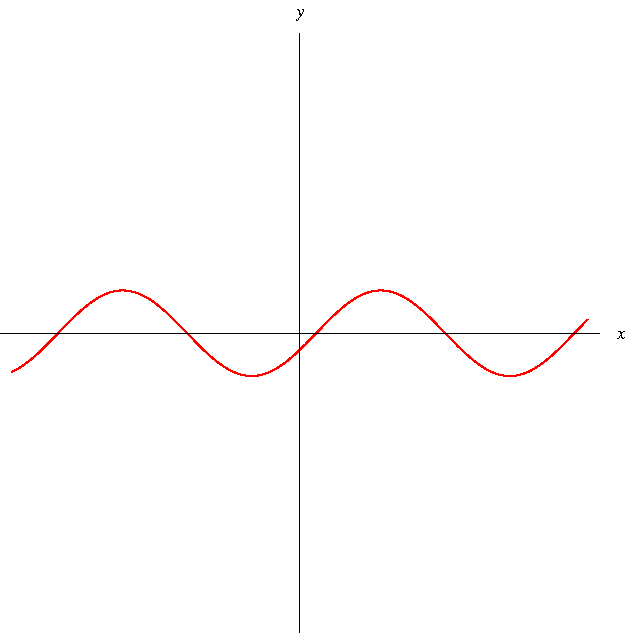
\includegraphics[height=3.8cm]{precalculus/pictures/01-02-vlt3.pdf} 
&%
\psset{xunit=0.33cm, yunit=0.33cm}
\begin{pspicture}(-5, -5)(5,5) 
\psframe*[linecolor=white](-5,-5)(5,5) 
\psaxes[ticks=none, labels=none]{<->}(0,0)(-4.5,-4.5)(4.5,4.5)\parametricplot[linecolor=red, plotpoints=1000]{0.05}{3}{t t 2.2 mul 57.29578 mul sin 1 add add t 57.29578 mul cos mul t t 2.2 mul 57.29578 mul sin 1 add add t 57.29578 mul sin mul}
\only<handout| 6->{%
\psline(1.7, -4.5)(1.7, 4.5)
}
\end{pspicture}
%\only<handout:0| -2>{%
%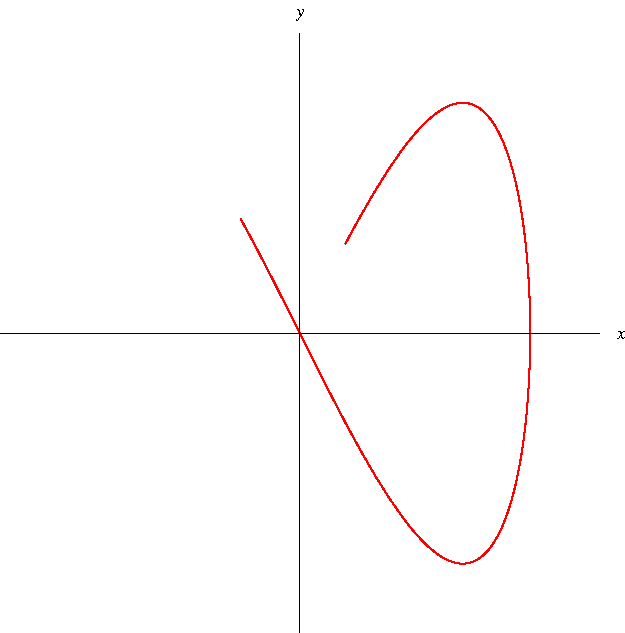
\includegraphics[height=3.8cm]{precalculus/pictures/01-02-vlt1a.pdf}%
%}%
%\only<handout| 3->{%
%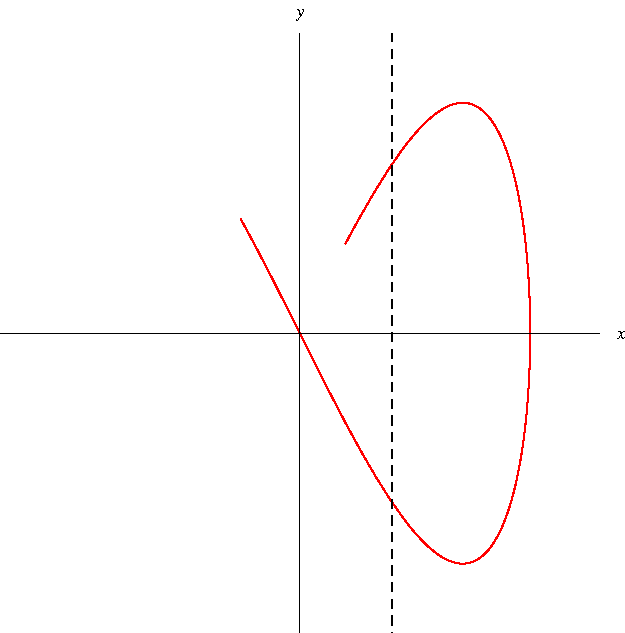
\includegraphics[height=3.8cm]{precalculus/pictures/01-02-vlt1b.pdf}%
%} 
&%
\psset{xunit=0.33cm, yunit=0.33cm}
\begin{pspicture}(-5, -5)(5,5) 
\psframe*[linecolor=white](-5,-5)(5,5) 
\psaxes[ticks=none, labels=none]{<->}(0,0)(-4.5,-4.5)(4.5,4.5)\tiny
%Function formula: 3/8+3/2 ((x)^{2})+1/4 (x)- ((x)^{3}) 
\psplot[linecolor=red, plotpoints=1000]{-0.5}{2}{x 3 exp -1 mul x 0.25 mul x 2 exp 1.5 mul 0.375 add add add } %Function formula: 1+1/2 (x) 
\psplot[linecolor=red, plotpoints=1000]{-4}{-0.5}{x 0.5 mul 1 add }
\end{pspicture} 
%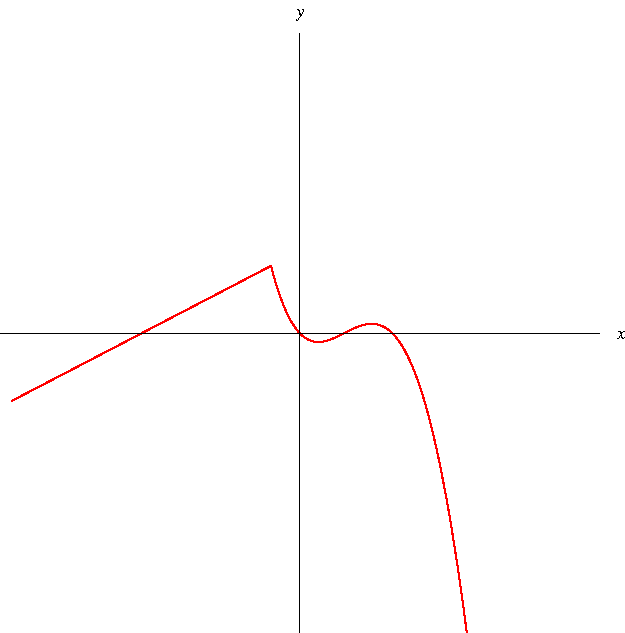
\includegraphics[height=3.8cm]{precalculus/pictures/01-02-vlt2.pdf} 
\\%
\fcAnswerUncoverNoH{1}{4}{Function} &
\fcAnswerUncoverNoH{1}{6}{Not a function}&
\fcAnswerUncoverNoH{1}{8}{Function}
\end{tabular}
\end{frame}
% end module vertical-line-test

\subsection{Piecewise Defined Functions}
% begin module function-piecewise
\begin{frame}
\frametitle{Piecewise Defined Functions}
\begin{definition}[Piecewise Defined Function]
A piecewise defined function is a function that is defined by different algebraic formulas on different subsets of its domain.
\end{definition}
\uncover<2->{
\begin{example}
\begin{columns}[t]
\column{.4\textwidth}
\psset{xunit=0.8cm, yunit=0.8cm}
\begin{pspicture}(-5, -5)(5,5) 
\psframe*[linecolor=white](-5,-5)(5,5) 
\psaxes[ticks=none, labels=none]{<->}(0,0)(-3,-1.5)(3,1.5)\tiny
\psLabelsWithOnes{3}{1.5}
\psline[linecolor=red](-3, -1)(0,-1)
\psline[linecolor=red](3, 1)(0,1)
\psHollowDot{0}{-1}
\psFullDot{0}{1}
\end{pspicture} 
%\ 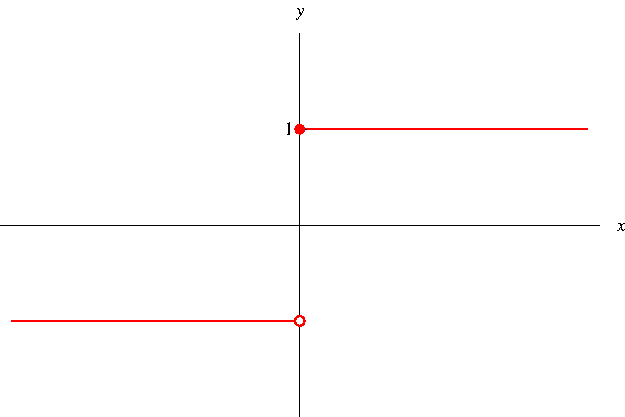
\includegraphics[height=3.5cm]{precalculus/pictures/01-01-piecewise.pdf}
\column{.5\textwidth}
\[
f(x) = \left\{ \begin{array}{rcc}
1 & \textrm{ if } & x \geq 0 \\
-1 & \textrm{ if } & x < 0 
\end{array}\right. 
\]

The filled red circle means $(0,1)$ is on the curve.  

The open circle means $(0, -1)$ is not on the curve.
\end{columns}
\end{example}
}
\end{frame}
% end module function-piecewise

% begin module absolute-value
\begin{frame}
\begin{example}
The absolute value $|x|$ of a number $a$ is defined to be
\[
|x| = \left\{ \begin{array}{ccccl}
\alertNoH{ 2-3}{x} & \alertNoH{ 3}{\text{if}} & \alertNoH{ 3}{x} & \alertNoH{ 3}{\geq} & \alertNoH{ 3}{0} \\
\alertNoH{ 4-5}{-x} & \alertNoH{ 5}{\text{if}} &  \alertNoH{ 5}{x} & \alertNoH{ 5}{<} & \alertNoH{ 5}{0}. \end{array}\right.
\]

Sketch a graph of the function $f(x) = |x|$.

%no begin{center} due to bug!
\hfil\hfil
\psset{xunit=1.2cm, yunit=1.2cm}
\begin{pspicture}(-3.2, -0.5)(3.2,3.2)
\tiny
\psframe*[linecolor=white](-3.2,-0.5)(3.2,3.2)
\psaxes[ticks=none, labels=none]{<->}(0,0)(-3,-0.5)(3,3)
\fcLabelsWithOnes{3}{3}
\uncover<handout:0|2>{
\psline[linecolor=blue](-0.5, -0.5)(3,3)
}
\uncover<3->{
\psline[linecolor=red](0,0)(3,3)
}
\uncover<handout:0|4>{
\psline[linecolor=blue](-3, 3)(0.5,-0.5)
}
\uncover<5->{
\psline[linecolor=red](-3, 3)(0,0)
}
\end{pspicture}
\end{example}
\end{frame}
% end module absolute-value

% begin module piecewise-formula
\begin{frame}
\begin{example} %[Example 9, p. 18]
Find a formula for the function $f$ in the graph.

\psset{xunit=1.2cm, yunit=1.2cm}
\begin{pspicture}(-0.5, -0.5)(5.3,2.4)
\tiny
\psframe*[linecolor=white](-0.5,-0.5)(5.2,2.4)
\psaxes{<->}(0,0)(-0.5,-0.5)(5.2,2.2)
\fcLabels{5.1}{2.2}
\psline[linecolor=red](0,0)(1,1)(2,0)(5,0)
\fcHollowDot{5}{0}
\fcFullDot{0}{0}
\only<handout:0|4-5>{
\psline[linecolor=blue](-0.5, -0.5)(2,2)
}
\only<handout:0|6-7>{
\psline[linecolor=blue](-0.2, 2.2)(2.5,-0.5)
}
\only<handout:0|8-9>{
\psline[linecolor=blue](2, 0)(5,0)
}
\end{pspicture}
%\ \only<1-3,10>{%
%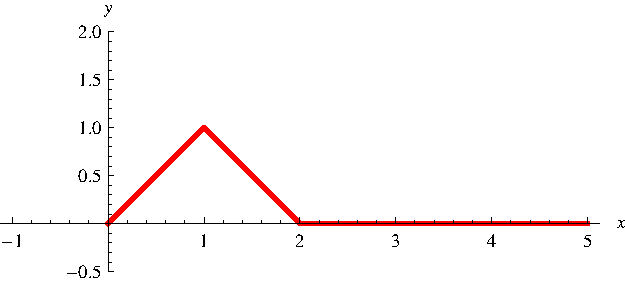
\includegraphics[height=4cm]{precalculus/pictures/01-01-ex-09a.pdf}%
%}%
%\only<handout:0| 4-5>{%
%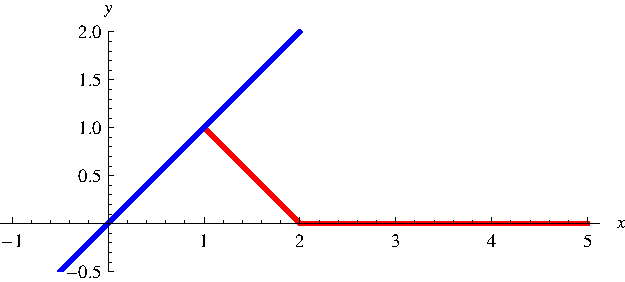
\includegraphics[height=4cm]{precalculus/pictures/01-01-ex-09b.pdf}%
%}%
%\only<handout:0| 6-7>{%
%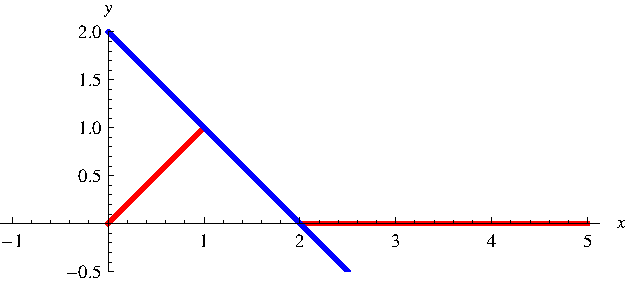
\includegraphics[height=4cm]{precalculus/pictures/01-01-ex-09c.pdf}%
%}%
%\only<handout:0| 8-9>{%
%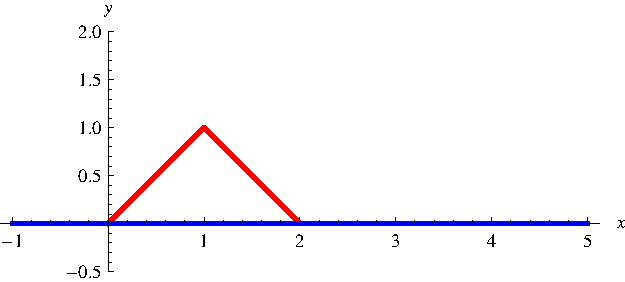
\includegraphics[height=4cm]{precalculus/pictures/01-01-ex-09d.pdf}%
%}%

\uncover<2->{
Different formulas on $[0, 1)$, $[1, 2)$, and $[2, 5)$.
}

\uncover<3->{
\[
f(x) = \left\{ \begin{array}{ccccccl}
\uncover<5->{\alert<handout:0| 5>{x}} & \alert<handout:0| 4-5>{\textrm{if}} & \alert<handout:0| 4-5>{0} & \alert<handout:0| 4-5>{\leq} & \alert<handout:0| 4-5>{x} & \alert<handout:0| 4-5>{<} & \alert<handout:0| 4-5>{1} \\
\uncover<7->{\alert<handout:0| 7>{2 - x}} & \alert<handout:0| 6-7>{\textrm{if}} & \alert<handout:0| 6-7>{1} & \alert<handout:0| 6-7>{\leq} & \alert<handout:0| 6-7>{x} & \alert<handout:0| 6-7>{<} & \alert<handout:0| 6-7>{2} \\
\uncover<9->{\alert<handout:0| 9>{0}} & \alert<handout:0| 8-9>{\textrm{if}} & \alert<handout:0| 8-9>{2} & \alert<handout:0| 8-9>{\leq} & \alert<handout:0| 8-9>{x} & \alert<handout:0| 8-9>{<} & \alert<handout:0| 8-9>{5} \end{array}\right.
\]
}
\end{example}
\end{frame}
% end module piecewise-formula

% begin module piecewise-ex1
\begin{frame}
\begin{example}
Sketch the function $f(x)  = |2x-3|$.
\begin{columns}
\column{.4\textwidth}
\only<-5| handout:0>{%
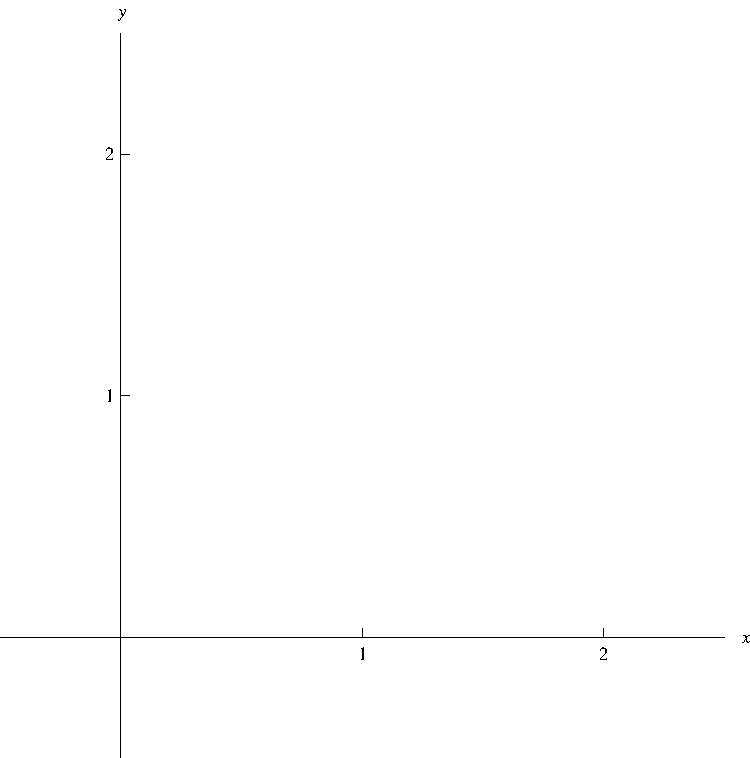
\includegraphics[width=4.5cm]{precalculus/pictures/piecewise-ex1-1.pdf}%
}%
\only<6| handout:0>{%
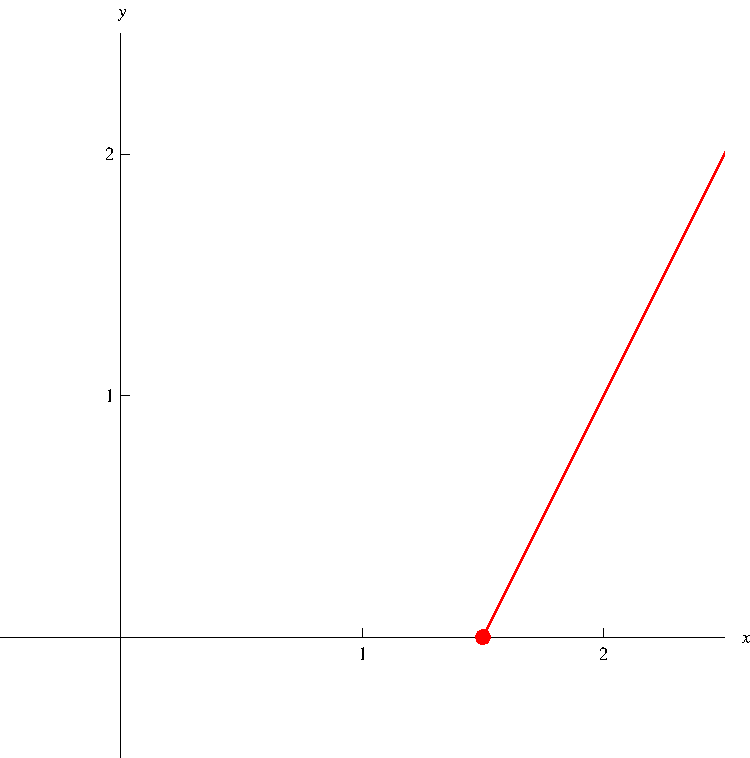
\includegraphics[width=4.5cm]{precalculus/pictures/piecewise-ex1-2.pdf}%
}%
\only<7-| handout:1>{%
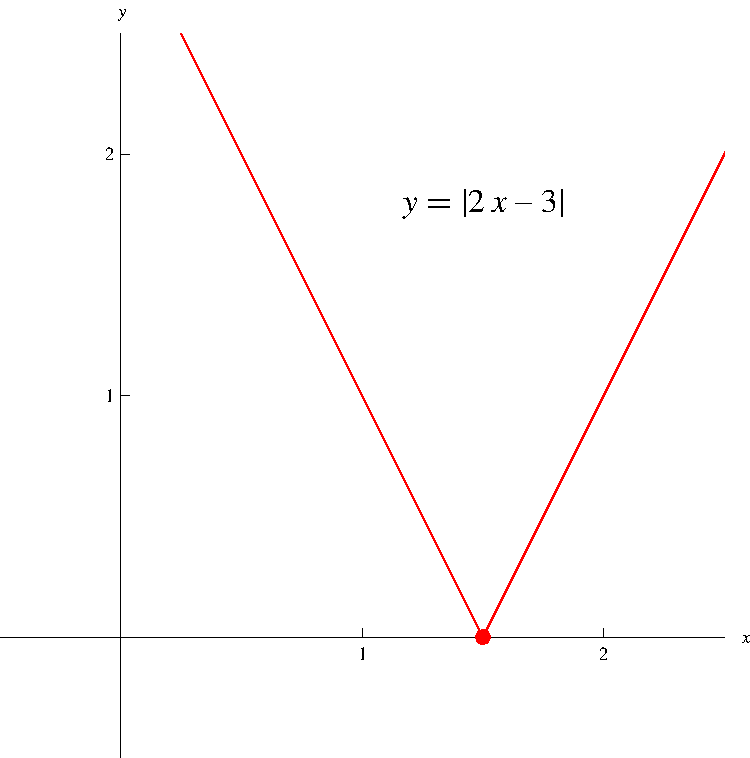
\includegraphics[width=4.5cm]{precalculus/pictures/piecewise-ex1-3.pdf}%
}%
\column{.55\textwidth}
\abovedisplayskip=0pt
\belowdisplayskip=-15pt
\abovedisplayshortskip=0pt
\belowdisplayshortskip=0pt
\begin{align*}
\uncover<2->{%
|\alert<handout:0| 3>{x}| %
}%
& \uncover<2->{%
 = \begin{cases}
\alert<handout:0| 3>{x} & \text{if $\alert<handout:0| 3>{x} \geq 0$}\\
-\alert<handout:0| 3>{x} & \text{if $\alert<handout:0| 3>{x} < 0$}.\\
\end{cases}
}\\%
\uncover<3->{%
|\alert<handout:0| 3>{2x-3}| %
}%
& \uncover<3->{%
 = \begin{cases}
\alert<handout:0| 3>{2x-3} & \text{if $\alert<handout:0| 3>{2x-3} \geq 0$}\\
-(\alert<handout:0| 3>{2x-3}) & \text{if $\alert<handout:0| 3>{2x-3} < 0$}\\
\end{cases}
}\\%
& \uncover<4->{%
 = \begin{cases}
2x-3 & \text{if $2x \geq 3$}\\
-2x+3 & \text{if $2x < 3$}\\
\end{cases}
}\\%
& \uncover<5->{%
 = \begin{cases}
\alert<handout:0| 6>{2x-3} & \alert<handout:0| 6>{\text{if $x \geq 3/2$}}\\
\alert<handout:0| 7>{-2x+3} & \alert<handout:0| 7>{\text{if $x < 3/2$}}.\\
\end{cases}
}%
\end{align*}
\end{columns}
\end{example}
\end{frame}
% end module piecewise-ex1

% begin module piecewise-ex2
\begin{frame}
\begin{example}
Sketch the function $\displaystyle f(x)  = \frac{|4x+2|}{2x+1}$.
\begin{columns}
\column{.4\textwidth}
\only<-8| handout:0>{%
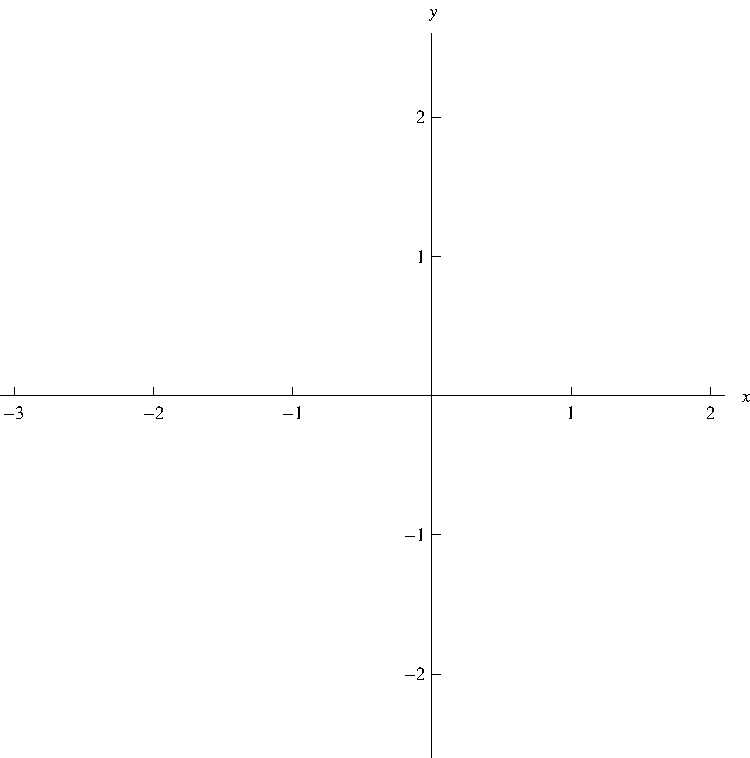
\includegraphics[width=4.5cm]{precalculus/pictures/piecewise-ex2-1.pdf}%
}%
\only<9| handout:0>{%
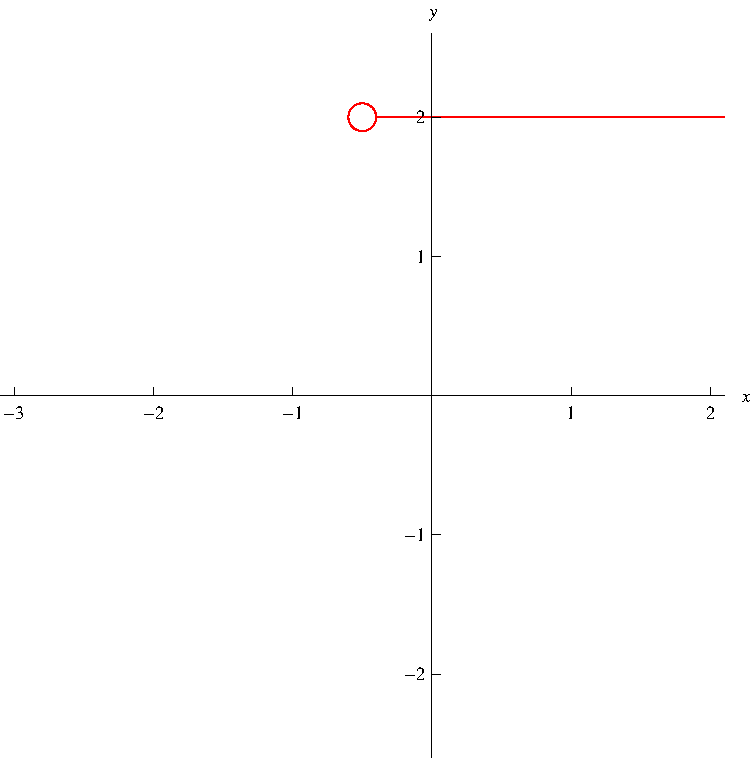
\includegraphics[width=4.5cm]{precalculus/pictures/piecewise-ex2-2.pdf}%
}%
\only<10-| handout:1>{%
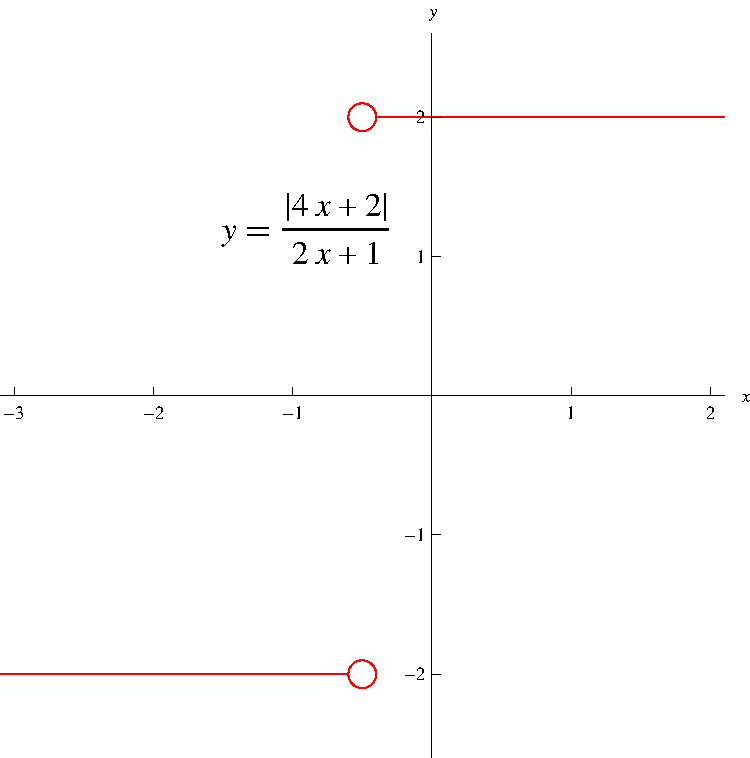
\includegraphics[width=4.5cm]{precalculus/pictures/piecewise-ex2-3.pdf}%
}%
\column{.55\textwidth}
\abovedisplayskip=0pt
\belowdisplayskip=-15pt
\abovedisplayshortskip=0pt
\belowdisplayshortskip=0pt
\begin{align*}
\uncover<2->{%
|\alert<handout:0| 3>{x}| %
}%
& \uncover<2->{%
 = \begin{cases}
\alert<handout:0| 3>{x} & \text{if $\alert<handout:0| 3>{x} \geq 0$}\\
-\alert<handout:0| 3>{x} & \text{if $\alert<handout:0| 3>{x} < 0$}.\\
\end{cases}
}\\%
\uncover<3->{%
\frac{|\alert<handout:0| 3>{4x+2}|}{2x+1} %
}%
& \uncover<3->{%
 = \begin{cases}
\frac{\alert<handout:0| 3-5>{4x+2}}{2x+1} & \text{if $\alert<handout:0| 3>{4x+2} > 0$}\\
\frac{\alert<handout:0| 6-7>{-(\alert<handout:0| 3>{4x+2})}}{2x+1} & \text{if $\alert<handout:0| 3>{4x+2} < 0$}\\
\end{cases}
}\\%
& \uncover<4->{%
 = \begin{cases}
\frac{\uncover<5->{\alert<handout:0| 5>{2(2x+1)}}}{2x+1} & \text{if $4x > -2$}\\
\frac{\uncover<7->{\alert<handout:0| 7>{-2(2x+1)}}}{2x+1} & \text{if $4x < -2$}\\
\end{cases}
}\\%
& \uncover<8->{%
 = \begin{cases}
\alert<handout:0| 9>{2} & \alert<handout:0| 9>{\text{if $x > -1/2$}}\\
\alert<handout:0| 10>{-2} & \alert<handout:0| 10>{\text{if $x < -1/2$}}.\\
\end{cases}
}%
\end{align*}
\end{columns}
\end{example}
\end{frame}
% end module piecewise-ex2

\subsection{Symmetry}
% begin module even-and-odd
\begin{frame}
\frametitle{Symmetry}
\begin{definition}[Even and Odd Functions]
A function $f$ is called even if $f(-x) = f(x)$ for all $x$ in its domain.  A function $f$ is called odd if $f(-x) = -f(x)$ for all $x$ in its domain.
\end{definition}
\uncover<2->{
\begin{example}[$x^2$ is Even, $x^3$ is Odd]
The function $f(x) = x^2$ is even:
\uncover<3->{
\[
f(-x) = (-x)^2 = x^2 = f(x) .
\]
}
The function $g(x) = x^3$ is odd:
\uncover<4->{
\[
g(-x) = (-x)^3 = -x^3 = -g(x) .
\]
}
\end{example}
}
\end{frame}

\begin{frame}
\begin{definition}[Even and Odd Functions]
A function $f$ is called even if $f(-x) = f(x)$ for all $x$ in its domain.  A function $f$ is called odd if $f(-x) = -f(x)$ for all $x$ in its domain.
\end{definition}
\begin{example} %[Example 11, p. 19]
Determine whether each of the following functions is even, odd, or neither even nor odd.

\begin{columns}[t]
\column{.33\textwidth}
\[
f(x) = x^5 + x
\]
\[
\begin{array}{r@{ \ }c@{ \ }l}
\uncover<2->{f(-x)} & \uncover<2->{=} & \uncover<3->{(-x)^5 + (-x)} \\
& \uncover<4->{=} & \uncover<4->{-x^5 - x} \\
& \uncover<5->{=} & \uncover<5->{-(x^5 + x)} \\
& \uncover<6->{=} & \uncover<6->{-f(x)} 
\end{array}
\]
\uncover<7->{
Therefore $f$ is odd.
}
\column{.33\textwidth}
\[
g(x) = 1 - x^4
\]
\[
\begin{array}{r@{ \ }c@{ \ }l}
\uncover<2->{g(-x)} & \uncover<2->{=} & \uncover<8->{1 - (-x)^4} \\
& \uncover<9->{=} & \uncover<9->{1 - x^4} \\
& \uncover<10->{=} & \uncover<10->{g(x)} 
\end{array}
\]
\uncover<11->{
Therefore $g$ is even.
}
\column{.33\textwidth}
\[
h(x) = 2x - 1
\]
\[
\begin{array}{r@{ \ }c@{ \ }l}
\uncover<2->{h(-x)} & \uncover<2->{=} & \uncover<12->{2(-x) - 1} \\
& \uncover<13->{=} & \uncover<13->{-2x - 1} \\
& \uncover<14->{\neq} & \uncover<14->{h(x), -h(x)}
\end{array}
\]
\uncover<15->{
Therefore $h$ is neither even nor odd.
}
\end{columns}
\end{example}
\end{frame}
% end module even-and-odd

\subsection{Increasing and Decreasing Functions}
% begin module increasing-decreasing
\begin{frame}
\frametitle{Increasing and Decreasing Functions}
\begin{definition}[Increasing and Decreasing Functions]
A function $f$ is called increasing on an interval $I$ if $f(x_1) < f(x_2)$ whenever $x_1 < x_2$  in $I$.

It is called decreasing on the interval $I$ if $f(x_1) > f(x_2)$ whenever $x_1 < x_2$ in $I$.
\end{definition}
\uncover<2->{
\begin{example}[Increasing and Decreasing]
\begin{columns}[t]
\column{.6\textwidth}

\psset{xunit=3.4cm, yunit=3.4cm}
\begin{pspicture}(-1.1, -0.4)(1.15,0.7)
\psframe*[linecolor=white](-1.1,-0.4)(1.15,0.7)
\tiny
\psaxes[Dx=0.25, Dy=0.25]{<->}(0,0)(-1.1,-0.3)(1.1,0.6)
\fcLabels{1.1}{0.6}
%Function formula: 7/40+13/10 ((x)^{3})-39/40 (x)
\psplot[linecolor=red, plotpoints=1000]{-1}{1}{x -0.975 mul x 3 exp 1.3 mul 0.175 add add }
\uncover<handout:0|3>{
\psplot[linecolor=blue, plotpoints=1000]{-1}{-0.5}{x -0.975 mul x 3 exp 1.3 mul 0.175 add add }
}
\uncover<handout:0|4>{
\psplot[linecolor=blue, plotpoints=1000]{-0.5}{0.5}{x -0.975 mul x 3 exp 1.3 mul 0.175 add add }
}
\uncover<handout:0|5>{
\psplot[linecolor=blue, plotpoints=1000]{0.5}{1}{x -0.975 mul x 3 exp 1.3 mul 0.175 add add }
}
\end{pspicture}
%\ \only<-2>{%
%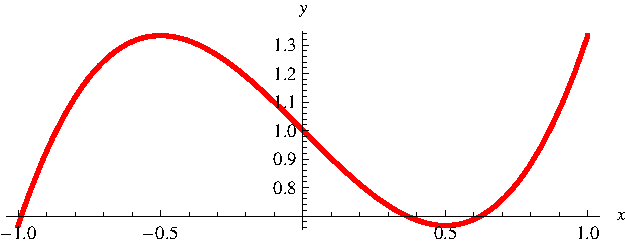
\includegraphics[height=2.8cm]{precalculus/pictures/01-01-inc-dec-a.pdf}%
%}%
%\only<handout:0| 3>{%
%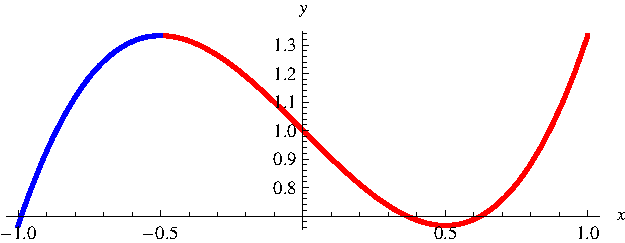
\includegraphics[height=2.8cm]{precalculus/pictures/01-01-inc-dec-b.pdf}%
%}%
%\only<handout:0| 4>{%
%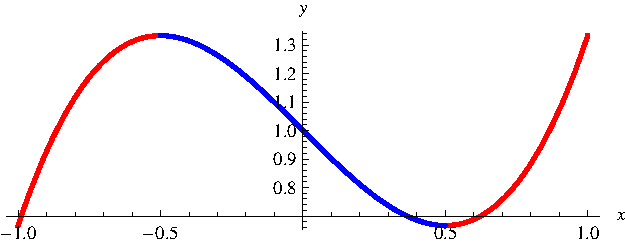
\includegraphics[height=2.8cm]{precalculus/pictures/01-01-inc-dec-c.pdf}%
%}%
%\only<handout:0| 5->{%
%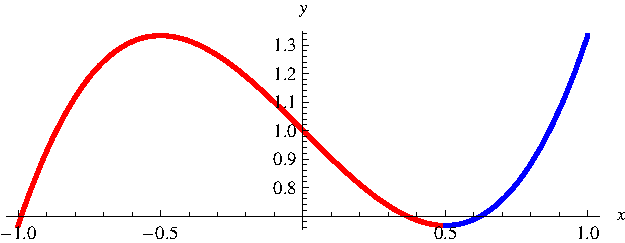
\includegraphics[height=2.8cm]{precalculus/pictures/01-01-inc-dec-d.pdf}%
%}%
\column{.4\textwidth}
\begin{itemize}
\item<3-| alert@3> \only<handout:0|3>{\color{blue}} $f$ is increasing on $[-1, -\frac{1}{2}]$.
\item<4-| alert@4> \only<handout:0|4>{\color{blue}} $f$ is decreasing on $[-\frac{1}{2}, \frac{1}{2}]$.
\item<5-| alert@5> \only<handout:0|5>{\color{blue}} $f$ is increasing on $[\frac{1}{2}, 1]$.
\end{itemize}
\end{columns}
\end{example}
}
\end{frame}
% end module increasing-decreasing

\subsection{A Note on Domains of Functions}
% begin module domains
\begin{frame}
\frametitle{A Note on Domains of Functions}
If the domain of a function isn't specified, it is implied to be all numbers $x$ for which the formula $f(x)$ is defined. There are some restrictions to consider:
\begin{itemize}
\item<2->  Can't divide by $0$.
\item<3->  Even roots of a negative number are not defined in this course ($\sqrt{-1} , \sqrt[4]{-2053}, \sqrt[6]{-15} \ldots$ not allowed).
\item<4->  Taking $\log x$ if $x \leq 0$ is not allowed in this course; taking  $\log 0$ is not allowed in any course.
\end{itemize}
\end{frame}


% end module domains

}% end lecture

\lect{Fall 2015}{Sections 1.2 and 1.3}{2}{% begin lecture
%DesiredLectureName: Catalog_Essential_Functions_Constructing_Functions
\section{1.2 A Catalog of Essential Functions}
\subsection{Linear Functions}
% begin module linear-functions
\begin{frame}
\frametitle{Linear Functions}
\begin{definition}[Linear Function]
A linear function is a function the graph of which is a line.  We can write any linear function in slope-intercept form:
\[
f(x) = mx + b.
\]
$m$ is called the slope, and $b$ is called the $y$-intercept.
\end{definition}
\end{frame}

\begin{frame}
\begin{columns}[c]
\column{.5\textwidth}

\psset{xunit=0.7cm, yunit=0.7cm}
\begin{pspicture}(-2.6, -2.5)(5,2.6)
\psframe*[linecolor=white](-2.6,-2.5)(4.1,2.6)
\tiny
\fcAxesStandard{-2.6}{-2.5}{5}{2.6}
\fcLabelXOne
\uncover<2>{
\psline[linecolor=red](-2.5, -1.5)(1.5, 2.5)
}
\uncover<3->{
\psline[linecolor=blue](-2.5, -1.5)(1.5, 2.5)
}
\uncover<2->{
\rput[l](1.5, 2){$y=x+1$}
}
\uncover<5->{
\fcFullDot{0}{1}
\rput[r](-0.1, 1){\alert<5>{$(0,1)$}}
}

\uncover<3>{
\psline[linecolor=red](-2.5, 1.25)(5, -2.5)
}
\uncover<4->{
\psline[linecolor=blue](-2.5, 1.25)(5, -2.5)
}
\uncover<3->{
\rput[r](3.3, -2){$y=-0.5x$}
}
\uncover<6->{
\fcFullDot{0}{0}
\rput[lb](0.1, 0.1){\alert<6>{$(0,0)$}}
}

\uncover<4>{
\psline[linecolor=red](-2.5,-1)(5, -1)
}
\uncover<5->{
\psline[linecolor=blue](-2.5, -1)(5, -1)
}
\uncover<4->{
\rput[t](4, -1.1){$y=-1$}
}
\uncover<7->{
\fcFullDot{0}{-1}
\rput[lt](0.1, -1.1){\alert<7>{$(0,-1)$}}
}
\end{pspicture}
\column[t]{.55\textwidth}
\begin{tabular}{|c|c|c|}
\hline
$f(x)$ & Direction & $y$-intercept \\
\hline
\uncover<1->{\alert<handout:0| 2>{$x + \alert<handout:0| 5>{1}$}} &
\uncover<2->{\alert<handout:0| 2>{$\nearrow$}} &
\uncover<5->{\alert<handout:0| 5>{1}} \\
\uncover<1->{\alert<handout:0| 3>{$-0.5x \uncover<6>{\alert<handout:0| 6>{+ 0}}$}} &
\uncover<3->{\alert<handout:0| 3>{$\searrow$}} &
\uncover<6->{\alert<handout:0| 6>{0}} \\
\uncover<1->{\alert<handout:0| 4,7>{$-1$}} &
\uncover<4->{\alert<handout:0| 4>{$\rightarrow$}} &
\uncover<7->{\alert<handout:0| 7>{-1}} \\
\hline
\end{tabular}
\end{columns}

\begin{itemize}
\item<2->  $m > 0$ means the graph of $f$ points up ($\nearrow$).
\item<3->  $m < 0$ means the graph of $f$ points down ($\searrow$).
\item<4->  $m = 0$ means the graph of $f$ is horizontal ($\rightarrow$).
\item<5->  $b$ tells us the height of the point where the graph hits the $y$-axis.
\end{itemize}
\end{frame}
% end module linear-functions

\subsection{Polynomials}
% begin module polynomials
\begin{frame}
\frametitle{Polynomials}
\begin{definition}[Polynomial Function]
A polynomial function is a function $f$ of the form
\[
f(x) = a_0 + a_1x + a_2x^2 + \cdots + a_{n - 1}x^{n-1} + a_nx^n ,
\]
where $n$ is a non-negative integer and $a_0, \ldots , a_n$ are real numbers, called the coefficients.

If the leading coefficient $a_n \neq 0$, then we say the degree of $f$ is $n$.
\end{definition}
\uncover<2->{
\[
\begin{array}{|c|c|c|c|c|c|}
\hline
f(x) &%
\alert<handout:0| 3-4,13-14,23-26,35-36>{\text{Polynomial?}} &%
\alert<handout:0| 5-6,15-16,27-28>{\text{Degree}} &%
\alert<handout:0| 7-8,17-18,29-30>{a_0} &%
\alert<handout:0| 9-10,19-20,31,32>{a_1} &%
\alert<handout:0| 11-12,21-22,33-34>{a_2} \\
\hline
\alert<handout:0| 3-12>{x^4-x+1} &%
\uncover<4->{\alert<handout:0| 4>{\text{Yes}}}&%
\uncover<6->{\alert<handout:0| 6>{4}}&%
\uncover<8->{\alert<handout:0| 8>{1}}&%
\uncover<10->{\alert<handout:0| 10>{-1}}&%
\uncover<12->{\alert<handout:0| 12>{0}}\\%
\alert<handout:0| 13-22>{6} &%
\uncover<14->{\alert<handout:0| 14>{\text{Yes}}}&%
\uncover<16->{\alert<handout:0| 16>{0}}&%
\uncover<18->{\alert<handout:0| 18>{6}}&%
\uncover<20->{\alert<handout:0| 20>{0}}&%
\uncover<22->{\alert<handout:0| 22>{0}}\\%
\alert<handout:0| 23>{3x^2 - \frac{1}{2}x + \alert<handout:0| 24>{\sqrt{x}}} &%
\uncover<24->{\alert<handout:0| 24>{\text{No}}}&%
&%
&%
&\\
\alert<handout:0| 25-34>{3x^2 - \frac{1}{2}x + \sqrt{2}} &%
\uncover<26->{\alert<handout:0| 26>{\text{Yes}}}&%
\uncover<28->{\alert<handout:0| 28>{2}}&%
\uncover<30->{\alert<handout:0| 30>{\sqrt{2}}}&%
\uncover<32->{\alert<handout:0| 32>{-\frac{1}{2}}}&%
\uncover<34->{\alert<handout:0| 34>{3}}\\%
\alert<handout:0| 35>{3x^2 - \frac{1}{2\alert<handout:0| 36>{x}} + \sqrt{2}} &%
\uncover<36->{\alert<handout:0| 36>{\text{No}}}&%
&%
&%
&\\
\hline
\end{array}
\]
}
\end{frame}


\begin{frame}
\begin{itemize}
\item<1->  Linear functions are polynomials.
\item<2->  So are quadratic functions.  Their graphs are parabolas.
\item<3->  And there are many more.
\end{itemize}
\only<handout:1| 1>{%
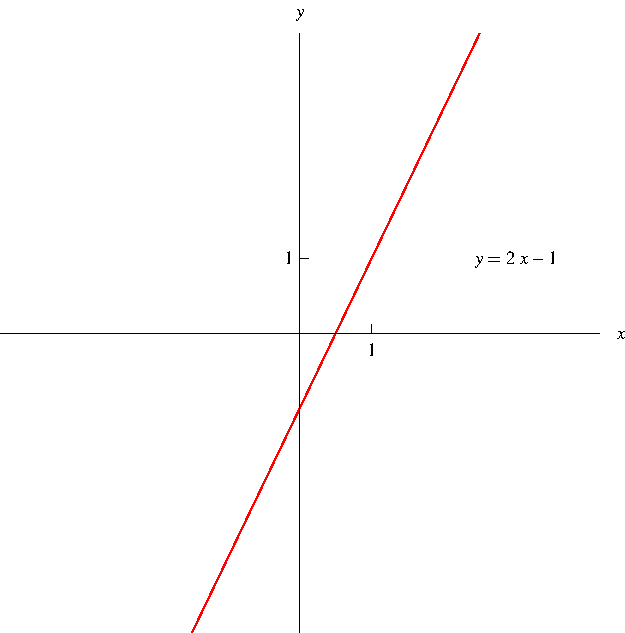
\includegraphics[height=6cm]{precalculus/pictures/01-02-line.pdf}%

Linear
}%
\only<handout:2| 2>{%
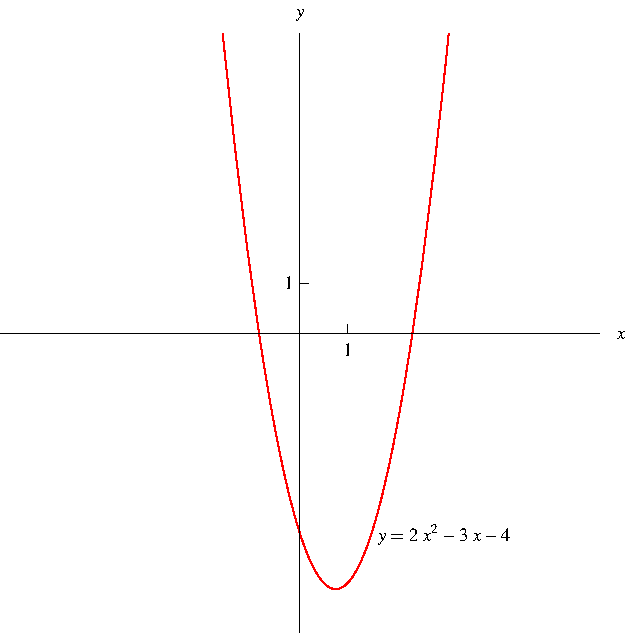
\includegraphics[height=6cm]{precalculus/pictures/01-02-parabola.pdf}%

Quadratic
}%
\only<handout:3| 3>{%
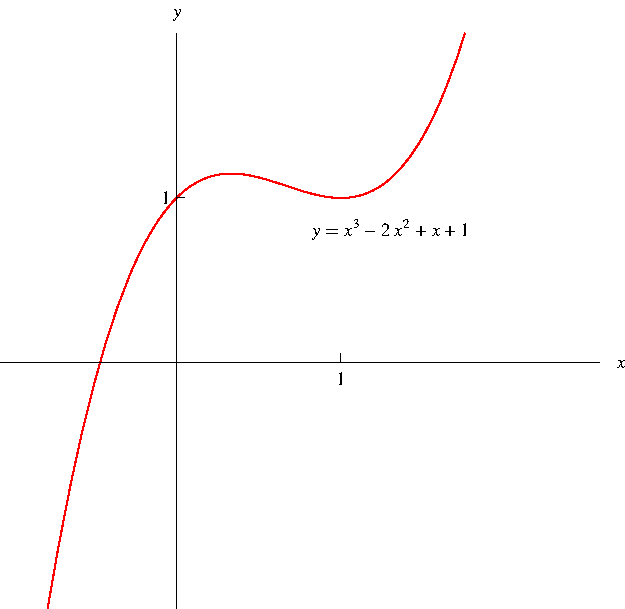
\includegraphics[height=6cm]{precalculus/pictures/01-02-polya.pdf}%

Cubic
}%
\only<handout:4| 4>{%
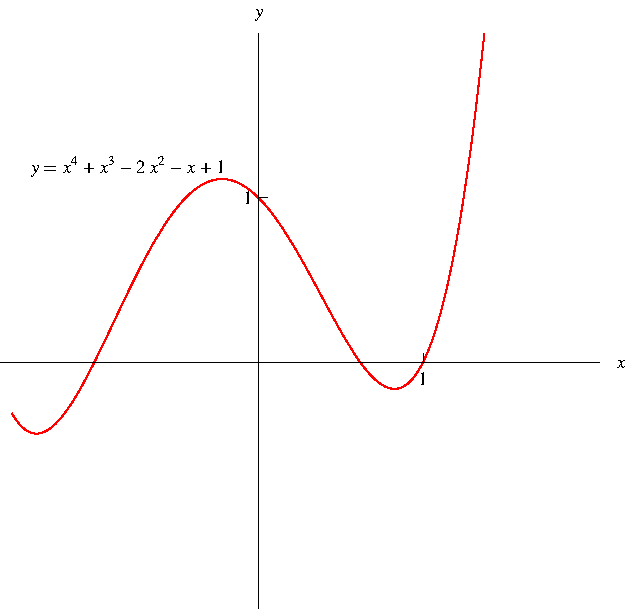
\includegraphics[height=6cm]{precalculus/pictures/01-02-polyb.pdf}%

Quartic
}%
\only<handout:5| 5>{%
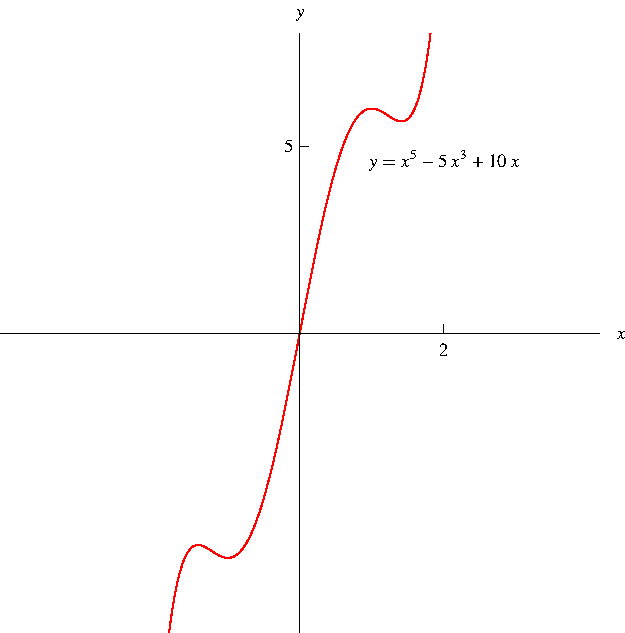
\includegraphics[height=6cm]{precalculus/pictures/01-02-polyc.pdf}%

Quintic
}
\end{frame}
% end module polynomials

\subsection{Power Functions}
%Old Version from Greg. Greg, this slide is changed substantially, please take a look.
%% begin module power-functions-def
%\begin{frame}
%\frametitle{Power Functions}
%\begin{definition}[Power Function]
%A power function is a function of the form
%\[
%f(x) = x^a,
%\]
%where $a$ is a fixed real number.
%\end{definition}
%\uncover<2->{
%If $a$ is a positive integer like $1, 2, 3, \ldots$ then $x^a$ is a polynomial.

%\only<handout:-2| -2>{%
%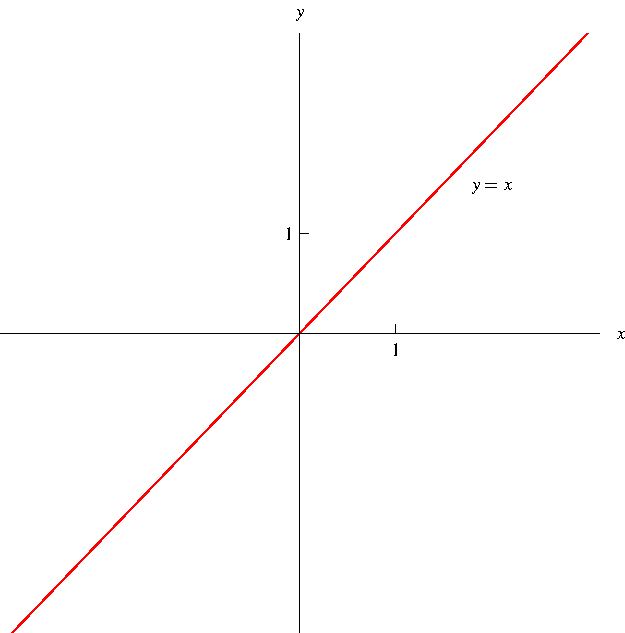
\includegraphics[height=4cm]{precalculus/pictures/01-02-x.pdf}%
%}%
%\only<handout:3| 3>{%
%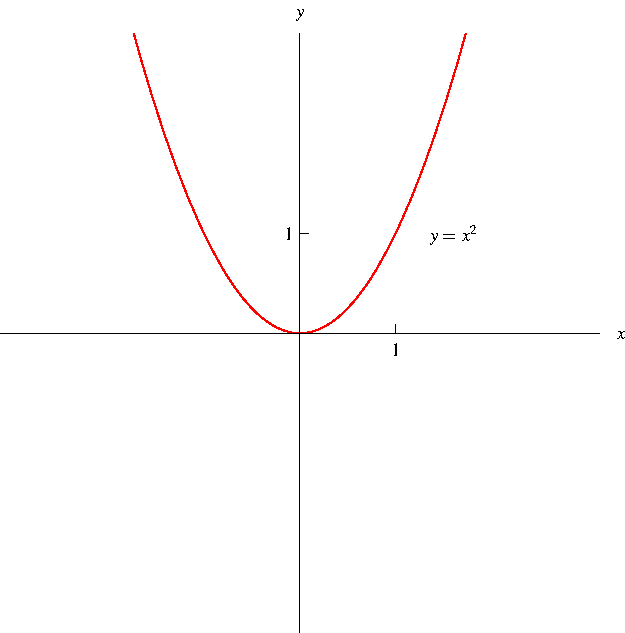
\includegraphics[height=4cm]{precalculus/pictures/01-02-xsquared.pdf}%
%}%
%\only<handout:4| 4>{%
%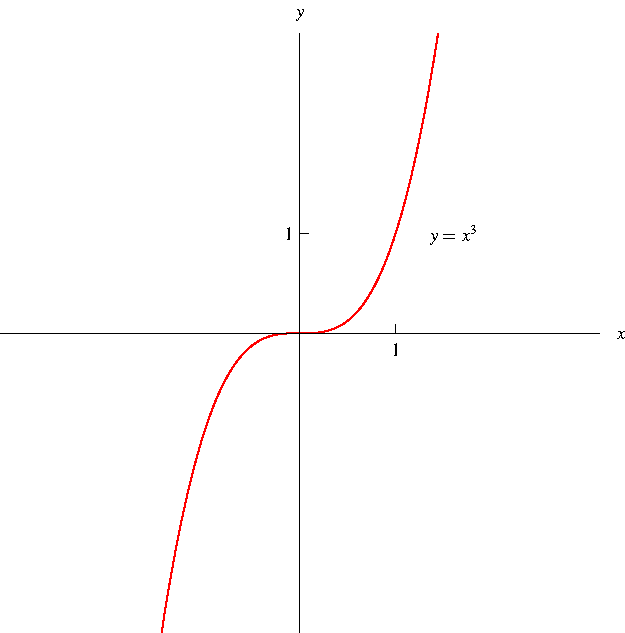
\includegraphics[height=4cm]{precalculus/pictures/01-02-xcubed.pdf}%
%}%
%\only<handout:5| 5>{%
%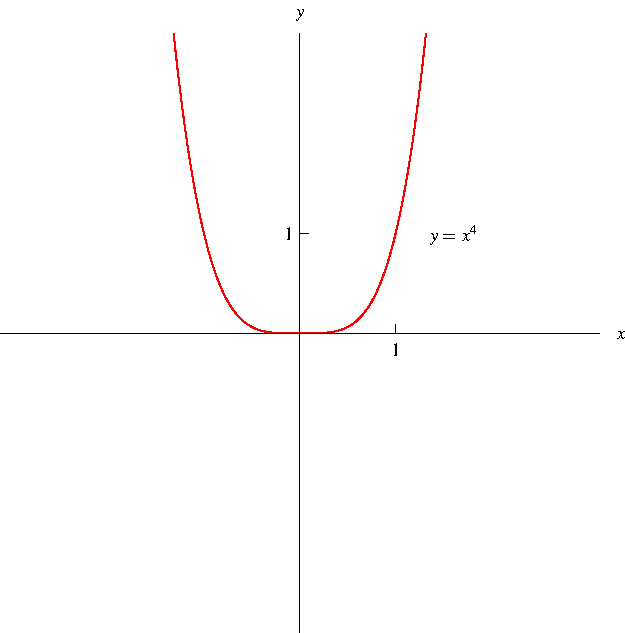
\includegraphics[height=4cm]{precalculus/pictures/01-02-xfourth.pdf}%
%}%
%\only<handout:6| 6>{%
%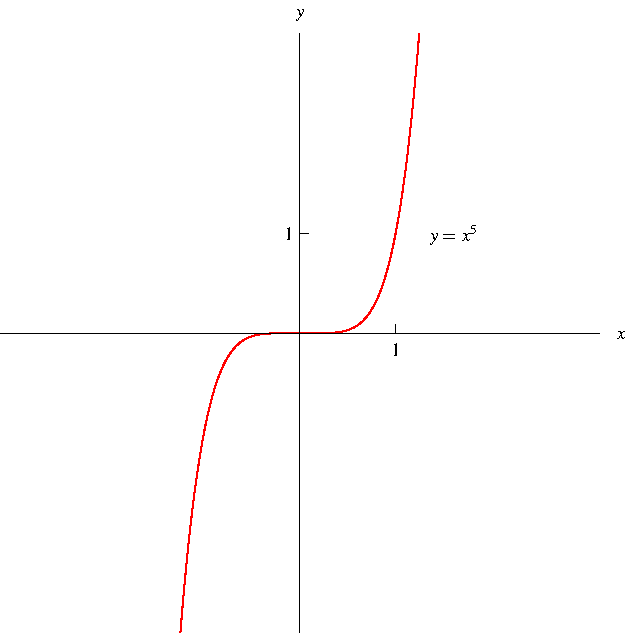
\includegraphics[height=4cm]{precalculus/pictures/01-02-xfifth.pdf}
%}%
%}%
%\end{frame}
%% end module power-functions-def

% begin module power-functions-def
\begin{frame}[t]
\frametitle{Power Functions}
\begin{definition}[Power Function]
Let $x>0$, $a$ - arbitrary real number. The power function is defined as
\[
f(x) \uncover<4->{\alert<handout: 0| 4>{=e^{a\ln x} } }= \alert<2>{x}^{\alert<3>{a}} \quad .
\]
\uncover<2->{$x$ = \alert<2>{base}. } \uncover<3->{$a$ = \alert<3>{exponent} or \alert<3>{power}. }
\uncover<4->{\alert<handout:0| 4>{First equality = one of ways to define for non-integer $a$ (we study $\ln x$, $e^x$ later). } }
\end{definition}
\begin{tabular}{l}
\uncover<5->{
If $a$ - positive integer ($1, 2, 3, \ldots$) \\
then $x^a$ = polynomial function.
}\\
\uncover<5->{
$x^{n}    =\underbrace{x\dots x }_{n~\mathrm{times}}$ when $n$-integer. \\
$\alert<12>{(x^{a})^b}=\uncover<13->{\alert<13>{x^{ab}}}$  \\
$\alert<14>{(xy)^b}   =\uncover<15->{\alert<15>{x^by^b}}$\\
$\alert<16>{x^{a+b}}  =\uncover<17->{\alert<17>{x^ax^b }}$ \\
$\alert<18>{x^{-a}}   =\uncover<19->{\alert<19>{\frac{1}{x^a}}}$\\
~\\~\\~\\~\\~\\~\\~\\
}
\end{tabular}
\uncover<6->{
\psset{xunit=0.38cm,yunit=0.38cm}
\begin{pspicture}(-5,-5)(5,5)
\psaxes[labels=none]{<->}(0,0)(-5,-5)(5,5)
\tiny
\rput[r](0,5){\tiny{$y$}}
\rput[l](5,0){\tiny{$x$}}
\only<7>{
\psplot[linecolor=red]{-5}{5}{ x 1 exp }
\rput( 3, 1){$y=x^{\phantom{1}}$}
} %only
\only<8>{
\psplot[linecolor=red]{-2.23}{2.23}{ x 2 exp }
\rput( 3, 1){$y=x^2$}
}
\only<9>{
\psplot[linecolor=red]{-1.7}{1.7}{ x 3 exp }
\rput( 3, 1){$y=x^3$}
}
\only<10>{
\psplot[linecolor=red]{-1.49}{1.49}{ x 4 exp }
\rput( 3, 1){$y=x^4$}
}
\only<11->{
\psplot[linecolor=red]{-1.37}{1.37}{ x 5 exp }
\rput( 3, 1){$y=x^5$}
}
\end{pspicture}
%\only<handout:-2| -2>{%
%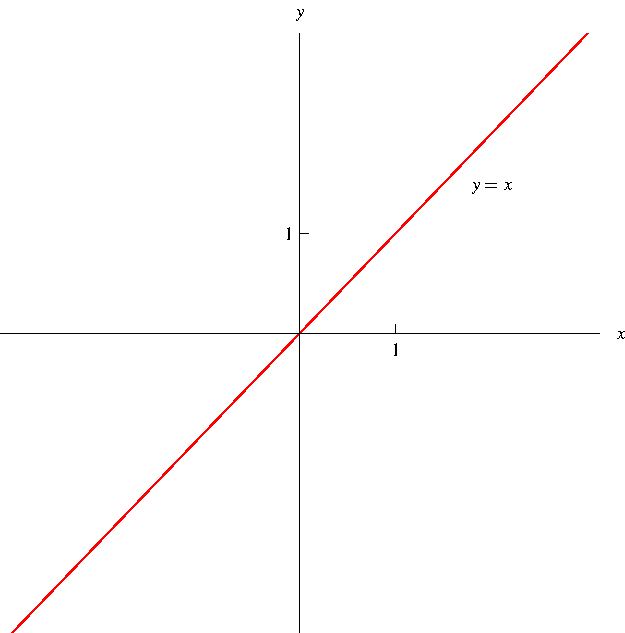
\includegraphics[height=4cm]{precalculus/pictures/01-02-x.pdf}%
%}%
%\only<handout:3| 3>{%
%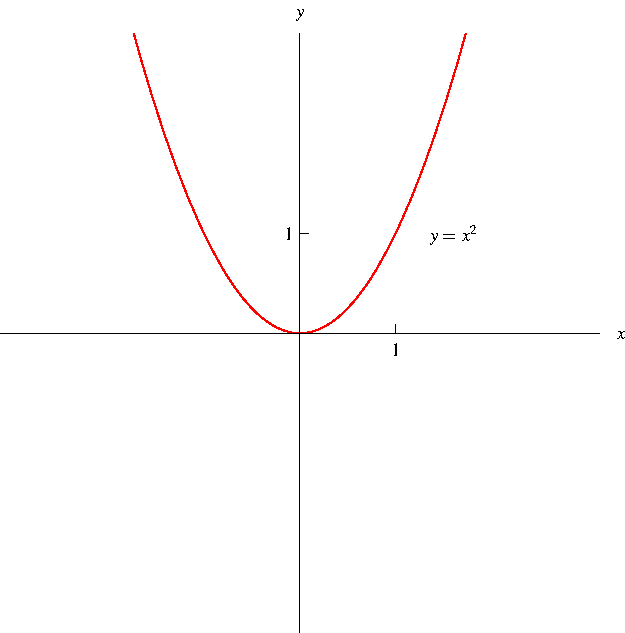
\includegraphics[height=4cm]{precalculus/pictures/01-02-xsquared.pdf}%
%}%
%\only<handout:4| 4>{%
%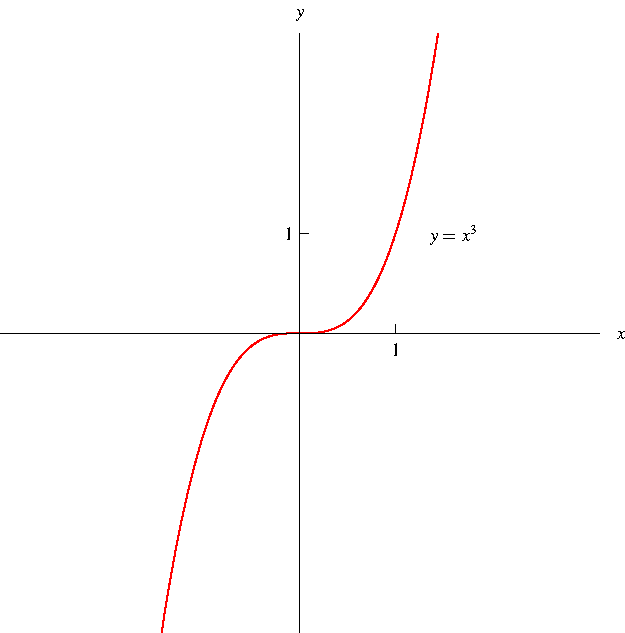
\includegraphics[height=4cm]{precalculus/pictures/01-02-xcubed.pdf}%
%}%
%\only<handout:5| 5>{%
%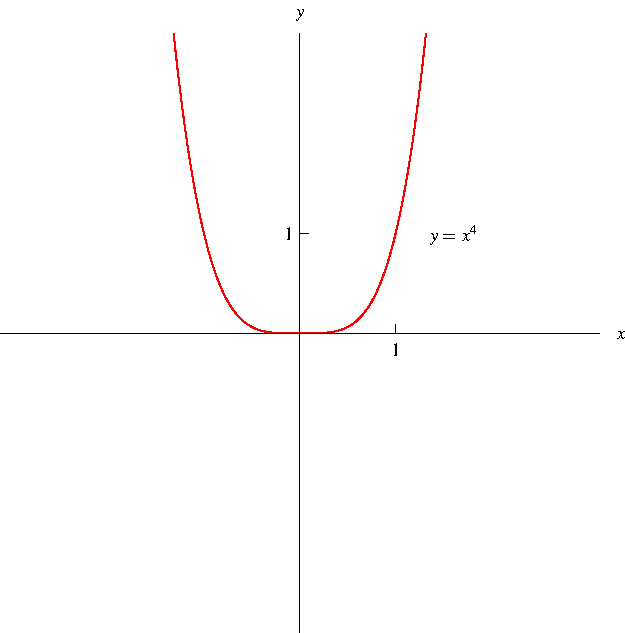
\includegraphics[height=4cm]{precalculus/pictures/01-02-xfourth.pdf}%
%}%
%\only<handout:6| 6>{%
%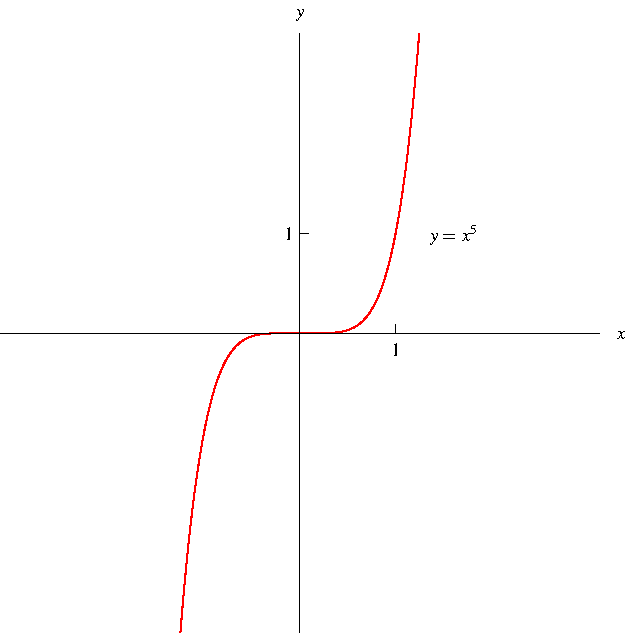
\includegraphics[height=4cm]{precalculus/pictures/01-02-xfifth.pdf}
%}%
}
\end{frame}
% end module power-functions-def

% begin module root-functions
\begin{frame}
\begin{itemize}
\item<1->  If $n$ is a positive integer, the function $f(x) = x^{\frac{1}{n}} = \sqrt[n]{x}$ is called a root function.
\item<2->  When $n = 2$, it is the square root function $f(x) = \sqrt{x}$.
\item<3->  The square root is not defined for negative numbers, so its domain is $[0, \infty)$.
\item<4->  Its graph is the top half of the parabola $x = y^2$.
\item<5->  The graph of the cube root function $f(x) = \sqrt[3]{x}$ is similar to that of the square root, but it is defined everywhere.
\end{itemize}
\begin{tabular}{cc}
\uncover<2->{%
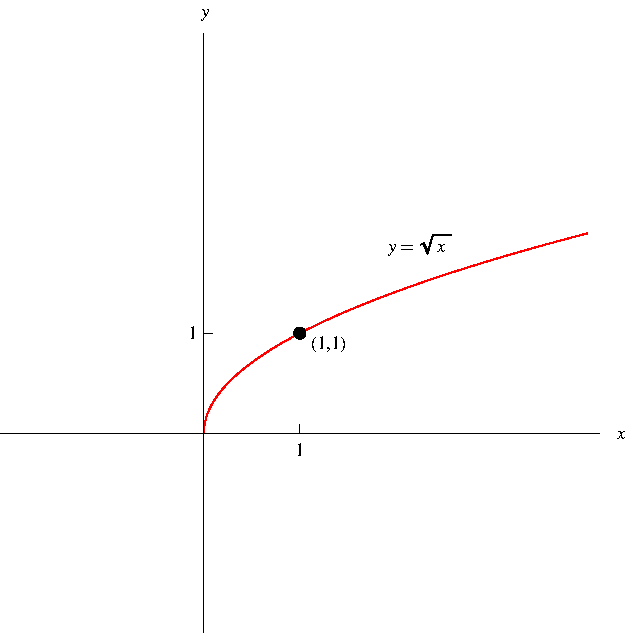
\includegraphics[height=3.5cm]{precalculus/pictures/01-02-sqrtx.pdf}%
}%
&%
\uncover<5->{%
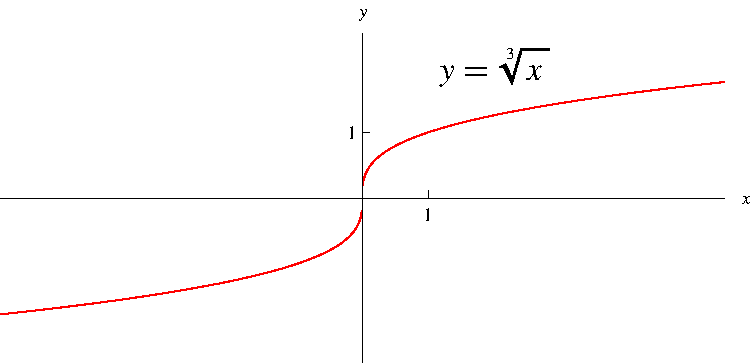
\includegraphics[height=3.5cm]{precalculus/pictures/cube-root.pdf}%
}%
\end{tabular}
\end{frame}
% end module root-functions

% begin module reciprocal-function
\begin{frame}
$f(x) = x^{-1} = \frac{1}{x}$ is called the reciprocal function.  Its graph has equation $y = \frac{1}{x}$, or $xy = 1$, and is an hyperbola with the coordinate axes as its asymptotes.
%\begin{center}%center does not work with well with pstricks and pgflayout.
\hfil\hfil\psset{xunit=0.6cm, yunit=0.6cm}
\begin{pspicture}(-5, -5)(5,5)
\psframe*[linecolor=white](-5,-5)(5,5)
\psaxes[ticks=none, labels=none]{<->}(0,0)(-5,-5)(5,5)\tiny
%Function formula: (1)/(x)
\rput(1,3){$y=\frac 1 x$}
\psplot[linecolor=red, plotpoints=1000]{0.2}{5}{1 x div } %Function formula: (1)/(x)
\rput(1,3){$y=\frac 1 x$}
\psplot[linecolor=red, plotpoints=1000]{-5}{-0.2}{1 x div }
\fcLabels{4.5}{4.5}
\end{pspicture}
%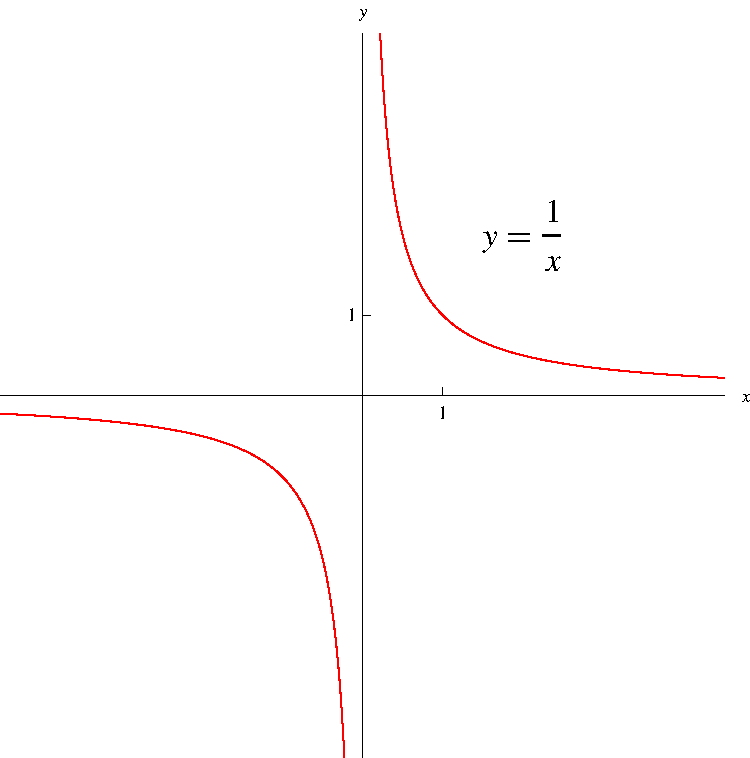
\includegraphics[height=5cm]{precalculus/pictures/reciprocal-function.pdf}%
%\end{center}
\end{frame}
% end module reciprocal-function

\subsection{Rational Functions}
% begin module rational-functions
\begin{frame}
\frametitle{Rational Functions}
\begin{definition}[Rational Function]
A rational function is a quotient of two polynomials; that is, a function of the form
\[
f(x) = \frac{g(x)}{h(x)},
\]
where $g$ and $h$ are polynomials.
\end{definition}
\begin{columns}[c]
\column{.4\textwidth}
\uncover<2->{
\psset{xunit=0.4cm, yunit=0.4cm}
\begin{pspicture}(-5, -5)(5,5) 
\psframe*[linecolor=white](-5,-5)(5,5) 
\psaxes[ticks=none, labels=none]{<->}(0,0)(-4.5,-4.5)(4.5,4.5)\tiny
%Function formula: \frac{x}{(x)^{2}-1} 
\rput(2.5,-3){$y=\frac{x}{x^{2}-1}$} 
\psplot[linecolor=red, plotpoints=1000]{1.11727}{4.5}{x -1 x 2 exp add div } %Function formula: \frac{x}{(x)^{2}-1} 
\psplot[linecolor=red, plotpoints=1000]{-0.895043}{0.895043}{x -1 x 2 exp add div } %Function formula: \frac{x}{(x)^{2}-1} 
\psplot[linecolor=red, plotpoints=1000]{-4.5}{-1.11727}{x -1 x 2 exp add div }
\psLabels{4.5}{4.5}
\end{pspicture} 
%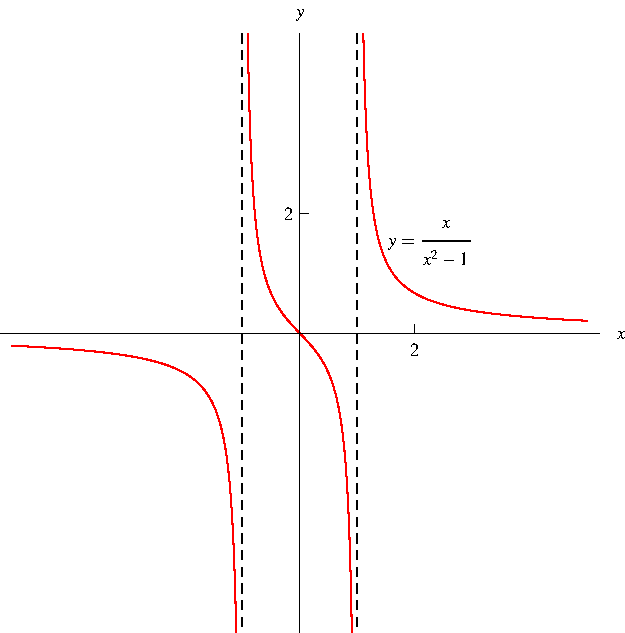
\includegraphics[height=4cm]{precalculus/pictures/01-02-rational.pdf}%
}
\column{.6\textwidth}
\uncover<2->{
\begin{example}[$x/(x^2-1)$]
The function
\[
f(x) = \frac{x}{x^2-1}
\]
is a rational function.
\end{example}
}
\end{columns}
\end{frame}
% end module rational-functions

\subsection{Algebraic Functions}
%Old Version from Greg. Greg, this slide is changed substantially, please take a look.
%% begin module algebraic-functions
%\begin{frame}
%\frametitle{Algebraic Functions}
%\begin{definition}[Algebraic Function]
%An algebraic function is a function that can be constructed using algebraic operations (such as addition, subtraction, multiplication, division, and taking roots) starting from polynomials.
%\end{definition}
%\uncover<2->{
%Algebraic functions can look pretty funny.
%\begin{tabular}{ccc}
%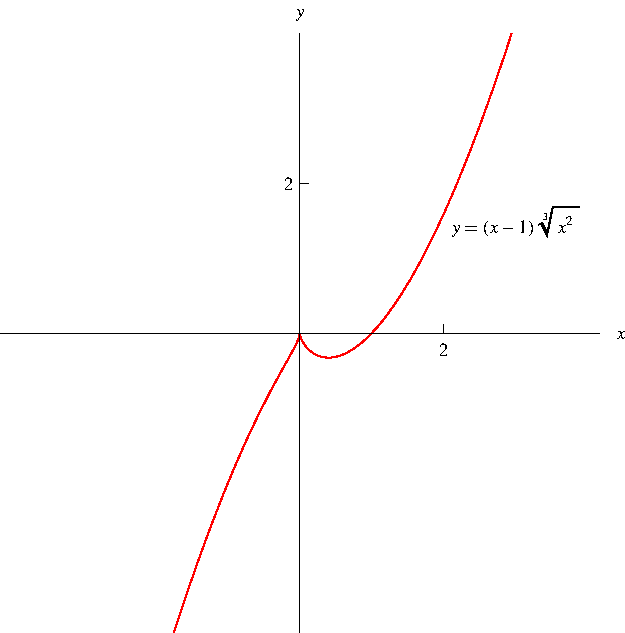
\includegraphics[height=3.8cm]{precalculus/pictures/01-02-algebraic1.pdf}&%
%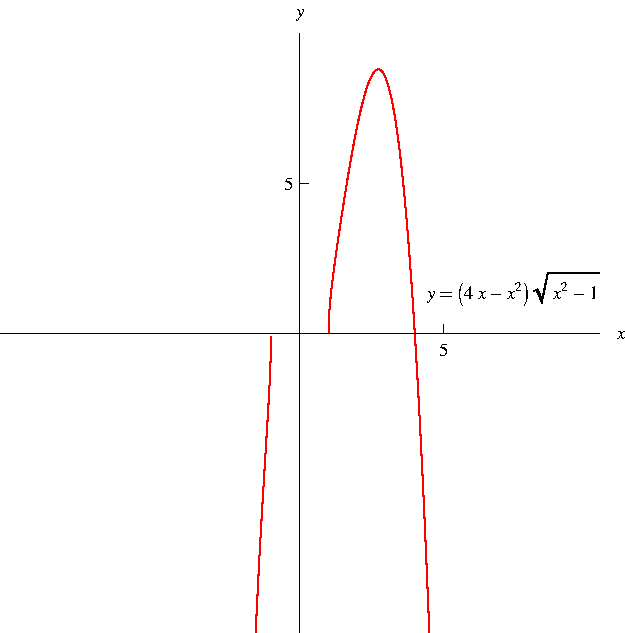
\includegraphics[height=3.8cm]{precalculus/pictures/01-02-algebraic2.pdf}&%
%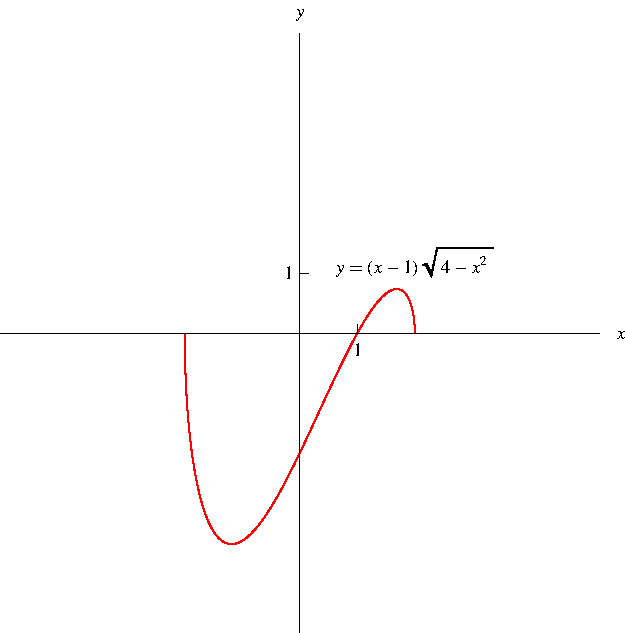
\includegraphics[height=3.8cm]{precalculus/pictures/01-02-algebraic3.pdf}%
%\end{tabular}
%}
%\end{frame}
%% end module algebraic-functions


% begin module algebraic-functions
\begin{frame}
\frametitle{Algebraic Functions}
\begin{definition}[Algebraic Function]
A function in $x$ that can be constructed using $x$, constants, and finitely many of the operations $+, -, *, /,$ and $\sqrt[n]{~}$ is an algebraic function.

\uncover<2->{{\footnotesize Outside of Calculus I: function $f(x)$ = algebraic if it satisfies a polynomial equation with polynomial coefficients, i.e., $a_0(x) +a_1(x)f(x)+\dots +a_n(x) \left(f(x)\right)^n=0$ for some polynomials  $a_i(x)$.}}
\end{definition}
\uncover<3->{
Examples.

\begin{tabular}{ccc}
\psset{xunit=0.3cm, yunit=0.3cm}
\begin{pspicture}(-5, -5)(5,5)
\tiny\psframe*[linecolor=white](-5,-5)(5,5)
\psaxes[ticks=none, labels=none]{<->}(0,0)(-4.5,-4.5)(4.5,4.5)\tiny
%Function formula: - ((- (x))^{5/3})- ((- (x))^{2/3})
\psplot[linecolor=red, plotpoints=1000]{-2}{-0.001}{x -1 mul 0.666667 exp -1 mul x -1 mul 1.66667 exp -1 mul add } %Function formula: (x)^{5/3}- ((x)^{2/3})
\rput[t](1,-5){$y=(x-1)\sqrt[3]{x^2}$}
\psplot[linecolor=red, plotpoints=1000]{0.001}{3}{x 0.666667 exp -1 mul x 1.66667 exp add }
\fcLabels{4.5}{4.5}
\end{pspicture}
%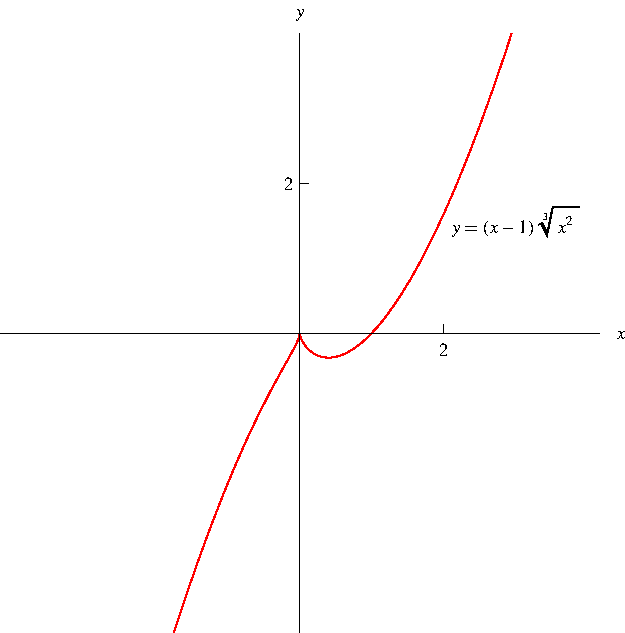
\includegraphics[height=3.8cm]{precalculus/pictures/01-02-algebraic1.pdf}
&%
\psset{xunit=0.3cm, yunit=0.3cm}
\begin{pspicture}(-5, -5)(5,5)
\tiny\psframe*[linecolor=white](-5,-5)(5,5)
\psaxes[ticks=none, labels=none]{<->}(0,0)(-4.5,-4.5)(4.5,4.5)\tiny
\psplot[linecolor=red, plotpoints=1000]{1}{5}{-1 x 2 exp add 0.5 exp x 2 exp mul -0.2 mul -1 x 2 exp add 0.5 exp x mul 0.8 mul add } %Function formula: 4/5 ((x) (((x)^{2}-1)^{1/2}))-1/5 (((x)^{2}) (((x)^{2}-1)^{1/2}))
\rput[t](1,-5){$y=\frac15(4x-x^2)\sqrt{x^2-1}$}
\psplot[linecolor=red, plotpoints=1000]{-2}{-1}{-1 x 2 exp add 0.5 exp x 2 exp mul -0.2 mul -1 x 2 exp add 0.5 exp x mul 0.8 mul add }
\fcLabels{4.5}{4.5}
\end{pspicture}
%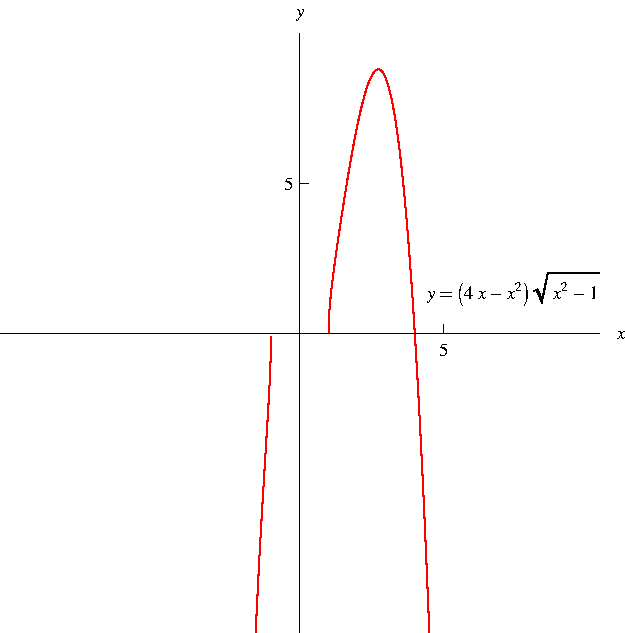
\includegraphics[height=3.8cm]{precalculus/pictures/01-02-algebraic2.pdf}
&%
\psset{xunit=0.3cm, yunit=0.3cm}
\begin{pspicture}(-5, -5)(5,5)
\tiny\psframe*[linecolor=white](-5,-5)(5,5)
\psaxes[ticks=none, labels=none]{<->}(0,0)(-4.5,-4.5)(4.5,4.5)\tiny
%Function formula: - ((4- ((x)^{2}))^{1/2})+(x) ((4- ((x)^{2}))^{1/2})
\rput[t](1,-5){$y=(x-1)\sqrt{4-x^2}$}
\psplot[linecolor=red, plotpoints=1000]{-2}{2}{x 2 exp -1 mul 4 add 0.5 exp x mul x 2 exp -1 mul 4 add 0.5 exp -1 mul add }
\fcLabels{4.5}{4.5}
\end{pspicture}
%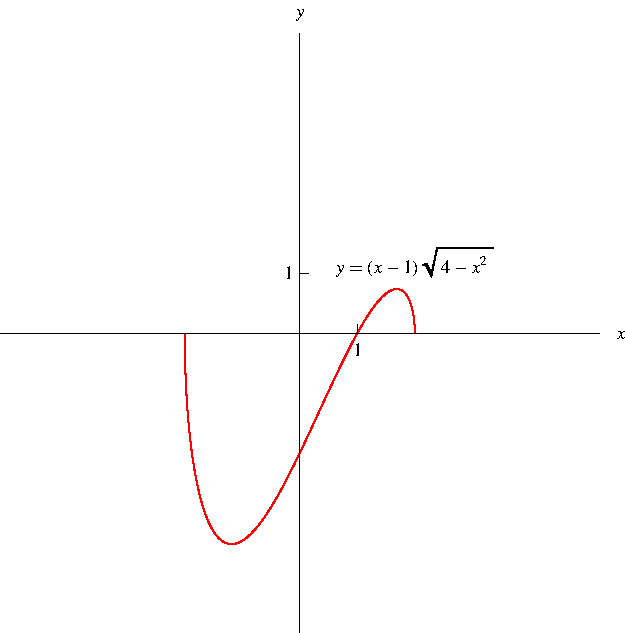
\includegraphics[height=3.8cm]{precalculus/pictures/01-02-algebraic3.pdf}
%
\end{tabular}
}
\end{frame}
% end module algebraic-functions

\subsection{Transcendental Functions}
% begin module transcendental-functions
\begin{frame}
\frametitle{Transcendental Functions}
Transcendental functions include many classes of functions.
\begin{itemize}
\item<2->  Trigonometric functions such as $\cos x, \sin x, \tan x,$ etc.
\item<3->  Exponential functions such as $2^x, \left( \frac{1}{2}\right)^x, 5^x, e^x$, etc.
\item<4->  The logarithm function $\ln x$.
\item<5->  And many more.
\item<6-> Outside of Calculus I: by definition, a function is transcendental if it is not algebraic, i.e., if it satisfies no polynomial equation.
\end{itemize}
\end{frame}
% end module transcendental-functions 

\section{1.3 New Functions from Old Functions}
\subsection{Transformations of Functions}
% begin module transformations-shifts
\begin{frame}
\frametitle{Transformations of Functions}
\begin{columns}[c]
\column{.5\textwidth}

\psset{xunit=1cm, yunit=1cm}
\begin{pspicture}(-0.5, -0.5)(4.7,4.7)%
\tiny%
\psframe*[linecolor=white](-5,-5)(5,5)%
\psaxes[ticks=none, labels=none]{<->}(0,0)(-0.5,-0.5)(5,4.5)%
\rput[t](5, -0.1){$x$}%
\rput[r](-0.1, 4.5){$y$}%
%\frac{1}{3} (3 x-6)^{3}-\frac{1}{3} (3 x-6)^{2}-\frac{1}{3} x+\frac{8}{3} 
\newcommand{\theFun}{3 x mul 6 sub dup dup mul mul 3 div 3 x mul 6 sub dup mul -3 div x -3 div 8 3 div add add add\space}%
\only<handout:0| -2>{%
\psplot[linecolor=red, plotpoints=1000]{1.65}{2.55}{\theFun}%
\rput[b] (2.55, 2.40654){\alert<-2>{$y=f(x)$}}%
}%
\only<handout:1| 3->{%
\psplot[linecolor=blue, plotpoints=1000]{1.65}{2.55}{\theFun}%
\rput[b] (2.55, 2.40654){$y=f(x)$}%
}%
\only<handout:0| 3>{%
\psplot[linecolor=red, plotpoints=1000]{1.65}{2.55}{\theFun 1.5 add }%
\rput[b](2.55, 3.90654){\alert<3>{$y=f(x)+c$}}%
}%
\only<handout:1| 4,5,22->{%
\psplot[linecolor=blue, plotpoints=1000]{1.65}{2.55}{\theFun 1.5 add }%
\rput[b](2.55, 3.90654){$y=f(x)+c$}%
}%
\only<handout:0| 4>{%
\psplot[linecolor=red, plotpoints=1000]{1.65}{2.55}{\theFun 1.5 sub}%
\rput[b](2.55, 0.906542){$y=f(x)-c$}%
}%
\only<handout:1| 5,22->{%
\psplot[linecolor=blue, plotpoints=1000]{1.65}{2.55}{\theFun 1.5 sub}%
\rput[b](2.55, 0.906542){$y=f(x)-c$}%
}%
\only<handout:0| 19>{%
\psplot[linecolor=red, plotpoints=1000]{3.15}{4.05}{1 dict begin /x x 1.5 sub def \theFun end}%
}%
\only<handout:1| 20,22->{%
\psplot[linecolor=blue, plotpoints=1000]{3.15}{4.05}{1 dict begin /x x 1.5 sub def \theFun end}%
\rput[b](4.05, 2.40654){$\alert<20>{y=f(x-c)}$}%
}%
\newcommand{\theAnimation}[6]{%
\uncover<handout:0|####1>{%
\fcXTickWithLabel{\curPt}{$x$}%
}%
\uncover<handout:0|####2>{%
\fcXTickWithLabel{\curPt 1.5 sub}{$x-c$}%
}%
\uncover<handout:0|####3>{%
\rput[l](! \curPt 1.5 sub 0.1 add 1 dict begin /x \curPt 1.5 sub def \theFun  end 2 div){$f(x-c)$}%
}%
\uncover<handout:0|####4>{%
\psline[linecolor=red, linewidth=2pt](! \curPt 1.5 sub 0)(! \curPt 1.5 sub 1 dict begin /x \curPt 1.5 sub def \theFun  end)%
}%
\uncover<handout:0|####5>{%
\rput[l](! \curPt 0.1 add 1 dict begin /x \curPt 1.5 sub def \theFun  end 2 div){$f(x-c)$}%
}%
\uncover<handout:0|####6>{%
\psline[linecolor=red, linewidth=2pt](! \curPt 0)(! \curPt 1 dict begin /x \curPt 1.5 sub def \theFun  end)%
}%
}%
\newcommand{\curPt}{3.3\space}%
\theAnimation{7-10}{8-10}{9-10}{9-19}{10}{10-19}%
\renewcommand{\curPt}{3.5\space}%
\theAnimation{11-14}{12-14}{13-14}{13-19}{14}{14-19}%
\renewcommand{\curPt}{3.8\space}%
\theAnimation{15-19}{16-19}{17-18}{17-19}{18}{18-19}%
%

\only<handout:0|21>{%
\psplot[linecolor=red, plotpoints=1000]{0.15}{1.05}{1 dict begin /x x 1.5 add def \theFun end}
\rput[b](1.05, 2.40654){\alert<6>{$y=f(x+c)$}}
}
\only<handout:1|22->{%
\psplot[linecolor=blue, plotpoints=1000]{0.15}{1.05}{1 dict begin /x x 1.5 add def \theFun end}
\rput[b](1.05, 2.40654){$y=f(x+c)$}
}
\end{pspicture}
%\ \only<handout:0| -2>{%
%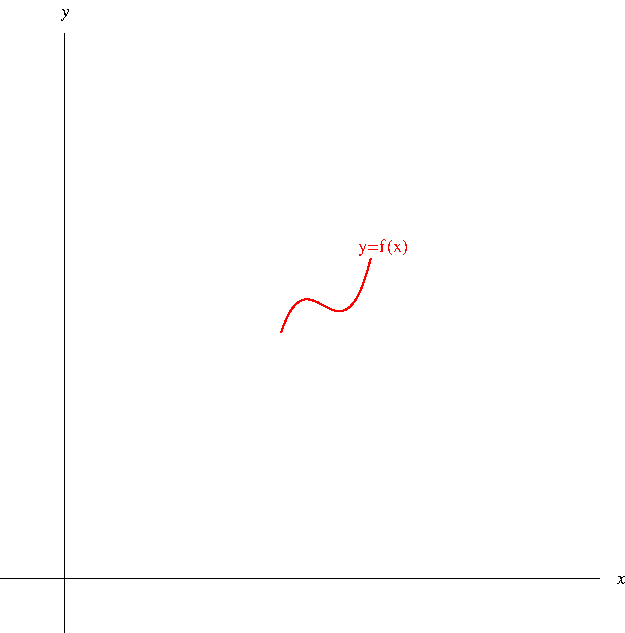
\includegraphics[height=5cm]{precalculus/pictures/01-03-shifta.pdf}%
%}%
%\only<handout:0| 3>{%
%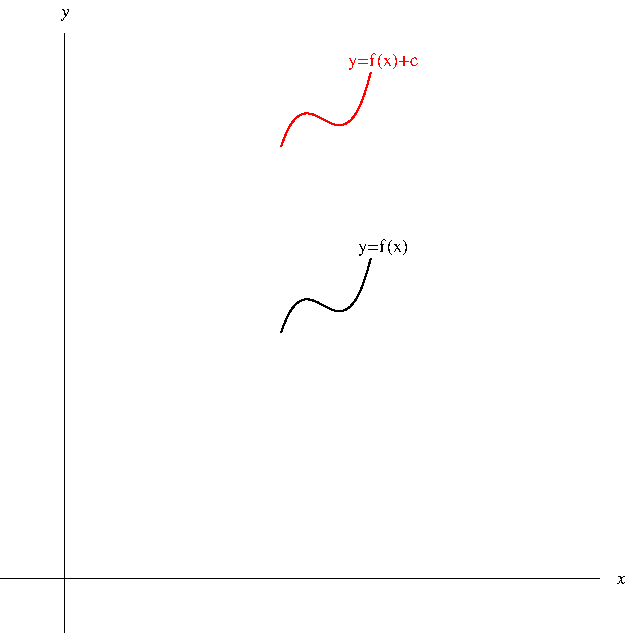
\includegraphics[height=5cm]{precalculus/pictures/01-03-shiftb.pdf}%
%}%
%\only<handout:0| 4>{%
%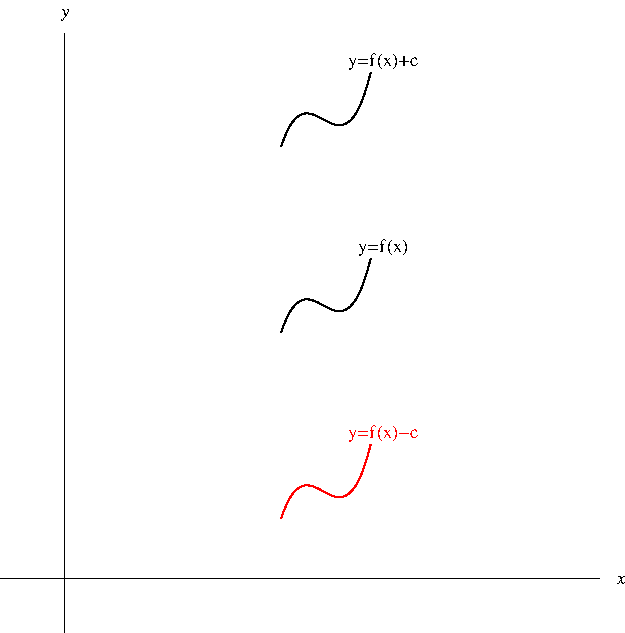
\includegraphics[height=5cm]{precalculus/pictures/01-03-shiftc.pdf}%
%}%
%\only<handout:0| 5>{%
%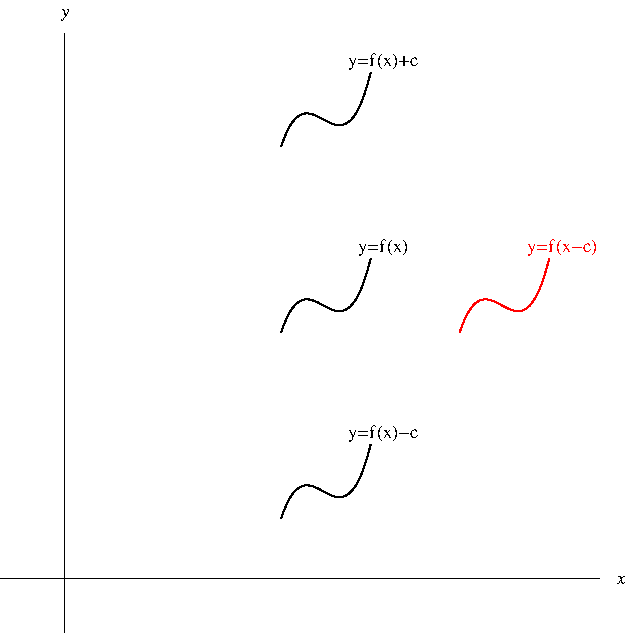
\includegraphics[height=5cm]{precalculus/pictures/01-03-shiftd.pdf}%
%}%
%\only<6>{%
%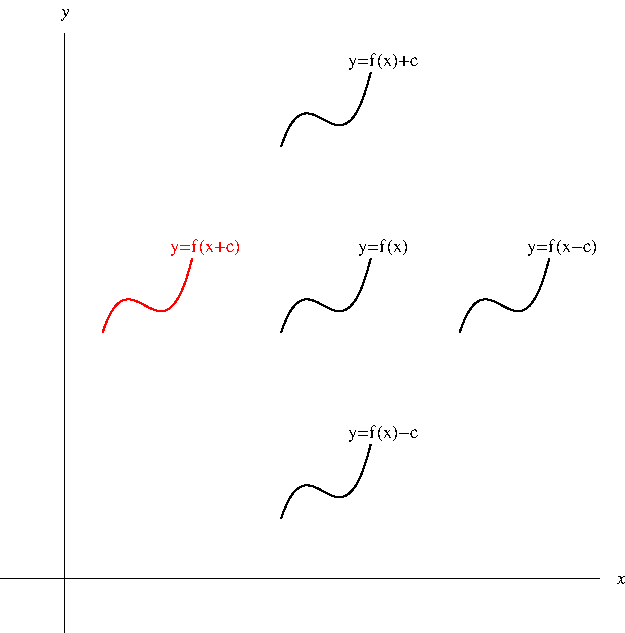
\includegraphics[height=5cm]{precalculus/pictures/01-03-shifte.pdf}%
%}%a
\column{.5\textwidth}
\begin{itemize}
\item What happens to the graph if we add/subtract a positive constant $c$ in the equation of a function $f$?
\item What happens if we add or subtract $c$ from $x$ before applying the function $f$?
\end{itemize}
\end{columns}

\uncover<2->{
\begin{tabular}{|l|l|}
\hline
\alertNoH{ 3}{$f(x)+c$} &%
\uncover<3->{\alertNoH{3,22}{Shift the graph of $f(x)$ $c$ units up.}} \\%
\alertNoH{ 4}{$f(x)-c$} &%
\uncover<4->{\alertNoH{4,22}{Shift the graph of $f(x)$ $c$ units down.}} \\%
\alertNoH{6}{$f(x-c)$} &%
\uncover<6->{\alertNoH{6,22}{Shift the graph of $f(x)$ \fcAnswerUncover{6}{20}{$c$ units right}.}} \\%
\alertNoH{21}{$f(x+c)$} &%
\uncover<21->{\alertNoH{21,22}{Shift the graph of $f(x)$ $c$ units left.}}\\%
\hline
\end{tabular}

}
\end{frame}
% end module transformations-shifts

% begin module transformations-shifts-example
\begin{frame}
\begin{example}
Draw a graph of the function $f(x) = x^2 + 6x + 10$.
\begin{columns}[c]
\column{.5\textwidth}

\psset{xunit=0.7cm, yunit=0.7cm}
\begin{pspicture}(-5.1, -0.6)(3.1,5.1)
\tiny
\fcAxesStandard{-5.03}{-0.5}{3}{5}
\rput[rt](-0.1,-0.1){$(0,0)$}
\fcFullDot{0}{0}
%Function formula: (-3+x)^{2}-9+6 (x)
\only<handout:0| 7>{
\rput(2.5,2){$y=x^2$}
\psplot[linecolor=red, plotpoints=1000]{-2.23607}{2.23607}{x 6 mul -9 x -3 add 2 exp add add } %Function formula: (x)^{2}+10+6 (x)
}
\only<handout:1| 8->{
\rput(2.5,2){\color{gray}$y=x^2$}
\psplot[linecolor=gray, plotpoints=1000]{-2.23607}{2.23607}{x 6 mul -9 x -3 add 2 exp add add } %Function formula: (x)^{2}+10+6 (x)
\rput[rt](-3.1,0.9){$(-3,1)$}
\psline{->}(0,0)(-3,1)
\fcFullDot{-3}{1}

\rput[b](-3,4.2){\alert<8->{$y=x^{2}+6x+10$}}
\psplot[linecolor=red, plotpoints=1000]{-5}{-1}{x 6 mul 10 x 2 exp add add }
}
\end{pspicture}

\column{.5\textwidth}
\uncover<2->{
Complete the square:
}
\begin{eqnarray*}
\uncover<3->{f(x)} & \uncover<3->{ = } & \uncover<3->{x^2 + 6x + 10} \\
& \uncover<4->{ = } & \uncover<4->{(x^2 + 6x \uncover<5->{\alert<handout:0| 5>{+ 9}}) + 10 \uncover<5->{\alert<handout:0| 5>{- 9}}} \\
 & \uncover<6->{ = } & \uncover<6->{(x + 3)^2 + 1} \\
\end{eqnarray*}
\end{columns}
\uncover<7-8>{}
\end{example}
\end{frame}
% end module transformations-shifts-example

% begin module transformations-magnifications
\begin{frame}
\begin{columns}[c]
\column{.5\textwidth}

\psset{xunit=0.7cm, yunit=0.7cm}
\begin{pspicture}(-4, -3.5)(4.5,5)
\tiny
\fcAxesStandard{-4}{-3.5}{4.5}{5}
%Function formula: 10/3+1/3 ((-3+3 (x))^{3})-1/3 ((-3+3 (x))^{2})-1/3 (x)
\only<handout:1| 1->{
\psplot[linecolor=red, plotpoints=1000]{1.65}{2.55}{x -0.333333 mul x 3 mul -6 add 2 exp -0.333333 mul x 3 mul -6 add 3 exp 0.333333 mul 2.66667 add add add }
\rput[b] (2.55, 2.40654){$y=f(x)$}
}
%\only<handout:0| 3->{
%\psplot[linecolor=blue, plotpoints=1000]{1.65}{2.55}{x -0.333333 mul x 3 mul %-6 add 2 exp -0.333333 mul x 3 mul -6 add 3 exp 0.333333 mul 2.66667 add add %add }
%\rput[b] (2.55, 2.40654){$y=f(x)$}
%}

\only<handout:0| 3>{
\psplot[linecolor=red, plotpoints=1000]{1.65}{2.55}{x -0.333333 mul x 3 mul -6 add 2 exp -0.333333 mul x 3 mul -6 add 3 exp 0.333333 mul 2.66667 add add add 2 mul}
\rput[b] (2.55, 4.80654){{$y=cf(x)$}}
}
\only<handout:1| 4->{
\psplot[linecolor=blue, plotpoints=1000]{1.65}{2.55}{x -0.333333 mul x 3 mul -6 add 2 exp -0.333333 mul x 3 mul -6 add 3 exp 0.333333 mul 2.66667 add add add 2 mul}
\rput[b] (2.55, 4.80654){$y=cf(x)$}
}

\only<handout:0| 4>{
\psplot[linecolor=red, plotpoints=1000]{1.65}{2.55}{x -0.333333 mul x 3 mul -6 add 2 exp -0.333333 mul x 3 mul -6 add 3 exp 0.333333 mul 2.66667 add add add 2 div}
\rput[b] (2.55, 0.40654){{$y=\frac{1}{c}f(x)$}}
}
\only<handout:1| 5->{
\psplot[linecolor=blue, plotpoints=1000]{1.65}{2.55}{x -0.333333 mul x 3 mul -6 add 2 exp -0.333333 mul x 3 mul -6 add 3 exp 0.333333 mul 2.66667 add add add 2 div}
\rput[b] (2.55, 0.40654){$y=\frac{1}{c}f(x)$}
}

\only<handout:0| 5>{
\psplot[linecolor=red, plotpoints=1000]{1.65}{2.55}{x -0.333333 mul x 3 mul -6 add 2 exp -0.333333 mul x 3 mul -6 add 3 exp 0.333333 mul 2.66667 add add add -1 mul}
\rput[t] (2.55, -2.40654){{$y=-f(x)$}}
}
\only<handout:1| 6->{
\psplot[linecolor=blue, plotpoints=1000]{1.65}{2.55}{x -0.333333 mul x 3 mul -6 add 2 exp -0.333333 mul x 3 mul -6 add 3 exp 0.333333 mul 2.66667 add add add -1 mul}
\rput[t] (2.55, -2.40654){$y=-f(x)$}
}

\only<handout:0| 6>{
%Function formula: 8/3+1/3 ((-6-3 (x))^{3})+1/3 (x)-1/3 ((-6-3 (x))^{2})
\psplot[linecolor=red, plotpoints=1000]{-2.55}{-1.65}{x -3 mul -6 add 2 exp -0.333333 mul x 0.333333 mul x -3 mul -6 add 3 exp 0.333333 mul 2.66667 add add add }
\rput[b] (-2.55, 2.40654){{$y=f(-x)$}}
}
\only<handout:1| 7->{
%Function formula: 8/3+1/3 ((-6-3 (x))^{3})+1/3 (x)-1/3 ((-6-3 (x))^{2})
\psplot[linecolor=blue, plotpoints=1000]{-2.55}{-1.65}{x -3 mul -6 add 2 exp -0.333333 mul x 0.333333 mul x -3 mul -6 add 3 exp 0.333333 mul 2.66667 add add add }
\rput[b] (-2.55, 2.40654){$y=f(-x)$}
}
\end{pspicture}
%\ \only<handout:0| -2>{%
%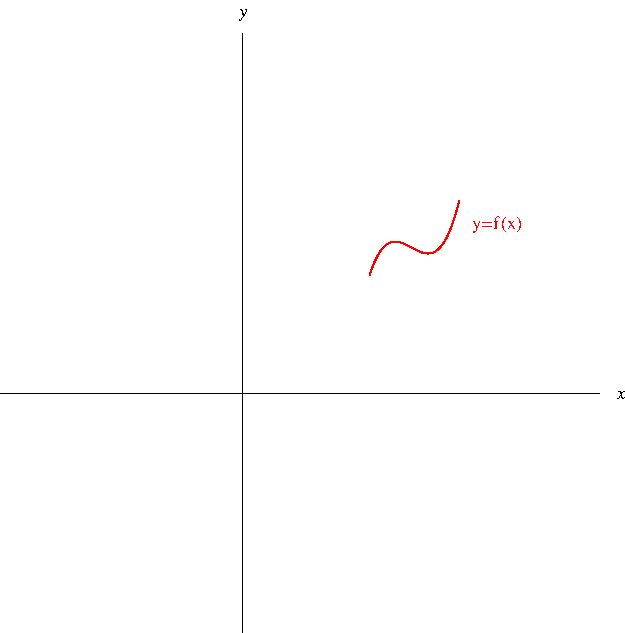
\includegraphics[height=5cm]{precalculus/pictures/01-03-maga.pdf}%
%}%
%\only<handout:0| 3>{%
%\includegraphics[height=5cm]{precalculus/pictures/01-03-magb.pdf}%
%}%
%\only<handout:0| 4>{%
%\includegraphics[height=5cm]{precalculus/pictures/01-03-magc.pdf}%
%}%
%\only<handout:0| 5>{%
%\includegraphics[height=5cm]{precalculus/pictures/01-03-magd.pdf}%
%}%
%\only<6>{%
%\includegraphics[height=5cm]{precalculus/pictures/01-03-mage.pdf}%
%}%

\column{.5\textwidth}
\alertNoH{3-4}{What happens if we multiply or divide by a constant $c > 1$ in the equation of a function $f$?}  \alertNoH{5}{What happens if we multiply $f$ by $-1$?}  \alertNoH{6}{What happens if we multiply $x$ by $-1$ before applying $f$?}
\end{columns}

\begin{tabular}{|l|l|}
\hline
\alert<handout:0| 3>{$cf(x)$} &%
\uncover<3->{\alert<handout:0| 3>{Stretch the graph of $f(x)$ vertically by a factor of $c$.}} \\%
\alert<handout:0| 4>{$(1/c)f(x)$} &%
\uncover<4->{\alert<handout:0| 4>{Compress the graph of $f(x)$ vertically by a factor of $c$.}} \\%
\alert<handout:0| 5>{$-f(x)$} &%
\uncover<5->{\alert<handout:0| 5>{Reflect the graph of $f(x)$ in the $x$-axis.}} \\%
\alert<handout:0| 6>{$f(-x)$} &%
\uncover<6->{\alert<handout:0| 6>{Reflect the graph of $f(x)$ in the $y$-axis.}}\\%
\hline
\end{tabular}
\uncover<7>{~} %this line is needed to avoid a latexing bug: without this line, the next slide will be messed up.

\end{frame}
% end module transformations-magnifications

% begin module transformations-horizontal-stretches
\begin{frame}\ %
\uncover<1->{}
\psset{xunit=1.4cm, yunit=1.4cm}
\begin{pspicture}(-0.6, -1.4)(6.2,1.4) 
\psaxesStandard{-0.6}{-1.4}{6.2}{1.4}

%Function formula: sin{}(x) 
\rput[t](4.71238898, -1.1){\alert<1-2>{$y=sin{}(x)$}} 

\uncover<1-2>{
\psplot[linecolor=red, plotpoints=1000]{-0.5}{6}{x 57.29578 mul sin }
}
\uncover<3->{
\psplot[linecolor=blue, plotpoints=1000]{-0.5}{6}{x 57.29578 mul sin }
}

\psline(1.570796327, -0.05)(1.570796327, 0.05)
\rput[t](1.570796327, -0.1) {$\frac{\pi}{2}$}

\psline(3.141592654, -0.05)(3.141592654, 0.05)
\rput[t](3.141592654, -0.1) {$\pi$}


\uncover<3->{
 %Function formula: sin{}(3/2 (x)) 
\uncover<3>{
\psplot[linecolor=red, plotpoints=1000]{-0.5}{6}{x 1.5 mul 57.29578 mul sin } 
}
\uncover<4->{
\psplot[linecolor=blue, plotpoints=1000]{-0.5}{6}{x 1.5 mul 57.29578 mul sin } 
}
\rput(3.141592654, -1.1){\alert<3>{$y=\sin{}(cx)$}} 

\psline(1.047197551, -0.05)(1.047197551, 0.05)
\rput[t](1.047197551, -0.1) {$\frac{\pi}{2c}$}

\psline(2.094395102, -0.05)(2.094395102, 0.05)
\rput[t](2.094395102, -0.1) {$\frac{\pi}{c}$}

}
\uncover<4->{
\rput[b](3.14,1.1){\alert<4>{$y=\sin\left(\frac{x}{c}\right)$}} 
\psplot[linecolor=red, plotpoints=1000]{-0.5}{6}{x 0.666667 mul 57.29578 mul sin } 

\psline(2.35619449, -0.05)(2.35619449, 0.05)
\rput[t](2.35619449, -0.1) {$\frac{\pi c}{2}$}

\psline(4.71238898, -0.05)(4.71238898, 0.05)
\rput[t](4.71238898, -0.1) {$\pi c$}
}
\end{pspicture} 
%\includegraphics[height=6cm]{precalculus/pictures/01-03-stretcha.pdf}%
%}%
%\only<handout:0| 3>{%
%\includegraphics[height=6cm]{precalculus/pictures/01-03-stretchb.pdf}%
%}%
%\only<4->{%
%\includegraphics[height=6cm]{precalculus/pictures/01-03-stretchc.pdf}%
%}%a

What happens if we multiply or divide $x$ by a constant $c > 1$ before applying $f$?

\uncover<2->{
\begin{tabular}{|l|l|}
\hline
\alert<handout:0| 3>{$f(cx)$} &%
\uncover<3->{\alert<handout:0| 3>{Compress the graph of $f(x)$ horizontally by a factor of $c$.}} \\%
\alert<handout:0| 4>{$f((1/c)x)$} &%
\uncover<4->{\alert<handout:0| 4>{Stretch the graph of $f(x)$ horizontally by a factor of $c$.}} \\%
\hline
\end{tabular}
}
\end{frame}
% end module transformations-horizontal-stretches
% begin module transformations-absolute-value
\begin{frame}
What happens when we take the absolute value of a function?
\uncover<2->{
\[
|f(x)| = \left\{ \begin{array}{rcc}
f(x) & \textrm{if} & f(x) \geq 0\\
-f(x) & \textrm{if} & f(x) < 0
\end{array}\right.
\]
}
\uncover<3->{%
This tells us how to draw the graph of $y = |f(x)|$: the part of the graph above the $x$-axis remains the same; the part below the $x$-axis is reflected about the $x$-axis.
}
\uncover<4->{
\begin{example}[Example 5, p. 41]
Draw the graph of the function $f(x) = |x^2 - 1|$.
\begin{columns}[c]
\column{.4\textwidth}
\ \only<handout:0| -4>{%
\includegraphics[height=4cm]{precalculus/pictures/01-03-ex5z.pdf}%
}%
\only<handout:0| 5>{%
\includegraphics[height=4cm]{precalculus/pictures/01-03-ex5a.pdf}%
}%
\only<handout:0| 6>{%
\includegraphics[height=4cm]{precalculus/pictures/01-03-ex5b.pdf}%
}%
\only<7->{%
\includegraphics[height=4cm]{precalculus/pictures/01-03-ex5c.pdf}%
}%
\column{.6\textwidth}
\begin{itemize}
\item<5->  Draw the graph of $f(x) = x^2 - 1$.
\item<6->  Identify the part(s) below the $x$-axis.
\item<7->  Flip those parts over the $x$-axis.
\end{itemize}
\end{columns}
\end{example}
}
\end{frame}
% end module transformations-absolute-value

\subsection{Combinations of Functions}
% begin module combinations-functions
\begin{frame}
\frametitle{Combinations of Functions}
Two functions $f$ and $g$ can be combined to form new functions $f+g$, $f-g$, $f\cdot g$, and $\frac{f}{g}$:
\[
\begin{array}{rcll|l}
\uncover<2->{\alertNoH{3} {(f+g)(x)}} &\uncover<2->{\alertNoH{3}{=} }&\uncover<3->{ \alertNoH{3}{f(x) + g(x)}}\\
\uncover<2->{\alertNoH{4,5}{(f-g)(x)}}&\uncover<2->{\alertNoH{4,5}{=}}&\fcAnswer{5}{ f(x)-g(x)} \\
\uncover<2->{\alertNoH{6,7} {(f\cdot g)(x) }}&\uncover<2->{\alertNoH{6,7}{=}}& \fcAnswer{7}{f(x) \cdot g(x)}\\
\uncover<2->{\alertNoH{8,9}{\left(\frac{f}{g}\right) (x)}}& \uncover<2->{\alertNoH{8,9}{=}}& \fcAnswer{9}{ \frac{f(x)}{\alertNoH{10}{g(x)}}}\uncover<9->{ && \alertNoH{10,21}{\text{for } g(x)\neq 0}\quad .}
\end{array}
\]
\uncover<11->{Let $\text{Dom}(f)$ denote the domain of $f$.} \uncover<13->{\alertNoH{14,15}{The function $f+g$ is defined only if both $f$ and $g$ are defined, and similarly for the others. }} \uncover<14->{\alertNoH{14}{Therefore}} 
\[
\begin{array}{@{}rcll|l}
\uncover<12->{\alertNoH{14,15}{\text{Dom}(f+g)}}&\uncover<12->{\alertNoH{13,14,15}=}&\fcAnswerUncover{12}{15}{ \text{Dom}(f)\alertNoH{16}{ \cap} \text{Dom}(g) } \uncover<15->{&&\alertNoH{16}{ \cap\text{ stands for} } } \\
\uncover<12->{\alertNoH{17,18}{\text{Dom}(f-g)}}&\uncover<12->{\alertNoH{17,18}{=}}&\fcAnswerUncover{12}{18}{ \text{Dom}(f)\cap \text{Dom}(g) } \uncover<15->{&&\alertNoH{16}{\text{set intersection}} }\\
\uncover<12->{\alertNoH{17,18}{ \text{Dom}(f\cdot g)}} &\uncover<12->{ \alertNoH{17,18}{=}} &\fcAnswerUncover{12}{18} { \text{Dom}(f)\cap \text{Dom}(g)}\\
\uncover<12->{\alertNoH{19,20}{ \text{Dom}\left(\frac{f}{g}\right)}} &\uncover<12->{\alertNoH{19,20}{=}}& \fcAnswerUncover{12}{20}{ \text{Dom}(f)\cap \text{Dom}(g) \cap\alertNoH{21}{ \alertNoH{22}{\{} x\alertNoH{23}{ \textbf{|} }\alertNoH{24}{ g(x)\neq 0} \alertNoH{22}{ \}}} } \uncover<21->{ &&\alertNoH{21}{ \begin{array}{@{}l}\text{right expr.} \\ \text{stands for \alertNoH{22}{set} } \\ \alertNoH{23}{\text{where }} \alertNoH{24}{g(x)\neq 0}\end{array}}} \\
\end{array}
\]

\end{frame}

% end module combinations-functions

% begin module composition-functions
\begin{frame}
\begin{definition}[Composition of $f$ and $g$]
If $f$ and $g$ are two functions, then the composition of $f$ and $g$ is written $f\circ g$ and is defined by the formula
\[
(f\circ g)(x) = f(g(x)).
\]
\end{definition}

Imagine $f$ and $g$ as machines taking some input and producing some output. Then $f\circ g$ corresponds to attaching both machines end-to-end so that the output of $g$ becomes the input of $f$.
\includegraphics[height=2cm]{precalculus/pictures/01-03-machines.pdf}%

\uncover<2->{
The domain of $f\circ g$ is the set of all numbers $x$ in the domain of $g$ such that $g(x)$ is in the domain of $f$.  If the domain of $f$ is $A$ and the domain of $g$ is $B$, we write this as
\[
\{ x\in B |\ g(x) \in A\} .
\]
}
\end{frame}
% end module composition-functions

% begin module composition-example
\begin{frame}
\begin{example}
Find $\alertNoH{2}{f\circ g},\alertNoH{14}{g\circ f}, \alertNoH{27}{g\circ g}$ and their domains, where \alertNoH{10,16}{$\alertNoH{5}{ f(} \alertNoH{6}{ x} \alertNoH{5}{) =}\only<handout:0|5> {\color{red}} \sqrt{\only<handout:0|5>{\color{black}} \alertNoH{6}{x}}$} and \alertNoH{4,29}{$\alertNoH{17,30}{ g(}\alertNoH{18,31}{ x} \alertNoH{17,30}{) = }\only<handout:0|17,30>{\color{red}} \sqrt{3 - \only<handout:0|17,30>{ \color{black}} \alertNoH{18,31}{x} }$}.

$
\begin{array}{rclll}
\only<handout:1|1-26>{%
\uncover<2->{\alertNoH{3}{ (\alertNoH{2}{f\circ g})(x)}} &\uncover<3->{ \alertNoH{3}{ =}} & \uncover<3->{\alertNoH{3}{ f(\alertNoH{4}{g(x)})}} \uncover<4->{ =\only<handout:0|5>{\color{red}} f\left( \only<handout:0|5>{ \color{black}}   \alertNoH{4,6}{\sqrt{3 - x}} \only<handout:0|5>{\color{red}} \right)} \uncover<5->{ = \only<handout:0|5>{ \color{red}}  \alertNoH{7}{\sqrt{ \only<handout:0|5>{ \color{black}} \alertNoH{6}{\sqrt{3-x}}}}} \uncover<7->{  \alertNoH{7}{= \sqrt[4]{\alertNoH{7,9}{ 3-x} }}}\\
\uncover<8->{\text{Domain: }}\\
\uncover<9->{\alertNoH{9}{\alertNoH{10}{3}-x}&\alertNoH{9}{\geq} & \alertNoH{9}{0}} \\
\uncover<10->{\alertNoH{11}{-}x&\alertNoH{11}{\geq} & \alertNoH{10}{ \alertNoH{11}{-} 3}}\\
\uncover<11->{\alertNoH{13}{x}&\alertNoH{11,13}{\leq}&\alertNoH{13}{ 3} }\\
\uncover<12->{\alertNoH{12,13}{x} &\alertNoH{12,13}{\in}& \fcAnswer{13}{(-\infty , 3].}}\\
\uncover<14->{\alertNoH{15}{ (\alertNoH{14}{g\circ f})(x)}}& \uncover<15->{ \alertNoH{15}{=} } & \uncover<15->{ \alertNoH{15}{ g(\alertNoH{16}{ f(x)})}}
\uncover<16->{ = \alertNoH{17}{g(}\alertNoH{16,18}{\sqrt{x}}\alertNoH{17}{)}} \uncover<17->{ = \only<handout:0|17>{\color{red}}  \sqrt{\alertNoH{21}{ 3 - \only<handout:0|17>{ \color{black}} \alertNoH{18}{\sqrt{\alertNoH{20}{x}} }} }}\\
\uncover<19->{\text{Domain}:}\\
\uncover<20->{\alertNoH{20,26}{x}&\alertNoH{20,26}{\geq} & \alertNoH{20,26}{0} }\\
\uncover<21->{\alertNoH{21}{\alertNoH{22}{ 3} - \sqrt{x}}& \alertNoH{21}{ \geq } & \alertNoH{21}{ 0} }\\
\uncover<22->{ \alertNoH{23}{-} \sqrt{x} &\alertNoH{23}{\geq }& \alertNoH{22}{ \alertNoH{23}{-}3 }}\\
\uncover<23->{\sqrt{x}&\alertNoH{23}{ \leq} & 3} \\
\uncover<24->{\alertNoH{26}{ x}& \alertNoH{26}{ \alertNoH{0}{\leq}} &\alertNoH{26}{ 9}}\\
\uncover<25->{ \alertNoH{25,26}{x}&\alertNoH{25,26}{\in}& \fcAnswer{26}{[0,9]}} \\
}%only<handout:1|1->
\only<handout:2|27->{%
\uncover<27->{\alertNoH{28}{ (\alertNoH{27}{g\circ g})(x)}} & \uncover<28->{ \alertNoH{28} {=} } & \uncover<28->{\alertNoH{28}{ g( \alertNoH{29 }{ g(x)})}} \uncover<29->{ = \only<handout:0|30>{\color{red}}  g \left( \only<handout:0|30>{ \color{black}} \alertNoH{29}{\sqrt{3 - x}}  \only<handout:0|30>{\color{red}} \right)}  \uncover<30->{ \only<handout:0|30>{\color{red}} = \sqrt{\alertNoH{36}{ 3 - \only<handout:0|30>{\color{black}}\alertNoH{31}{\sqrt{\alertNoH{33}{3-x} } }}}}\\
\uncover<32->{\text{Domain}:}\\
\uncover<33->{\alertNoH{33}{\alertNoH{34} {3}-x} & \alertNoH{33}{\geq} &\alertNoH{33}{ 0}}\\
\uncover<34->{\alertNoH{35}{-}x&\alertNoH{35}{\geq} & \alertNoH{34}{ \alertNoH{35}{ - } 3}}\\
\uncover<35->{\alertNoH{43}{x}&\alertNoH{35,43}{\leq} &\alertNoH{43}{ 3}}\\
\uncover<36->{\alertNoH{36}{\alertNoH{37}{3}-\sqrt{3-x}}&\alertNoH{36}{\geq }&\alertNoH{36}{ 0}} \\
\uncover<37->{\alertNoH{38}{-}\sqrt{3-x}&\alertNoH{38}{\geq}& \alertNoH{37}{\alertNoH{38}{-} 3}}\\
\uncover<38->{\sqrt{3-x}&\alertNoH{38}{\leq}& 3} \\
\uncover<39->{\alertNoH{40}{3}-x&\alertNoH{0}{\leq} &\alertNoH{40}{ 9}}\\
\uncover<40->{\alertNoH{41}{-}x&\alertNoH{41}{\leq}& \alertNoH{40}{6}}\\
\uncover<41->{\alertNoH{43}{x}&\alertNoH{41,43}{\geq}& \alertNoH{43}{ \alertNoH{41}{-}6} }\\
\uncover<42->{\alertNoH{42,43}{x}&\alertNoH{42,43}{\in}& \fcAnswer{43}{[-6 , 3].}}
}%only<handout:2|>
\end{array}
$

%\column{.2\textwidth}
%\begin{eqnarray*}
%& & f\circ f  \\
%& & \uncover<2->{(f\circ f)(x)}\\
%& \uncover<3->{ = } & \uncover<3->{f(\alertNoH{ 4}{f(x)})}\\
%& \uncover<4->{ = } & \uncover<4->{\alertNoH{ 5}{f(}\alertNoH{ 4-5}{\sqrt{x}}\alertNoH{ 5}{)}}\\
%& \uncover<5->{ = } & \uncover<5->{\alertNoH{ 5}{\sqrt{\sqrt{x}}}}\\
%& \uncover<6->{ = } & \uncover<6->{\alertNoH{ 5}{\sqrt[4]{x}}}\\
%\end{eqnarray*}
\end{example}

\vskip 10cm
\end{frame}
% end module composition-example

}% end lecture

\lect{Fall 2015}{Trigonometry}{3}{%begin lecture
%DesiredLectureName: Trigonometry
\section{Trigonometry}
\subsection{Angles}
\begin{frame}
 \frametitle{Angles}

$$\cos{\alpha} = \frac{\textbf{u} \cdot \textbf{v}}{|\textbf{u}|\, |\textbf{v}|} \to \alpha =
\arccos{\left( \frac{\textbf{u} \cdot \textbf{v}}{|\textbf{u}|\, |\textbf{v}|} \right)}$$

Example:

\bigskip

Angle between $\langle 1,2,3\rangle$ and $\langle 6,5,4\rangle$:
%
$$\alpha = \arccos{\left( \frac{28}{\sqrt{14}\, \sqrt{77}} \right)} =
\arccos{\left( \frac{4}{\sqrt{22}} \right)}$$

\end{frame}

\subsection{The Trigonometric Functions}
% begin module trig-functions
\begin{frame}
\frametitle{Trigonometric Functions and Right Angle Triangles}
\vskip -0.05cm
\hfil $
\begin{array}{|cc|cc|}
\hline
\multicolumn{2}{|c|}{%

\psset{xunit=1cm,yunit=1cm}
\begin{pspicture}(-4,-0.5)(1,2.5)
\tiny
\psaxes[labels=none, ticks=none]{<->}(0,0)(-4,-0.5)(1,2.5)
\pscircle*(-3,2){0.07}
\psline(0,0)(-3,2)
\psarc[linecolor=red](0,0){0.5}{0}{146.3099}
\rput[br](-3.1, 2){$(x,y)$}
\rput[l](0.1, 0.7){$\theta$}
\rput[lb](-1.55, 1.1){$r$}
\psline(-3, 2)(-3, 0)
\only<handout:0|3,4,5,7>{\psline[linewidth=2pt, linecolor=blue](-3, 2)(-3, 0)}
\only<handout:0|2,4,5,6>{\psline[linewidth=2pt, linecolor=green](0, 0)(-3, 0)}
\only<handout:0|2,3,6,7>{\psline[linewidth=2pt, linecolor=orange](0, 0)(-3, 2)}
\psline[linestyle=dotted](-3, 2)(0, 2)
\psline[linecolor=red](-2.7, 0)(-2.7, 0.3)(-3, 0.3)
\psline(0, 1.7)(-0.3, 1.7)(-0.3, 2)
\end{pspicture}
%\includegraphics[width=5cm]{trigonometry/pictures/app-d-ratiosb.pdf}%
}&%
\multicolumn{2}{|c|}{%
\psset{xunit=1cm,yunit=1cm}
\begin{pspicture}(0,0)(5,3)
\tiny
\psline(0,0)(4.5,0) (4.5,3)(0,0)
\psline(4.2,0)(4.2, 0.3)(4.5,0.3)
\rput(0.8, 0.3){$\theta$}
\rput(2.7,0.2) {\tiny adjacent}
\rput[b]{90}(4.4,1.5) {\tiny opposite}
\rput{! 2 3 div  ATAN 57.295779513 mul}(2.25,1.7){\tiny hypotenuse}
\psarc[linecolor=red](0,0){0.5}{0}{33.690067526}
\end{pspicture}
%\includegraphics[width=5cm]{trigonometry/pictures/app-d-ratiosa.pdf}%
}%
\\%
\cos \theta \uncover<3->{= \frac{ x}{ r}} &
\sec \theta \uncover<6->{= \frac{ r}{ x}} &
\sin \theta = \frac{\textrm{opp}}{\textrm{hyp}} &
\csc \theta = \frac{\textrm{hyp}}{\textrm{opp}} 
\\
\sin \theta \uncover<2->{=  \frac{\only<handout:0|2>{\color{blue}} y}{\only<handout:0|2>{\color{orange}} r}} 
&
\csc \theta \uncover<7->{= \frac{ r}{ y}} &
\cos \theta \uncover<4->{= \frac{\textrm{adj}}{\textrm{hyp}}} &
\sec \theta \uncover<4->{= \frac{\textrm{hyp}}{\textrm{adj}}}
\\
\tan \theta \uncover<4->{= \frac{ y}{ x}} &
\cot \theta \uncover<5->{= \frac{ x}{ y}} &
\tan \theta \uncover<4->{= \frac{\textrm{opp}}{\textrm{adj}}} &
\cot \theta \uncover<4->{= \frac{\textrm{adj}}{\textrm{opp}}}
\\
\hline
\multicolumn{2}{|c|}{\text{All angles}}&
\multicolumn{2}{|c|}{\text{Acute angles}}
\\
\hline
\end{array}
$

\begin{itemize}
\item The trigonometric functions can be defined without requesting that the pt. $(x,y)$ on the terminal arm of the angle lie on the unit circle.
\item<2-> To do so we rescale by the distance $r$ from the origin.
\item The trig functions of acute $\alpha$ can be interpreted as ratios of sides of right angle triangle with one angle equal to $\alpha$.
\end{itemize}

\end{frame}
% end module trig-functions
\begin{frame}
\frametitle{Geometric interpretation of all trigonometric functions}
\vskip -0.1cm
\begin{columns}
\column{0.35\textwidth}
\psset{xunit=1.5cm,yunit=1.5cm}
\begin{pspicture}(-1.3,-1.3)(1.3,2.5)
\tiny
\rput[rb](-0.1,1){$1$}
%circle:
\pstVerb{20 dict begin 
/theta 65 def
/sintheta theta sin def
/costheta theta cos def
/tantheta theta sin theta cos div def
/cottheta 1 tantheta div def
/csctheta 1 sintheta div def
/sectheta 1 costheta div def
/heelSize 0.09 def
/angleRadius 0.25 def
}
\parametricplot[linecolor=\fcColorGraph, plotpoints=500]{0}{360}{t cos t sin}
\psline(1, -1.3)(1,2.5)

\uncover<2->{
\psline(0,0)(! 1 tantheta)
}
%angle:
\psaxes[ticks=none, labels=none]{<->}(0,0)(-1.2,-1.2)(1.2,1.2)

\uncover<2->{
\rput[lb](0.22, 0.16){$\alertNoH{2,6,23,11,12,17,18,30,41,47,48,53,59}{\theta}$}
\parametricplot[plotpoints=200]{0}{theta}{t cos angleRadius mul t sin angleRadius mul}
\rput[l](! 1.05 tantheta){\alertNoH{2}{$B$}}
\rput[bl](1.05,0.05){\alertNoH{2}{$D$}}
}
\uncover<handout:0|6,11,12,17,18,23,30,41,47,48,53,59>{
\parametricplot[plotpoints=200, linecolor=red, linewidth=2pt]{0}{theta}{t cos angleRadius mul t sin angleRadius mul}
}
\psline(! 1 heelSize sub 0)(! 1 heelSize sub heelSize)(! 1 heelSize)
\uncover<handout:0|29>{
\psline[plotpoints=200, linecolor=red, linewidth=2pt](! 1 heelSize sub 0)(! 1 heelSize sub heelSize)(! 1 heelSize)
}

\rput[tr](-0.1,-0.1){\alertNoH{2}{$O$}}
\uncover<3->{
\rput[b](0.4,1){\alertNoH{3}{$A$}}
}
\uncover<5->{
\psline[linecolor=black](! costheta sintheta)(! costheta 0)
\rput[tl](! costheta -0.05){$C$}
\psline(! costheta heelSize sub 0)(! costheta heelSize sub heelSize)(! costheta heelSize)
}
\uncover<9->{
\rput[b](! costheta 0.5 mul sintheta 0.5 mul 0.1 add){$\alertNoH{9,15}{1}$}
}
\uncover<11->{
\psline[linecolor=blue, linewidth=1.05pt](! costheta sintheta)(! costheta 0)
}
\uncover<17->{
\psline[linecolor=green, linewidth=1.05pt](0,0)(! costheta 0)
}
\uncover<23->{%
\psline[linecolor=purple, linewidth=1.05pt](1,0)(! 1 tantheta)%
}%
\uncover<handout:0|23>{%
\psline[linecolor=purple, linewidth=2.4pt](1,0)(! 1 tantheta)%
}%
\uncover<25->{%
\psline(! sintheta heelSize mul costheta -1 mul heelSize mul)(! sintheta heelSize mul costheta heelSize mul add costheta -1 mul heelSize mul sintheta heelSize mul add) (! costheta heelSize mul sintheta heelSize mul)%
\rput[l](1.05,-0.5){$E$}%
\psline[linecolor=black](0,0)(! 1 cottheta -1 mul)%
%\fcAngle{90}{90 2 atan add}{0.2}{$\theta$}
}%

\uncover<handout:0|25>{
\psline[linecolor=red, linewidth=2pt](0,0)(! 1 cottheta -1 mul)%
}
\uncover<26->{
\parametricplot[plotpoints=200]{90}{theta 90 add}{t cos angleRadius mul 1 add t sin angleRadius mul theta cos theta sin div sub}
}
\uncover<26->{
\rput[rb](0.9,-0.2){$\alertNoH{26,33,34,42,54}{\fcAnswerUncover{26}{41}{\theta}} $}%
}
\uncover<handout:0|26,33,34,40,41,42,54>{
\parametricplot[plotpoints=200, linecolor=red, linewidth=2pt]{90}{theta 90 add}{t cos angleRadius mul 1 add t sin angleRadius mul cottheta sub}
}
\uncover<27->{
\parametricplot[plotpoints=200]{-90}{-180 theta add}{t cos angleRadius mul 1 add t sin angleRadius mul tantheta add}
\rput[tl](! 0.85 tantheta -0.3 add ){$\alertNoH{27,28,32,36}{\beta}$}
}
\uncover<handout:0|27,28,32,36>{
\parametricplot[plotpoints=200, linecolor=red, linewidth=2pt]{-90}{-180 theta add}{t cos angleRadius mul 1 add t sin angleRadius mul tantheta add}
}
\uncover<handout:0|25,35>{
\psline[linewidth=2pt, linecolor=red](! sintheta heelSize mul costheta -1 mul heelSize mul)(! sintheta heelSize mul costheta heelSize mul add costheta -1 mul heelSize mul sintheta heelSize mul add) (! costheta heelSize mul sintheta heelSize mul)%
}
\uncover<53->{%
\psline[linecolor=magenta, linewidth=1.05pt](0,0)(! 1 tantheta)%
}%
\uncover<handout:0|53>{
\psline[linecolor=magenta, linewidth=2.4pt](0,0)(! 1 tantheta)
}
\uncover<handout:0|25>{%
\psline[linecolor=magenta, linewidth=2pt](0,0)(! 1 tantheta)%
}%
\uncover<32->{
\psline[linecolor=black](0,0)(! 1 cottheta -1 mul)
}
\uncover<59->{
\psline[linecolor=brown, linewidth=1.05pt](0,0)(! 1 cottheta -1 mul)
}
\uncover<handout:0|59>{
\psline[linecolor=brown, linewidth=2.4pt](0,0)(! 1 cottheta -1 mul)
}
\uncover<47->{%
\psline[linecolor=cyan, linewidth=1.05pt](1,0)(! 1 cottheta -1 mul)%
}%
\uncover<handout:0|47>{%
\psline[linecolor=cyan, linewidth=2.4pt](1,0)(! 1 cottheta -1 mul)%
}%
\uncover<handout:0|6-10,12-16>{
\psline[linecolor=red, linewidth=2pt](0,0)(! costheta 0)(! costheta sintheta)(0,0)(! costheta 0)
}
\uncover<handout:0|13,14-17>{
\psline[linecolor=green, linewidth=2pt](0,0)(! costheta 0)
}
\uncover<handout:0|7,8-11>{
\psline[linecolor=blue, linewidth=2pt](! costheta sintheta)(! costheta 0)
}
\uncover<handout:0|8-10,14-16>{%
\psline[linecolor=orange, linewidth=2pt](0,0)(! costheta sintheta)%
}
\uncover<handout:0|18-22,28,29,30,48-52>{
\psline[linecolor=red, linewidth=2pt](0,0)(1,0)(! 1 tantheta)(0,0)(1,0)
}
\uncover<handout:0|19,20,21,22>{
\psline[linecolor=blue, linewidth=2pt](1,0)(! 1 tantheta)
}
\uncover<handout:0|34-36>{
\psline[linecolor=red, linewidth=2pt](0,0)(! 1 cottheta -1 mul)(! 1 tantheta)(0,0)(! 1 cottheta -1 mul)
}
\uncover<handout:0|42-46,54-58>{
\psline[linecolor=red, linewidth=2pt](0,0)(1, 0)(! 1 cottheta -1 mul)(0,0)(1,0)
}
\uncover<handout:0|43,44,45,46>{
\psline[linecolor=green, linewidth=2pt](1,0)(! 1 cottheta -1 mul)
}
\uncover<handout:0|44,45,46>{
\psline[linecolor=blue, linewidth=2pt](0,0)(1,0)
}
\uncover<handout:0|49-52>{
\psline[linecolor=orange, linewidth=2pt](0,0)(! 1 tantheta)
}
\uncover<handout:0|20,21,22,50-52>{
\psline[linecolor=green, linewidth=2pt](0,0)(1,0)
}
\uncover<handout:0|55-58>{
\psline[linecolor=orange, linewidth=2pt](0,0)(! 1 cottheta -1 mul)
}
\uncover<handout:0|56-58>{
\psline[linecolor=blue, linewidth=2pt](0,0)(1,0)
}
\pstVerb{end}
\end{pspicture}
{\small
$
\begin{array}{@{\!\!\!}r@{~}c@{~}l@{}}
\uncover<27->{\alertNoH{27,28,32,38}{\beta} \uncover<27->{&\alertNoH{27,28,32,38}{{=}} &\fcAnswerUncover{27}{28}{ \alertNoH{31}{180^\circ -\alertNoH{29}{ 90^\circ}} -\alertNoH{30}{\theta} }}} \\
\uncover<31->{&=& \alertNoH{32,38}{\alertNoH{31}{90^\circ} -\theta} }\\
\uncover<26->{\alertNoH{26,33,34,41}{\angle OED} &\alertNoH{26,33,34}{{=}}& \alertNoH{26}{\fcAnswerUncover{26}{34}{\alertNoH{37}{ 180^\circ - \alertNoH{35}{90^\circ}} - \alertNoH{38}{\alertNoH{36}{\beta} }}}} \\
\uncover<37->{&=&\alertNoH{37,39}{ 90^\circ} \alertNoH{40}{-} (\alertNoH{38}{\alertNoH{39}{90^\circ} \alertNoH{40}{-\theta}})}\\
\uncover<39->{&\alertNoH{41}{{=}}&\alertNoH{40,41}{\theta}}
\end{array}$
}
\column{0.65\textwidth}
Fix unit circle, center $O$, coordinates $(0,0)$. \uncover<2->{Let \alertNoH{2}{$\angle DOB=\theta$}.} \uncover<3->{\alertNoH{3}{Let $OB$ intersect the circle at point $A$}.} \uncover<4->{Coordinates of $A$ are $(\color{green}\cos \theta \color{black},\color{blue}\sin\theta \color{black} )$.}

\medskip

$\renewcommand{\arraystretch}{1.7}
\begin{array}{rcl}
\uncover<4->{\displaystyle \color{blue} \alertNoH{11}{\sin \theta} \color{black}  \uncover<6->{ &=& \displaystyle \frac{{\color{blue} \alertNoH{7}{ \text{opp} }}}{{\color{orange} \alertNoH{8}{ \text{hyp}}}} \uncover<7->{ =\frac{ \alertNoH{7}{|AC|}}{ \alertNoH{9}{\alertNoH{8}{|OA|}}}} \uncover<9->{= \alertNoH{10}{\frac{|AC|}{\alertNoH{9}{1} }}} \uncover<10->{\alertNoH{10,11}{= |AC|} } }} \\ 
\displaystyle \uncover<4->{\color{green} \alertNoH{17}{\cos \theta } \color{black} \uncover<12->{ &=&\displaystyle \frac{\color{green}\alertNoH{13}{ \text{adj}}}{\color{orange} \alertNoH{14}{\text{hyp}}} \uncover<13->{=\frac{\alertNoH{13}{ |OC|}}{\alertNoH{14, 15}{|OA|}}} \uncover<15->{=\alertNoH{16}{\frac{|OC|}{\alertNoH{15}{1}}}} \uncover<16->{ \alertNoH{16,17}{= |OC|}} }}\\
\displaystyle\uncover<4->{ \color{purple}\alertNoH{23}{ \tan \theta} \color{black} \uncover<18->{&=&\displaystyle \frac{\color{blue}\alertNoH{19}{ \text{opp}} }{\color{green} \alertNoH{20}{\text{adj}}} \uncover<19->{= \frac{\alertNoH{19}{|BD|}}{\alertNoH{20,21}{|OD|}} \uncover<21->{=\alertNoH{22}{\frac{|BD|}{ \alertNoH{21}{1}}}} \uncover<22->{\alertNoH{22,23}{= |BD|} }} }}\\

\displaystyle \color{cyan} \uncover<4->{\alertNoH{42,47}{ \cot \theta} \uncover<24->{\color{black} &\alertNoH{42}{{=}}&\displaystyle \alertNoH{25,42}{\frac{\color{green}\alertNoH{25,42,43}{ \text{adj}}}{\color{blue} \alertNoH{25,42,44}{\text{opp}}}} \uncover<43->{= \frac{\alertNoH{43}{|DE|}}{ \alertNoH{44,45}{|OD|} }} \uncover<45->{= \alertNoH{46}{ \frac{|DE|}{\alertNoH{45}{1}}}} \uncover<46->{\alertNoH{46,47}{=|DE|}} }}\\

\uncover<4->{\displaystyle \color{magenta} \alertNoH{53}{ \sec\theta } \color{black} \uncover<48->{&=& \displaystyle \frac{\color{orange} \alertNoH{49}{ \text{hyp}} }{\color{green}\alertNoH{50}{\text{adj}}} \uncover<49->{= \frac{\alertNoH{49}{|OB|} }{\alertNoH{50,51}{|OD|}}} \uncover<51->{= \alertNoH{52}{\frac{|OB|}{ \alertNoH{51}{1}}}} \uncover<52->{\alertNoH{52,53}{=|OB|}}}
} \\

\uncover<4->{\displaystyle  \color{brown}\alertNoH{59, 60 }{ \csc\theta}  \color{black} \uncover<54->{ &=&\displaystyle \frac{\color{orange}\alertNoH{55}{\text{hyp}}}{ \color{blue}\alertNoH{56}{\text{opp}}}} \uncover<55->{ = \frac{\alertNoH{55}{|OE|} }{\alertNoH{56, 57}{|DO| }}} \uncover<57->{ =\alertNoH{58}{ \frac{|OE| }{\alertNoH{57}{ 1} }}} \uncover<58->{\alertNoH{58,59,60}{=|OE|}}}\\
\end{array}$

\end{columns}
\end{frame}

% begin module trig-example
\begin{frame}
\begin{example}
\begin{columns}[c]
\column{.5\textwidth}
\ \only<handout:0| -1>{%
\includegraphics[width=5cm]{trigonometry/pictures/app-d-ex3a.pdf}%%
}%
\only<handout:0| 2>{%
\includegraphics[width=5cm]{trigonometry/pictures/app-d-ex3b.pdf}%%
}%
\only<3->{%
\includegraphics[width=5cm]{trigonometry/pictures/app-d-ex3c.pdf}%%
}%
\column{.5\textwidth}
Find the exact trigonometric ratios for $\theta = 2\pi /3$.
\end{columns}
\begin{align*}
\alert<handout:0| 4-5>{\sin \frac{2\pi}{3}} & \alert<handout:0| 4-5>{= \uncover<5->{\frac{\sqrt{3}}{2}}} &
\alert<handout:0| 6-7>{\cos \frac{2\pi}{3}} & \alert<handout:0| 6-7>{= \uncover<7->{-\frac{1}{2}}} &
\alert<handout:0| 8-9>{\tan \frac{2\pi}{3}} & \alert<handout:0| 8-9>{= \uncover<9->{-\sqrt{3}}} \\
\alert<handout:0| 10-11>{\csc \frac{2\pi}{3}} & \alert<handout:0| 10-11>{= \uncover<11->{\frac{2}{\sqrt{3}}}} &
\alert<handout:0| 12-13>{\sec \frac{2\pi}{3}} & \alert<handout:0| 12-13>{= \uncover<13->{-\frac{2}{1}}} &
\alert<handout:0| 14-15>{\cot \frac{2\pi}{3}} & \alert<handout:0| 14-15>{= \uncover<15->{-\frac{1}{\sqrt{3}}}}
\end{align*}
\end{example}
\end{frame}
% end module trig-example

% begin module trig-functions-example2
\begin{frame}
\begin{example}
If $\cos \theta = \frac{2}{5}$ and $0 < \theta < \pi /2$, find the other five trigonometric functions of $\theta$.
\begin{columns}[c]
\column{.3\textwidth}

\psset{xunit=1cm,yunit=1cm}
\begin{pspicture}(-0.1,-0.5)(2.5,5.1)
\psframe*[linecolor=white, fillcolor=white](-0.1,-0.5)(4,5.1)
\rput[l](2,2.6){ $x={\sqrt{21}} $}
\rput[br](0.95,2.5){ $5$}
\rput[t](1, -0.1){$2$}
\uncover<2->{
\rput[l](2,2.6){ $x=\uncover<5->{\alertNoH{5,7,9,11,15}{\sqrt{21}}} $}
\rput[br](0.95,2.5){ \alertNoH{7,11,13}{$5$}}
\rput[t](1, -0.1){\alertNoH{9,13, 15}{$2$}}
}
\psline(0,0)(2,0)(2,5)(0,0)
\psline(1.8,0)(1.8,0.2)(2,0.2)
\psarc[linecolor=red](0,0){0.3}{0}{68.19859}
\rput(0.4,0.3){$\theta$}
\end{pspicture}
%\column{.3\textwidth}
%\ \only<handout:0| -1>{%
%\includegraphics[height=6cm]{trigonometry/pictures/app-d-ex4a.pdf}%
%}%
%\only<handout:0| 2-3>{%
%\includegraphics[height=6cm]{trigonometry/pictures/app-d-ex4b.pdf}%
%}%
%\only<4->{%
%\includegraphics[height=6cm]{trigonometry/pictures/app-d-ex4c.pdf}%
%}%
\column{.7\textwidth}
\begin{itemize}
\item<2->  Label the hypotenuse with length 5 and the adjacent side with length 2.
\item<3->  Pythagorean theorem: $x^2 +2^2 = 5^2$.
\item<4->  Therefore $x^2 = \uncover<5->{\alertNoH{5}{21}}$, so $x = \uncover<5->{\alertNoH{5}{\sqrt{21}}}$.
\end{itemize}
\[
\begin{array}{cc}
\alert<handout:0| 6-7>{%
\sin \theta = %
\uncover<7->{%
\frac{\sqrt{21}}{5}%
}}&%
\alert<handout:0| 8-9>{%
\tan \theta = %
\uncover<9->{%
\frac{\sqrt{21}}{2}%
}}\\%
& \\
\alert<handout:0| 10-11>{%
\csc \theta = %
\uncover<11->{%
\frac{5}{\sqrt{21}}%
}}&%
\alert<handout:0| 12-13>{%
\sec \theta = %
\uncover<13->{%
\frac{5}{2}%
}}\\%
& \\
\alert<handout:0| 14-15>{%
\cot \theta = %
\uncover<15->{%
\frac{2}{\sqrt{21}}%
}}&%
\end{array}
\]
\end{columns}
\end{example}
\end{frame}
% end module trig-functions-example2

\subsection{Trigonometric Identities}
%From Todor: the trig slides got split into more fine-grained modules:
\begin{frame}
\begin{columns}[c]
\column{.45\textwidth}
\psset{xunit=1cm,yunit=1cm}
\begin{pspicture}(-4,-2.5)(1,4)
\tiny
\psaxes[labels=none, ticks=none]{<->}(0,0)(-4.2,-2.5)(1,4)
\fcFullDot{-3}{2}
\psline[linecolor=blue](0,0)(-3,2)
\psline[linecolor=blue](0,0)(1,0)
\rput[br](-3, 2){$(x,y)$}
\rput[lb](-1.55, 1.1){$r$}

\uncover<1>{\psarc[linecolor=red, linewidth=2pt]{->}(0, 0){0.5}{0}{146.3099}}
\uncover<handout:0|2>{
\psarc[linecolor=red, linewidth=2pt]{<-}(0,0){0.5}{0}{146.3099}
\rput[l](0.1, 0.7){$-\theta$}
}
\uncover<3->{\psarc[linecolor=red]{->}(0,0){0.5}{0}{146.3099}}
\uncover<1,3->{\rput[lb](0.1, 0.5){$\theta$}}

\uncover<4->{
\psarc[linecolor=red]{<-}(0,0){0.5}{-146.3099}{0}
\rput[lt](0.1, -0.5){$-\theta$}
\psline[linecolor=blue](0,0)(-3,-2)
\psline[linecolor=blue](0,0)(1,0)
\rput[br](-3, -2){$(x,-y)$}
\rput[lt](-1.55, -1.1){$r$}
}
\uncover<5->{\psline(-2.7, 0)(-2.7, -0.3)(-3, -0.3)
\psline[linestyle=dotted](-3, -2)(-3, 0)
}

\psline[linestyle=dotted](-3, 2)(-3, 0)
\psline[linestyle=dotted](-3, 2)(0, 2)
\psline(-2.7, 0)(-2.7, 0.3)(-3, 0.3)
\psline(0, 1.7)(-0.3, 1.7)(-0.3, 2)
\end{pspicture}
\[
\begin{array}{cc}
\sin \theta = \frac{ y}{ r} &
\csc \theta = \frac{ r}{ y} \\
\cos \theta = \frac{ x}{ r} &
\sec \theta = \frac{ r}{ x} \\
\tan \theta = \frac{ y}{ x} &
\cot \theta = \frac{ x}{ y} \\
\end{array}
\]
\column{.5\textwidth}
\begin{itemize}
\item<1->  Positive angles are obtained by rotating counterclockwise.
\item<2->  Negative angles are obtained by rotating clockwise.
\item<3->  If $(x,y)$ is on the terminal arm of the angle $\theta$, \alertNoH{4}{then $(x, -y)$ is on the terminal arm of $-\theta$}.
\item<5->  $\alertNoH{7}{\sin(-\theta )} = \frac{-y}{r} = -\frac{y}{r} = \alertNoH{7}{-\sin \theta}$.
\item<6->  $\alertNoH{8}{\cos(-\theta )} = \frac{x}{r} =\alertNoH{8}{\cos \theta}$.
\item<7->  $\sin$ is an \alertNoH{7}{odd function}.
\item<8->  $\cos$ is an \alertNoH{8}{even function}.
\end{itemize}
\end{columns}
\end{frame}
\begin{frame}
\begin{columns}[c]
\column{.45\textwidth}
\psset{xunit=1cm,yunit=1cm}
\begin{pspicture}(-4,-2.5)(1,4)
\tiny
\psaxes[labels=none, ticks=none]{<->}(0,0)(-4.2,-2.5)(1,4)
\fcFullDot{-3}{2}
\psline[linecolor=blue](0,0)(-3,2)
\psline[linecolor=blue](0,0)(1,0)
\rput[br](-3, 2){$(x,y)$}
\rput[lb](-1.55, 1.1){$r$}

\psarc[linecolor=red]{->}(0,0){0.5}{0}{146.3099}
\rput[l](0.1, 0.7){$\theta$}

\uncover<2>{
\parametricplot[linecolor=red, plotpoints=1000, arrows=->]{0}{360}{0.25 0.000198413 t mul add t cos mul 0.25 0.000198413 t mul add t sin mul}
}

\uncover<3->{
\parametricplot[linecolor=red, plotpoints=1000, arrows=->]{0}{506.3099}{0.25 0.000198413 t mul add t cos mul 0.25 0.000198413 t mul add t sin mul}
}

\psline[linestyle=dotted](-3, 2)(-3, 0)
\psline[linestyle=dotted](-3, 2)(0, 2)
\psline(-2.7, 0)(-2.7, 0.3)(-3, 0.3)
\psline(0, 1.7)(-0.3, 1.7)(-0.3, 2)
\end{pspicture}
\[
\begin{array}{cc}
\sin \theta = \frac{ y}{ r} &
\csc \theta = \frac{ r}{ y} \\
\cos \theta = \frac{ x}{ r} &
\sec \theta = \frac{ r}{ x} \\
\tan \theta = \frac{ y}{ x} &
\cot \theta = \frac{ x}{ y} \\
\end{array}
\]
\column{.5\textwidth}
\begin{itemize}
\item<2->  $2\pi$ represents a full rotation.
\item<3->  $\theta + 2\pi$ has the same terminal arm as $\theta$.
\item<4->  $\theta + 2\pi$ uses the same point $(x,y)$ and the same length $r$.
\item<5->  $\sin (\theta + 2\pi ) = \sin \theta$.
\item<5->  $\cos (\theta + 2\pi ) = \cos \theta$.
\item<6->  We say $\sin$ and $\cos$ are $2\pi$-periodic.
\end{itemize}
\end{columns}
\end{frame}
\begin{frame}
\frametitle{Trigonometric Identities}
\begin{definition}[Trigonometric Identity]
A trigonometric identity is an equality between the trigonometric functions in one or more variables that holds for all values of the involved variables in the domains of all of the expressions.
\end{definition}
\begin{itemize}
\item<2-> By convention, when dealing with trigonometric identities we do not account for the domains of the involved expressions.
\item<3-> For example, $\frac{\sin\theta}{\sin \theta}=1$ is considered a valid trigonometric identity, although, when considered as a function, the left hand side is not defined for $\theta\neq 0$.
\end{itemize}
\end{frame}

\begin{frame}
\frametitle{Trigonometric Identities}
\begin{definition}[Trigonometric Identity]
A trigonometric identity is a relationship among the trigonometric functions that is true for any value of the independent variable.
\end{definition}
\end{frame}

\newcommand{\trigIdentitiesPicture}{
\psset{xunit=1cm,yunit=1cm}
\begin{pspicture}(-4,-0.5)(1,4)
\tiny
\psaxes[labels=none, ticks=none]{<->}(0,0)(-4,-0.5)(1,4)
\fcFullDot{-3}{2}
\psline[linecolor=blue](0,0)(-3,2)
\psline[linecolor=blue](0,0)(1,0)
\psarc[linecolor=red](0,0){0.5}{0}{146.3099}
\rput[br](-3, 2){$(x,y)$}
\rput[l](0.1, 0.7){$\theta$}
\rput[lb](-1.55, 1.1){$r$}
\psline[linestyle=dotted](-3, 2)(-3, 0)
\psline[linestyle=dotted](-3, 2)(0, 2)
\psline(-2.7, 0)(-2.7, 0.3)(-3, 0.3)
\psline(0, 1.7)(-0.3, 1.7)(-0.3, 2)
\end{pspicture}
%\includegraphics[width=5cm]{trigonometry/pictures/app-d-ratiosb.pdf}%
}

\begin{frame}
\begin{columns}[c]
\column{.45\textwidth}
\trigIdentitiesPicture
\[
\begin{array}{cc}
\sin \theta = \frac{ y}{ r} &
\csc \theta = \frac{ r}{ y} \\
\cos \theta = \frac{ x}{ r} &
\sec \theta = \frac{ r}{ x} \\
\tan \theta = \frac{ y}{ x} &
\cot \theta = \frac{ x}{ y} \\
\end{array}
\]

\vspace{3cm}
\column{.5\textwidth}
\begin{itemize}
\item $\csc \theta = \frac{1}{\sin \theta}$
\item $\sec \theta = \frac{1}{\cos \theta}$
\item $\cot \theta = \frac{1}{\tan \theta}$
\item $\tan \theta = \frac{\sin \theta}{\cos \theta}$
\item $\cot \theta = \frac{\cos \theta}{\sin \theta}$
\end{itemize}
\end{columns}
\end{frame}


\begin{frame}
\begin{columns}[c]
\column{.45\textwidth}
\trigIdentitiesPicture
\[
\begin{array}{cc}
\sin \theta = \frac{ y}{ r} &
\csc \theta = \frac{ r}{ y} \\
\cos \theta = \frac{ x}{ r} &
\sec \theta = \frac{ r}{ x} \\
\tan \theta = \frac{ y}{ x} &
\cot \theta = \frac{ x}{ y} \\
\end{array}
\]

\vspace{3cm}
\column{.5\textwidth}
\begin{eqnarray*}
& & \uncover<2->{\sin^2 \theta + \cos^2 \theta}\\
& \uncover<3->{=} & \uncover<3->{\frac{y^2}{r^2} + \frac{x^2}{r^2}}\\
& \uncover<4->{=} & \uncover<4->{\frac{y^2+x^2}{r^2}}\\
& \uncover<5->{=} & \uncover<5->{\frac{r^2}{r^2}}\\
& \uncover<6->{=} & \uncover<6->{1}
\end{eqnarray*}
\uncover<7->{%
Therefore $\sin^2 \theta + \cos^2 \theta = 1$.%
}%
\end{columns}
\end{frame}

\begin{frame}
\begin{columns}[c]
\column{.45\textwidth}
\trigIdentitiesPicture
\[
\begin{array}{cc}
\sin \theta = \frac{ y}{ r} &
\csc \theta = \frac{ r}{ y} \\
\cos \theta = \frac{ x}{ r} &
\sec \theta = \frac{ r}{ x} \\
\tan \theta = \frac{ y}{ x} &
\cot \theta = \frac{ x}{ y} \\
\end{array}
\]

\vspace{3cm}
\column{.5\textwidth}
\begin{example}[$\tan^2 \theta + 1 = \sec^2 \theta$]
Prove the identity $\tan^2 \theta + 1 = \sec^2 \theta$.
\begin{eqnarray*}
\uncover<2->{\sin^2 \theta + \cos^2 \theta} & \uncover<2->{=} & \uncover<2->{1}\\
\uncover<3->{\frac{\sin^2 \theta}{\cos^2\theta} + \frac{\cos^2 \theta}{\cos^2\theta}} & \uncover<3->{=} & \uncover<3->{\frac{1}{\cos^2\theta}}\\
\uncover<4->{\tan^2 \theta + 1} & \uncover<4->{=} & \uncover<4->{\sec^2\theta}
\end{eqnarray*}
\end{example}
\end{columns}
\end{frame}

\begin{frame}[t]
The remaining identities are consequences of the addition formulas:
\[
\begin{array}{ccccc}
\sin (x + y) & = & \sin x\cos y & + & \cos x \sin y \\
\cos (x + y) & = & \cos x\cos y & - & \sin x \sin y 
\end{array}
\]
\uncover<2->{
Substitute $-y$ for $y$, and use the fact that $\sin(-y) = -\sin y$ and $\cos (-y) = \cos y$:
\[
\begin{array}{ccccc}
\sin (x - y) & = & \sin x\cos y & - & \cos x \sin y \\
\cos (x - y) & = & \cos x\cos y & + & \sin x \sin y 
\end{array}
\]
}
\end{frame}


\begin{frame}[t]
The remaining identities are consequences of the addition formulas:
\[
\begin{array}{ccccc}
\sin (x + y) & = & \sin x\cos y & + & \cos x \sin y \\
\cos (x + y) & = & \cos x\cos y & - & \sin x \sin y 
\end{array}
\]
\uncover<2->{
To get the double angle formulas, substitute $x$ for $y$:
\[
\begin{array}{rcl}
\sin (2x) & = & 2\sin x\cos x \\
\cos (2x) & = & \cos^2 x - \sin^2 x
\end{array}
\]
}
\uncover<3->{
Rewrite the second double angle formula in two ways, using $\cos^2 x = 1 - \sin^2 x$ and $\sin^2 x = 1 - \cos^2 x$:
\[
\begin{array}{rcl}
\cos (2x) & = & 2\cos^2 x  -1\\
\cos (2x) & = & 1 - 2\sin^2 x
\end{array}
\]
}
\uncover<4->{
To get the half-angle formulas, solve these equations for $\cos^2 x$ and $\sin^2 x$ respectively.
\[
\cos^2 x = \frac{1 + \cos(2x)}{2}, \qquad \sin^2 x = \frac{1 - \cos(2x)}{2} 
\]
}
\end{frame}


\begin{frame}[t]
The remaining identities are consequences of the addition formulas:
\[
\begin{array}{ccccc}
\sin (x + y) & = & \sin x\cos y & + & \cos x \sin y \\
\cos (x + y) & = & \cos x\cos y & - & \sin x \sin y 
\end{array}
\]
\uncover<2->{
Divide the first equation by the second, and then cancel $\cos x \cos y$ from the top and bottom:
\[
\begin{array}{rcl}
\tan (x + y)  & = & \frac{\tan x + \tan y}{1 - \tan x \tan y}
\end{array}
\]
}
\uncover<3->{
Do the same for the subtraction formulas:
\[
\begin{array}{rcl}
\tan (x - y)  & = & \frac{\tan x - \tan y}{1 + \tan x \tan y}
\end{array}
\]
}
\end{frame}
\begin{frame}
\uncover<8->{Here we \alertNoH{8}{explicitly permit} the use of the \alertNoH{8}{Pythagorean identities} \uncover<10->{\alertNoH{10}{and the double angle f-las:}}}
\[
\begin{array}{rcl}
\uncover<8->{\cos^2\theta +\sin^2\theta &=&1}\\
\uncover<10->{\sin (2\theta) &=& \worksheet{2\sin \theta\cos \theta }} \\
\uncover<10->{\cos (2\theta)&=& \worksheet{\cos^2\theta - \sin^2\theta}}\\
\end{array}
\]

\begin{example}
Prove the trigonometric identity. 
\[\begin{array}{rcl}
\alertNoH{3}{(\sin \theta +\cos\theta)^2}&=& 1+\sin (2\theta)
\end{array}
\]
\uncover<2->{We need to transform both sides to the same expression.} \uncover<3->{In this case, we choose to transform the \alertNoH{3}{left hand side} to the right: }

\[
\begin{array}{@{}r@{}c@{}l@{}l|l}
\uncover<3->{\alertNoH{3,4,5,11}{(\sin \theta +\cos\theta)^2}}  &\uncover<3->{\alertNoH{4,5}{=}}&\worksheet{ \fcAnswer{5}{ \alertNoH{6,7,8}{ \sin^2\theta} + \alertNoH{9, 10}{ 2\sin \theta \cos \theta} + \alertNoH{6,7,8}{ \cos^2\theta}} \uncover<4->{ && \begin{array}{l} \alertNoH{4,5}{(A+B)^2=} \\ \fcAnswer{5}{ A^2+2AB+B^2}}\end{array}\\
&\uncover<6->{\alertNoH{11}{=}}&\uncover<6->{\alertNoH{11}{ \fcAnswer{7}{\alertNoH{8}{ 1} }+\fcAnswerUncover{5}{10}{ \sin(2\theta)}}}}
\end{array}
\]

\end{example}
\end{frame}
%From Todor: these slides are new, for your consideration ...
%\begin{frame}
\frametitle{Strategy for proving trigonometric identities}
\begin{question}
\alertNoH{1,6}{Is there a general method for proving all trigonometric identities in one variable?}
\end{question}
\only<handout:1|2-5>{
\begin{itemize}
\item<2-> Given a number of variables and relations between them, there is an algorithm to check whether (rational) expressions in those variables are equal under the given relations. 
\item<3-> Thus, if we pick two variables $s$ and $c$, and a single relation 
\[
s^2+c^2=1
\]
\uncover<4->{there is a standard method to verify whether two (rational) expressions in $s$ and $c$ are equal.}
\item<5-> The method is rather cumbersome for a human and is best suited for computers.  
\end{itemize}
}
\only<handout:2|6-10>{
\begin{itemize}
\item<6-> \alertNoH{6}{Yes.}
\item<7-> For expressions that depend only on $\sin \theta$ and $\cos \theta$,  algebra  tells us when two expressions in those are equal.
\item<8-> Problems depending on $\cos\theta$, $\sin \theta$ alone will always be doable via easy ad-hoc tricks using
\[
\sin^2\theta+\cos^2\theta=1.
\]
\item<9-> \alertNoH{10}{The full method will not be needed in this course.}

\begin{itemize}
\item<9->\only<10->{\color{gray}} The full method: set $s=\sin\theta,c=\cos \theta $.
\item<9->\only<10->{\color{gray}} Check whether the two expressions in $s,c$ are equal under the relation $s^2+c^2=1$. (The method lies outside of present scope).
\end{itemize}
%\only<10->{\color{black}}
\end{itemize}
}
\only<handout:3|11->{
\begin{itemize}
\item<11-> To prove a general trigonometric identity:
\begin{itemize}
\item<11-> Use angle sum/double angle sum formulas to convert all formulas to trig expression depending only on $\sin \theta$, $\cos \theta$.
\item<12-> Use $\sin^2 \theta + \cos^2\theta=1$ to show the two formulas are equal (usage: ad-hoc).
\item<13-> You may need to use trig functions of angles smaller than $\theta$, for example $\sin \left(\frac{\theta}{2}\right), \cos \left(\frac{\theta}{2}\right)$.
\item<14-> A fraction of $\theta$ such that all appearing angles are integer multiples of it will always work.
\end{itemize}
\end{itemize}
}

\vskip 10cm
\end{frame}

%\begin{frame}
\vskip -0.2cm
\begin{example}
Prove the identity
$\displaystyle \alertNoH{27}{ \alertNoH{5}{\tan \alertNoH{6}{\theta} +\sec \alertNoH{6}{\theta} } = \frac{1+\tan \left(\alertNoH{26}{ \frac{\theta}{ 2}}\right) }{1-\tan \left(\alertNoH{26}{\frac{\theta}{2}}\right)}  }
$

\uncover<2->{All angles here are multiples of $\frac{\theta}{2}$, so set $\alertNoH{3,4,26,27}{\varphi = \frac{\theta}{2}}$\uncover<3->{, $\alertNoH{6,27}{ \alertNoH{3,4}{\theta=} \fcAnswer{4}{ 2\varphi}}$.}}

$
\begin{array}{@{\!}r@{}c@{}l@{}l|l}
\uncover<5->{ \displaystyle  \alertNoH{5,27}{ \alertNoH{7,8}{ \tan (\alertNoH{6}{ 2\varphi})}+\alertNoH{9,10}{ \sec(\alertNoH{6}{ 2\varphi})} } & \alertNoH{0}{=}&\displaystyle\fcAnswer{8} {\frac{  \sin (2\varphi )}{ \alertNoH{11}{ \cos( 2 \varphi)}} } \uncover<7->{+} \fcAnswerUncover{7}{10}{ \frac{ 1}{ \alertNoH{11}{\cos (2\varphi)}} }}\\
\uncover<11->{&\alertNoH{0}{=}&\displaystyle\frac{\alertNoH{13,14} {\sin (2\varphi)} +\alertNoH{12}{ 1} }{\alertNoH{11,15,16}{\cos (2\varphi)}}} \\
\uncover<12->{&\alertNoH{0}{=}& \displaystyle \frac{\alertNoH{17,18}{ \fcAnswerUncover{12}{14}{ 2\sin\varphi\cos\varphi} + \alertNoH{12}{\sin^2 \varphi + \cos^2\varphi }}}{\fcAnswerUncover{12}{16}{ \alertNoH{19,20}{ \cos^2\varphi - \sin^2 \varphi}}} \uncover<18->{&&\alertNoH{18}{ \begin{array}{l}A^2+2AB+B^2\\ =(A+B)^2\end{array}}}}  \\
\uncover<17->{&\alertNoH{0}{=}& \displaystyle \frac{\fcAnswer{18}{ (\cos\varphi + \sin \varphi )^{\fcCancel{21}{ 2}}} }{\fcAnswerUncover{17}{20}{(\cos\varphi- \sin\varphi)\fcCancel{21}{(\cos \varphi+\sin\varphi)}}}\uncover<20->{ && \alertNoH{20}{\begin{array}{l}A^2-B^2=\\ (A-B)(A+B)\end{array} }}} \\
\uncover<21->{&\alertNoH{0}{=} &\displaystyle\frac{(\alertNoH{23}{\cos \varphi} + \alertNoH{24}{\sin\varphi})\uncover<22->{ \alertNoH{22,23,24}{ \frac{1}{\cos \varphi}} }}{(\alertNoH{23}{\cos\varphi}- \alertNoH{24}{\sin\varphi}) \uncover<22->{\alertNoH{22,23,24}{\frac{1}{ \cos\varphi}}}}\uncover<23->{=\frac{ \alertNoH{23}{ 1}+ \alertNoH{24,25}{\frac{\sin \varphi}{\cos \varphi}} }{ \alertNoH{23}{1} - \alertNoH{24,25}{\frac{\sin\varphi}{ \cos\varphi }}}}}\\
\uncover<25->{&\alertNoH{27}{=}&\displaystyle \alertNoH{27}{ \frac{1+ \alertNoH{25}{ \tan \alertNoH{26}{ \varphi} }}{1-\alertNoH{25}{\tan \alertNoH{26}{\varphi}}}}} \uncover<27->{&& \text{as desired.}}
\end{array}
$
\end{example}
\end{frame}
\subsection{Trigonometric Identities and Complex Numbers}
\begin{frame}
\frametitle{Complex numbers definition}
\begin{definition}The set of complex numbers $\mathbb C$ is defined as the set
\[
\{a+  b i  | a,b-\text{real~numbers}\},
\]
where the number $i$ is a number for which 
\[
\alert<4>{i^2=-1}\quad .
\]
The number $i$ is called the imaginary unit.
\end{definition}
\begin{itemize}
\item<2-> Complex numbers are added/subtracted according to the rule
\[
(a+b i)\pm(c+d i)= (a\pm c) + (b\pm d)i\quad .
\]
\item<3-> Complex numbers are multiplied according to the rule
\[
(a+b i)(c+d i)= a c + a d i+ b ci + \alert<4>{bd i^2}= \uncover<4>{(ac \alert<4>{- bd}) + (bc+ad)i}  \quad .
\]
\end{itemize}

\end{frame}
\youWillNotBeTested

\begin{frame}

\frametitle{Euler's Formula}
\only<1>{\alert<1>{You are not required to learn the material in this slide. You will not be tested on it.}}
\only<2->{
\begin{theorem}[Euler's Formula]
\[
e^{i x}= \cos x + i\sin x,
\]
where $e \approx 2.71828$ is Euler's/Napier's constant .
\end{theorem}
\begin{proof}

Recall $n!=1*2*3*\dots *(n-1)*n$. Borrow from Calc II the f-las:
\only<2>{
\[
\sin x= x-\frac{x^3}{3!}+\frac{x^5}{5!}-\dots +\frac{(-1)^nx^{2n+1}}{(2n+1)!}+\dots 
\]
\[
\cos x= 1-\frac{x^2}{2!}+\frac{x^4}{4!}-\dots +\frac{(-1)^nx^{2n}}{(2n)!} +\dots
\]
\[
e^{x}=1+x+\frac{x^2}{2!}+\frac{x^3}{3!}+\dots + \frac{x^n}{n!}+\dots 
\]
} 
\only<3->{
\\~\\
\begin{tabular}{r|rclllllll}
&$\sin x$ & $ =$  & & $\phantom{+}\uncover<6>{\alert<6>{i}} x$ & &$-\uncover<6>{\alert<6>{i}}\frac{~~x^3~~}{3!}$ & & $+\uncover<6>{\alert<6>{i}}\frac{~~x^5~~}{5!}$ & $+\dots$ \\
\uncover<7>{ \alert<7>{\tiny +}} \\
&$\cos x$ & $ =$  & $1$ &  & $-\frac{~~~x^{2}~~~}{2!}$ & & $+\frac{~~~x^4~~~}{4!}$ &  & $+\dots$ \\\hline

&$e^{\only<3>{z} \only<4->{ \alert<4>{ix}} }$& $= $ & $1$ 
& $+\only<3>{z} \only<4->{\alert<4>{ix}}  $
&$\only<-4>{+}\only<5->{\alert<5>{-}} \frac{ 
\only<3>{z^2}\only<4>{\alert<4>{(ix)^2}}\only<5->{\alert<5>{~~x^2~~}}  \vphantom{(ix)^2}
}{2!}$ 
&$\only<-4>{+}\only<5->{\alert<5>{-i}} \frac{ 
\only<3>{z^3}\only<4>{\alert<4>{(ix)^3}}\only<5->{\alert<5>{~x^3~}}  \vphantom{(ix)^3}
}{3!}$ 
& $+ \frac{ 
\only<3>{z^4}\only<4>{\alert<4>{(ix)^4}}\only<5->{\alert<5>{~~~x^4~~~}}  \vphantom{(ix)^4}
}{4!}$ 
&$+ \uncover<5->{\alert<5>{i}}\frac{ 
\only<3>{z^5}\only<4>{\alert<4>{(ix)^5}}\only<5->{\alert<5>{~~x^5~~}}  \vphantom{(ix)^4}
}{5!}$ 
& $+\dots$ 
\end{tabular}
\\~ \\~\\
\alert<3>{Rearrange.} \uncover<4->{\alert<4>{Plug-in ${z=ix}$}.} \uncover<5->{\alert<5>{Use ${i^2=-1}$.}} \uncover<6->{\alert<6>{Multiply $\sin x$ by $i$}.} \uncover<7->{\alert<7>{Add to get $e^{ix}=\cos x+i\sin x$}.}
}
\uncover<7->{
\end{proof}
}
}
\end{frame}

\youWillNotBeTested
% begin module trig-identities
\begin{frame}
\frametitle{Trigonometric Identities Revisited}
\begin{itemize}
\item \alertNoH{5,7,15,21,23}{ $e^{ix}=\cos x+i\sin x$  \hfill~ (Euler's Formula).}
\item \alertNoH{6,14,22}{ $e^{ix} e^{iy} = e^{ix+iy}=e^{i(x+y)}$\hfill~ (exponentiation rule: valid for $\mathbb C$).}
\item \alertNoH{12}{ $e^0=1$ \hfill~(exponentiation rule).}
\item<2->\alertNoH{16}{$\sin (-x) =-\sin x$, $\cos (-x)=\cos x$} \hfill~ (easy to remember).
\end{itemize}
\only<handout:0|2>{\alertNoH{2}{ All trigonometric formulas can be easily derived using the above formulas.} }

\footnotesize
\only<handout:0|1-2>{\vspace{10cm}}


\only<handout:1|3-10>{ %Example1
\footnotesize
\begin{example}
\[
\begin{array}{rcl}
\alertNoH{9}{\sin (x+y)}&\alertNoH{9}{=}& \alertNoH{9}{\sin x \cos y + \sin y \cos x}\\
\alertNoH{10}{\cos (x+y)}&\alertNoH{10}{=}& \alertNoH{10}{\cos x \cos y - \sin x \sin y} \quad .
\end{array}
\]
\end{example}
\begin{proof}
\uncover<4->{
\[
\begin{array}{r@{~}c@{~}l}
\alertNoH{5,6}{e^{i(x+y)}}&=&\uncover<5->{\alertNoH{5}{\cos (x+y)+i\sin (x+y)}}\\

\uncover<6->{\alertNoH{6,7}{e^{ix} e^{iy}}} &\uncover<6->{=} &\uncover<6->{\cos (x+y)+i\sin (x+y)}\\

\uncover<7->{\alertNoH{7}{(\cos x+i\sin x)(\cos y+i\sin y)}} &\uncover<7->{=}&\uncover<7->{\cos (x+y)+i\sin (x+y)}\\

\uncover<8->{{\alertNoH{10}{\cos x\cos y- \sin x \sin y}+i(\alertNoH{9}{\sin x \cos y +\sin y \cos x)}}} &\uncover<8->{=}&\uncover<8->{\alertNoH{10}{\cos (x+y)}+i\alertNoH{9}{\sin (x+y)}}\\
\end{array}
\]
\uncover<9->{\alertNoH{9}{
Compare coefficient in front of $i$
} and }
\uncover<10->{\alertNoH{10}{
remaining terms} to get the desired equalities.
}
}
\uncover<10->{
\end{proof}
}
} %end Example1
\only<handout:2|11-18>{
\begin{example}
\[
\alertNoH{18}{\sin^2 x+\cos^2x=1}
\]
\end{example}
\begin{proof}
\uncover<12->{ %Example2
\[
\begin{array}{rcl}
\alertNoH{12,18}{1}&\alertNoH{12}{=}&\alertNoH{12}{e^{0}}\\
&\uncover<13->{=}&\uncover<13->{\alertNoH{14}{ e^{ix-ix}=}}\uncover<14->{\alertNoH{14,15}{ e^{ix} e^{-ix}}=}\uncover<15->{\alertNoH{15}{ (\cos x+i\sin x)(\alertNoH{16}{\cos (-x)+i\sin (-x)})}} \\
&\uncover<16->{=}&\uncover<16->{(\cos x+i\sin x)(\alertNoH{16}{\cos x-i\sin x})=}\uncover<17->{\cos^2 x -i^2\sin^2x}\\
&\uncover<18->{\alertNoH{18}{=}}&\uncover<18->{\alertNoH{18}{\cos^2x+\sin^2x}\quad.}
\end{array}
\]
}
\uncover<18->{
\end{proof}
}
\vspace{3cm}
} %end Example2

\only<handout:3|19->{ %Example3
\footnotesize
\begin{example}
\[
\begin{array}{rcl}
\alertNoH{25}{\sin 2x}&\alertNoH{25}{=}& \alertNoH{25}{2\sin x \cos x}\\
\alertNoH{26}{\cos 2x}&\alertNoH{26}{=}& \alertNoH{26}{\cos^2 x - \sin^2 x } \quad .
\end{array}
\]
\end{example}
\begin{proof}
\uncover<20->{
\[
\begin{array}{rcl}
\alertNoH{21,22}{e^{i(2x)}}&=&\uncover<21->{\alertNoH{21}{\cos 2x+i\sin 2x}}\\

\uncover<22->{\alertNoH{22,23}{e^{ix} e^{ix}}} &\uncover<22->{=} &\uncover<22->{\cos 2x+i\sin 2x}\\

\uncover<24->{\alertNoH{24}{(\cos x+i\sin x)^2=}} \uncover<23->{\alertNoH{23}{(\cos x+i\sin x)(\cos x+i\sin x)}} &\uncover<23->{=}&\uncover<23->{\cos 2x+i\sin 2x}\\

\uncover<24->{ \alertNoH{24}{\alertNoH{26}{\cos^2 x- \sin^2 x  }+i(\alertNoH{25}{2\sin x \cos x})} } &\uncover<24->{=}&\uncover<24->{\alertNoH{26}{\cos 2x}+i\alertNoH{25}{\sin 2x}}\\
\end{array}
\]
\uncover<25->{\alertNoH{25}{
Compare coefficient in front of $i$
} and }
\uncover<26->{\alertNoH{26}{
remaining terms} to get the desired equalities.
}
}
\uncover<26->{
\end{proof}
}
} %end Example1


\end{frame}
% end module trig-identities

\subsection{Graphs of the Trigonometric Functions}
% I would like to put in a section here on how to draw sine and cosine.
% I could copy this from the textbook for the pre-calculus course.
% begin module trig-functions-graphs
\begin{frame}
\frametitle{Graphs of the Trigonometric Functions}
\begin{tabular}{cc}
\begin{tabular}{c}
\psset{xunit=0.6cm,yunit=0.6cm}
\begin{pspicture}(-5,-1.4)(10,1.4)
\tiny
\psaxes[labels=none, Dx=1.570796327, Dy=1] {<->}(0,0)(-4,-1.4)(10,1.4)
\psplot[linecolor=red, plotpoints=1000]{-4}{10}{x 57.295779513 mul sin}
\rput[t](-3.14, -0.3){$-\pi$}
\rput[t](-1.57, -0.3){$-\frac{\pi}{2}$}
\rput[t](1.57, -0.3){$\frac{\pi}{2}$}
\rput[t](3.14, -0.3){$\pi$}
\rput[t](4.71, -0.3){$\frac{3\pi}{2}$}
\rput[t](6.28, -0.3){$2\pi$}
\rput[t](7.85, -0.3){$\frac{5\pi}{2}$}
\rput[t](9.42, -0.3){$3\pi$}
\rput[bl](0.2,1){\tiny $1$}
\end{pspicture}
%\includegraphics[width=8cm]{trigonometry/pictures/app-d-sin.pdf}%

\end{tabular}
& $y = \sin x$\\
\begin{tabular}{c}
\psset{xunit=0.6cm,yunit=0.6cm}
\begin{pspicture}(-5,-1.4)(10,1.4)
\tiny
\pstVerb{30 dict begin
/pi 3.141592654 def
/toDeg {180 pi div mul} def
/toRad {180 div pi mul} def
}%
\psaxes[labels=none, Dx=1.570796327, Dy=1] {<->}(0,0)(-4,-1.4)(10,1.4)
\uncover<1-6>{\psplot[linecolor=red, plotpoints=1000]{-4}{10}{x toDeg cos}}
\uncover<handout:0|7->{\psplot[linecolor=gray!50, plotpoints=1000]{-4}{10}{x toDeg cos}}
\uncover<handout:0|7>{\psplot[linecolor=red, plotpoints=1000]{-4}{10}{x pi 6 div 1 mul sub toDeg cos}}
\uncover<handout:0|8>{\psplot[linecolor=red, plotpoints=1000]{-4}{10}{x pi 6 div 2 mul sub toDeg cos}}
\uncover<handout:0|9->{\psplot[linecolor=red, plotpoints=1000]{-4}{10}{x pi 6 div 3 mul sub toDeg cos}}
\rput[t](-3.14, -0.3){$-\pi$}
\rput[t](-1.57, -0.3){$-\frac{\pi}{2}$}
\rput[t](1.57, -0.3){$\frac{\pi}{2}$}
\rput[t](3.14, -0.3){$\pi$}
\rput[t](4.71, -0.3){$\frac{3\pi}{2}$}
\rput[t](6.28, -0.3){$2\pi$}
\rput[t](7.85, -0.3){$\frac{5\pi}{2}$}
\rput[t](9.42, -0.3){$3\pi$}
\rput[bl](0.2,1){\tiny $1$}
\pstVerb{end}
\end{pspicture}
%\includegraphics[width=8cm]{trigonometry/pictures/app-d-cos.pdf}%
\end{tabular}
& $y = \cos x$
\end{tabular}
\begin{itemize}
\item<2->  $\sin x$ has zeroes at $n\pi$ for all integers $n$.
\item<3->  $\cos x$ has zeroes at $\frac{\pi}{2} + n\pi$ for all integers $n$.
\item<4->  $-1 \leq \sin x \leq 1$. 
\item<5->  $-1 \leq \cos x \leq 1$. 
\item<6->  \alertNoH{6,7,8}{If we translate the graph of $\cos x$ by $\frac{\pi}{2}$ units to the right} \uncover<9->{\alertNoH{9}{we get the graph of $\sin x$}.} \uncover<10->{This is a consequence of $\cos\left(x-\frac{\pi}{2}\right)=\sin x$.}
\end{itemize}
\end{frame}





% end module trig-functions-graphs

\begin{frame}
\begin{tabular}{cc}
\psset{xunit=0.3cm,yunit=0.3cm}
\begin{pspicture*}(-7,-10)(7,10)%
\pstVerb{20 dict begin}%
\pstVerb{/pi 3.141592654 def}%
\psaxes[labels=none, ticks=x, Dx=1.570796327] {<->}(0,0)(-7,-10)(7,10)%
\tiny%
\rput[lt](5.5,0){$x$}%
\rput[lb](0.2,9){$y$}%
%\rput[t](1,-0.1){1}
\psline[linecolor=gray](1,-0.1)(1,0.1) % x unit mark
\rput[lb](1.570796327,0.1){$\frac{\pi}2$}%
\psline[linecolor=gray](1.570796327,-0.1)(1.570796327,0.1) % pi/2 unit mark
\psline[linecolor=gray](-0.1,1)(0.1,1) % y unit mark
\pstVerb{/xShift 0 def /flip 1 def}%
\only<handout:0|3->{\pstVerb{/xShift pi 6 div def}}%
\only<handout:0|4->{\pstVerb{/xShift pi 3 div def}}%
\only<handout:2|5->{\pstVerb{/xShift pi 2 div def}}%
\only<handout:2|6->{\pstVerb{/flip -1 def}}%
\psplot[linecolor=red]{pi -0.5 mul xShift sub 0.1 add}{pi 0.5 mul xShift sub -0.1 add}{x xShift add 180 mul pi div tan flip mul} 
\psplot[linecolor=red]{pi -1.5 mul xShift sub 0.1 add}{pi -0.5 mul xShift sub -0.1 add}{x xShift add 180 mul pi div tan flip mul} 
\psplot[linecolor=red]{pi 0.5 mul xShift sub 0.1 add}{pi 1.5 mul xShift sub -0.1 add}{x xShift add 180 mul pi div tan flip mul} 
\only<handout:2|3->{
\psplot[linecolor=gray!50]{-1.57 pi 0 mul add}{1.57 pi 0 mul add}{x 180 mul pi div tan} 
\psplot[linecolor=gray!50]{-1.57 pi -1 mul add}{1.57 pi -1 mul add}{x 180 mul pi div tan} 
\psplot[linecolor=gray!50]{-1.57 pi 1 mul add}{1.57 pi 1 mul add}{x 180 mul pi div tan} 
}


\psline[linestyle=dotted](-4.71238898,-10)(-4.71238898,10)
\psline[linestyle=dotted](-1.570796327,-10)(-1.570796327,10)
\psline[linestyle=dotted](1.570796327,-10)(1.570796327,10)
\psline[linestyle=dotted](4.71238898,-10)(4.71238898,10)
\pstVerb{end}
\end{pspicture*}
%\includegraphics[width=5.5cm]{trigonometry/pictures/app-d-tan.pdf}%

&%
\psset{xunit=0.3cm,yunit=0.3cm}
\begin{pspicture*}(-7,-10)(8,10)
\tiny
\pstVerb{20 dict begin}
\pstVerb{/pi 3.141592654 def}
\psaxes[labels=none, ticks=x, Dx=1.570796327] {<->}(0,0)(-7,-10)(7,10)
\rput[lt](7,0){$x$}
\rput[lb](0.2,9){$y$}
%\rput[t](1,-0.1){1}
\psline[linecolor=gray](1,-0.1)(1,0.1) % x unit mark
\rput[rb](3.13,0.1){$\pi$}
\psline[linecolor=gray](1.570796327,-0.1)(1.570796327,0.1) % pi/2 unit mark
%\rput[br](0,1){1}
\psline[linecolor=gray](-0.1,1)(0.1,1) % y unit mark
\psplot[linecolor=red]{0.01}{3.14}{1 180 x mul  3.1415 div tan div} 
\psplot[linecolor=red]{3.15}{6.28}{1 180 x mul  3.1415 div tan div} 
\psplot[linecolor=red]{-3.14}{-0.01}{1 180 x mul  3.1415 div tan div} 
\psplot[linecolor=red]{-6.28}{-3.15}{1 180 x mul  3.1415 div tan div} 
%\psplot[linecolor=red]{-4.71}{-1.58}{ 180 x mul  3.1415 div cot} 
%\psplot[linecolor=red]{1.58}{4.71}{ 180 x mul  3.1415 div cot} 
\psline[linestyle=dotted](-6.283185307,-10)(-6.283185307,10)
\psline[linestyle=dotted](-3.141592654,-10)(-3.141592654,10)
\psline[linestyle=dotted](3.141592654,-10)(3.141592654,10)
\psline[linestyle=dotted](6.283185307,-10)(6.283185307,10)
\pstVerb{end}
\end{pspicture*}
%\includegraphics[width=5.5cm]{trigonometry/pictures/app-d-cot.pdf}%
\\%
$y = \tan x$ & $y = \cot x$\\
\end{tabular}

\uncover<2->{If we move the graph of $\tan x$ by $\frac{\pi}{2}$ units to the left (or right) and reflect across the $x$ axis}\uncover<6->{, we get the graph of $\cot x$.} \uncover<7->{This follows from $\tan \left(x\pm \frac{\pi}{2}\right) =-\cot x$.}\uncover<handout:2|0>{}
\end{frame}

\begin{frame}
\begin{tabular}{cc}
\psset{xunit=0.5cm,yunit=0.5cm}
\begin{pspicture}(-4.8,-7.1)(6.2,7.1)
\psaxes[labels=none, ticks=x, Dx=1.570796327] {<->}(0,0)(-3.2,-7)(6.2,7)
\psline(-0.15, 1)(0.15,1)
\psplot[linecolor=blue, linestyle=dashed, plotpoints=1000]{-3.2}{6}{x 57.295779513 mul sin}
\uncover<2->{
\psplot[linecolor=red, plotpoints=1000]{0.15}{2.991592654}{1 x 57.295779513 mul sin div}
\psplot[linecolor=red, plotpoints=1000]{-2.991592654}{-0.15}{1 x 57.295779513 mul sin div}
\psplot[linecolor=red, plotpoints=1000]{3.291592654}{6.133185307}{1 x 57.295779513 mul sin div}
}

\psline[linestyle=dotted](3.14159,-7)(3.14159,7)
\rput[t](-3.14, -0.3){\tiny$-\pi$}
\rput[t](-1.57, -0.3){\tiny$-\frac{\pi}{2}$}
\rput[t](1.57, -0.3){\tiny$\frac{\pi}{2}$}
\rput[t](3, -0.3){\tiny$\pi$}
\rput[t](4.71238898, -0.3){\tiny$\frac{3\pi}{2}$}

\rput[bl](0.2,1){$1$}
\end{pspicture}
%\only<handout:0| -1>{%
%\includegraphics[width=5.5cm]{trigonometry/pictures/app-d-csca.pdf}%
%}%
%\only<2->{%
%\includegraphics[width=5.5cm]{trigonometry/pictures/app-d-cscb.pdf}%
%}%

&%
\psset{xunit=0.5cm,yunit=0.5cm}
\begin{pspicture}(-4.7,-7.1)(6.1,4.8)
\psaxes[labels=none, ticks=x, Dx=1.570796327] {<->}(0,0)(-4.7,-7.1)(4.8,7.1)
\psline(-0.15, 1)(0.15,1)
\psplot[linecolor=blue, linestyle=dashed, plotpoints=1000]{-4.7}{4.7}{x 57.295779513 mul cos}
\uncover<3->{
\psplot[linecolor=red, plotpoints=1000]{-1.420796327}{1.420796327}{1 x 57.295779513 mul cos div}
\psplot[linecolor=red, plotpoints=1000]{1.720796327}{4.56238898}{1 x 57.295779513 mul cos div}
\psplot[linecolor=red, plotpoints=1000]{-4.56238898}{-1.720796327}{1 x 57.295779513 mul cos div}
}

\psline[linestyle=dotted](1.570796327,-7.1)(1.570796327,7.1)
\psline[linestyle=dotted](-1.570796327,-7.1)(-1.570796327,7.1)
\rput[t](-3.14, -0.3){\tiny$-\pi$}
\rput[t](-1.57, -0.3){\tiny$-\frac{\pi}{2}$}
\rput[t](1.57, -0.3){\tiny$\frac{\pi}{2}$}
\rput[t](3, -0.3){\tiny$\pi$}
\rput[t](4.71238898, -0.3){\tiny$\frac{3\pi}{2}$}

\rput[bl](0.2,1){$1$}
\end{pspicture}
%\only<handout:0| -2>{%
%\includegraphics[width=5.5cm]{trigonometry/pictures/app-d-seca.pdf}%
%}%
%\only<3->{%
%\includegraphics[width=5.5cm]{trigonometry/pictures/app-d-secb.pdf}%
%}%
\\%
$y = \csc x$  & $y = \sec x$\pause\pause\\
\end{tabular}
\end{frame}
}% end lecture

\lect{Fall 2015}{Section 1.4}{4}{% begin lecture
%DesiredLectureName: Exponential_Functions
\section{Exponential Functions}
% begin module exponential-function-def
\begin{frame}
\frametitle{ %(1.2) 
Exponential Functions}
The function $f(x) = 2^x$ is called an exponential function because the variable $x$ is the exponent.
\begin{columns}[c]
\column{.5\textwidth}
\psset{xunit=0.8cm, yunit=0.8cm}
\begin{pspicture}(-2.5,-0.5)(2.5,6.25)
\psframe*[linecolor=white](-2.5,-0.5)(2.5,6.25)
\psaxes[labels=none]{<->}(0,0)(-2.5,-0.5)(2.5,6.25)
\rput[t](1, -0.2){$1$}
\uncover<3->{
\psFullDot{2}{4}
}
\uncover<5->{
\psFullDot{1}{2}
}
\uncover<7->{
\psFullDot{0}{1}
}
\uncover<9->{
\psFullDot{-1}{0.5}
}
\uncover<11->{
\psFullDot{-2}{0.25}
}
\uncover<12->{
\rput[r](-0.5, 1.5){$y=2^x$}
%Function formula: 2^{x} 
\psplot[linecolor=red, plotpoints=1000]{-2.5}{2.5}{2 x exp }
}
\end{pspicture}
%\only<handout:0| -2>{%
%\includegraphics[height=6cm]{exponential-functions/pictures/twoxa.pdf}%
%}%
%\only<handout:0| 3-4>{%
%\includegraphics[height=6cm]{exponential-functions/pictures/twoxb.pdf}%
%}%
%\only<handout:0| 5-6>{%
%\includegraphics[height=6cm]{exponential-functions/pictures/twoxc.pdf}%
%}%
%\only<handout:0| 7-8>{%
%\includegraphics[height=6cm]{exponential-functions/pictures/twoxd.pdf}%
%}%
%\only<handout:0| 9-10>{%
%\includegraphics[height=6cm]{exponential-functions/pictures/twoxe.pdf}%
%}%
%\only<handout:0| 11>{%
%\includegraphics[height=6cm]{exponential-functions/pictures/twoxf.pdf}%
%}%
%\only<handout:1| 12->{%
%\includegraphics[height=6cm]{exponential-functions/pictures/twoxg.pdf}%
%}%


\column{.5\textwidth}
\[
\begin{array}{r|l}
x & y\\
\hline
\alert<handout:0| 2-3>{2} & \alert<handout:0| 3>{\uncover<3->{4}} \\
\alert<handout:0| 4-5>{1} & \alert<handout:0| 5>{\uncover<5->{2}} \\
\alert<handout:0| 6-7>{0} & \alert<handout:0| 7>{\uncover<7->{1}} \\
\alert<handout:0| 8-9>{-1} & \alert<handout:0| 9>{\uncover<9->{1/2}} \\
\alert<handout:0| 10-11>{-2} & \alert<handout:0| 11>{\uncover<11->{1/4}} 
\end{array}
\]
\uncover<13->{
\begin{definition}[Exponential Function]
An exponential function is a function of the form $f(x) = a^x$, where $a$ is a positive constant.
\end{definition}
}
\end{columns}
\end{frame}
% end module exponential-function-def
% begin module exponential-def-various-approaches
\begin{frame}
\frametitle{Exponents overview}
\begin{itemize}
\item<1-> In preceding lectures for fixed $x$, we learned of $g(a) =a^{x}$ as a function of $a$.
\item<2-> We promised a construction of $a^x$ in the coming lectures.
\item<3-> In present lecture we study $f(x)=a^x$ as a function of $x$.
\item<4-> There are several equivalent ways of defining $a^x$. 
\item<5-> We give the easiest definition. 
\item<6->We give a second equivalent definition. The second definition is studied in detail in Calculus II. 
\item<7->We discuss pros and cons.
\end{itemize}
\end{frame}
\begin{frame}
\frametitle{Exponent definition approach I}
\begin{itemize}
\item<1-> For $p$-integer we know to compute $a^p$.
\item<2-> Therefore for $q$-integer we know to compute $a^{\frac{1}{q}}= \sqrt[q]{a}=\{x|\text{largest~}x\text{~with~} x^q\leq a\}$.
\item<3-> Therefore we know to compute $a^{\frac{p}{q}}$ for all rational $\frac{p}{q}$.
\item<4-> We can then define
\[
a^x = \lim\limits_{\substack{y \to x \\ y\text{-rational}}} a^y 
\]
\item<5-> Not computationally effective. It is not how computers compute.
\item<6-> Difficult to get derivative, anti-derivative of $a^x$. Will need to take a few facts for granted without proof.
\item<7-> However is the easiest approach. $a^{x+y}=a^xa^y$ is easiest to prove (follows directly from the $\varepsilon, \delta$-definition of $\lim$ we studied).
\item<8->\alert<8->{This is the definition we assume in Calculus I.}
\end{itemize}
\end{frame}
\begin{frame}
\frametitle{Exponent definition approach II }
\begin{itemize}
\item<1-> The following definition is equivalent, studied in Calculus II.
\[
e^{x}=\alert<4>{\sum_{n=0}^{\infty}} \frac{x^n}{\alert<2>{n!}}= 1+ x+\frac{x^2}{2!}+\frac{x^3}{3!}+\dots + \frac{x^{n}}{\alert<2>{n!}}+\dots
\]
\uncover<2->{\alert<2>{Here $n!=1*2*3*\dots *(n-1)*n$ and is read ``$n$ factorial''. }}
\item<3-> For $|x|<1$ define 
\[
\ln (1+x)=\alert<4>{\sum_{n=1}^{\infty}} (-1)^n\frac{x^n}{n}=  x-\frac{x^2}{2}+\frac{x^3}{3}-\dots + \frac{(-1)^nx^{n}}{n}+\dots
\]
\uncover<4->{\alert<4>{Infinite sum studied in Calc II.}} 
\item<5-> For arbitrary $a>0$ define $a^x$ as $a^x=e^{a\ln x}$. 
\item<6-> Disadvantage: more difficult to prove $e^{x+y}=e^{x}e^y$ and $e^{\ln(1+x)}=1+x$, but not too difficult.
\item<7-> Everything else (including differentiation, integration) is much easier.
\item<8-> This is how computers compute.
\end{itemize}
\end{frame}

% end module exponential-def-various-approaches

% begin module exponential-properties
\begin{frame}[t]
Properties of exponential expressions.  

\uncover<8->{Suppose $a$ is positive.  Then}
\begin{enumerate}
\item<8->  $a^xa^y = a^{x+y}$
\item<15->  $\frac{a^x}{a^y} = a^{x-y}$
\item<20->  $(a^x)^y = a^{xy}$
\item<28->  $(ab)^x = a^xb^x$
\end{enumerate}

\only<-8| handout:0>{%
\begin{align*}
\uncover<2->{\alert<2-3>{2^3}\cdot \alert<4-5>{2^2} & = \alert<2-3>{(\uncover<3->{2\cdot 2\cdot 2})}\alert<4-5>{(\uncover<5->{2\cdot 2})} } \\
\uncover<6->{ & = 2\cdot 2\cdot 2\cdot 2\cdot 2 } \\
\uncover<7->{ & = 2^5.}
\end{align*}
}%

\only<9-15| handout:0>{%
\begin{align*}
\uncover<9->{\frac{\alert<9-10>{2^3}}{\alert<11-12>{2^2}} & = \frac{\alert<9-10>{\uncover<10->{\alert<13>{2\cdot 2}\cdot 2}}}{\alert<11-13>{\uncover<12->{2\cdot 2}}} } \\
\uncover<13->{ & = 2 } \\
\uncover<14->{ & = 2^1.}
\end{align*}
}%

\only<16-20| handout:0>{%
\begin{align*}
\uncover<16->{(2^2)^4 & = 2^2\cdot 2^2\cdot2^2\cdot 2^2 } \\
\uncover<17->{ & = (2\cdot 2)(2\cdot 2)(2\cdot 2)(2\cdot 2) } \\
\uncover<18->{ & = 2\cdot2\cdot2\cdot2\cdot2\cdot2\cdot2\cdot2 } \\
\uncover<19->{ & = 2^8 } 
\end{align*}
}%

\only<21-28| handout:0>{%
\begin{align*}
\uncover<21->{(2\cdot 3)^3 & = (2\cdot 3)(2\cdot 3)(2\cdot 3) } \\
\uncover<22->{ & = 2\cdot 3 \cdot 2\cdot 3 \cdot 2\cdot 3 } \\
\uncover<23->{ & = \alert<24-25>{2\cdot 2 \cdot 2}\cdot \alert<26-27>{3 \cdot 3\cdot 3} } \\
\uncover<24->{ & = \alert<24-25>{\uncover<25->{2^3}} \cdot \alert<26-27>{\uncover<27->{3^3}} } 
\end{align*}
}%

\end{frame}
% end module exponential-properties

% begin module exponential-function-graphs-plus
\begin{frame}
\begin{columns}
\column{0.7\textwidth}
Graphs of various exponential functions.

\psset{xunit=2cm, yunit=2cm}
\begin{pspicture}(-2.1,-0.2)(2.2,3.6) 
\psframe*[linecolor=white](-2.1,-0.2)(2.1,3.5)
\psaxes[labels=none]{<->}(0,0)(-2.1,-0.2)(2.1,3.5)
\uncover<1->{
\rput[r](1.8, 2.3){$y=2^x$}
%Function formula: 2^{x} 
\psplot[linecolor=red, plotpoints=1000]{-2}{1.584962501}{2 x exp }
}
\uncover<2->{
\rput[l](0.7, 3.1){$y=4^x$}
%Function formula: 4^{x} 
\psplot[linecolor=black, plotpoints=1000]{-2}{0.79248125}{4 x exp }
}
\uncover<3->{
\rput[b](0.4, 3.05){$y=10^x$}
%Function formula: 4^{x} 
\psplot[linecolor=blue, plotpoints=1000]{-2}{0.477121255}{10 x exp }
}
\uncover<4->{
\rput[l](1.15, 1.5){$y=1.5^x$}
%Function formula: 4^{x} 
\psplot[linecolor=green, plotpoints=1000]{-2}{2}{1.5 x exp }
}
\uncover<5->{
\rput[l](-1.9, 2){$y=0.5^x$}
%Function formula: 4^{x} 
\psplot[linecolor=purple, plotpoints=1000]{-1.584962501}{2}{0.5 x exp }
}
\uncover<6->{
\rput[l](-1.2, 3.1){$y=0.25^x$}
%Function formula: 4^{x} 
\psplot[linecolor=brown, plotpoints=1000]{-0.79248125}{2}{0.25 x exp }
}
\end{pspicture}

\column{0.3\textwidth}
\uncover<7->{Observations}
 
\begin{itemize}
\item<8-| alert@8-9> $a^x$ is always \uncover<9->{positive.}  
\item<10-| alert@10-11> $a^0 = \uncover<11->{1}$ for all $a$.  
\end{itemize}
\uncover<12->{$a > 1$:}
\begin{itemize}
\item<12-| alert@12-13> $\displaystyle \lim_{x\to\infty}a^x = \uncover<13->{\infty.}$
\item<12-| alert@14-15> $\displaystyle \lim_{x\to-\infty}a^x = \uncover<15->{0.}$
\end{itemize}
\uncover<12->{$a < 1$:}
\begin{itemize}
\item<12-| alert@16-17> $\displaystyle \lim_{x\to\infty}a^x = \uncover<17->{0.}$
\item<12-| alert@18-19> $\displaystyle \lim_{x\to-\infty}a^x = \uncover<19->{\infty.}$
\end{itemize}
\end{columns}

\end{frame}
% end module exponential-function-graphs-plus

% begin module exponential-versus-polynomial
\begin{frame}
\begin{center}
\small
Graphical comparison of $y = 2^x$ with $y = x^2$. Axes have different scales.
\begin{tabular}{cc}
\uncover<1->{
\psset{xunit=0.8cm, yunit=0.1cm}
\begin{pspicture}(-1,-3)(5.01,60)
\tiny
\psaxes[ticks=x, labels=x]{<->}(0,0)(-1,-3)(5.01,60)
\psline(-0.1,40)(0.1, 40)
\rput[l](0.2, 40){$40$} 
\psline(-0.1,20)(0.1, 20)
\rput[l](0.2, 20){$20$} 
%Function formula: 2^{x} 
\psplot[linecolor=red, plotpoints=1000]{-0.5}{5}{2 x exp }
\psplot[linecolor=blue, plotpoints=1000]{-0.5}{5}{x 2 exp }
\end{pspicture}
%\includegraphics[height=5cm]{exponential-functions/pictures/07-02-expvspowera.pdf}%
}
&%
\uncover<2->{
\psset{xunit=0.25cm, yunit=0.05cm}
\begin{pspicture}(-1,-10)(17,130)
\tiny
\psaxes[ticks=x, Dx=4, labels=x]{<->}(0,0)(-1,-8)(16,120)
\psline(-0.4,100)(0.4, 100)
\rput[l](0.6, 100){$100$} 
%Function formula: 2^{x} 
\psplot[linecolor=red, plotpoints=1000]{-0.5}{7}{2 x exp }
\psplot[linecolor=blue, plotpoints=1000]{-0.5}{11.313708499}{x 2 exp }
\psline(-0.5, -3.5)(5, -3.5)(5, 32)(-0.5, 32)(-0.5, -3.5)
\rput[l](6, 10){Magnified region}
\end{pspicture}
%\includegraphics[height=5cm]{exponential-functions/pictures/07-02-expvspowerb.pdf}%
}
\end{tabular}
\end{center}
\end{frame}
% end module exponential-versus-polynomial
% begin module exponential-function-ex-sketch
\begin{frame}
\begin{example}
Draw the graph of the function $y = 2^{-x}-1= 0.5^x-1= \left(\frac{1}{2}\right)^x-1 $. Assume the graph of $y=2^x$ given.
\begin{columns}[c]
\column{.7\textwidth}
\psset{xunit=1cm, yunit=1cm}
\begin{pspicture}(-4, -2.5)(4.2,4.1)
\psframe*[linecolor=white](-4, -2.5)(4.1,4)
\psaxes[ticks=none, labels=none]{<->}(0,0)(-4, -2.5)(4.1,4)
\psline(-0.1,1)(0.1, 1)
\rput[l](0.2, 1){$1$} 
\psline(1,0.1)(1, -0.1)
\rput[t](1, -0.2){$1$} 
\psline(-0.1,-1)(0.1, -1)
\rput[tl](0.2, -1){$-1$} 
%Function formula: 2^{x} 
\uncover<2>{
\psplot[linecolor=red, plotpoints=1000]{-4}{2}{2 x exp}
\rput[l](1.7, 3){$y=2^x$}
}
\uncover<3->{
\psplot[linecolor=gray, plotpoints=1000]{-4}{2}{2 x exp}
\rput[l](1.7, 3){\color{gray}$y=2^x$}
}
\uncover<3>{
\psplot[linecolor=red, plotpoints=1000]{-2}{4}{0.5 x exp}
\rput[l](-1.5, 3.2){$y=0.5^x$}
}
\uncover<4->{
\psplot[linecolor=gray, plotpoints=1000]{-2}{4}{0.5 x exp}
\rput[l](-1.5, 3.2){\color{gray}$y=0.5^x$}
}
\uncover<4->{
\psplot[linecolor=red, plotpoints=1000]{-2.321928095}{4}{0.5 x exp -1 add}
\rput[r](-1.7, 2){$y=0.5^x-1$}
\psline[linecolor=blue, linestyle=dashed](-4, -1)(4, -1)
}
\end{pspicture}
%\only<handout:0| -1>{%
%\includegraphics[height=7cm]{exponential-functions/pictures/07-02-ex1a.pdf}%
%}%
%\only<handout:0| 2>{%
%\includegraphics[height=7cm]{exponential-functions/pictures/07-02-ex1b.pdf}%
%}%
%\only<handout:0| 3>{%
%\includegraphics[height=7cm]{exponential-functions/pictures/07-02-ex1c.pdf}%
%}%
%\only<4->{%
%\includegraphics[height=7cm]{exponential-functions/pictures/07-02-ex1d.pdf}%
%}%
\column{.3\textwidth}
\begin{itemize}
\item<2-> Plot of $2^x$ assumed given.
\item<3-> Plot $f(-x)$ = reflect $f(x)$ across $y$ axis.
\item<4-> Plot $g(x)-1$ = shift graph $g(x)$ 1 unit down.
\end{itemize}
\end{columns}
\end{example}
\end{frame}
% end module exponential-function-ex-sketch
% begin module exponential-equation1
\begin{frame}
\begin{example}[Solving an exponential equation]
Solve for $t$.  
\begin{align*}
16^{4t} & = 8^{t-2} \\
\uncover<2->{\text{Find a common base:}\quad \alert<2-3>{\big( \uncover<3->{2^4}\big)}^{4t}} & \uncover<2->{ = \alert<2-3>{\big( \uncover<3->{2^3}\big)}^{t-2} } \\
\uncover<4->{2^{16t}} & \uncover<4->{ = 2^{3t-6}} \\
\uncover<5->{16t} & \uncover<5->{ = 3t - 6} \\
\uncover<6->{13t} & \uncover<6->{ =  -6} \\
\uncover<7->{t} & \uncover<7->{ =  -6/13.} 
\end{align*}
\end{example}
\end{frame}
% end module exponential-equation1

% begin module exponential-equation2
\begin{frame}
\begin{example}[Solving a quadratic exponential equation]
Solve for $x$.  
\abovedisplayskip=0pt
\belowdisplayskip=0pt
\begin{align*}
9^x & = 2\cdot 3^x + 63 \\
\uncover<2-| handout:0>{\alert<handout:0| 4-5>{9^x} -2\cdot \alert<handout:0| 3>{3^x} - 63} & \uncover<2->{ = 0} \\
\intertext{\uncover<3->{Substitute $\alert<handout:0| 9>{u = \uncover<3-| handout:0>{3^x}}$:}}
\uncover<3-| handout:0>{\alert<handout:0| 4-5>{\uncover<5->{u^2}} - 2\alert<handout:0| 3>{u} - 63} & \uncover<3->{ = 0} \\
\uncover<6->{\alert<handout:0| 6-7>{(\uncover<7-| handout:0>{u-9})(\uncover<7-| handout:0>{u+7})}} & \uncover<6->{ = 0 } 
\end{align*}
\begin{align*}
\uncover<8->{ \alert<handout:0| 9>{u} } & \uncover<8->{ = \uncover<8-| handout:0>{9} } & \uncover<8->{\text{or}} & & \uncover<8->{\alert<handout:0| 9>{u}} & \uncover<8->{ = \uncover<8-| handout:0>{-7}} \\
\uncover<9-| handout:0>{ \alert<handout:0| 9>{3^x} } & \uncover<9-| handout:0>{ = 9 } & \uncover<9-| handout:0>{\text{or}} & & \uncover<9-| handout:0>{\alert<handout:0| 9>{3^x}} & \uncover<9-| handout:0>{ = -7} \invisible{99999999} \\
\uncover<10-| handout:0>{ \alert<handout:0| 10-11>{x} } & \uncover<10-| handout:0>{ \alert<handout:0| 10-11>{ = \uncover<11->{2} }} & & & \uncover<10-| handout:0>{\alert<handout:0| 12-13>{\uncover<-12>{x}}} & \uncover<10-| handout:0>{ \alert<handout:0| 12-13>{ \only<-12>{ =} \only<13->{\text{no solution}} }} 
\end{align*}
\uncover<14-| handout:0>{Therefore $x = 2$ is the solution.}
\end{example}
\end{frame}
% end module exponential-equation2

% begin module exponential-word-problem1
\begin{frame}
\begin{example}[Solving an exponential word problem]
A farmer buys \alert<handout:0| 8>{$48$ chickens} and \alert<handout:0| 10>{$6$ rabbits}.
\alert<handout:0| 8>{The chicken population doubles each year}, and \alert<handout:0| 10>{the rabbit population doubles every six months.}
\alert<handout:0| 3>{When} does the farmer have \alert<handout:0| 5>{the same} \alert<handout:0| 4,6>{number of} \alert<handout:0| 4>{chickens} as \alert<handout:0| 6>{rabbits}?

\uncover<2->{%
Let $c(t)$ denote the number of chickens after $t$ years, and let $r(t)$ denote the number of rabbits after $t$ years.
}%
\abovedisplayskip=0pt
\belowdisplayskip=0pt
\begin{align*}
\uncover<3->{\alert<3| handout:0>{\text{Solve for $t$:}}}\quad  \uncover<4-| handout:0>{\alertNoH{4,7-8}{c(t)}} & \uncover<5->{\alert<5| handout:0>{=}} \uncover<6-| handout:0>{\alertNoH{6,9-10}{r(t)}} \\
\uncover<8-| handout:0>{\alertNoH{8}{\alertNoH{11}{48}\cdot 2^t}} & \uncover<7->{=} \uncover<10-| handout:0>{\alertNoH{10}{\alertNoH{11}{6}\cdot 4^t}} \\
\uncover<11-| handout:0>{\alertNoH{11-13}{8}\cdot 2^t} & \uncover<11->{=} \uncover<11-| handout:0>{\alertNoH{14-15}{4^t}} \\
\uncover<12-| handout:0>{\text{Find a common base:}\quad \alertNoH{12-13}{2^{\uncover<13->{3}}}\cdot 2^t } & \uncover<12->{=} \uncover<12-| handout:0>{\alertNoH{14-15}{2^{\uncover<15->{2t}}}} \\
\uncover<16-| handout:0>{2^{t+3}} & \uncover<16->{=} \uncover<16-| handout:0>{2^{2t}} \\
\uncover<17-| handout:0>{t+3} & \uncover<17->{=} \uncover<17-| handout:0>{2t} \\
\uncover<18->{t} & \uncover<18->{=} \uncover<18-| handout:0>{3.}
\end{align*}
\uncover<19-| handout:0>{Therefore the chicken and rabbit populations are equal after $3$ years.}
\end{example}
\end{frame}
% end module exponential-word-problem1

\subsection{The Natural Exponential Function}
% begin module natural-exponential-intro
\begin{frame}
\frametitle{The Natural Exponential Function}
\begin{itemize}
\item  One base for an exponential function is especially useful.
\item<2->  It has a special property: its tangent line at $x = 0$ has slope $m=1$.
\item<3->  We call this number $e$, known as Euler's number or Napier's constant.
\item<4->  $e$ is a number between 2 and 3.  
\item<5-> In fact, $e = 1+1+\frac{1}{2!}+\frac{1}{3!} +\frac{1}{4!}+\dots\approx 2.71828$.  
\end{itemize}

\begin{columns}
\column{.3\textwidth}
\psset{xunit=1.3cm, yunit=1.3cm}
\begin{pspicture}(-5, -5)(5,5) 
\psframe*[linecolor=white](-5,-5)(5,5) 
\psaxes[labels=none]{<->}(0,0)(-1.3, -0.5)(1.3,2.5)
\psplot[linecolor=red, plotpoints=1000]{-1.3}{1.3}{2 x exp}
\rput[r](-0.2, 1.1){\footnotesize $y=2^x$}
\rput[l](0.2, 0.8){\tiny $m\approx 0.693147$} 
\psline[linecolor=blue](-1.3,0.098908665)(1.3, 1.901091335)
\end{pspicture}
%\includegraphics[height=4cm]{exponential-functions/pictures/exp-tangent-two.pdf}%
\column{.3\textwidth}
\uncover<handout: 1|3->{%
\psset{xunit=1.3cm, yunit=1.3cm}
\begin{pspicture}(-5, -5)(5,5) 
\psframe*[linecolor=white](-5,-5)(5,5) 
\psaxes[labels=none]{<->}(0,0)(-1.3, -0.5)(1.3,2.5)
\psplot[linecolor=red, plotpoints=1000]{-1.3}{0.901091335}{2.718281828 x exp}
\rput[r](-0.2, 1.1){\footnotesize $y=e^x$}
\rput[l](0.2, 0.8){\tiny $m=1$}
\psline[linecolor=blue](-1.3, -0.3)(1.3,2.3) 
\end{pspicture}
%\includegraphics[height=4cm]{exponential-functions/pictures/exp-tangent-e.pdf}%
}%
\column{.3\textwidth}
\psset{xunit=1.3cm, yunit=1.3cm}
\begin{pspicture}(-5, -5)(5,5) 
\psframe*[linecolor=white](-5,-5)(5,5) 
\psaxes[labels=none]{<->}(0,0)(-1.3, -0.5)(1.3,2.5)
\psplot[linecolor=red, plotpoints=1000]{-1.3}{0.82020868}{3 x exp}
\rput[r](-0.2, 1.1){\footnotesize $y=3^x$}
\rput[l](0.2, 0.8){\tiny $m\approx 1.09861$} 
\psline[linecolor=blue](-1.3, -0.428195975)(1.3,2.428195975)
\end{pspicture}
%\includegraphics[height=4cm]{exponential-functions/pictures/exp-tangent-three.pdf}%
\end{columns}
\end{frame}
% end module natural-exponential-intro
}% end lecture

\lect{Fall 2015}{Section 1.5}{5}{% begin lecture
%DesiredLectureName: Inverse_Functions
\section{Inverse Functions}
\subsection{One-to-one Functions}
% begin module one-to-one-def
\begin{frame}
\frametitle{One-to-one Functions}
\begin{definition}[One-to-one Function]
A function $f$ is a one-to-one function if it never takes on the same value twice; that is,
\[
f(x_1) \neq f(x_2) \ \text{whenever }  \ x_1 \neq x_2 .
\]
\end{definition}
\begin{columns}[c]
\column{.5\textwidth}
\includegraphics[height=5cm]{inverse-functions/pictures/07-01-1-1def.pdf}%
\column{.5\textwidth}
$\leftarrow$ This function is not one-to-one.
\end{columns}
\end{frame}
% end module one-to-one-def

% begin module horizontal-line-test
\begin{frame}
Question: How can we tell from the graph of a function whether it is one-to-one or not?

Answer: Use the horizontal line test.

\begin{proof}[The Horizontal Line Test]
A function is one-to-one if and only if no horizontal line intersects it more than once.
\end{proof}

\begin{tabular}{cc}
\psset{xunit=0.7cm, yunit=0.7cm}
\begin{pspicture}(-5, -5)(5,5) 
\psframe*[linecolor=white](-5,-5)(5,5) 
\psaxes[ticks=none, labels=none]{<->}(0,0)(-3,-3)(3,3)
%Function formula: 1/2 (x)+1/2 
\psplot[linecolor=red, plotpoints=1000]{1}{2}{0.5 x 0.5 mul add } %Function formula: (x)^{3} 
\psplot[linecolor=red, plotpoints=1000]{-1}{1}{x 3 exp } %Function formula: 3/2 (x)+1/2 
\psplot[linecolor=red, plotpoints=1000]{-2}{-1}{0.5 x 1.5 mul add }
\end{pspicture} 
%\includegraphics[height=4cm]{inverse-functions/pictures/07-01-onetoone.pdf} 
 %\includegraphics[height=4cm]{inverse-functions/pictures/07-01-notonetoonea.pdf}%
&%
\uncover<handout:0| 2->{%
\psset{xunit=0.7cm, yunit=0.7cm}
\begin{pspicture}(-5, -5)(5,5) 
\psframe*[linecolor=white](-5,-5)(5,5) 
\psaxes[ticks=none, labels=none]{<->}(0,0)(-3,-3)(3,3)
 %Function formula: -2/5+((6/5+x)^{2}) ((x) (x))-6/25 ((6/5+x)^{2})- (((6/5+x)^{2}) (x)) 
 \psplot[linecolor=red, plotpoints=1000]{-2}{1.5}{x x 1.2 add 2 exp mul -1 mul x 1.2 add 2 exp -0.24 mul add x x mul x 1.2 add 2 exp mul add -0.4 add }
 \uncover<3->{
 \psline[linestyle=dashed](-3, 1)(3, 1)
 }
 \end{pspicture} 
}
\\
\uncover<2->{\alert<handout:0| 2>{One-to-one}} &
\uncover<3->{\alert<handout:0| 3>{Not one-to-one}}
\end{tabular}
\end{frame}
% end module horizontal-line-test

\subsection{The Definition of the Inverse of $f$}
% begin module inverse-function-def
\begin{frame}
\frametitle{The Definition of the Inverse of $f$}
\begin{definition}[$f^{-1}$]
Let $f$ be a one-to-one function with domain $A$ and range $B$.  Then the inverse of $f$ is the function $f^{-1}$ that has domain $B$ and range $A$ and is defined by
\[
f^{-1}(y) = x \qquad \Leftrightarrow \qquad f(x) = y 
\]
for all $y$ in $B$.
\end{definition}
\begin{columns}[T]
\column{.5\textwidth}
\uncover<2->{Note:}
\begin{itemize}
\item<3->  Only one-to-one functions have inverses.
\item<4->  $f^{-1}$ reverses the effect of $f$.
\item<5->  domain of $f^{-1} = $ range of $f$.
\item<5->  range of $f^{-1} = $ domain of $f$.
\end{itemize}
\column{.5\textwidth}
\uncover<6->{
\begin{example}[$f(x) = x^3$]
The inverse of $f(x) = x^3$ is $f^{-1}(x) = \sqrt[3]{x}$.  This is because if $y = x^3$, then
\[
f^{-1}(y) = \sqrt[3]{y} = \sqrt[3]{x^3} = x .
\]
\end{example}
}
\end{columns}
\end{frame}
% end module inverse-function-def

% begin module inverse-notation-warning
\begin{frame}
\alert<1->{WARNING:}

Do not mistake the $-1$ in $f^{-1}(x)$ for an exponent.
\[
f^{-1}(x) \ \text{does not mean } \ \frac{1}{f(x)} .
\]

If you want to write $\frac{1}{f(x)}$ using exponents, you can write $(f(x))^{-1}$.
\begin{itemize}
\item<2->  $f^{-1}(x)$ is the compositional inverse of $f$.
\item<3->  $\frac{1}{f(x)}$ is the multiplicative inverse of $f$.
\end{itemize}
\end{frame}
% end module inverse-notation-warning

% begin module inverse-function-equations
\begin{frame}
\[
\alert<handout:0| 4>{f^{-1}(y) = x} \qquad \Leftrightarrow \qquad \alert<handout:0| 3>{f(x) = y} .
\]
\uncover<2->{Therefore
\[
(f^{-1}\circ f)(x) = f^{-1}(\alert<handout:0| 3>{f(x)}) = \uncover<3->{\alert<handout:0| 4>{f^{-1}(\alert<handout:0| 3-4>{y})}} \uncover<4->{\alert<handout:0| 4>{ = x}.}
\]
}
\uncover<5->{
\includegraphics[height=2cm]{inverse-functions/pictures/07-01-machinesb.pdf}%
}
\uncover<6->{
Switch the roles of $x$ and $y$:
\[
\alert<handout:0| 8>{f^{-1}(x) = y} \qquad \Leftrightarrow \qquad \alert<handout:0| 9>{f(y) = x} .
\]
}
\uncover<7->{Therefore
\[
(f\circ f^{-1})(x) = f(\alert<handout:0| 8>{f^{-1}(x)}) = \uncover<8->{\alert<handout:0| 9>{f(\alert<handout:0| 8-9>{y})}} \uncover<9->{\alert<handout:0| 9>{ = x}.}
\]
}
\uncover<10->{
\includegraphics[height=2cm]{inverse-functions/pictures/07-01-machinesa.pdf}%
}
\end{frame}
% end module inverse-function-equations

% begin module inverse-function-solve-for
\begin{frame}
\frametitle{How to Find the Inverse of a One-to-one Function}
\begin{enumerate}
\item<1-| alert@3>  Write $y = f(x)$.
\item<1-| alert@4-5>  Solve this equation for $x$ in terms of $y$ (if possible).
\item<1-| alert@6>  Interchange $x$ and $y$.  The resulting equation is $y = f^{-1}(x)$. 
\end{enumerate}
\uncover<2->{
\begin{example}%[Example 4, p. 388]
If $f(x) = x^3 + 2$, find a formula for $f^{-1}(x)$.
\begin{align*}
\uncover<3->{y} & \uncover<3->{=}  \uncover<3->{x^3 + 2}\\
\uncover<4->{x^3} & \uncover<4->{=}  \uncover<4->{y - 2}\\
\uncover<5->{\alert<handout:0| 6>{x}} & \uncover<5->{=}  \uncover<5->{\sqrt[3]{\alert<handout:0| 6>{y} - 2}}\\% 
\uncover<6->{\alert<handout:0| 6>{y}} & \uncover<6->{=}  \uncover<6->{\sqrt[3]{\alert<handout:0| 6>{x} - 2}} \qquad \uncover<6->{\alert<handout:0| 6>{\text{(New equation.)}}}
\end{align*}
\uncover<7->{
Therefore $f^{-1}(x) = \sqrt[3]{x - 2}$.
}
\end{example}
}
\end{frame}
% end module inverse-function-solve-for

% begin module guess-and-check
\begin{frame}
\begin{example}[Guess and Check]
If $f(x) = 2x + \sin 2x + e^{x/2}$, find $f^{-1}(1)$.  
\begin{align*}
\uncover<2->{f\alert<handout:0| 2-3>{(\uncover<3->{0})}} & \uncover<2->{=}  \uncover<2->{2\alert<handout:0| 2-3>{(\uncover<3->{0})}  + \sin 2\alert<handout:0| 2-3>{(\uncover<3->{0})}  + e^{\alert<handout:0| 2-3>{(\uncover<3->{0})}/2} }\\ 
 & \uncover<2->{=}  \uncover<3->{0 + 0 + 1} \\
 & \uncover<2->{=}  \uncover<2->{1.} \\
\uncover<4->{\text{Therefore}\quad f^{-1}(1)} & \uncover<4->{=}  \uncover<4->{0.}
\end{align*}
\end{example}
\end{frame}
% end module guess-and-check

% begin module inverse-function-graph
\begin{frame}
\begin{tabular}{cc}
\psset{xunit=1cm, yunit=1cm}
\begin{pspicture}(-5, -5)(5,5) 
\psframe*[linecolor=white](-5,-5)(5,5) 
\psaxes[ticks=none, labels=none]{<->}(0,0)(-1.5,-1.5)(3.4,3.1)
\psLabels{3.4}{3.1}
\uncover<6->{
\psline(2.5, 1)(1, 2.5)
\psline(1.85, 1.65)(1.95, 1.75)(1.85, 1.85)
\psline(1.85, 1.85)(1.75, 1.95)(1.65, 1.85)

\psline(1.9875, 1.3125)(2.1875, 1.5125)
\psline(2.0625, 1.2375)(2.2625, 1.4375)
\psline(1.3125, 1.9875)(1.5125, 2.1875)
\psline(1.2375, 2.0625)(1.4375, 2.2625)

\psline[linecolor=blue](-1.35, -1.35)(2.8,2.8)
\rput[l](-1, -1.2){\footnotesize $y=x$}
}
\uncover<2->{
\psFullDot{2.5}{1}
\rput[lt](2.6, 1.1){\footnotesize $(a,b)$}
}
\uncover<5->{
\psFullDot{1}{2.5}
\rput[rb](0.9, 2.6){\footnotesize $(b,a)$}
}
\end{pspicture}
%\ \only<handout:0| -4>{%
%\includegraphics[height=4cm]{inverse-functions/pictures/07-01-reflecta.pdf}%
%}%
%\only<handout:0| 5>{%
%\includegraphics[height=4cm]{inverse-functions/pictures/07-01-reflectb.pdf}%
%}%
%\only<handout:1| 6->{%
%\includegraphics[height=4cm]{inverse-functions/pictures/07-01-reflectc.pdf}%
%}%
&%
\psset{xunit=1cm, yunit=1cm}
\begin{pspicture}(-5, -5)(5,5) 
\psframe*[linecolor=white](-5,-5)(5,5) 
\psaxes[ticks=none, labels=none]{<->}(0,0)(-1.55,-1.5)(3.4,3.1)
\psLabels{3.4}{3.1}
\uncover<7->{
\psline(0.75, 2.36359)(2.36359, 0.75)
\psline(1.65679, 1.65679)(1.55679, 1.75679)(1.45679, 1.65)
\psline(1.65679, 1.65679)(1.75679, 1.55679)(1.65679, 1.45679)
\psFullDot{0.75}{2.36359}
\psFullDot{2.36359}{0.75}

\psline[linecolor=blue](-1.35, -1.35)(2.8,2.8)
\rput[l](-1, -1.2){\footnotesize $y=x$}
\psplot[linecolor=red, plotpoints=1000]{-0.292893219}{3}{x 1 add ln  0.693147181 div 1 sub}
\rput[lb](0.9, 2.4){\footnotesize $y=f^{-1}(x)$}
%Function formula: 2^{1+x}-1 
\psplot[linecolor=red, plotpoints=1000]{-1.5}{0.95}{-1 2 x 1 add exp add }
\psline[linecolor=blue](-1.4, -1.4)(2.9,2.9)
\rput[l](-1, -1.2){\footnotesize $y=x$}
\rput[tr](2.8, 0.4){\footnotesize $y=f(x)$}
}
\end{pspicture} 
%\only<handout:0| -6>{%
%\includegraphics[height=4cm]{inverse-functions/pictures/07-01-reflect-functionb.pdf}%
%}%
%\only<handout:1| 7->{%
%\includegraphics[height=4cm]{inverse-functions/pictures/07-01-reflect-f unctiona.pdf}%
%}%
\end{tabular}

\footnotesize 
Interchanging $x$ and $y$ suggests a relation between the graphs of $f^{-1}$ and $f$:
\begin{itemize}
\item<2->  Suppose $(a,b)$ is on the graph of $f$.
\item<3->  Then $f(a) = b$.
\item<4->  Then $f^{-1}(b) = a$.
\item<5->  Then $(b,a)$ is on the graph of $f^{-1}$.
\item<6->  $(b,a)$ is the reflection of $(a,b)$ in the line $y = x$.
\item<7->  Therefore the graph of $f^{-1}$ is obtained by reflecting the graph of $f$ across the line $y = x$.
\end{itemize}
\end{frame}
% end module inverse-function-graph

% begin module inverse-function-ex5
\begin{frame}
\begin{example}%[Example 5, p. 388]
\begin{columns}[c]
\column{.5\textwidth}
\psset{xunit=0.5cm, yunit=0.5cm}
\begin{pspicture}(-5, -5)(5,5) 
\psframe*[linecolor=white](-5,-5)(5,5) \tiny
\psaxes[ticks=none, labels=none]{<->}(0,0)(-4.55,-5)(4.5,5)
\psline(1, -0.1)(1, 0.1)
\rput[t](1, -0.2){\tiny$1$}
\psline(-1, -0.1)(-1, 0.1)
\psline(-0.1, 1)(0.1, 1)
\rput[br](-0.2, 1){\tiny$1$}
\psline(-0.1, -1)(0.1, -1)
\uncover<3>{
%Function formula: sqrt{}(- (x)) 
\psplot[linecolor=red, plotpoints=1000]{-4.5}{0}{x -1 mul sqrt }
\rput(-2, 2.2){\tiny$y=\sqrt{-x}$}
}
\uncover<4->{
%Function formula: sqrt{}(- (x)) 
\psplot[linecolor=gray, plotpoints=1000]{-4.5}{0}{x -1 mul sqrt }
\rput(-2, 2.2){\color{gray}\tiny$y=\sqrt{-x}$}
}
\uncover<2>{
 %Function formula: sqrt{}(x) 
\psplot[linecolor=red, plotpoints=1000]{0}{4.5}{x sqrt } 
\rput(2.4, 1){\tiny $y=\sqrt{x}$}
}
\uncover<3->{
 %Function formula: sqrt{}(x) 
\psplot[linecolor=gray, plotpoints=1000]{0}{4.5}{x sqrt } 
\rput(2.4, 1){\color{gray}\tiny $y=\sqrt{x}$}
}
\uncover<4>{
%Function formula: sqrt{}(- (x)-1) 
\psplot[linecolor=red, plotpoints=1000]{-4.5}{-1}{-1 x -1 mul add sqrt }
\rput[r](-2.3, 0.55){\tiny$y=f(x)$}
}
\uncover<5->{
%Function formula: sqrt{}(- (x)-1) 
\psplot[linecolor=gray, plotpoints=1000]{-4.5}{-1}{-1 x -1 mul add sqrt }
\rput[r](-2.3, 0.55){\color{gray}\tiny$y=f(x)$}
}

\uncover<5>{
%Function formula: - ((x)^{2})-1 
\psplot[linecolor=red, plotpoints=1000]{0}{2}{-1 x 2 exp -1 mul add } 
\rput[l](1.3, -2){\tiny$y=f^{-1}(x)$}
\psline[linecolor=blue, linestyle=dashed] (-4.5, -4.5)(4.5, 4.5)
\rput[tl](-3, -3.2){\tiny $y=x$}
}
\end{pspicture} 
%\ \only<handout:0| -1>{%
%\includegraphics[height=4.5cm]{inverse-functions/pictures/07-01-ex5a.pdf}%
%}%
%\only<handout:0| 2>{%
%\includegraphics[height=4.5cm]{inverse-functions/pictures/07-01-ex5b.pdf}%
%}%
%\only<handout:0| 3>{%
%\includegraphics[height=4.5cm]{inverse-functions/pictures/07-01-ex5c.pdf}%
%}%
%\only<handout:0| 4>{%
%\includegraphics[height=4.5cm]{inverse-functions/pictures/07-01-ex5d.pdf}%
%}%
%\only<handout:1| 5->{%
%\includegraphics[height=4.5cm]{inverse-functions/pictures/07-01-ex5e.pdf}%
%}%

\column{.5\textwidth}
Sketch the graph of $f(x) = \sqrt{-x - 1}$ and its inverse function.
\end{columns}
\begin{itemize}
\item<2->  First draw the graph of $y = \sqrt{x}$.
\item<3->  $y = \sqrt{-x}$ is the reflection of $y = \sqrt{x}$ in the $y$-axis.
\item<4->  $y = f(x) = \sqrt{-x - 1}$ is the shift of $y = \sqrt{-x}$ one unit to the left.
\item<5->  $y = f^{-1}(x)$ is the reflection of $y = f(x)$ across the line $y = x$.
\end{itemize}
\end{example}
\end{frame}
% end module inverse-function-ex5
% begin module inverse-function-solve-for
\begin{frame}
%\frametitle{Inverse of a ne-to-one Function}
\begin{example}[\uncover<16->{\alert<handout:0| 16,17>{What if we change the problem to $x\leq -\frac{2}3$?}}]
Given: $\alert<handout:0| 2>{f(x) =  3x^2+4x-7}$ \alert<handout:0| 3,16,17>{with domain $x\only<1-16| handout:0>{\geq}\only<17->{\leq} -\frac{2}{3}$}.  Find $f^{-1}(x)$.
\begin{columns}
\column{0.4\textwidth}
\psset{xunit=0.35cm, yunit=0.35cm}
\begin{pspicture}(-9,-9)(5,5)
\psframe*[linecolor=white](-9,-9)(5,5)
\tiny
\psaxes[ticks=none, labels=none]{<->}(0,0)(-9,-9)(4.7,4.7)
\uncover<2-16| handout:0>{ %
\psplot[linecolor=\fcColorGraph, plotpoints=1000] {-0.66}{1.401612274}{x 2 exp 3 mul x 4 mul add -7 add }
}
\uncover<17->{ %
\psplot[linestyle=dashed, linecolor=gray!50, plotpoints=1000]{-0.66}{1.401612274}{x 2 exp 3 mul x 4 mul add -7 add }
}
\uncover<2,17>{ %
\psplot[linecolor=\fcColorGraph, plotpoints=1000]{-2.7349}{-0.67}{x 2 exp 3 mul x 4 mul add -7 add }
}
\uncover<3-16| handout:0>{ %
\psplot[linestyle=dashed, linecolor=gray!50, plotpoints=1000] {-2.7349}{-0.67}{x 2 exp 3 mul x 4 mul add -7 add }
}
\uncover<14->{
\psline[linecolor=blue, linestyle=dashed](-6.5, -6.5)(4.5,4.5)
}
\uncover<15-16| handout:0>{
\psplot[linecolor=red, plotpoints=1000]{-8.33333}{4.5}{-0.666667 25 x 3 mul add sqrt 0.333333 mul add }
}
\uncover<17->{
\psplot[linestyle=dashed, linecolor=gray!50, plotpoints=1000] {-8.33333}{4.5}{-0.666667 25 x 3 mul add sqrt 0.333333 mul add }
}
\uncover<15-16>{
\psplot[linecolor=gray!50, linestyle=dashed, plotpoints=1000] {-8.33333}{4.5}{-0.666667 25 x 3 mul add sqrt -0.333333 mul add }
}
\uncover<17->{
\psplot[linecolor=\fcColorGraph, plotpoints=1000] {-8.33333}{4.5}{-0.666667 25 x 3 mul add sqrt -0.333333 mul add }
}
\uncover<15-16| handout:0>{\rput[lb](-6, 1){$y=f^{-1}(x)$}}
\uncover<11->{\rput (-3.5, -8 ){$(-\frac{2}{3}, -\frac{25}{3})$}}
\uncover<2-16| handout:0>{\rput[tl](1.8, 4.45){$y=f(x)$}}
\uncover<14->{\rput[l] (-7.8, -2.2 ){$(-\frac{25}{3}, -\frac{2}{3})$}}
\uncover<17->{\rput[rt](4.5, -3){$y=f^{-1}(x)$}}
\uncover<17>{ \rput[tr](-3, 4.5){$y=f(x)$}}
\uncover<14->{\fcFullDot{-8.33333}{-0.666667}}
\fcFullDot{-0.666667}{-8.33333}
\end{pspicture}
\uncover<13->{Final }\uncover<12->{answer}\uncover<13->{, \alert<handout:0| 13>{relabelled}:}
\[
\uncover<12->{
f^{-1}(\only<12| handout:0>{y}\only<13->{\alert<handout:0| 13>{x}} )=-\frac{2}{3} \only<1-16| handout:0>{+}\only<17->{\alert<handout:0| 17>{-}} \frac{\sqrt{25 +3\only<12| handout:0>{y} \only<13->{\alert<handout:0| 13>{x}}\phantom{y} }}{3}\quad.
}
\]

\column{0.6\textwidth}

\[\begin{array}{rcl}
\uncover<4->{3x^2+4x-7&=&y } \\
\uncover<4->{\alert<handout:0| 7>{3}x^2+\alert<handout:0| 6>{4}x+\alert<handout:0| 8>{(-7-y)}&=&0 }
\end{array}
\]
\uncover<5->{That's \alert<handout:0| 6,7,8>{a quadratic equation in $x$}. Solve:}
\[\begin{array}{l}
\uncover<5->{
\phantom{=}\displaystyle \frac{-\alert<handout:0| 6>{4} \pm \sqrt{\alert<handout:0| 6>{4}^2-4\cdot\alert<handout:0| 7>{3}\cdot\alert<handout:0| 8>{(-y-7)} }}{2\cdot\alert<handout:0| 7>{3}} \\
%~&=& \frac{-2 \pm \sqrt{25+3y}}{3}\\
}
\\
\uncover<9->{=\displaystyle-\frac{2 \pm \sqrt{25+3y}}{3}=} \uncover<10->{\displaystyle-\frac{2}3 \pm \frac{\sqrt{25+3y}}{3}\quad .}
\end{array}
\]
\uncover<11->{
We are given $x\only<11-16| handout:0>{\geq}\only<17->{\alert<handout:0| 17>{\leq}}-\frac{2}3 $, therefore $x=-\frac{2}{3}\only<11-16| handout:0>{+}\only<17->{\alert<handout:0| 17>{-}}\frac{\sqrt{25+3y}}{3}=f^{-1}(y)$.
}
\end{columns}
\vspace{-10pt}
\end{example}
\end{frame}
% end module inverse-function-solve-for

%Include with online notes
%%begin module inverse-function-solve-for-ex3-freeCalc
\begin{frame}
\begin{example}
Find $f^{-1}(x)$ where $f(x)=\frac{x+1}{x-1}$.

\begin{columns}
\column{0.35\textwidth}
\psset{xunit=0.35cm, yunit=0.35cm}
\begin{pspicture}(-5.214286, -5)(7.214286,5)
\tiny
\psframe*[linecolor=white](-5.214286,-5)(7.214286,7.714285714)
\fcAxesStandard{-4.714286}{-4.714286}{6.714286}{6.714286}
\rput[tl](2.3,6){$y=\frac{x+1}{x-1}$}

%Function formula: \frac{x+1}{x-1}
\psplot[linecolor=\fcColorGraph, plotpoints=1000]{1.350000}{6.714286}{1 x add -1 x add div }
%Function formula: \frac{x+1}{x-1}
\psplot[linecolor=\fcColorGraph, plotpoints=1000]{-4.714286}{0.650000}{1 x add -1 x add div }
\uncover<17->{
\psline[linecolor=\fcColorTangent, linestyle=dashed](-4.7,-4.7)(6.7,6.7)
}
\end{pspicture}

\uncover<11->{Answer: $f^{-1}(x)=\frac{x+1}{x-1}$}\uncover<13->{, \alertNoH{13}{$x\neq 1$}.}

\column{0.65\textwidth}

\uncover<2->{We deal with domains and ranges later:}
$
\begin{array}{rcll|l}
\displaystyle \uncover<2->{y}&\uncover<2->{=}&\displaystyle \uncover<2->{ \frac{x+1}{\alertNoH{3}{ x-1} } } \uncover<3->{&& \alertNoH{3}{ \text{mult. by } (x-1)}} \\
\displaystyle  \uncover<3->{\alertNoH{4,6}{y}\alertNoH{3}{ (\alertNoH{4}{ x} \alertNoH{6}{-1})}} &\uncover<3->{=} & \displaystyle  \uncover<3->{ \alertNoH{5}{x} +\alertNoH{7}{1}}\\
\displaystyle \uncover<4->{ \alertNoH{4,5}{x} \alertNoH{8}{(\alertNoH{4}{y}\alertNoH{5}{-1})}} &\uncover<4->{=} &\displaystyle \uncover<4->{ \alertNoH{6}{y}+\alertNoH{7}{1}}  \uncover<8->{ && \text{div. by } \alertNoH{8,12}{ (y-1)}} \\
\displaystyle \uncover<9->{f^{-1}(\alertNoH{10}{ y} )= }\uncover<8->{x}&\uncover<8->{=}&\displaystyle \uncover<8->{ \frac{\alertNoH{10}{ y}+1}{\alertNoH{8}{\alertNoH{10}{y} -1}} } \uncover<10->{ &&\alertNoH{10}{\text{relabel }x, y}} \\
\displaystyle \uncover<10->{ f^{-1}(\alertNoH{10}{ x} )&=&\displaystyle \frac{\alertNoH{10}{ x }+1}{\alertNoH{10}{ x}-1}}
\end{array}
$
\uncover<12->{We divided by \alertNoH{12}{$y-1$} so $y\neq 1$.} \uncover<13->{Therefore the domain of $f^{-1}$ is all real numbers except $1$.}

\medskip

\uncover<14->{ \alertNoH{14}{Can a non-identity function be its own inverse?}} \uncover<15->{\alertNoH{15}{ Yes, $f$ is.} }

\uncover<16->{ \alertNoH{16}{What does it mean for $f$ to be its own inverse?}}\uncover<17->{\alertNoH{17}{ Graph of $f$ is symmetric across $y=x$. }}

\end{columns}
\end{example}
\end{frame}


%end module inverse-function-solve-for-ex3-freeCalc

\section{Logarithmic Functions}
% begin module logarithm-def
\begin{frame}
\frametitle{Logarithmic Functions}
\begin{columns}[c]
\column{.3\textwidth}
\psset{xunit=0.7cm, yunit=0.7cm}
\begin{pspicture}(-2,-2.1)(4.2, 4.2)
\psframe*[linecolor=white](-2,-2.1)(4.2, 4.2)
\psaxes[ticks=none, labels=none]{<->}(0,0)(-2,-2.1)(4.2, 4.2)
\psline(-0.1, 1)(0.1,1)
\rput[r](-0.2, 1){\footnotesize$1$}
\rput(0.9, 3){\footnotesize$y=a^x$}
%Function formula: 2^{x} 
\psplot[linecolor=red, plotpoints=1000]{-2}{2}{2 x exp }
\uncover<8->{
\psplot[linecolor=red, plotpoints=1000]{0.25}{4}{x ln 0.693147181 div }
\psline[linestyle=dashed, linecolor=blue](-1.9, -1.9)(4,4) 
\rput[tl](2, 0.7){\footnotesize$y=\log_ax$}
}
\end{pspicture} 
%\ \only<handout:0| -7>{%
%\includegraphics[height=4cm]{logarithms/pictures/07-03-logandexpa.pdf}%
%}%
%\only<8->{%
%\includegraphics[height=4cm]{logarithms/pictures/07-03-logandexpb.pdf}%
%}%
\column{.7\textwidth}
\begin{itemize}
\item  Suppose $a > 0$, $a\neq 1$.
\item<2->  Let $f(x) = a^x$.
\item<3->  Then $f$ is either increasing or decreasing.
\item<4->  Therefore $f$ is one-to-one.
\item<5->  Therefore $f$ has an inverse function, $f^{-1}$.
\item<7->  The graph shows $y = a^x$ for $a > 1$.
\item<8->  The graph of $y = \log_a x$ is the reflection of this in the line $y = x$.
\end{itemize}
\end{columns}
\uncover<6->{%
\begin{definition}[$\log_a x$]
The inverse function of $f(x) = a^x$ is called the logarithmic function with base $a$, and is written $\log_a x$.  It is defined by the formula
\[
\log_a x = y \qquad \Leftrightarrow \qquad a^y = x .
\]
\end{definition}
}%
\end{frame}
% end module logarithm-def

% begin module logarithm-def-ex1
\begin{frame}
If $x > 0$, then $\log_a x$ is the exponent to which the base $a$ must be raised to give $x$.
\begin{example}%[Example 1, p. 405]
Evaluate:
\begin{enumerate}
\item<1-| alert@2-3> $\log_3 81 =$ \uncover<3->{$4$ because $3^4 = 81$.}
\item<1-| alert@4-5> $\log_{25} 5 =$ \uncover<5->{$\frac{1}{2}$ because $25^{1/2} = 5$.}
\item<1-| alert@6-7> $\log_{10} 0.001 =$ \uncover<7->{$-3$ because $10^{-3} = 0.001$.}
\end{enumerate}
\end{example}
\end{frame}
% end module logarithm-def-ex1

% begin module log-and-exp
\begin{frame}
\begin{columns}[c]
\column{.6\textwidth}
\psset{xunit=1cm, yunit=1cm}
\begin{pspicture}(-2,-2.1)(4.2, 4.2)
\psaxes[ticks=none, labels=none]{<->}(0,0)(-2,-2.1)(4.2, 4.2)
\psline(-0.1, 1)(0.1,1)
\rput[r](-0.2, 1){\footnotesize$1$}
\rput(0.9, 3){\footnotesize$y=a^x$}
%Function formula: 2^{x} 
\psplot[linecolor=red, plotpoints=1000]{-2}{2}{2 x exp }
\psplot[linecolor=red, plotpoints=1000]{0.25}{4}{x ln 0.693147181 div }
\psline[linestyle=dashed, linecolor=blue](-1.9, -1.9)(4,4) 
\rput[tl](2, 0.7){\footnotesize$y=\log_ax$}
\rput[tl](-1, -1.1){\footnotesize$y=x$}
\end{pspicture} 
%\includegraphics[height=7cm]{logarithms/pictures/07-03-logandexpb.pdf}%
\column{.4\textwidth}
\begin{itemize}
\item  Suppose $a > 1$.
\item<2-| alert@3-4>  Domain of $a^x$: \uncover<4->{$\mathbb{R}$.}
\item<2-| alert@5-6>  Range of $a^x$: \uncover<6->{$(0, \infty )$.}
\item<2-| alert@7-8>  Domain of $\log_a x$: \uncover<8->{$(0, \infty )$.}
\item<2-| alert@9-10>  Range of $\log_a x$: \uncover<10->{$\mathbb{R}$.}
\item<11->  $\log_a (a^x) = x$ for $x\in \mathbb{R}$.
\item<11->  $a^{\log_a x} = x$ for $x > 0$.
%\item<12-| alert@13-14>  $\lim_{x\rightarrow \infty}\log_a x = \uncover<14->{\infty .}$
%\item<12-| alert@15-16>  $\lim_{x\rightarrow 0^+}\log_a x = \uncover<16->{-\infty .}$
\end{itemize}
\end{columns}
\end{frame}
% end module log-and-exp

% begin module logarithm-graphs
\begin{frame}
\begin{center}
Graphs of various logarithmic functions with $a > 1$
\psset{xunit=1cm, yunit=1cm}
\begin{pspicture}(-5, -5)(5,5) 
\psframe*[linecolor=white](-5,-5)(5,5) 
\psaxes[ticks=none, labels=none]{<->}(0,0)(-0.5,-4.5)(7.5,2.5)
\psline(1,-0.1)(1,0.1)
%Function formula: ln(x)/ln(2)
\psplot[linecolor=red, plotpoints=1000]{0.044194174}{7.5}{x ln 0.693147181 div}
\rput[r](3, 1.8){\footnotesize $y=log_2 x$}
\uncover<2->{
%Function formula: ln{x}/ln(3) 
\psplot[linecolor=black, plotpoints=1000]{0.007127781}{7.5}{x ln 1.098612289 div}
\rput[l](3.6, 1.6 ){\footnotesize $y=log_3 x$}
}
\uncover<3->{
%Function formula: ln{x}/ln(5) 
\psplot[linecolor=blue, plotpoints=1000]{0.000715542}{7.5}{x ln 1.609437912 div}
\rput[l](3.7, 1.1){\footnotesize $y=log_5 x$}
}
\uncover<4->{
%Function formula: ln{x}/ln(5) 
\psplot[linecolor=green, plotpoints=1000]{0.000031623}{7.5}{x ln 2.302585093 div}
\rput[tl](3.6, 0.6){\footnotesize $y=log_{10} x$}
}
%\rput(6, 1){\color{red!1} .}
\end{pspicture} 
%\ \only<handout:0| -1>{%
%\includegraphics[height=6cm]{logarithms/pictures/07-03-manylogsa.pdf}%
%}%
%\only<handout:0| 2>{%
%\includegraphics[height=6cm]{logarithms/pictures/07-03-manylogsb.pdf}%
%}%
%\only<handout:0| 3>{%
%\includegraphics[height=6cm]{logarithms/pictures/07-03-manylogsc.pdf}%
%}%
%\only<4->{%
%\includegraphics[height=6cm]{logarithms/pictures/07-03-manylogsd.pdf}%
%}%
\pause\pause\pause
\end{center}
\end{frame}
% end module logarithm-graphs
% begin module logarithm-properties
\begin{frame}
\begin{theorem}[Properties of Logarithmic Functions]
If $a > 1$, the function $f(x) = \log_a x$ is a one-to-one, continuous, increasing function with domain $(0, \infty )$ and range $\mathbb{R}$.  If $x, y, a, b > 0$ and $r$ is any real number, then
\begin{enumerate}
\item  $\log_a (xy) = \log_a x + \log_a y$.
\item  $\log_a \left( \frac{x}{y}\right) = \log_a x - \log_a y$.
\item  $\log_a (x^r) = r\log_a x$.
\item  $\log_{a}(x)=\log_b x \log_{a} b=\frac{\log_b x}{\log_{b} a}=  \frac{\ln x}{\ln a}$.
\end{enumerate}
\end{theorem}

\end{frame}
% end module logarithm-properties

% begin module logarithm-properties-ex2
\begin{frame}
\begin{example}
Use the properties of logarithms to evaluate the following:
\begin{columns}[t]
\column{.5\textwidth}
\begin{align*}
& \invisible{=} \log_{\alertNoH{2}{4}} \alertNoH{3}{2} + \log_{\alertNoH{2}{4}} \alertNoH{3}{32} \\
&\uncover<2->{=}  \uncover<2-| handout:0>{ \log_{ \alertNoH{2}{4}} (\alertNoH{4}{ \alertNoH{3}{2}\cdot \alertNoH{3}{32}} )} \\
&\uncover<4->{=}  \uncover<4-| handout:0>{ \alertNoH{5,6}{ \log_{ \alertNoH{7}{4}} (\alertNoH{4,9}{64})}} \\
&\uncover<5->{\alertNoH{5,6}{=}}  \fcAnswerNoH{6}{\alertNoH{8}{3}} \\
& \uncover<6-| handout:0>{\text{(because ${\alertNoH{7}{4}}^{\alertNoH{8}{3}} = \alertNoH{9}{64}$.)}}
\end{align*}
\column{.5\textwidth}
\begin{align*}
& \invisible{=} \log_{\alertNoH{10}{2}} 80 - \log_{ \alertNoH{10}{2} } 5 \\
&\uncover<10->{=}  \uncover<10-| handout:0>{ \log_{\alertNoH{10}{2}} \left(\alertNoH{11}{ \frac{80}{5}} \right) } \\
&\uncover<11->{=}  \uncover<11-| handout:0>{\alertNoH{12,13 }{ \log_{\alertNoH{14}{2}} (\alertNoH{11,16}{16})}} \\
&\uncover<12->{\alertNoH{12,13}{=}}  \fcAnswerNoH{13}{\alertNoH{15}{4}} \\
& \uncover<13-| handout:0>{\text{(because $\alertNoH{14}{2}^{\alertNoH{15}{4}} = \alertNoH{16}{16}$.)}}
\end{align*}
\end{columns}
\end{example}
\end{frame}
% end module logarithm-properties-ex2

\subsection{Natural Logarithms}
% begin module natural-logarithm-def
\begin{frame}
\frametitle{Natural Logarithms}
\begin{definition}[$\ln x$]
The logarithm with base $e$ is called the natural logarithm, and has a special notation:
\[
\log_e x = \ln x .
\]
\end{definition}
\begin{columns}[c]
\column{.5\textwidth}
\ \includegraphics[height=5cm]{logarithms/pictures/07-03-natlog.pdf}%
\column{.5\textwidth}
\begin{itemize}
\item<2->  $\ln x = y \qquad \Leftrightarrow \qquad e^y = x$ .
\item<3->  $\ln (e^x ) = x$ for $x\in \mathbb{R}$.
\item<4->  $e^{\ln x}  = x$ for $x > 0$.
\end{itemize}
\end{columns}
\end{frame}
% end module natural-logarithm-def

% begin module natural-logarithm-def-ex5
\begin{frame}
\begin{example}
\begin{align*}
\text{Solve the equation} \quad e^{5-3x} & =  10 \\
\uncover<2-| handout:0>{\alertNoH{3}{\ln} ({\alertNoH{3}{e}}^{5-3x})} & \uncover<2->{=}  \uncover<2-| handout:0>{\ln 10} \\
\uncover<3-| handout:0>{\alertNoH{4}{5-}3x} & \uncover<3->{=}  \uncover<3-| handout:0>{\ln 10} \\
\uncover<4-| handout:0>{\alertNoH{5}{3}x} & \uncover<4->{=}  \uncover<4-| handout:0>{\alertNoH{4}{5-}\ln 10} \\
\uncover<5->{x} & \uncover<5->{=}  \uncover<5-| handout:0>{\frac{5-\ln 10}{\alertNoH{5}{3}}} \\
\uncover<6->{\text{Calculator:}\quad x} & \uncover<6->{\approx 0.8991.}
\end{align*}
\end{example}
\end{frame}
% end module natural-logarithm-def-ex5

% begin module natural-logarithm-def-ex5
\begin{frame}
\begin{example}
\text{Solve the equation} 
\[  
e^{2x}+3e^x-4 =  0
\]
\uncover<2->{Set $e^x=u$. \uncover<3->{Then $\alert<3,4>{e^{2x}=\uncover<4->{u^2}} $.} }
\begin{align*}
\uncover<5->{u^2+3u-4 &=0} \\
\uncover<6->{\alert<6,7>{\left( \uncover<7->{u-4}\right)\left(\uncover<7->{u+1}\right)} &=0}
\end{align*}
\begin{align*}
\uncover<8->{ u=4 & &\text{or} & & u=-1}\\
\uncover<8->{e^x=4  & &\text{or} & & e^x=-1}\\
\uncover<9->{x=\ln 4} \uncover<10->{& &\text{or} & &  \text{no real solution}}\\
\uncover<11->{x\approx 1.386294361 } 
\end{align*}
\end{example}
\end{frame}
% end module natural-logarithm-def-ex5

% use this on board or online lectures
%% begin module natural-logarithm-def-ex5
\begin{frame}
\begin{example}
\text{Solve the equation} 
\[  
4^{x+1}-2^{x+2}-3 =  0
\]
\uncover<2->{Set $\alert<2,3>{u= \uncover<3->{2^x}}$.} \uncover<5->{Then $\alert<5,6>{4^{x+1}=\uncover<6->{4u^2} }$,} 
\uncover<7->{$\alert<7,8>{2^{x+2}=\uncover<8->{4u} }$.} 
\begin{align*}
\uncover<9->{4u^2-4u-3 &=0} \\
\uncover<10->{\alert<10,11>{4\left( \uncover<11->{u-\frac{3}2}\right)\left(\uncover<11->{u+\frac12}\right)} &=0}
\end{align*}
\begin{align*}
\uncover<12->{u=\frac32 & &\text{or} & & u=-\frac12}\\
\uncover<12->{2^x=\frac32  & &\text{or} & & 2^x=-\frac12}\\
\uncover<13->{
x=\log_2 \left(\frac32\right) =}\uncover<15->{ \frac{\alert<15,16>{\ln \uncover<16->{\frac32}} }{\alert<15,16>{\ln \uncover<16->{2}}} \uncover<17->{\approx 0.584962501} \quad  }  \uncover<14->{& &\text{or} & & \text{no real solution}}
\end{align*}
\end{example}
\end{frame}
% end module natural-logarithm-def-ex5

% begin module natural-logarithm-def-ex8
\begin{frame}
\begin{example}%[Example 8, p. 408]
Draw the graph of $y = \ln (x - 2) -1$.
\ \only<handout:0| -1>{%
\includegraphics[height=6cm]{logarithms/pictures/07-03-ex8a.pdf}%
}%
\only<handout:0| 2>{%
\includegraphics[height=6cm]{logarithms/pictures/07-03-ex8b.pdf}%
}%
\only<3->{%
\includegraphics[height=6cm]{logarithms/pictures/07-03-ex8c.pdf}%
}%
\end{example}
\end{frame}
% end module natural-logarithm-def-ex8

%Include for online courses
%% begin module inverse-function-solve-for
\begin{frame}
%\frametitle{Inverse of a ne-to-one Function}
\begin{example}
Given: $f(x) = \frac{e^x-e^{-x}}{e^x+e^{-x}}  $.  Find $f^{-1}(x)$.
\begin{columns}
\column{0.4\textwidth}
\psset{xunit=0.8cm, yunit=0.8cm}
\begin{pspicture}(-3.05,-3.1)(3.15,3.2)
\psframe*[linecolor=white](-3.05,-3.1)(3.15,3.2)
\tiny
\psaxes[ticks=none, labels=none]{<->}(0,0)(-3.05,-3.1)(3.05,3.1)
\fcLabels{3.05}{3.1}
%Function formula: (679570457/250000000^{x}- (679570457/250000000^{- (x)}))/(679570457/250000000^{- (x)}+679570457/250000000^{x})
\uncover<1-14>{
\rput(-2,-0.5){$y=f(x)$}
\psplot[linecolor=\fcColorGraph, plotpoints=1000]{-3}{3}{2.71828 x -1 mul exp -1 mul 2.71828 x exp add 2.71828 x exp 2.71828 x -1 mul exp add div }
}
\uncover<15->{
\rput(-2,-0.5){$y=f(x)$}
\psplot[linecolor=gray!50, plotpoints=1000]{-3}{3}{2.71828 x -1 mul exp -1 mul 2.71828 x exp add 2.71828 x exp 2.71828 x -1 mul exp add div }
}
%Function formula: 1/2 (\ln{}((1+x)/(1- (x))))
\uncover<15->{
\rput[tl](1.1,2.5){$y=f^{-1}(x)$}
\psplot[linecolor=\fcColorGraph, plotpoints=1000]{-0.994}{0.994}{x 1 add x -1 mul 1 add div ln 0.5 mul }
}
\end{pspicture}
\uncover<15->{Final }\uncover<14->{answer}\uncover<15->{, \alert<15>{relabelled}:}
\[
\uncover<14->{
f^{-1}( \only<14>{y}\only<15->{\alert<15>{x}} )=\frac12\ln\frac{1+\only<14>{y}\only<15->{\alert<15>{x}} }{1-\only<14>{y}\only<15->{\alert<15>{x}}}
}
\]
\column{0.6\textwidth}
\uncover<2->{Set $u=e^x$.} \uncover<3->{Then $\alert<3>{e^{-x}=} \uncover<4->{\alert<4>{\frac1u}}$.}
\[\begin{array}{rcl}
\uncover<5->{ \frac{u-\frac1u}{u+\frac1u}&=&y}\\
\uncover<6->{\frac{u^2-1}{u^2+1}&=&y}\\
\uncover<7->{u^2-1&=&y(u^2+1)}\\
\uncover<8->{u^2(1-y)&=&1+y}\\
\uncover<9->{u^2&=&\frac{1+y}{1-y}}\\
\uncover<10->{u&=& \only<10>{\pm}\only<11>{\alert<11>{+}} \sqrt{\frac{1+y}{1-y}}}\\
\uncover<12->{\uncover<13->{x=\ln e^x =}\alert<12>{\ln} u &=& \alert<12>{\ln}\sqrt{\frac{1+y}{1-y}}}\uncover<14->{=\frac12\ln\frac{1+y}{1-y}} \\
\end{array}
\]
\uncover<11->{where the sign follows from $e^x=u>0$.} \uncover<12->{Take $\alert<12>{\ln} $ on both sides.}
\end{columns}
\end{example}
\end{frame}
% end module inverse-function-solve-for

\subsection{Inverse Trigonometric Functions}
% begin module arcsin-def
\begin{frame}
\frametitle{Inverse Trigonometric Functions}
\psset{xunit=0.6cm,yunit=0.6cm}
\begin{pspicture}(-5,-1.9)(10,1.9)
\tiny
\psaxes[labels=none, Dx=1.570796327, Dy=1] {<->}(0,0)(-4,-1.8)(10,1.8)

\uncover<1-2| handout:0>{\psplot[linecolor=red, plotpoints=1000]{-4}{10}{x 57.295779513 mul sin}}
\uncover<2| handout:0>{\psline(-4,0.6)(10,0.6 )}

\uncover<3>{\psplot[linecolor=red, plotpoints=1000]{-1.570796327}{1.570796327}{x 57.295779513 mul sin}
\rput[bl](3, 1){\alertNoH{3}{$y=\sin x, -\frac{\pi}{2}\leq x\leq \frac{\pi}{2}$} }
}
\uncover<4-| handout:1>{\psplot[linecolor=gray, plotpoints=1000]{-1.570796327}{1.570796327}{x 57.295779513 mul sin}
\rput[bl](3, 1){\color{gray}{$y=\sin x, -\frac{\pi}{2}\leq x\leq \frac{\pi}{2}$} }
}
\uncover<4|handout:1>{\psline[linecolor=blue, linestyle=dashed](-1.75,-1.75)(1.75,1.75)}
\uncover<4-| handout:1>{\psplot[linecolor=red, plotpoints=1000]{-1}{1}{x ASIN}
\rput[r](-1.5, -1){\alertNoH{4}{$y=\Arcsin x$} }}

\rput[t](-3.14, -0.3){$-\pi$}
\rput[t](-1.57, -0.3){$-\frac{\pi}{2}$}
\rput[t](1.57, -0.3){$\frac{\pi}{2}$}
\rput[t](3.14, -0.3){$\pi$}
\rput[t](4.71, -0.3){$\frac{3\pi}{2}$}
\rput[t](6.28, -0.3){$2\pi$}
\rput[t](7.85, -0.3){$\frac{5\pi}{2}$}
\rput[t](9.42, -0.3){$3\pi$}
\rput[bl](0.2,1){\tiny $1$}
\end{pspicture}
\begin{columns}[c]
\column{.65\textwidth}
\begin{itemize}
\item<2->  $\sin x$ isn't one-to-one.
\item<3->  It is if we restrict the domain to $\left[-\frac{\pi}{2}, \frac{\pi}{2}\right]$.
\item<4->  Then it has an inverse function.
\item<4->  We call it $\arcsin$ or $\sin^{-1}$.
\item<6->  $\Arcsin x = y \Leftrightarrow \sin y = x$ and $-\frac{\pi} {2} \leq y \leq \frac{\pi}{2}$.
\end{itemize}
\column{.35\textwidth}
\psset{xunit=1cm,yunit=1cm}
\uncover<5->{
\begin{pspicture}(-1.5,-2)(1.7,2)
\tiny
\psaxes[ticks=none, labels=none]{<->}(0,0)(-1.5,-2)(1.5,2)
\fcLabels{1.5}{2}
\fcLabelXOne
\psline(-1, -0.1)(-1,0.1)
\rput[t](-1,  -0.1){$-1$}

\psline(-0.1, 1.570796327)(0.1,1.570796327)
\rput[r](-0.1,  1.570796327){$\frac{\pi}{2}$}
\psline(-0.1, -1.570796327)(0.1,-1.570796327)
\rput[r](-0.1,  -1.570796327){$-\frac{\pi}{2}$}

\psplot[linecolor=red, plotpoints=1000]{-1}{1}{x ASIN}
\rput[rb](-0.05, 0.2){\alertNoH{4}{$y=\Arcsin x$} }
\fcFullDot{1}{1.570796327}
\fcFullDot{-1}{-1.570796327}
\end{pspicture}
}
%\uncover<5->{%
%\includegraphics[height=4cm]{inverse-trig/pictures/07-06-arcsine.pdf}%
%}%

\end{columns}
\end{frame}
% end module arcsin-def

% begin module arcsin-properties
\begin{frame}
Important facts about $\Arcsin$:
\begin{columns}[c]
\column{.5\textwidth}
\psset{xunit=2cm,yunit=2cm}
\begin{pspicture}(-1.5,-2)(1.6,2.1)
\tiny
\psaxes[ticks=none, labels=none]{<->}(0,0)(-1.5,-2)(1.5,2)
\fcLabels{1.5}{2}
\fcLabelXOne
\psline(-1, -0.1)(-1,0.1)
\rput[t](-1,  -0.1){$-1$}

\psline(-0.1, 1.570796327)(0.1,1.570796327)
\rput[r](-0.1,  1.570796327){$\frac{\pi}{2}$}
\psline(-0.1, -1.570796327)(0.1,-1.570796327)
\rput[r](-0.1,  -1.570796327){$-\frac{\pi}{2}$}

\psplot[linecolor=red, plotpoints=1000]{-1}{1}{x ASIN}
\rput[rb](-0.05, 0.2){$y=\Arcsin x$}
\fcFullDot{1}{1.570796327}
\fcFullDot{-1}{-1.570796327}
\uncover<3| handout:0>{\psline[linecolor=red, linewidth=2pt]{<->}(-1,0)(1,0) }
\uncover<5| handout:0>{\psline[linecolor=red, linewidth=2pt]{<->}(0,-1.570796327)(0,1.570796327) }

\end{pspicture}
\column{.5\textwidth}
\begin{enumerate}
\item  \alert<handout:0| 2-3>{Domain: \uncover<3-| handout:0>{$[-1, 1]$.}}
\item  \alert<handout:0| 4-5>{Range: \uncover<5-| handout:0>{$[-\pi /2, \pi /2]$.}}
\item  $\Arcsin x = y \Leftrightarrow \sin y = x$ and $-\pi /2 \leq y \leq \pi /2$.
\item  $\Arcsin (\sin x) = x$ for $-\pi /2 \leq x \leq \pi /2$.
\item  $\sin (\Arcsin x) = x$ for $-1 \leq x \leq 1$.
\item  $\frac{\diff}{\diff x} (\Arcsin x) = \frac{1}{\sqrt{1-x^2}}$.
\end{enumerate}
\end{columns}
\end{frame}
% end module arcsin-properties


% begin module arcsin-sin-ex1
\begin{frame}
\begin{example}
Find $\Arcsin (\sin 1.5)$.  
\begin{itemize}
\item<2->  \alert<2-3>{$\pi/2 \approx \uncover<3->{1.57.}$}
\item<4->  Therefore $-\pi/2 \leq 1.5\leq \pi/2$.  
\item<5->  Therefore $\Arcsin (\sin 1.5) = 1.5$.  
\end{itemize}
\end{example}
\end{frame}
% end module arcsin-sin-ex1

% begin module arcsin-ex1
\begin{frame}
\vskip -0.1cm
\begin{example}
\begin{columns}[t]
\column{.3\textwidth}
\hfil \hfil Find $\displaystyle \Arcsin \left( \frac{1}{2}\right)$.
\begin{itemize}
\item<2->  $\displaystyle \sin \left(\uncover<2-| handout:0>{\frac{\pi}{ 6}}\right) = \frac{1}{2}$.
\item<3->  $\displaystyle -\frac{\pi}{2} \leq \uncover<3-| handout:0>{\frac{\pi}{6}} \leq \frac{\pi}{2}$.
\item<4->  Therefore $ \Arcsin \left( \frac{1}{2}\right) = \uncover<3-| handout:0>{\frac{\pi}{6}}$.
\end{itemize}
\column{.7\textwidth}
\hfil \hfil Find $\displaystyle
\tan \left( \Arcsin \left( \frac{1}{3}\right) \right)
$.
\begin{itemize}
\item<5->  Let $\theta = \Arcsin \left(\frac{1}{3}\right)$, so $\sin \theta = \frac{ \alertNoH{6}{1}}{\alertNoH{7}{3}}$.
\item<6->  Draw a right triangle with  \alertNoH{6}{opposite side $1$} and \alertNoH{7}{hypotenuse $3$}.
\item<8-> Let the angle $\theta$ be as labeled. \uncover<9->{ Then $ \alertNoH{9,10}{\sin\theta= \frac{1 }{3}}$ \uncover<10->{and so $\alertNoH{10}{ \theta= \arcsin\left(\frac{1}{3}\right)}$}.}
\item<11->  \alertNoH{11-12}{Length of adjacent side $ =\worksheet{ \fcAnswer{12}{\sqrt{3^2-1^2}} \uncover<13->{ = \sqrt{8} = 2\sqrt{2}.}}$}
\item<14->  Then \alertNoH{ 14-15}{$\tan \left(\Arcsin \left(\frac{1}{3}\right)\right) = \fcAnswer{15}{ \frac{1}{ 2\sqrt{2}}.}$}
\end{itemize}

\vskip -0.1cm
\hfil\hfil \psset{xunit=1.5cm, yunit=1.5cm}
\begin{pspicture}(-0.2, -0.35)(3.2,1.05)
\small%
\fcBoundingBox{-0.2}{-0.35}{ 10 sqrt 0.3 add}{1.15}
\psline[linecolor=red!1](2.828427125, 1)(2.828427125, 1.01)
\psline[linecolor=red!1](0, -0.35)(0.001, -0.35)
\psdot[linecolor=white](3.1, 1.0)
\psdot[linecolor=white](-0.1, -0.3)
\uncover<6->{%
\psline(0,0)(! 10 sqrt 0)(! 10 sqrt  1)(0,0)
\psline(! 10 sqrt 0.1)(! 10 sqrt 0.1)(! 10 sqrt 0)
\rput[b](1.41, 0.55){$3$}
\rput[l](! 10 sqrt 0.05 add 0.5){$1$}
\rput(0.8, 0.13){$ \alertNoH{8}{\theta}$}
\fcAngle{0}{0.339837}{0.4}{}
}
\uncover<handout:0|6,9,15>{\psline[linewidth=2pt, linecolor=blue](! 10 sqrt 0)(! 10 sqrt  1)}%
\uncover<handout:0|15>{\psline[linewidth=2pt, linecolor=green](0,0)(! 10 sqrt 0)}%
\uncover<handout:0|7,9>{\psline[linewidth=2pt, linecolor=orange](! 0 0)(! 10 sqrt  1)}%
\uncover<11-| handout:0>{\rput[t](! 10 sqrt 2 div -0.1){$ \fcAnswerUncover{11}{13}{ 2 \sqrt{2}}$}}
\end{pspicture}
\end{columns}

\end{example}
\end{frame}
% end module arcsin-ex1

% begin module arcsin-sin-ex2
\begin{frame}
\begin{example}
Find $\Arcsin (\sin 2)$.
\begin{itemize}
\item<2-> $2$ is not between $-\frac{\pi}{2}$ and $\frac{\pi}{2}$.
\item<3-> We need the angle \alertNoH{8,12}{$a$ between $-\frac{\pi}{2}$ and $\frac{\pi}{2}$} for which $\alertNoH{11}{ \alertNoH{4}{ \sin 2} =\alertNoH{7}{ \sin a}}$.
\end{itemize}
\uncover<9->{
\[
\begin{array}{rcl}
\alertNoH{9,10,13}{a} &\alertNoH{9,10,13}{=}& \fcAnswer{10}{ \alertNoH{13}{\pi - 2}.} \\
\uncover<11->{\text{Therefore }\quad \Arcsin(\alertNoH{11}{\sin 2}) &\alertNoH{0}{ =} & \alertNoH{12}{\Arcsin(\alertNoH{11}{\sin a})}} \\
\uncover<12->{&\alertNoH{0}{ =}& \worksheet{ \alertNoH{12,13}{ a} \uncover<13->{\alertNoH{13}{= \pi-2}.}}}
\end{array}
\]
}
\end{example}

\hfill
\psset{xunit=1.5cm, yunit=1.5cm}
\begin{pspicture}(-1.4,-1.4)(1.4,1.4)
\tiny
\fcAxesStandard{-1.2}{-1.2}{1.2}{1.2}
\parametricplot[linecolor=gray]{0}{360}{t cos t sin}%
\parametricplot[linecolor=brown]{-90}{90}{t cos t sin}%
\fcXTickWithLabel{1}{$1$}
\pstVerb{20 dict begin /pi 3.141592654 def /toDeg {180 mul pi div} def}%
\uncover<2->{%
\psline[arrows=->](0,0)(! 2 toDeg cos 1.3 mul 2 toDeg sin 1.3 mul)%
\parametricplot[linecolor=orange]{0}{2 toDeg}{t cos 0.35 mul t sin 0.35 mul}%
\rput[bl](0.24, 0.27){$2 $}
}%
\worksheet{%
\uncover<4->{\fcPerpendicular[linecolor=blue]{[2 toDeg cos 2 toDeg sin]}{[1 0]}{0.1}}%
\uncover<handout:0|4>{\psline[linecolor=blue, linewidth=2pt](! 2 toDeg cos 2 toDeg sin)(! 2 toDeg cos 0)}%
\uncover<5->{\parametricplot[linecolor=green]{2 toDeg}{180}{t cos 0.15 mul t sin 0.15 mul}%
\rput[br](-0.15, 0.15){$\fcAnswer{10}{\pi-2}$}%
}%
\uncover<handout:0|10>{%
\parametricplot[linewidth=2pt, linecolor=green]{2 toDeg}{180}{t cos 0.15 mul t sin 0.15 mul}%
\parametricplot[linewidth=2pt, linecolor=green]{0}{pi 2 sub toDeg}{t cos 0.15 mul t sin 0.15 mul}%
}%
\uncover<6->{%
\psline[linestyle=dotted](! 2 toDeg cos 2 toDeg sin)(! pi 2 sub toDeg cos pi 2 sub toDeg sin)%
}%
\uncover<7->{%
\fcPerpendicular[linecolor=blue]{[pi 2 sub toDeg cos pi 2 sub toDeg sin]}{[-1 0]}{0.1}%
\psline[arrows=->](0,0)(! pi 2 sub toDeg cos 1.3 mul pi 2 sub toDeg sin 1.3 mul)%
}%
\uncover<handout:0|7>{\psline[linecolor=blue, linewidth=2pt](! pi 2 sub toDeg cos pi 2 sub toDeg sin)(! pi 2 sub toDeg cos 0)}%
\uncover<8->{%
\parametricplot[linecolor=green]{0}{pi 2 sub toDeg}{t cos 0.15 mul t sin 0.15 mul}%
\rput[lb](0.15, 0.07){$\alertNoH{9,10}{a}$}%
}%
}%
\pstVerb{end}
\end{pspicture} \quad 
\psset{xunit=1.0cm,yunit=1.0cm}
\begin{pspicture}(-2.2,-1.9)(4.2,1.9)
\tiny
\pstVerb{20 dict begin /pi 3.141592654 def /toDeg {180 mul pi div} def}%
\psaxes[labels=none, Dx=1.570796327, Dy=1] {<->}(0,0)(-2,-1.8)(4,1.8)
\psline[linecolor=brown, linewidth=1.05pt](! pi -2 div 0)(! pi 2 div 0)
\psplot[linecolor=blue, plotpoints=1000]{-1.570796327}{1.570796327}{x 57.295779513 mul sin}
\rput[bl](3, 1){$y=\sin x$ }
\psplot[linecolor=gray, plotpoints=1000]{pi 2 div}{4}{x 57.295779513 mul sin}
\psplot[linecolor=gray, plotpoints=1000]{-2}{pi -2 div}{x 57.295779513 mul sin}
\rput[t](-1.57, -0.3){$-\frac{\pi}{2}$}
\rput[t](1.57, -0.3){$\frac{\pi}{2}$}
\rput[t](3.14, -0.3){$\pi$}
\rput[bl](0.2,1){\tiny $1$}
\worksheet{%
\uncover<4->{\psline[linecolor=blue](2,0)(! 2 2 toDeg sin)}%
\uncover<7->{\psline[linecolor=blue](! pi 2 sub 0)(! pi 2 sub dup toDeg sin)}%
}
\uncover<2->{\fcXTickWithLabel{2}{$2$}}%
\worksheet{%
\uncover<7->{\fcXTickWithLabel{pi 2 sub}{$\uncover<8->{a}$}}%
\uncover<6->{\psline[linestyle=dotted](! pi 2 sub 0.909297427)(2,0.909297427)}%
\uncover<5->{\psline[linecolor=green]{<->}(2,-0.2)(! pi -0.2)}%
\uncover<8->{\psline[linecolor=green]{<->}(0,-0.2)(! pi 2 sub -0.2)}%
}%
\pstVerb{end}
\end{pspicture}
\hfill
\end{frame}
% end module arcsin-sin-ex2

% begin module arccos-def
\begin{frame}
%\ \only<handout:0| -1>{%
%\includegraphics[width=12cm]{inverse-trig/pictures/07-06-arccosa.pdf}%
%}%
%\only<2>{%
%\includegraphics[width=12cm]{inverse-trig/pictures/07-06-arccosb.pdf}%
%}%
%\only<handout:0| 3->{%
%\includegraphics[width=12cm]{inverse-trig/pictures/07-06-arccosc.pdf}%
%}%
\psset{xunit=0.6cm,yunit=0.6cm}
\begin{pspicture}(-5,-1.4)(10,1.4)
\tiny
\psaxes[labels=none, ticks=x, Dx=1.570796327, Dy=1] {<->}(0,0)(-4,-1.4)(10,3.4)
\psLabels{10}{3.4}
\uncover<1>{\psplot[linecolor=red, plotpoints=1000]{-4}{10}{x 57.295779513 mul cos}
\rput[t](3.5, 1){$y=\cos x$}
}
\uncover<2>{\psplot[linecolor=red, plotpoints=1000]{0}{3.141592654}{x 57.295779513 mul cos}
\rput[t](3.5, 1){$y=\cos x, \quad 0\leq x\leq \pi$}
}
\uncover<3->{\psplot[linecolor=gray, plotpoints=1000]{0}{3.141592654}{x 57.295779513 mul cos}
\rput[t](3.5, 1){\color{gray}$y=\cos x, \quad 0\leq x\leq \pi$}

\psplot[linecolor=red, plotpoints=1000]{-1}{1}{x ACOS}
\psline(-0.1,3.141592654)(0.1,3.141592654)
\rput[l](0.15,3.141592654){$\pi$}
\psline(-1,-0.1)(-1,0.1)
\rput[t](-1,-0.1){$-1$}
\psline(1,-0.1)(1,0.1)
\rput[t](1,-0.1){$1$}
\rput[r](-0.6, 0.4){$y=\Arccos x$}
}

\rput[t](-3.14, -0.3){$-\pi$}
\rput[t](-1.57, -0.3){$-\frac{\pi}{2}$}
\rput[t](1.57, -0.3){$\frac{\pi}{2}$}
\rput[t](3.14, -0.3){$\pi$}
\rput[t](4.71, -0.3){$\frac{3\pi}{2}$}
\rput[t](6.28, -0.3){$2\pi$}
\rput[t](7.85, -0.3){$\frac{5\pi}{2}$}
\rput[t](9.42, -0.3){$3\pi$}
\rput[br](-0.2,1){\tiny $1$}

\end{pspicture}

\begin{columns}[c]
\column{.65\textwidth}
\begin{itemize}
\item<1->  Same for $\cos x$.
\item<2->  Restrict the domain to $[0, \pi ]$.
\item<3->  The inverse is called $\arccos$ or $\cos^{-1}$.
\item<5->  $\Arccos (x) = y \Leftrightarrow \cos y = x$ and $0 \leq y \leq \pi$.
\end{itemize}
\column{.35\textwidth}
\uncover<4->{%
%\uncover<4->{%
%\includegraphics[height=4cm]{inverse-trig/pictures/07-06-arccosd.pdf}%
%}%
\psset{xunit=1.2cm,yunit=1.2cm}
\begin{pspicture}(-5,-1.4)(10,1.4)
\tiny
\psaxes[labels=none, ticks=none] {<->}(0,0)(-2,-0.5)(1.6,3.7)
\psLabels{1.6}{3.7}
\psplot[linecolor=red, plotpoints=1000]{-1}{1}{x ACOS}
\psline(-0.1,3.141592654)(0.1,3.141592654)
\rput[l](0.15,3.141592654){$\pi$}
\psline(-1,-0.1)(-1,0.1)
\rput[t](-1,-0.1){$-1$}
\psline(1,-0.1)(1,0.1)
\rput[t](1,-0.1){$1$}
\rput[r](-0.6, 2){$y=\Arccos x$}
\end{pspicture}
}%
\end{columns}
\end{frame}
% end module arccos-def


% begin module arccos-properties
\begin{frame}
Important facts about $\cos^{-1}$:
\begin{columns}[c]
\column{.5\textwidth}
\ \includegraphics[height=6cm]{inverse-trig/pictures/07-06-arccosd.pdf}%
\column{.5\textwidth}
\begin{enumerate}
\item  \alert<handout:0| 2-3>{Domain: \uncover<3->{$[-1, 1]$.}}
\item  \alert<handout:0| 4-5>{Range: \uncover<5->{$[0, \pi ]$.}}
\item  $\cos^{-1} x = y \Leftrightarrow \cos y = x$ and $0 \leq y \leq \pi$.
\item  $\cos^{-1} (\cos x) = x$ for $0 \leq x \leq \pi$.
\item  $\cos (\cos^{-1} x) = x$ for $-1 \leq x \leq 1$.
\item  $\frac{\diff}{\diff x} (\cos^{-1} x) = -\frac{1}{\sqrt{1-x^2}}$.  \uncover<6->{(The proof is similar to the proof of the formula for the derivative of $\sin^{-1} x$.)}
\end{enumerate}
\end{columns}
\end{frame}
% end module arccos-properties

% begin module arctan-def
\begin{frame}
\begin{columns}[c]
\column{.5\textwidth}
\ \only<handout:0| -1>{%
\includegraphics[width=5cm]{inverse-trig/pictures/07-06-arctana.pdf}%
}%
\only<handout:1| 2>{%
\includegraphics[width=5cm]{inverse-trig/pictures/07-06-arctanb.pdf}%
}%
\only<handout:2| 3->{%
\includegraphics[width=5cm]{inverse-trig/pictures/07-06-arctanc.pdf}%
}%
\column{.5\textwidth}
\begin{itemize}
\item<1->  $\tan x$ isn't one-to-one.
\item<2->  Restrict the domain to $(-\pi /2, \pi /2)$.
\item<3->  The inverse is called $\Arctan$ or $\arctan$.
\item<4->  $\Arctan x = y \Leftrightarrow \tan y = x$ and $-\pi /2 < y < \pi /2$.
\item<5->  \alert<handout:0| 5-6>{Domain of $\Arctan$: \uncover<6-| handout:0>{$(-\infty,\infty)$.}}
\item<5->  \alert<handout:0| 7-8>{Range of $\Arctan$: \uncover<8-| handout:0>{$(-\pi / 2, \pi / 2)$.}}
\item<9->  \alert<handout:0| 9-10>{$\displaystyle \lim_{x\rightarrow \infty} \Arctan x = \uncover<10-| handout:0>{\pi / 2.}$}
\item<9->  \alert<handout:0| 11-12>{$\displaystyle \lim_{x\rightarrow - \infty} \Arctan x = \uncover<12-| handout:0>{- \pi / 2.}$}
\end{itemize}
\end{columns}
\end{frame}
% end module arctan-def

% begin module arctan-ex3
\begin{frame}
\begin{example}
Simplify the expression $\cos (\Arctan x)$.
\begin{itemize}
\item<2->  Let $y = \Arctan x$, so $\tan y = x$.
\item<3->  Draw a right triangle with opposite $x$ and adjacent $1$.
\item<4->  \alert<handout:0| 4-5>{Length of hypotenuse $ = \uncover<5->{\sqrt{1^2+x^2}.}$}
\item<6->  Then \alert<handout:0| 6-7>{$\cos (\Arctan x) = \uncover<7-| handout:0>{\frac{1}{\sqrt{1+x^2}}.}$}
\end{itemize}
\begin{pspicture}(-0.2,-0.5)(4.5,3.2)
\psframe*[linecolor=white](-0.2,-0.5)(4.5,3.2)
\psline[linecolor=red!1](4.5,-0.5)(4.5,-0.49)
\psline(0,0)(4,0)(4,3)(0,0)
\psline(3.8,0)(3.8,0.2)(4,0.2)
\fcAngle{0}{0.643501}{0.5}{$y$}
\uncover<3->{%
\rput[l](4.1, 1.5){$x$}
\rput[t](2,-0.1 ){\alertNoH{6,7}{$1$}}
}%
\uncover<5->{%
\rput[rb](1.9,1.6){\alertNoH{6,7}{$\sqrt{x^2+1}$}}
}%
\end{pspicture}
%\ \only<handout:0| -2>{%
%\includegraphics[width=5cm]{inverse-trig/pictures/07-06-ex3a.pdf}%
%}%
%\only<handout:0| 3-4>{%
%\includegraphics[width=5cm]{inverse-trig/pictures/07-06-ex3b.pdf}%
%}%
%\only<5->{%
%\includegraphics[width=5cm]{inverse-trig/pictures/07-06-ex3c.pdf}%
%}%
\end{example}
\end{frame}
% end module arctan-ex3

% begin module arctan-ex4
\begin{frame}
\begin{example}
Evaluate
\[
\lim_{x\rightarrow 2^+} \Arctan \left( \frac{1}{x-2}\right) .
\]
\uncover<2->{
\[
\frac{1}{x-2} \rightarrow \infty \qquad \text{ as } \qquad x\rightarrow 2^+.
\]
}
\uncover<3->{
Therefore
\[
\alertNoH{ 3-4}{\lim_{x\rightarrow 2^+} \Arctan \left( \frac{1}{x-2}\right) = \fcAnswer{4}{\worksheet{\frac{\pi}{2}}.}}
\]
}
\end{example}
\end{frame}
% end module arctan-ex4

%Tim, this file is missing:
% begin module inverse-trig-summary
\begin{frame}
The remaining inverse trigonometric functions aren't used often, and are summarized here.
\[
\begin{array}{llcrcl}
y = \csc^{-1} x &%
(|x| \geq 1) &%
\Leftrightarrow &%
\csc y = x &%
\text{ and } &%
y\in (0,\pi /2] \cup (\pi , 3\pi /2] \\%
y = \sec^{-1} x &%
(|x| \geq 1) &%
\Leftrightarrow &%
\sec y = x &%
\text{ and } &%
\alert<2>{y\in [0,\pi /2) \cup [\pi , 3\pi /2)} \\%
y = \cot^{-1} x &%
(|x| \in \mathbb{R}) &%
\Leftrightarrow &%
\cot y = x &%
\text{ and } &%
y\in (0,\pi )
\end{array}
\]

\ \only<handout:0| -1>{%
\includegraphics[width=5cm]{inverse-trig/pictures/07-06-seca.pdf}%
}%
\only<2->{%
\includegraphics[width=5cm]{inverse-trig/pictures/07-06-secb.pdf}%
}%
\end{frame}

\begin{frame}
Table of derivatives of inverse trigonometric functions: 
\begin{align*}
\frac{\diff}{\diff x} (\arcsin x) & = %
\frac{1}{\sqrt{1-x^2}} &%
\frac{\diff}{\diff x} (\csc^{-1} x) & = %
-\frac{1}{x\sqrt{x^2-1}} \\%
\frac{\diff}{\diff x} (\arccos x) & = %
-\frac{1}{\sqrt{1-x^2}} &%
\frac{\diff}{\diff x} (\sec^{-1} x) & = %
\frac{1}{x\sqrt{x^2-1}} \\%
\frac{\diff}{\diff x} (\arctan x) & = %
\frac{1}{1+x^2} &%
\frac{\diff}{\diff x} (\cot^{-1} x) & = %
-\frac{1}{1+x^2} %
\end{align*}
\end{frame}
% end module inverse-trig-summary

}


\lect{Fall 2015}{Sections 2.1-2.2}{6}{% begin lecture
%DesiredLectureName: Tangeng_Problem_Limits
\section{The Tangent and Velocity Problems}
\subsection{The Tangent Problem}
% begin module tangent-overview
\begin{frame}
\frametitle{The Tangent Problem}
\begin{columns}[c]
\column{.35\textwidth}
\uncover<4->{%
\psset{xunit=1cm,yunit=1cm}
\begin{pspicture}(-5,-1.4)(10,1.4)
\small
%Function formula: - ((1- ((x)^{2}))^{1/2}) 
\psplot[linecolor=red, plotpoints=1000]{-1}{1}{x 2 exp -1 mul 1 add 0.5 exp -1 mul } 
%Function formula: (1- ((x)^{2}))^{1/2} 
\psplot[linecolor=red, plotpoints=1000]{-1}{1}{x 2 exp -1 mul 1 add 0.5 exp }
\psFullDot{0.4}{0.916515139}
\psline[linecolor=blue](-0.5,1.309307341)(0.4,0.916515139 )(2.5,0) %(0,0)
\rput (2, 0.4){$t$}
\end{pspicture}
}
\uncover<5->
{
\psset{xunit=1cm, yunit=1cm}
\begin{pspicture}(-5, -5)(5,5) 
\small
\psframe*[linecolor=white](-5,-5)(5,5) 
%Function formula: 1/4 ((x)^{3})+1/4 ((x)^{2})-1/2 (x) 
\psplot[linecolor=red, plotpoints=1000]{-2}{2}{x -0.5 mul x 2 exp 0.25 mul x 3 exp 0.25 mul add add }
\psFullDot{-1}{0.5}

\uncover<6->{\psline[linecolor=black] (-1.25,-0.5)(-0.75, 1.5)
\rput[l](-1, -0.4){$l$}
}

\uncover<7->{\psFullDot{1}{0}
\psline[linecolor=blue] (2, -0.25)(-2, 0.75)
\rput[b](2, -0.2){$t$}
}
\psline[linecolor=red!1](-2.1,0)(-2.11,0)
\psline[linecolor=red!1](2.1,0)(2.11,0)
\psline[linecolor=red!1](0,-2.4)(0,-2.41)
\psline[linecolor=red!1](0,2.4)(0,2.41)
\end{pspicture} 
}
%\ \uncover<4->{%
%\includegraphics[height=3.5cm]{limits/pictures/02-01-tangenta.pdf}%
%}%

%\ \uncover<5->{%
%\only<handout:0| -5>{%
%\includegraphics[height=3.5cm]{limits/pictures/02-01-tangentb.pdf}%
%}%
%\only<handout:0| 6>{%
%\includegraphics[height=3.5cm]{limits/pictures/02-01-tangentc.pdf}%
%}%
%\only<7->{%
%\includegraphics[height=3.5cm]{limits/pictures/02-01-tangentd.pdf}%
%}%
%}%
\column{.65\textwidth}
\begin{itemize}
\item<2->  A tangent is a line that touches a curve.
\item<3->  Moreover, a tangent should have the same ``direction'' as the curve at the point of contact.
\item<4->  For a circle, a tangent is a line that intersects the circle at exactly one point.
\item<5->  For more general curves, this definition isn't good enough.
\item<6->  The line $l$ intersects the curve at exactly one point, but it doesn't look like a tangent.
\item<7->  The line $t$ does look like a tangent, but it intersects the curve at two points.
\end{itemize}
\end{columns}
\end{frame}
% end module tangent-overview

% begin module tangent-problem
\begin{frame}
\begin{columns}[c]
\column{.4\textwidth}
\psset{xunit=1cm, yunit=1cm}
\begin{pspicture}(-1.1,-0.6)(3.2,4.3)
\tiny
\psaxesStandard{-1.05}{-0.52}{3.1}{4.2}
\psXTickWithLabel{1}{$1$}
\psYTickWithLabel{1}{$1$}
\rput(-0.35,0.6){$y=x^{2}$} 
%Function formula: (x)^{2} 
\psplot[linecolor=red, plotpoints=1000]{-1}{2}{x 2 exp }
\psFullDot{1}{1}
\rput[lt](1.1,1){$P=(1,1)$}

\uncover<-5>{
\psline[linecolor=blue]( 0.25,-0.5)(2.55 ,4.1)
}
\uncover<7-8>{
\rput[lt](2.1,4){$Q=(2,4)$}
\psFullDot{2}{4}
\psline[linecolor=blue]( 0.5,-0.5)(2.033333333 ,4.1)
\psLabelNumberXYaxes{2}{4}
}
\uncover<9-10>{
\rput[lt](1.6,2.25){$Q=(1.5,2.25)$}
\psFullDot{1.5}{2.25}
\psline[linecolor=blue]( 0.4,-0.5)(2.24 ,4.1)
\psLabelNumberXYaxes{1.5}{2.25}
}
\uncover<11-12>{
\rput[lt](1.35,1.5625){$Q=(1.25,1.5625)$}
\psFullDot{1.25}{1.5625}
\psline[linecolor=blue]( 0.333333333,-0.5)(2.377777778 ,4.1)
\psXYTick{1.25}{1.5625}
}
\uncover<13-16>{
\rput[lt](1.2,1.21){$Q=(1.1,1.21)$}
\psFullDot{1.1}{1.21}
\psline[linecolor=blue]( 0.285714286,-0.5)(2.476190476 ,4.1)
\psXYTick{1.1}{1.21}
}
\uncover<17-18>{
\rput[lt](0.1,0){$Q=(0,0)$}
\psFullDot{0}{0}
\psline[linecolor=blue]( -0.5,-0.5)( 2.95,2.95)
}
\uncover<19-20>{
\rput[lt](0.6,0.25){$Q=(0.5,0.25)$}
\psFullDot{0.5}{0.25}
\psline[linecolor=blue]( 0,-0.5)( 3.066666667,4.1)
\psXYTick{0.5}{0.25}
}
\uncover<21-22>{
\rput[lt](0.85,0.5625){$Q=(0.75,0.5625)$}
\psFullDot{0.75}{0.5625}
\psline[linecolor=blue](0.142857143 ,-0.5)( 2.771428571,4.1)
\psXYTick{0.75}{0.5625}
}
\uncover<23->{
\rput[lt](1,0.81){$Q=(0.9,0.81)$}
\psFullDot{0.9}{0.81}
\psline[linecolor=blue](0.210526316 ,-0.5)(2.631578947 ,4.1)
\psXYTick{0.9}{0.81}
}
\end{pspicture} 
%\ \only<handout:1| -5>{%
%\includegraphics[height=5cm]{limits/pictures/02-01-secanta.pdf}%
%}%
%\only<handout:0| 6>{%
%\includegraphics[height=5cm]{limits/pictures/02-01-secantb.pdf}%
%}%
%\only<handout:2| 7-8>{%
%\includegraphics[height=5cm]{limits/pictures/02-01-secantc.pdf}%
%}%
%\only<handout:0| 9-10>{%
%\includegraphics[height=5cm]{limits/pictures/02-01-secantd.pdf}%
%}%
%\only<handout:0| 11-12>{%
%\includegraphics[height=5cm]{limits/pictures/02-01-secante.pdf}%
%}%
%\only<handout:0| 13-16>{%
%\includegraphics[height=5cm]{limits/pictures/02-01-secantf.pdf}%
%}%
%\only<handout:0| 17-18>{%
%\includegraphics[height=5cm]{limits/pictures/02-01-secantg.pdf}%
%}%
%\only<handout:0| 19-20>{%
%\includegraphics[height=5cm]{limits/pictures/02-01-secanth.pdf}%
%}%
%\only<handout:0| 21-22>{%
%\includegraphics[height=5cm]{limits/pictures/02-01-secanti.pdf}%
%}%
%\only<handout:3| 23->{%
%\includegraphics[height=5cm]{limits/pictures/02-01-secantj.pdf}%
%}%
\[
\begin{array}{|r@{}c@{}l|r@{}c@{}l||r@{}c@{}l|r@{}c@{}l|}
\hline
\multicolumn{3}{|c|}{x} &
\multicolumn{3}{|c||}{m_{PQ}} &
\multicolumn{3}{|c|}{x} &
\multicolumn{3}{|c|}{m_{PQ}} \\
\hline
\alert<handout:2| 7-8>{2} & & &
\uncover<handout:2-| 8->{\alert<handout:2| 8>{3}} & & &
\alert<handout:0| 17-18>{0} & & &
\uncover<handout:3| 18->{\alert<handout:0| 18>{1}} & & \\
\alert<handout:0| 9-10>{1} & 
\alert<handout:0| 9-10>{.} &
\alert<handout:0| 9-10>{5} &
\uncover<handout:3| 10->{\alert<handout:0| 10>{2}} & 
\uncover<handout:3| 10->{\alert<handout:0| 10>{.}} & 
\uncover<handout:3| 10->{\alert<handout:0| 10>{5}} &
\alert<handout:0| 19-20>{0} & 
\alert<handout:0| 19-20>{.} &
\alert<handout:0| 19-20>{5} &
\uncover<handout:3| 20->{\alert<handout:0| 20>{1}} & 
\uncover<handout:3| 20->{\alert<handout:0| 20>{.}} & 
\uncover<handout:3| 20->{\alert<handout:0| 20>{5}} \\
\alert<handout:0| 11-12>{1} & 
\alert<handout:0| 11-12>{.} &
\alert<handout:0| 11-12>{25} &
\uncover<handout:3| 12->{\alert<handout:0| 12>{2}} & 
\uncover<handout:3| 12->{\alert<handout:0| 12>{.}} & 
\uncover<handout:3| 12->{\alert<handout:0| 12>{25}} &
\alert<handout:0| 21-22>{0} & 
\alert<handout:0| 21-22>{.} &
\alert<handout:0| 21-22>{75} &
\uncover<handout:3| 22->{\alert<handout:0| 22>{1}} & 
\uncover<handout:3| 22->{\alert<handout:0| 22>{.}} & 
\uncover<handout:3| 22->{\alert<handout:0| 22>{75}} \\
\alert<handout:0| 13-14>{1} & 
\alert<handout:0| 13-14>{.} &
\alert<handout:0| 13-14>{1} &
\uncover<handout:3| 14->{\alert<handout:0| 14>{2}} & 
\uncover<handout:3| 14->{\alert<handout:0| 14>{.}} & 
\uncover<handout:3| 14->{\alert<handout:0| 14>{1}} &
\alert<handout:3| 23-24>{0} & 
\alert<handout:3| 23-24>{.} &
\alert<handout:3| 23-24>{9} &
\uncover<handout:3| 24->{\alert<handout:3| 24>{1}} & 
\uncover<handout:3| 24->{\alert<handout:3| 24>{.}} & 
\uncover<handout:3| 24->{\alert<handout:3| 24>{9}} \\
\alert<handout:0| 15-16>{1} & 
\alert<handout:0| 15-16>{.} &
\alert<handout:0| 15-16>{01} &
\uncover<handout:3| 16->{\alert<handout:0| 16>{2}} & 
\uncover<handout:3| 16->{\alert<handout:0| 16>{.}} & 
\uncover<handout:3| 16->{\alert<handout:0| 16>{01}} &
\alert<handout:0| 25-26>{0} & 
\alert<handout:0| 25-26>{.} &
\alert<handout:0| 25-26>{99} &
\uncover<handout:3| 26->{\alert<handout:0| 26>{1}} & 
\uncover<handout:3| 26->{\alert<handout:0| 26>{.}} & 
\uncover<handout:3| 26->{\alert<handout:0| 26>{99}} \\
\hline
\end{array}
\]
\column{.6\textwidth}
\begin{itemize}
\item  Find the tangent to $y = x^2$ at $(1,1)$.
\item<2->  Tangent has equation $y - 1 = m(x - 1)$, where $m$ is its slope.
\item<3->  If we know the slope, we know the line.
\item<4->  If we know two points, we can find the slope. We know one point, $P$; we need another point.
\item<handout:2-| 5->  Choose a nearby point $Q = (x, x^2)$ on the parabola and find the slope $m_{PQ}$ of the secant line $PQ$.
\item<handout:3-| 27->  The closer $x$ is to $1$, the closer $m_{PQ}$ is to $2$.
\item<handout:3-| 28->  This suggests the slope of the tangent should be $2$.
\end{itemize}
\end{columns}
\end{frame}
% end module tangent-problem

% begin module tangent-def
\begin{frame}
\begin{columns}[c]
\column{.4\textwidth}
\psset{xunit=1cm, yunit=1cm}
\begin{pspicture}(-1.1,-0.6)(3.2,4.3)
\psframe*[linecolor=white](-5,-5)(5,5) 
\tiny
\psaxesStandard{-1.05}{-0.52}{3.1}{4.2}
\psXTickWithLabel{1}{$1$}
\psYTickWithLabel{1}{$1$}
\rput(-0.3,0.5){$y=x^{2}$} 
%Function formula: (x)^{2} 
\psplot[linecolor=red, plotpoints=1000]{-1}{2}{x 2 exp }
\psFullDot{1}{1}
\rput[lt](1.1,1){$P=(1,1)$}
\psline[linecolor=blue]( 0.25,-0.5)(2.55 ,4.1)
\end{pspicture} 
\column{.6\textwidth}
We say that the slope of the tangent is the limit of the slope of the secants (limit will be defined later).  We write:
\[
\lim_{Q\rightarrow P} m_{PQ} = m, \qquad \lim_{x\rightarrow 1}\frac{x^2 - 1}{x - 1} = 2 .
\]
\uncover<2->{%
If the slope is indeed $2$, then the equation of the tangent is
\[
y - 1 = 2(x - 1), \qquad \text{ or }\qquad y = 2x - 1.
\]
}
\end{columns}
\end{frame}
% end module tangent-def

\subsection{Velocities}
%Tim, this file is missing:
% begin module velocity-ex3
\begin{frame}
\frametitle{Velocities}

\begin{itemize}
\item<2->  On a position verses time graph, the slope of a secant line is an average velocity, whereas the slope of the tangent line in the instantaneous velocity.
\item<3->  Let $f(x)$ denote the displacement of an object at time $x$.
%\item<4->  The slope of the secant from $(a, f(a))$ to $(x, f(x))$ is the average velocity over the interval $[a, x]$.
%\item<5->  The slope of the tangent line at $a$ is the instantaneous velocity at the time $a$.
\end{itemize}
\begin{center}
\begin{columns}[c]
\column{.4\textwidth}
\ \uncover<4->{%

\psset{xunit=0.5cm, yunit=0.5cm}
\begin{pspicture}(-1,-1.5)(5.4,4.6)
\psframe*[linecolor=white](-1,-1.5)(5.4,4.6)
\psaxes[ticks=none, labels=none]{<->}(0,0)(-1,-1.5)(5.4,4.6)
%Function formula: -11/8+5/18 ((x) ((x) (x)))-1/81 ((x) ((x) ((x) (x))))-73/36 ((x) (x))+43/8 (x)
\psplot[linecolor=red, plotpoints=1000]{0}{5}{x 5.375 mul x x mul -2.02778 mul add x x mul x mul x mul -0.0123457 mul add x x mul x mul 0.277778 mul add -1.375 add }

\fcFullDotBlack{0.5}{0.839506173}

\rput[rb] (0.6,0.92){\tiny$P=(a, f(a))$}
\rput[t](0.5, -0.1){\tiny$a$}
\psline(0.5,0.1)(0.5,0)

\psline[linestyle=dashed](0.5, 0)(0.5, 0.839506173)

\psline[linecolor=blue](0, 0.631173)(5, 2.71451)
\fcFullDotBlack{4}{2.29784}
\psline[linestyle=dashed](4, 0)(4, 2.29784)
\psline(0.5, 0.839506173)(4,0.839506173) (4, 2.29784)
\rput[t](4, -0.1){\tiny$x$}
\rput[l](4.1, 1.5){\tiny$f(x)-f(a)$}
\rput[t](2.25, 0.82){\tiny$x-a$}
\rput[b](4, 4){\tiny $Q=(x,f(x))$}
\psline[linestyle=dotted]{->}(4,3.9)(4, 2.29784)
\end{pspicture}
%\includegraphics[height=3.5cm]{derivatives/pictures/03-01-secanta.pdf}%

Slope of secant\\ $ = $ average velocity
}%
\column{.4\textwidth}
\ \uncover<5->{%
\psset{xunit=0.5cm, yunit=0.5cm}
\begin{pspicture}(-1,-1.5)(5.4,4.6)
\psframe*[linecolor=white](-1,-1.5)(5.4,4.6)
\psaxes[ticks=none, labels=none]{<->}(0,0)(-1,-1.5)(5.4,4.6)
%Function formula: -11/8+5/18 ((x) ((x) (x)))-1/81 ((x) ((x) ((x) (x))))-73/36 ((x) (x))+43/8 (x)
\psplot[linecolor=red, plotpoints=1000]{0}{5}{x 5.375 mul x x mul -2.02778 mul add x x mul x mul x mul -0.0123457 mul add x x mul x mul 0.277778 mul add -1.375 add }

\psline[linecolor=blue](0, -0.935185185)(1.531304348, 4.5)
\fcFullDotBlack{0.5}{0.839506173}

\rput[rb] (0.6,0.92){\tiny$P=(a, f(a))$}
\rput[t](0.5, -0.1){\tiny$a$}
\psline(0.5,0.1)(0.5,0)
\end{pspicture}
%\includegraphics[height=3.5cm]{derivatives/pictures/03-01-tangent.pdf}%
Slope of tangent\\ $ = $ instantaneous velocity
}%
\end{columns}
\end{center}
\end{frame}


% end module velocity-ex3

\section{The Limit of a Function}
% begin module limit-def
\begin{frame}
\frametitle{The Limit of a Function}
\begin{definition}[The Limit of a Function]
We write
\[
\lim_{x\rightarrow a} f(x) = L
\]
and say ``the limit of $f(x)$, as $x$ approaches $a$, equals $L$,'' if we can make the values of $f(x)$ arbitrarily close to $L$ by taking $x$ to be sufficiently close to $a$ (on either side of $a$) but not equal to $a$.
\end{definition}
\begin{center}
\ \only<handout:0| -1>{%
\includegraphics[height=4cm]{limits/pictures/02-01-limita.pdf}%
}%
\only<handout:0| 2>{%
\includegraphics[height=4cm]{limits/pictures/02-01-limitb.pdf}%
}%
\only<3->{%
\includegraphics[height=4cm]{limits/pictures/02-01-limitc.pdf}%
}%
\end{center}
\end{frame}
% end module limit-def

% begin module limit-ex1
\begin{frame}
\begin{example}[Example 1, p. 96]
\begin{columns}[c]
\column{.5\textwidth}
\uncover<6->{
\ \includegraphics[height=4.5cm]{limits/pictures/02-01-ex1.pdf}%
}
\column{.5\textwidth}
\begin{itemize}
\item  Guess the value of $\lim_{x\rightarrow 1}\frac{x - 1}{x^2 - 1}$.
\item<2->  Notice that $\frac{x-1}{x^2-1}$ doesn't exist at $1$.  
\item<3->  It does exist at values near $1$.
\item<5->  We guess that the limit is $0.5$. 
\item<6->  In this case, our guess is correct.
\end{itemize}
\end{columns}
\uncover<4->{
\[
\begin{array}{|r@{.}l|r@{.}l||r@{.}l|r@{.}l|}
\hline
\multicolumn{2}{|c|}{x} &
\multicolumn{2}{|c||}{f(x)} &
\multicolumn{2}{|c|}{x} &
\multicolumn{2}{|c|}{f(x)} \\
\hline
0 & 
5 & 
0 & 
666667 & 
1 & 
5 & 
0 & 
400000 \\ 
0 & 
9 & 
0 & 
526316 & 
1 & 
1 & 
0 & 
476190 \\ 
0 & 
99 & 
0 & 
502513 & 
1 & 
01 & 
0 & 
497512 \\ 
0 & 
999 & 
0 & 
500250 & 
1 & 
001 & 
0 & 
499750 \\ 
0 & 
9999 & 
0 & 
500025 & 
1 & 
0001 & 
0 & 
499975 \\ 
\hline
\end{array}
\]
}
\end{example}
\end{frame}
% end module limit-ex1

% begin module limit-ex3
\begin{frame}
\begin{example} %[Example 3, p. 98]
\begin{columns}[c]
\column{.5\textwidth}
\uncover<6->{
\psset{xunit=1.5cm,yunit=1.5cm}
\begin{pspicture}(-2,-0.5)(2.2,1.5)
\psframe*[linecolor=white](-2, -0.5)(2.2, 1.7)
\tiny
\fcAxesStandard{-2}{-0.5}{2}{1.5}
\rput[br](-0.1,1.1){ $1$}
\psplot[linecolor=red]{-2}{2}{ x 57.295779513 mul sin x div}
\fcHollowDot{0}{1}
\end{pspicture}
%\ \includegraphics[height=3cm]{limits/pictures/02-01-ex3.pdf}%
}
\column{.5\textwidth}
\begin{itemize}
\item  Guess the value of $\lim_{x\rightarrow 0}\frac{\sin x}{x}$.
\item<2->  Notice that $\frac{\sin x}{x}$ is not defined at $0$.
\item<3->  It is defined for all other values of $x$ near $0$.
\item<5->  We guess that the limit is $1$.
\item<6->  In this case, our guess is correct.
\end{itemize}
\end{columns}
\uncover<4->{
\[
\begin{array}{|r@{.}l|r@{.}l||r@{.}l|r@{.}l|}
\hline
\multicolumn{2}{|c|}{x} &
\multicolumn{2}{|c||}{f(x)} &
\multicolumn{2}{|c|}{x} &
\multicolumn{2}{|c|}{f(x)} \\
\hline
\pm 1 &
0 &
0 &
841471 &
\pm 0 &
1 &
0 &
998334 \\
\pm 0 &
5 &
0 &
958851 &
\pm 0 &
05 &
0 &
999583 \\
\pm 0 &
4 &
0 &
973546 &
\pm 0 &
01 &
0 &
999983 \\
\pm 0 &
3 &
0 &
985067 &
\pm 0 &
005 &
0 &
999995 \\
\pm 0 &
2 &
0 &
993347 &
\pm 0 &
001 &
0 &
999999 \\
\hline
\end{array}
\]
}
\end{example}
\end{frame}
% end module limit-ex3

% begin module limit-ex4
\begin{frame}
\begin{example} %[Example 4, p. 98]
\begin{columns}[c]
\column{.4\textwidth}
\begin{itemize}
\item  Guess the value of $\lim_{x\rightarrow 0}\sin\frac{\pi}{x}$.
\item<2->  Notice that $\sin\frac{\pi}{x}$ doesn't exist at $0$.  
\item<3->  It does exist at values near $0$.
\item<5->  We guess that the limit is $0$. 
\item<6->  In this case, our guess is \alert<6>{wrong}.
\end{itemize}
\column{.6\textwidth}
\uncover<4->{
\[
\begin{array}{|r|c|r|c|}
\hline
x & f(x) & x & f(x) \\
\hline
1 & \sin \pi = 0 &
\frac{1}{2} & \sin 2\pi = 0 \\
\frac{1}{3} & \sin 3\pi = 0 &
\frac{1}{4} & \sin 4\pi = 0 \\
0.1 & \sin 10\pi = 0 &
0.01 & \sin 100\pi = 0 \\
\hline
\end{array}
\]
}

\uncover<6->{
\psset{xunit=1.1cm,yunit=1.1cm}
\begin{pspicture}(-3,-1.5)(3,1.5)
\psframe*[linecolor=white](-3, -1.5)(3.2, 1.7)
\psaxes[ticks=x, labels=none]{<->}(0,0)(-3,-1.5)(3,1.5)
\rput[b](0, 1.52){\tiny $y$}
\rput[l](3.02, 0){\tiny $x$}
\rput[t](1,-0.1){ $1$}
\psplot[linewidth=0.3pt, linecolor=red, plotpoints=10000]{-3}{-0.01}{3.14159 x div 57.295779513 mul sin}
\psplot[linewidth=0.3pt, linecolor=red, plotpoints=10000]{0.01}{3}{3.14159 x div 57.295779513 mul sin}
%\pscircle*[fillcolor=white, linecolor=red](0, 1){0.07}
%\pscircle*[fillcolor=white, linecolor=white](0, 1){0.04}

\end{pspicture}
%\ \includegraphics[height=4cm]{limits/pictures/02-01-ex4.pdf}%
}
\end{columns}
\end{example}
\end{frame}
% end module limit-ex4

\subsection{One-sided Limits}
% begin module limits-one-sided-ex6
\begin{frame}
\frametitle{One-sided Limits}
\begin{example}[Example 6, p. 99]
\begin{columns}[c]
\column{.5\textwidth}
The Heaviside function $H$ is defined by
\[
H(t) = \left\{ \begin{array}{lr}
0 & \textrm{ if } t < 0\\
1 & \textrm{ if } t \geq 0
\end{array}\right. .
\]
\psset{xunit=1.1cm,yunit=1.1cm}
\begin{pspicture}(-2.5,-1.5)(2.5,1.5)
\psframe*[linecolor=white](-2.5, -1.5)(2.7, 1.7)
\psaxes[ticks=x, labels=none]{<->}(0,0)(-2.5,-1.5)(2.5,1.5)
\rput[b](0, 1.52){\tiny $y$}
\rput[l](2.52, 0){\tiny $x$}
\rput[r](-0.1,1){ $1$}
\psline[linecolor=red, linewidth=1pt](-2.5,0)(0,0)
\psline[linecolor=red, linewidth=1pt](0,1)(2.5,1)

\pscircle*[fillcolor=white, linecolor=red](0, 1){0.07}
\pscircle*[fillcolor=white, linecolor=red](0, 0){0.07}
\pscircle*[fillcolor=white, linecolor=white](0, 0){0.04}

\end{pspicture}
%\ \includegraphics[height=2.5cm]{limits/pictures/02-02-ex6.pdf}%
\column{.5\textwidth}
\begin{itemize}
\item<2->  As $t$ approaches $0$ from the left, $H(t)$ approaches 0.
\item<3->  As $t$ approaches $0$ from the right, $H(t)$ approaches 1.
\item<4->  There is no single number that $H(t)$ approaches as $t$ approaches 0.
\item<5->  Therefore $\lim_{t\rightarrow 0} H(t)$ doesn't exist.
\end{itemize}
\end{columns}
\end{example}
\end{frame}
% end module limits-one-sided-ex6

% begin module limits-one-sided-def
\begin{frame}
\begin{definition}[\only<handout:1| -2>{\vphantom{Right}Left}\only<handout:2| 3->{\vphantom{Left} \alert<3>{Right}}-hand Limit ]
We write
\[
\lim_{x\rightarrow a^{\only<handout:1| -2>{-}\only<handout:2| 3->{\alert<3>{+}}}\phantom{+} }f(x) = L \quad \quad \quad \text{or} \quad \quad \quad  \lim\limits_{\substack{x\rightarrow a \\ x\only<handout:1| -2>{<}\only<handout:2| 3->{\alert<3>{>}}a
}}f(x)=L
\]
and say the \alt<handout:1| -2>{\vphantom{right}left}{\alert<3>{\vphantom{left}right}}-hand limit of $f(x)$ as $x$ approaches $a$ is equal to $L$ \\  if we can make the values of $f(x)$ arbitrarily close to $L$ by taking $x$ to be sufficiently close to and \only<handout:1| -2>{\vphantom{greater}less}\only<handout:2| 3->{\alert<3>{\vphantom{less}greater}} than $a$.
\end{definition}
\begin{columns}[c]
\column{.5\textwidth}
\psset{xunit=0.8cm, yunit=0.8cm}
\begin{pspicture}(-0.6, -0.6)(4.6,4.8)
\psaxes[ticks=none, labels=none]{<->}(0,0)(-0.5,-0.55)(4.5,4.5)
\tiny
%\fcLabels{4.5}{4.5}
%Function formula: 4+1/6 ((x)^{3})-5/8 ((x)^{2})-3/4 (x)
\psplot[linecolor=red, plotpoints=1000]{-0.49}{4}{x -0.75 mul x 2 exp -0.625 mul x 3 exp 0.166667 mul 4 add add add }
\rput[l] (1,3){$y=f(x)$}
\psline[linecolor=black](2.4,0)(2.4,0.904)
\rput[r](2.35, 0.45){$f(x)$}
\rput[t](2.4, -0.1){$x$}
\psline[linewidth=1pt]{->}(2.5, -0.15)(3.1,-0.15)
\psline[linecolor=black](3.2,0)(3.2,0.661333333)
\rput[l](3.25, 0.3){$L$}
\rput[t](3.2, -0.1){$a$}
\end{pspicture}
%\ \includegraphics[height=4cm]{limits/pictures/02-02-leftlim.pdf}%
\column{.5\textwidth}
\uncover<handout:2| 3->{%
\psset{xunit=0.8cm, yunit=0.8cm}
\begin{pspicture}(-0.6, -0.6)(4.6,4.8)
\psaxes[ticks=none, labels=none]{<->}(0,0)(-0.5,-0.5)(4.5,4.5)\tiny
%\fcLabels{4.5}{4.5}
%Function formula: 3+1/9 ((x)^{3})-1/3 ((x)^{2})-1/2 (x)
\psplot[linecolor=red, plotpoints=1000]{-0.49}{4}{x -0.5 mul x 2 exp -0.333333 mul x 3 exp 0.111111 mul 3 add add add }
\rput[l] (0.5,3){$y=f(x)$}
\psline[linecolor=black](2.2,0)(2.2,1.469777778)
\rput[l](2.25, 0.7){$f(x)$}
\rput[t](2.2, -0.1){$x$}
\psline[linewidth=1pt]{->}(2.1, -0.15)(1.5,-0.15)
\psline[linecolor=black](1.4,0)(1.4,1.951555556)
\rput[r](1.35, 0.9){$L$}
\rput[t](1.4, -0.1){$a$}
\end{pspicture}
%\ \includegraphics[height=4cm]{limits/pictures/02-02-rightlim.pdf}%
}%
\end{columns}
\uncover<handout:2| 2->{%
We can define a \alert<3>{right}-hand limit similarly.
}%
\end{frame}
% end module limits-one-sided-def

% begin module limits-ex7
\begin{frame}
By comparing the definitions, we can see that
\[
\lim_{x\rightarrow a} f(x) = L \ \text{ if and only if } \lim_{x\rightarrow a^-}f(x) = L \ \text{ and } \lim_{x\rightarrow a^+}f(x) = L .
\]
\begin{example} %[Example 7, p. 100]
\begin{columns}[c]
\column{.55\textwidth}
The graph of a function $g$ is shown to the right.  Use it to state the values (if they exist) of the following:
\begin{align*}
\alert<handout:0| 2-3>{\lim_{x\rightarrow 1^-}g(x)} & \alert<handout:0 |2-3>{=} \alert<handout:0 |3>{\uncover<3->{3}} &%
\alert<handout:0| 8-9>{\lim_{x\rightarrow 3^-}g(x)} & \alert<handout:0 |8-9>{=} \alert<handout:0 |9>{\uncover<9->{1}} \\%
\alert<handout:0| 4-5>{\lim_{x\rightarrow 1^+}g(x)} & \alert<handout:0 |4-5>{=} \alert<handout:0 |5>{\uncover<5->{3}} &%
\alert<handout:0| 10-11>{\lim_{x\rightarrow 3^+}g(x)} & \alert<handout:0 |10-11>{=} \alert<handout:0 |11>{\uncover<11->{2}} \\%
\alert<handout:0| 6-7>{\lim_{x\rightarrow 1}g(x)} & \alert<handout:0 |6-7>{=} \alert<handout:0 |7>{\uncover<7->{3}} &%
\alert<handout:0| 12-13>{\lim_{x\rightarrow 3}g(x)} & \alert<handout:0 |12-13>{=} %
 \uncover<13->{\alert<handout:0| 13>{\text{DNE}}} %
\end{align*}
\column{.45\textwidth}
\psset{xunit=0.9cm, yunit=0.9cm}
\begin{pspicture}(-5, -5)(5,5) 
\psframe*[linecolor=white](-5,-5)(5.3,5.4)
\tiny 
\psaxes{<->}(0,0)(-0.5,-0.5)(5.2,5)
\psLabels{5.2}{5}
%Function formula: 37/10+9/20 (x)+7/20 ((x)^{3})-3/2 ((x)^{2}) 
\psplot[linecolor=red, plotpoints=1000]{-0.5}{3}{x 2 exp -1.5 mul x 3 exp 0.35 mul x 0.45 mul 3.7 add add add }
%Function formula: 3/2+1/2 ((-4+x)^{2}) 
\psplot[linecolor=red, plotpoints=1000]{3}{5}{x -4 add 2 exp 0.5 mul 1.5 add }
\rput[lb](1.6,2.3){$y=f(x)$}
\psFullDot{1}{4}
\psHollowDot{1}{3}
\psHollowDot{3}{1}
\psHollowDot{3}{2}
\end{pspicture} 
% \includegraphics[height=5cm]{limits/pictures/02-02-ex7.pdf}%
\end{columns}
\end{example}
\end{frame}
% end module limits-ex7

\subsection{Infinite Limits}
% begin module limits-infinite-ex8
\begin{frame}
\frametitle{Infinite Limits}
\begin{example}[Example 8, p. 101]
Find $\lim_{x\rightarrow 0} \frac{1}{x^2}$ if it exists.
\begin{columns}[c]
\column{.6\textwidth}
\ \includegraphics[height=3.7cm]{limits/pictures/02-02-xminustwo.pdf}%
\column{.4\textwidth}
\uncover<2->{
\belowdisplayskip=0pt
\[
\begin{array}{|r@{.}l|r|}
\hline
\multicolumn{2}{|c|}{x} &
\multicolumn{1}{|c|}{\frac{1}{x^2}} \\
\hline
\multicolumn{2}{|l|}{\pm 1}  %
& 1 \\
\pm 0 & 5 %
& 4 \\
\pm 0 & 2 %
& 25 \\
\pm 0 & 1 %
& 100 \\
\pm 0 & 05 %
& 400 \\
\pm 0 & 01 %
& 10,000 \\
\pm 0 & 001 %
& 1,000,000 \\
\hline
\end{array}
\]
}
\end{columns}
\begin{itemize}
\item<2->  As $x$ gets close to 0, so does $x^2$,  so $1/x^2$ gets large. 
\item<3->  $1/x^2$ can be made arbitrarily large by taking $x$ close enough to 0.
\item<4->  $f(x)$ doesn't approach a number, so $\lim_{x\rightarrow 0} 1/x^2$ doesn't exist.
\end{itemize}
\end{example}
\end{frame}
% end module limits-infinite-ex8

% begin module limits-infinite-def
\begin{frame}
\begin{definition}[Infinite Limit]
Let $f$ be a function defined on both sides of $a$, except perhaps at $a$ itself.  Then
\[
\lim_{x\rightarrow a}f(x) = \infty 
\]
means the values of $f(x)$ can be made arbitrarily large by taking $x$ sufficiently close to $a$, but not equal to $a$.
\end{definition}
\begin{columns}[c]
\column{.4\textwidth}
\ \includegraphics[height=4cm]{limits/pictures/02-02-posinf.pdf}%
\column{.6\textwidth}
\begin{itemize}
\item<2->  Other notation: $f(x) \rightarrow \infty $ as $x\rightarrow a$.
\item<3->  In such cases, the limit does not exist.
\item<4->  $\infty$ is not a number.  The notation $\lim_{x\rightarrow a}f(x) = \infty$ just expresses the particular way in which the limit doesn't exist.
\end{itemize}
\end{columns}
\end{frame}




\begin{frame}
\begin{definition}[Infinite Limit]
Let $f$ be a function defined on both sides of $a$, except perhaps at $a$ itself.  Then
\[
\lim_{x\rightarrow a}f(x) = -\infty 
\]
means the values of $f(x)$ can be made arbitrarily large negative by taking $x$ sufficiently close to $a$, but not equal to $a$.
\end{definition}
\begin{columns}[c]
\column{.4\textwidth}
\ \includegraphics[height=4cm]{limits/pictures/02-02-neginf.pdf}%
\column{.6\textwidth}
\begin{itemize}
\item<2->  ``Large negative'' means the number is negative, but its absolute value is large.
\item<3->  In such cases, the limit does not exist.
\item<4->  $-\infty$ is not a number.  The notation $\lim_{x\rightarrow a}f(x) = -\infty$ just expresses the particular way in which the limit doesn't exist.
\end{itemize}
\end{columns}
\end{frame}


\begin{frame}
There are similar definitions for one-sided limits:
\begin{tabular}{ccp{3cm}}
\begin{tabular}[c]{c}{\ \includegraphics[height=3.2cm]{limits/pictures/02-02-posleft.pdf}}\end{tabular} &%
\begin{tabular}[c]{c}{\ \includegraphics[height=3.2cm]{limits/pictures/02-02-negleft.pdf}}\end{tabular} &%
$x\rightarrow a^-$ means we only consider $x < a$.\\
$\lim_{x\rightarrow a^-}f(x) = \infty$  & $\lim_{x\rightarrow a^-} f(x) = -\infty$ & \\
\begin{tabular}[c]{c}{\ \includegraphics[height=3.2cm]{limits/pictures/02-02-posright.pdf}}\end{tabular} &%
\begin{tabular}[c]{c}{\ \includegraphics[height=3.2cm]{limits/pictures/02-02-negright.pdf}}\end{tabular} &%
$x\rightarrow a^+$ means we only consider $x > a$.\\
$\lim_{x\rightarrow a^+}f(x) = \infty$  & $\lim_{x\rightarrow a^+} f(x) = -\infty$ & \\
\end{tabular}
\end{frame}
% end module limits-infinite-def

% begin module vertical-asymptote-def
\begin{frame}
\begin{definition}[Vertical Asymptote]
The line $x = a$ is called a vertical asymptote of the curve $y = f(x)$ if at least one of the following statements is true:
\[
\begin{array}{lll}
\displaystyle \lim_{x\rightarrow a}f(x) = \infty &
\displaystyle \lim_{x\rightarrow a^-}f(x) = \infty &
\displaystyle \lim_{x\rightarrow a^+}f(x) = \infty \\
\displaystyle \lim_{x\rightarrow a}f(x) = -\infty &
\displaystyle \lim_{x\rightarrow a^-}f(x) = -\infty &
\displaystyle \lim_{x\rightarrow a^+}f(x) = -\infty 
\end{array}
\]
\end{definition}
\hfil\hfil
\psset{xunit=0.5cm, yunit=0.5cm}
\begin{pspicture}(-4, -4)(4,4)
\tiny
\fcAxesStandard{-4}{-3.5}{4}{3.5}
\rput[l](-3.5,1){$y=\frac{x}{2(x-1)}$}
\pstVerb{5 dict begin}
\pstVerb{/theFun {x x 1 sub div 2 div} def}
\psplot[linecolor=red]{-4}{8 9 div}{theFun}
\psplot[linecolor=red]{8 7 div}{4}{theFun}
\psline[linestyle=dotted](1, -4)(1, 4)
\pstVerb{end}
\end{pspicture}
\psset{xunit=0.5cm, yunit=0.5cm}
\begin{pspicture}(-4, -4)(4,4)
\tiny
\fcAxesStandard{-4}{-3.5}{4}{3.5}
\rput[tl](-3.8,-1.5){$y=\frac{1}{(x-1)^2}-1$}
\pstVerb{5 dict begin}
\pstVerb{/theFun {1 x 1 sub dup mul div 1 sub} def}
\psplot[linecolor=red]{-4}{1 1 5 div 5 sqrt mul sub}{theFun}
\psplot[linecolor=red]{1 1 5 div 5 sqrt mul add}{4}{theFun}
\psline[linestyle=dotted](1, -4)(1, 4)
\pstVerb{end}
\end{pspicture}


\end{frame}
% end module vertical-asymptote-def

% begin module limits-ex9
\begin{frame}
\begin{example} 
Find $\lim\limits_{x\rightarrow 3^+} \frac{2x}{x-3}$ and $\lim\limits_{x\rightarrow 3^-}\frac{2x}{x-3}$.
\begin{columns}[c]
\column{.38\textwidth}
\ \ \uncover<4->{
$\lim\limits_{x\rightarrow 3^+}\frac{2x}{x-3} = \infty$.
}

\ \ \uncover<7->{
$\lim\limits_{x\rightarrow 3^-}\frac{2x}{x-3} =-\infty$.
}

\uncover<8->{%
\psset{xunit=0.12cm, yunit=0.12cm}
\begin{pspicture}(-3.1,-12)(18.5,33.3) \psframe*[linecolor=white](-3.1,-13)(30.5,33.3) 
\psaxes[ticks=none, labels=none]{<->}(0,0)(-3.1,-4.5)(30,30)
\psplot[linecolor=red, plotpoints=1000]{3.2}{30}{x 2 mul x -3 add div }
\psplot[linecolor=red, plotpoints=1000]{-3}{2.6}{x 2 mul x -3 add div }
\psline(-0.3,5)(0.3,5)
\rput(-1, 5){$5$}
\psline[linestyle=dotted](3, -12)(3,33)
\rput(10, 10){$y=\frac{2x}{x-3}$}
\rput[lt](3, -4){$x=3$}
\end{pspicture} 
%\uncover<8->{%
%\ \ \includegraphics[height=5cm]{limits/pictures/02-02-ex9.pdf}%
%}%
}%
\column{.62\textwidth}
\begin{itemize}
\item<2->  If $x$ is near 3 but larger than 3, the denominator $x-3$ is a small positive number and $2x$ is close to 6.
\item<3->  So the quotient $\frac{2x}{x-3}$ is a large positive number.
\item<5->  If $x$ is near 3 but smaller than 3, the denominator $x-3$ is a negative number with small absolute value and $2x$ is close to 6.
\item<6->  So  $\frac{2x}{x-3}$ is a negative number with large absolute value.
\item<8->  $x = 3$ is a vertical asymptote for $f(x) = \frac{2x}{x-3}$.
\end{itemize}
\end{columns}
\end{example}
\end{frame}
% end module limits-ex9

% begin module infinite-limit-rules
\begin{frame}
\[
\lim_{x\to a}f(x)
\]
If we plug in $a$ and get
\[
f(a) = \frac{\text{something different from $0$}}{0},
\]
then the limit will be DNE, $\infty$, or $-\infty$.

To determine what the answer is, this is what we do:
\begin{enumerate}
\item  Factor.
\item  Determine if each factor is positive or negative.
\item  An odd number of negative factors means the limit is $-\infty$.
\item  An even number of negative factors means the limit is $\infty$.
\item  For a two-sided limit, the answer is DNE unless the left limit and the right limit are either both $\infty$ or both $-\infty$.
\end{enumerate}
\end{frame}
% end module infinite-limit-rules

% begin module infinite-limit-ex1
\begin{frame}
\infinitelimit{1}{UU^2 - 3 UU}{UU^2 - 3 UU + 2}{-2}{x}{(x-3)}{(x-2)}{(x-1)}{++--++}
\end{frame}
% end module infinite-limit-ex1

% begin module infinite-limit-ex2
\begin{frame}
\infinitelimit{-1}{UU^2 + 5 UU + 6}{UU^3 + 2 UU^2 + UU}{2}{(x+2)}{(x+3)}{x}{(x+1)^2}{ ++-+-}
\end{frame}
% end module infinite-limit-ex2

% begin module infinite-limit-ln-tan
\begin{frame}
\begin{columns}
\column{.5\textwidth}

\psset{xunit=1cm, yunit=1cm}
\begin{pspicture}(-0.1,-3)(4.6,1.9) 
\psaxes[ticks=none, labels=none]{<->}(0,0)(-0.1,-3)(4.5,1.8)
\psline(1,-0.1)(1,0.1)
\rput[tl](1, -0.15){$1$}
\rput[r](-0.15,1){$1$}
\psline(-0.1,1)(0.1,1)
\rput(3, 0.6){$y=\ln x$}
\psplot[linecolor=red, plotpoints=1000]{0.048}{5}{ x ln}
\end{pspicture}
%\includegraphics[width=5cm]{limits/pictures/graph-ln.pdf}


%\includegraphics[width=5cm]{limits/pictures/graph-ln.pdf}

\abovedisplayskip=0pt
\belowdisplayskip=-15pt
\abovedisplayshortskip=0pt
\belowdisplayshortskip=0pt
\begin{align*}
\ln x & \invisible{=} \\
\alert<handout:0| 2-3>{\lim_{x\to 0^+}\ln x} & \alert<handout:0| 2-3>{= \uncover<3->{-\infty}} \\
\end{align*}
\column{.5\textwidth}

\psset{xunit=0.25cm,yunit=0.25cm}
\begin{pspicture*}(-5.5,-10)(5.6,10.1)
\psaxes[labels=none, ticks=x, Dx=1.570796327] {<->}(0,0)(-5.5,-10)(5.5,10)
\rput[lt](5.5,0){$x$}
\rput[lb](0.2,9){$y$}
%\rput[t](1,-0.1){1}
\psline[linecolor=gray](1,-0.1)(1,0.1) % x unit mark
\rput[lb](1.570796327,0.1){$\frac{\pi}2$}
\psline[linecolor=gray](1.570796327,-0.1)(1.570796327,0.1) % pi/2 unit mark
%\rput[br](0,1){1}
\psline[linecolor=gray](-0.1,1)(0.1,1) % y unit mark

\psplot[linecolor=red]{-1.57}{1.57}{ 180 x mul  3.1415 div tan} 
\psplot[linecolor=red]{-4.71}{-1.58}{ 180 x mul  3.1415 div tan} 
\psplot[linecolor=red]{1.58}{4.71}{ 180 x mul  3.1415 div tan} 

\psline[linestyle=dotted](-4.71238898,-10)(-4.71238898,10)
\psline[linestyle=dotted](-1.570796327,-10)(-1.570796327,10)
\psline[linestyle=dotted](1.570796327,-10)(1.570796327,10)
\psline[linestyle=dotted](4.71238898,-10)(4.71238898,10)
\end{pspicture*}
%\includegraphics[width=5cm]{limits/pictures/graph-tan.pdf}

\abovedisplayskip=0pt
\belowdisplayskip=-15pt
\abovedisplayshortskip=0pt
\belowdisplayshortskip=0pt
\begin{align*}
\tan x & \invisible{=} \\
\alert<handout:0| 8-9>{\lim_{x\to \pi/2^+}\tan x} & \alert<handout:0| 8-9>{= \uncover<9->{-\infty}} \\
\alert<handout:0| 10-11>{\lim_{x\to \pi/2^-}\tan x} & \alert<handout:0| 10-11>{= \uncover<11->{\infty}} \\
\alert<handout:0| 12-13>{\lim_{x\to \pi/2}\tan x} & \alert<handout:0| 12-13>{= \uncover<13->{\text{DNE}}} \\
\end{align*}
\end{columns}
\end{frame}
% end module infinite-limit-ln-tan

}% end lecture


\lect{Fall 2015}{Sections 2.3}{7}{% begin lecture
%DesiredLectureName: Limit_Computation
\section{Calculating Limits Using Limit Laws}
% begin module limit-laws
\begin{frame}
\frametitle{Calculating Limits Using Limit Laws}
\begin{theorem}[Limit Laws]
Suppose that $c$ is a constant and that the limits %
$\displaystyle \lim_{x\rightarrow a} f(x)$ and $\displaystyle \lim_{x\rightarrow a}g(x)$ %
exist ($\pm\infty$ \textbf{not allowed}).  Then
\begin{enumerate}
\item<1-| alert@2>  $\displaystyle \lim_{x\rightarrow a}[f(x) + g(x)] = \lim_{x\rightarrow a} f(x) + \lim_{x\rightarrow a} g(x)$.
\item<1-| alert@3>  $\displaystyle \lim_{x\rightarrow a}[f(x) - g(x)] = \lim_{x\rightarrow a} f(x) - \lim_{x\rightarrow a} g(x)$.
\item<1-| alert@4>  $\displaystyle \lim_{x\rightarrow a}[cf(x)] = c\lim_{x\rightarrow a} f(x)$. 
\item<1-| alert@5>  $\displaystyle \lim_{x\rightarrow a}[f(x)g(x)] = \lim_{x\rightarrow a} f(x) \cdot \lim_{x\rightarrow a} g(x)$.
\item<1-| alert@6>  $\displaystyle \lim_{x\rightarrow a}\frac{f(x)}{g(x)} = \frac{\lim\limits_{x\rightarrow a} f(x)}{\lim\limits_{x\rightarrow a} g(x)}$ \ if \ $\displaystyle \lim\limits_{x\rightarrow a}g(x) \neq 0$.
\end{enumerate}
\end{theorem}
\alert<2->{
\only<handout:0| -2>{\uncover<2>{
Sum Law
}}
\only<handout:0| 3>{Difference Law}
\only<handout:0| 4>{Constant Multiple Law}
\only<handout:0| 5>{Product Law}
\only<handout:0| 6->{Quotient Law}\invisible<1->{p}
}
\end{frame}


\begin{frame}
Here are some other useful limit laws:

\begin{enumerate}
\setcounter{enumi}{5}
\item<1-| alert@2> $\displaystyle \lim_{x\rightarrow a} [f(x)]^n = [\lim_{x\rightarrow a} f(x)]^n$
\item<1-| alert@4> $\displaystyle \lim_{x\rightarrow a} c = c$.
\item<1-| alert@4> $\displaystyle \lim_{x\rightarrow a} x = a$.
\item<1-| alert@4> $\displaystyle \lim_{x\rightarrow a} x^n = a^n$.
\item<1-| alert@4> $\displaystyle \lim_{x\rightarrow a} \sqrt[n]{x} = \sqrt[n]{a}$, if $a>0$.
\item<1-| alert@3> $\displaystyle \lim_{x\rightarrow a} \sqrt[n]{f(x)} = \sqrt[n]{\lim_{x\rightarrow a}f(x)}$, if $\lim_{x\rightarrow a} f(x)>0 $.  
\end{enumerate}
\alert{
\only<handout:0| -2>{
\uncover<2>{
Power Law
}}
\only<handout:0| 3>{Root Law}
\only<handout:0| 4>{Direct Substitution}\invisible<1->{p}
}
\end{frame}
% end module limit-laws

% begin module limit-laws-ex2
\begin{frame}
\begin{example} %[Example 2, p. 106]
Evaluate the limit and justify each step:
\begin{align*}
& \invisible{=} \lim_{x\to 5} (2x^2 - 3x \alert<handout:0| 2-3>{+} 4) & \\
& \uncover<2-> { = } %
\uncover<2->{\lim_{x\to 5}(2x^2 \alert<handout:0| 4-5>{-} 3x) \alert<handout:0| 2-3>{+} \lim_{x\to 5}4}%
& \invisible{=} \uncover<2->{\alert<handout:0| 2-3>{\text{Law \uncover<handout:0| 3->{1}}}}\\
& \uncover<4-> { = } %
\uncover<4->{\lim_{x\to 5}(\alert<handout:0| 6-7>{2}x^2) \alert<handout:0| 4-5>{-} \lim_{x\to 5}(\alert<handout:0| 6-7>{3}x) + \lim_{x\to 5}4}%
& \invisible{=} \uncover<4->{\alert<handout:0| 4-5>{\text{Law \uncover<handout:0| 5->{2}}}}\\
& \uncover<6-> { = } %
\uncover<6->{\alert<handout:0| 6-7>{2}\lim_{x\to 5}\alert<handout:0| 12-13>{x^2} - \alert<handout:0| 6-7>{3}\lim_{x\to 5}\alert<handout:0| 10-11>{x} + \lim_{x\to 5}\alert<handout:0| 8-9>{4}}%
& \invisible{=} \uncover<6->{\alert<handout:0| 6-7>{\text{Law \uncover<handout:0| 7->{3}}}}\\
& \uncover<8-> { = } %
\uncover<8->{2\cdot \alert<handout:0| 12-13>{5^2} - 3\cdot \alert<handout:0| 10-11>{5} + \alert<handout:0| 8-9>{4}}%
& \invisible{=} \uncover<8->{\alert<handout:0| 8-13>{\text{Laws \uncover<handout:0| 9->{7}\uncover<handout:0| 11->{, 8}\uncover<handout:0| 13->{, and 9}}}}\\
& \uncover<14->{= 39.} &%
\end{align*}
\end{example}
\end{frame}
% end module limit-laws-ex2

% begin module limit-laws-using-ex
\begin{frame}
\begin{example}[Limit Laws]
Evaluate the limit and justify each step:
\begin{align*}
& \invisible{=} \alertNoH{ 2-3}{\lim_{x\to 3}} \frac{x+2}{\sqrt{x-1}(x+1)^2} & \\%
& \uncover<2-> { = } %
\uncover<2->{\frac{\alertNoH{ 2-3}{\lim_{x\to 3}}(x+2)}{\alertNoH{ 2-5}{\lim_{x\to 3}}\left( \sqrt{x-1}(x+1)^2\right)}}%
&  \uncover<2->{\alertNoH{ 2-3}{\text{Law \uncover<handout:0| 3->{5}}}}\\
& \uncover<4-> { = } %
\uncover<4->{\frac{\lim_{x\to 3}(x+2)}{\alertNoH{ 4-7}{\lim_{x\to 3}}\sqrt{x-1}\cdot \alertNoH{ 4-5,8-9}{\lim_{x\to 3}}\left((x+1)^2\right)}}%
&  \uncover<4->{\alertNoH{ 4-5}{\text{Law \uncover<handout:0| 5->{4}}}}\\
& \uncover<6-> { = } %
\uncover<6->{\frac{\alertNoH{ 10-11}{\lim_{x\to 3}(x+2)}}{\sqrt{\alertNoH{ 12-13}{\alertNoH{ 6-7}{\lim_{x\to 3}}(x-1)}}\left(\alertNoH{ 10-11}{\alertNoH{ 8-9}{\lim_{x\to 3}}(x+1)}\right)^2}}%
&  \uncover<6->{\alertNoH{ 6-9}{\text{Laws \uncover<handout:0| 7->{11}\uncover<handout:0| 9->{ and 6}}}}\\
& \uncover<10-> { = } %
\uncover<10->{\frac{\alertNoH{ 10-11}{\alertNoH{ 14-15}{\lim_{x\to 3}x} + \alertNoH{ 16-17}{\lim_{x\to 3}2}}}{\sqrt{\alertNoH{ 12-13}{\alertNoH{ 14-15}{\lim_{x\to 3}x}-\alertNoH{ 16-17}{\lim_{x\to 3}1}}}\left(\alertNoH{ 10-11}{\alertNoH{ 14-15}{\lim_{x\to 3}x}+\alertNoH{ 16-17}{\lim_{x\to 3}1}}\right)^2}}%
&  \uncover<10->{\alertNoH{ 10-13}{\text{Laws \uncover<handout:0| 11->{1}\uncover<handout:0| 13->{ and 2}}}}\\
& \uncover<14-> { = } %
\uncover<14->{\frac{\alertNoH{ 14-15}{3} + \alertNoH{ 16-17}{2}}{\sqrt{\alertNoH{ 14-15}{3}-\alertNoH{ 16-17}{1}}\left(\alertNoH{ 14-15}{3}+\alertNoH{ 16-17}{1}\right)^2}} \uncover<18->{ = \frac{5}{16\sqrt{2}}.}%
&  \uncover<14->{\alertNoH{ 14-17}{\text{Laws \uncover<handout:0| 15->{8}\uncover<handout:0| 17->{ and 7}}}}
\end{align*}
\end{example}
\end{frame}
% end module limit-laws-using-ex

% begin module direct-substitution
\begin{frame}
\begin{theorem}[Direct Substitution]
Let $f$ be an algebraic function. Let the point $a$ be in its domain (i.e., $f(a)$ is defined). Then $\displaystyle \lim_{x\to a}f(x) = f(a)$.
\end{theorem}
\pause
This theorem is a partial case of the following theorem.
\begin{theorem}[-Definition: Direct substitution for continuous functions]
Let $f$ be a \alert<3>{continuous function}. Let the point $a$ be in its domain (i.e., $f(a)$ is defined). Then $\displaystyle \lim_{x\to a}f(x) = f(a)$.
\end{theorem}
\pause
\alert<3>{Continuous functions} will be defined later in this lecture.

\end{frame}
% end module direct-substitution

% begin module direct-substitution-yes-ex
\begin{frame}
\begin{example}[%
Limit with Direct Substitution%
]%
\abovedisplayskip=0pt
\belowdisplayskip=-15pt
\abovedisplayshortskip=0pt
\belowdisplayshortskip=0pt
\begin{align*}
\text{Find}\quad \lim_{x\to 3}
\frac%
{x+2}%
{\sqrt{x-1}(x+1)^2}%
& \\%
\uncover<2->{%
\text{Plug in 3:}\quad%
\frac%
{\alertNoH{ 2-3}{(3)+2}}%
{\alertNoH{ 4-5}{\sqrt{(3)-1}((3)+1)^2}}%
}%
& \uncover<2->{%
= \frac%
{\uncover<3->{\alertNoH{ 3}{5}}}%
{\uncover<5->{\alertNoH{ 5}{16\sqrt{2}}}}%
}\\%
\uncover<6->{%
\text{Therefore}\quad \lim_{x\to 3}\frac{x+2}{\sqrt{x-1}(x+1)^2}%
}%
& \uncover<6->{%
= \frac{5}{16\sqrt{2}}.}%
\end{align*}
\end{example}
\end{frame}
% end module direct-substitution-yes-ex

% begin module direct-substitution-no-ex
\begin{frame}
\begin{example}[%
Limit in Which Direct Substitution Doesn't Work%
]%
\abovedisplayskip=0pt
\belowdisplayskip=-15pt
\abovedisplayshortskip=0pt
\belowdisplayshortskip=0pt
\begin{align*}
\text{Find}\quad \lim_{x\to 3}
\frac%
{x^3-3x^2+x-3}%
{x^2-7x+12}%
& \\%
\uncover<2->{%
\text{Plug in 3:}\quad%
\frac%
{\alertNoH{ 2-3}{(3)^3-3(3)^2+(3)-3}}%
{\alertNoH{ 4-5}{(3)^2-7(3)+12}}%
}%
& \uncover<2->{%
= \frac%
{\fcAnswer{3}{0}}%
{\fcAnswerUncover{2}{5}{0}}
}\\%
%
\uncover<6->{%
\intertext{Zero over zero is undefined, so we can't use direct substitution.}
}%
\end{align*}
\end{example}
\end{frame}
% end module direct-substitution-no-ex

% begin module limit-laws-fact
\begin{frame}
When computing a limit as $x$ approaches $a$, we don't care what happens when $x = a$.  This gives the following \alert{useful fact}:
\abovedisplayskip=0pt
\belowdisplayskip=-15pt
\abovedisplayshortskip=0pt
\belowdisplayshortskip=0pt
\begin{align*}
\text{If}\quad%
f(x) & = g(x)\\
\uncover<1->{%
\intertext{when $x\neq a$,}
}%
\text{then}\quad%
\lim_{x\to a} f(x) & = \lim_{x\to a} g(x),\\
\uncover<1->{%
\intertext{provided the limit exists.}
}%
\end{align*}
\uncover<1->{%
We can use this fact to find $\lim_{x\to a}f(x)$ when $f(a)$ has the form $\frac{0}{0}$.  
In such a case, we use algebra to find a function $g(x)$ that agrees with $f(x)$ at all points except $x = a$.  
Here are some common techniques. 
\begin{enumerate}
\item  Factoring.
\item  Using a conjugate radical. 
\item  Finding a common denominator.
\item<2-> \alert<2>{Using Taylor/Maclaurin series expansion. Studied in Calc II.} 
\end{enumerate}
}%
\end{frame}
% end module limit-laws-fact

% begin module limit-factoring-ex1
\begin{frame}
\limitfactor{3}{UU^3-3 UU^2+UU-3}{UU^2-7 UU+12}{UU^2+1}{UU-4}{(x-3)}{\frac{10}{-1}}{-10}
\end{frame}
% end module limit-factoring-ex1

% begin module limit-laws-ex6
\begin{frame}
\begin{example}
\abovedisplayskip=0pt
\belowdisplayskip=0pt
\abovedisplayshortskip=0pt
\belowdisplayshortskip=0pt
\begin{align*}
\text{Find}\quad \lim_{t\to 0} \frac{\sqrt{t^2 + 9}-3}{t^2}%
& \\%
\uncover<2->{%
\text{Plug in 0:}\quad%
\frac%
{\alertNoH{ 2-3}{\sqrt{(0)^2+9}-3}}%
{\alertNoH{ 4-5}{(0)^2}}%
}%
& \uncover<2->{%
= \frac%
{\uncover<3->{\alertNoH{ 3}{0}}}%
{\uncover<5->{\alertNoH{ 5}{0}}}%
}
\end{align*}
\uncover<6->{%
Zero over zero is undefined, so we can't use direct substitution.
}%
\uncover<7->{%
Multiply top \& bottom by (minus) the conjugate radical:
}%
\begin{align*}
\uncover<7->{%
\lim_{t\to 0} \frac%
{\sqrt{t^2+9}-3}%
{t^2}%
}%
& \uncover<7->{%
= \lim_{t\to 0} \frac%
{\alertNoH{ 7-10}{\sqrt{t^2+9}-3}}%
{t^2}%
\cdot \frac%
{\fcAnswer{8}{ \alertNoH{9,10}{\sqrt{t^2+9}+3}}}%
{\fcAnswer{8}{\sqrt{t^2+9}+3}}%
}\\%
& \uncover<9->{ = \lim_{t\to 0} \frac{\fcAnswer{10}{(t^2+9)-9}}{\uncover<handout:0| 9->{t^2\left(\sqrt{t^2+9}+3\right)}}}  \uncover<11->{ = \lim_{t\to 0} \frac{\uncover<handout:0| 11->{\fcCancel{12}{t^2}}}{\uncover<handout:0| 11->{\fcCancel{12}{t^2}(\sqrt{t^2+9}+3)}}}\\%
& \uncover<12->{ = \lim_{t\to 0} \frac{\uncover<handout:0| 12->{1}}{\uncover<handout:0| 12->{\sqrt{\alertNoH{ 13}{t}^2+9}+3}}}\\%
\uncover<13->{%
\text{Plug in 0:}\quad%
}%
& \uncover<13->{ = }%
\uncover<handout:0| 13->{\frac{1}{\sqrt{(\alertNoH{ 13}{0})^2+9}+3}} \uncover<handout:0| 14->{ = \frac{1}{6}.}
\end{align*}
\end{example}
\end{frame}
% end module limit-laws-ex6

% begin module limit-laws-ex4
\begin{frame}
\begin{example}
Find $\lim_{x\to 1} g(x)$, where
\[
g(x) = \left\{ \begin{array}{lcl}
x + 1 & \text{ if } & x\neq 1 \\
\pi & \text{ if } & x = 1 
\end{array}\right.
\]
\uncover<2->{$g$ agrees with the function $f(x) = x + 1$ at every point except for $x = 1$.}
\uncover<3->{
\abovedisplayskip=0pt
\belowdisplayskip=0pt
\[
\lim_{x\to 1} g(x) = \lim_{x\to 1}(x + 1)= \uncover<4->{2.}
\]
}

\begin{center}
\begin{tabular}{cc}
\ \uncover<2->{%
\psset{xunit=0.60cm, yunit=0.60cm}
\begin{pspicture}(-0.5, -0.5)(5,6)
\tiny
\psframe*[linecolor=white](-0.5,-0.5)(5,6)
\psaxes[labels=none]{<->}(0,0)(-0.5,-0.5)(4.5,4.5)\psplot[linecolor=red, plotpoints=1000]{0}{5}{1 x add }
\psHollowDot{1}{2}
\rput(2.5,1){$y=g(x)$}
\psFullDot{1}{3.14159}
\end{pspicture}
%\includegraphics[height=3.5cm]{limits/pictures/02-03-ex4b.pdf}%
}%
&%
\ \uncover<2->{%
\psset{xunit=0.60cm, yunit=0.60cm}
\begin{pspicture}(-0.5, -0.5)(5,6)
\tiny
\psframe*[linecolor=white](-0.5,-0.5)(5,6)
\psaxes[labels=none]{<->}(0,0)(-0.5,-0.5)(4.5,4.5)\psplot[linecolor=red, plotpoints=1000]{0}{5}{1 x add }
\rput(2.5,1){$y=x+1$}
\end{pspicture}
%\includegraphics[height=3.5cm]{limits/pictures/02-03-ex4a.pdf}%
}%
\end{tabular}
\end{center}
\end{example}
\end{frame}
% end module limit-laws-ex4

% begin module limit-laws-ex5
\begin{frame}
\begin{example}[Limit with Factoring]%
\abovedisplayskip=0pt
\belowdisplayskip=-15pt
\abovedisplayshortskip=0pt
\belowdisplayshortskip=0pt
\begin{align*}
\text{Find}\quad \lim_{h\to 0}
\frac%
{(3+h)^2-9}%
{h}%
& \\%
\uncover<2->{%
\text{Plug in 0:}\quad%
\frac%
{\alertNoH{ 2-3}{(3+(0))^2-9}}%
{\alertNoH{ 4}{(0)}}
}%
& \uncover<2->{%
= \frac%
{\uncover<3->{\alertNoH{ 3}{0}}}%
{\uncover<4->{\alertNoH{ 4}{0}}}%
}\\%
\uncover<5->{%
\intertext{Zero over zero is undefined, so we can't use direct substitution.}
}%
\uncover<6->{%
\lim_{h\to 0}\frac{(3+h)^2-9}{h}%
}%
& \uncover<6->{%
= \lim_{h\to 0}\frac{9+6h+h^2-9}{h}%
}%
\uncover<7->{%
= \lim_{h\to 0}\frac{\alertNoH{ 8-9}{6h+h^2}}{h}%
}\\%
\uncover<8->{%
\text{Factor:}\quad%
}%
& \uncover<8->{%
 = \lim_{h\to 0} \frac%
{ \fcAnswer{9}{\fcCancel{10}{h}(6+h)}}%
{\fcCancel{10}{h}}%
}\\%
& \uncover<10->{%
 = \lim_{h\to 0} (6+\alertNoH{ 11}{h})%
}\\%
\uncover<11->{%
\text{Plug in 0:}\quad%
}%
& \uncover<11->{%
 = (6+(\alertNoH{ 11}{0}))%
}%
\uncover<12->{%
= 6.%
}%
\end{align*}
\end{example}
\end{frame}
% end module limit-laws-ex5

% begin module limits-piecewise
\begin{frame}
Recall:
\[
\lim_{x\rightarrow a}f(x) = L \qquad \text{if and only if} \qquad \lim_{x\rightarrow a^-}f(x) = L = \lim_{x\rightarrow a^+}f(x) .
\]

We can use this to find the limit of a piecewise defined function, or show that it doesn't exist.
\end{frame}
% end module limits-piecewise

% begin module limits-piecewise-ex9
\begin{frame}
\begin{example}%[Example 9, p. 82]
If
\[
f(x) = \left\{ \begin{array}{lcr}
\alert<handout:0| 3>{\sqrt{x-4}} & \alert<handout:0| 3>{\text{ if }} & \alert<handout:0| 3>{x > 4} \\
\alert<handout:0| 6>{8 - 2x} & \alert<handout:0| 6>{\text{ if }} & \alert<handout:0| 6>{x < 4} 
\end{array}\right.
\]
determine whether $\lim_{x\rightarrow 4} f(x)$ exists.
\[
\uncover<2->{\lim_{x\rightarrow 4^{\alert<handout:0| 3>{+}}}f(x)} \uncover<3->{ = \lim_{x\rightarrow 4^{\alert<handout:0| 3>{+}}}\alert<handout:0| 3>{\sqrt{x-4}}} \uncover<4->{ = \sqrt{4 - 4} = 0}
\]
\[
\uncover<5->{\lim_{x\rightarrow 4^{\alert<handout:0| 6>{-}}}f(x)} \uncover<6->{ = \lim_{x\rightarrow 4^{\alert<handout:0| 6>{-}}}\alert<handout:0| 6>{(8 - 2x)}} \uncover<7->{ = 8 - 2\cdot 4 = 0}
\]
\uncover<8->{
The left and right hand limits are equal.  Therefore the limit exists and
\[
\lim_{x\rightarrow 4} f(x) = 0.
\]
}
\end{example}
\end{frame}
% end module limits-piecewise-ex9

% begin module squeeze-theorem
\begin{frame}
\begin{theorem}
If $f(x) \leq g(x)$ when $x$ is near $a$ (except possibly at $a$) and the limits of $f$ and $g$ both exist as $x$ approaches $a$, then 
\[
\lim_{x\rightarrow a}f(x) \leq \lim_{x\rightarrow a} g(x).
\]
\end{theorem}
\begin{theorem}[The Squeeze Theorem]
If $f(x) \leq g(x) \leq h(x)$ when $x$ is near $a$ (except possibly at $a$) and
\[
\lim_{x\rightarrow a} f(x) = \lim_{x\rightarrow a} h(x) = L
\]
Then
\[
\lim_{x\rightarrow a}g(x) = L.
\]
\end{theorem}
\end{frame}
% end module squeeze-theorem

% begin module squeeze-theorem-ex11
\begin{frame}
\begin{example}
Show that $\lim\limits_{x\rightarrow 0} x^2 \sin \left(\frac{8}{x}\right) = 0$.
\uncover<2->{
\[
\text{\alert{WRONG:}} \qquad \lim_{x\rightarrow 0}x^2 \sin \left(\frac{8}{x}\right) = \lim_{x\rightarrow 0}x^2 \cdot \lim_{x\rightarrow 0}\sin \left(\frac{8}{x}\right)
\]
Doesn't work because $\lim\limits_{x\rightarrow 0} \sin \left(\frac{8}{x}\right)$ doesn't exist.
}
\begin{columns}[c]
\column{.4\textwidth}
\uncover<6->{%
\psset{xunit=2cm, yunit=2cm}
\begin{pspicture}(-1, -1)(1,1) 
\psframe*[linecolor=white](-1,-1)(1,1) 
\pscurve[linestyle=dotted]{->}(0.35, 0.65)(0.4, 0.3)(0.9, 0.413590547)

\psaxes[labels=none]{<->}(0,0)(-1,-1)(1,1)
\psplot[linecolor=red, plotpoints=1000]{0.1}{1}{8 x div 57.29578 mul sin x 2 exp mul }
\psplot[linecolor=red, plotpoints=1000]{-1}{-0.1}{8 x div 57.29578 mul sin x 2 exp mul }
\psplot[linecolor=blue, plotpoints=1000]{-1}{1}{x 2 exp -1 mul }
\psplot[linecolor=blue, plotpoints=1000]{-1}{1}{x 2 exp }
\rput[l](0.05, 0.7){\tiny $y=x^2\sin \left(\frac{8}{x}\right)$}
\rput[tl](-0.8, -0.75){\tiny $y=-x^2$}
\rput[bl](-0.8, 0.75){\tiny $y= x^2$}
%\pscurve[linestyle=dotted]{->}(-0.3, -0.5)(-0.55, 0)(-0.6,0.36)
%\pscurve[linestyle=dotted]{->}(-0.3, -0.5)(-0.4, -0.4)(-0.5,-0.25)
\end{pspicture}
%\includegraphics[height=4.5cm]{limits/pictures/02-03-ex11.pdf}%
}%
\column{.6\textwidth}
\uncover<3->{
\[
\begin{array}{rcccl}
-1 & \leq & \sin \left(\frac{8}{x}\right) & \leq & 1.\\
\uncover<4->{%
-x^2%
}&%
\uncover<4->{%
\leq %
}&%
\uncover<4->{%
x^2\sin \left(\frac{8}{x}\right)%
}&%
\uncover<4->{%
\leq %
}&%
\uncover<4->{%
x^2.%
}%
\end{array}
\]
}
\uncover<5->{
\[
\lim_{x\rightarrow 0} x^2 = 0 \qquad \text{and}\qquad  \lim_{x\rightarrow 0}(-x^2) = 0.
\]
}
\uncover<6->{
Therefore by the Squeeze Theorem
%Take $f(x) = -x^2, g(x) = x^2\sin \left(\frac{8}{x}\right)$, and $h(x) = x^2$. 
\belowdisplayskip=0pt
\abovedisplayskip=0pt
\[
\lim_{x\rightarrow 0}x^2\sin \left(\frac{8}{x}\right) = 0.
\]
}
\end{columns}

\end{example}
\end{frame}
% end module squeeze-theorem-ex11

}% end lecture

\lect{Fall 2015}{Section 2.5}{8}{% begin lecture
%DesiredLectureName: Continuity
\section{Continuity}
% begin module continuous-def
\begin{frame}
\frametitle{Continuity}
\begin{itemize}
\item<1-> Let $f$ be a function and $a$ be a point in its domain.
\item<2-> Suppose $\lim\limits_{x\rightarrow a}f(x)$ exists.
\end{itemize}
\uncover<3->{
\begin{definition}[Continuous at a Number]
We say that $f$ is continuous at $a$ if
\[
\lim_{x\rightarrow a}f(x) = f(a) .
\]
\end{definition}
}
\begin{center}
\psset{xunit=1cm, yunit=1cm}
\begin{pspicture}(-1, -0.5)(4,3.1) 
\psaxes[ticks=none, labels=none]{<->}(0,0)(-0.5,-0.5)(4,3)
%Function formula: 1/2 (1/2 x)^{3}+1/8 (1/2 x)^{4}- (1/2 x)^{2}+1 
\psplot[linecolor=red, plotpoints=1000]{-0.5}{4}{x 0.5 mul 4 exp 0.125 mul x 0.5 mul 2 exp -1 mul add x 0.5 mul 3 exp 0.5 mul add 1 add }
\end{pspicture} 
\end{center}
%\includegraphics[height=4.5cm]{continuity/pictures/02-05-continuous.pdf}%
\end{frame}
% end module continuous-def


%% begin module discontinuous-def
\begin{frame}
\begin{definition}[Discontinuous at a Number]
If $f$ is defined near $a$, we say that $f$ is discontinuous at $a$ if $f$ is not continuous at $a$.
\end{definition}

\uncover<2->{
``$f$ is defined near $a$'' means that $f$ is defined on an open interval containing $a$, except perhaps at $a$ itself.
}

\uncover<3->{
Physical phenomena are usually continuous.
\begin{itemize}
\item  Displacement of a vehicle with respect to time.
\item  Velocity of a vehicle with respect to time.
\item  A person's height with respect to time.
\end{itemize}

Discontinuities sometimes occur when dealing with electric currents.
}
\end{frame}
% end module discontinuous-def

% begin module discontinuous-def
\begin{frame}
\begin{definition}[Discontinuous at a Number]
Suppose $f$ is defined at $a$. We say $f$ is discontinuous at $a$ if it is not continuous at $a$.
\end{definition}

\uncover<2->{
Physical phenomena are often continuous. The majority of the physical phenomena that are understood are continuous. Examples:
\uncover<3->{
\begin{itemize}
\item Motion of a vehicle with respect to time without sudden brakes.
\item Orbits of planets and celestial bodies with respect to time.
\item A person's height with respect to time.
\item And many more.
\end{itemize}
}
Discontinuous phenomena examples:
\uncover<4->{
\begin{itemize}
\item Particle velocities during collisions and explosions.
\item Electric current phenomena, gating events in porins (the event of a molecule passing in and out of a cell).
\item Particle physics phenomena.
\item And many more.
\end{itemize}
}
}
\end{frame}
% end module discontinuous-def

% begin module continuity-ex1
\begin{frame}
\begin{example} %[Example 1, p. 113]
The picture below shows a graph of a function $f$.  \alert<handout:0 |2-3>{At which numbers is $f$ either discontinuous or not defined?}  \alert<handout:0 |4->{Why?}
\begin{columns}[c]
\column{.5\textwidth}
\begin{pspicture}(-0.5, -0.5)(5,6) \psframe*[linecolor=white](-0.5,-0.5)(5,6) \psaxes[ticks=x, labels=x]{<->}(0,0)(-0.5,-0.5)(5,6)
\psplot[linecolor=red, plotpoints=1000]{2}{5}{x 4 exp -0.0454545 mul x 3 exp 0.0555556 mul add x -1 mul add x 2 exp add 0.5 add }
\psplot[linecolor=red, plotpoints=1000]{-0.5}{2}{x 2 exp x 3 exp -0.5 mul add 1 add }
\psHollowDot{1}{1.5}
\psFullDot{2}{1}
\psHollowDot{2}{2.217171717}
\psHollowDot{4}{4.419191919}
\psFullDot{4}{2}
\end{pspicture}
%\includegraphics[height=4.5cm]{continuity/pictures/02-05-ex1.pdf}%

\column{.5\textwidth}
\begin{itemize}
\item<3->  Discontinuous at $1$:
\item<4->  \alert<handout:0 |5-6>{$\lim\limits_{x\rightarrow 1}f(x)$ \uncover<6->{exists.}}
\item<4->  \alert<handout:0 |7-8>{$f(1)$ \uncover<8->{is not defined.}}
\item<3->  Discontinuous at $2$:
\item<4->  \alert<handout:0 |9-10>{$f(2)$ \uncover<10->{is defined.}}
\item<4->  \alert<handout:0 |11-12>{$\lim\limits_{x\rightarrow 2}f(x)$ \uncover<12->{doesn't exist.}}
\item<3->  Discontinuous at $4$:
\item<4->  \alert<handout:0 |13-14>{$f(4)$ \uncover<14->{is defined.}}
\item<4->  \alert<handout:0 |15-16>{$\lim\limits_{x\rightarrow 4}f(x)$ \uncover<16->{exists.}}
\item<17-| alert@17>  $\lim\limits_{x\rightarrow 4}f(x) \neq f(4)$.
\end{itemize}
\end{columns}
\end{example}
\end{frame}
% end module continuity-ex1

% begin module greatest-integer-function
\begin{frame}
\begin{definition}[Greatest Integer Function]
The greatest integer function $[[x]]$ is defined by $[[x]] =$ the largest integer that is less than or equal to $x$.
\end{definition}
\begin{columns}[c]
\column{.5\textwidth}
\ \includegraphics[height=4.5cm]{continuity/pictures/02-05-ex2d.pdf}%
\column{.5\textwidth}
\begin{align*}
\uncover<2->{%
\alert<handout:0| 2-3>{%
[[%
4%
]]%
}}%
& \uncover<2->{%
\alert<handout:0| 2-3>{%
 = \uncover<handout:0| 3->{%
 4%
}}}\\%
\uncover<2->{%
\alert<handout:0| 4-5>{%
[[%
4.8%
]]%
}}%
& \uncover<2->{%
\alert<handout:0| 4-5>{%
 = \uncover<handout:0| 5->{%
 4%
}}}\\%
\uncover<2->{%
\alert<handout:0| 6-7>{%
[[%
\pi%
]]%
}}%
& \uncover<2->{%
\alert<handout:0| 6-7>{%
 = \uncover<handout:0| 7->{%
 3%
}}}\\%
\uncover<2->{%
\alert<handout:0| 8-9>{%
[[%
\sqrt{2}%
]]%
}}%
& \uncover<2->{%
\alert<handout:0| 8-9>{%
 = \uncover<handout:0| 9->{%
 1%
}}}\\%
\uncover<2->{%
\alert<handout:0| 10-11>{%
\left[\left[%
-\frac{1}{2}%
\right]\right]%
}}%
& \uncover<2->{%
\alert<handout:0| 10-11>{%
 = \uncover<handout:0| 11->{%
-1%
}}}%
\end{align*}
\end{columns}
\end{frame}
% end module greatest-integer-function

%Tim, this file is missing:
% begin module continuity-ex2
\begin{frame}
\begin{example} %[Example 2a, p. 114]
Where is this function defined?
\begin{columns}[c]
\column{.4\textwidth}
\[
f(x) = \frac{x^2 - x - 2}{\alert<handout:0 |3>{x - 2}}
\]
\ \uncover<4->{
\psset{xunit=0.8cm, yunit=0.8cm}
\begin{pspicture}(-3, -2)(3,4)
 \psframe*[linecolor=white](-3,-2)(3,4) \psaxes[labels=none]{<->}(0,0)(-3,-2)(3,4)
 \psplot[linecolor=red, plotpoints=1000]{-3}{3}{x 1 add }
 \psHollowDot{2}{3}
\end{pspicture} %
%\includegraphics[height=4.5cm]{continuity/pictures/02-05-ex2a.pdf}%
}
\column{.6\textwidth}
\begin{itemize}
\item<2-| alert@2-3>  $f(2)$ \uncover<3->{is not defined.}
%\item<4->  Discontinuous at 2. %Todor: I disagree: the function is not defined at 2, rather than discontinuous.
\item<4->  This is called a removable discontinuity because we could remove it by redefining $f$ at the single number 2.
\end{itemize}
\end{columns}
\end{example}
\end{frame}


\begin{frame}
\begin{example} %[Example 2b, p. 114]
Where is this function discontinuous?
\begin{columns}[c]
\column{.4\textwidth}
\[
f(x) = \left\{ \begin{array}{lcl}
\frac{1}{\alert<handout:0 |6>{x^2}} & \text{ if } & x \neq 0 \\
\alert<handout:0 |4>{1} & \alert<handout:0 |4>{\text{ if }} & \alert<handout:0 |4>{x = 0} \\
\end{array}\right.
\]
\psset{xunit=0.8cm, yunit=0.8cm}
\begin{pspicture}(-3.1, -0.5)(5.1,3.1) \psframe*[linecolor=white](-3.1,-0.5)(3,5) 
\psaxes[ticks=x, labels=none]{<->}(0,0)(-3,-0.5) (3,5)
\psplot[linecolor=red, plotpoints=1000]{0.447213595}{3}{1 x 2 exp div }
\psplot[linecolor=red, plotpoints=1000]{-3}{-0.447213595}{1 x 2 exp div}
\rput(2,2){$y=\frac{1}{x^2}$}
\psFullDot{0}{1}
\end{pspicture} %
%\ \includegraphics[height=4.5cm]{continuity/pictures/02-05-ex2b.pdf}%
\column{.6\textwidth}
\begin{itemize}
\item<2-| alert@3-4>  $f(0)$ \uncover<4->{is defined ($f(0) = 1$).}
\item<2-| alert@5-6>  $\lim\limits_{x\rightarrow 0} f(x)$ \uncover<6->{doesn't exist ($\infty$).}
\item<7->  Discontinuous at 0.
\item<8->  This is called an infinite discontinuity. 
\end{itemize}
\end{columns}
\end{example}
\end{frame}


\begin{frame}
\begin{example} %[Example 2c, p. 114]
Where is this function discontinuous?
\begin{columns}[c]
\column{.4\textwidth}
\[
f(x) = \left\{ \begin{array}{lcl}
\frac{x^2 - x - 2}{x-2} & \text{ if } & x \neq 2 \\
\alert<handout:0 |4>{1} & \alert<handout:0 |4>{\text{ if }} & \alert<handout:0 |4>{x = 2} \\
\end{array}\right.
\]
\psset{xunit=0.8cm, yunit=0.8cm}
\begin{pspicture}(-3, -2)(3,4)
\psframe*[linecolor=white](-3,-2)(3,4) \psaxes[labels=none]{<->}(0,0)(-3,-2)(3,4)
\psplot[linecolor=red, plotpoints=1000]{-3}{3}{x 1 add }
\psHollowDot{2}{3}
\psFullDot{2}{1}
\end{pspicture} %
%\ \includegraphics[height=4.5cm]{continuity/pictures/02-05-ex2c.pdf}%
\column{.6\textwidth}
\begin{itemize}
\item<2-| alert@3-4>  $f(2)$ \uncover<4->{is defined ($f(2) = 1$).}
\item<2-| alert@5-6>  $\lim\limits_{x\rightarrow 2} f(x)$ \uncover<6->{exists ($=3$).}
\item<7->  $\lim\limits_{x\rightarrow 2}f(x) \neq f(2)$.
\item<8->  Discontinuous at 2.
\item<9->  This is also called a removable discontinuity.
\end{itemize}
\end{columns}
\end{example}
\end{frame}


\begin{frame}
\begin{example} %[Example 2d, p. 114]
Where is this function discontinuous?
\begin{columns}[c]
\column{.4\textwidth}
\[
f(x) = \lfloor x\rfloor
\]
\ \psset{xunit=1cm, yunit=1cm}
\begin{pspicture}(-1.5, -1.5)(3.8,3.8)
\psframe*[linecolor=white](-1.5,-1.5)(3.8,3.8) 
\psaxes[labels=x, ticks=x]{<->}(0,0)(-1.5,-1.5)(3.8,3.8)
\psline(-0.1,1)(0.1,1)
\rput[b](-0.25, 1){$1$}
\psline[linecolor=red](-1,-1)(0,-1)
\psFullDot{-1}{-1}
\psHollowDot{0}{-1}

\psline[linecolor=red](0,0)(1,0)
\psFullDot{0}{0}
\psHollowDot{1}{0}

\psline[linecolor=red](1,1)(2,1)
\psFullDot{1}{1}
\psHollowDot{2}{1}

\psline[linecolor=red](2,2)(3,2)
\psFullDot{2}{2}
\psHollowDot{3}{2}

\psline[linecolor=red](3,3)(3.8,3)
\psFullDot{3}{3}
%\psHollowDot{4}{3}
\end{pspicture}
%\ \includegraphics[height=4.5cm]{continuity/pictures/02-05-ex2d.pdf}%
\column{.6\textwidth}
\begin{itemize}
\item<2-| alert@3-4>  $f(1)$ \uncover<4->{exists ($f(1) = 1$).}
\item<2-| alert@5-6>  $\lim\limits_{x\rightarrow 1^+} f(x)$ \uncover<6->{$ = 1$.}
\item<2-| alert@7-8>  $\lim\limits_{x\rightarrow 1^-} f(x)$ \uncover<8->{$ = 0$.}
\item<2-| alert@9-10>  $\lim\limits_{x\rightarrow 1} f(x)$ \uncover<10->{doesn't exist.}
\item<11->  Discontinuous at 1.
\item<12->  Discontinuous at every integer $n$.
\item<13->  These are called jump discontinuities because the function ``jumps'' at these numbers (i.e., the left limit doesn't equal the right limit).
\end{itemize}
\end{columns}
\end{example}
\end{frame}
% end module continuity-ex2
% begin module continuous-one-sided
\begin{frame}
\begin{definition}[Continuous from the Right or Left]
A function $f$ is continuous from the right at a number $a$ if
\[
\lim_{x\rightarrow a^+} f(x) = f(a)
\]
and $f$ is continuous from the left at $a$ if
\[
\lim_{x\rightarrow a^-} f(x) = f(a).
\]
\end{definition}
\end{frame}
% end module continuous-one-sided

% begin module continuity-ex3
\begin{frame}
\begin{example} %[Example 3, p. 115]
Consider $f(x) = \lfloor x\rfloor$, and pick any integer $n$.
\begin{columns}[c]
\column{.4\textwidth}
\psset{xunit=1cm, yunit=1cm}
\begin{pspicture}(-1.5, -1.5)(3.8, 3.8)
\psframe*[linecolor=white](-1.5,-1.5)(3.8,3.8)
\psaxes[labels=x, ticks=x]{<->}(0,0)(-1.5,-1.5)(3.8,3.8)
\psline(-0.1,1)(0.1,1)
\rput[b](-0.25, 1){$1$}
\psline[linecolor=red](-1,-1)(0,-1)
\psFullDot{-1}{-1}
\psHollowDot{0}{-1}

\psline[linecolor=red](0,0)(1,0)
\psFullDot{0}{0}
\psHollowDot{1}{0}

\psline[linecolor=red](1,1)(2,1)
\psFullDot{1}{1}
\psHollowDot{2}{1}

\psline[linecolor=red](2,2)(3,2)
\psFullDot{2}{2}
\psHollowDot{3}{2}

\psline[linecolor=red](3,3)(3.8,3)
\psFullDot{3}{3}
%\psHollowDot{4}{3}
\end{pspicture} %
%\ \includegraphics[height=4.5cm]{continuity/pictures/02-05-ex2d.pdf}%
\column{.6\textwidth}
\begin{itemize}
\item<2-| alert@3-4>  $f(n) = $ \uncover<4->{$n$.}
\item<2-| alert@5-6>  $\lim\limits_{x\rightarrow n^+} f(x) = $ \uncover<6->{$n$.}
\item<7->  Continuous from the right at $n$.
\item<2-| alert@8-9>  $\lim\limits_{x\rightarrow n^-} f(x) = $ \uncover<9->{$n-1$.}
\item<10->  Discontinuous from the left at $n$.
\end{itemize}
\end{columns}
\end{example}
\end{frame}
% end module continuity-ex3

% begin module continuity-on-interval
\begin{frame}
\begin{definition}[Continuous on an Interval]
A function $f$ is continuous on an interval if it is continuous at every number in the interval.

(If $f$ is defined only on one side of an endpoint of the interval, we understand continuous at the endpoint to mean continuous from the right or continuous from the left.)
\end{definition}

\uncover<2->{
Think of a function that is continuous on an interval as a function that has no breaks in its graph.
}
\end{frame}
% end module continuity-on-interval

% begin module continuity-laws
\begin{frame}
\begin{theorem}[Algebra of Continuous Functions]
If \alertNoH{2}{$f$ and $g$ are continuous at $a$} and $c$ is a constant, then the following functions are also continuous at $a$:
\belowdisplayskip=0pt
\abovedisplayskip=0pt
\begin{columns}[t]
\column{.3\textwidth}
\begin{enumerate}
\item<1-| alert@9>  $f+g$
\item  $f-g$
\end{enumerate}
\column{.3\textwidth}
\begin{enumerate}
\setcounter{enumi}{2}
\item  $cf$
\item  $fg$
\end{enumerate}
\column{.3\textwidth}
\begin{enumerate}
\setcounter{enumi}{4}
\item  $\frac{f}{g}$ if $g(a) \neq 0$.
\end{enumerate}
\end{columns}
\end{theorem}
\begin{proof}
\uncover<2->{
\belowdisplayskip=0pt
\abovedisplayskip=0pt
\[
\alertNoH{6}{\lim_{x\rightarrow a} f(x) = f(a)} \ \text{ and } \ \alertNoH{7}{\lim_{x\rightarrow a}g(x) = g(a)}.
\]
}
\belowdisplayskip=0pt
\abovedisplayskip=0pt
\begin{align*}
\uncover<3->{\alertNoH{9}{\lim_{x\rightarrow a} (f+g)(x)}}
& \uncover<4->{ = }
\uncover<4->{\lim_{x\rightarrow a}[f(x) + g(x)]}\\
& \uncover<5->{ = }
\uncover<5->{\alertNoH{6}{\lim_{x\rightarrow a}f(x)} + \alertNoH{7}{\lim_{x\rightarrow a}g(x)}} \qquad  \uncover<5->{\text{(by Law 1)}}\\
& \uncover<6->{ = }
\uncover<6->{\alertNoH{6}{f(a)} + \alertNoH{7}{g(a)}}  \uncover<8->{\alertNoH{9}{ = }} \uncover<8->{\alertNoH{9}{(f+g)(a)}}\\
\end{align*}
\uncover<9->{
This shows $f+g$ is continuous at $a$.
}
\uncover<10->{
The other parts are similar. \qedhere
}
\end{proof}
\end{frame}
% end module continuity-laws

% begin module continuous-functions-classes
\begin{frame}
\begin{theorem}[Classes of Continuous Functions]
The following types of functions are continuous at every number in their domains:

\begin{tabular}{ll}
polynomials & rational functions \\
root functions & trigonometric functions
\end{tabular}
\end{theorem}
\begin{theorem}[Compositions of Continuous Functions]
If $g$ is continuous at $a$ and $f$ is continuous at $g(a)$, then the composition function $f\circ g$ given by $(f\circ g)(x) = f(g(x))$ is continuous at $a$.
\end{theorem}
\end{frame}
% end module continuous-functions-classes

% begin module continuity-ex5
\begin{frame}
\begin{example} 
Find $\lim\limits_{x\rightarrow -2}\frac{x^3+2x^2-1}{ \alertNoH{4}{5 - 3x}}$.

\uncover<2->{
The function $\alertNoH{7}{f}( \alertNoH{8}{ x}) = \frac{\alertNoH{8}{ x}^3+2\alertNoH{8}{ x}^2-1}{\alertNoH{4}{5-3\alertNoH{8}{ x}}}$ is rational, so \alertNoH{7}{is continuous on its domain}.
}
\uncover<3->{Its domain is given by $\alertNoH{3,4}{x\neq} \fcAnswer{4}{\frac{5}{3}}$.}
\[
\begin{array}{rcl}
\displaystyle \uncover<5->{\lim\limits_{x\rightarrow -2} \frac{\alertNoH{8}{ x}^3 + 2\alertNoH{8}{ x}^2 - 1}{5-3\alertNoH{8}{ x}}}& \uncover<6->{ = }& \uncover<6->{ \lim \limits_{\alertNoH{7}{ x\rightarrow -2}}f(\alertNoH{7}{x})}\\
& \uncover<7->{ = }&\displaystyle  \uncover<7->{f(\alertNoH{7,8}{ -2})}\\
& \uncover<8->{ = }&\displaystyle \alertNoH{9,10}{  \uncover<8->{\frac{(\alertNoH{8}{ -2})^3 + 2(\alertNoH{8}{ -2})^2 - 1}{5 - 3(\alertNoH{8}{ -2})}}} \\
\uncover<9->{& \alertNoH{9,10}{ =} &\displaystyle  \fcAnswer{10}{-\frac{1}{11}}}
\end{array}
\]
\end{example}
\end{frame}
% end module continuity-ex5

% begin module continuity-ex8
\begin{frame}
\begin{example}%[Example 8, p. 103]
Where is the function $F(x) = \alertNoH{11}{\frac{1}{\alertNoH{9-11}{\alertNoH{7-11}{\sqrt{\alertNoH{5-11}{x^2+7}}} - 4}}}$ continuous?
\begin{itemize}
\item<2->  We can write $F$ as the composition of 4 functions:
\item<2->  $F = f\circ g\circ h\circ k$, or $F(x) = f(g(h(k(x))))$.
\item<3-| alert@4-5>  $k(x) = $ \uncover<5->{$x^2 + 7$.}
\item<3-| alert@6-7>  $h(u) = $ \uncover<7->{$\sqrt{u}$.}
\item<3-| alert@8-9>  $g(v) = $ \uncover<9->{$v - 4$.}
\item<3-| alert@10-11>  $f(w) = $ \uncover<11->{$\frac{1}{w}$.}
\item<12->  These functions are continuous on their domains, so $F$ is continuous on its domain.
\item<13->  Its domain is \uncover<14->{everything but $3$ and $-3$.}
\item<15->  Therefore $F$ is continuous on $(-\infty , -3 ) \cup (-3, 3) \cup (3, \infty )$.
\end{itemize}
\end{example}
\end{frame}
% end module continuity-ex8

% begin module IVT
\begin{frame}
\begin{theorem}[The Intermediate Value Theorem]
Suppose $f$ is continuous on the closed interval $[a,b]$ and \alertNoH{2,4,6,8}{let $N$ be any number between $f(a)$ and $f(b)$}, where $f(a) \neq f(b)$.  Then there \alertNoH{3,5,7,9}{exists a number $c$} in $(a,b)$ \alertNoH{3,5,7,9}{such that $f(c) = N$}.
\end{theorem}
\begin{center}

\begin{pspicture}(-1.5,-0.5)(6.2,4)
\psframe*[linecolor=white](-0.5,-0.5)(6.2,4) 
\psaxes[labels=none, ticks=none]{<->}(0,0)(-0.5, -0.5)(6.2,4)
\psplot[linecolor=red, plotpoints=1000]{1}{6}{x 4.42857 mul x x mul -1.42857 mul add x x mul x mul 0.142857 mul add -2.42857 add }

\psline[linestyle=dashed](1,0.714285714)(1,0)
\psline[linestyle=dashed](0,0.714285714)(1, 0.714285714)
\rput[t](1, -0.1){$a$}
\rput[r](-0.1,0.714285714){$f(a)$}

\psline[linestyle=dashed](6,3.571428571)(6,0)
\psline[linestyle=dashed](0,3.571428571)(6, 3.571428571)
\rput[t](6, -0.1){$b$}
\rput[r](-0.1,3.571428571){$f(b)$}


\only<handout:0|2-3>{
\rput[r](-0.1,3.073142857){\alert<2>{$N$}}
\psline(-0.05, 3.073142857)(0.05,3.073142857)
}
\only<handout:0|3>{
\psline[linecolor=blue, linestyle=dashed](5.8,3.073142857)(5.8,0)
\psline[linecolor=blue, linestyle=dashed](0,3.073142857)(5.8, 3.073142857)
\rput[t](5.8, -0.1){\alert<3>{$c$}}
}
\only<handout:0|4-5>{
\rput[r](-0.1,2.482142857){\alert<4>{$N$}}
\psline(-0.05, 2.482142857)(0.05,2.482142857)
}
\only<handout:0|5>{
\psline[linecolor=blue, linestyle=dashed](5.5,2.482142857)(5.5,0)
\psline[linecolor=blue, linestyle=dashed](0,2.482142857)(5.5, 2.482142857)
\rput[t](5.5, -0.1){\alert<5>{$c$}}
}
\only<handout:0|6-7>{
\rput[r](-0.1,2.182428571){\alert<6>{$N$}}
\psline(-0.05, 2.182428571)(0.05,2.182428571)
} %
\only<handout:0|7>{
\psline[linecolor=blue, linestyle=dashed](5.3,2.182428571)(5.3,0)
\psline[linecolor=blue, linestyle=dashed](0,2.182428571)(5.3, 2.182428571)
\rput[t](5.3, -0.1){\alert<7>{$c$}}
} %

\only<handout:0|8-9>{
\rput[r](-0.1,1.857142857){\alert<8>{$N$}}
\psline(-0.05, 1.857142857)(0.05,1.857142857)
}
\only<9>{
\psline[linecolor=blue, linestyle=dashed](0,1.857142857)(5,1.857142857)
\psline[linecolor=blue, linestyle=dashed](3,1.857142857)(3, 0)
\psline[linecolor=blue, linestyle=dashed](5,1.857142857)(5, 0)
\psline[linecolor=blue, linestyle=dashed](2,1.857142857)(2, 0)
\rput[t](2, -0.1){\alertNoH{9}{$c_1$}}
\rput[t](3, -0.1){\alertNoH{9}{$c_2$}}
\rput[t](5, -0.1){\alertNoH{9}{$c_3$}}
}
\end{pspicture}
%\ \only<handout:0| -1>{%
%\includegraphics[height=6cm]{continuity/pictures/02-05-ivta.pdf}%
%}%
%\only<handout:0| 2>{%
%\includegraphics[height=6cm]{continuity/pictures/02-05-ivtb.pdf}%
%}%
%\only<handout:0| 3>{%
%\includegraphics[height=6cm]{continuity/pictures/02-05-ivtc.pdf}%
%}%
%\only<handout:0| 4>{%
%\includegraphics[height=6cm]{continuity/pictures/02-05-ivtd.pdf}%
%}%
%\only<handout:0| 5>{%
%\includegraphics[height=6cm]{continuity/pictures/02-05-ivte.pdf}%
%}%
%\only<6>{%
%\includegraphics[height=6cm]{continuity/pictures/02-05-ivtf.pdf}%
%}%
%\only<handout:0| 7>{%
%\includegraphics[height=6cm]{continuity/pictures/02-05-ivtg.pdf}%
%}%
%\only<handout:0| 8->{%
%\includegraphics[height=6cm]{continuity/pictures/02-05-ivth.pdf}%
%}%
\end{center}
\end{frame}
% end module IVT

% begin module IVT-ex9
\begin{frame}
\begin{example}[Example 9, p. 120]
Show that there is a root of the equation
\[
4x^3 - 6x^2 + 3x - 2 = 0
\]
between 1 and 2.
\begin{itemize}
\item<2->  Let $f(x) = 4x^3 - 6x^2 + 3x - 2$.
\item<3->  Use the intermediate value theorem with $a = 1$, $b = 2$, and $N = 0$.
\item<4->  $f(1) = 4\cdot 1^3 - 6\cdot 1^2 + 3\cdot 1 - 2 = -1 < 0$.
\item<5->  $f(2) = 4\cdot 2^3 - 6\cdot 2^2 + 3\cdot 2 - 2 = 12 > 0$.
\item<6->  $N = 0$ is a number between $f(1) = -1$ and $f(2) = 12$.
\item<7->  Therefore there is a $c$ between $1$ and $2$ such that $f(c) = 0$.
\end{itemize}
\end{example}
\end{frame}
% end module IVT-ex9

} %end lecture

\lect{Fall 2015}{Section 2.6}{9}{% begin lecture
%DesiredLectureName: Limits_at_Infinity
\section{Limits at Infinity}
\subsection{Limits at Infinity; Horizontal Asymptotes}
% begin module limit-at-infinity-intro
\begin{frame}
\frametitle{(4.4) Limits at Infinity; Horizontal Asymptotes}
\includegraphics[width=12cm]{curve-sketching/pictures/04-04-intro.pdf}%
\begin{columns}[c]
\column{.3\textwidth}
\uncover<2->{%
\[
\begin{array}{|r|r@{}l|}
\hline
x & & \ \ f(x)\\
\hline
0 & - & 1\\
  \pm 1 &  & 0\\
  \pm 2 &  & 0.600000\\
  \pm 3 &  & 0.800000\\
  \pm 4 &  & 0.882353\\
  \pm 5 &  & 0.923077\\
 \pm 10 &  & 0.980198\\
%\pm 100 &  & 0.999800\\
\hline
\end{array}
\]
}%
\column{.7\textwidth}
\begin{itemize}
\item  Consider $f(x) = \frac{x^2-1}{x^2+1}$ as $x$ becomes large.
\item<2->  The values of $f(x)$ get closer and closer to $1$.
\item<3->  We express this by writing $\lim_{x\to \infty} f(x) = 1$.
\item<4->  When $x$ is large negative, $f(x)$ is also near $1$.
\item<5->  We express this by writing $\lim_{x\to -\infty} f(x) = 1$.
\end{itemize}
\end{columns}
\end{frame}
% end module limit-at-infinity-intro

% begin module limit-at-infinity-def
\begin{frame}[t]
\begin{definition}[Limit at Infinity]
Let $f$ be a function defined on some interval $(a,\infty )$.  Then
\[
\lim_{x\rightarrow\infty} f(x) = L
\]
means that the values of $f$ can be made arbitrarily close to $L$ by taking $x$ sufficiently large.
\end{definition}
\uncover<2->{%
\begin{columns}[c]
\column{.3\textwidth}

\psset{xunit=0.4cm, yunit=0.4cm}
\begin{pspicture}(-1, -1)(5,5) 
\psframe*[linecolor=white](-1,-1)(5,4) 
\psaxes[ticks=none, labels=none]{<->}(0,0)(-1,-1)(7,4.5)
%Function formula: (2 (x)+5)/(2 (x)+2) 
\psplot[linecolor=red, plotpoints=1000]{-0.5}{7}{5 x 2 mul add 2 x 2 mul add div }
\psline[linecolor=blue, linestyle=dashed](-1, 1)(7, 1)
\rput[tr](-0.5, 0.8){\tiny $y=L$}
\rput[bl](1.5, 2){\tiny $y=f(x)$}
\end{pspicture} 
%\includegraphics[width=4cm]{curve-sketching/pictures/04-04-asymptotesa.pdf} 
\column{.3\textwidth}
\psset{xunit=0.15cm, yunit=0.15cm}
\begin{pspicture}(-5, -5)(5,5) 
\psframe*[linecolor=white](-5,-5)(5,5) 
\psaxes[ticks=none, labels=none]{<->}(0,0)(-2,-2)(20,12)
%Function formula:3+ (2 (x)+5)/(2 (x)+2)+(20)/(3 (x)+10) (\sin{}(x)) 
\psplot[linecolor=red, plotpoints=3000]{-0.8}{20}{x 57.29578 mul sin 20 10 x 3 mul add div mul 5 x 2 mul add 2 x 2 mul add div add  3 add}
\psline[linecolor=blue, linestyle=dashed](-2, 4)(20, 4)
\rput[tr](-0.5, 3.8){\tiny $y=L$}
\rput[bl](5, 6){\tiny $y=f(x)$}
\end{pspicture} 
%\includegraphics[width=4cm]{curve-sketching/pictures/04-04-asymptotesb.pdf}%
\column{.3\textwidth}
\psset{xunit=0.35cm, yunit=0.35cm}
\begin{pspicture}(-5, -5)(5,5) 
\psframe*[linecolor=white](-5,-5)(5,5) 
\psaxes[ticks=none, labels=none]{<->}(0,0)(-1.5,-1)(8,5)
%Function formula:1+ (x+(x)^{2}+1)/(6+5 (x)+(x)^{2}) 
\psplot[linecolor=red, plotpoints=1000]{-1.5}{8.5}{1 x 2 exp add x add x 2 exp x 5 mul add 6 add div 1 add}
\psline[linecolor=blue, linestyle=dashed](-1, 2)(8.5, 2)
\rput[bl](0.5, 2.2){\tiny $y=L$}
\rput[bl](5, 0.5){\tiny $y=f(x)$}
\end{pspicture} 
%\includegraphics[width=4cm]{curve-sketching/pictures/04-04-asymptotesc.pdf}%
\end{columns}
}%
\begin{itemize}
\item<2->  There are many ways that this can happen.
\item<3->  Other notation: $f(x)\to L$ as $x\to \infty$.
\item<4->  $\infty$ is not a number.
\end{itemize}
\end{frame}



\begin{frame}[t]
\begin{definition}[Limit at Minus Infinity]
Let $f$ be a function defined on some interval $(- \infty , b)$.  Then
\[
\lim_{x\rightarrow -\infty} f(x) = L
\]
means that the values of $f$ can be made arbitrarily close to $L$ by taking $x$ sufficiently large negative.
\end{definition}
\begin{columns}[c]
\column{.5\textwidth}

\psset{xunit=0.7cm, yunit=0.7cm}
\begin{pspicture}(-5, -5)(5,5) 
\psframe*[linecolor=white](-7,-1)(1,3.5) 
\psaxes[ticks=none, labels=none]{<->}(0,0)(-6.5,-1)(1,3.5)
\rput[br](-1, 2){$y=f(x)$}
%Function formula: 2+ (x^2-1)/(x^2+1) 
%Think cos x as a function of tan ()x/2)
\psplot[linecolor=red, plotpoints=1000]{-7}{1}{2 -1 x 2 exp 2 mul add 1 x 2 exp 2 mul add div -1 mul add }
\psline[linestyle=dashed, linecolor=blue](-7, 1)(1,1)
\rput[tr](-1, 0.8){$y=L$}
\end{pspicture}
%\includegraphics[width=6cm]{curve-sketching/pictures/04-04-negasymptotesa.pdf}%

\column{.5\textwidth}
\psset{xunit=0.7cm, yunit=0.7cm}
\begin{pspicture}(-5, -5)(5,5) 
\psframe*[linecolor=white](-7,-1)(1,3.5) 
\psaxes[ticks=none, labels=none]{<->}(0,0)(-6.5,-1)(1,3.5)
\rput[br](-3, 0.5){$y=f(x)$}
%Actual function formula: 1.5+2(4x)/(16x^2+1)
\psplot[linecolor=red, plotpoints=1000]{-7}{1}{1.5 x 8 mul 1 x 2 exp 16 mul add div add }
\psline[linestyle=dashed, linecolor=blue](-7, 1.5)(1,1.5)
\rput[br](-1, 1.6){$y=L$}
\end{pspicture}
%\includegraphics[width=6cm]{curve-sketching/pictures/04-04-negasymptotesb.pdf}%

\end{columns}
\end{frame}
% end module limit-at-infinity-def

% begin module horizontal-asymptote-def
\begin{frame}
\begin{definition}[Horizontal Asymptote]
The line $y = L$ is called a horizontal asymptote of $f$ if either
\[
\lim_{x\to \infty}f(x) = L \qquad \textrm{ or } \qquad \lim_{x\to - \infty} f(x) = L.
\]
\end{definition}
\begin{itemize}
\item<2->  For example, $y = 1$ is a horizontal asymptote for $f(x) = \frac{x^2-1}{x^2+1}$.%
\item<3->  Can a function have two horizontal asymptotes?  \alert<handout:0| 4>{\uncover<4->{Yes.}}%
\end{itemize}
\uncover<4->{%
\includegraphics[width=8cm]{curve-sketching/pictures/04-04-twoasymptote.pdf}%
}%
\end{frame}
% end module horizontal-asymptote-def

% begin module limit-at-infinity-ex2
\begin{frame}
\begin{example}[Example 4, p. 129]
\begin{columns}[c]
\column{.5\textwidth}
\ \only<handout:0| -5>{%
\includegraphics[width=5cm]{curve-sketching/pictures/04-04-ex2a.pdf}%
}%
\only<6->{%
\includegraphics[width=5cm]{curve-sketching/pictures/04-04-ex2b.pdf}%
}%
\uncover<2->{%
\abovedisplayskip=0pt
\belowdisplayskip=0pt
\[
\frac{1}{100}  =  0.01, \qquad  \frac{1}{10,000}  =  0.0001
\]
\abovedisplayskip=0pt
\belowdisplayskip=0pt
\[
\frac{1}{1,000,000}  =  0.000001
\]
}%
\column{.5\textwidth}
Find $\lim_{x\to\infty} \frac{1}{x}$ and $\lim_{x\to -\infty} \frac{1}{x}$.
\begin{itemize}
\item<2->  When $x$ is large, $\frac{1}{x}$ is small.
\item<3->  By taking $x$ large enough, we can make $\frac{1}{x}$ as small as we like.
\item<4->  Therefore $\lim_{x\to \infty} \frac{1}{x} = 0$.
\item<5->  Similarly, $\lim_{x\to -\infty}\frac{1}{x} = 0$.
\item<6->  $y = 0$ (the $x$-axis) is a horizontal asymptote for the curve $y = \frac{1}{x}$.
\end{itemize}
\end{columns}
\end{example}
\end{frame}
% end module limit-at-infinity-ex2

% begin module limit-at-infinity-power-function
\begin{frame}
We can generalize the previous example to other powers of $x$:
\begin{theorem}[Infinite Limits of $\frac{1}{x^r}$]
If $r > 0$ is a rational number, then
\[
\lim_{x\to\infty} \frac{1}{x^r} = 0.
\]
If $r > 0$ is a rational number such that $x^r$ is defined for all $x$, then
\[
\lim_{x\to - \infty} \frac{1}{x^r} = 0.
\]
\end{theorem}
\end{frame}
% end module limit-at-infinity-power-function

% begin module limit-at-infinity-ex3
\begin{frame}
\begin{example} %[Example 5, p. 130]
\begin{columns}[c]
\column{.45\textwidth}
Evaluate $\lim\limits_{x\to \infty} \frac{3x^2-x-2}{5x^2+4x+1}$. %
\psset{xunit=0.55cm, yunit=0.55cm}
\begin{pspicture}(-5,-6.5)(5.1,2.1)
\psframe*[linecolor=white](-5,-6.5)(5.1,2.1)
\psaxes[ticks=none, labels=none]{<->}(0,0)(-5,-6.5)(5,2)
\fcLabelXOne

\uncover<21->{
\psline[linecolor=blue, linestyle=dashed](-5,0.6)(5, 0.6)
\rput[lb](1, 0.8) {\footnotesize$y=\frac{3}{5}=0.6$}
}

\uncover<23->{
%Function formula: (-2- (x)+3 ((x)^{2}))/(1+4 (x)+5 ((x)^{2}))
\psplot[linecolor=red, plotpoints=1000]{-4.95}{4.95}{x 2 exp 3 mul x -1 mul add -2 add x 2 exp 5 mul x 4 mul add 1 add div }
\rput[l](1, -2) {\footnotesize$y=\frac{3x^2-x-2}{5x^2+4x+1}$}
}
\end{pspicture}
%\ \only<handout:0| -20>{%
%\includegraphics[width=5cm]{curve-sketching/pictures/04-04-ex3a.pdf}%
%}%
%\only<handout:0| 21-22>{%
%\includegraphics[width=5cm]{curve-sketching/pictures/04-04-ex3b.pdf}%
%}%
%\only<23->{%
%\includegraphics[width=5cm]{curve-sketching/pictures/04-04-ex3c.pdf}%
%}%
\uncover<22->{
A similar calculation shows that the limit as $x\to -\infty$ is also $\frac{3}{5}$.
}
\column{.55\textwidth}
\uncover<2->{\alertNoH{2,3}{Standard approach: divide top and bottom by the highest power of $x$ in the denominator.}}

$
\renewcommand{\arraystretch}{1.9}
\begin{array}{cl}
&\displaystyle 
\lim\limits_{x\to \infty} \frac{\alert<handout:0| 4-5>{\left(3x^2-x-2\right)}}{\left( \alert<handout:0| 6-7>{ 5 \alert<handout:0| 3>{x^2}+4x+1}\right) }\uncover<3->{\alert<handout:0| 3>{\cdot \frac{\alert<handout:0| 4-5>{\frac{1}{x^2}}}{\alert<handout:0| 6-7>{\frac{1}{x^2}}}}}%
\\%
\uncover<4->{ = } &\displaystyle%
\uncover<4->{%
\lim\limits_{x\to \infty} \frac{\uncover<5->{\alert<handout:0| 5>{3 - \frac{1}{x} - \frac{2}{x^2}}}}{\uncover<7->{\alert<handout:0| 7>{5+\frac{4}{x} + \frac{1}{x^2}}}}%
}%
\\%
 \uncover<8->{ = } &\displaystyle %
\uncover<8->{%
\frac{\displaystyle \alert<handout:0| 9-10>{\lim_{x\to\infty}3} - \alert<handout:0| 11-12>{\lim_{x\to\infty}\frac{1}{x}} - \alert<handout:0| 13-14>{2\lim_{x\to\infty}\frac{1}{x^2}}}{\displaystyle \alert<handout:0| 15-16>{\lim_{x\to\infty}5} + \alert<handout:0| 17-18>{4\lim_{x\to\infty}\frac{1}{x}} + \alert<handout:0| 19-20>{\lim_{x\to\infty}\frac{1}{x^2}}}%
}%
\\%
 \uncover<9->{ = } &\displaystyle%
\uncover<9->{%
\frac{\uncover<10->{\alert<handout:0| 10>{3}} - \uncover<12->{\alert<handout:0| 12>{0}} - \uncover<14->{\alert<handout:0| 14>{0}}}{\uncover<16->{\alert<handout:0| 16>{5}} + \uncover<18->{\alert<handout:0| 18>{0}} + \uncover<20->{\alert<handout:0| 20>{0}}}%
}%
\uncover<21->{ = } %
\uncover<21->{%
\frac{3}{5}%
}%
\end{array}
$
\end{columns}
\end{example}
\end{frame}
% end module limit-at-infinity-ex3

% begin module limit-at-infinity-ex4
\begin{frame}
\begin{example}
Find the horizontal and vertical asymptotes of $f(x) = \frac{\sqrt{3x^2+1}}{2x-3}$.
\begin{columns}[c]
\column{.35\textwidth}
\psset{xunit=0.45cm, yunit=0.45cm}
\begin{pspicture}(-5, -5)(5.1,5.1)
\psframe*[linecolor=white](-5,-5)(5.1,5.1)
\psaxes[ticks=none, labels=none]{<->}(0,0)(-5,-5)(5,5)\tiny
\fcLabels{5}{5}

\only<handout:1| 25->{ %
%Function formula: ((1+2 ((x)^{2}))^{1/2})/(-5+3 (x))
\psplot[linecolor=red, plotpoints=1000]{3 2 div 0.335 add}{5}{x x mul 3 mul 1 add sqrt 2 x mul 3 sub div }
\psplot[linecolor=red, plotpoints=1000]{-5}{3 2 div 0.245 sub}{x x mul 3 mul 1 add sqrt 2 x mul 3 sub div}
\rput[l](3,3){$y=f(x)$}
}

\only<handout:1| 24->{ %
\psline[linecolor=blue, linestyle=dashed](! 3 2 div -4.95)(! 3 2 div 4.95)
\rput[l](1.7, -2.5){$x=\frac{3}{2}$}
}

\only<handout:1| 18->{ %
\psline[linecolor=blue, linestyle=dashed](! -4.95 3 sqrt 2 div)(! 4.95 3 sqrt 2 div)
\rput[b](-3, 0.89){$\frac{\sqrt{3}}{2}$}
}
\only<handout:1| 22->{ %
\psline[linecolor=blue, linestyle=dashed](! -4.95 3 sqrt -2 div)(! 4.95 3 sqrt -2 div)
\rput[t](-3, -0.89){$-\frac{\sqrt{3}}{2}$}
}
\end{pspicture}
%\ \only<handout:0| -17>{%
%\includegraphics[width=4.5cm]{curve-sketching/pictures/04-04-ex4a.pdf}%
%}%
%\only<handout:0| 18-21>{%
%\includegraphics[width=4.5cm]{curve-sketching/pictures/04-04-ex4b.pdf}%
%}%
%\only<handout:0| 22-23>{%
%\includegraphics[width=4.5cm]{curve-sketching/pictures/04-04-ex4c.pdf}%
%}%
%\only<handout:0| 24>{%
%\includegraphics[width=4.5cm]{curve-sketching/pictures/04-04-ex4d.pdf}%
%}%
%\only<25->{%
%\includegraphics[width=4.5cm]{curve-sketching/pictures/04-04-ex4e.pdf}%
%}%
%\begin{itemize}

\uncover<4->{\alertNoH{ 4}{If $x > 0$ then $x = \sqrt{x^2}$.}}

\uncover<20->{\alertNoH{ 20}{If $x < 0$ then $x = -\sqrt{x^2}$.}}

\uncover<23->{\alertNoH{ 23-24}{Vertical Asymptote: \uncover<24-25>{$x = \frac{3}{2}$.}}}
%\end{itemize}
\column{.65\textwidth}

\abovedisplayskip=0pt
\belowdisplayskip=0pt
\[
\begin{array}{l}
\uncover<2->{%
\displaystyle \lim_{x\to \infty} \frac{\sqrt{3x^2+1}}{2\alertNoH{ 3}{x}-3}\uncover<3->{\alertNoH{ 3}{\cdot \frac{\alertNoH{ 4}{\frac{1}{x}}}{\frac{1}{x}}}}%
}%
%\\%
%& \uncover<4->{ = } &%
\uncover<4->{%
\displaystyle = \lim_{x\to \infty} \frac{\alertNoH{ 5-6}{\sqrt{3x^2+1}}}{\alertNoH{ 7-8}{2x-3}}\cdot \frac{\alertNoH{ 4-6}{ \frac{1}{ \sqrt{x^2}} }}{\alertNoH{ 7-8}{\frac{1}{x}}}%
}%
\\%
%& \uncover<8->{ = } &%
\uncover<5->{%
\displaystyle = \lim_{x\to \infty} \frac{\alertNoH{ 5-6}{\sqrt{ \fcAnswer{6}{3+\frac{1}{x^2}}}}}{\fcAnswerUncover{5}{8}{2- \frac{3}{x}} }%
}%
\uncover<9->{%
\displaystyle = \frac{\sqrt{\displaystyle \alertNoH{ 10-11}{ \lim_{x\to\infty}3} + \alertNoH{ 12-13}{ \lim_{x\to\infty}\frac{1}{x^2}}}}{\displaystyle \alertNoH{ 14-15}{\lim_{x\to\infty}2} - \alertNoH{ 16-17}{3 \lim_{x\to\infty}\frac{1}{x}}}%
}%
\\%
%& \uncover<9->{ = } &%
\uncover<10->{%
\displaystyle = \frac{\sqrt{\fcAnswerUncover{10}{ 11}{3} + \fcAnswerUncover{10}{ 13}{0} }  }{ \fcAnswerUncover{10}{ 15}{2} - \fcAnswerUncover{10}{ 17}{0}}%
}%
\uncover<18->{%
 = \frac{\sqrt{3}}{2}%
}%
\end{array}
\]

\abovedisplayskip=0pt
\belowdisplayskip=0pt
\[
\begin{array}{l}
\uncover<2->{%
\displaystyle \lim_{x\to -\infty} \frac{\sqrt{3x^2+1}}{2 \alertNoH{ 19}{x}-3 }\uncover<19->{\alertNoH{ 19}{\cdot \frac{\alertNoH{ 20}{ \frac{1}{ x}} }{\frac{1}{x}}}}%
}%
\uncover<20->{%
\displaystyle = \lim_{x\to -\infty} \frac{\sqrt{3x^2 +1}}{ 2x- 3}\cdot \frac{\alertNoH{ 20}{\frac{-1}{\sqrt{x^2}}}}{\frac{1}{x}}%
}%
\\%
\uncover<21->{%
\displaystyle = \lim_{x\to -\infty} -\frac{\sqrt{3+\frac{1 }{x^2}}}{2 -\frac{3}{x}}%
}%
\uncover<22->{%
\displaystyle = -\frac{\sqrt{3}}{2}
}%
\end{array}
\]

\end{columns}
\end{example}
\end{frame}
% end module limit-at-infinity-ex4

% begin module limit-at-infinity-ex5
\begin{frame}
\begin{example} %[Example 6, p. 131]
\begin{columns}[c]
\column{.45\textwidth}
Evaluate $\lim\limits_{x\to \infty} \sqrt{x^2+1}-x$. %

\psset{xunit=0.7cm, yunit=0.7cm}
\begin{pspicture}(-2,-0.5)(6.2,4.7)
\psframe*[linecolor=white](-2,-0.5)(6.2,4.7)
\psaxes[ticks=none, labels=none]{<->}(0,0)(-2,-0.5)(6,4.5)
\fcLabelXOne
\fcLabelYOne
%Function formula: - (x)+sqrt{}((x)^{2}+1)
\uncover<9->{
\psplot[linecolor=red, plotpoints=1000]{-1.95}{5.95}{1 x 2 exp add sqrt x -1 mul add }
\rput[lb](1,1){\footnotesize $y=\sqrt{x^2+1}-x$}
\psline[linecolor=blue](-1.95, 0)(5.95, 0)
}
\end{pspicture}
\begin{itemize}
\item<2->  $\sqrt{x^2+1}\to \infty$ and $x\to \infty$ as $x\to \infty$.
\item<2->  It isn't clear what happens to the difference.
\item<7-| alert@7>  Divide top \& bottom by $x$.
\end{itemize}
\column{.55\textwidth}
\begin{itemize}
\item<3-| alert@3-4>  Standard approach: multiply top and bottom by conjugate radical.
\end{itemize}
\abovedisplayskip=0pt
\belowdisplayskip=0pt
\begin{eqnarray*}
&&%
\uncover<2->{%
\lim_{x\to \infty} \left( \sqrt{x^2+1}-x\right) \uncover<4->{\alert<handout:0| 4>{\frac{\sqrt{x^2+1}+x}{\sqrt{x^2+1}+x}}}%
}%
\\%
&&%
\uncover<5->{%
 = \lim_{x\to \infty} \frac{(x^2+1)-x^2}{\sqrt{x^2+1}+x}%
}%
\\%
&&%
\uncover<6->{%
 = \lim_{x\to \infty} \frac{1}{\sqrt{x^2+1}+x}\uncover<7->{\alert<handout:0| 7>{\cdot \frac{\frac{1}{x}}{\frac{1}{x}}}}%
}%
\\%
&&%
\uncover<8->{%
 = \lim_{x\to \infty} \frac{\frac{1}{x}}{\sqrt{1+\frac{1}{x^2}}+1}%
}%
\\%
&&%
\uncover<9->{%
 = \frac{0}{\sqrt{1+0}+1} = 0%
}%
\end{eqnarray*}
\end{columns}
\end{example}
\end{frame}
% end module limit-at-infinity-ex5

\subsection{Infinite Limits at Infinity}
% begin module infinite-limit-at-infinity-def
\begin{frame}
\frametitle{Infinite Limits at Infinity}
We write
\[
\lim_{x\rightarrow \infty}f(x) = \infty
\]
to mean that $f(x)$ becomes large as $x$ becomes large.  We attach similar meaning to
\[
\lim_{x\to\infty}f(x) = -\infty , \qquad \lim_{x\to - \infty}f(x) = \infty, \qquad \lim_{x\to - \infty} = -\infty
\]
\end{frame}
% end module infinite-limit-at-infinity-def

% begin module infinite-limit-at-infinity-ex8
\begin{frame}
\begin{example}%[Example 8, p. 236]
\begin{columns}
\column{.4\textwidth}
\psset{xunit=0.8cm, yunit=0.8cm}
\begin{pspicture}(-3.2,-3.5)(3.2,3.7)
\psframe*[linecolor=white](-3.2,-3.5)(3.2,3.7)
\psaxes[ticks=none, labels=none]{<->}(0,0)(-3,-3.5)(3,3.5)
\fcLabelXOne
\fcLabelYOne
%Function formula: (x)^{3}
\psplot[linecolor=red, plotpoints=1000]{-1.5}{1.5}{x 3 exp }
\rput[l] (1.5, 1){\footnotesize $y=x^3$}
\end{pspicture}
%\includegraphics[width=5cm]{curve-sketching/pictures/01-02-xcubed.pdf}
\uncover<2->{%
\abovedisplayskip=0pt
\belowdisplayskip=0pt
\[
10^3  =  1000, \qquad  100^3  =  1,000,000,
\]
\abovedisplayskip=0pt
\belowdisplayskip=0pt
\[
1000^3 = 1,000,000,000
\]
}%
\column{.6\textwidth}
Find $\lim\limits_{x\to\infty} x^3$ and $\lim\limits_{x\to -\infty} x^3$.
\begin{itemize}
\item<2->  When $x$ is large, so is $x^3$.
\item<3->  By taking $x$ large enough, we can make $x^3$ arbitrarily large.
\item<4->  Therefore $\lim\limits_{x\to \infty} x^3 = \infty$.
\item<5->  Similarly, $\lim\limits_{x\to -\infty} x^3 = -\infty$.
\end{itemize}
\end{columns}
\end{example}
\end{frame}
% end module infinite-limit-at-infinity-ex8

% begin module infinite-limit-at-infinity-ex9
\begin{frame}
\begin{example} %[Example 9, p. 132]
Find $\lim_{x\rightarrow \infty}(x^2-x)$.
\begin{itemize}
\item<2-| alert@2->  WRONG: $\lim_{x\to\infty} (x^2-x) = \lim_{x\to\infty}x^2-\lim_{x\to\infty} x = \infty-\infty = 0$.
\item<3->  We can't use the limit laws in this way with $\infty$ because $\infty$ isn't a number.
\item<4->  Instead: $\lim_{x\to \infty} (x^2-x) = \lim_{x\to\infty}x(x-1) = \infty$.
\item<5->  This is because $x$ and $x-1$ both become arbitrarily large as $x\to\infty$.
\end{itemize}
\end{example}
\end{frame}
% end module infinite-limit-at-infinity-ex9

% begin module infinite-limit-at-infinity-ex11
\begin{frame}
\begin{example}%[Example 11, p. 237]
Find the limits as $x\to \infty$ and $x\to -\infty$ of $y = (x-2)^4(x+1)^3(x-1)$.
%\begin{columns}[c]
%\column{.5\textwidth}
\begin{center}
\ \only<handout:0| -8>{%
\includegraphics[width=7cm]{curve-sketching/pictures/04-04-ex11a.pdf}%
}%
\only<handout:0| 9-15>{%
\includegraphics[width=7cm]{curve-sketching/pictures/04-04-ex11b.pdf}%
}%
\only<handout:0| 16>{%
\includegraphics[width=7cm]{curve-sketching/pictures/04-04-ex11c.pdf}%
}%
\only<17->{%
\includegraphics[width=7cm]{curve-sketching/pictures/04-04-ex11d.pdf}%
}%
\end{center}
\uncover<2->{%
\abovedisplayskip=0pt
\belowdisplayskip=0pt
\[
\begin{array}{c@{}c@{}c@{}ccr}
\displaystyle \lim_{x\to \infty}&%
\alert<handout:0| 3-4>{(x-2)^4}&%
\alert<handout:0| 5-6>{(x+1)^3}&%
\alert<handout:0| 7-8>{(x-1)}&%
 = &%
\uncover<9->{\alert<handout:0| 9>{\infty}}%
\\%
&%
\uncover<4->{\alert<handout:0| 4,9>{+}}&%
\uncover<6->{\alert<handout:0| 6,9>{+}}&%
\uncover<8->{\alert<handout:0| 8,9>{+}}&%
&\\%
&&&&&\\%
\displaystyle \lim_{x\to -\infty}&%
\alert<handout:0| 10-11>{(x-2)^4}&%
\alert<handout:0| 12-13>{(x+1)^3}&%
\alert<handout:0| 14-15>{(x-1)}&%
 = &%
\uncover<16->{\alert<handout:0| 16>{\infty}}%
\\%
&%
\uncover<11->{\alert<handout:0| 11,16>{+}}&%
\uncover<13->{\alert<handout:0| 13,16>{-}}&%
\uncover<15->{\alert<handout:0| 15,16>{-}}&%
&%
\end{array}
\]
}%
\vspace{-.1in}
%\end{columns}
\end{example}
\end{frame}
% end module infinite-limit-at-infinity-ex11

}% end lecture

%TEST

\lect{Fall 2015}{Sections 2.7 and 2.8}{10}{% begin lecture
%DesiredLectureName: Tangents_Derivatives
\section{Tangents}
% begin module tangents-reminder
\begin{frame}
\frametitle{Tangents}
\begin{center}
\psset{xunit=0.8cm, yunit=0.8cm}
\begin{pspicture}(-5, -5)(5,5) 
\psframe*[linecolor=white](-5,-5)(5,10) 
\tiny
\psLabelXOne
\psLabelYOne
\rput[l](0.2, 3.5){$y=x^2$}
\psaxes[ticks=none, labels=none]{<->}(0,0)(-1,-0.5)(2.5,4.5)
%Function formula: (x)^{2} 
\psplot[linecolor=red, plotpoints=1000]{-1}{2.5}{x 2 exp }
\psline[linecolor=blue](0.25, -0.5)(2.5,4)
\psFullDot{1}{1}
\rput[lt](1.1, 0.9){$P=(1,1)$}
\end{pspicture}
%\includegraphics[height=5cm]{derivatives/pictures/02-01-secanta.pdf}%
\end{center}
\begin{itemize}
\item<2->  Recall that in section (2.1) we tried to find the tangent line to the curve $y = x^2$ at the point $P = (1,1)$.
\item<3->  This problem motivated us to study limits.
\end{itemize}
\end{frame}


\begin{frame}
\begin{columns}[c]
\column{.45\textwidth}
\psset{xunit=0.8cm, yunit=0.8cm}
\begin{pspicture}(-5, -5)(5,5) 
\psframe*[linecolor=white](-5,-5)(5,5) 
\psaxes[ticks=none, labels=none]{<->}(0,0)(-1,-1.5)(5.4,4.6)
%Function formula: -11/8+5/18 ((x) ((x) (x)))-1/81 ((x) ((x) ((x) (x))))-73/36 ((x) (x))+43/8 (x) 
\psplot[linecolor=red, plotpoints=1000]{0}{5}{x 5.375 mul x x mul -2.02778 mul add x x mul x mul x mul -0.0123457 mul add x x mul x mul 0.277778 mul add -1.375 add }

\uncover<1,11->{
\psline[linecolor=blue](0, -0.935185185)(1.531304348, 4.5)
\psFullDot{0.5}{0.839506173}
}

\rput[rb] (0.6,0.92){\tiny$P=(a, f(a))$}
\rput[t](0.5, -0.1){\tiny$a$}
\psline(0.5,0.1)(0.5,0)
\uncover<2-10>{
\psline[linestyle=dashed](0.5, 0)(0.5, 0.839506173)
}

\uncover<10>{
\psline[linecolor=blue](0, -0.558641975)(1.809050773, 4.5)
\psFullDot{1}{2.237654321}
\psline[linestyle=dashed](1, 0)(1, 2.237654321)
\psline(0.5, 0.839506173)(1,0.839506173) (1, 2.237654321)
\rput[t](1, -0.1){\tiny$x$}
\rput[l](1.1, 1.5){\tiny$f(x)-f(a)$}
\rput[t](0.75, 0.82){\tiny$x-a$}
\rput[b](1, 4){\tiny $Q=(x,f(x))$}
\psline[linestyle=dotted]{->}(1,3.9)(1, 2.237654321)
}

\uncover<9>{
\psline[linecolor=blue](0, -0.240741)(2.19429, 4.5)
\psFullDot{1.5}{3}
\psline[linestyle=dashed](1.5, 0)(1.5, 3)
\psline(0.5, 0.839506173)(1.5,0.839506173) (1.5, 3)
\rput[t](1.5, -0.1){\tiny$x$}
\rput[l](1.6, 1.9){\tiny$f(x)-f(a)$}
\rput[t](1, 0.82){\tiny$x-a$}
\rput[b](1.5, 4){\tiny $Q=(x,f(x))$}
\psline[linestyle=dotted]{->}(1.5,3.9)(1.5, 3)
}

\uncover<8>{
\psline[linecolor=blue](0, 0.0231481)(2.74197, 4.5)
\psFullDot{2}{3.28858}
\psline[linestyle=dashed](2, 0)(2, 3.28858)
\psline(0.5, 0.82)(2,0.839506173) (2, 3.28858)
\rput[t](2, -0.1){\tiny$x$}
\rput[l](2.1, 2){\tiny$f(x)-f(a)$}
\rput[t](1.25, 0.82){\tiny$x-a$}
\rput[b](2, 4){\tiny $Q=(x,f(x))$}
\psline[linestyle=dotted]{->}(2,3.9)(2, 3.28858)
}

\uncover<7>{
\psline[linecolor=blue](0, 0.237654)(3.54103, 4.5)
\psFullDot{2.5}{3.24691}
\psline[linestyle=dashed](2.5, 0)(2.5, 3.24691)
\psline(0.5, 0.839506173)(2.5,0.839506173) (2.5, 3.24691)
\rput[t](2.5, -0.1){\tiny$x$}
\rput[l](2.6, 2){\tiny$f(x)-f(a)$}
\rput[t](1.5, 0.82){\tiny$x-a$}
\rput[b](2.5, 4){\tiny $Q=(x,f(x))$}
\psline[linestyle=dotted]{->}(2.5,3.9)(2.5, 3.24691)
}

\uncover<6>{
\psline[linecolor=blue](0, 0.407407)(4.73571, 4.5)
\psFullDot{3}{3}
\psline[linestyle=dashed](3, 0)(3, 3)
\psline(0.5, 0.839506173)(3,0.839506173) (3, 3)
\rput[t](3, -0.1){\tiny$x$}
\rput[l](3.1, 1.9){\tiny$f(x)-f(a)$}
\rput[t](1.75, 0.82){\tiny$x-a$}
\rput[b](3, 4){\tiny $Q=(x,f(x))$}
\psline[linestyle=dotted]{->}(3,3.9)(3, 3)
}

\uncover<5>{
\psline[linecolor=blue](0, 0.537037)(5, 3.56173)
\psFullDot{3.5}{2.65432}
\psline[linestyle=dashed](3.5, 0)(3.5, 2.65432)
\psline(0.5, 0.839506173)(3.5,0.839506173) (3.5, 2.65432)
\rput[t](3.5, -0.1){\tiny$x$}
\rput[l](3.6, 1.7){\tiny$f(x)-f(a)$}
\rput[t](2, 0.82){\tiny$x-a$}
\rput[b](3.5, 4){\tiny $Q=(x,f(x))$}
\psline[linestyle=dotted]{->}(3.5,3.9)(3.5, 2.65432)
}

\uncover<2-4>{
\psline[linecolor=blue](0, 0.631173)(5, 2.71451)
\psFullDot{4}{2.29784}
\psline[linestyle=dashed](4, 0)(4, 2.29784)
\psline(0.5, 0.839506173)(4,0.839506173) (4, 2.29784)
\rput[t](4, -0.1){\tiny$x$}
\rput[l](4.1, 1.5){\tiny$f(x)-f(a)$}
\rput[t](2.25, 0.82){\tiny$x-a$}
\rput[b](4, 4){\tiny $Q=(x,f(x))$}
\psline[linestyle=dotted]{->}(4,3.9)(4, 2.29784)
}
\end{pspicture} 
%\ \only<handout:0| -1,11->{%
%\includegraphics[height=4.5cm]{derivatives/pictures/03-01-tangent.pdf}%
%}%
%\only<2-4>{%
%\includegraphics[height=4.5cm]{derivatives/pictures/03-01-secanta.pdf}%
%}%
%\only<handout:0| 5>{%
%\includegraphics[height=4.5cm]{derivatives/pictures/03-01-secantb.pdf}%
%}%
%\only<handout:0| 6>{%
%\includegraphics[height=4.5cm]{derivatives/pictures/03-01-secantc.pdf}%
%}%
%\only<handout:0| 7>{%
%\includegraphics[height=4.5cm]{derivatives/pictures/03-01-secantd.pdf}%
%}%
%\only<handout:0| 8>{%
%\includegraphics[height=4.5cm]{derivatives/pictures/03-01-secante.pdf}%
%}%
%\only<handout:0| 9>{%
%\includegraphics[height=4.5cm]{derivatives/pictures/03-01-secantf.pdf}%
%}%
%\only<handout:0| 10>{%
%\includegraphics[height=4.5cm]{derivatives/pictures/03-01-secantg.pdf}%
%}%

\column{.55\textwidth}
\begin{itemize}
\item<1->  How to find the tangent line to the curve $y = f(x)$ at $P = (a, f(a))$?
\item<2->  Consider nearby point $Q = (x, f(x))$.
\item<3->  Compute slope of secant line $PQ$: $m_{PQ} = \frac{f(x)-f(a)}{x-a}$.
\item<4->  Let $Q$ approach $P$ as $x$ approaches $a$.
\end{itemize}
\end{columns}
\uncover<11->{%
\small
\begin{definition}[Non-vertical tangent line]
Let $P = (a, f(a))$. Suppose the limit $\displaystyle m=\lim_{x\rightarrow a}\frac{f(x) - f(a)}{x-a}$
exists. Define the \alert<11>{tangent to $y=f(x)$ at $P$} to be \alert<12>{the line passing through $P$ with slope $m$}\uncover<12->{, in other words, \alert<12>{the line with equation}} \uncover<13->{$\alert<13>{y-f(a)=m(x-a) }$.}
\end{definition}
\uncover<14>{
\textbf{Note. } If the limit does not exist, we give no definition of a tangent line.
}
}%
\end{frame}
% end module tangents-reminder

% begin module tangents-ex1
\begin{frame}
\begin{example}[Example 1, p. 113]
Find an equation for the tangent line to the parabola $y = x^2$ at the point $P = (1,1)$.

\begin{columns}[c]
\column{.4\textwidth}
\ \uncover<9->{%
\includegraphics[height=4.5cm]{derivatives/pictures/02-01-secanta.pdf}%
}%
\column{.6\textwidth}
\uncover<2->{%
Here $a = 1$ and $f(x) = x^2$.
}%
\begin{eqnarray*}
\uncover<3->{m} & \uncover<3->{ = } & \uncover<3->{\lim_{x\rightarrow 1} \frac{f(x)-f(1)}{x-1}}\\
& \uncover<4->{ = } & %
\uncover<4->{\lim_{x\rightarrow 1}\frac{x^2 - 1}{x-1}}\\
& \uncover<5->{ = } & %
\uncover<5->{\lim_{x\rightarrow 1}\frac{(x - 1)(x+1)}{x-1}}\\
& \uncover<6->{ = } & %
\uncover<6->{\lim_{x\rightarrow 1}(x+1)}\uncover<7->{ = 1 + 1 = 2}
\end{eqnarray*}
\uncover<8->{
Point-slope form: $y - 1 = 2(x - 1)$, or $y = 2x - 1$.
}
\end{columns}
\end{example}
\end{frame}
% end module tangents-ex1

% begin module tangents-alternative-form
\begin{frame}
\begin{columns}[c]
\column{.4\textwidth}
\ \only<handout:0| -1,12->{%
\includegraphics[height=4.5cm]{derivatives/pictures/03-01-tangent.pdf}%
}%
\only<handout:1| 2>{%
\includegraphics[height=4.5cm]{derivatives/pictures/03-01-secanta.pdf}%
}%
\only<handout:2-| 3-5>{%
\includegraphics[height=4.5cm]{derivatives/pictures/03-01-secantha.pdf}%
}%
\only<handout:0| 6>{%
\includegraphics[height=4.5cm]{derivatives/pictures/03-01-secanthb.pdf}%
}%
\only<handout:0| 7>{%
\includegraphics[height=4.5cm]{derivatives/pictures/03-01-secanthc.pdf}%
}%
\only<handout:0| 8>{%
\includegraphics[height=4.5cm]{derivatives/pictures/03-01-secanthd.pdf}%
}%
\only<handout:0| 9>{%
\includegraphics[height=4.5cm]{derivatives/pictures/03-01-secanthe.pdf}%
}%
\only<handout:0| 10>{%
\includegraphics[height=4.5cm]{derivatives/pictures/03-01-secanthf.pdf}%
}%
\only<handout:0| 11>{%
\includegraphics[height=4.5cm]{derivatives/pictures/03-01-secanthg.pdf}%
}%
\column{.6\textwidth}
\begin{itemize}
\item<1->  There is another expression for the slope of the tangent line.
\item<2->  Our definition involves letting $x$ tend to $a$.
\item<handout:2-| 3->  Instead, think in terms of $h = x - a$.
\item<handout:2-| 4->  Then $x = a+h$ and the slope of the secant line $PQ$ is $m_{PQ} = \frac{f(a+h)-f(a)}{h}$.
\item<handout:2-| 5->  We still view the slope as a limit, only now in terms of the quantity $h$.
\end{itemize}
\end{columns}

\uncover<handout:2-| 12->{%
Alternative formula:
\[
m = \lim_{h\rightarrow 0}\frac{f(a+h) - f(a)}{h}.
\]
}%
\end{frame}
% end module tangents-alternative-form

% begin module tangents-ex2
\begin{frame}
\begin{example} %[Example 2, p. 136]
\begin{columns}[c]
\column{.55\textwidth}
Find an equation for the tangent line to the hyperbola $y = 3/x$ at the point $(3,1)$.

\psset{xunit=0.6cm, yunit=0.6cm}
\begin{pspicture}(-5, -5)(5,5) 
\psframe*[linecolor=white](-5,-10)(5,10) 
\psaxes[ticks=none, labels=none]{<->}(0,0)(-5,-3)(5,5)
%Function formula: (3)/(x) 
\psplot[linecolor=red, plotpoints=1000]{0.6}{5}{3 x div } %Function formula: (3)/(x) 
\psplot[linecolor=red, plotpoints=1000]{-5}{-1}{3 x div }
\rput(2.2, 3){$y=\frac{3}{x}$}

\uncover<9->{
\psline[linecolor=blue](-5, 3.666666667)(5, 0.333333333)
\rput(-2.5, 4){$x+3y-6=0$}
}
\psFullDotBlack{3}{1}
\rput[t](3, 0.8){\footnotesize $(3,1)$}
\end{pspicture} 
%\ \only<handout:0| -8>{%
%\includegraphics[height=4cm]{derivatives/pictures/03-01-ex2a.pdf}%
%}%
%\only<9->{%
%\includegraphics[height=4cm]{derivatives/pictures/03-01-ex2b.pdf}%
%}%

\uncover<9->{
Point-slope form: $y - 1 = -\frac{1}{3}(x - 3)$, or $x + 3y - 6 = 0$.
}
\column{.45\textwidth}
\uncover<2->{%
Here $a = 3$ and $f(x) = 3/x$.
}%
\abovedisplayskip=0pt
\belowdisplayskip=-15pt
\abovedisplayshortskip=0pt
\belowdisplayshortskip=0pt
\begin{align*}
\uncover<3->{m} & \uncover<3->{ = }  \uncover<3->{\lim_{h\rightarrow 0} \frac{f(3+ h)-f(3)}{h}}\\
& \uncover<4->{ = }  %
\uncover<4->{\lim_{h\rightarrow 0}\frac{\frac{3}{3+h} - 1}{h}}\\
& \uncover<5->{ = }  %
\uncover<5->{\lim_{h\rightarrow 0}\frac{\frac{3-(3+h)}{3+h}}{h}}\\
& \uncover<6->{ = }  %
\uncover<6->{\lim_{h\rightarrow 0}\frac{-h}{h(3+h)}}\\
& \uncover<7->{ = }  %
\uncover<7->{\lim_{h\rightarrow 0}-\frac{1}{3+h}}\uncover<9->{ = -\frac{1}{3}}
\end{align*}
\end{columns}
\end{example}
\end{frame}
% end module tangents-ex2

% begin module tangent-line-polynomial
\begin{frame}
\begin{example}[Tangent line to a polynomial]
Find an equation for the tangent line to the parabola $y = x^2 +2x + 1$ at the point $P = (2,9)$.

\begin{columns}[c]
\column{.4\textwidth}
\psset{xunit=0.5cm, yunit=0.5cm}
\begin{pspicture}(-5, -5)(5,5) 
\psframe*[linecolor=white](-5,-5)(5,15) 
\tiny
\psaxes{->}(0,0)(-3.2,-0.5)(3.2,12)
%Function formula: 1+2 (x)+(x)^{2} 
\uncover<8->{
\psline[linecolor=blue](0.416666667,-0.5)(2.5,12)
}
\psplot[linecolor=red, plotpoints=1000]{-2.6}{2.4}{x 2 exp x 2 mul add 1 add }
\psFullDotBlack{2}{9}
\rput(-3, 5) {\tiny$y=x^2+2x+1$}
\end{pspicture} 
%\only<-7>{%
%\includegraphics[width=4.0cm]{derivatives/pictures/tangent-line-polynomiala.pdf}%
%}%
%\only<8->{%
%\includegraphics[width=4.0cm]{derivatives/pictures/tangent-line-polynomialb.pdf}%
%}%
\column{.6\textwidth}
\uncover<2->{%
Here \alert<handout:0| 2-3>{$a = \uncover<3->{2}$} and $f(x) = x^2 + 2x +1$.
}%
\abovedisplayskip=0pt
\belowdisplayskip=0pt
\abovedisplayshortskip=0pt
\belowdisplayshortskip=0pt
\begin{align*}
\uncover<3->{m} & \uncover<3->{ = }  %
\uncover<3->{\lim_{x\rightarrow 2} \frac{f(x)-f(2)}{x-2}}\\
& \uncover<4->{ = }  %
\uncover<4->{\lim_{x\rightarrow 2}\frac{(x^2+ 2 x +1) - 9}{x-2} }\\
& \uncover<5->{ = }  %
\uncover<5->{\lim_{x\rightarrow 2}\frac{x^2+ 2 x - 8}{x-2}}\\
& \uncover<6->{ = }  %
\uncover<6->{\lim_{x\rightarrow 2}\frac{(x - 2)(x+4)}{x-2}}\\
& \uncover<7->{ = }  %
\uncover<7->{\lim_{x\rightarrow 2} (x+4)} \uncover<8>{= 6.}\\
\end{align*}
\uncover<8->{
The tangent line: $y = 6x - 3$.
}
\end{columns}
\end{example}
\end{frame}
% end module tangent-line-polynomial

\section{Derivatives}
% begin module derivative-def
\begin{frame}
\frametitle{Derivatives}
\begin{definition}[Derivative]
The derivative of a function $f$ at a number $a$, denoted by $f'(a)$, is
\[
f'(a) = \lim_{h\rightarrow 0}\frac{f(a+h)-f(a)}{h}
\]
if the limit exists.
\end{definition}
\begin{itemize}
\item<2-> Alternative formula:
\[
f'(a) = \lim_{x\rightarrow a}\frac{f(x)-f(a)}{x-a}
\]
\item<3-> An alternative definition of derivative. Provided that a tangent line through $(a,f(a))$ to the graph of $f(x)$ exists, and is non-vertical, we define $f'(a)$ to be the slope of that tangent line.
\end{itemize}

\end{frame}
% end module derivative-def

% begin module derivatives-ex4
\begin{frame}
\begin{example} %[Example 4, p. 138]
Find the derivative of the function $f(x) = x^2 -8x + 9$ at the number $a$.
\abovedisplayskip=0pt
\belowdisplayskip=-15pt
\abovedisplayshortskip=0pt
\belowdisplayshortskip=0pt
\begin{align*}
\uncover<2->{f'(a)} & \uncover<2->{=}  %
\uncover<3->{\lim_{h\rightarrow 0}\frac{f(a+h)-f(a)}{h}}\\
 & \uncover<4->{=}  %
\uncover<4->{\lim_{h\rightarrow 0}\frac{[(a+h)^2-8(a+h)+9]-[a^2-8a+9]}{h}}\\
 & \uncover<5->{=}  %
\uncover<5->{\lim_{h\rightarrow 0}\frac{[a^2 + 2ah + h^2-8a-8h+9]-[a^2-8a+9]}{h}}\\
 & \uncover<6->{=}  %
\uncover<6->{\lim_{h\rightarrow 0}\frac{2ah + h^2-8h}{h}}\\
 & \uncover<7->{=}  %
\uncover<7->{\lim_{h\rightarrow 0}\frac{h(2a + h-8)}{h}}\\
 & \uncover<8->{=}  %
\uncover<8->{\lim_{h\rightarrow 0}(2a + h-8)} \uncover<9->{ = 2a-8.}
\end{align*}
\end{example}
\end{frame}
% end module derivatives-ex4

% begin module derivatives-ex5
\begin{frame}
\begin{example}[Example 5, p. 117]
Find an equation for the tangent line to the parabola $y = x^2 - 8x + 9$ at the point $P = (3,-6)$.

\begin{columns}[c]
\column{.4\textwidth}
\ \only<handout:0| -5>{%
\includegraphics[height=5cm]{derivatives/pictures/03-01-ex5a.pdf}%
}%
\only<6->{%
\includegraphics[height=5cm]{derivatives/pictures/03-01-ex5b.pdf}%
}%
\column{.6\textwidth}
\begin{itemize}
\item<2->  The slope of the tangent is the derivative $f'(3)$.
\item<3->  From Example 4, p. 116, $f'(a) = 2a-8$.
\item<4->  Therefore $f'(3) = 2\cdot 3 - 8 = -2$.
\item<5->  Point-slope form: $y - (-6) = -2(x-3)$.
\item<6->  Slope $y$-intercept form: $y = -2x$.
\end{itemize}
\end{columns}
\end{example}
\end{frame}
% end module derivatives-ex5

\subsection{The Derivative as a Function}
% begin module derivatives-as-function
\begin{frame}
\frametitle{The Derivative as a Function}
\[
f'(a) = \lim_{h\rightarrow 0}\frac{f(a+h)-f(a)}{h}
\]
\begin{itemize}
\item<2-> Change the point of view by  letting the number $a$ vary.
\item<3-> Replace $a$ with the variable $x$ to get:
\[
f'(x) = \lim_{h\rightarrow 0}\frac{f(x+h)-f(x)}{h}.
\]
\item<4-> $f'$ is regarded a function in its own right, called the derivative of $f$.
\item<5-> The domain of $f'$ is $\{ x | f'(x)$ exists $\}$.  
\item<6-> The domain of $f'$ may be smaller than the domain of $f$.
\end{itemize}
\end{frame}
% end module derivatives-as-function

% begin module derivatives-as-function-ex1
\begin{frame}
\begin{example} %[Example 1, p. 124]
The graph of a function $f$ appears below.  Use it to sketch the graph of the derivative $f'$.
\begin{columns}[c]
\column{.5\textwidth}
\psset{xunit=1cm, yunit=1cm}
\begin{pspicture}(-0.4,-1.5)(6.1,1.5)
\psframe*[linecolor=white](-0.4,-1.5)(6.1,1.5)
\tiny
\psaxes{<->}(0,0)(-0.1,-1.5)(6,1.5)
%Function formula: 1- ((x) ((x) (x)))-5 (x)+1/12 ((x) ((x) ((x) (x))))+23/6 ((x) (x)) 
\psplot[linecolor=red, plotpoints=1000]{0}{6}{x x mul 3.83333 mul x x mul x mul x mul 0.0833333 mul add x -5 mul add x x mul x mul -1 mul add 1 add } 
\uncover<4->{
\psline[linecolor=blue](0.5, -1.083333333)(1.5, -1.083333333)
\pscircle*[fillcolor=white, linecolor=blue](1, -1.083333333){0.07}
\rput[t](1, -1.2){\tiny $m=0$}
}

\uncover<6->{
\psline[linecolor=blue](2.5, 0.25)(3.5, 0.25)
\pscircle*[fillcolor=white, linecolor=blue](3, 0.25){0.07}
\rput[b](3, 0.4){\tiny $m=0$}
}

\uncover<8->{
\psline[linecolor=blue](4.5, -1.083333333)(5.5, -1.083333333)
\pscircle*[fillcolor=white, linecolor=blue](5, -1.083333333){0.07}
\rput[t](5, -1.2){\tiny $m=0$}
}
\uncover<11->{
\psline[linecolor=blue](1.646446609, -0.686886724)(2.353553391, 0.020220057) (2.353553391,-0.686886724)(1.646446609, -0.686886724)
\pscircle*[fillcolor=white, linecolor=blue](2, -0.333333333){0.07}
\rput[t](2, -0.8){\tiny $m=1$}
}
\uncover<14->{
\psline[linecolor=blue](4.353553391, -0.686886724)(3.646446609, 0.020220057) (3.646446609,-0.686886724)(4.353553391, -0.686886724)
\pscircle*[fillcolor=white, linecolor=blue](4, -0.333333333){0.07}
\rput[t](4, -0.8){\tiny $m=1$}
}
\end{pspicture}
%\ \only<handout:0| -3>{%
%\includegraphics[height=2.9cm]{derivatives/pictures/03-02-ex1fa.pdf}%
%}%
%\only<handout:0| 4-5>{%
%\includegraphics[height=2.9cm]{derivatives/pictures/03-02-ex1fb.pdf}%
%}%
%\only<handout:0| 6-7>{%
%\includegraphics[height=2.9cm]{derivatives/pictures/03-02-ex1fc.pdf}%
%}%
%\only<handout:0| 8-10>{%
%\includegraphics[height=2.9cm]{derivatives/pictures/03-02-ex1fd.pdf}%
%}%
%\only<handout:0| 11-13>{%
%\includegraphics[height=2.9cm]{derivatives/pictures/03-02-ex1fe.pdf}%
%}%
%\only<14->{%
%\includegraphics[height=2.9cm]{derivatives/pictures/03-02-ex1ff.pdf}%
%}%
%\ \only<handout:0| -4>{%
%\includegraphics[height=2.9cm]{derivatives/pictures/03-02-ex1fprimea.pdf}%
%}%
%\only<handout:0| 5-6>{%
%\includegraphics[height=2.9cm]{derivatives/pictures/03-02-ex1fprimeb.pdf}%
%}%
%\only<handout:0| 7-8>{%
%\includegraphics[height=2.9cm]{derivatives/pictures/03-02-ex1fprimec.pdf}%
%}%
%\only<handout:0| 9-11>{%
%\includegraphics[height=2.9cm]{derivatives/pictures/03-02-ex1fprimed.pdf}%
%}%
%\only<handout:0| 12-14>{%
%\includegraphics[height=2.9cm]{derivatives/pictures/03-02-ex1fprimee.pdf}%
%}%
%\only<handout:0| 15-17>{%
%\includegraphics[height=2.9cm]{derivatives/pictures/03-02-ex1fprimef.pdf}%
%}%
%\only<18->{%
%\includegraphics[height=2.9cm]{derivatives/pictures/03-02-ex1fprimeg.pdf}%
%}%



\psset{xunit=1cm, yunit=1cm}
\begin{pspicture}(-0.4,-2)(6.1,2)
\psframe*[linecolor=white](-0.4,-2)(6.1,2)
\tiny
\psaxes{<->}(0,0)(-0.1,-2)(6,2)
%Function formula: -5-3 ((x) (x))+23/3 (x)+1/3 ((x) ((x) (x))) 
\uncover<18->{
\psplot[linecolor=blue, plotpoints=1000]{0.5}{5.5}{x x mul x mul 0.333333 mul x 7.66667 mul add x x mul -3 mul add -5 add }
}
\uncover<5->{
\pscircle*[fillcolor=white, linecolor=blue](1, 0){0.07}
}
\uncover<7->{
\pscircle*[fillcolor=white, linecolor=blue](3, 0){0.07}
}
\uncover<9->{
\pscircle*[fillcolor=white, linecolor=blue](5, 0){0.07}
}
\uncover<12->{
\pscircle*[fillcolor=white, linecolor=blue](2, 1){0.07}
}
\uncover<15->{
\pscircle*[fillcolor=white, linecolor=blue](4, -1){0.07}
}
\end{pspicture}  
\column{.5\textwidth}
\begin{itemize}
\item<2->  Find the points where the tangent is horizontal ($m = 0$).
\item<3->  That is where $f'$ is $0$.
\item<10->  Where the slope of the tangent to $f$ is $1$, $f'$ is $1$.
\item<13->  Where the slope of the tangent to $f$ is $-1$, $f'$ is $-1$.
\item<16->  Where the slope of the curve is negative, $f'$ is negative.
\item<17-18>  Where the slope of the curve is positive, $f'$ is positive.
\end{itemize}
\end{columns}
\end{example}
\end{frame}
% end module derivatives-as-function-ex1

% begin module derivatives-as-function-ex2
\begin{frame}
\begin{example} %[Example 3, p. 148]
If $f(x) = x^3-x$, find the formula for $f'(x)$.
\begin{columns}[c]
\column{.25\textwidth}
\psset{xunit=0.7cm, yunit=0.7cm}
\begin{pspicture}(-2,-2.5)(2,2.5)
\psframe*[linecolor=white](-2,-2.5)(2,2.5)
\psaxes[ticks=none, labels=none]{<->}(0,0)(-2,-2.5)(2,2.5)
%Function formula: - (x)+(x)^{3} 
\psplot[linecolor=red, plotpoints=1000]{-1.5}{1.5}{x 3 exp x -1 mul add }
\tiny
\psLabelXOne
\psLabelYOne
\rput[l](-1.3, 0.6){$y=f(x)$}
\end{pspicture} 
%\ \includegraphics[height=3cm]{derivatives/pictures/03-02-ex2a.pdf}%
%\ \only<handout:0| -7>{%
%\includegraphics[height=3cm]{derivatives/pictures/03-02-ex2b.pdf}%
%}%
%\only<8->{%
%\includegraphics[height=3cm]{derivatives/pictures/03-02-ex2c.pdf}%
%}%

\psset{xunit=0.7cm, yunit=0.7cm}
\begin{pspicture}(-2,-2.5)(2,2.5)
\psframe*[linecolor=white](-2,-2.5)(2,2.5)
\psaxes[ticks=none, labels=none]{<->}(0,0)(-2,-2.5)(2,2.5)
\tiny
\psLabelXOne
\psLabelYOne
%Function formula: 3 ((x)^{2})-1 
\uncover<8->{
\psplot[linecolor=blue, plotpoints=1000]{-1}{1}{-1 x 2 exp 3 mul add }
\rput[l](-1.3, -1.5){$y=f(x)$}
}
\end{pspicture} 
\column{.75\textwidth}
\begin{align*}
&\uncover<2->{f'(x)}\\%
 & \uncover<2->{ = } %
\uncover<2->{\lim_{h\rightarrow 0} \frac{f(x+h)-f(x)}{h}}\\%
 & \uncover<3->{ = } %
\uncover<3->{\lim_{h\rightarrow 0} \frac{[(x+h)^3 - (x+h)]-[x^3-x]}{h}}\\%
 & \uncover<4->{ = } %
\uncover<4->{\lim_{h\rightarrow 0} \frac{x^3 + 3x^2h+3xh^2+h^3-x-h-x^3+x}{h}}\\%
 & \uncover<5->{ = } %
\uncover<5->{\lim_{h\rightarrow 0} \frac{3x^2h+3xh^2+h^3-h}{h}}\\%
 & \uncover<6->{ = } %
\uncover<6->{\lim_{h\rightarrow 0} (3x^2+3xh+h^2-1)}\\%
 & \uncover<7->{ = } %
\uncover<7,8->{3x^2-1}%
\end{align*}
\end{columns}
\end{example}
\end{frame}
% end module derivatives-as-function-ex2

\subsection{Other Notations}
% begin module derivative-notations
\begin{frame}
\frametitle{Other Notations for Derivative}
If $y = f(x)$ is a function, there are many ways to write its derivative.

\[
f'(x) = y' = \frac{\diff y}{\diff x} = \frac{\diff f}{\diff x} = \frac{\diff}{\diff x} f(x) = Df(x) = D_x f(x)
\]
\begin{itemize}
\item  $\frac{\diff}{\diff x}$ are called differentiation operators because they indicate the operation of differentiation, which is the process of calculating the derivative.

\item  $\diff y/\diff x$ is called Leibniz notation; it means the same as $f'(x)$.  

\item  If we want to indicate the value of the derivative $\diff y/\diff x$ in Leibniz notation at a point $a$, we write
\[
\frac{\diff y}{\diff x}_{|x=a} \qquad \text{or} \qquad
\left. \frac{\diff y}{\diff x}\right|_a \qquad \text{or}\qquad \left. \frac{\diff y}{\diff x}\right]_a
\]
\end{itemize}
\end{frame}
% end module derivative-notations

\subsection{Velocities}
% begin module velocity-ex3
\begin{frame}
\frametitle{Velocities}
\begin{example} 
Suppose a ball is dropped from the upper deck of the CN Tower, 450m above the ground.  What is the velocity of the ball after 5 seconds?
\end{example}
\begin{itemize}
\item<2->  We need to know what ``instantaneous'' velocity is.
\item<3->  Let $f(x)$ denote the displacement of an object at time $x$.
%\item<4->  The slope of the secant from $(a, f(a))$ to $(x, f(x))$ is the average velocity over the interval $[a, x]$.
%\item<5->  The slope of the tangent line at $a$ is the instantaneous velocity at the time $a$.
\end{itemize}
\begin{center}
\begin{columns}[c]
\column{.4\textwidth}
\ \uncover<4->{%

\psset{xunit=0.5cm, yunit=0.5cm}
\begin{pspicture}(-1,-1.5)(5.4,4.6)
\psframe*[linecolor=white](-1,-1.5)(5.4,4.6)
\psaxes[ticks=none, labels=none]{<->}(0,0)(-1,-1.5)(5.4,4.6)
%Function formula: -11/8+5/18 ((x) ((x) (x)))-1/81 ((x) ((x) ((x) (x))))-73/36 ((x) (x))+43/8 (x)
\psplot[linecolor=red, plotpoints=1000]{0}{5}{x 5.375 mul x x mul -2.02778 mul add x x mul x mul x mul -0.0123457 mul add x x mul x mul 0.277778 mul add -1.375 add }

\fcFullDotBlack{0.5}{0.839506173}

\rput[rb] (0.6,0.92){\tiny$P=(a, f(a))$}
\rput[t](0.5, -0.1){\tiny$a$}
\psline(0.5,0.1)(0.5,0)

\psline[linestyle=dashed](0.5, 0)(0.5, 0.839506173)

\psline[linecolor=blue](0, 0.631173)(5, 2.71451)
\fcFullDotBlack{4}{2.29784}
\psline[linestyle=dashed](4, 0)(4, 2.29784)
\psline(0.5, 0.839506173)(4,0.839506173) (4, 2.29784)
\rput[t](4, -0.1){\tiny$x$}
\rput[l](4.1, 1.5){\tiny$f(x)-f(a)$}
\rput[t](2.25, 0.82){\tiny$x-a$}
\rput[b](4, 4){\tiny $Q=(x,f(x))$}
\psline[linestyle=dotted]{->}(4,3.9)(4, 2.29784)
\end{pspicture}
%\includegraphics[height=3.5cm]{derivatives/pictures/03-01-secanta.pdf}%

Slope of secant\\ $ = $ average velocity
}%
\column{.4\textwidth}
\ \uncover<5->{%
\psset{xunit=0.5cm, yunit=0.5cm}
\begin{pspicture}(-1,-1.5)(5.4,4.6)
\psframe*[linecolor=white](-1,-1.5)(5.4,4.6)
\psaxes[ticks=none, labels=none]{<->}(0,0)(-1,-1.5)(5.4,4.6)
%Function formula: -11/8+5/18 ((x) ((x) (x)))-1/81 ((x) ((x) ((x) (x))))-73/36 ((x) (x))+43/8 (x)
\psplot[linecolor=red, plotpoints=1000]{0}{5}{x 5.375 mul x x mul -2.02778 mul add x x mul x mul x mul -0.0123457 mul add x x mul x mul 0.277778 mul add -1.375 add }

\psline[linecolor=blue](0, -0.935185185)(1.531304348, 4.5)
\fcFullDotBlack{0.5}{0.839506173}

\rput[rb] (0.6,0.92){\tiny$P=(a, f(a))$}
\rput[t](0.5, -0.1){\tiny$a$}
\psline(0.5,0.1)(0.5,0)
\end{pspicture}
%\includegraphics[height=3.5cm]{derivatives/pictures/03-01-tangent.pdf}%

Slope of tangent\\ $ = $ instantaneous velocity
}%
\end{columns}
\end{center}
\end{frame}

\begin{frame}
\begin{example} %[Example 3, p. 137]
Suppose a ball is dropped from the upper deck of the CN Tower, 450m above the ground.  What is the velocity of the ball after 5 seconds?
\begin{itemize}
\item<2->  The distance $f(x)$ (in meters) that the ball has fallen at time $x$ (in seconds) follows Galileo's law: $f(x) = 4.9x^2$.
\item<3->  Let $v(a)$ be its velocity at time $a$.
\end{itemize}
\abovedisplayskip=0pt
\belowdisplayskip=0pt
\begin{align*}
\uncover<4->{%
v(a)
}%
& \uncover<4->{ = } %
\uncover<4->{%
\lim_{h\rightarrow 0}\frac{f(a+h)-f(a)}{h}
}  \uncover<5->{ = } \uncover<5->{%
\lim_{h\rightarrow 0}\frac{4.9(a+h)^2-4.9a^2}{h}
}\\%
& \uncover<6->{ = } %
\uncover<6->{%
\lim_{h\rightarrow 0}\frac{4.9(a^2+2ah+h^2)-4.9a^2}{h}
}\\%
& \uncover<7->{ = } %
\uncover<7->{%
\lim_{h\rightarrow 0}\frac{4.9(2ah+h^2)}{h}
}\\%
& \uncover<8->{ = } %
\uncover<8->{%
\lim_{h\rightarrow 0}4.9(2a+h)
}%
\uncover<9->{%
 = 9.8a
}%
\end{align*}
\uncover<10->{%
Therefore the velocity after 5s is $v(5) = 9.8(5) = 49$m/s.
}%
\end{example}
\end{frame}
% end module velocity-ex3

\subsection{Differentiability}
% begin module differentiable-def
\begin{frame}
\begin{definition}[Differentiable at a point]
A function $f$ is differentiable at $a$ if $f'(a)$ exists.  
\end{definition}

\begin{definition}[Differentiable on an interval]
A function $f$ is differentiable on an open interval $(a,b)$ (allowing $a=-\infty, b=\infty$) if it is differentiable at every number in the interval.
\end{definition}

\end{frame}
% end module differentiable-def

% begin module differentiable-ex5
\begin{frame}
\begin{example}[Example 6, p. 150]
Where is the function $f(x) = |x|$ differentiable?
\begin{columns}[c]
\column{.25\textwidth}
\ \includegraphics[height=3cm]{derivatives/pictures/03-02-ex5a.pdf}%

\ \only<handout:-2| -30>{%
\includegraphics[height=3cm]{derivatives/pictures/03-02-ex5b.pdf}%
}%
\only<handout:3| 31->{%
\includegraphics[height=3cm]{derivatives/pictures/03-02-ex5c.pdf}%
}%
\column{.75\textwidth}
\only<handout:1| -10>{%
\begin{itemize}
\item<2->  Suppose $x > 0$.
\item<3-| alert@7>  Then $|x| = x$.
\item<4->  Pick $h$ small so that $x + h > 0$.
\item<5-| alert@7>  Then $|x + h| = x+h$.
\end{itemize}
\abovedisplayskip=0pt
\belowdisplayskip=0pt
\begin{align*}
\uncover<6->{f'(x)}%
 & \uncover<6->{ = } %
\uncover<6->{\lim_{h\rightarrow 0} \frac{|x+h|-|x|}{h}}\\%
 & \uncover<7->{ = } %
\uncover<7->{\lim_{h\rightarrow 0} \frac{(x+h)-x}{h}}\\%
 & \uncover<8->{ = } %
\uncover<8->{\lim_{h\rightarrow 0} \frac{h}{h}}\uncover<9->{ = 1}%
\end{align*}
\uncover<10->{%
Therefore $f$ is differentiable for any $x > 0$.
}%
}%

\only<handout:2| 11-19>{%
\begin{itemize}
\item<11->  Suppose $x < 0$.
\item<12-| alert@16>  Then $|x| = -x$.
\item<13->  Pick $h$ small so that $x + h < 0$.
\item<14-| alert@16>  Then $|x + h| = -(x+h)$.
\end{itemize}
\abovedisplayskip=0pt
\belowdisplayskip=0pt
\begin{align*}
\uncover<15->{f'(x)}%
 & \uncover<15->{ = } %
\uncover<15->{\lim_{h\rightarrow 0} \frac{|x+h|-|x|}{h}}\\%
 & \uncover<16->{ = } %
\uncover<16->{\lim_{h\rightarrow 0} \frac{-(x+h)+x}{h}}\\%
 & \uncover<17->{ = } %
\uncover<17->{\lim_{h\rightarrow 0} \frac{-h}{h}}\uncover<18->{ = -1}%
\end{align*}
\uncover<19->{%
Therefore $f$ is differentiable for any $x < 0$.
}%
}%


\only<handout:3| 20->{%
If $f'(0)$ exists, then 
\[
f'(0) = \lim_{h\rightarrow 0}\frac{f(0+h) - f(0)}{h} = \lim_{h\rightarrow 0} \frac{|0+h| - |0|}{h}.
\]
\uncover<21->{%
Does this limit exist?
}%
\abovedisplayskip=0pt
\belowdisplayskip=0pt
\[
\uncover<22->{%
\lim_{h\rightarrow 0^{\alert<handout:0| 24>{+}}}\frac{|0+h|-|0|}{h}
}%
\uncover<23->{%
 = \lim_{h\rightarrow 0^{\alert<handout:0| 24>{+}}}\frac{\alert<handout:0| 24>{|h|}}{h}
}%
\uncover<24->{%
 = \lim_{h\rightarrow 0^{\alert<handout:0| 24>{+}}}\frac{\alert<handout:0| 24>{h}}{h}
}%
\uncover<25->{%
 = 1
}%
\]
\abovedisplayskip=0pt
\belowdisplayskip=0pt
\[
\uncover<26->{%
\lim_{h\rightarrow 0^{\alert<handout:0| 28>{-}}}\frac{|0+h|-|0|}{h}
}%
\uncover<27->{%
 = \lim_{h\rightarrow 0^{\alert<handout:0| 28>{-}}}\frac{\alert<handout:0| 28>{|h|}}{h}
}%
\uncover<28->{%
 = \lim_{h\rightarrow 0^{\alert<handout:0| 28>{-}}}\frac{\alert<handout:0| 28>{-h}}{h}
}%
\uncover<29->{%
 = -1
}%
\]
\uncover<30->{%
Therefore $f$ is not differentiable at $0$.
}%
\uncover<31->{%
\abovedisplayskip=0pt
\belowdisplayskip=0pt
\[
f'(x) = \left\{ \begin{array}{rl}
1 & \textrm{ if } x > 0\\
-1 & \textrm{ if } x < 0\\
\end{array}\right.
\]
}%
}%
\end{columns}
\end{example}
\end{frame}
% end module differentiable-ex5

% begin module differentiable-implies-continuous
\begin{frame}
\begin{theorem}[Differentiability Implies Continuity]
If \alert<handout:0| 6>{$f$ is differentiable at $a$}, then $f$ is continuous at $a$.
\end{theorem}
\begin{proof}
\begin{eqnarray*}
\uncover<2->{\lim_{x\rightarrow a}f(x)}%
 &\uncover<2->{ = } & %
\uncover<2->{\lim_{x\rightarrow a}f(a) + \lim_{x\rightarrow a}[f(x) - f(a)]}\\%
 &\uncover<3->{ = } & %
\uncover<3->{\lim_{x\rightarrow a}f(a) + \lim_{x\rightarrow a}\frac{f(x) - f(a)}{x-a} (x-a)}\\%
 &\uncover<4->{ = } & %
\uncover<4->{\lim_{x\rightarrow a}f(a) + \alert<handout:0| 6>{\lim_{x\rightarrow a}\frac{f(x) - f(a)}{x-a}}\cdot \alert<handout:0| 7>{\lim_{x\rightarrow a}(x-a)}}\\%
 &\uncover<5->{ = } & %
\uncover<5->{\alert<handout:0| 8>{\lim_{x\rightarrow a}f(a)} + \alert<handout:0| 6>{f'(a)} \cdot \alert<handout:0| 7>{0}}\\%
 &\uncover<8->{ = } & %
\uncover<8->{\alert<handout:0| 8>{f(a)}}%
\end{eqnarray*}
\uncover<9->{%
Therefore $f$ is continuous at $a$. \qedhere
}%
\end{proof}
\end{frame}
% end module differentiable-implies-continuous

\subsection{How Can a Function Fail to be Differentiable?}
% begin module differentiable-counterexamples
\begin{frame}
\frametitle{How Can a Function Fail to be Differentiable?}
\begin{columns}[c]
\column{.3\textwidth}
\psset{xunit=1cm, yunit=1cm}
\begin{pspicture}(-0.5,-0.5)(3,2.5)
\psaxes[ticks=none, labels=none]{<->}(0,0)(-0.5,-0.5)(3,2.5)
%Function formula: - (x)+5/2
\psplot[linecolor=red, plotpoints=1000]{1}{3}{2.5 x -1 mul add } %Function formula: (x)^{2}+1/2
\psplot[linecolor=red, plotpoints=1000]{-0.2}{1}{0.5 x 2 exp add }
\psline(1,0)(1,0.1)
\rput[t](1,-0.1){$a$}
\end{pspicture}
%\includegraphics[height=3cm]{derivatives/pictures/03-02-noprimea.pdf}%

\uncover<2->{%
corner
}%
\column{.3\textwidth}
\begin{pspicture}(-0.5,-0.5)(3,2.5)
\psaxes[ticks=none, labels=none]{<->}(0,0)(-0.5,-0.5)(3,2.5)
%Function formula: 1/2+1/2 (x)-1/2 ((x)^{2})+1/8 ((x)^{3})
\psplot[linecolor=red, plotpoints=1000]{1}{3}{x 3 exp 0.125 mul x 2 exp -0.5 mul add x 0.5 mul add 0.5 add } %Function formula: x- ((x)^{2})+2
\psplot[linecolor=red, plotpoints=1000]{-0.2}{1}{2 x 2 exp -1 mul add x add }
\fcHollowDot{1}{2}
\fcFullDot{1}{0.625}
\psline(1,0)(1,0.1)
\rput[t](1,-0.1){$a$}
\end{pspicture}
%\includegraphics[height=3cm]{derivatives/pictures/03-02-noprimeb.pdf}%
\uncover<3->{%
discontinuity
}%
\column{.3\textwidth}
\
\begin{pspicture}(-0.5,-0.5)(3,2.5)
\psaxes[ticks=none, labels=none]{<->}(0,0)(-0.5,-0.5)(3,2.5)
%Function formula: (-1+x)^{1/3}+1
\psplot[linecolor=red, plotpoints=1000]{1.00000001}{2.5}{1 x -1 add 0.333333 exp add } %Function formula: - ((- (x)+1)^{1/3})+1
\psplot[linecolor=red, plotpoints=1000]{0}{0.99999999}{1 1 x -1 mul add 0.333333 exp -1 mul add }
\psline(1,0)(1,0.1)
\rput[t](1,-0.1){$a$}
\uncover<4>{\psline[linecolor=blue](1,0.2)(1,2.4) }
\end{pspicture}
%\ \only<handout:0| -3>{%
%\includegraphics[height=3cm]{derivatives/pictures/03-02-noprimec.pdf}%
%}%
%\only<4->{%
%\includegraphics[height=3cm]{derivatives/pictures/03-02-noprimed.pdf}%
%}%
\uncover<4->{%
vertical tangent
}%
\end{columns}
\uncover<5->{\dots and many other ways\dots }
\end{frame}
% end module differentiable-counterexamples

\subsection{Higher Derivatives}
% begin module higher-derivatives
\begin{frame}
\frametitle{Higher Derivatives}
\begin{itemize}
\item Let $f$ be a differentiable function.
\item Suppose $f'$ is also differentiable. 
\item<2-> Call the derivative of $f'$ by $f''$. \uncover<3->{Call the derivative of $f''$ by $f'''$ (if it exists)} \uncover<4->{ and so on.}
\item<5-> $f''$ is called second derivative, $f'''$ -third derivative, and so on.
\begin{itemize}
\item<6-> $f'$ measures the rate of change of $f$.
\item<7-> Therefore $f''$ measures the rate of change of the rate of change of $f$, and so on for the other derivatives.
\begin{itemize}
\item<8-> Suppose $f$ measures distance traveled per unit time.
\item<9-> $f'$ - the rate of change of distance - is called velocity.
\item<10-> $f''$ - the rate of change of velocity -  is called acceleration. 
\end{itemize}
\end{itemize}
\end{itemize}
\end{frame}

\begin{frame}
\frametitle{Notation for Higher Derivatives}

\begin{tabular}{ccccc}
Name& &  $y=f(x)$& Leibniz notation& $y=f(x)$\\\hline
first derivative  & $f'(x)$& $y'$ & $\displaystyle \frac{\diff f}{\diff x} = \frac{\diff f}{\diff x}(x)$& $\displaystyle \frac{\diff y}{\diff x}$ \\ ~\\
\uncover<2->{ second derivative & $f''(x)$& $y''$ & $\displaystyle \frac{\diff^2 f}{\diff x^2} = \frac{\diff^2 f}{\diff x^2}(x)$& $\displaystyle \frac{\diff^2 y}{\diff x^2}$\\~\\}
\uncover<3->{third derivative & $f'''(x)$& $y'''$ & $\displaystyle \frac{\diff^3 f}{\diff x^3} = \frac{\diff^3 f}{\diff x^3}(x)$& $\displaystyle \frac{\diff^3 y}{\diff x^3}$\\~\\}
\uncover<4->{\vdots\\ 
$n^{th}$ derivative & $f^{\alertNoH{5}{(}n\alertNoH{5}{)}}(x)$& $y^{\alertNoH{5}{(}n\alertNoH{5}{)}}$ & $\displaystyle \frac{\diff^n f}{\diff x^n} = \frac{\diff^n f}{\diff x^n}(x)$& $\displaystyle \frac{\diff^n y}{\diff x^n}$}
\end{tabular}
\uncover<5->{\textbf{Note: } Do not confuse the superscript in the notation for $n^{th}$ derivative with exponent. The parenthesis indicate we mean derivatives rather than exponents. }
\end{frame}
% end module higher-derivatives

% begin module higher-derivatives-ex6
\begin{frame}
\begin{example} %[Example 7, p. 153]
If $f(x) = x^3-x$, find $f''(x)$.
\begin{columns}[c]
\column{.4\textwidth}
\psset{xunit=1.2cm, yunit=1.2cm}
\begin{pspicture}(-5, -5)(5,5) 
\psframe*[linecolor=white](-5,-5)(5,5) 
\tiny
\psaxes[ticks=none, labels=none]{<->}(0,0)(-2,-2)(2,2)
\psLabelXOne
\psLabelYOne
\uncover<8->{
%Function formula: 6 (x) 
\psplot[linecolor=green, plotpoints=1000]{-0.333333333}{0.333333333}{x 6 mul } 
\rput[br](-0.4,-2){$f''(x)$}
}
\uncover<2->{
%Function formula: 3 ((x)^{2})-1 
\psplot[linecolor=blue, plotpoints=1000]{-1}{1}{-1 x 2 exp 3 mul add } 
\rput[r](-1, 1){$f'(x)$}
}
%Function formula: - (x)+(x)^{3} 
\psplot[linecolor=red, plotpoints=1000]{-1.521379707}{1.521379707}{x 3 exp x -1 mul add }
\rput[bl](1.2, 0.1){$f(x)$}
\end{pspicture} 
%\ \only<handout:0| 1>{%
%\includegraphics[height=4.5cm]{derivatives/pictures/03-02-ex6a.pdf}%
%}%
%\only<handout:0| 2-7>{%
%\includegraphics[height=4.5cm]{derivatives/pictures/03-02-ex6b.pdf}%
%}%
%\only<8->{%
%\includegraphics[height=4.5cm]{derivatives/pictures/03-02-ex6c.pdf}%
%}%

\column{.6\textwidth}
\uncover<2->{%
In a previous exercise we found that the first derivative is $f'(x) = 3x^2 - 1$.
}%
\abovedisplayskip=0pt
\belowdisplayskip=0pt
\begin{align*}
&  \uncover<3->{f''(x)}\\%
 & \uncover<3->{ = }  %
\uncover<3->{\lim_{h\rightarrow 0}\frac{f'(x+h)-f'(x)}{h}}\\%
 & \uncover<4->{ = }  %
\uncover<4->{\lim_{h\rightarrow 0}\frac{[3(x+h)^2-1]-[3x^2-1]}{h}}\\%
 & \uncover<5->{ = }  %
\uncover<5->{\lim_{h\rightarrow 0}\frac{3x^2 + 6xh + 3h^2 -1 - 3x^2 +1}{h}}\\%
 & \uncover<6->{ = }  %
\uncover<6->{\lim_{h\rightarrow 0}\frac{6xh + 3h^2}{h}}\\%
 & \uncover<7->{ = }  %
\uncover<7->{\lim_{h\rightarrow 0}(6x + 3h)}\uncover<8->{ = 6x}%
\end{align*}
\end{columns}
\end{example}
\end{frame}
% end module higher-derivatives-ex6

}% end lecture

\lect{Fall 2015}{Sections 3.1 and 3.2}{11}{% begin lecture
%DesiredLectureName: Differentiation_Formulas
\section{Differentiation Formulas}
% begin module differentiation-formulas-constant
\begin{frame}
\frametitle{Differentiation Formulas}
Let $c$ be a constant and consider the constant function $f(x) = c$.  Let us calculate the derivative of $f$:
\uncover<2->{%
\[
f'(x) = \lim_{h\rightarrow 0} \frac{f(x+h) - f(x)}{h} = \lim_{h\rightarrow 0}\frac{c -c}{h} = \lim_{h\rightarrow 0} 0 = 0.
\]
}%
\uncover<3->{%
\begin{theorem}[Derivative of a Constant Function]
\[
\frac{\diff}{\diff x} (c) = 0
\]
\end{theorem}
}%
\end{frame}
% end module differentiation-formulas-constant

\subsection{Power Functions}
% begin module differentiation-formulas-square-cube
\begin{frame}
\frametitle{Power Functions}
Now consider functions of the form $f(x) = x^n$, where $n$ is a positive integer.  For $f(x) = x$, the graph is the line $y = x$, which has slope $1$.  So 
\[
\frac{\diff}{\diff x} (x) = 1.
\]

\uncover<2->{%
What about $n = 2$ and $n = 3$?
}%
\begin{columns}[t]
\column{.4\textwidth}
\abovedisplayskip=0pt
\belowdisplayskip=0pt
\begin{align*}
& \invisible{ = } \uncover<2->{\frac{\diff}{\diff x} (x^2)}\\
& \uncover<3->{ = }  %
\uncover<3->{\lim_{h\rightarrow 0}\frac{\alert<handout:0| 4>{(x+h)^2} - x^2}{h}}\\
& \uncover<4->{ = }  %
\uncover<4->{\lim_{h\rightarrow 0}\frac{\alert<handout:0| 4>{\alert<handout:0| 5>{x^2} + 2xh + h^2}  \alert<handout:0| 5>{- x^2}}{h}}\\
& \uncover<5->{ = }  %
\uncover<5->{\lim_{h\rightarrow 0}\frac{2xh + h^2}{h}}\\
& \uncover<6->{ = }  %
\alert<handout:0| 7-8>{\uncover<6->{\lim_{h\rightarrow 0}(2x + h)}\uncover<7->{ = \uncover<8->{2x.}}}
\end{align*}
\column{.6\textwidth}
\abovedisplayskip=0pt
\belowdisplayskip=0pt
\begin{align*}
& \invisible{ = } \uncover<2->{\frac{\diff}{\diff x} (x^3)}\\
& \uncover<9->{ = }  %
\uncover<9->{\lim_{h\rightarrow 0}\frac{\alert<handout:0| 10>{(x+h)^3} - x^3}{h}}\\
& \uncover<10->{ = }  %
\uncover<10->{\lim_{h\rightarrow 0}\frac{\alert<handout:0| 10>{\alert<handout:0| 11>{x^3} + 3x^2h + 3xh^2 + h^3}  \alert<handout:0| 11>{- x^3}}{h}}\\
& \uncover<11->{ = }  %
\uncover<11->{\lim_{h\rightarrow 0}\frac{3x^2h + 3xh^2 + h^3}{h}}\\
& \uncover<12->{ = }  %
\alert<handout:0| 13-14>{\uncover<12->{\lim_{h\rightarrow 0}(3x^2 + 3xh + h^2)}\uncover<13->{ = \uncover<14->{3x^2.}}}
\end{align*}
\end{columns}
\end{frame}
% end module differentiation-formulas-square-cube

% begin module differentiation-formulas-power
\begin{frame}
\begin{theorem}[The Power Rule]
\abovedisplayskip=0pt
\belowdisplayskip=0pt
\[
\text{If $n$ is a positive integer, then}\qquad \frac{\diff}{\diff x} (x^n) = nx^{n - 1}.
\]
\belowdisplayskip=0pt
\end{theorem}
\begin{proof}
\abovedisplayskip=0pt
\belowdisplayskip=-15pt
\abovedisplayshortskip=0pt
\belowdisplayshortskip=0pt
\begin{align*}
\uncover<2->{%
\intertext{Use this formula (which you can verify):}
}%
\uncover<2->{%
\alertNoH{ 6}{x^n - a^n} %
}%
 & \uncover<2->{%
\alertNoH{ 6}{= (x-a)(x^{n-1} + x^{n-2}a + \cdots + xa^{n-2} + a^{n-1})}.
}\\%
\uncover<3->{%
\intertext{Let $f(x) = x^n$.  Then}
}%
\uncover<3->{f'(a)} & \uncover<3->{ = }  %
\uncover<4->{\lim_{x\rightarrow a}\frac{f(x) - f(a)}{x-a}} \uncover<5->{ = } \uncover<5->{\lim_{x\rightarrow a}\frac{\alertNoH{ 6}{x^n - a^n}}{x-a}}\\
& \uncover<6->{ = }  %
\uncover<6->{\lim_{x\rightarrow a}\frac{\alertNoH{ 6}{\fcCancel{ 7}{(x-a)}(x^{n-1} + x^{n-2}a + \cdots + xa^{n-2} + a^{n-1})}}{\fcCancel{ 7}{x-a}}}\\
& \uncover<7->{ = }  %
\uncover<7->{\lim_{\alertNoH{ 8}{x\rightarrow a}}(\alertNoH{ 8}{x^{n-1}} + \alertNoH{ 8}{x^{n-2}}a + \cdots + \alertNoH{ 8}{x}a^{n-2} + a^{n-1})}\\
& \uncover<8->{ = }  %
\uncover<8->{\alertNoH{ 8}{a^{n-1}} + \alertNoH{ 8}{a^{n-2}}a + \cdots + \alertNoH{ 8}{a}a^{n-2} + a^{n-1}} \uncover<9->{ = na^{n-1}.\qedhere}
\end{align*}
\end{proof}
\end{frame}
% end module differentiation-formulas-power

% begin module differentiation-formulas-ex1
\begin{frame}
\begin{example}[Power Rule]
\abovedisplayskip=0pt
\belowdisplayskip=-15pt
\abovedisplayshortskip=0pt
\belowdisplayshortskip=0pt
\begin{align*}
\text{If}\quad f(x) & = x^5, %
 & \text{If}\quad y & = x^{1000},\\
\text{Then}\quad \alertNoH{ 2-3}{f'(x)}%
 & \alertNoH{ 2-3}{ = \fcAnswer{3}{5x^4.}} %
 & \text{Then}\quad \alertNoH{ 4-5}{y'}%
 & \alertNoH{ 4-5}{ = \fcAnswer{5}{1000x^{999}.}}\\
 & & & \\
 & & & \\
\text{If}\quad u & = t^{22}, %
 & \alertNoH{ 8-9}{\frac{\diff}{\diff r}(r^3)}%
 & \alertNoH{ 8-9}{ = \fcAnswer{9}{3r^2.}}\\
\text{Then}\quad \alertNoH{ 6-7}{\frac{\diff u}{\diff t}}%
 & \alertNoH{ 6-7}{ = \fcAnswer{7}{22t^{21}.}} & &
\end{align*}
\end{example}
\end{frame}
% end module differentiation-formulas-ex1

\subsection{General Power Functions}
% begin module arbitrary-exponents
\begin{frame}
\begin{theorem}[The Power Rule (General Version)]
If $n$ is any real number, then
\[
\frac{\diff}{\diff x} (x^n) = nx^{n-1}.
\]
\end{theorem}
\end{frame}
% end module arbitrary-exponents

% begin module negative-exponents-ex1
\begin{frame}
\begin{example}[Power Rule, Negative Exponent]
\abovedisplayskip=0pt
\belowdisplayskip=-15pt
\abovedisplayshortskip=0pt
\belowdisplayshortskip=0pt
\begin{align*}
\text{Differentiate}\quad y & = \frac{1}{x}.\\%
\uncover<2->{%
y %
}%
& \uncover<2->{%
 = x^{-1}.
}\\%
\uncover<3->{%
\text{Power Rule:}\quad %
\alert<handout:0| 3-4>{\frac{\diff y}{\diff x}} %
}%
& \uncover<3->{%
\alert<handout:0| 3-4>{ = \uncover<4->{(-1)x^{-2}}}
}\\%
& \uncover<5->{%
 =  -\frac{1}{x^2}.%
}%
\end{align*}
\end{example}
\end{frame}
% end module negative-exponents-ex1

% begin module tangent-line-power-rule
\begin{frame}
\begin{example}[Calculating the tangent line using the Power Rule]
Find an equation for the tangent line to the cubic $y = \sqrt[3]{x}$ at the point $P = (1,1)$.

\begin{columns}[c]
\column{.4\textwidth}
\psset{xunit=0.8cm, yunit=0.8cm}

\begin{pspicture}(-3, -3)(3.1,3.1)
\psframe*[linecolor=white](-3,-3)(3.1,3.1)
\tiny
\psaxes[labels=none]{<->}(0,0)(-3,-3)(3,3)
\fcLabels{3}{3}
%Function formula: (x)^{1/3}
\psplot[linecolor=red, plotpoints=1000]{0}{3}{x 0.333333 exp }
\psplot[linecolor=red, plotpoints=1000]{-3}{0}{x -1 mul 0.333333 exp -1 mul }
\rput[t](-1,-1.1){$y=\sqrt[3]{x}$}
\rput[tl](1,0.9){$(1,1)$}
\uncover<7->{
\psline[linecolor=blue](-3, -0.33333)(3, 1.666667)
\rput[b](-1,1){$y=\frac{1}{3}x+\frac{2}3$}
}
\fcFullDot{1}{1}
\end{pspicture}
%\only<handout:0| -6>{%
%\includegraphics[width=4.5cm]{derivatives/pictures/tangent-line-power-rulea.pdf}%
%}%
%\only<7->{%
%\includegraphics[width=4.5cm]{derivatives/pictures/tangent-line-power-ruleb.pdf}%
%}%
\column{.6\textwidth}
\uncover<2->{%
Here $a = 1$ and $f(x) = \sqrt[3]{x}=x^{\frac{1}{3}}$.
}%
\abovedisplayskip=0pt
\belowdisplayskip=0pt
\abovedisplayshortskip=0pt
\belowdisplayshortskip=0pt

\begin{align*}
\uncover<3->{f'(x)} & \uncover<3->{ = } %
\uncover<3->{\frac{1}{3}x^{\frac{1}{3} - 1} }\\
&\uncover<4->{=} %
\uncover<4->{ \frac{1}{3}x^{\frac{-2}{3} } } \\
&\uncover<5->{ =  } %
\uncover<5->{ \frac{1}{3\sqrt[3]{x^2}}.}\\
\uncover<6->{f'(1)} & \uncover<6->{ =  } %
\uncover<6->{\frac{1}{3}.} \\
\end{align*}
\uncover<7->{
Point-slope form: $y - 1 = \frac{1}{3}(x - 1)$, or $y = \frac{1}{3}x  +\frac{2}{3}$.
}
\end{columns}
\end{example}
\end{frame}
% end module tangent-line-power-rule

% begin module fractional-exponents-ex1
\begin{frame}
\begin{example}[Power Rule, Fractional Exponent]
\abovedisplayskip=0pt
\belowdisplayskip=-15pt
\abovedisplayshortskip=0pt
\belowdisplayshortskip=0pt
\begin{align*}
\text{Differentiate}\quad y & = \sqrt[6]{x^5}.\\%
\uncover<2->{%
y %
}%
& \uncover<2->{%
 = x^{\frac{5}{6}}.
}\\%
\uncover<3->{%
\text{Power Rule:}\quad %
\alert<handout:0| 3-4>{\frac{\diff y}{\diff x}} %
}%
& \uncover<3->{%
\alert<handout:0| 3-4>{ = \uncover<4->{\frac{5 x^{-\frac{1}{6}}}{6} }}
}\\%
& \uncover<5->{%
\alert<handout:0| 5>{=  \frac{5}{6\sqrt[6]{x}}.}%
}%
\end{align*}
\end{example}
\end{frame}
% end module fractional-exponents-ex1

\subsection{The Constant Multiple Rule}
% begin module differentiation-laws-constant
\begin{frame}
\begin{theorem}[The Constant Multiple Rule]
If $c$ is a constant and $f$ is a differentiable function, then
\abovedisplayskip=0pt
\belowdisplayskip=0pt
\[
\frac{\diff}{\diff x} [cf(x)] = c\frac{\diff}{\diff x}f(x).
\]
\end{theorem}
\begin{proof}
\abovedisplayskip=0pt
\belowdisplayskip=-15pt
\abovedisplayshortskip=0pt
\belowdisplayshortskip=0pt
\begin{align*}
\uncover<2->{%
\text{Let}\quad \alertNoH{ 4}{g(x)} %
}%
 & \uncover<2->{%
 \alertNoH{ 4}{= cf(x)}.  %
}\\%
\uncover<3->{%
\text{Then}\quad g'(x)%
}%
 & \uncover<3->{%
 = \lim_{h\rightarrow 0}\frac{g(x+h)-g(x)}{h}%
}\\%
 & \uncover<4->{%
 = \lim_{h\rightarrow 0}\frac{\alertNoH{5}{c}f(x+h)-\alertNoH{5}{c}f(x)}{h}%
}\\%
 & \uncover<5->{%
 = \lim_{h\rightarrow 0}\frac{\alertNoH{5, 6}{c}(f(x+h)-f(x))}{h}%
}\\%
\uncover<6->{%
\text{Limit Law 3:}\quad %
}%
 & \uncover<6->{%
 = \alertNoH{ 6}{c}\alertNoH{ 7-8}{\lim_{h\rightarrow 0}\frac{f(x+h)-f(x)}{h}}%
}\\%
 & \uncover<7->{%
 = c\fcAnswer{8}{f'(x).}%
}%
\uncover<8->{\qedhere}
\end{align*}
\end{proof}
\end{frame}
% end module differentiation-laws-constant

% begin module constant-multiple-rule-ex1
\begin{frame}
\constantmultiple{y}{\frac{2x^5}{7}}{\frac{2}{7}}{x^5}{5x^4}{\frac{10x^4}{7}}{Power Rule}
\end{frame}
% end module constant-multiple-rule-ex1

%% begin module constant-multiple-rule-ex2
\begin{frame}
\constantmultiple{u}{-x}{-1}{x}{1}{-1}{Power Rule}
\end{frame}
% end module constant-multiple-rule-ex2

% begin module negative-exponents-ex2
\begin{frame}
\constantmultiple{t}{\frac{2\pi}{x^4}}{2\pi}{x^{-4}}{-4x^{-5}}{-\frac{8\pi}{x^5}}{Power Rule, Negative Exponent}
\end{frame}
% end module negative-exponents-ex2

\subsection{The Sum and Difference Rules}
% begin module differentiation-laws-sum
\begin{frame}
\begin{theorem}[The Sum Rule]
If $f$ and $g$ are both differentiable, then
\abovedisplayskip=0pt
\belowdisplayskip=0pt
\[
\frac{\diff}{\diff x} [f(x) + g(x)] = \frac{\diff}{\diff x} f(x) + \frac{\diff}{\diff x}g(x).
\]
\end{theorem}
\begin{proof}
\abovedisplayskip=0pt
\belowdisplayskip=-15pt
\abovedisplayshortskip=0pt
\belowdisplayshortskip=0pt
\begin{align*}
\uncover<2->{%
\text{Let}\quad \alertNoH{ 4}{F(x)}
}%
 &  \uncover<2->{%
\alertNoH{ 4}{= f(x) + g(x)}.%
}\\%
\uncover<3->{%
\text{Then}\quad F'(x)%
}%
 & \uncover<3->{%
 = \lim_{h\rightarrow 0}\frac{F(x+h)-F(x)}{h}%
}\\%
& \uncover<4->{%
 = \lim_{h\rightarrow 0}\frac{[\alertNoH{ 6}{f(x+h)}+\alertNoH{ 7}{g(x+h)}]-[\alertNoH{ 6}{f(x)}+\alertNoH{ 7}{g(x)}]}{h}%
}\\%
& \uncover<5->{%
 = \lim_{h\rightarrow 0}\left[ \frac{\alertNoH{ 6}{f(x+h) - f(x)}}{h} + \frac{\alertNoH{ 7}{g(x+h)-\alertNoH{ 7}{g(x)}}}{h}\right]%
}\\%
\uncover<8->{%
\text{Limit Law 1:}\quad %
}%
& \uncover<8->{%
 = \alertNoH{9}{ \lim_{h\rightarrow 0} \frac{f(x+h) - f(x)}{h}} + \alertNoH{10}{\lim_{h\rightarrow 0}\frac{g(x+h)-g(x)}{h}}%
}\\%
& \uncover<9->{%
 =\alertNoH{9}{ f'(x)} +\alertNoH{10}{g'(x)}.%
}\uncover<9->{\qedhere}
\end{align*}
\end{proof}
\end{frame}
% end module differentiation-laws-sum

% begin module differentiation-laws-difference
\begin{frame}
The Sum Rule can be extended to any number of summands.  For instance, using the theorem twice, we get
\[
(f+g+h)' = [(f+g)+h]' = (f+g)' + h' = f'+g'+h' .
\]

\uncover<2->{%
By writing $f - g$ as $f + (-1)g$ and applying the Sum Rule and the Constant Multiple Rule, we get
\begin{theorem}[The Difference Rule]
If $f$ and $g$ are both differentiable, then
\[
\frac{\diff}{\diff x} [f(x)-g(x)] = \frac{\diff}{\diff x}f(x) - \frac{\diff}{\diff x} g(x).
\]
\end{theorem}
}%
\end{frame}
% end module differentiation-laws-difference

% begin module differentiation-laws-polynomial
\begin{frame}
The \alertNoH{ 4}{Constant Multiple Rule}, the \alertNoH{ 3}{Sum Rule}, the \alertNoH{ 3}{Difference Rule}, and the \alertNoH{ 5-14}{Power Rule} can be combined to differentiate any polynomial.
\begin{example}[Derivative of a Polynomial]
\begin{align*}
\text{If}\quad y  & = x^{16} + 2\sqrt{3}x^7 - 4x^3 + \frac{x}{8} - 5,\\%
\uncover<1->{%
\text{Then}\quad \frac{\diff y}{\diff x}%
}%
& = \uncover<2->{%
 \frac{\diff}{\diff x}\left( x^{16} + 2\sqrt{3}x^7 - 4x^3 + \frac{x}{8} - 5 \right) %
}\\%
& \uncover<3->{%
 = \frac{\diff}{\diff x}\left( x^{16}\right)%
 + \frac{\diff}{\diff x}\left(\alertNoH{4}{ 2\sqrt{3}} x^7 \right)%
 - \frac{\diff}{\diff x}\left(\alertNoH{4}{ 4}x^3 \right)%
 + \frac{\diff}{\diff x}\left( \frac{x}{\alertNoH{4}{8} } \right)%
 - \frac{\diff}{\diff x}\left( 5 \right) %
}\\%
& \uncover<4->{%
 = \alertNoH{ 5-6}{\frac{\diff}{\diff x}\left( x^{16}\right)}%
 + \alertNoH{4}{ 2\sqrt{3}} \alertNoH{ 7-8}{\frac{\diff}{\diff x}\left( x^7 \right)} -\alertNoH{4}{ 4}\alertNoH{ 9-10}{\frac{\diff}{\diff x}\left( x^3 \right)}  + \alertNoH{4} {\frac{1}{8}} \alertNoH{ 11-12}{\frac{\diff}{\diff x}\left( x \right)} - \alertNoH{ 13-14}{\frac{\diff}{\diff x}\left( 5 \right)} %
}\\%
& \uncover<5->{%
 = \alertNoH{ 5-6}{(\fcAnswerUncover{5}{6}{16x^{15}})}%
 + 2\sqrt{3}\alertNoH{ 7-8}{\left( \fcAnswerUncover{5}{8}{7x^6} \right)}%
 - 4\alertNoH{ 9-10}{\left( \fcAnswerUncover{5}{10}{3x^2} \right)}%
 + \frac{1}{8}\alertNoH{ 11-12}{\left( \fcAnswerUncover{5}{12}{1} \right)}%
 - \alertNoH{ 13-14}{\left( \fcAnswerUncover{5}{14}{0} \right)} %
}\\%
& \uncover<15->{%
 = 16x^{15} + 14\sqrt{3}x^6 - 12x^2 + \frac{1}{8}.
}%
\end{align*}
\end{example}
\end{frame}
% end module differentiation-laws-polynomial

% begin module sum-rule-with-algebra
\begin{frame}
\begin{example}[Difference Rule, Negative Fractional Exponents]
\abovedisplayskip=0pt
\belowdisplayskip=0pt
\abovedisplayshortskip=0pt
\belowdisplayshortskip=0pt
\begin{align*}
\text{Differentiate}\quad v & = \frac{3\sqrt{x} - \sqrt[3]{x}}{x}.\\%
\uncover<2->{%
v %
}%
& \uncover<2->{%
 = 3 \alert<handout:0| 3-4>{\frac{\sqrt{x}}{x}} - \alert<handout:0| 5-6>{\frac{\sqrt[3]{x}}{x}}
}\\%
\uncover<3->{%
v %
}%
& \uncover<3->{%
 = 3 \alert<handout:0| 3-4>{\uncover<4->{x^{-1/2}}} - \alert<handout:0| 5-6>{\uncover<6->{x^{-2/3}.}}
}\\%
\uncover<7->{%
\text{Difference Rule:}\quad %
\frac{\diff v}{\diff x} %
}%
& \uncover<7->{%
 = \frac{\diff}{\diff x}(\alert<handout:0| 8>{3}x^{-1/2}) - \frac{\diff}{\diff x}(x^{-2/3})
}\\%
\uncover<8->{%
\text{Constant Multiple Rule:}\quad %
}%
& \uncover<8->{%
 = \alert<handout:0| 8>{3}\alert<handout:0| 9-10>{\frac{\diff}{\diff x}(x^{-1/2})} - \alert<handout:0| 11-12>{\frac{\diff}{\diff x}(x^{-2/3})}
}\\%
\uncover<9->{%
\text{Power Rule:}\quad %
}%
& \uncover<9->{%
 = 3\alert<handout:0| 9-10>{\left( \uncover<10->{-\frac{1}{2}x^{-3/2}}\right)} - \alert<handout:0| 11-12>{\left( \uncover<12->{-\frac{2}{3}x^{-5/3}} \right)}
}\\%
& \uncover<13->{%
 = \frac{2}{3}x^{-5/3} - \frac{3}{2}x^{-3/2}.
}%
\end{align*}
\end{example}
\end{frame}
% end module sum-rule-with-algebra

\subsection{Derivatives of Exponential Functions}
% begin module exponential-function-derivative
\begin{frame}
\frametitle{Derivatives of Exponential Functions}
Compute the derivative of $f(x) = a^x$ using the definition:
\begin{align*}
\uncover<2->{f'(x) = \lim_{h\to 0} \frac{f(x+h)-f(x)}{h}} & \uncover<3->{=}  \uncover<3->{\lim_{h\to 0} \frac{\alert<handout:0| 4>{a^{x+h}}-a^x}{h}}\\
 & \uncover<4->{=}  \uncover<4->{\lim_{h\to 0} \frac{\alert<handout:0| 5>{\alert<handout:0| 4>{a^x a^h}-a^x}}{h}}\\
 & \uncover<5->{=}  \uncover<5->{\lim_{h\to 0} \frac{\alert<handout:0| 5>{\alert<handout:0| 6>{a^x} (a^h- 1)}}{h}}\\
 & \uncover<6->{=}  \uncover<6->{\alert<handout:0| 6>{a^x} \alert<handout:0| 7>{\lim_{h\to 0} \frac{a^h- 1}{h}}}\\
 & \uncover<7->{=}  \uncover<7->{a^x \alert<handout:0| 7>{f'(0)}.}
\end{align*}
\end{frame}


\begin{frame}
We have shown that, if $f(x) = a^x$ is differentiable at 0, then it is differentiable everywhere, and
\[
f'(x) = f'(0)a^x .
\]
\uncover<2->{
We leave the following theorem without proof. 
\begin{theorem}
Let $a$ be a positive number and let $f(x)=a^x$. Then the limit \[f'(0)=\lim_{h\rightarrow 0}\frac{a^h - 1}{h}\] exists. 
\end{theorem}

In fact, it can be shown, as was/will be done in Calculus I that the limit above equals $\ln a$, i.e., $f'(0)=\ln(a)$. Here, $\ln$ is the natural logarithm function (was/will be defined in Calculus I).
}
\end{frame}
% end module exponential-function-derivative

% begin module e-def
\begin{frame}
\[
\text{If}\quad  f(x) = a^x, \quad \text{then}\quad f'(x) = f'(0)a^x .
\]
The simplest differential formula occurs when $f'(0) = 1$.  Since $\lim_{h\rightarrow 0}\frac{2^h-1}{h}\approx 0.69$ and $\lim_{h\rightarrow 0}\frac{3^h-1}{h}\approx 1.10$, we expect there is a number $a$ between 2 and 3 such that $\lim_{h\rightarrow 0}\frac{a^h-1}{h} = 1$.  
\uncover<2->{
\begin{definition}[$e$]
$e$ is the number such that $\lim_{h\rightarrow 0}\frac{e^h-1}{h} = 1$.
\end{definition}
}

\begin{columns}
\column{.3\textwidth}
\includegraphics[height=4cm]{exponential-functions/pictures/exp-tangent-two.pdf}%
\column{.3\textwidth}
\uncover<handout: 1|3->{%
\includegraphics[height=4cm]{exponential-functions/pictures/exp-tangent-e.pdf}%
}%
\column{.3\textwidth}
\includegraphics[height=4cm]{exponential-functions/pictures/exp-tangent-three.pdf}%
\end{columns}
\end{frame}
% end module e-def

% begin module natural-exponential-def
\begin{frame}
\begin{definition}[Natural Exponential Function]
$e^x$ is called the natural exponential function.  Its derivative is
\[
\frac{\diff}{\diff x} e^x = e^x .
\]
\end{definition}
\uncover<2->{
We can use this fact to find an approximation for $e$:
}
\begin{itemize}
\item<3->  Let $\alert<handout:0| 7,12>{e = 2^c}$.
\item<4->  Let $f(x) = 2^x$.  Then $\alert<handout:0| 8>{f'(x) = k2^x}$, where $\alert<handout:0| 13>{k = f'(0) \approx 0.693147}$.
\item<5->  $\alert<handout:0| 6>{e^x = \uncover<6->{\frac{\diff}{\diff x} (\alert<handout:0| 7>{e^x})}} \uncover<7->{ = \alert<handout:0| 8>{\frac{\diff}{\diff x} (\alert<handout:0| 7>{2^{cx}})}} \uncover<8->{\alert<handout:0| 8>{= k2^{cx}\frac{\diff}{\diff x} (cx) }} \uncover<9->{= ck 2^{cx}.}$
\item<10->  Substitute $x = 0$: $1 = e^0 = ck2^0 = ck$.
\item<11->  Therefore $\alert<handout:0| 12>{c = 1/k}$.
\item<12->  $\alert<handout:0| 12>{e = 2^{1/\alert<handout:0| 13>{k}}} \uncover<13->{ \approx 2^{1/\alert<handout:0| 13>{0.693147}}} \uncover<14->{\approx 2.71828 .}$
\end{itemize}
\end{frame}
% end module natural-exponential-def

% begin module derivative-e-plus-polynomial
\begin{frame}
\begin{example}[Derivative of a Polynomial and the Natural Exponential Function]
\abovedisplayskip=0pt
\belowdisplayskip=-15pt
\abovedisplayshortskip=0pt
\belowdisplayshortskip=0pt
\begin{align*}
\text{Differentiate}\quad y & = e^x+x^7.\\
\uncover<2->{\frac{\diff y}{\diff x} & = \frac{\diff}{\diff y}(\alert<3-4>{e^x}) + \frac{\diff}{\diff y}(\alert<5-6>{x^7})}\\
& \uncover<3->{= \uncover<4->{\alert<4>{e^x}}  + \uncover<6->{\alert<6>{7x^6}.}}
\end{align*}
\end{example}
\end{frame}
% end module derivative-e-plus-polynomial
\section{The Product and Quotient Rules}
\subsection{The Product Rule}
% begin module not-product-rule
\begin{frame}
Now we need a formula for the derivative of the product of two functions.  One might guess that the derivative of a product is the product of the derivatives; however, this is wrong.
\uncover<2->{%
\begin{example}[Not the Product Rule]
Let $f(x) = x$ and $g(x) = x^2$.
\abovedisplayskip=0pt
\belowdisplayskip=0pt
\abovedisplayshortskip=0pt
\belowdisplayshortskip=0pt
\begin{align*}
  \alert<handout:0| 3-4>{f'(x)} & \alert<handout:0| 3-4>{ = \uncover<4->{1.}}  %
& \alert<handout:0| 9-10>{(fg)(x)} & \alert<handout:0| 9-10>{ = \uncover<10->{x^3.}}\\%
  \alert<handout:0| 5-6>{g'(x)} & \alert<handout:0| 5-6>{ = \uncover<6->{2x.}}  %
& \alert<handout:0| 11-12>{(fg)'(x)} & \alert<handout:0| 11-12>{ = \uncover<12->{3x^2.}}\\%
  \alert<handout:0| 7-8>{f'(x)g'(x)} & \alert<handout:0| 7-8>{ = \uncover<8->{2x.}}  %
&  & %
\end{align*}
\uncover<13->{%
Therefore $f'(x)g'(x) \neq (fg)'(x)$.%
}%
\end{example}
}%
\uncover<14->{%
The correct formula is called the Product Rule.
}%
\end{frame}
% end module not-product-rule

% begin module product-rule
\begin{frame}
\begin{theorem}[The Product Rule]
If $f$ and $g$ are both differentiable, then
\abovedisplayskip=0pt
\belowdisplayskip=0pt
\[
\alertNoH{20}{ \left(f(x)g(x)\right)' =f'(x) g(x)+ f(x) g'(x)}  .
\]
\end{theorem}
\begin{proof}
\uncover<2->{Let $\alertNoH{ 4,20}{F(x) = f(x)g(x)}$.  Then}
\abovedisplayskip=0pt
\belowdisplayskip=-15pt
\abovedisplayshortskip=0pt
\belowdisplayshortskip=0pt
\begin{align*}
 \uncover<2->{\alertNoH{20}{F'(x)}}  & \uncover<2->{ = } \uncover<3->{\lim_{h\rightarrow 0}\frac{F(x+h)-F(x)}{h}}  \uncover<4->{ = } \uncover<4->{\lim_{h\rightarrow 0}\frac{f(x+h)g(x+h) - f(x)g(x)}{h}}\\
& \uncover<5->{ = }  %
\uncover<5->{\lim_{h\rightarrow 0}\frac{\alertNoH{6}{f(x+h)}\alertNoH{7}{g(x+h)} \alertNoH{ 5}{\alertNoH{7}{-} \alertNoH{6}{f(x+h)}\alertNoH{7}{g(x)} + \alertNoH{9}{f(x+h)}\alertNoH{8}{ g(x)}} \alertNoH{9}{- f(x)}\alertNoH{8}{g(x)}}{\alertNoH{10}{h}}}\\
& \uncover<6->{ = }  %
\uncover<6->{\lim_{h\rightarrow 0}\left( \alertNoH{6}{ f(x+h)} \frac{\alertNoH{7}{g(x+h)- g(x)}}{\alertNoH{10}{h}} + \alertNoH{8}{g(x)}\frac{\alertNoH{9}{f(x+h)- f(x)}}{\alertNoH{10}{h}}\right)}\\
& \uncover<11->{ = }  %
\uncover<11->{\alertNoH{ 12-13}{\lim_{h\rightarrow 0}f(x+h)} \alertNoH{ 14-15}{\cdot \lim_{h\rightarrow 0}\frac{g(x+h) - g(x)}{h}}}\\
& \qquad \uncover<11->{ + \alertNoH{ 16-17}{\lim_{h\rightarrow 0}g(x)}\alertNoH{ 18-19}{\cdot\lim_{h\rightarrow 0}\frac{f(x+h)- f(x)}{h}} } %
\alertNoH{20}{ \uncover<12->{ = }  \fcAnswerUncover{12}{13}{f(x)}\fcAnswerUncover{12}{ 15}{g'(x)}  + \fcAnswerUncover{12}{ 17}{g(x)} \fcAnswerUncover{12}{ 19}{f'(x) } }  \uncover<20->{\mbox{\qedhere}}
\end{align*}
\end{proof}
\end{frame}
% end module product-rule

% begin module product-rule-e-polynomial
\begin{frame}
\productrulefofx{x^3}{e^x}{3x^2}{e^x}{e^x(x^3+3x^2)}{polynomial times the Natural Exponential Function}
\end{frame}
% end module product-rule-e-polynomial

\subsection{The Quotient Rule}
% begin module quotient-rule
\begin{frame}
\begin{theorem}[The Quotient Rule]
If $f$ and $g$ are differentiable and $g(x)\neq 0$, then
\[
\renewcommand{\arraystretch}{2}
\begin{array}{rcl l|l}
\displaystyle \alertNoH{2}{ \frac{\diff}{\diff x} \left( \frac{f(x)}{g(x)}\right)} &=&\displaystyle  \frac{\alertNoH{3}{\frac{\diff}{\diff x} \left( f(x)\right)} g(x)- f(x) \alertNoH{4}{\frac{\diff}{\diff x}\left(g(x)\right)}}{\left(g(x)\right)^2} &&\text{(\alertNoH{2,3,4}{Leibniz notation})}\\
\uncover<2->{ \displaystyle \alertNoH{2}{\left( \frac{f(x)}{g(x)} \right)'} &=&\displaystyle  \frac{ \alertNoH{3}{f'(x)} g(x)- f(x)\alertNoH{4}{ g'(x)}}{\left(g(x)\right)^2}&& \alertNoH{2,3,4}{'\text{ notation}}}\\
\uncover<5->{ \displaystyle \left( \frac{f}{g} \right)' &=&\displaystyle  \frac{ f' g- f g'}{g^2}&& \alertNoH{5}{\text{abbreviated}}} \\
\end{array}
\]
\end{theorem}
\begin{itemize}
\item<6-> The proof of the Quotient Rule is similar to the proof of the Product Rule. 
\item<7-> There is an alternative algebraic proof via the Product Rule, the Power Rule and the (not yet studied) Chain Rule.
\end{itemize}



\end{frame}
% end module quotient-rule

% begin module quotient-rule-raitonal
\begin{frame}
\quotientruley{x^5+2x}{-x^6+2}{5x^4+2}{-6x^5}{\frac{(-5x^{10}-2x^6+10x^4+4)-(-6x^{10}-12x^6)}{(-x^6+2)^2}%
}{\frac{x^{10}+10x^6+10x^4+4}{(-x^6+2)^2}%
}{rational function}
\end{frame}
% end module quotient-rule-rational

\section{Balls, spheres, circles, disks and differentiation}
% begin module differentiation-formulas-ex1
\begin{frame}
\alert<1>{You will not be tested on the material in the following slide.}
\end{frame}
\begin{frame}
\frametitle{Derivative ball volume =surface area}
The relationship between surface area and volume of a ball.

\footnotesize
\begin{tabular}{|p{0.7cm}p{2cm}p{1cm}p{1cm}p{1cm}p{1cm}p{2.5cm}|}\hline
\alert<0>{Di-men-sion} & \alert<2,14,26>{Pts. at distance $\leq r$ from origin} &  \alert<4,16,28>{Inside-volume name} & \alert<6, 18,30>{Inside-volume f-la} & \alert<8,20,32>{Boundary name} & \alert<10,22,34>{Boundary area f-la} & \alert<12,24,36>{Derivative inside-volume}\\\hline
%
\alert<2>{3} & \uncover<3->{\alert<3>{ball}} & \uncover<5->{\alert<5>{ball volume}} &  \uncover<7->{\alert<7, 12>{$\frac {4}{3}\pi r^3$}} & \uncover<9->{\alert<9>{sphere surface area} } & \uncover<11->{\alert<11, 13>{$4\pi r^2$}} & \uncover<12->{$\alert<12>{\frac{d}{dr}\left(\frac {4}{3}\pi r^3\right)=}\uncover<13->{\alert<13>{4\pi r^2}}$} \\\hline
%
\alert<14>{2} & \uncover<15->{\alert<15>{disk, circle}} & \uncover<17->{\alert<17>{circle area}} & \uncover<19->{\alert<19,24>{$\pi r^2$}} & \uncover<21->{\alert<21>{circle circum-ference}} & \uncover<23->{\alert<23,25>{$2\pi r$}} & \uncover<24->{${\alert<24>{\frac{d}{dr}\left(\pi r^2\right)=}} \uncover<25->{\alert<25>{2\pi r}}$} \\\hline
%
\alert<26>{1} & \uncover<27->{\alert<27>{interval}} & \uncover<29->{\alert<29>{length}} & \uncover<31->{\alert<31>{$2r$}} & \uncover<33->{\alert<33>{the two endpoints}} & \uncover<35->{\alert<35,37>{$2$}} &\uncover<36->{$\alert<36>{\frac{d}{dr}(2r)=} \uncover<37->{\alert<37>{2}}$} \\
\hline
\end{tabular}
\end{frame}
% end module differentiation-formulas-ex1

}% end lecture

\lect{Fall 2015}{Section 3.3}{12}{% begin lecture
%DesiredLectureName: Derivatives_Trig_Functions
\section{Derivatives of Trigonometric Functions}
% begin module derivative-sine-graph
\begin{frame}
\frametitle{Derivatives of Trigonometric Functions}
\psset{xunit=0.8cm, yunit=0.8cm}
\begin{pspicture}(-7.1, -1.5)(7.1,1.5)
\tiny
\psframe*[linecolor=white](-7.1,-1.3)(7.1,1.3)
\fcAxesStandard{-7}{-1.5}{7}{1.5}
%Function formula: sin{}(x)
\psplot[linecolor=red, plotpoints=1000]{-7}{7}{x 57.29578 mul sin }
\fcLabelYOne
\rput(4.2,1){$y=f(x)=\sin{}(x)$}
\fcXTickWithLabel{1.570796327}{$\frac{\pi}{2}$}
\fcXTickWithLabel{3.141592654}{$\pi$}
\fcXTickWithLabel{4.71238898}{$\frac{3\pi}{2}$}
\fcXTickWithLabel{6.283185307}{$\pi$}
\fcXTickWithLabel{-1.570796327}{$-\frac{\pi}{2}$}
\fcXTickWithLabel{-3.141592654}{$-\pi$}
\fcXTickWithLabel{-4.71238898}{$-\frac{3\pi}{2}$}
\fcXTickWithLabel{-6.283185307}{$-\pi$}

\uncover<handout:0|2->{
\fcFullDot{-4.71238898}{1}
\psline[linewidth=1pt, linecolor=blue](-5.4238898,1)(-4.01238898,1)
}
\uncover<handout:0|4->{
\fcFullDot{-3.141592654}{0}
\psline[linewidth=1pt, linecolor=blue](-3.6365674,0.494974747)(-2.646617907,-0.494974747)
}
\uncover<handout:0|6->{
\fcFullDot{-1.570796327}{-1}
\psline[linewidth=1pt, linecolor=blue](-2.270796327,-1)(-0.870796327,-1)
}
\uncover<handout:0|8->{
\fcFullDot{0}{0}
\psline[linewidth=1pt, linecolor=blue](-0.494974747,-0.494974747)(0.494974747,0.494974747)
}
\uncover<handout:0|10->{
\fcFullDot{1.570796327}{1}
\psline[linewidth=1pt, linecolor=blue](2.270796327,1)(0.870796327,1)
}
\uncover<handout:0|12->{
\fcFullDot{3.141592654}{0}
\psline[linewidth=1pt, linecolor=blue](3.6365674,-0.494974747)(2.646617907,0.494974747)
}
\uncover<handout:0|14->{
\fcFullDot{4.71238898}{-1}
\psline[linewidth=1pt, linecolor=blue](5.4238898,-1)(4.01238898,-1)
}
\end{pspicture}

\psset{xunit=0.8cm, yunit=0.8cm}
\begin{pspicture}(-7.1, -1.5)(7.1,1.5)
\tiny
\psframe*[linecolor=white](-7.1,-1.3)(7.1,1.3)
\fcAxesStandard{-7}{-1.5}{7}{1.5}
\fcLabelYOne
\rput(3.141592654,1){$y=f'(x)$}

%\fcXTickWithLabel{1.570796327}{$\frac{\pi}{2}$}
%\fcXTickWithLabel{3.141592654}{$\pi$}
%\fcXTickWithLabel{4.71238898}{$\frac{3\pi}{2}$}
%\fcXTickWithLabel{6.283185307}{$\pi$}
%\fcXTickWithLabel{-1.570796327}{$-\frac{\pi}{2}$}
%\fcXTickWithLabel{-3.141592654}{$-\pi$}
%\fcXTickWithLabel{-4.71238898}{$-\frac{3\pi}{2}$}
%\fcXTickWithLabel{-6.283185307}{$-\pi$}

\uncover<handout:0|3->{
\fcFullDotBlue{-4.71238898}{0}
}
\uncover<handout:0|5->{
\fcFullDotBlue{-3.141592654}{-1}
}
\uncover<handout:0|7->{
\fcFullDotBlue{-1.570796327}{0}
}
\uncover<handout:0|9->{
\fcFullDotBlue{0}{1}
}
\uncover<handout:0|11->{
\fcFullDotBlue{1.570796327}{0}
}
\uncover<handout:0|13->{
\fcFullDotBlue{3.141592654}{-1}
}
\uncover<handout:0|15->{
\fcFullDotBlue{4.71238898}{0}
}
\uncover<handout:0|17->{
%Function formula: cos{}(x)
\psplot[linecolor=blue, plotpoints=1000]{-7}{7}{x 57.29578 mul cos }
}
%placeholders
\psdot[linecolor=white](-6.95, 1.35)
\psdot[linecolor=white]( 6.95,-1.35)
\end{pspicture}

What is the derivative of $f(x) = \sin x$?  \uncover<16,17->{It looks like $\cos x$.}
\end{frame}
% end module derivative-sine-graph

% begin module derivative-sine
\begin{frame}
\begin{align*}
\text{Let}\quad f(x) & = \sin x. \\
\text{Then}\quad f'(x) & =  %
\uncover<2->{%
\lim_{h\rightarrow 0}\frac{f(x+h)-f(x)}{h}%
}%
\uncover<3->{%
 = \lim_{h\rightarrow 0}\frac{\alert<handout:0| 4>{\sin (x+h)}-\sin x}{h}%
}\\%
& \uncover<4->{ = }  %
\uncover<4->{%
\lim_{h\rightarrow 0}\frac{\alert<handout:0| 4>{\sin x \cos h + \cos x \sin h} - \sin x}{h}%
}\\%
& \uncover<5->{ = }  %
\uncover<5->{%
\lim_{h\rightarrow 0}\left[ \frac{\sin x \cos h - \sin x}{h} + \frac{\cos x \sin h}{h}\right] %
}\\%
& \uncover<6->{ = }  %
\uncover<6->{%
\lim_{h\rightarrow 0}\left[ \sin x\left( \frac{\cos h - 1}{h}\right) + \cos x\left( \frac{\sin h}{h}\right) \right] %
}\\%
& \uncover<7->{ = }  %
\uncover<7->{%
\alert<handout:0| 8-9>{\lim_{h\rightarrow 0} \sin x}\cdot \alert<handout:0| 12>{\lim_{h\rightarrow 0} \frac{\cos h - 1}{h}} + \alert<handout:0| 10-11>{\lim_{h\rightarrow 0}\cos x}\cdot \alert<handout:0| 12>{\lim_{h\rightarrow 0}  \frac{\sin h}{h}}  %
}\\%
& \uncover<8->{ = }  %
\uncover<8->{%
\alert<handout:0| 8-9>{\uncover<9->{\sin x}}\cdot \alert<handout:0| 12>{\lim_{h\rightarrow 0} \frac{\cos h - 1}{h}} + \alert<handout:0| 10-11>{\uncover<11->{\cos x}}\cdot \alert<handout:0| 12>{\lim_{h\rightarrow 0}  \frac{\sin h}{h}}  %
}%
\end{align*}
\uncover<12->{%
We need to do more work to find the other two limits.

}%
\end{frame}

\begin{frame}
\begin{columns}[c]
\column{.6\textwidth}
\[
\text{Claim:}\quad \lim_{\theta \rightarrow 0}\frac{\sin \theta }{\theta} = 1
\]
First suppose $0 < \theta < \frac{\pi}{2}$.  Then we can write $\sin \theta$ using ratios of side lengths of a triangle.
\column{.4\textwidth}
\psset{xunit=1.2cm, yunit=1.2cm}
\begin{pspicture}(-0.2, -0.2)(1.2,1.9) 
\psframe*[linecolor=white](-0.2,-0.2)(1.2,1) 
\tiny 
\psline[linecolor=gray!1](3.2, 2)(3.25, 2.05)

\only<1-4, 8->{\psplot[linewidth=0.3pt]{2.598076211}{3}{9 x x mul sub sqrt}
}
\only<5-7>{
\psplot[linecolor=red, linewidth=0.3pt] {2.598076211}{3}{9 x x mul sub sqrt}
}

\psline[linewidth=0.3pt](0,0)(3,0)
\psline[linewidth=0.3pt](0,0)(2.598076211,1.5)
\psline[linewidth=0.3pt](-0.05,0.08660254)(2.548076211,1.58660254)
\psline[linewidth=0.3pt](-0.025, 0.04330127) (-0.075, 0.12990381)
\psline[linewidth=0.3pt](2.573076211, 1.54330127) (2.523076211, 1.62990381)
\rput[b](1.25,0.9){$1$}


\only<1-2, 6-7>{ %line BC
\psline[linewidth=0.3pt](2.598076211,0)(2.598076211,1.5)
\psline[linewidth=0.3pt](2.498076211,0)(2.498076211,0.1)(2.598076211,0.1)
}
\only<3-5>{ % line BC
\psline[linecolor=red, linewidth=0.3pt](2.598076211,0)(2.598076211,1.5)
\psline[linecolor=red, linewidth=0.3pt] (2.498076211,0)(2.498076211,0.1)(2.598076211,0.1)
}
\only<8->{ % line BC
\psline[linecolor=gray, linewidth=0.3pt](2.598076211,0)(2.598076211,1.5)
\psline[linecolor=gray, linewidth=0.3pt] (2.498076211,0)(2.498076211,0.1)(2.598076211,0.1)
}
\only<4-5>{ %line AB
\psline[linecolor=red, linewidth=0.3pt](2.598076211,1.5)(3,0)
}
\only<6-7>{ %line AB
\psline[linewidth=0.3pt](2.598076211,1.5)(3,0)
}
\only<8->{ %line AB
\psline[linecolor=gray, linewidth=0.3pt] (2.598076211,1.5)(3,0)
}
\only<10-11>{ % line BD
\psline[linewidth=0.3pt, linecolor=red] (2.598076211,1.5)(3,0.866025404)
}
\only<12->{ % line BD
\psline[linewidth=0.3pt](2.598076211,1.5)(3,0.866025404)
}
\only<10, 12->{ %line DA
\psline[linewidth=0.3pt, linecolor=red]
(3, 0.866025404)(3,0)
\psline[linewidth=0.3pt, linecolor=red](2.9,0)(2.9,0.1)(3,0.1)
\rput[l](3.1,0.866025404){$D$}
}
\only<11, 15->{ %line DA
\psline[linewidth=0.3pt]
(3, 0.866025404)(3,0)
\psline[linewidth=0.3pt, linecolor=gray](2.9,0)(2.9,0.1)(3,0.1)
\rput[l](3.1,0.866025404){$D$}
}

\only<11>{ %line BE
\psline[linewidth=0.3pt, linecolor=red]
(2.598076211,1.5)(3,1.732050808)
\psline[linewidth=0.3pt, linecolor=red]
(2.684678752, 1.55) (2.734678752,1.46339746) (2.648076211,1.41339746)
}
\only<12->{ %line BE
\psline[linewidth=0.3pt]
(2.598076211,1.5)(3,1.732050808)
\psline[linewidth=0.3pt]
(2.684678752, 1.55) (2.734678752,1.46339746) (2.648076211,1.41339746)
}
\only<11-14>{ %line DE
\psline[linewidth=0.3pt, linecolor=red]
(3, 1.732050808)(3,0.866025404)
\rput[l](3.1,1.732050808){$E$}
}
\only<15->{ %line DE
\psline[linewidth=0.3pt]
(3, 1.732050808)(3,0.866025404)
\rput[l](3.1,1.732050808){$E$}
}

\rput[lb](0.3, 0.02){\alert<7>{$\theta$}}
\psarc[linecolor=red](0,0){0.29}{0}{30}
\rput[tr] (-0.1,-0.1){$O$}
\rput[t] (2.598076211,-0.1){$C$}
\rput[t] (3,-0.1){$A$}
\rput[b](2.598076211,1.6){$B$}
\end{pspicture}
%\ \only<handout:0| -3>{%
%\includegraphics[width=4.5cm]{derivatives-trig/pictures/03-04-proofa.pdf}%
%}%
%\only<handout:0| 4-9>{%
%\includegraphics[width=4.5cm]{derivatives-trig/pictures/03-04-proofb.pdf}%
%}%
%\only<handout:0| 10>{%
%\includegraphics[width=4.5cm]{derivatives-trig/pictures/03-04-proofc.pdf}%
%}%
%\only<11->{%
%\includegraphics[width=4.5cm]{derivatives-trig/pictures/03-04-proofd.pdf}%
%}%

\end{columns}
\[
\uncover<2->{%
\alert<handout:0| 2-5>{%
\sin \theta = \uncover<3->{\frac{|BC|}{|OB|}=|BC|} %
}%
}%
\uncover<4->{%
\alert<4-5>{< |AB|}%
}%
\uncover<5->{%
 \alert<5>{<} \alert<handout:0| 5-7>{\text{arc} AB \uncover<6->{ = } \uncover<7->{\theta}}%
}%
\]
\uncover<8->{%
Therefore $\alert<handout:0| 18>{\frac{\sin \theta}{\theta} < 1}$.%
}%
\abovedisplayskip=0pt
\belowdisplayskip=0pt
\begin{align*}
\uncover<9->{%
\theta = \text{arc} AB %
}%
& \uncover<10->{ < }  %
\uncover<10->{%
\alert<10>{|AD|} + \alert<handout:0| 10,11>{|DB|}%
}  \uncover<11->{ < }  \uncover<11->{%
|AD| + \alert<handout:0| 11>{|DE|}%
}\\%
& \uncover<12->{ = }  %
\uncover<12->{%
\alert<12-14>{
|AE|%
}
}%
\uncover<13->{%
 = |OA| \tan \theta
}  \uncover<14->{ = }  \uncover<14->{%
\alert<14>{
\tan \theta%
}
}%
\end{align*}
\uncover<15->{%
Therefore $\theta < \tan \theta = \frac{\sin \theta}{\cos \theta}$, so $\alert<handout:0| 17>{\cos \theta < \frac{\sin \theta}{\theta}}$.
}%

\uncover<16->{%
\abovedisplayskip=0pt
\belowdisplayskip=0pt
\[
\alert<handout:0| 17>{\cos \theta < }%
\alert<handout:0| 17-18>{\frac{\sin \theta}{\theta}}%
\alert<handout:0| 18>{ < 1}%
\]
\uncover<19->{%
\alert<handout:0| 20-21>{$\lim_{\theta\rightarrow 0}\cos \theta = \uncover<21->{1}$} and \alert<handout:0| 22-23>{$\lim_{\theta\rightarrow 0} 1 = \uncover<23->{1}$}\uncover<23->{, so by the Squeeze Theorem $\lim_{\theta \rightarrow 0^+}\frac{\sin \theta}{\theta} = 1$.}  \uncover<24->{$\frac{\sin \theta}{\theta}$ is even, so the left limit is also 1.}
}%
}%
\end{frame}

\begin{frame}
\abovedisplayskip=0pt
\belowdisplayskip=0pt
\abovedisplayshortskip=0pt
\belowdisplayshortskip=0pt
\begin{align*}
\text{Let}\quad f(x) & = \sin x. \\
\text{Then}\quad f'(x) & =  %
\uncover<1->{%
\alert<handout:0| 2-3>{\lim_{h\rightarrow 0} \sin x}\cdot \alert<handout:0| 4-5>{\lim_{h\rightarrow 0} \frac{\cos h - 1}{h}} + \alert<handout:0| 6-7>{\lim_{h\rightarrow 0}\cos x}\cdot \alert<handout:0| 8-9>{\lim_{h\rightarrow 0}  \frac{\sin h}{h}}  %
}\\%
& \uncover<2->{ = }  %
\uncover<2->{%
\uncover<3->{\alert<handout:0| 3>{ \sin x}} \uncover<5->{\cdot\alert<handout:0| 5,10>{\lim_{h\rightarrow 0} \frac{\cos h - 1}{h}}} \uncover<7->{+ \alert<handout:0| 7>{\cos x}} \uncover<9->{\cdot\alert<handout:0| 9>{1}}  %
}%
\uncover<10->{%
\intertext{We need to find}%
}%
\uncover<10->{%
\lim_{h\rightarrow 0}\frac{\cos h - 1}{h}%
}%
& \uncover<11->{ = }  %
\uncover<11->{%
\lim_{h\rightarrow 0}\left( \frac{\cos h - 1}{h} \cdot \frac{\cos h + 1}{\cos h + 1}\right)%
}  \uncover<12->{ = } \uncover<12->{%
\lim_{h\rightarrow 0} \frac{\alert<handout:0| 13>{\cos^2 h - 1}}{h(\cos  h + 1)}%
}\\%
& \uncover<13->{ = }  %
\uncover<13->{%
\lim_{h\rightarrow 0} \frac{\alert<handout:0| 13>{-\sin^2 h}}{h(\cos  h + 1)}%
}  \uncover<14->{ = } \uncover<14->{%
-\lim_{h\rightarrow 0} \left( \frac{\sin h}{h}\cdot \frac{\sin h}{\cos h + 1}\right)%
}\\%
& \uncover<15->{ = }  %
\uncover<15->{%
-\alert<handout:0| 16>{\lim_{h\rightarrow 0}  \frac{\sin h}{h}}\cdot\lim_{h\rightarrow 0} \frac{\sin h}{\cos h + 1}%
}  \uncover<16->{ = } \uncover<16->{%
-\alert<handout:0| 16>{1}\cdot \left( \frac{0}{1+1}\right)%
}  \uncover<17->{ = } \uncover<17->{%
0
}%
\end{align*}

\uncover<18->{%
\begin{theorem}[The Derivative of $\sin x$]
\[
\frac{\diff}{\diff x} \sin x = \cos x
\]
\end{theorem}
}%
\end{frame}
% end module derivative-sine

% begin module derivatives-trig-ex1
\begin{frame}
\productrulefofx{x}{\sin x}{1}{\cos x}{x\cos x + \sin x}{Product Rule with Sine}
\end{frame}
% end module derivatives-trig-ex1

% begin module quotient-rule-e-sin
\begin{frame}
\quotientruley{e^x}{2+\sin x}{e^x}{\cos x}{\frac{2e^x+e^x\sin x-e^x \cos x}{(2+\sin x)^2}%
}{\frac{e^x(2+\sin x - \cos x)}{(2+ \sin x)^2}%
}{ Natural Exponential Function and Sine}
\end{frame}
% end module quotient-rule-e-sin

% begin module trig-limit-ex
\begin{frame}
\begin{example}[Trigonometric limit]
\abovedisplayskip=0pt
\belowdisplayskip=0pt
\abovedisplayshortskip=0pt
\belowdisplayshortskip=0pt
\begin{align*}
\text{Find}\quad \lim_{x\to 0} \frac{2x}{\sin (9x)}
& \uncover<2->{%
= \lim_{x\to 0} \frac{2x}{\sin (9x)} \cdot \frac{9}{9}%
}\\%
& \uncover<3->{ = }  %
\uncover<3->{%
\lim_{x\to 0} \frac{2}{9} \cdot \alertNoH{ 4}{\frac{9x}{\sin (9x)}} %
}\\%
& \uncover<4->{ = }  %
\uncover<4->{%
\lim_{x\to 0} \frac{2}{9} \cdot \alertNoH{ 4}{\frac{1}{\frac{\sin \alertNoH{ 5}{(9x)}}{\alertNoH{ 5}{9x}}}} %
}%
 \uncover<5->{ = }  %
\uncover<5->{%
\lim_{\alertNoH{ 6-7}{\theta\to \fcAnswerUncover{5}{7}{0}}} \frac{2}{9} \cdot \frac{1}{\frac{ \sin \alertNoH{ 5}{\theta}}{\alertNoH{ 5}{\theta}}}. %
}\\%
\uncover<5->{%
\text{Let}\quad \alertNoH{ 5}{\theta} %
}%
& \uncover<5->{%
\alertNoH{ 5}{ = 9x.}%
}\\%
\uncover<6->{%
\text{As}\quad x \to 0, \quad \alertNoH{ 6-7}{\theta} %
}%
& \uncover<6->{%
\alertNoH{ 6-7}{ \to \fcAnswer{7}{0.}}%
}\\%
\uncover<8->{%
\text{Then}\quad \lim_{x\to 0} \frac{2x}{\sin (9x)} %
}%
& \uncover<8->{ = }  %
\uncover<8->{%
\frac{2}{9} \cdot \frac{1}{\alertNoH{ 9-10}{\lim\limits_{ \theta\to 0} \left( \frac{\sin \theta}{\theta}\right) } } %
}\\%
& \uncover<9->{ = }  %
\uncover<9->{%
\frac{2}{9} \cdot \frac{1}{\fcAnswer{10}{1}} %
}%
\uncover<11->{%
 = \frac{2}{9}. %
}%
\end{align*}
\end{example}
\end{frame}
% end module trig-limit-ex

% begin module derivative-cosine
\begin{frame}
The same techniques we used to find the derivative of $\sin x$ can also be used to find the derivative of $\cos x$.
\begin{theorem}[The Derivative of $\cos x$]
\[
\frac{\diff}{\diff x} \cos x = -\sin x
\]
\end{theorem}
\end{frame}
% end module derivative-cosine

% begin module produce-rule-x-cos
\begin{frame}
\productrulefofx{x}{\cos x}{1}{-\sin x}{-x\sin x + \cos x}{with Cosine}
\end{frame}
% end module produce-rule-x-cos

% begin module derivative-tangent
\begin{frame}[t]
\begin{theorem}[The Derivative of Tangent]
\[
\frac{\diff}{\diff x}(\tan x) = \sec^2 x.
\]
\end{theorem}
\begin{proof}
\abovedisplayskip=0pt
\belowdisplayskip=0pt
\abovedisplayshortskip=0pt
\belowdisplayshortskip=0pt
\begin{align*}
\uncover<2->{%
\text{Let}\quad y = \alert<handout:0| 2-3>{\tan x} %
}%
& \uncover<2->{\alert<handout:0| 2-3>{ = \uncover<3->{\frac{\sin x}{\cos x}.}}%
}%
\uncover<4->{%
\intertext{Quotient Rule:}%
}%
\uncover<4->{%
\frac{\diff y}{\diff x}%
}%
& \uncover<4->{%
 = \frac%
{\left( \cos x \right) \alert<handout:0| 5-6>{\frac{\diff}{\diff x}\left( \sin x \right)} - \left( \sin x \right) \alert<handout:0| 7-8>{\frac{\diff}{\diff x}\left( \cos x \right)}}%
{\left( \cos x\right)^2}%
}\\%
& \uncover<5->{%
 = \frac%
{\left( \cos x \right) \alert<handout:0| 5-6>{\left(\uncover<6->{ \cos x }\right)} - \left( \sin x \right) \alert<handout:0| 7-8>{\left( \uncover<8->{-\sin x} \right)}}%
{ \cos^2x}%
}\\%
& \uncover<9->{%
 = \frac{\alert<handout:0| 10-11>{\cos^2 x + \sin^2 x}}{\cos^2 x}%
}%
 \uncover<10->{%
 = \frac{\alert<handout:0| 10-11>{\uncover<11->{1}}}{\cos^2 x}%
}\\%
& \uncover<12->{%
 = \sec^2 x.%
}%
\end{align*}
\end{proof}
\end{frame}
% end module derivative-tangent

% begin module derivatives-trig-list
\begin{frame}
Derivatives of Trigonometric Functions
\[
\begin{array}{l@{\qquad}l}
\frac{\diff}{\diff x}(\sin x) = \cos x & %
\frac{\diff}{\diff x}(\csc x) = -\csc x\cot x \\ %
& \\
\frac{\diff}{\diff x}(\cos x) = -\sin x & %
\frac{\diff}{\diff x}(\sec x) = \sec x\tan x \\ %
& \\
\frac{\diff}{\diff x}(\tan x) = \sec^2 x & %
\frac{\diff}{\diff x}(\cot x) = -\csc^2 x \\ %
\end{array}
\]
\end{frame}
% end module derivatives-trig-list

% begin module derivatives-trig-ex2
\begin{frame}
\quotientruley{\sec x}{1 + \tan x}{\sec x\tan x}{\sec^2 x}{\frac{\sec x(\tan x +  \alertNoH{ 8-9}{\tan^2 x - \sec^2 x})}{(1+\tan x)^2}%
}{\frac{\sec x (\tan x +\fcAnswer{9}{ (-1)})}{(1+\tan x)^2} \uncover<10->{=\frac{\sec x (\tan x -1)}{(1+\tan x)^2}}%
}{Trig}
\end{frame}
% end module derivatives-trig-ex2

% begin module product-rule-twice-poly-e-trig
\begin{frame}
\begin{example}[Using the Product Rule twice]
\abovedisplayskip=0pt
\belowdisplayskip=0pt
\abovedisplayshortskip=0pt
\belowdisplayshortskip=0pt
\begin{align*}
\intertext{Differentiate:}
 y &= \alertNoH{2}{ \theta e^\theta} (\alertNoH{3}{\tan \theta + \sec \theta}).%
\intertext{\uncover<2->{Product Rule:}}
\uncover<2->{y' &=  \alertNoH{4-5}{\frac{\diff}{\diff \theta}\left( \alertNoH{2}{ \theta e^\theta }\right)}(\alertNoH{3}{\tan \theta + \sec \theta} )+ \alertNoH{2}{ \theta e^\theta} \alertNoH{6-7}{ \frac{\diff}{\diff \theta}(\alertNoH{3}{\tan \theta + \sec \theta})}} \\%
\intertext{\alertNoH{4}{\uncover<4->{Product Rule:}}}
\uncover<4->{&= \alertNoH{4-5}{\left( \fcAnswerUncover{4}{5}{\theta \alertNoH{8-9}{\frac{\diff}{\diff \theta}\left(e^\theta\right)} +\alertNoH{10-11}{\frac{\diff}{\diff \theta}(\theta)}e^\theta}\right)}\! (\tan \theta + \sec \theta)\!+\! \theta e^\theta \alertNoH{6-7}{\left(\fcAnswerUncover{4}{7}{\sec^2 \theta + \tan \theta \sec \theta}\right)}}
\\
\uncover<8->{&= \left(\theta \alertNoH{8-9}{( \fcAnswer{9}{\alertNoH{13}{ e^\theta} })} +\alertNoH{10-11}{ ( \fcAnswerUncover{8}{11}{1 }) } \alertNoH{13}{e^\theta}\right)(\tan \theta + \sec \theta)+ \theta e^\theta(\alertNoH{12}{ \sec}^2 \alertNoH{12}{\theta} + \tan \theta \alertNoH{12}{\sec \theta} )
} \\
\uncover<12->{&=  \theta  \alertNoH{14}{e^\theta} \alertNoH{12}{\sec \theta} (\alertNoH{14}{\sec\theta + \tan \theta})+ \alertNoH{13,14}{ e^\theta}( \theta +1)(\alertNoH{14}{\tan \theta + \sec \theta})}\\
\uncover<14,15->{&=(\theta\sec\theta+\theta+1)\alertNoH{14}{e^\theta}( \alertNoH{14}{\tan\theta+\sec\theta}).}
\end{align*}
\end{example}
\end{frame}
% end module product-rule-twice-poly-e-trig

% begin module derivatives-trig-ex4
\begin{frame}
\begin{example}
Find the 27th derivative of $f(x) = \cos x$.
\uncover<2->{%
\abovedisplayskip=0pt
\belowdisplayskip=0pt
\abovedisplayshortskip=0pt
\belowdisplayshortskip=0pt
\begin{align*}
\alertNoH{ 3-4}{f'(x)} & \alertNoH{ 3-4}{ = }  \alertNoH{ 3-4}{\fcAnswer{4}{-\sin x}}\\
\alertNoH{ 5-6}{f''(x)} & \alertNoH{ 5-6}{ = }  \alertNoH{ 5-6}{\fcAnswer{6}{-\cos x}}\\
\alertNoH{ 7-8}{f'''(x)} & \alertNoH{ 7-8}{ = }  \alertNoH{ 7-8}{\fcAnswer{8}{\sin x}}\\
\alertNoH{ 9-10}{f^{(4)}(x)} & \alertNoH{ 9-10}{ = }  \alertNoH{ 9-10}{\fcAnswer{10}{\cos x}}\\
\alertNoH{ 11-12}{f^{(5)}(x)} & \alertNoH{ 11-12}{ = }  \alertNoH{ 11-12}{\fcAnswer{12}{-\sin x}}
\end{align*}
}%
\begin{itemize}
\item<13->  The derivatives repeat in a cycle of length 4.
\item<14-| alert@14-15>  $f^{(24)}(x) = \fcAnswer{15}{\cos x}$.
\item<16->  Differentiate three more times: \alertNoH{ 16-17}{$f^{(27)}(x) = \fcAnswer{17}{\sin x}$}.
\end{itemize}
\end{example}
\end{frame}
% end module derivatives-trig-ex4

}% end lecture

\lect{Fall 2015}{Section 3.4}{13}{% begin lecture
%DesiredLectureName: The_Chain_Rule
\section{The Chain Rule}
% begin module chain-rule-intro
\begin{frame}
\frametitle{The Chain Rule}
\begin{itemize}
\item  What is the derivative of $F(x) = \sqrt{x^2 + 1}$?
\item<2->  The Power Rule doesn't tell us how to solve this.
\item<3->  $F$ is a composite function $f\circ g$:
\item<3-| alert@4-5,9,11-12>  $y = f(u) = \uncover<5->{\sqrt{u}}$.
\item<3-| alert@6-8,13-14>  $u = g(x) = \uncover<7->{x^2+1}$.
\item<3->  Then $y = F(x) = f(\alert<handout:0| 8>{g(x)}) = \uncover<8->{\alert<handout:0| 9>{f(\alert<handout:0| 8>{x^2+1}) =}}  \uncover<9->{\alert<handout:0| 9>{\sqrt{x^2+1}}.}$
\item<10->  We know the derivatives of $f$ and $g$:
\item<10-| alert@11-12>  $f'(u) = \uncover<12->{\frac{1}{2}u^{-1/2}}$.
\item<10-| alert@13-14>  $g'(x) = \uncover<14->{2x}$.
\item<15->  It would be nice if we could find the derivative of $F$ in terms of the derivatives of $y$ and $u$.
\item<16->  It turns out that the derivative of the composition $f\circ g$ is the product of the derivative of $f$ and the derivative of $g$.
\item<17->  This important fact is called the Chain Rule.
\end{itemize}
\end{frame}
% end module chain-rule-intro

% begin module chain-rule-statement
\begin{frame}
\frametitle{The Chain Rule}

Let $f$ and $g$ be functions. Recall that the composite function $f\circ g$ is defined via $f(x) = g(h(x))$.
\begin{theorem} Let $g$ be differentiable at $x$ and let $f$ be a differentiable at $g(x)$. Then the composite function $f = g\circ h$  is differentiable at $x$ and $f'$ is given by the product
\[
\begin{array}{rclll}
\alert<4>{f'(x)} &=&\alert<5>{ g'(\alert<3>{ h(x)}) } \cdot \alert<6>{ {\alert<3>{ h}}'\alert<3>{(x)}}&& \text{(notation 1)}  \\ 
\uncover<2->{&&&& \text{equivalently:}}\\
\uncover<3->{f'(x)=(g(\alert<3>{u}))'&=&g'(\alert<3>{u}) {\alert<3>{u}}'&\text{where } \alert<3,6>{u=h(x)}& \text{(notation 2)}}\\
\uncover<4->{\displaystyle \alert<4>{\frac{\diff y}{\diff x}} &=& \displaystyle \alert<5>{ \frac{\diff y}{\diff u} } \alert<6>{ \frac{\diff u}{\diff x}} &\text{where } \alert<4>{ y=g(u)}& \text{(notation 3)}\quad.}\\
\end{array}
\]
\end{theorem}
\uncover<7->{The very equality uses the Leibniz notation (due to G. Leibniz (1646-1716)).}
\end{frame}
% end module chain-rule-statement

%begin module chain-rule-notation
\begin{frame}
\frametitle{Chain rule notations}
\begin{itemize}
\item As we saw, the chain rule can be written using a number of notations:
\[
\begin{array}{rclll}
\left(g(h(x))\right)' &=&g'(h(x))  \cdot  h'(x)&& \text{(notation 1)}  \\ 
\left(g(u)\right)'&=&g'(u) u'&\text{where } u=h(x)& \text{(notation 2)}\\
\displaystyle\frac{\diff y}{\diff x} &=& \displaystyle\frac{\diff y}{\diff u}  \frac{\diff u}{\diff x} &\text{where } y=g(u)& \text{(notation 3)}\quad.\\
\end{array}
\]
\item<2-> The three notations are all accepted and can be used interchangeably.
\item<3-> Most authors tend to prefer one of these notations over the others.
\item<4-> In order to exercise ourselves we shall use all three notations throughout our course.
\item<5-> There are additional notations (not covered here) used in practice.
\item<6-> Whenever in doubt about derivative notation, if possible, request clarification.
\end{itemize}
\end{frame}
%end module chain-rule-notation
% begin module chain-rule-ex1
\begin{frame}[t]
\chainruleStyleOne{\sqrt{x^2+1}}{x^2+1}{\sqrt{u}}{\frac{1}{2\sqrt{UU}}}{2x}{\frac{x}{\sqrt{UU}}}{0}
\end{frame}
% end module chain-rule-ex1

% begin module chain-rule-ex1
\begin{frame}[t]
\chainruleStyleTwo{\sqrt{x^2+1}}{x^2+1}{\sqrt{u}}{\frac{1}{2\sqrt{UU}}}{2x}{\frac{x}{\sqrt{UU}}}{0}
\end{frame}
% end module chain-rule-ex1

% begin module chain-rule-ex1
\begin{frame}[t]
\chainruleStyleThree{\sqrt{x^2+1}}{x^2+1}{\sqrt{u}}{\frac{1}{2\sqrt{UU}}}{2x}{\frac{x}{\sqrt{UU}}}{0}
\end{frame}
% end module chain-rule-ex1

%% begin module  chain-rule-sqrt-sin
\begin{frame}
\chainrulefofx{ \sqrt{\sin x+2}}{\sin x + 2}{\sqrt{x}}{\frac{1}{2\sqrt{UU}}}{\cos x}{\frac{\cos x}{2\sqrt{UU}}}{square root of a trigonometric function}
\end{frame}
% end module chain-rule-sqrt-sin

% begin module  chain-rule-sqrt-sin-Style1
\begin{frame}
\chainruleStyleOne{ \sqrt{\sin x+2}}{\sin x + 2}{\sqrt{u}}{\frac{1}{2\sqrt{UU}}}{\cos x}{\frac{\cos x}{2\sqrt{UU}}}{square root of a trigonometric function}
\end{frame}
% end module chain-rule-sqrt-sin-Style1

%% begin module chain-rule-cos-poly.tex
\begin{frame}
\chainruley{\cos x^3}{x^3}{\cos u}{-\sin UU}{3x^2}{-3x^2 \sin UU}{0}
\end{frame}
% end module chain-rule-cos-poly.tex
% begin module chain-rule-cos-poly-Style2
\begin{frame}
\chainruleStyleTwo{\cos \left(x^3\right)}{x^3}{\cos u}{-\sin UU}{3x^2}{-3x^2 \sin \left(UU\right)}{0}
\end{frame}
% end module chain-rule-cos-poly-Style2
%% begin module chain-rule-poly-cos.tex
\begin{frame}
\chainruley{\cos^3 x}{\cos x}{u^3}{3 UU^2}{-\sin x}{-3\sin x (UU)^2}{0}
\end{frame}
% end module chain-rule-poly-cos.tex
%% begin module chain-rule-poly-cos.tex
\begin{frame}
\chainruleStyleTwo{\cos^3 x}{\cos x}{u^3}{3 UU^2}{-\sin x}{-3\sin x (UU)^2}{0}
\end{frame}
% end module chain-rule-poly-cos.tex
% begin module chain-rule-power-rule
\begin{frame}
\begin{itemize}
\item  In the example $y = \sin^2 x$, the outer function was a power function: $y = u^2$.
\item<2->  The derivative was $\frac{\diff y}{\diff x} = 2u \frac{\diff u}{\diff x} = 2\sin x \cos x$.
\item<3->  We can generalize this:
\end{itemize}

\uncover<3->{%
The Power Rule Combined with the Chain Rule

If $n$ is any real number and $u = g(x)$ is differentiable, then
\[
\frac{\diff}{\diff x} (u^n) = nu^{n-1} \frac{\diff u}{\diff x}
\]
Alternatively,
\[
\frac{\diff}{\diff x}[g(x)]^n = n [g(x)]^{n-1} \cdot g'(x)
\]
}%
\end{frame}
% end module chain-rule-power-rule

%% begin module chain-rule-ex3
\begin{frame}
\[
\frac{\diff}{\diff x}(u^n) = nu^{n-1}\frac{\diff u}{\diff x}
\]
\chainruley{(x^3-1)^{100}}{x^3-1}{u^{100}}{100UU^{99}}{3x^2}{300x^2(UU)^{99}}{Example 3, p. 159}
\end{frame}
% end module chain-rule-ex3

% begin module chain-rule-ex3
\begin{frame}
\hfil $
\frac{\diff}{\diff x}(u^n) = nu^{n-1}\frac{\diff u}{\diff x}
$
\chainruleStyleThree{(x^3-1)^{100}}{x^3-1}{u^{100}}{100UU^{99}}{3x^2}{300x^2(UU)^{99}}{Power Rule}
\end{frame}
% end module chain-rule-ex3

%% begin module chain-rule-ex4
\begin{frame}
\[
\frac{\diff}{\diff x}[g(x)]^n = n[g(x)]^{n-1}\cdot g'(x)
\]
\chainrulefofx{\frac{1}{\sqrt[3]{x^2+x+1}}}{x^2+x+1}{x^{-1/3}}{-\frac{1}{3}(UU)^{-4/3}}{2x+1}{-\frac{2x+1}{3}(UU)^{-4/3}}{}
\end{frame}
% end module chain-rule-ex4

% begin module chain-rule-ex4-Style1
\begin{frame}
\hfil $
\frac{\diff}{\diff x}[h(x)]^n = n[h(x)]^{n-1}\cdot h'(x)
$
\chainruleStyleOne{\frac{1}{\sqrt[3]{x^2+x+1}}}{x^2+x+1}{u^{-\frac{1}{3}}}{-\frac{1}{3}(UU)^{-\frac{4}{3}}}{2x+1}{-\frac{2x+1}{3}(UU)^{-\frac{4}{3}}}{Power Rule}
\end{frame}
% end module chain-rule-ex4-Style1

% begin module chain-rule-ex5
\begin{frame}
\begin{example}[Example 5, p. 201]
Find the derivative of
\[
g(t) = \left( \frac{t-2}{2t+1}\right)^9.
\]
\abovedisplayskip=0pt
\belowdisplayskip=0pt
\abovedisplayshortskip=0pt
\belowdisplayshortskip=0pt
\begin{align*}
&  \uncover<2->{\text{Power Rule and Chain Rule:}}\\%
\uncover<2->{%
g'(t)%
}%
& \uncover<2->{ = } %
\uncover<2->{%
9\left( \frac{t-2}{2t+1}\right)^8 \alert<handout:0| 3-4>{\frac{\diff}{\diff t}\left( \frac{t-2}{2t+1}\right)}%
}\\%
&  \uncover<3->{\text{Quotient Rule:}}\\%
& \uncover<3->{ = } %
\uncover<3->{%
9\left( \frac{t-2}{2t+1}\right)^8 \alert<handout:0| 3-4>{\frac{(2t+1)\alert<handout:0| 5-6>{\frac{\diff}{\diff t}(t-2)}-(t-2)\alert<handout:0| 7-8>{\frac{\diff}{\diff t}(2t+1)}}{(2t+1)^2}}%
}\\%
& \uncover<5->{ = } %
\uncover<5->{%
9\left( \frac{t-2}{2t+1}\right)^8 \frac{(2t+1)\cdot \alert<handout:0| 5-6>{\uncover<6->{1}}-(t-2)\cdot \alert<handout:0| 7-8>{\uncover<8->{2}}}{(2t+1)^2}%
}\\%
& \uncover<9->{ = } %
\uncover<9->{%
9\left( \frac{t-2}{2t+1}\right)^8 \frac{2t+1-2t+4}{(2t+1)^2}%
}  \uncover<10->{ = } \uncover<10->{%
\frac{45(t-2)^8}{(2t+1)^{10}}%
}%
\end{align*}
\end{example}
\end{frame}
% end module chain-rule-ex5

% begin module chain-rule-ex6
\begin{frame}
\begin{example}
Find the derivative of $y = (2x+1)^5(x^3-x+1)^4$.
\abovedisplayskip=0pt
\belowdisplayskip=0pt
\abovedisplayshortskip=0pt
\belowdisplayshortskip=0pt
\begin{align*}
&  \uncover<2->{\text{Product Rule:}}\\%
\uncover<2->{%
y'%
}%
& \uncover<2->{ = } %
\uncover<2->{%
(2x+1)^5\alertNoH{ 3-4}{\frac{\diff}{\diff x} \left((x^3-x+1)^4\right)}+(x^3-x+1)^4\alertNoH{ 5-6}{\frac{\diff}{\diff x}\left((2x+1)^5\right)}%
}\\%
&  \uncover<3->{\text{Chain Rule:}}\\%
& \uncover<3->{ = } %
\uncover<3->{%
(2x+1)^5\alertNoH{ 3-4}{\fcAnswerUncover{3}{4}{4 (x^3-x+1)^3\alertNoH{ 7-8}{\frac{\diff}{\diff x}(x^3-x+1)}}}%
}\\%
&  \qquad \uncover<3->{+(x^3-x+1)^4\alertNoH{ 5-6}{\fcAnswerUncover{3}{6}{5(2x+1)^4\alertNoH{ 9-10}{\frac{\diff}{\diff x}(2x+1)}}}%
}\\%
& \uncover<7->{ = } %
\uncover<7->{%
4(\alertNoH{11}{2x+1})^5(\alertNoH{11}{x^3-x+1})^3\alertNoH{ 7-8}{(\fcAnswerUncover{7}{8}{3x^2-1})} +5(\alertNoH{11}{x^3-x+1})^4(\alertNoH{11}{2x+1})^4\alertNoH{ 9-10}{\fcAnswerUncover{7}{10}{2}}%
}\\%
& \uncover<11->{\text{Common factor $2(\alertNoH{11}{2x+1})^4(\alertNoH{11}{x^3-x+1})^3$:}}\\%
& \uncover<11->{ = } %
\uncover<11->{%
2(2x+1)^4(x^3-x+1)^3( 2(2x+1)(3x^2-1)+5(x^3-x+1) ) )%
}\\
& \uncover<12->{ = } %
\uncover<12->{%
2(2x+1)^4(x^3-x+1)^3(17x^3+6x^2-9x+3)%
}%
\end{align*}
\end{example}
\end{frame}
% end module chain-rule-ex6

% begin module chain-rule-general-exponential.tex
\begin{frame}
\begin{example}[Chain Rule, general exponential function]
\begin{align*}
\text{Differentiate}\quad y & = \alert<handout:0|2-3>{2}^x.\\
\uncover<2->{y} & \uncover<2->{= \alert<handout:0|2-3>{( e^{\uncover<3->{\ln 2}} )}^x}\\
\uncover<4->{y} & \uncover<4->{= e^{x\ln 2}.}\\
\uncover<5->{\text{Let} \quad \alert<handout:0|5-6>{\alert<handout:0|13-14>{\alert<handout:0|11-12>{u}}} &\alert<handout:0|5-6>{\alert<handout:0|11-14>{=}} \uncover<6->{\alert<handout:0|6>{\alert<handout:0|11-12>{\alert<handout:0|13-14>{ x\ln 2.}}}}} \\
\uncover<7->{\text{Then} \quad \alert<handout:0|9-10>{y} &\alert<handout:0|9-10>{= e^u.}} \\
\uncover<8->{\text{Chain Rule:}\quad \frac{\diff y}{\diff x} &= \alert<handout:0|9-10>{ \frac{\diff y}{\diff u}}\alert<handout:0|11-12>{ \frac{\diff u}{\diff x}}}\\
\uncover<9->{&= \alert<handout:0|9-10>{(\uncover<10->{e^{\alert<handout:0|13-14>{u}}})}\alert<handout:0|11-12>{(\uncover<12->{\ln 2})} }\\
\uncover<13->{ &= (e^{\alert<handout:0|13-14>{(\uncover<14->{x\ln2})}})(\ln 2)}\\
\uncover<15->{& = (2^x)(\ln 2)} 
\end{align*}
\end{example}
\end{frame}
% begin module chain-rule-general-exponential.tex
% begin module general-exponential-derivative
\begin{frame}
\begin{theorem}[The Derivative of $a^x$]
\[
\frac{\diff}{\diff x} (a^x) = a^x \ln a .
\]
\end{theorem}
\end{frame}
% end module general-exponential-derivative

% begin module chain-rule-extra-links
\begin{frame}
\begin{itemize}
\item  We can add more ``links'' when we use the Chain Rule.
\item<2-| alert@3>  $y = f(u)$
\item<2-| alert@4>  $u = g(x)$
\item<2-| alert@4>  $x = h(t)$
\item<3->  Use the Chain Rule twice:
\end{itemize}
\[
\uncover<3->{%
\alert<handout:0| 3>{\frac{\diff y}{\diff t} = \frac{\diff y}{\diff u}\alert<handout:0| 4>{\frac{\diff u}{\diff t}}}%
}%
\uncover<4->{%
 = \frac{\diff y}{\diff u}\alert<handout:0| 4>{\frac{\diff u}{\diff x}\frac{\diff x}{\diff t}}%
}%
\]
\end{frame}
% end module chain-rule-extra-links

% begin module chain-rule-twice-ex1
\begin{frame}
\chainruletwice%
{\sin\sqrt{10^x+1}}%
{\cos\sqrt{10^x+1}}%
{\sqrt{10^x+1}}%
{\frac{1}{2\sqrt{10^x+1}}}%
{10^x+1}%
{10^x\ln 10}%
{}%
{\frac{(\ln 10)10^x\cos \sqrt{10^x+1}}{2\sqrt{10^x+1}}}%
{}%
\end{frame}
% end module chain-rule-twice-ex1

% begin module chain-rule-twice-ex2
\begin{frame}
\chainruletwice%
{ e^{\tan \left(\pi x\right)}}%
{e^{\tan \left(\pi x\right)}}%
{\tan\left(\pi x\right)}%
{\sec^2 \left(\pi x\right)}%
{\pi x}%
{\pi}%
{}%
{\pi e^{\tan \left(\pi x\right)}\sec^2 \left(\pi x\right)}%
{}%
\end{frame}
% end module chain-rule-twice-ex2

\subsection{Chain rule proof}
% begin module chain-rule-statement
\begin{frame}
\begin{theorem}[Chain rule]
Let \alert<6,11,12>{$g$-differentiable at neighborhood of $a$}, \alert<9,13>{$f$-diff. at neighb. of $g(a)$}.
\[
\alert<14>{  \alert<3>{\left(f(g(x))\right)'_{|x=a}}= f'(g(a)) g'(a)}
\]
\end{theorem}
\begin{proof}[Proof with \alert<2>{additional assumptions} -motivation for actual proof]
\uncover<2->{
\alert<2>{Suppose that \alert<5>{$g(x)\neq g(a)$ so long as $x\neq a$}}.  \uncover<8->{\alert<8>{Set $G(y)=\frac{f(y)-f(g(a))}{y-g(a)}$.}} \uncover<9->{\alert<9>{ $G(y)$ is continuous at $g(a)$} $\Rightarrow$} \uncover<10->{\alert<10>{$G(g(x))$ is continuous at $a$.}} \uncover<12->{\alert<12>{Furthermore $g(x)$ is continuous at $a$.}}

$\begin{array}{rcl}
\uncover<3->{\alert<14>{ \alert<3>{(f \circ g)'(a)}} &=& \uncover<4->{\displaystyle\lim_{x\to a} \frac{f(g(x)) - f(g(a)) }{x-a}} }\\
\uncover<5->{&=&\displaystyle \alert<6,7>{ \lim_{x\to a} } \alert<7>{\left(\frac{f(g(x)) - f(g(a)) }{\alert<5>{g(x)-g(a)}}\right)} \alert<6>{ \left(\frac{ \alert<5>{ g(x)-g(a)} }{x-a}\right)} }\\
\uncover<6->{&=&\displaystyle \alert<7-10>{\lim_{x\to a}\left( \frac{f(\alert<12>{g(x)}) - f(g(a)) }{\alert<12>{g(x)}-g(a)}\right)}  \alert<6,11>{\lim_{x\to a}\left(\frac{g(x)-g(a)}{x-a}\right)} }\\
\uncover<11->{&=&\displaystyle \alert<13>{\left(\lim_{\alert<12>{y=g(x),y\to g(a)}} \frac{f(\alert<12>{y}) - f(g(a)) }{\alert<12>{y}-g(a)}\right) } \alert<11>{g'(a)}=\uncover<13->{\alert<14>{ \alert<13>{f'(g(a))}g'(a)}}\quad .}
\end{array}
$
}
\end{proof}
\end{frame}
% end module chain-rule-statement

% begin module chain-rule-statement
\begin{frame}
\begin{theorem}[Chain rule]
\alertNoH{17}{$g$-diff. near $a$}, \alertNoH{4}{$f$-diff. near $g(a)$} $\Rightarrow$ $\alertNoH{18}{ \left(f(g(a))\right)'= f'(g(a)) g'(a)}$ .
\end{theorem}
\begin{proof}
\uncover<2->{Define $Q(\alertNoH{8}{y})=\left\{\begin{array}{ll}\alertNoH{4}{\frac{f(\alertNoH{8}{y})-f(g(a))}{\alertNoH{3}{\alertNoH{8}{y}-g(a)}}, }&\alertNoH{4}{\alertNoH{3}{\alertNoH{8}{y}\neq g(a)}} \\\alertNoH{5}{f'(g(a)), } &\alertNoH{5}{\alertNoH{8}{y}=g(a)} \end{array} \right.$.} \uncover<3->{\alertNoH{3,6}{$Q(g(x))$ - defined for all $x$ near $a$.}}
\uncover<4->{Therefore $\alertNoH{4,5,16}{f'(g(a))}\alertNoH{4,5}{=\lim_{y\to a} Q(y)}\alertNoH{6}{= \alertNoH{16}{\lim_{x\to a} Q(g(x))}}$. }
~\\~\\

$\begin{array}{rcl}
\uncover<7->{\alertNoH{14}{ Q(\alertNoH{8}{g(x)})\frac{g(x)-g(a)}{x-a}} &=&}\uncover<8->{ \left\{\begin{array}{ll} \frac{\alertNoH{11}{(f(\alertNoH{8}{g(x)})-f(g(a))) }} {\alertNoH{10}{(\alertNoH{8}{g(x)}-g(a))}} \frac{\alertNoH{10}{(g(x)-g(a))}}{\alertNoH{11}{x-a}} , &\alertNoH{8}{g(x)}\neq g(a) \\ f'(\alertNoH{8}{g(a)})\frac{\alertNoH{9}{\alertNoH{8}{g(a)}-g(a)}}{x-a}\uncover<9->{\alertNoH{9}{=0}}, & \alertNoH{8}{g(x)}=g(a) \end{array} \right. }\\\uncover<10->{ &=&\alertNoH{11,14}{\frac{f(g(x))-f(a)}{x-a}.}}
\end{array}
$
~\\~\\~\\

$\begin{array}{rcl}
\uncover<12->{\alertNoH{18}{ (f \circ g)'(a)} &=&} \uncover<13->{\displaystyle\lim_{x\to a} \alertNoH{14}{\frac{f(g(x)) - f(g(a)) }{x-a}}=} \uncover<14->{\lim_{x\to a} \alertNoH{14}{Q(g(x)) \frac{g(x)-g(a)}{x-a}}}\\
\uncover<15->{&=&\alertNoH{16}{\displaystyle \lim_{x\to a} Q(g(x))}\alertNoH{17}{\lim_{x\to a} \frac{g(x)-g(a)}{x-a}}} \uncover<16->{=\alertNoH{18}{ \alertNoH{16}{f'(g(a))} \alertNoH{17}{g'(a)}}\quad .}
\end{array}
$
\end{proof}
\end{frame}
% end module chain-rule-statement

}% end lecture

\lect{Fall 2015}{Implicit Differentiation}{14}{% begin lecture
%DesiredLectureName: Implicit_Differentiation
%\section{Understanding computations with derivatives}
%% begin module derivatives-rules-summary
\begin{frame}
\frametitle{Rules of differentiation.}
We studied the basic rules of differentiation.
\begin{itemize}
\item<1->\alert<12>{ $f (g(x))'=f'(g(x)) g'(x) $ (Chain rule). }
\item<2->\alert<12>{ $(f*g)'=f'g+fg'$ (Product rule).}
\item<3->\alert<12>{ $(f+g)'=f'+g'$ (Sum rule). }
\item<4->\alert<12>{ $x'=1$. }
\item<5->\alert<12>{ $(c)'=0$ if $c$ is a constant (Constant derivative rule).}
\end{itemize}
\uncover<6->{We studied additional differentiation rules.}
\begin{itemize}
\item<6->\alert<13>{ $(e^x)'=e^x$ (Exponent derivative rule).}
\item<7->\alert<13>{ $\left(\frac{f}{g}\right)'=\frac{f' g-f g' }{g^2}$ (Quotient rule).}
\item<8->\alert<13>{ $(x^r)'=rx^{r-1} $, $r$-arbitrary real number (Power rule).}
\item<9->\alert<13>{ $(\ln x)'=\frac{1}x$ (Logarithm derivative rule). }
\item<10->\alert<13>{ $(\log_a x)'=\frac{1}{x\ln a}$.}
\item<11->\alert<13>{ $(\sin x)'=\cos x$, $(\cos x)'=-\sin x$}
\end{itemize}

\uncover<12->{We derived \alert<12>{the first set of rules}  by directly computing limits. } \uncover<13->{The \alert<13>{second set of rules} can be derived from the first set \uncover<13>{algebraically}.}
\end{frame}
% end module derivatives-rules-summary

%% begin module power-rule-from-exponent
\begin{frame}
\begin{example}
Let $c$ be a constant. Derive the constant multiple rule 
\[
\alert<6>{(cf)'=c f'}
\]
\uncover<3->{using the \alert<3>{product rule $(fg)'=f'g+fg'$}} \uncover<4->{\alert<4>{and the constant derivative rule $(c)'=0$.}}

\[
\uncover<2->{\alert<3,6>{(cf)'}=} \uncover<3->{\alert<3>{\alert<4>{(c)'} f+ c f'}=}\uncover<4->{\alert<4>{0} f+cf'=}\uncover<5->{\alert<6>{cf'}}
\]
\uncover<6->{\alert<6>{as desired}.}
\end{example}

\end{frame}

%end module power-rule-from-exponent
%% begin module derivatives-rules-relations

\begin{frame}
\begin{example}
Let $n$-positive integer. Derive the positive integer power rules $\left( x^2\right)' =2x$, $\left( x^3\right)' =3x^2$, $\left( x^4\right)' =4x^3$, \dots from the product rule, the sum rule, and the rule $(x)'=1$.

\[
\begin{array}{rcl}
(x)'&=&1\\
\uncover<2->{\alert<4>{(x^2)'}&=& (x*x)'=x'x +x x'= x+x=\alert<4>{2x} } \\
\uncover<3->{\alert<7>{(x^{3})'}&=& (x* x^2)'= x' x^2+x\alert<4>{(x^2)'}= \uncover<4->{x^2+ x (\alert<4>{2x})=}\uncover<5->{x^2+2x^2=\alert<7>{3x^2}}}\\
\uncover<6->{(x^{4})'&=& (x* x^3)'= x' x^3+x\alert<7>{(x^3)'}= \uncover<7->{x^3+ x (\alert<7>{3x^2})=}\uncover<8->{x^3+3x^3=4x^3}}\\
\uncover<9->{&\vdots&}\\ 
\uncover<9->{\alert<11>{(x^{n})'}&=&\dots = \alert<11>{n x^{n-1}}}\\
\uncover<10->{(x^{n+1})'&=& (x*x^n)'=x' x^n+ x\alert<11>{(x^{n})'}=}\uncover<11->{x^n+x (\alert<11>{nx^{n-1}})=}\uncover<12->{(n+1)x^n}\\
\uncover<12->{&\vdots&} 
\end{array}
\]
\end{example}


\end{frame}




%end module derivatives-rules-relations
%% begin module derivatives-rules-relations

\begin{frame}
\begin{example}
Let $n$ be a positive integer. Derive the negative integer power rule
\[
(x^{-n})'=\left(\frac{1}{x^n}\right)'= -n x^{-n-1} =-\frac{n}{x^{n+1}}
\]
\uncover<4->{using \alertNoH{4}{the product rule},} \uncover<5->{\alertNoH{5}{the constant derivative rule}} \uncover<6->{and \alertNoH{6}{the power rule for positive integers}.}

\[
\begin{array}{rcl p{2cm} |r}
\uncover<2->{ x^n x^{-n} &=& 1  &&} \uncover<3->{\frac{\diff}{\diff x}}\\
\uncover<3->{\alertNoH{4}{( x^n x^{-n})'} &=&\alertNoH{5}{(1)'}  }\\

\uncover<4->{ \alertNoH{4}{ \alertNoH{6}{(x^n)'} x^{-n} + x^n (x^{-n})'}&=&\alertNoH{5}{0}}\\
\uncover<6->{ \alertNoH{7}{\alertNoH{6}{n x^{n-1}}x^{-n}}+ x^n (x^{-n})'&=&0 }\\
\uncover<7->{\alertNoH{7}{\frac{n}{x}}+ x^n (x^{-n})'&=&0 }\\
\uncover<8->{x^n (x^{-n})'&=&-\frac{n}x && \frac{1}{x^n}}\\
\uncover<9->{(x^{-n})'&=&-\frac{n}{x^{n+1}}}
\end{array}
\]

\end{example}



\end{frame}




%end module derivatives-rules-relations

%% begin module power-rule-rationa-from-chain-rule
\begin{frame}
\begin{example}
Derive the power rule $\alertNoH{13}{\left(x^{\frac{1}{q}}\right)'=\frac{1}{q} x^{\frac{1}q-1}}$ \uncover<4->{using \alertNoH{4}{the rule $(x)'=1$},} \uncover<6->{\alertNoH{6}{the chain rule}} \uncover<7->{and the \alertNoH{7}{integer power rule $\frac{d}{du}(u^q)=qu^{q-1} $}.}

\[
\begin{array}{rclp{0.3cm}|l}
\uncover<2->{ \left(x^{\frac{1}{q}}\right)^q &=&x&& \uncover<3->{\alertNoH{3}{\frac{d}{dx}}}}\\
\uncover<3->{ \alertNoH{3}{\left(\left(\alertNoH{5}{x^{\frac{1}q}} \right)^q\right)'} &=& \uncover<4->{\alertNoH{4}{1}} \uncover<3>{\alertNoH{3}{(x)'}} &&\uncover<5->{\alertNoH{5,8}{\text{Set~}u=x^{\frac1q} }}}\\
\uncover<5->{ \alertNoH{6}{\left(\alertNoH{5}{u}^{q}\right)'}&=&1  }  \\
\uncover<6->{\alertNoH{6}{ \alertNoH{7}{\frac{d}{du} \left(u^q\right)} u'}&=&1}\\
\uncover<7->{\alertNoH{7}{q (\alertNoH{8}{u})^{q-1}} (\alertNoH{8}{u})'&=&1 }\\
\uncover<8->{ q (\alertNoH{8}{x^{\alertNoH{9}{\frac{1}q}}})^{\alertNoH{9}{q-1}} \left( \alertNoH{8}{x^{\frac1q}}\right)'&=&1 }\\
\uncover<9->{\alertNoH{10}{q x^{\alertNoH{9}{\frac{q-1}q}}}\left( x^{\frac1q}\right)'&=&1&&\uncover<10->{\alertNoH{10}{\text{divide~by~}q x^{\frac{q-1}q}}}}\\
\uncover<10->{\alertNoH{13}{\left( x^{\frac1q}\right)'}&=&\frac{ 1}{\alertNoH{10}{q \alertNoH{11}{x^{\frac{q-1}q}}}}= \uncover<11->{ \frac{\alertNoH{11}{x^{\alertNoH{12}{-\frac{q-1}{q}}}}}{q}=}\uncover<12->{\alertNoH{13}{\frac{1}q x^{\alertNoH{12}{\frac{1}q-1}}}} &&\uncover<13->{\alertNoH{13}{\text{as~desired}}}}
\end{array}
\]
\end{example}

\end{frame}

%end module power-rule-rationa-from-chain-rule

%% begin module quotient-rule-from-power-and-chain
\begin{frame}
\begin{example}
Derive the quotient rules
\[
\begin{array}{rcl}
\alertNoH{5,9}{\displaystyle\left(\frac{1}{g}\right)'}&=&\displaystyle\alertNoH{5,9}{-\frac{g'}{g^2}}
\\
\displaystyle\alertNoH{11}{\left(\frac{f}{g}\right)'}&=&\displaystyle\alertNoH{11}{\frac{f'g-fg'}{g^2}}
\end{array}
\]
\uncover<3->{using \alertNoH{3}{the chain rule},} \uncover<4->{\alertNoH{4}{the negative power rule}} \uncover<8->{and \alertNoH{8}{the product rule}.}
\[
\begin{array}{rclp{0.3cm}|l}
\displaystyle \uncover<2->{ \alertNoH{3,5}{\left(\frac{1}{g}\right)'} &=& \displaystyle \uncover<3->{\alertNoH{3}{\alertNoH{4}{\frac{\diff}{\diff g} \left( \frac1g\right)} g'} =} \uncover<4->{ \alertNoH{5}{\alertNoH{4}{- \frac{1}{ g^2 }}g'}}&&\uncover<5->{\alertNoH{5}{\text{as~desired}}}}\\
\\
\displaystyle
\uncover<6->{\alertNoH{7,11}{\left(\frac{f}{g}\right)'}\uncover<7->{&=&\displaystyle\alertNoH{7,8}{\left( f \frac{1}g\right)'}=}\uncover<8->{\alertNoH{8}{f' \frac{1 }{g} +f\alertNoH{9}{\left( \frac{1}g\right)'}}=}\uncover<9->{ \alertNoH{10}{ \frac{f'}{g} +f\alertNoH{9}{\left(-\frac{g'}{g^2}\right)}}}}\\
\\
\uncover<10->{&=&\displaystyle
%\frac{f'g}{g^2} - \frac{fg'}{g^2}=
\alertNoH{10,11}{\frac{f'g-fg'}{g^2}} &&\uncover<11->{\alertNoH{11}{\text{as~desired}}}}
\end{array}
\]
\end{example}
\end{frame}
%end module quotient-rule-from-power-and-chain

%\youWillNotBeTested
%% begin module power-rule-rationa-from-chain-rule
\begin{frame}
\alert<1>{You will not be tested on the material in the next slide.}
\end{frame}
\begin{frame}

\begin{example}
Derive \alert<11>{the exponent rule $\left(e^x\right)'=e^x$} \uncover<2->{using the Calc II formula below,} \uncover<3->{ \alert<3>{the infinite} {\color{gray!50} (both sides uniformly convergent)} \alert<3>{sum rule $(f_1+f_2 +f_3 +\dots)' =f_1' +f_2'  +f_3' +\dots$}}
\uncover<4->{and \alert<4>{the power rule $(x^n)'=nx^{n-1}$}. } 
\uncover<2->{\[
\alert<2,10>{e^x}=\alert<2,10>{1+x+\frac{x^2}{2!}+\frac{x^3}{3!}+\dots},
\]
}
\uncover<2->{where $n!=1\cdot2\cdot3\cdot \dots\cdot n$.} \uncover<5->{We have that $\alert<5,9>{\frac{n}{\alert<6>{ n!}}} =\uncover<6->{ \frac{\alert<7>{n} }{ \alert<6>{ 1\cdot 2\cdot \dots\cdot (n-1) \cdot  \alert<7>{n}}}=}\uncover<7->{\frac{1}{\alert<8>{1\cdot 2\cdot \dots\cdot (n-1)}}=}\uncover<8->{\alert<9>{ \frac{1}{ \alert<8>{(n-1)!} }}} $.}
\[
\begin{array}{rcl}
\uncover<2->{\alert<11>{\left(\alert<2>{e^x}\right)'} &=&\alert<3>{\left(\alert<2>{1+x+\frac{x^2}{2!}+\frac{x^3}{3!}+\dots} \right)' }} \\
\uncover<3->{&=& \alert<3>{ \alert<4>{(1)'}+\alert<4>{(x)'}+\frac{\alert<4>{(x^2)'}}{2!} +\frac{\alert<4>{(x^3)'}}{3!}+\dots + \frac{\alert<4>{(x^n)'}}{n!}+\dots}}
\\ \uncover<4->{&=&\alert<4>{0}+ \alert<4>{1}+ \frac{\alert<4>{\alert<5-9>{2}x}}{\alert<5-9>{2!}}+ \frac{\alert<4>{\alert<5-9>{3}x^2}}{\alert<5-9>{3!}}+ \dots +\frac{\alert<4>{\alert<5-9>{n}x^{n-1}}}{\alert<5-9>{n!}}+\dots }\\
\uncover<9->{&=& \alert<10>{ \phantom{ 0~ + }  1 + \frac{\phantom{2}x}{\alert<9>{1!}}+\frac{\phantom{3}x^{2}}{\alert<9>{2!}}+\dots+\frac{\phantom{n}x^{n-1}}{\alert<9>{(n-1)!}}+\dots}=}\uncover<10->{\alert<10,11>{e^x}}\\
\end{array}
\]
\uncover<11->{\alert<11>{as desired.}}
\end{example}

\end{frame}

%end module power-rule-rationa-from-chain-rule
%% begin module logarithm-rule-from-exponent
\begin{frame}
\begin{example}
Derive the logarithm derivative rules
\[
\begin{array}{rcl}
\alert<11,15>{(\ln x)'}&=&\alert<11,15>{\frac{1}{x}}\\
\alert<16>{(\log_a x)'}&=&\alert<16>{\frac{1}{x\ln a}}
\end{array}
\]
\uncover<5->{using \alert<5>{the chain rule},} \uncover<6->{the \alert<6>{exponent derivative rule $(e^{x})'=e^x$}, } \uncover<7->{\alert<7>{the rule $(x)'=1$}} \uncover<14->{and the \alert<14>{constant multiple rule $(cf)'=cf'$}.}
\[
\begin{array}{rclp{0.3cm}|l}
\uncover<2->{
e^{\alert<3>{\ln x}}&=&x && \uncover<3->{ \alert<3,8>{ \text{set~~~}u =\ln x }}}\\
\uncover<3->{e^{\alert<3>{u}}&=&x&& \uncover<4->{\alert<4>{\frac{d}{dx}}}}\\
\uncover<5->{ \alert<5>{\alert<6>{\frac{d}{du}(e^u)} u'}&=&\alert<7>{(x)'}}\\
\uncover<6->{ \alert<6>{e^{\alert<8>{u}}} \alert<8>{u}'&=&\alert<7>{1}}\\
\uncover<8->{\alert<9>{e^{\alert<8>{\ln x}}} (\alert<8>{\ln x})'&=&1}\\
\uncover<9->{\alert<9>{x}(\ln x)'&=&1&&\uncover<11->{\alert<11>{\cdot \frac1x}}}\\
\uncover<10->{ \alert<11>{(\ln x)'} &=& \displaystyle\alert<11>{\frac{1}x} & &\uncover<11->{ \alert<11>{ \text{as~desired}}}}\\ \hline 
\uncover<12->{\alert<16>{(\alert<13>{\log_a x})'} & =&  \uncover<13->{\alert<14>{\left(\alert<13>{\frac{\ln x}{\ln a}}\right)' }=} \uncover<14->{\alert<14>{ \frac{ \alert<15>{ (\ln x)'}}{\ln a}} =} \uncover<14->{\alert<16>{ \frac{ \alert<15>{1} }{\alert<15>{x}\ln a}}}& & \uncover<16>{ \alert<16>{ \text{as~desired~}}}}
\end{array}
\]
\end{example}
\end{frame}

%end module module logarithm-rule-from-exponent
%% begin module power-rule-from-exponent
\begin{frame}
\begin{example}

\end{example}

\end{frame}

%end module power-rule-from-exponent
%%begin module sin-cos-from-exponent
\begin{frame}
\begin{example}
Derive the sine and cosine  rules
\[
\begin{array}{rcl}
\alertNoH{12}{\left(\sin x\right)'}&=&\alertNoH{12}{\cos x}\\
\alertNoH{11}{\left(\cos x\right)'}&=&\alertNoH{11}{-\sin x}\\
\end{array}
\]
\uncover<2->{using \alertNoH{2,8}{Euler's formula},}\uncover<4->{\alertNoH{4,5}{ the exponent derivative rule},} \uncover<4->{\alertNoH{4,5}{the chain rule},} \uncover<6->{\alertNoH{6}{the sum rule}} \uncover<6->{and \alertNoH{6,7}{the constant multiple rule}.} \uncover<5->{\alertNoH{5}{Assume all rules are valid over the complex numbers $\mathbb C$.}}
\[
\begin{array}{rclp{0.5cm}|l}
\uncover<2->{\alertNoH{2,8}{e^{ix}}&=&\alertNoH{2,8}{\cos x+i \sin x } \uncover<3->{&&  \alertNoH{3}{\frac{\diff}{\diff x}}}}\\
\uncover<3->{\alertNoH{4,5}{ \alertNoH{3}{\frac{\diff}{\diff x}} \left(e^{ix} \right)}&=& \alertNoH{6}{\alertNoH{3}{\frac{\diff }{\diff x}}\left( \cos x+i\sin x\right)}}\\
\uncover<4->{\alertNoH{4,5}{e^{ix} \alertNoH{7}{(ix)'}} &=&}\uncover<6-> { \alertNoH{6}{ (\cos x)' +i(\sin x)'}}\\
\uncover<7->{\alertNoH{7}{i} \alertNoH{8}{e^{ix}} &=&(\cos x)'+i(\sin x)'}\\
\uncover<9->{\alertNoH{10}{i^2}\sin x+i\cos x =} \uncover<8->{i(\alertNoH{8}{\cos x+i\sin x})&=&(\cos x)'+i(\sin x)'}\\
\uncover<10->{\alertNoH{11}{ \alertNoH{10}{-}\sin x}+i\alertNoH{12}{\cos x}&=&\alertNoH{11}{(\cos x)'}+i\alertNoH{12}{(\sin x)'}}
\end{array}
\]
\uncover<11->{Compare real part} \uncover<12->{and \alertNoH{12}{coefficients of $i$}} \uncover<11->{ \alertNoH{11,12}{to get the desired equalities}.}
\end{example}
\end{frame}

%end module sin-cos-from-exponent

%}% end lecture
%\lect{Fall 2015}{Section 3.5}{14}{% begin lecture

\section{Implicit Differentiation}
% begin module implicit-differentiation-intro
\begin{frame}
\frametitle{Implicit Differentiation}
\begin{itemize}
\item  So far, we have seen functions with formulas that express one varable explicitly in terms of the other.
\item<2->  $y = \sqrt{x^3+1}$, $y = x\sin x$, etc.
\item<3->  Some functions are given implicitly by a relation between $x$ and $y$.
\item<4->  $x^2 + y^2 = 1$ isn't the equation of any one function.
\item<5->  Implicitly it gives two functions: \uncover<6->{$\alert<6>{y = \sqrt{1-x^2}}$ and} \uncover<7->{\alert<7>{$ y = -\sqrt{1-x^2}$}.}
\item<8->  How do we differentiate these functions?
\item<9->  Differentiate both sides with respect to $x$, and then solve for $y'$.
\end{itemize}
\begin{center}
\psset{xunit=1.5cm, yunit=1.5cm}
\begin{pspicture}(-1.8, -1.15)(1.8,1.25)
\tiny
\psaxes[ticks=none, labels=none]{<->}(0,0)(-1.7,-1.15)(1.7,1.2)
\fcLabels{1.7}{1.2}
\uncover<4,5,6,8->{
\psplot[linecolor=\fcColorGraph, plotpoints=1000]{-1}{1}{x 2 exp -1 mul 1 add sqrt }
}
\uncover<7>{
\psplot[linestyle=dashed, linecolor=gray!50, plotpoints=1000]{-1}{1}{x 2 exp -1 mul 1 add sqrt }
}
\uncover<4,5,7,8->{
\psplot[linecolor=\fcColorGraph, plotpoints=1000]{-1}{1}{x 2 exp -1 mul 1 add sqrt -1 mul }
}
\uncover<6>{
\psplot[linestyle=dashed, linecolor=gray!50, plotpoints=1000]{-1}{1}{x 2 exp -1 mul 1 add sqrt -1 mul }
}
\uncover<6->{\rput[l](0.5,1){$y=\sqrt{1- x^{2}}$} }
\uncover<7->{\rput[l](0.5,-1){$y=- \sqrt{1- x^{2}}$} }
\end{pspicture}

%\ \uncover<5->{%
%\includegraphics[height=2.5cm]{implicit-differentiation/pictures/03-06-circletop.pdf}%
%}%
%\ \uncover<4->{%
%\includegraphics[height=2.5cm]{implicit-differentiation/pictures/03-06-circle.pdf}%
%}%
%\ \uncover<5->{%
%\includegraphics[height=2.5cm]{implicit-differentiation/pictures/03-06-circlebottom.pdf}%
%}%
\end{center}
\end{frame}
% end module implicit-differentiation-intro

% begin module implicit-tangent-line
\abovedisplayskip=0pt
\belowdisplayskip=0pt
\abovedisplayshortskip=0pt
\belowdisplayshortskip=0pt
\begin{frame}
\begin{example}
Find an equation of the tangent line to $(x-1)^2 + (y+2)^2 = 25$ at $(-2,2)$.
\begin{columns}
\column{1.2in}
\begin{center}
\only<handout:0|-15>{\includegraphics[height=3cm]{implicit-differentiation/pictures/implicit-tangent-line(a).jpg}}
\only<16->{\includegraphics[height=3cm]{implicit-differentiation/pictures/implicit-tangent-line(b).jpg}}
\end{center}
\begin{align*}
\uncover<15->{&\text{Plug in} \ (-2,2):}\\
\uncover<15->{&\frac{\diff y}{\diff x}  = \frac{1+2}{4} = \frac{3}{4}}\\
\uncover<16->{&\text{Point-slope form:}\\
&y-2 = \frac{3}{4} (x+2)}
\end{align*}
\column{3in}
\abovedisplayskip=0pt
\belowdisplayskip=0pt
\abovedisplayshortskip=0pt
\belowdisplayshortskip=0pt
\begin{align*}
\uncover<2->{\text{Find} \ \frac{\diff y}{\diff x}, \ \text{given} \ (x-1)^2 \ + (y+2)^2 & = 25:} \\
\uncover<3->{\alert<handout:0|3-4>{\frac{\diff}{\diff x}\left((x-1)^2\right)} + \alert<handout:0|5-6>{\frac{\diff}{\diff x}\left((y+2)^2\right)}   &= \alert<handout:0|7-8>{\frac{\diff}{\diff x}(25)}}\\
\uncover<3->{\uncover<4->{\alert<handout:0|4>{2(x-1)\alert<handout:0|9>{\frac{\diff}{\diff x}(x-1)}}} +\uncover<6->{\alert<handout:0|6>{ 2(y+2)\alert<handout:0|11-12>{\frac{\diff}{\diff x}(y+2) }}}  &= \uncover<8->{\alert<handout:0|8>{0}}}\\
\uncover<9->{2(x-1)\alert<handout:0|9-10> {(\uncover<10>{1})}+ 2(y+2)\alert<handout:0|11-12>{\left( \uncover<12->{\frac{\diff y}{\diff x}} \right)}  & = 0}\\
\uncover<13->{2(y+2)\left( \frac{\diff y}{\diff x} \right) & = -2(x-1)}\\
\uncover<14->{\frac{\diff y}{\diff x} &=  \frac{1-x}{y+2}}
\end{align*}
\end{columns}
\end{example}
\end{frame}
% end module implicit-tangent-line
%% begin module implicit-differentiation-ex1
\begin{frame}
\begin{example}[Example 1, p. 210]
\begin{columns}[t]
\column{.5\textwidth}
\abovedisplayskip=0pt
\belowdisplayskip=-15pt
\abovedisplayshortskip=0pt
\belowdisplayshortskip=0pt
\begin{align*}
\text{If } x^2+y^2 & = 25, \text{ find }\frac{\diff y}{\diff x}.\\
\uncover<2->{%
\alert<handout:0| 3>{\frac{\diff}{\diff x} (x^2+y^2)}%
}%
& \uncover<2->{ = } %
\uncover<2->{%
\alert<handout:0| 4-5>{\frac{\diff}{\diff x} (25)}%
}\\%
\uncover<3->{%
\alert<handout:0| 3>{%
\alert<handout:0| 6-7>{\frac{\diff}{\diff x} (x^2)}%
 + %
\alert<handout:0| 8-9>{\frac{\diff}{\diff x} (y^2)}%
}}%
& \uncover<3->{ = } %
\uncover<5->{%
\alert<handout:0| 5>{0}%
}\\%
\uncover<6->{%
\alert<handout:0| 6-7>{\uncover<7->{2x}}%
 + %
\alert<handout:0| 8-9>{\uncover<9->{2y\frac{\diff y}{\diff x}}}%
}%
& \uncover<6->{ = } %
\uncover<6->{%
0%
}\\%
\uncover<10->{%
2y\frac{\diff y}{\diff x}%
}%
& \uncover<10->{ = } %
\uncover<10->{%
-2x%
}\\%
\uncover<11->{%
\frac{\diff y}{\diff x}%
}%
& \uncover<11->{ = } %
\uncover<11->{%
-\frac{x}{y}%
}\\%
\end{align*}
\column{.5\textwidth}
Find an equation of the tangent line to the circle $x^2 + y^2 = 25$ at $(3,4)$.

\uncover<12->{Plug in $x = 3$, $y = 4$:}
\abovedisplayskip=0pt
\belowdisplayskip=0pt
\[
\uncover<12->{%
\frac{\diff y}{\diff x} = -\frac{3}{4}
}%
\]
\uncover<13->{%
Point-slope form:
\abovedisplayskip=0pt
\belowdisplayskip=0pt
\[
y - 4 = -\frac{3}{4}(x - 3)%
\]
}%
\begin{center}
\ \only<handout:0| -12>{%
\includegraphics[height=3.5cm]{implicit-differentiation/pictures/03-06-ex1a.pdf}%
}%
\only<13->{%
\includegraphics[height=3.5cm]{implicit-differentiation/pictures/03-06-ex1b.pdf}%
}%
\end{center}
\end{columns}
\end{example}
\end{frame}
% end module implicit-differentiation-ex1

%Tim, the following file is missing:
% begin module implicit-differentiation-intro
\begin{frame}\frametitle{Implicit Differentiation: It's just the Chain Rule!}


\[
\frac{\diff}{\diff {\alert<2>{x}}} {\alert<2>{x^3}} = 3x^2
\]

\begin{center}

\uncover<2->{\alert<2>{If variables agree}, then we use the usual (explicit) differentiation.}

\end{center}
\uncover<3->{
\[
\frac{\diff}{\diff {\alert<4>{x}}} {\alert<4>{y^3}} = 3y^2\frac{\diff y}{\diff x}
\]}
\begin{center}
\uncover<4->{\alert<4>{If variables do not agree}, then we use implicit differentiation (the Chain Rule).}

\end{center}
\end{frame}
% end module implicit-differentiation-intro

% begin module implicit-differentiation-ex3
\begin{frame}
\begin{example}[Example 3, p. 213]
\abovedisplayskip=0pt
\belowdisplayskip=-15pt
\abovedisplayshortskip=0pt
\belowdisplayshortskip=0pt
\begin{align*}
\text{Find $y'$ if }\sin (x+y) & = y^2\cos x.\\
\uncover<2->{%
\alert<handout:0| 3-4>{\frac{\diff}{\diff x} (\sin (x+y))}%
}%
& \uncover<2->{ = } %
\uncover<2->{%
\alert<handout:0| 5-6>{\frac{\diff}{\diff x} (y^2\cos x)}%
}\\%
\uncover<4->{%
\alert<handout:0| 3-4>{(\cos(x+y))\alert<handout:0| 7-8>{\frac{\diff}{\diff x}(x+y)}}%
}%
& \uncover<3->{ = } %
\uncover<6->{%
\alert<handout:0| 5-6>{(y^2)\alert<handout:0| 9-10>{\frac{\diff}{\diff x}(\cos x)} + (\cos x) \alert<handout:0| 11-12>{\frac{\diff}{\diff x}(y^2)}}%
}\\%
\uncover<7->{%
(\cos(x+y))\alert<handout:0| 7-8>{\left(\uncover<8->{1+y'}\right)}%
}%
& \uncover<7->{ = } %
\uncover<7->{%
(y^2)\alert<handout:0| 9-10>{(\uncover<10->{-\sin x})} + (\cos x) \alert<handout:0| 11-12>{(\uncover<12->{2yy'})}%
}\\%
\uncover<13->{%
\cos(x+y) + y'\cos(x+y)%
}%
& \uncover<13->{ = %
-y^2\sin x +2yy'\cos x%
}\\%
\uncover<14->{%
\alert<handout:0| 15>{y'}\cos(x+y) - 2y\alert<handout:0| 15>{y'}\cos x%
}%
& \uncover<14->{ = %
-y^2\sin x -\cos(x+y)%
}\\%
\uncover<15->{%
\text{Factor:}\quad%
\alert<handout:0| 15>{y'}(\cos(x+y) - 2y\cos x)%
}%
& \uncover<15->{ = %
-y^2\sin x -\cos(x+y)%
}\\%
\uncover<16->{%
y'%
}%
& \uncover<16->{ = } %
\uncover<16->{%
\frac{-y^2\sin x - \cos(x+y)}{\cos (x+y) - 2y\cos x}.%
}%
\end{align*}
\end{example}
\end{frame}
% end module implicit-differentiation-ex3

% begin module implicit-differentiation-ex4
\begin{frame}
\begin{example}[Example 4, p. 213]
%\uncover<2->{Differentiate implicitly:}%
\abovedisplayskip=0pt
\belowdisplayskip=0pt
\abovedisplayshortskip=0pt
\belowdisplayshortskip=0pt
\begin{align*}
\text{Find $y''$ if } \alert<handout:0| 14>{x^4 + y^4} & \alert<handout:0| 14>{ = 16}. \\
\uncover<2->{%
4x^3 + 4y^3y'%
}%
& \uncover<2->{ = } %
\uncover<2->{%
0%
}\\%
\uncover<3->{%
\alert<handout:0| 10>{y'}%
}%
& \uncover<3->{ \alert<handout:0| 10>{=} } %
\uncover<3->{%
\alert<handout:0| 10>{-\frac{x^3}{y^3}}.%
}\\%
\uncover<4->{%
y''%
}%
& \uncover<4->{ = } %
\uncover<4->{%
\frac{\diff}{\diff x}\left( -\frac{x^3}{y^3}\right)%
}  \uncover<5->{ = } %
\uncover<5->{%
- \frac{y^3 \alert<handout:0| 6-7>{\frac{\diff}{\diff x}(x^3)} - x^3\alert<handout:0| 8-9>{\frac{\diff}{\diff x}(y^3)}}{(y^3)^2}%
}\\%
& \uncover<6->{ = } %
\uncover<6->{%
- \frac{y^3 (\alert<handout:0| 6-7>{\uncover<7->{3x^2}}) - x^3(\alert<handout:0| 8-9>{\uncover<9->{3y^2\alert<handout:0| 10>{y'}}})}{y^6}%
} \uncover<10->{ = }%
\uncover<10->{%
- \frac{3x^2y^3  - 3x^3y^2\alert<handout:0| 10>{\left( -\frac{x^3}{y^3}\right)}}{y^6}%
}\\%
& \uncover<11->{ = } %
\uncover<11->{%
- \frac{3x^2(y^3+\frac{x^4}{y})}{y^6}%
} \uncover<12->{ = }%
\uncover<12->{%
- \frac{3x^2\left( \frac{y^4+x^4}{\alert<handout:0| 13>{y}}\right)}{\alert<handout:0| 13>{y^6}}%
}\\%
& \uncover<13->{ = } %
\uncover<13->{%
- \frac{3x^2(\alert<handout:0| 14>{y^4+x^4})}{\alert<handout:0| 13>{y^7}}%
}  \uncover<14->{ = }%
\uncover<14->{%
- \frac{3x^2(\alert<handout:0| 14>{16})}{y^7}%
} \uncover<15->{ = }%
\uncover<15->{%
-48 \frac{x^2}{y^7}.%
}%
\end{align*}
\end{example}
\end{frame}
% end module implicit-differentiation-ex4

%Tim, the following file is missing:
\input{../../modules/implicit-differentiation/implicit-differentiation-ex5}
%\input{../../modules/implicit-differentiation/implicit-differentiation-ex6}
% begin module implicit-trig
\begin{frame}
\begin{example}[Implicit Differentiation]
\abovedisplayskip=0pt
\belowdisplayskip=-15pt
\abovedisplayshortskip=0pt
\belowdisplayshortskip=0pt
\begin{align*}
\text{Find $y'$ if } \tan xy &= x^2-y^2.\\
\uncover<2->{\alert<handout:0|3-4>{\frac{\diff}{\diff x}(\tan xy)}&= \alert<handout:0|5-6>{ \frac{\diff}{\diff x}(x^2-y^2)}}\\
\uncover<3->{\alert<handout:0|4>{\uncover<4->{(\sec^2xy)\alert<handout:0|7-8>{\frac{\diff}{\diff x}(xy)}}} & = \uncover<6->{\alert<handout:0|6>{ 2x-2yy'}}}\\
\uncover<7->{\alert<handout:0|7-8>{\left(\uncover<8->{y\alert<handout:0|9-10>{\frac{\diff}{\diff x}(x)}+x\alert<handout:0|11-12>{\frac{\diff}{\diff x}(y)}}\right)}\sec^2 xy &= 2x -2yy'}\\
\uncover<9->{\left(y\alert<handout:0|9-10>{(\uncover<10->{1})}+x\alert<handout:0|11-12>{(\uncover<12->{y'})}\right)\sec^2 xy &= 2x -2yy'}\\
\uncover<13->{y\sec^2xy+xy' \sec^2xy &= 2x -2yy'}\\
\uncover<14->{xy' \sec^2xy+2yy'&=2x-y\sec^2xy}\\
\uncover<15->{y'(x\sec^2xy+2y) &= 2x-y\sec^2xy}\\
\uncover<16->{y'&=\frac{2x-y\sec^2xy}{x\sec^2xy+2y}.}
\end{align*}
\end{example}
\end{frame}
% end module implicit-trig

%Tim, the following file is missing:
% begin module arcsin-derivative
\begin{frame}
\begin{theorem}[The Derivative of $\Arcsin x$]
\[
\frac{\diff}{\diff x} \left( \Arcsin x\right) = \frac{1}{\sqrt{1-x^2}}, \qquad -1 < x < 1.
\]
\end{theorem}
\begin{proof}
\abovedisplayskip=0pt
\belowdisplayskip=-15pt
\abovedisplayshortskip=0pt
\belowdisplayshortskip=0pt
\begin{align*}
\uncover<2->{%
\text{Let}\quad y %
}%
& \uncover<2->{%
 = \Arcsin x.
}\\%
\uncover<2->{%
\text{Then}\quad \alert<handout:0| 3-4,10>{\sin y} %
}%
& \uncover<2->{%
 \alert<handout:0| 10>{=}  \alert<handout:0| 5-6,10>{x}\quad \text{and} \quad \alert<handout:0| 9>{-\pi/2 \leq y \leq \pi/2}.
}\\%
\uncover<3->{%
\text{Differentiate implicitly:}\quad \alert<handout:0| 3-4>{\uncover<4->{\cos y \cdot y'}} %
}%
& \uncover<3->{%
 = \uncover<6->{\alert<handout:0| 6>{1}} 
}\\%
\uncover<7->{%
y' %
}%
& \uncover<7->{%
 = \frac{1}{\alert<handout:0| 8>{\cos y}} %
}\\%
& \uncover<8->{%
 = \frac{1}{\alert<handout:0| 8>{\alert<handout:0| 9>{\pm}\sqrt{1-\sin^2y}}} %
}\\%
\uncover<9->{%
\text{But \alert<handout:0| 9>{$\cos y > 0$}:}\quad %
}%
& \uncover<9->{%
 = \frac{1}{\sqrt{1-\alert<handout:0| 10>{\sin^2y}}} %
}%
\uncover<10->{%
 = \frac{1}{\sqrt{1-\alert<handout:0| 10>{x^2}}}. \qedhere%
}%
\end{align*}
\end{proof}
\end{frame}


\begin{frame}\frametitle{Or...We can use triangles...}

\begin{columns}[c]

\column{.5\textwidth}
\begin{align*}
y=\Arcsin(x) \Rightarrow & \sin(y)=x
\\
&\\
-\frac{\pi}{2}\le y \le \frac{\pi}{2}&\\
&\\
\textrm{Draw Triangle}&\\ %
\end{align*}

\begin{tikzpicture}[thick]
\draw(0,0) -- (90:2cm) node[midway,left]{$x$} -- (0:4cm) node[midway,above right]{\alert<5>{$1$}} -- (0,0);

\uncover<2->{
\node at (2,-.5) {\alert<5>{$\sqrt{1-x^2}$}};
}

%\draw[fill=lightgray, thick] (0,0) -- (0:0.8cm) arc (0:90:0.8cm) node at (45:0.5cm) {$\gamma$} -- cycle;
\draw[fill=lightgray, thick] (4,0) -- ++(180:0.8cm) arc (180:180-atan2(4,2):0.8cm) node at ($(167:0.6cm)+(4,0)$) {$y$} -- cycle;
%\draw[fill=lightgray, thick] (0,2) -- ++(-90:0.8cm) arc (-90:-90+atan2(2,4):0.8cm) node at ($(-60:0.5cm)+(0,2)$) {$\beta$} -- cycle;
\end{tikzpicture}

\column{.5\textwidth}
\uncover<3->{ Differentiating (implicitly) we get:}
\begin{align*}
&\\
\uncover<3->{
\sin(y)= x \Rightarrow & %
\cos(y)\cdot y' = 1
\\ } %
&\\ %
\uncover<4->{\Rightarrow & %
y'=\frac{1}{\cos(y)}=\alert<5>{\sec(y)}
\\ } %
&\\ %
\uncover<5->{ &\alert<5>{\textrm{(now read the triangle)}} %
\\} %
&\\ %
\uncover<6->{\Rightarrow & %
y' = \frac{1}{\sqrt{1-x^2}}
\\} %
\end{align*}

\end{columns}

\end{frame}

\begin{frame}
\begin{center}
We can use the same technique to find the derivative of the other inverse trigonometric functions:
\end{center}
\begin{align*}
\frac{\diff}{\diff x} (\Arcsin x) & = %
\frac{1}{\sqrt{1-x^2}} &%
\frac{\diff}{\diff x} (\Arccos x) & = %
-\frac{1}{\sqrt{1-x^2}}\\
&&&\\
\frac{\diff}{\diff x} (\Arcsec x) & = %
\frac{1}{x\sqrt{x^2-1}}%
 &%
\frac{\diff}{\diff x} (\Arccsc x) & = %
-\frac{1}{x\sqrt{x^2-1}}  \\%
&&&\\
\frac{\diff}{\diff x} (\Arctan x) & = %
\frac{1}{1+x^2} &%
\frac{\diff}{\diff x} (\Arccot x) & = %
-\frac{1}{1+x^2} %
\end{align*}
\end{frame}
% end module arcsin-derivative

%\input{../../modules/implicit-differentiation/implicit-second-derivative}
%} %end lecture
%\section{Implicit Differentiation}
%% begin module implicit-differentiation-intro
\begin{frame}
\frametitle{Implicit Differentiation}
\begin{itemize}
\item  So far, we have seen functions with formulas that express one varable explicitly in terms of the other.
\item<2->  $y = \sqrt{x^3+1}$, $y = x\sin x$, etc.
\item<3->  Some functions are given implicitly by a relation between $x$ and $y$.
\item<4->  $x^2 + y^2 = 1$ isn't the equation of any one function.
\item<5->  Implicitly it gives two functions: \uncover<6->{$\alert<6>{y = \sqrt{1-x^2}}$ and} \uncover<7->{\alert<7>{$ y = -\sqrt{1-x^2}$}.}
\item<8->  How do we differentiate these functions?
\item<9->  Differentiate both sides with respect to $x$, and then solve for $y'$.
\end{itemize}
\begin{center}
\psset{xunit=1.5cm, yunit=1.5cm}
\begin{pspicture}(-1.8, -1.15)(1.8,1.25)
\tiny
\psaxes[ticks=none, labels=none]{<->}(0,0)(-1.7,-1.15)(1.7,1.2)
\fcLabels{1.7}{1.2}
\uncover<4,5,6,8->{
\psplot[linecolor=\fcColorGraph, plotpoints=1000]{-1}{1}{x 2 exp -1 mul 1 add sqrt }
}
\uncover<7>{
\psplot[linestyle=dashed, linecolor=gray!50, plotpoints=1000]{-1}{1}{x 2 exp -1 mul 1 add sqrt }
}
\uncover<4,5,7,8->{
\psplot[linecolor=\fcColorGraph, plotpoints=1000]{-1}{1}{x 2 exp -1 mul 1 add sqrt -1 mul }
}
\uncover<6>{
\psplot[linestyle=dashed, linecolor=gray!50, plotpoints=1000]{-1}{1}{x 2 exp -1 mul 1 add sqrt -1 mul }
}
\uncover<6->{\rput[l](0.5,1){$y=\sqrt{1- x^{2}}$} }
\uncover<7->{\rput[l](0.5,-1){$y=- \sqrt{1- x^{2}}$} }
\end{pspicture}

%\ \uncover<5->{%
%\includegraphics[height=2.5cm]{implicit-differentiation/pictures/03-06-circletop.pdf}%
%}%
%\ \uncover<4->{%
%\includegraphics[height=2.5cm]{implicit-differentiation/pictures/03-06-circle.pdf}%
%}%
%\ \uncover<5->{%
%\includegraphics[height=2.5cm]{implicit-differentiation/pictures/03-06-circlebottom.pdf}%
%}%
\end{center}
\end{frame}
% end module implicit-differentiation-intro

%% begin module implicit-tangent-line
\abovedisplayskip=0pt
\belowdisplayskip=0pt
\abovedisplayshortskip=0pt
\belowdisplayshortskip=0pt
\begin{frame}
\begin{example}
Find an equation of the tangent line to $(x-1)^2 + (y+2)^2 = 25$ at $(-2,2)$.
\begin{columns}
\column{1.2in}
\begin{center}
\only<handout:0|-15>{\includegraphics[height=3cm]{implicit-differentiation/pictures/implicit-tangent-line(a).jpg}}
\only<16->{\includegraphics[height=3cm]{implicit-differentiation/pictures/implicit-tangent-line(b).jpg}}
\end{center}
\begin{align*}
\uncover<15->{&\text{Plug in} \ (-2,2):}\\
\uncover<15->{&\frac{\diff y}{\diff x}  = \frac{1+2}{4} = \frac{3}{4}}\\
\uncover<16->{&\text{Point-slope form:}\\
&y-2 = \frac{3}{4} (x+2)}
\end{align*}
\column{3in}
\abovedisplayskip=0pt
\belowdisplayskip=0pt
\abovedisplayshortskip=0pt
\belowdisplayshortskip=0pt
\begin{align*}
\uncover<2->{\text{Find} \ \frac{\diff y}{\diff x}, \ \text{given} \ (x-1)^2 \ + (y+2)^2 & = 25:} \\
\uncover<3->{\alert<handout:0|3-4>{\frac{\diff}{\diff x}\left((x-1)^2\right)} + \alert<handout:0|5-6>{\frac{\diff}{\diff x}\left((y+2)^2\right)}   &= \alert<handout:0|7-8>{\frac{\diff}{\diff x}(25)}}\\
\uncover<3->{\uncover<4->{\alert<handout:0|4>{2(x-1)\alert<handout:0|9>{\frac{\diff}{\diff x}(x-1)}}} +\uncover<6->{\alert<handout:0|6>{ 2(y+2)\alert<handout:0|11-12>{\frac{\diff}{\diff x}(y+2) }}}  &= \uncover<8->{\alert<handout:0|8>{0}}}\\
\uncover<9->{2(x-1)\alert<handout:0|9-10> {(\uncover<10>{1})}+ 2(y+2)\alert<handout:0|11-12>{\left( \uncover<12->{\frac{\diff y}{\diff x}} \right)}  & = 0}\\
\uncover<13->{2(y+2)\left( \frac{\diff y}{\diff x} \right) & = -2(x-1)}\\
\uncover<14->{\frac{\diff y}{\diff x} &=  \frac{1-x}{y+2}}
\end{align*}
\end{columns}
\end{example}
\end{frame}
% end module implicit-tangent-line
%% begin module implicit-differentiation-intro
\begin{frame}\frametitle{Implicit Differentiation: It's just the Chain Rule!}


\[
\frac{\diff}{\diff {\alert<2>{x}}} {\alert<2>{x^3}} = 3x^2
\]

\begin{center}

\uncover<2->{\alert<2>{If variables agree}, then we use the usual (explicit) differentiation.}

\end{center}
\uncover<3->{
\[
\frac{\diff}{\diff {\alert<4>{x}}} {\alert<4>{y^3}} = 3y^2\frac{\diff y}{\diff x}
\]}
\begin{center}
\uncover<4->{\alert<4>{If variables do not agree}, then we use implicit differentiation (the Chain Rule).}

\end{center}
\end{frame}
% end module implicit-differentiation-intro

%% begin module implicit-differentiation-ex3
\begin{frame}
\begin{example}[Example 3, p. 213]
\abovedisplayskip=0pt
\belowdisplayskip=-15pt
\abovedisplayshortskip=0pt
\belowdisplayshortskip=0pt
\begin{align*}
\text{Find $y'$ if }\sin (x+y) & = y^2\cos x.\\
\uncover<2->{%
\alert<handout:0| 3-4>{\frac{\diff}{\diff x} (\sin (x+y))}%
}%
& \uncover<2->{ = } %
\uncover<2->{%
\alert<handout:0| 5-6>{\frac{\diff}{\diff x} (y^2\cos x)}%
}\\%
\uncover<4->{%
\alert<handout:0| 3-4>{(\cos(x+y))\alert<handout:0| 7-8>{\frac{\diff}{\diff x}(x+y)}}%
}%
& \uncover<3->{ = } %
\uncover<6->{%
\alert<handout:0| 5-6>{(y^2)\alert<handout:0| 9-10>{\frac{\diff}{\diff x}(\cos x)} + (\cos x) \alert<handout:0| 11-12>{\frac{\diff}{\diff x}(y^2)}}%
}\\%
\uncover<7->{%
(\cos(x+y))\alert<handout:0| 7-8>{\left(\uncover<8->{1+y'}\right)}%
}%
& \uncover<7->{ = } %
\uncover<7->{%
(y^2)\alert<handout:0| 9-10>{(\uncover<10->{-\sin x})} + (\cos x) \alert<handout:0| 11-12>{(\uncover<12->{2yy'})}%
}\\%
\uncover<13->{%
\cos(x+y) + y'\cos(x+y)%
}%
& \uncover<13->{ = %
-y^2\sin x +2yy'\cos x%
}\\%
\uncover<14->{%
\alert<handout:0| 15>{y'}\cos(x+y) - 2y\alert<handout:0| 15>{y'}\cos x%
}%
& \uncover<14->{ = %
-y^2\sin x -\cos(x+y)%
}\\%
\uncover<15->{%
\text{Factor:}\quad%
\alert<handout:0| 15>{y'}(\cos(x+y) - 2y\cos x)%
}%
& \uncover<15->{ = %
-y^2\sin x -\cos(x+y)%
}\\%
\uncover<16->{%
y'%
}%
& \uncover<16->{ = } %
\uncover<16->{%
\frac{-y^2\sin x - \cos(x+y)}{\cos (x+y) - 2y\cos x}.%
}%
\end{align*}
\end{example}
\end{frame}
% end module implicit-differentiation-ex3

%% begin module implicit-differentiation-ex4
\begin{frame}
\begin{example}[Example 4, p. 213]
%\uncover<2->{Differentiate implicitly:}%
\abovedisplayskip=0pt
\belowdisplayskip=0pt
\abovedisplayshortskip=0pt
\belowdisplayshortskip=0pt
\begin{align*}
\text{Find $y''$ if } \alert<handout:0| 14>{x^4 + y^4} & \alert<handout:0| 14>{ = 16}. \\
\uncover<2->{%
4x^3 + 4y^3y'%
}%
& \uncover<2->{ = } %
\uncover<2->{%
0%
}\\%
\uncover<3->{%
\alert<handout:0| 10>{y'}%
}%
& \uncover<3->{ \alert<handout:0| 10>{=} } %
\uncover<3->{%
\alert<handout:0| 10>{-\frac{x^3}{y^3}}.%
}\\%
\uncover<4->{%
y''%
}%
& \uncover<4->{ = } %
\uncover<4->{%
\frac{\diff}{\diff x}\left( -\frac{x^3}{y^3}\right)%
}  \uncover<5->{ = } %
\uncover<5->{%
- \frac{y^3 \alert<handout:0| 6-7>{\frac{\diff}{\diff x}(x^3)} - x^3\alert<handout:0| 8-9>{\frac{\diff}{\diff x}(y^3)}}{(y^3)^2}%
}\\%
& \uncover<6->{ = } %
\uncover<6->{%
- \frac{y^3 (\alert<handout:0| 6-7>{\uncover<7->{3x^2}}) - x^3(\alert<handout:0| 8-9>{\uncover<9->{3y^2\alert<handout:0| 10>{y'}}})}{y^6}%
} \uncover<10->{ = }%
\uncover<10->{%
- \frac{3x^2y^3  - 3x^3y^2\alert<handout:0| 10>{\left( -\frac{x^3}{y^3}\right)}}{y^6}%
}\\%
& \uncover<11->{ = } %
\uncover<11->{%
- \frac{3x^2(y^3+\frac{x^4}{y})}{y^6}%
} \uncover<12->{ = }%
\uncover<12->{%
- \frac{3x^2\left( \frac{y^4+x^4}{\alert<handout:0| 13>{y}}\right)}{\alert<handout:0| 13>{y^6}}%
}\\%
& \uncover<13->{ = } %
\uncover<13->{%
- \frac{3x^2(\alert<handout:0| 14>{y^4+x^4})}{\alert<handout:0| 13>{y^7}}%
}  \uncover<14->{ = }%
\uncover<14->{%
- \frac{3x^2(\alert<handout:0| 14>{16})}{y^7}%
} \uncover<15->{ = }%
\uncover<15->{%
-48 \frac{x^2}{y^7}.%
}%
\end{align*}
\end{example}
\end{frame}
% end module implicit-differentiation-ex4

%\input{../../modules/implicit-differentiation/implicit-differentiation-ex5}
%\input{../../modules/implicit-differentiation/implicit-differentiation-ex6}
%% begin module arcsin-derivative
\begin{frame}
\begin{theorem}[The Derivative of $\Arcsin x$]
\[
\frac{\diff}{\diff x} \left( \Arcsin x\right) = \frac{1}{\sqrt{1-x^2}}, \qquad -1 < x < 1.
\]
\end{theorem}
\begin{proof}
\abovedisplayskip=0pt
\belowdisplayskip=-15pt
\abovedisplayshortskip=0pt
\belowdisplayshortskip=0pt
\begin{align*}
\uncover<2->{%
\text{Let}\quad y %
}%
& \uncover<2->{%
 = \Arcsin x.
}\\%
\uncover<2->{%
\text{Then}\quad \alert<handout:0| 3-4,10>{\sin y} %
}%
& \uncover<2->{%
 \alert<handout:0| 10>{=}  \alert<handout:0| 5-6,10>{x}\quad \text{and} \quad \alert<handout:0| 9>{-\pi/2 \leq y \leq \pi/2}.
}\\%
\uncover<3->{%
\text{Differentiate implicitly:}\quad \alert<handout:0| 3-4>{\uncover<4->{\cos y \cdot y'}} %
}%
& \uncover<3->{%
 = \uncover<6->{\alert<handout:0| 6>{1}} 
}\\%
\uncover<7->{%
y' %
}%
& \uncover<7->{%
 = \frac{1}{\alert<handout:0| 8>{\cos y}} %
}\\%
& \uncover<8->{%
 = \frac{1}{\alert<handout:0| 8>{\alert<handout:0| 9>{\pm}\sqrt{1-\sin^2y}}} %
}\\%
\uncover<9->{%
\text{But \alert<handout:0| 9>{$\cos y > 0$}:}\quad %
}%
& \uncover<9->{%
 = \frac{1}{\sqrt{1-\alert<handout:0| 10>{\sin^2y}}} %
}%
\uncover<10->{%
 = \frac{1}{\sqrt{1-\alert<handout:0| 10>{x^2}}}. \qedhere%
}%
\end{align*}
\end{proof}
\end{frame}


\begin{frame}\frametitle{Or...We can use triangles...}

\begin{columns}[c]

\column{.5\textwidth}
\begin{align*}
y=\Arcsin(x) \Rightarrow & \sin(y)=x
\\
&\\
-\frac{\pi}{2}\le y \le \frac{\pi}{2}&\\
&\\
\textrm{Draw Triangle}&\\ %
\end{align*}

\begin{tikzpicture}[thick]
\draw(0,0) -- (90:2cm) node[midway,left]{$x$} -- (0:4cm) node[midway,above right]{\alert<5>{$1$}} -- (0,0);

\uncover<2->{
\node at (2,-.5) {\alert<5>{$\sqrt{1-x^2}$}};
}

%\draw[fill=lightgray, thick] (0,0) -- (0:0.8cm) arc (0:90:0.8cm) node at (45:0.5cm) {$\gamma$} -- cycle;
\draw[fill=lightgray, thick] (4,0) -- ++(180:0.8cm) arc (180:180-atan2(4,2):0.8cm) node at ($(167:0.6cm)+(4,0)$) {$y$} -- cycle;
%\draw[fill=lightgray, thick] (0,2) -- ++(-90:0.8cm) arc (-90:-90+atan2(2,4):0.8cm) node at ($(-60:0.5cm)+(0,2)$) {$\beta$} -- cycle;
\end{tikzpicture}

\column{.5\textwidth}
\uncover<3->{ Differentiating (implicitly) we get:}
\begin{align*}
&\\
\uncover<3->{
\sin(y)= x \Rightarrow & %
\cos(y)\cdot y' = 1
\\ } %
&\\ %
\uncover<4->{\Rightarrow & %
y'=\frac{1}{\cos(y)}=\alert<5>{\sec(y)}
\\ } %
&\\ %
\uncover<5->{ &\alert<5>{\textrm{(now read the triangle)}} %
\\} %
&\\ %
\uncover<6->{\Rightarrow & %
y' = \frac{1}{\sqrt{1-x^2}}
\\} %
\end{align*}

\end{columns}

\end{frame}

\begin{frame}
\begin{center}
We can use the same technique to find the derivative of the other inverse trigonometric functions:
\end{center}
\begin{align*}
\frac{\diff}{\diff x} (\Arcsin x) & = %
\frac{1}{\sqrt{1-x^2}} &%
\frac{\diff}{\diff x} (\Arccos x) & = %
-\frac{1}{\sqrt{1-x^2}}\\
&&&\\
\frac{\diff}{\diff x} (\Arcsec x) & = %
\frac{1}{x\sqrt{x^2-1}}%
 &%
\frac{\diff}{\diff x} (\Arccsc x) & = %
-\frac{1}{x\sqrt{x^2-1}}  \\%
&&&\\
\frac{\diff}{\diff x} (\Arctan x) & = %
\frac{1}{1+x^2} &%
\frac{\diff}{\diff x} (\Arccot x) & = %
-\frac{1}{1+x^2} %
\end{align*}
\end{frame}
% end module arcsin-derivative

%\input{../../modules/implicit-differentiation/implicit-second-derivative}
} %end lecture


\lect{Fall 2015}{Section 3.6\\ Derivatives of Logarithmic Functions}{15}{% begin lecture
%DesiredLectureName: Derivatives_Logarithmic_Functions
\section{Derivatives of Logarithmic Functions}
% begin module general-log-derivative-implicit
\begin{frame}
\frametitle{Derivatives of Logarithmic Functions}
\begin{theorem}[The Derivative of $\log_a x$]
\[
\frac{\diff}{\diff x} (\log_a x) = \frac{1}{x\ln a} .
\]
\end{theorem}
\begin{proof}
\abovedisplayskip=0pt
\belowdisplayskip=0pt
\abovedisplayshortskip=0pt
\belowdisplayshortskip=0pt
\begin{align*}
\uncover<2->{%
\text{Let } y %
}%
& \uncover<2->{%
 = \log_a x. %
}\\%
\uncover<3->{%
\text{Then } \alertNoH{ 4-5,9}{a^y} %
}%
& \uncover<3->{%
 \alertNoH{ 9}{=} \alertNoH{ 6-7,9}{x}. %
}\\%
\uncover<4->{%
\text{Differentiate implicitly:}\quad \alertNoH{ 4-5}{\fcAnswer{5}{a^y (\ln a) y'}} %
}%
& \uncover<4->{%
 = \alertNoH{ 6-7}{\fcAnswerUncover{4}{7}{1}} %
}\\%
\uncover<8->{%
y' %
}%
& \uncover<8->{%
 = \frac{1}{\alertNoH{ 9}{a^y}\ln a} %
}\\%
& \uncover<9->{%
 = \frac{1}{\alertNoH{ 9}{x}\ln a}. %
}%
\end{align*}
\end{proof}
\end{frame}
% end module general-log-derivative-implicit

% begin module general-log-derivative-ex.tex
\begin{frame}
\chainrulefofx{\log_3(5^{x}+1)}{5^x+1}{\log_3 x}{\frac{1}{ UU \ln 3}}{5^x \ln 5 }{\frac{5^x \ln 5}{(5^x+1) \ln 3}}{0}
\end{frame}
% end module general-log-derivative-ex.tex
% begin module natural-log-derivative-from-general
\begin{frame}
\begin{theorem}[The Derivative of $\log_a x$]
\[
\frac{\diff}{\diff x} (\log_a x) = \frac{1}{x\ln a} .
\]
\end{theorem}

$\ln x = \log_e x$. Therefore when we set $a = e$ we get the derivative of $\ln x$:
\begin{align*}
\frac{\diff}{\diff x}(\ln x) & = \frac{1}{x\alertNoH{ 2-3}{\ln e}} \\
 & \uncover<2->{= \frac{1}{x\alertNoH{2-3}{( \fcAnswer{3}{1}) }}} \\
 & \uncover<4->{= \frac{1}{x}.}
\end{align*}
\uncover<5->{%
\begin{theorem}[The Derivative of $\ln x$]
\[
\frac{\diff}{\diff x} (\ln x) = \frac{1}{x}.
\]
\end{theorem}
}%
\end{frame}
% end module natural-log-derivative-from-general

% begin module natural-log-derivative-ex-simplify.tex
\begin{frame}
\begin{example}[Chain Rule, Natural Logarithm]
\abovedisplayskip=0pt
\belowdisplayskip=0pt
\abovedisplayshortskip=0pt
\belowdisplayshortskip=0pt
\begin{align*}
\text{Differentiate}\quad y &= \ln (e^x \sec x).\\
\uncover<2->{ y&= \alert<handout:0|3-4>{\ln e^x} + \ln \sec x}\\
\uncover<3->{ &=\uncover<4->{\alert<handout:0|4>{\alert<handout:0|5-6>{ x}}} + \ln \sec x.}\\
\uncover<5->{\frac{\diff y}{\diff x} & =\uncover<6->{\alert<handout:0|6>{1} }+ \uncover<7->{ \alert<handout:0|7>{\alert<handout:0|11>{\frac{\diff}{\diff x} (\ln \sec x)}}}}\\
\uncover<8->{\alert<handout:0|8-9>{\text{Let} \ \ \alert<handout:0|14-16>{u} }&  \alert<handout:0|8-9>{\alert<handout:0|14-16>{= \uncover<9->{ \sec x.}}}}\\
\uncover<10->{\text{Then} \ \ \ln \sec x & = { \ln u}.}\\
\uncover<11->{\text{Chain Rule:} \quad \frac{\diff y}{\diff x} & = 1+  \alert<handout:0|11>{\alert<handout:0|12-13>{\frac{\diff}{\diff u}(\ln u)} \alert<handout:0|14-15>{\frac{\diff u}{\diff x}}}}\\
\uncover<12->{& = 1+ \alert<handout:0|12-13>{\left( \uncover<13->{\frac{1}{\alert<handout:0|16>{u}}} \right)} \alert<handout:0|14-15>{(\uncover<15->{\sec x \tan x} )} }\\
\uncover<16->{& = 1+ \frac{1}{\alert<handout:0|16>{\sec x}}\sec x \tan x} \\
\uncover<17->{& = 1+ \tan x.}
\end{align*}
\end{example}
\end{frame}
% begin module natural-log-derivative-ex-simplify.tex
% begin module natural-logarithm-derivative-ex7
\begin{frame}
\begin{example}
\abovedisplayskip=0pt
\belowdisplayskip=0pt
\abovedisplayshortskip=0pt
\belowdisplayshortskip=0pt
\begin{align*}
\text{Find $f'(x)$ if } f(x) & = \ln |x|.\\
\uncover<2->{%
f(x) %
}% 
& \uncover<2->{
 = \left\{ \begin{array}{lr}
\alert<handout:0| 3-4>{\ln x} & \text{ if } x > 0 \\
\alert<handout:0| 5-6>{\ln (-x)} & \text{ if } x < 0 \\
\end{array}\right. .
}\\%
\uncover<3->{%
f'(x) %
}%
& \uncover<3->{
 = \left\{ \begin{array}{lr}
\alert<handout:0| 3-4>{\uncover<4->{\frac{1}{x}}} & \text{ if } x > 0 \\
\alert<handout:0| 5-6>{\uncover<6->{\frac{1}{-x}(-1)}} & \text{ if } x < 0 \\
\end{array}\right.
}\\%
& \uncover<7->{
 = \left\{ \begin{array}{lr}
\frac{1}{x} & \text{ if } x > 0 \\
\frac{1}{x} & \text{ if } x < 0 \\
\end{array}\right.
}\\%
& \uncover<8->{%
 = \frac{1}{x} \text{ if } x \neq 0.
}%
\end{align*}
\end{example}
\end{frame}
% end module natural-logarithm-derivative-ex7

\subsection{Logarithmic Differentiation}
% begin module logarithmic-differentiation-ex.tex
\begin{frame}
\begin{example}[Logarithmic Differentiation]
\abovedisplayskip=0pt
\belowdisplayskip=0pt
\abovedisplayshortskip=0pt
\belowdisplayshortskip=0pt

\begin{align*}
\text{Differentiate} \quad \alert<handout:0|13>{y} &\alert<handout:0|13>{= \frac{(x-1)^{5/3} \sin^3 x}{\sqrt{e^x + 1}}}.\\
\intertext{\uncover<2->{Take the natural logarithm of both sides:}}
\uncover<2->{\ln y &= \ln  \frac{(x-1)^{5/3} \sin^3 x}{\sqrt{e^x + 1}} }\\
\uncover<3->{ \ln y &=(5/3) \ln(x-1) +3\ln \left( \sin x\right)-(1/2)\ln\left(e^x + 1\right).}\\
\uncover<4->{\alert<handout:0|4-5>{\frac {\diff }{\diff x} (\ln y)} &= \alert<handout:0|6-11>{ \frac{\diff}{\diff x}} \left[ \alert<handout:0|6-7>{ (5/3) \ln(x-1)} +\alert<handout:0|8-9>{3\ln \left( \sin x\right)}-\alert<handout:0|10-11>{(1/2)\ln\left(e^x + 1\right)}\right]}\\
\uncover<4->{ \alert<handout:0|4-5>{\left[ \uncover<5->{\frac{1}{y} \left(\frac {\diff y}{\diff x}\right)}\right]} &= \alert<handout:0|6-7>{ \left[\uncover<7->{ \frac{5}{3}\left(\frac{1}{x-1} \right)}  \right] }+ \alert<handout:0|8-9>{ \left[ \uncover<9->{ \frac{3\cos x}{\sin x}} \right] }- \alert<handout:0|10-11>{\left[\uncover<11->{ \frac{1}{2} \left(\frac{e^x}{e^x+1}  \right)} \right]}}\\
 \uncover<12->{\frac {\diff y}{\diff x} &=  \left( \frac{5}{3(x-1)}  + 3\cot x -\frac{e^x}{2(e^x+1)} \right)\alert<handout:0|13>{y}}\\
 \uncover<13->{& = \left( \frac{5}{3(x-1)}  + 3\cot x -\frac{e^x}{2(e^x+1)} \right) \alert<handout:0|13>{\frac{(x-1)^{5/3} \sin^3 x}{\sqrt{e^x + 1}}}.}
\end{align*}

\end{example}
\end{frame}
% begin module logarithmic-differentiation-ex.tex
% begin module logarithmic-differentiation
\begin{frame}
Steps in Logarithmic Differentiation
\begin{enumerate}
\item  Take natural logarithms of both sides of an equation $y = f(x)$ and use the properties of logarithms to simplify.
\item  Differentiate implicitly with respect to $x$.
\item  Solve the resulting equation for $y'$.
\end{enumerate}
Note: If $f(x) < 0$, then $\ln (f(x))$ is not defined, but we can write $|y| = |f(x)|$ and use the result of example 6, p. 223.
\end{frame}
% end module logarithmic-differentiation

% begin module logarithmic-differentiation-ex-base-and-power1
\begin{frame}
\logdiffbaseandexp{(3x+1)}{\ln x}{\frac{1}{3x+1}\cdot 3}{\frac{1}{x}}{\frac{3\ln x}{3x+1} + \frac{\ln (3x+1)}{x}}
\end{frame}
% end module logarithmic-differentiation-ex-base-and-power1

% begin module logarithmic-differentiation-ex-base-and-power2
\begin{frame}
\logdiffbaseandexp{x}{\tan x}{\frac{1}{x}}{\sec^2 x}{\frac{\tan x}{x} + (\ln x)\sec^2 x}
\end{frame}
% end module logarithmic-differentiation-ex-base-and-power2

\subsection{The Number $e$ as a Limit}
% begin module e-limit
\begin{frame}
\frametitle{The Number $e$ as a Limit}
\begin{theorem}[The Number $e$ as a Limit]
\[
e = \lim_{x\rightarrow 0} (1 + x)^{1/x}.
\]
\end{theorem}
\begin{proof}
\uncover<2->{Let $f(x) = \ln x$.  }%
\uncover<3->{Then $f'(x) = 1/x$, so $f'(1) = 1$.}%
\abovedisplayskip=0pt
\belowdisplayskip=0pt
\abovedisplayshortskip=0pt
\belowdisplayshortskip=0pt
\begin{align*}
\uncover<4->{\alert<handout:0| 10>{1} = f'(1)} & \uncover<4->{=} %
\uncover<4->{\lim_{h\rightarrow 0}\frac{f(1+h)-f(1)}{h}}%
\uncover<5->{ = \lim_{x\rightarrow 0}\frac{f(1+x)-f(1)}{x}}\\%
& \uncover<6->{=}  %
\uncover<6->{\lim_{x\rightarrow 0}\frac{\ln (1+x)-\ln (1)}{x}}%
\uncover<7->{ = \lim_{x\rightarrow 0}\frac{1}{x}\ln (1 + x)}\\%
& \uncover<8->{\alert<handout:0| 10>{=}}  %
\uncover<8->{\alert<handout:0| 10>{\lim_{x\rightarrow 0}\ln (1+x)^{1/x}}.}
\end{align*}
\uncover<9->{Then use the fact that \alert<handout:0| 11>{the exponential function is continuous}:}
\[
\uncover<9->{e = e^{\alert<handout:0| 10>{1}} =}%
\uncover<10->{\alert<handout:0| 11>{e^{\alert<handout:0| 10>{\lim_{x\rightarrow 0}\ln (1+x)^{1/x}}} =}}%
\uncover<11->{\alert<handout:0| 11>{\lim_{x\rightarrow 0}e^{\ln (1+x)^{1/x}}} =}%
\uncover<12->{\lim_{x\rightarrow 0} (1+x)^{1/x}.}\qedhere
\]
\end{proof}
\end{frame}
% end module e-limit

}% end lecture



\lect{Fall 2015}{Section 3.8}{16}{% begin lecture
%DesiredLectureName: Expponential_Growth_Decay
\section{Exponential Growth and Decay}
% begin module diff-eq-natural-growth
\begin{frame}
\frametitle{Models of Population Growth}
\begin{itemize}
\item  One model for population growth assumes that the population grows at a rate proportional to its size.
\item  In other words, if a certain number of bacteria produce a certain number of offspring in a certain time, then ten times that many bacteria produce ten times that many offspring in the same time.
\item  This is plausible when the population has unlimited food and environment and no restrictions on its size.
\item<2->  Name the variables:
\uncover<2->{%
\begin{quote}
$t = $ time %(the independent variable)

$P = $ the number of individuals in the population %(the dependent variable)
\end{quote}
}%
\item<3->  The rate of growth is $\diff P/\diff t$.
\item<4->  Then ``rate of growth proportional to population size'' means
\end{itemize}
\uncover<4->{%
\[
\frac{\diff P}{\diff t} = k P
\]
where $k$ is the proportionality constant.
}%
\end{frame}
% end module diff-eq-natural-growth

% begin module diff-eq-natural-growth-solution
\begin{frame}
\begin{columns}[c]
\column{.4\textwidth}
\[
\frac{\diff P}{\diff t} = k P
\]
\column{.6\textwidth}
\ \only<handout:0| -9>{%
\includegraphics[height=4cm]{diff-eq-models/pictures/10-01-natgrowtha.pdf}%
}%
\only<handout:0| 10>{%
\includegraphics[height=4cm]{diff-eq-models/pictures/10-01-natgrowthb.pdf}%
}%
\only<11->{%
\includegraphics[height=4cm]{diff-eq-models/pictures/10-01-natgrowthc.pdf}%
}%
\end{columns}
\begin{itemize}
\item  This is a differential equation.
\item<2->  Exponential functions satisfy this condition.
\item<3->  Let $\alert<handout:0| 8>{P(t) = Ce^{kt}}$ ($C$ is a constant).  Then
\abovedisplayskip=0pt
\belowdisplayskip=0pt
\[
\uncover<4->{%
\frac{\diff P}{\diff t} = %
}%
\uncover<5->{%
\frac{\diff}{\diff t} (Ce^{kt}) = %
}%
\uncover<6->{%
 Cke^{kt} = %
}%
\uncover<7->{%
 k\alert<handout:0| 8>{Ce^{kt}} = %
}%
\uncover<8->{%
 k\alert<handout:0| 8>{P(t)} %
}%
\]
\item<9->  Therefore any function of the form $P(t) = Ce^{kt}$ satisfies the equation.  We will see later that there is no other solution.
\item<10->  Letting $C$ vary over the real numbers gives a family of solutions.
\item<11->  Populations have positive values, so we only care about $C > 0$.
\end{itemize}
\end{frame}
% end module diff-eq-natural-growth-solution


%Tim, the following file is missing:
\input{../../modules/exponential-growth-and-decay/law-of-natural-growth}
%Tim, the following file is missing:
\input{../../modules/exponential-growth-and-decay/Population-Example}
%Tim, the following file is missing:
\input{../../modules/exponential-growth-and-decay/Decay-Example}
%Tim, the following file is missing:
% begin module natural-growth-solution
\begin{frame}
\frametitle{Newton's Law of Cooling}
Newton's Law of Cooling states that the rate of cooling of an object is 
proportional to the temperature difference between the object and its 
surroundings, provided that this difference is not too large.\\
 (This law also applies to warming.) \\
  If we let $T (t)$ be the temperature of the object at time $t$ and $T_s$ 
be the temperature of the surroundings, 
then we can formulate Newton's Law of Cooling as a differential equation: 
\[
\frac{dT}{dt}=k(T-T_s)
\]
where $ k $ is a constant of proportionality.\\ 
This equation is not quite the same as $ y'=ky$, 
so we make the change of variable $y = T - T_s$.\\ \pause

 Because $T_s$ is constant, we have $y'(t) = T '(t)=k(T=T_s)=ky$, so the equation  becomes \[ y'=ky\] 
 which we can solve for $ y $ and then for $ T $.

\end{frame}

\begin{frame}
$\frac{dT}{dt}=k(T-T_s)$ and $y = T - T_s$ give  $y'=ky$, which has solution \[ y=y_0e^{kt} \]
\onslide<2->{
so
\[ T-T_s=y_0e^{kt} \]
 where $ y_0=T_0-T_s$,}
 \onslide<3->{ so
\[
T=y_0e^{kt}+T_s=(T_0-T_s)e^{kt}+T_s
\]}
\end{frame}

% end module natural-growth-solution

} %end lecture


\lect{Fall 2015}{Section 3.9}{17}{% begin lecture
%DesiredLectureName: Related_Rates
\section{Related Rates}
% begin module related-rates-intro
\begin{frame}
\frametitle{Related Rates}
\begin{itemize}
\item  Suppose we are pumping a balloon with air.
\item  The balloon's volume is increasing.
\item  The balloon's radius is increasing.
\item  The rates of increase of these quantities are related to one another.
\item It is easier to measure the rate of increase of volume.
\item<2->  In a related rates problem, we compute the rate of change of one quantity in terms of the rate of change of another (which may be more easily measured).
\end{itemize}
\end{frame}

\begin{frame}
\frametitle{Related Rates: Guideline}
\begin{itemize}
\item \textbf{Draw a picture, introduce notation:}  If possible, draw a schematic picture with all the relevant information, introduce variables/labels. 
\item \textbf{Identify:}  Identify quantities whose rates of change are either given or are required.
\item \textbf{Find an equation:} Find an equation that relates only the quantities with rates that are given or required. 
\item \textbf{Differentiate the equation with respect to $ t $ (time):}  This will often involve implicit differentiation.
\item \textbf{Evaluate the appropriate equation at the desired values:}   The known/given values   should allow you solve for the required rate.
\end{itemize}
\end{frame}


% begin module related-rates-ex1

\begin{frame}
\begin{example}
Air is being pumped into a spherical balloon such that \alertNoH{ 6}{its volume changes at a rate of 100 cm$^3$/s}.  \alertNoH{ 8}{How fast is the radius of the balloon increasing when the diameter is 50 cm?}
\begin{columns}[c]
\column{.6\textwidth}
\begin{itemize}
\item<2-> \textbf{Draw and introduce notation:}
\item<3->  At time $ t $ seconds, let\\
  $V=V(t) $ be the balloon's volume (cm$ ^3 $).
\item<4->  Let $r=r(t)$ denote its radius (cm).
\item<5->  \textbf{Identify given/req'd rates: }\\
Given: \alertNoH{ 6}{ $\uncover<6->{V'(t) = 100}$ \uncover<6->{cm$^3$/s.}}
\item<7->    Required:  \alertNoH{ 8}{\uncover<8->{$ r'(t)$ when $r = 25$ cm.}}
\end{itemize}
\column{.4\textwidth}
\abovedisplayskip=0pt
\belowdisplayskip=0pt
\abovedisplayshortskip=0pt
\belowdisplayshortskip=0pt
\uncover<2->{
\begin{tikzpicture}
\shade [ball color=blue!40!white] (0,0) circle [radius=1.5cm];
\draw[color=red, dashed,  thick] (0,0) -- (1.5,0);
\node [below,color=red] at (.75,.45) {$r$};
\end{tikzpicture}
}
\end{columns}
\begin{itemize}
\item<9->  \textbf{Find an equation} relating the quantities with given/required rates.
\onslide<10->{
 \[ 
 V = \frac{4}{3}\pi r^3 \;\;\text{cm}^3
 \]
 }
\item<11->  Now: \textbf{Differentiate} (implicitly) this equation  with respect to time.
\end{itemize}
\end{example}
\end{frame}






\begin{frame}
\begin{example}
Air is being pumped into a spherical balloon such that \alertNoH{ 5}{its volume changes at a rate of 100 cm$^3$/s}.  \alertNoH{6}{How fast is the radius of the balloon increasing} when the \alertNoH{ 4}{diameter is 50 cm}?
\begin{align*}
V=\frac{4}{3}\pi r^3\;\;\;\;\To\;\;\;\; 
V'(t)%
& =  \frac{\diff}{\diff t}\left( \frac{4}{3}\pi r^3\right)%
\\%
\uncover<2->{
&  { = } %
\frac{4}{3}\pi \cdot 3r^2\cdot \frac{dr}{dt}%
}\\%
\uncover<3->{
&  { = } %
4\pi r^2\cdot \frac{dr}{dt}%
}%
\end{align*}
\uncover<4->{
Now \textbf{evaluate} the above expression when  \alertNoH{ 4}{$ r=25 $}  and \alertNoH{ 5}{$ dV/dt = 100 $} in order to \alertNoH{ 6}{solve for $ \ds \frac{dr}{dt} $}: \pause \pause 
\[
\frac{dr}{dt}=\frac{1}{4\pi r^2}\cdot\frac{dV}{dt} \uncover<7->{= \frac{1}{4\pi(25^2)}\cdot 100=\frac{1}{25\pi}\text{ cm/s}}
\]
}
\uncover<8->{%
Therefore the radius is increasing at a rate of $\frac{1}{ 25\pi}$ cm/s when $r = 25$ cm.
}%
\end{example}
\end{frame}

% end module related-rates-ex1

% begin module related-rates-ex1

\begin{frame}
\begin{example}
A plane flies directly overhead of you  \alertNoH{ 8}{ at $500$ km/h} maintaining an altitude of
$3$ km.  \alertNoH{ 10}{ How fast is the plane's distance from you increasing} at the
moment  \alertNoH{ 10}{when the plane is flying over a point on the ground $4$ km
from you}? \pause 
\begin{itemize}
\item We'll use our general guideline to solve this problem. To start, \textbf{draw a picture} and introduce variables/labels. \end{itemize} \pause 
\begin{columns}[c]
\column{.33\textwidth}

%To include the image below, be sure to include the following in preamble
%\usepackage{bbding}
%\let\Cross\relax
%\let\Square\relax

\begin{tikzpicture}[scale=.5]
\draw[color=red, dashed,  thick] (0,0) -- (5,4);
%\draw[penColor, dashed, thick] (0,0) -- (0,4);
\draw[color=blue, dashed, thick] (5,0) -- (5,4);
\draw[color=blue, dashed, thick] (0,0) -- (5,0);
%\draw[|->,color=blue, dashed] (2.7,2.5) -- (4.8,4.1);
\node [left,color=green] at (5.7,4.3) {\scalebox{1.5}{\Plane}};
%note: \Plane required the bbding package
%\draw [color=blue, fill] (5,4) circle [radius=.07];
\node [left,color=blue] at (0,.5) {\scalebox{3} {} \Ladiesroom
};
\node [right,color=blue] at (5,2) {$3$ km};
%\node [above,color=blue] at (3,4) {$p'(t) = 500$ mph};
\node [below,color=blue] at (2.5,0) {$p(t)$};
\node [left,color=red] at (2.6,2.2) {$s(t)$};
\end{tikzpicture} \pause 
\column{.65\textwidth}
 \pause 
 At time $ t $ (hours), let\\
 $p=p(t)$  be the distance (km) between you and the point on the ground directly below the plane,\\ \vspace*{2mm}
$ s=s(t) $  be the distance (km) between yourself and the plane.\\
 \pause \vspace*{2mm}
 
\textbf{ Identify and given and required rates:}\\ \vspace*{2mm}
\pause 

Given: \pause  \alertNoH{ 8}{ ${\frac{\diff p}{\diff t} = p'(t)=500}$ km/h} \pause \\ \vspace*{2mm} 

Required: \pause Find  \alertNoH{ 10}{ $ \frac{\diff s}{\diff t}=s'(t) $} when  \alertNoH{ 10}{$ p=4.$} 
\end{columns}

\end{example}
\end{frame}


\begin{frame}
\begin{example}
\begin{columns}[c]
\column{.33\textwidth}
\begin{tikzpicture}[scale=.5]
\draw[color=red, dashed,  thick] (0,0) -- (5,4);
%\draw[penColor, dashed, thick] (0,0) -- (0,4);
\draw[color=blue, dashed, thick] (5,0) -- (5,4);
\draw[color=blue, dashed, thick] (0,0) -- (5,0);
%\draw[->,color=blue, thick] (4,4) -- (6,4);
\node [left,color=green] at (5.7,4.3) {\scalebox{1.5}{\Plane}};
%note: \Plane required the bbding package
\draw [color=blue, fill] (5,4) circle [radius=.07];
\node [left,color=blue] at (0,.5) {\scalebox{3} \Ladiesroom};
%\node [right,color=blue] at (6,4) {\scalebox{3}{\ding{40}}};
\node [right,color=blue] at (5,2) {$3$ km};
%\node [above,color=blue] at (3,4) {$p'(t) = 500$ mph};
%\node [above,color=blue] at (5,4) {$p(t)$};
\node [below,color=blue] at (2.5,0) {$p(t)$ km};
\node [left,color=red] at (2.4,2) {$s(t)$ km};
\end{tikzpicture}
\column{.65\textwidth}
 
 Given:      $\ds p'(t)= 500$ km/h  \\
 Required: $ \ds s'(t) $ when $ p=4.$ \pause \\
\textbf{Find an equation}  relating quantities with given/required rates:  \pause (ty Pythagoras)
\[
p^2+3^2=s^2
\]   \pause 
\end{columns}


\textbf{Differentiate} (implicitly with respect to $ t $):
\[
2p\cdot p'(t)+ 0 =2s\cdot s'(t)
\]
\pause 
Now \textbf{evaluate} when  $p(t)=4$ and $p'(t) =
500$.\\ \pause 
Additionally, we know that when $ p(t)=4 $ we have  $s^2=p^2+3^2=16+9=25$, so
$s=5$.  \pause 
Putting this all into our last equation we get
\[
2(4)(500)=2(5)s'(t),
\]
thus $s'(t)=400$ km/h.
\end{example}
\end{frame}

% end module related-rates-ex1

% begin module related-rates-ex1
\begin{frame}
\begin{example} Water is poured into a conical container \alertNoH{ 6}{at the rate of 10
cm${}^3$/sec}.  The cone points directly down, and it has a height of
30 cm and a base radius of 10 cm.  \alertNoH{ 8}{How fast is the water level rising}
when the \alertNoH{ 8}{water is 4 cm deep}? \pause 
\begin{itemize}
\item To start, \textbf{draw a picture} and introduce variables/labels. \end{itemize} \pause 
\begin{columns}[c]
\column{.35\textwidth}
\hfill 
\begin{tikzpicture}[scale=.9]
        \draw [fill=yellow!20!white,opacity=1] (-1.99,3.98) -- (1.99,3.98) -- (0,0) -- cycle;
        \draw [fill=yellow!20!white,opacity=1,] (0,4) circle (1.99cm and 0.4cm);
        \draw [fill=blue!20!white,opacity=1] (-1.49,2.98) -- (1.49,2.98) -- (0,0) -- cycle;
        \draw [fill=blue!20!white,opacity=1] (0,3) circle (1.49cm and 0.3cm);
        \draw[dashed, thick] (0,4) -- (2,4);
        \draw[dashed, thick] (0,3) -- (1.5,3);
        \draw[dashed, thick] (0,3) -- (0,0);
        \draw[dashed, arrows=|->](-2,1.8)--(-2,0);
        \draw[dashed, arrows=|->](-2,2.2)--(-2,4);
        \node[above] at (0.8,3.9) {  \small  $10$cm};
                \node[below] at (0.6,3.05)  { \small  $r$};
                \node[left] at (0,1.5)  {  \small  $h$};
                \node[right] at (-2.5,2) { \small  $30$cm};
    \end{tikzpicture} 
\column{.65\textwidth}
  At time $= t $ seconds let\\
  $r=r(t)$  be the surface radius (cm) of the water,\\ 
  $ h=h(t) $ be the height (cm) of the water,\\
  $ V=V(t) $ be the volume of water in the tank.
 \pause 
\textbf{ Identify and given and required rates:}\\
\pause 
 Given:  \pause  \alertNoH{ 6}{ ${\frac{\diff V}{\diff t} = 10}$ cm$ {}^3 $/s} \pause \\
  Required: \pause Find \alertNoH{ 8}{ $ \frac{\diff h}{\diff t} $} when \alertNoH{ 8}{$ h=4.$} 
 
\end{columns}

\end{example}
\end{frame}

\begin{frame}
\begin{example}
\begin{columns}[c]
\column{.25\textwidth}
\begin{tikzpicture}[scale=.6]
        \draw [fill=yellow!20!white,opacity=1] (-1.99,3.98) -- (1.99,3.98) -- (0,0) -- cycle;
        \draw [fill=yellow!20!white,opacity=1,] (0,4) circle (1.99cm and 0.4cm);
        \draw [fill=blue!20!white,opacity=1] (-1.49,2.98) -- (1.49,2.98) -- (0,0) -- cycle;
        \draw [fill=blue!20!white,opacity=1] (0,3) circle (1.49cm and 0.3cm);
        \draw[dashed, thick] (0,4) -- (2,4);
        \draw[dashed, thick] (0,3) -- (1.5,3);
        \draw[dashed, thick] (0,3) -- (0,0);
        \draw[dashed, arrows=|->](-2,1.8)--(-2,0);
        \draw[dashed, arrows=|->](-2,2.2)--(-2,4);
        \node[above] at (0.8,3.9) {  \tiny  $10$cm};
                \node[below] at (0.6,3.05)  { \tiny  $r$};
                \node[left] at (0,1.5)  {  \tiny  $h$};
                \node[right] at (-2.5,2) { \tiny  $30$cm};
    \end{tikzpicture}
    
\onslide<4->{\begin{tikzpicture}[scale=.6]
        \draw[dashed,  thick] (0,4) -- (2,4);
        \draw[thick, color=blue] (0,3) -- (1.5,3);
        \draw[thick, color=blue] (0,3) -- (0,0);
        \draw[thick] (0,0) -- (2,4);
        \draw[dashed,thick] (0,3) -- (0,4);
         %\draw[dashed, arrows=<->](-2,4)--(-2,0);
         \node[above] at (1,4) {  \small  $10$};
        \node[below, color=blue ] at (0.6,3)  { \small  $r$};
        \node[right,color=blue ] at (0,1.5)  {  \small  $h$};
        \node[left] at (0,2) { \small  $30$};
    \end{tikzpicture}    
}    
\column{.65\textwidth}
 
 Given:      $\ds {\frac{\diff V}{\diff t} = 10}$ cm/s,  Find: $ \ds \frac{\diff h}{\diff t} $ when $ h=4.$ 

\textbf{Find an equation  relating quantities whose rates are given or required:}\\ \pause
\[
V=\frac13\pi r^2h
\]
\pause We do not have the rate of $ r $ either given or required, so we eliminate it from this equation.  \pause 
 Similar triangles (or equivalently, by taking $ \tan $ of the bottom angle) gives $ \ds \frac{r}{h}=\frac{10}{30} $, so $ \ds r = \frac{1}{3}h $.\\ \pause 
\end{columns}

This gives us 
\[
V=\frac13\pi r^2 h=\frac13 \pi \left(\frac{h}{3}\right)^2 \cdot h =\frac{1}{27}\pi h^3
\] 

\end{example}
\end{frame}


\begin{frame}
\begin{example}
\[
V= \frac{\pi}{27} h^3
\] 

\textbf{Differentiate} (implicitly with respect to $ t $):\\
\[
 \frac{dV}{dt}=\frac{\pi}{9}  h^2 \cdot h'(t)
\]
\pause 
We are interested in \textbf{evaluating} $ h'(t) $ when  $h=4$cm and $V'(t) =
10$ cm$ ^3 $/s.  \pause 
Putting this information into our last equation gives:
\[
h'(t)= \frac{9}{\pi h^2}\cdot V'(t)= \frac{9}{\pi\cdot 4^2}\cdot 10= \frac{90}{16\pi}\text{ cm/s} 
\]
thus $s'(t)=400$ km/h.

\end{example}
\end{frame}

% end module related-rates-ex1

%\input{../../modules/related-rates/related-rates-ex4_new}
} %end lecture

% NEED MORE related rates


% NEED 3.11 Hyperbolic Functions

\lect{Fall 2015}{Section 3.11}{18}{% begin lecture
%DesiredLectureName: Hyperbolic_Functions
\section{Hyperbolic Functions}
\input{../../modules/hyperbolic/Hyperbolic}
} %end lecture


\lect{Fall 2015}{Section 4.1}{19}{% begin lecture
%DesiredLectureName: Maxima_Minima_Optimization
\section{Maximum and Minimum Values}
% begin module max-min-intro
\begin{frame}
\frametitle{Maximum and Minimum Values}
Many real-world problems involve optimization (finding the best possible way of doing something).  Examples include
\begin{itemize}
\item  What shape of can minimizes manufacturing costs?
\item  What is the maximum acceleration of a space shuttle?
\item  What is the maximum load an elevator can carry?
\item  What shape of car minimizes wind resistance?
\end{itemize}
Questions like these can be reduced to finding maximum or minimum values of a function.
\end{frame}
% end module max-min-intro

% begin module max-min-def
\begin{frame}[t]
\begin{columns}[c]
\column{0.35\textwidth}

\psset{xunit=0.8cm, yunit=0.8cm}
\begin{pspicture}(-0.5, -0.5)(5.2,4.7)
\psframe*[linecolor=white](-0.5, -0.5)(5.2,4.7)
\psaxes[ticks=none, labels=none]{<->}(0,0)(-0.5,-0.5)(5,4.5)
%Function formula: 657/250+2/3 ((-1/2+x)^{2})
\psplot[linecolor=red, plotpoints=1000]{0}{1.2}{x -0.5 add 2 exp 0.666667 mul 2.628 add } %Function formula: -6 (x)-2/3 ((-1+x)^{3})+10+4 ((-1+x)^{2})
\psplot[linecolor=red, plotpoints=1000]{1.2}{4.5}{x -1 add 2 exp 4 mul 10 add x -1 add 3 exp -0.666667 mul add x -6 mul add }
\tiny
\only<handout:0|12,13,14>{%
\fcFullDot{0.5}{2.628}
\psline[linestyle=dashed](0.5, 2.628)(0.5,0)
}
\psline(0.5,-0.1)(0.5,0.1)
\rput[t](0.5,-0.15){$a$}

\only<handout:0|8,9,10>{%
\fcFullDot{1.2}{2.95467}
\psline[linestyle=dashed](1.2, 2.95467)(1.2,0)
}
\psline(1.2,-0.1)(1.2,0.1)
\rput[t](1.2,-0.15){$b$}

\only<handout:0 | 10>{ %
\fcFullDot{0}{2.79467}
}

\only<handout:0| 5,13,14>{%
\fcFullDot{2}{1.33333}
\psline[linestyle=dashed](2,1.33333)(2,0)
}
\psline(2,-0.1)(2,0.1)
\rput[t](2,-0.15){$c$}

\only<handout:0| 3, 9,10>{%
\fcFullDot{4}{4}
\psline[linestyle=dashed](4,4)(4,0)
}
\psline(4,-0.1)(4,0.1)
\rput[t](4,-0.15){$d$}

\only<handout:0| 14>{%
\fcFullDot{4.5}{3.41667}
\psline[linestyle=dashed](4.5,3.41667)(4.5,0)
}
\psline(4.5,-0.1)(4.5,0.1)
\rput[t](4.5,-0.15){$e$}
\end{pspicture}
%\ \only<-2,4,6-7,10>{%
%\includegraphics[width=5.5cm]{maxima-minima/pictures/04-01-minmaxa.pdf}%
%}%
%\only<handout:0| 3,9>{%
%\includegraphics[width=5.5cm]{maxima-minima/pictures/04-01-minmaxe.pdf}%
%}%
%\only<handout:0| 5,12>{%
%\includegraphics[width=5.5cm]{maxima-minima/pictures/04-01-minmaxd.pdf}%
%}%
%\only<handout:0| 8>{%
%\includegraphics[width=5.5cm]{maxima-minima/pictures/04-01-minmaxc.pdf}%
%}%
%\only<handout:0| 11>{%
%\includegraphics[width=5.5cm]{maxima-minima/pictures/04-01-minmaxb.pdf}%
%}%

\column{.65\textwidth}
\begin{itemize}
\item<2-| alert@2-3>  Absolute maximum at \fcAnswerUncover{2}{3}{$d$}.
\item<2-| alert@4-5>  Absolute minimum at \fcAnswerUncover{2}{5}{$c$}.
\item<7-| handout:2| alert@7-9>  Local maximum at \fcAnswerUncover{7}{8}{$b$,} \fcAnswerUncover{7}{9}{$d$} \fcAnswerUncover{7}{10}{and $0$.}
\item<7-| handout:2| alert@11-12>  Local minimum at \fcAnswerUncover{7}{12}{$a$,} \fcAnswerUncover{7}{13}{ $c$ and }  \fcAnswerUncover{7}{14}{$e$.}
\end{itemize}
\end{columns}
\only<handout:1| -5>{%
\begin{definition}[Absolute Maximum or Minimum]
A function $f$ has an absolute maximum (or global maximum) at $c$ if $f(c) \geq f(x)$ for all $x$ in the domain of $f$.  The number $f(c)$ is called the maximum value of $f$.

Likewise, $f$ has an absolute minimum at $c$ if $f(c) \leq f(x)$ for all $x$ in the domain of $f$.  $f(c)$ is called the minimum value of $f$.

Maximum and minimum values of $f$ are called extreme values.
\end{definition}
}%
\only<handout:2| 6->{%
\begin{definition}[Local Maximum or Minimum]
A function $f$ has a local maximum at $c$ if there exists an open interval containing $c$ such that $f(c) \geq f(x)$ for all $x$ in that interval.  Similarly, $f$ has a local minimum at $c$ if there exists an open interval containing $c$ such that $f(c) \leq f(x)$ for all $x$ in that interval.
\end{definition}
}%
\end{frame}
% end module max-min-def

% begin module max-min-ex1
\begin{frame}
\begin{example} %[Example 1, p. 263]
The function $f$ takes on its maximum value (local maximum and absolute maximum) of $1$ infinitely many times, since $\cos 2n \pi = 1$ for any integer $n$.

Likewise, it takes on its minimum value of $-1$ infinitely many times, because $\cos (2n+1)\pi = -1$ for all integers $n$.

\psset{xunit=0.7cm, yunit=0.7cm}
\begin{pspicture}(-5, -5)(5,5) 
\tiny
\psframe*[linecolor=white](-7,-3)(15,3) 
\psaxes[ticks=x, tickstyle=top, Dx=3.1415, labels=none]{<->}(0,0)(-5.5,-1.7)(11.2,1.7)
%Function formula: \cos{}(x) 
\rput(3,1){$y=\cos{}(x)$} 
\psplot[linecolor=red, plotpoints=1000]{-5}{11}{x 57.29578 mul cos }
\rput[t](-3.1415, -0.15){$-\pi$}
\rput[t](-1.570796327, -0.15){$-\frac{\pi}{2}$}
\rput[t](1.570796327, -0.15){$\frac{\pi}{2}$}
\rput[t](3.1415, -0.15){$\pi$}
\rput[t](4.71238898, -0.15){$\frac{3\pi}2$}
\rput[t](6.283185307, -0.15){$2\pi$}
\rput[t](7.853981634, -0.15){$\frac{5\pi}{2}$}
\rput[t](9.424777961, -0.15){$3\pi$}
\end{pspicture} 
%\includegraphics[width=12cm]{maxima-minima/pictures/app-d-cos.pdf}%
\end{example}
\end{frame}
% end module max-min-ex1
% begin module max-min-ex2
\begin{frame}
\begin{example} %[Example 2, p. 263]
Consider the function $y = x^2$.
\begin{columns}[c]
\column{.5\textwidth}
\psset{xunit=1cm, yunit=1cm}
\begin{pspicture}(-3,-0.5)(3.1,4.1)
\tiny
\psframe*[linecolor=white](-3,-0.5)(3.1,4.1)
\psaxes[ticks=none, labels=none]{<->}(0,0)(-3,-0.5)(3,4)
%Function formula: x^{2}
\rput(1,3){$y=x^{2}$}
\psplot[linecolor=red, plotpoints=1000]{-2}{2}{x 2 exp }
\fcLabelXOne
\fcLabelYOne
\end{pspicture}
%\ \includegraphics[width=6cm]{maxima-minima/pictures/01-02-xsquared.pdf}%
\column{.5\textwidth}
\begin{itemize}
\item<1-| alert@2-3>  Absolute maximum: \uncover<3->{None}
\item<1-| alert@4-5>  Absolute minimum: \uncover<5->{at 0}
\item<1-| alert@6-7>  Local maximum: \uncover<7->{None}
\item<1-| alert@8-9>  Local minimum: \uncover<9->{at 0}
\end{itemize}
\end{columns}
\end{example}
\end{frame}
% end module max-min-ex2

% begin module max-min-ex3
\begin{frame}
\begin{example}
Consider the function $y = x^3$.
\begin{columns}[c]
\column{.5\textwidth}
\psset{xunit=0.9cm, yunit=0.9cm}
\begin{pspicture}(-3,-4)(3.1,4.1)
\tiny
\psframe*[linecolor=white](-3,-4)(3.1,4.1)
\psaxes[ticks=none, labels=none]{<->}(0,0)(-3,-4)(3,4)
%Function formula: x^{3}
\rput(1,3){$y=x^{3}$}
\psplot[linecolor=red, plotpoints=1000]{-1.6}{1.6}{x 3 exp }
\fcLabelXOne
\fcLabelYOne
\end{pspicture}
%\ \includegraphics[width=6cm]{maxima-minima/pictures/01-02-xcubed.pdf}%
\column{.5\textwidth}
\begin{itemize}
\item<1-| alert@2-3>  Absolute maximum: \fcAnswer{3}{None}
\item<1-| alert@4-5>  Absolute minimum: \fcAnswer{5}{None}
\item<1-| alert@6-7>  Local maximum: \fcAnswer{7}{None}
\item<1-| alert@8-9>  Local minimum: \fcAnswer{9}{None}
\end{itemize}
\end{columns}
\end{example}
\end{frame}
% end module max-min-ex3

\subsection{The Extreme Value Theorem}
% begin module EVT-intro
\begin{frame}
\frametitle{The Extreme Value Theorem}
Recall that some functions (such as $y = \cos x$) have extreme values, while other functions (such as $y = x^3$) do not.  The next theorem, which we will not prove, gives a condition under which $f$ must have extreme values.
\end{frame}
% end module EVT-intro

% begin module EVT-statement
\begin{frame}[t]
\begin{theorem}[The Extreme Value Theorem]
If  $f$ is continuous on a closed and bounded interval $[a,b]$, then $f$ attains its maximum and minimum value, each at least once. In other words, there exist numbers $c$ and $d$ in $[a,b]$ such that 
\[
f(c)\geq f(x)\geq f(d) \quad \quad \quad \text{for~all~}x\in[a,b]
\]
\end{theorem}
\begin{columns}[c]
\column{.3\textwidth}
\ \uncover<2->{%
\psset{xunit=0.6cm, yunit=0.6cm}
\begin{pspicture}(-0.5,-0.8)(5.4,3.4)
\psframe*[linecolor=white](-0.5,-0.8)(5.4,3.4)
\psaxes[ticks=none, labels=none]{<->}(0,0)(-0.5,-0.8)(5.2,3.2)\tiny
\psLabels{5.2}{3.2}
%Function formula: (-3/4+1/2 (x))^{2}+1 
\psplot[linecolor=red, plotpoints=1000]{0.5}{4}{1 x 0.5 mul -0.75 add 2 exp add }
\psFullDot{0.5}{1.25}
\psFullDot{4}{2.5625}
\psline[linestyle=dashed](1.5,0)(1.5,1)
\psline[linestyle=dashed](4,0)(4,2.5625)
\psXTick{0.5}
\rput[t](0.5, -0.2){$a$}
\psXTick{1.5}
\rput[t](1.5, -0.2){$d$}
\psXTick{4}
\rput[t](4, -0.2){$c=b$}
\end{pspicture} 
%\includegraphics[width=4cm]{maxima-minima/pictures/04-01-evtb.pdf}%
}%
\column{.3\textwidth}
\psset{xunit=0.6cm, yunit=0.6cm}
\begin{pspicture}(-0.5,-0.8)(5.3,3.3)
\psframe*[linecolor=white](-0.5,-0.8)(5.3,3.3)
\psaxes[ticks=none, labels=none]{<->}(0,0)(-0.5,-0.8)(5.2,3.2)\tiny
\psLabels{5.2}{3.2}
%Function formula: 1/2+3 (x)+1/6 ((x)^{3})-11/8 ((x)^{2}) 
\psplot[linecolor=red, plotpoints=1000]{0.5}{4.8}{x 2 exp -1.375 mul x 3 exp 0.166667 mul x 3 mul 0.5 add add add }
\psFullDot{0.5}{1.67708}
\psFullDot{4.8}{1.652}
\psline[linestyle=dashed](1.5,0)(1.5,2.46875)
\psline[linestyle=dashed](4,0)(4,1.16667)
\psXTick{0.5}
\rput[t](0.5, -0.2){$a$}
\psXTick{1.5}
\rput[t](1.5, -0.2){$c$}
\psXTick{4}
\rput[t](4, -0.2){$d$}
\psXTick{4.8}
\rput[t](4.8, -0.2){$b$}
\end{pspicture} 
%\ \includegraphics[width=4cm]{maxima-minima/pictures/04-01-evta.pdf}%
\column{.3\textwidth}
\ \uncover<3->{%
\psset{xunit=0.6cm, yunit=0.6cm}
\begin{pspicture}(-0.5,-0.8)(5.3,3.3)
\psframe*[linecolor=white](-0.5,-0.8)(5.3,3.3)
\psaxes[ticks=none, labels=none]{<->}(0,0)(-0.5,-0.8)(5.2,3.2)\tiny
\psLabels{5.2}{3.2}
%Function formula: -3/2+10 (x)+5/2 ((x)^{3})-1/4 ((x)^{4})-33/4 ((x)^{2}) 
\psplot[linecolor=red, plotpoints=1000]{0.5}{4.5}{x 2 exp -8.25 mul x 4 exp -0.25 mul x 3 exp 2.5 mul x 10 mul -1.5 add add add add }
\psline[linestyle=dashed](1,0)(1,2.5)
\psline[linestyle=dashed](2.5,0)(2.5,1.23438)
\psline[linestyle=dashed](4,0)(4,2.5)

\psFullDot{0.5}{1.73438}
\psXTick{0.5}
\rput[t](0.5, -0.2){$a$}

\psXTick{1}
\rput[t](1, -0.2){$c_1$}

\psXTick{4}
\rput[t](4, -0.2){$c_2$}

\psXTick{2.5}
\rput[t](2.5, -0.2){$d$}

\psXTick{4.5}
\psFullDot{4.5}{1.73438}
\rput[t](4.5, -0.2){$b$}
\end{pspicture} 
%\includegraphics[width=4cm]{maxima-minima/pictures/04-01-evtc.pdf}%
}%
\end{columns}
\begin{itemize}
\item<2-| alert@2>  Extreme values might happen at endpoints.
\item<3-| alert@3>  Extreme values might happen twice.
\end{itemize}
\end{frame}
% end module EVT-statement

% begin module EVT-hypotheses
\begin{frame}[t]
\begin{theorem}[The Extreme Value Theorem]
If \alertNoH{3-4}{$f$ is continuous} on a \alertNoH{5-6}{closed interval $[a,b]$}, then $f$ attains its maximum and minimum value, each at least once.
\end{theorem}
\begin{columns}[c]
\column{.5\textwidth}
\ \uncover<3->{%
\psset{xunit=0.7cm, yunit=0.7cm}
\begin{pspicture}(-0.5,-1.5)(7,4)
\psframe*[linecolor=white](-0.5,-1.5)(7,4)
\psaxes[ticks=none, labels=none]{<->}(0,0)(-0.5,-1.5)(7,4)\tiny
\fcLabels{7}{4}
\fcXTick{1}
\rput[t](1, -0.2){$a$}
\fcXTick{6}
\rput[t](6, -0.2){$b$}
\fcFullDot{1}{2.75}
\fcFullDot{6}{2}
\fcHollowDot{4}{-1}
\fcFullDot{4}{1}
%Function formula: 2- ((-3+1/2 (x))^{2})
\psplot[linecolor=red, plotpoints=1000]{4}{6}{x 0.5 mul -3 add 2 exp -1 mul 2 add } %Function formula: 3- ((1/2 (x))^{2})
\psplot[linecolor=red, plotpoints=1000]{1}{4}{x 0.5 mul 2 exp -1 mul 3 add }
\end{pspicture}
%\includegraphics[width=6cm]{maxima-minima/pictures/04-01-evtcounterb.pdf}%
}%
\column{.5\textwidth}
\ \uncover<5->{%
\psset{xunit=0.7cm, yunit=0.7cm}
\begin{pspicture}(-0.5,-1.5)(7,4)
\psframe*[linecolor=white](-0.5,-1.5)(7,4)
\tiny
\psaxes[ticks=none, labels=none]{<->}(0,0)(-0.5,-1.5)(7,4)
\fcLabels{7}{4}
\fcXTick{1}
\rput[t](1, -0.2){$a$}
\fcXTick{6}
\rput[t](6, -0.2){$b$}
\fcHollowDot{1}{0.447214}
\psline[linestyle=dashed](6, 0)(6,4)
%Function formula: (1)/((6- (x))^{1/2})
\psplot[linecolor=red, plotpoints=1000]{1}{5.93}{1 x -1 mul 6 add 0.5 exp div }
\end{pspicture}
%\includegraphics[width=6cm]{maxima-minima/pictures/04-01-evtcountera.pdf}%
}%
\end{columns}
\begin{itemize}
\item  Do we need all of the hypotheses of the theorem?
\item<2-| alert@3-4>  Do we need $f$ to be continuous?  \uncover<4->{Yes.}
\item<2-| alert@5-6>  Do we need the interval to be closed?  \uncover<6->{Yes.}
\end{itemize}
\end{frame}
% end module EVT-hypotheses

\subsection{Fermat's Theorem}
% begin module fermats-theorem
\begin{frame}
\frametitle{Fermat's Theorem}
The next theorem gives a condition that can help to find local maxima and minima.
\end{frame}

\begin{frame}[t]
\begin{theorem}[Fermat's Theorem]
Let $f$ be a function defined in an open interval around $c$ and such that  \alert<handout:0| 11,18>{$f'(c)$ exists}. If $f$ has a local maximum or minimum at $c$, then $f'(c) = 0$.
\end{theorem}
\begin{proof}
\begin{itemize}
\item<2->  We prove the theorem only when $f$ has a local maximum at $c$.
\item<3->  This means that $f(x) \leq f(c)$ for all $x$ close to $c$.
\item<4->  If $|h|$ is sufficiently small,  then \uncover<4->{%
$f(c + h) - f(c) \leq 0$.
}%
\item<5->  Suppose $h$ is positive, and divide both sides by $h$:
\abovedisplayskip=0pt
\belowdisplayskip=0pt
\[
\uncover<11->{%
\alert<handout:0| 11>{\alert<handout:0| 19>{f'(c)} = \lim_{h\to 0}} %
\alert<handout:0| 11>{\frac{f(c + h) - f(c)}{h}= } %
}%
\uncover<7->{%
\alert<handout:0| 7,10-11>{\lim_{h\to 0^+}} %
}%
\uncover<6->{%
\alert<handout:0| 10-11>{\frac{f(c + h) - f(c)}{h}} \alert<handout:0| 19>{\leq} %
}%
\uncover<7->{%
\alert<handout:0| 7-9>{\lim_{h\to 0^+}} %
}%
\uncover<6->{%
\alert<handout:0| 8-9>{0} %
}%
\uncover<9->{%
\alert<handout:0| 8-9>{= \alert<handout:0| 19>{0}} %
}%
\]
\item<12->  Suppose \alert<handout:0| 13>{$h$ is negative}, and divide both sides by $h$:
\abovedisplayskip=0pt
\belowdisplayskip=0pt
\[
\uncover<18->{%
\alert<handout:0| 18>{\alert<handout:0| 20>{f'(c)} = \lim_{h\to 0}} %
\alert<handout:0| 18>{\frac{f(c + h) - f(c)}{h}= } %
}%
\uncover<14->{%
\alert<handout:0| 14,17-18>{\lim_{h\to 0^-}} %
}%
\uncover<12->{%
\alert<handout:0| 17-18>{\frac{f(c + h) - f(c)}{h}} \alert<handout:0| 13,20>{\geq} %
}%
\uncover<14->{%
\alert<handout:0| 14-16>{\lim_{h\to 0^-}} %
}%
\uncover<12->{%
\alert<handout:0| 15-16>{0} %
}%
\uncover<16->{%
\alert<handout:0| 16>{= \alert<handout:0| 20>{0}} %
}%
\]
\item<19->  Therefore \alert<handout:0| 19>{$f'(c) \leq 0$} \uncover<20->{and \alert<handout:0| 20>{$f'(c) \geq 0$}}\uncover<21>{, so \alert<handout:0| 21>{$f'(c) = 0$}.}\qedhere
\end{itemize}
\end{proof}
\end{frame}


\begin{frame}[t]
\begin{theorem}[Fermat's Theorem]
Let $f$ be a function defined in an open interval around $c$ and such that $f'(c)$ exists. If $f$ has a local maximum or minimum at $c$, then $f'(c) = 0$.
\end{theorem}
\begin{center}
\psset{xunit=1cm, yunit=1cm}
\begin{pspicture}(-0.5,-0.5)(5.5,4.5)
\tiny
\psframe*[linecolor=white](-0.5,-0.5)(5.5,4.5)
\psaxes[ticks=none, labels=none]{<->}(0,0)(-0.5,-0.5)(5.5,4.5)
%Function formula: -1/2 ((x)^{2})+1/15 ((x)^{3})+5/2+9/20 (x) 
\psplot[linecolor=red, plotpoints=1000]{0}{5.5}{x 0.45 mul 2.5 add x 3 exp 0.0666667 mul add x 2 exp -0.5 mul add }
\psFullDotBlue{0.5}{2.60833}
\rput[b](0.5, 2.80833){$(c,f(c)) $}
\psline[linecolor=blue](0.1,2.60833)(0.9,2.60833)
\psline[linestyle=dashed](0.5, 0)(0.5, 2.60833)
\psline(0.5, -0.1)(0.5, 0.1)
\rput[t](0.5, -0.2){$c$}

\psFullDotBlue{4.5}{0.475}
\rput[b](4.5, 0.675){$(d,f(d)) $}
\psline[linecolor=blue](4.1,0.475)(4.9,0.475)
\psline[linestyle=dashed](4.5, 0.475)(4.5, 0)
\psline(4.5, -0.1)(4.5, 0.1)
\rput[t](4.5, -0.2){$d$}

\end{pspicture} 
%\includegraphics[width=10cm]{maxima-minima/pictures/04-01-ferm.pdf}%
\end{center}
\end{frame}
% end module fermats-theorem

% begin module fermats-theorem-does-not-say
\begin{frame}[t]
\begin{theorem}[Fermat's Theorem]
If $f$ has a local maximum or minimum at $c$, and if $f'(c)$ exists, then $f'(c) = 0$.
\end{theorem}
What does Fermat's Theorem not say?
\uncover<2->{%
\begin{example}[Example 3, p. 263]
\begin{columns}[c]
\column{.4\textwidth}
\ \includegraphics[width=3cm]{maxima-minima/pictures/01-02-xcubed.pdf}%
\column{.6\textwidth}
\begin{itemize}
\item<2->  Let $f(x) = x^3$.
\item<3-| alert@4-5>  Then $f'(x) = \uncover<5->{3x^2.}$
\item<3-| alert@6-7>  $f'(x) = 0$ when $x = \uncover<7->{0.}$
\item<8->  But $f$ has no local maximum or minimum at 0!
\end{itemize}
\end{columns}
\end{example}
}%

\uncover<9->{Fermat's Theorem does not say ``if $f'(c) = 0$, then $f$ has a local maximum or a local minimum at $c$.''}
\end{frame}



\begin{frame}[t]
\begin{theorem}[Fermat's Theorem]
If $f$ has a local maximum or minimum at $c$, and if $f'(c)$ exists, then $f'(c) = 0$.
\end{theorem}
What does Fermat's Theorem not say?
\uncover<2->{%
\begin{example}[Figure 12, p. 265]
\begin{columns}[c]
\column{.45\textwidth}
\ \includegraphics[width=6cm]{maxima-minima/pictures/04-01-abs.pdf}%
\column{.55\textwidth}
\begin{itemize}
\item<2->  Let $f(x) = |x|$.
\item<3-| alert@3-4>  Then $f$ has a local minimum at \uncover<4->{$0$.}
\item<5->  But $f'(0)$ doesn't exist!
\end{itemize}
\end{columns}
\end{example}
}%

\uncover<6->{Fermat's Theorem does not say ``if $f$ has a local maximum or minimum at $c$, then $f'(c)$ exists.''}
\end{frame}
% end module fermats-theorem-does-not-say

% begin module critical-numbers-def
\begin{frame}
Fermat's Theorem and the preceding example suggest that we should look at three types of points to find local maxima and minima:
\begin{enumerate}
\item  Points $c$ for which $f'(c) = 0$.
\item  Points $c$ for which $f'(c)$ doesn't exist.
\item  Points $c$ at end of intervals where $f$ is defined. Here, we need also that $f$ be defined at $c$.
\end{enumerate}
\uncover<2->{%
\begin{definition}[Critical Number]
A critical number of a function $f$ is a number $c$ in the domain of $f$ such that either $f'(c) = 0$ or $f'(c)$ doesn't exist.
\end{definition}
}%
\uncover<3->{%
Fermat's Theorem says that if $f$ has a local maximum or minimum at $c$, and $c$ is not an endpoint, then $c$ is a critical number for $f$.
}%
\end{frame}
% end module critical-numbers-def

% begin module critical-numbers-ex
\begin{frame}
\begin{example}
Find the critical numbers of $f(x) = \alert<handout:0| 16>{x^{1/4}}(4-x^2)$.
\begin{columns}[c]
\column{.5\textwidth}
\abovedisplayskip=0pt
\belowdisplayskip=0pt
\abovedisplayshortskip=0pt
\belowdisplayshortskip=0pt
\begin{align*}
\uncover<2->{%
f(x)%
}%
& \uncover<2->{ = } %
\uncover<2->{%
x^{1/4}(4-x^2)%
}\\%
& \uncover<2->{ = } %
\uncover<2->{%
 4x^{1/4} - x^{9/4}%
}\\%
\uncover<3->{%
\textrm{so}\ \ f'(x) %
}%
& \uncover<3->{ = } %
\uncover<3->{%
x^{-3/4} - \frac{9}{4} x^{5/4}%
}\\%
& \uncover<4->{ = } %
\uncover<4->{%
\frac{1}{x^{3/4}} - \frac{9}{4} x^{5/4}%\uncover<5->{\alert<handout:0| 5>{\cdot \frac{x^{3/4}}{x^{3/4}}}}%
}\\%
& \uncover<5->{ = } %
\uncover<5->{%
\frac{4-9 x^2}{4\alert<handout:0| 13>{x^{3/4}}}%
}%
\end{align*}
\column{.5\textwidth}
\abovedisplayskip=0pt
\belowdisplayskip=0pt
\abovedisplayshortskip=0pt
\belowdisplayshortskip=0pt
\begin{align*}
\uncover<6->{\textrm{Set}\ \ f'(x)}%
& \uncover<6->{ = } %
\uncover<6->{0}\\%
\uncover<7->{%
\frac{4-9 x^2}{4x^{3/4}}%
}%
& \uncover<7->{ = } %
\uncover<7->{%
0 %
}\\%
\uncover<8->{%
4-9 x^2%
}%
& \uncover<8->{ = } %
\uncover<8->{%
0 %
}\\%
\uncover<9->{%
\left( 2- 3x\right) \left( 2 + 3 x\right) %
}%
& \uncover<9->{ = } %
\uncover<9->{%
0 %
}\\%
\uncover<10->{%
\alert<handout:0| 15>{x} %
}%
& \uncover<10->{ \alert<handout:0| 15>{=} } %
\uncover<10->{%
\alert<handout:0| 15>{\pm \frac{2}{3}} %
}%
\end{align*}
\end{columns}
\begin{itemize}
\item<11->  Critical numbers occur:
\begin{enumerate}
\item<11-| alert@12-13>  Where $f'(x)$ isn't defined: \uncover<13->{$0$.}
\item<11-| alert@14-15>  Where $f'(x) = 0$: \uncover<15->{$\frac{2}{3}$ and \alert<handout:0| 16>{$-\frac{2}{3}$}.}
\end{enumerate}
\item<16-| alert@16>  $f$ isn't defined at $-\frac{2}{3}$!  \uncover<17->{  Therefore the critical numbers are $0$ and $\frac{2}{3}$.}
\end{itemize}
\end{example}
\end{frame}
% end module critical-numbers-ex

\section{One variable optimization Problems}
\subsection{The Closed Interval Method}
% begin module closed-interval-method
\begin{frame}
\frametitle{The Closed Interval Method}

We know from the Extreme Value Theorem that a continuous function 
attains its maximum and minimum on a closed interval $[a,b]$. 
The maximum might occur at an endpoint. The minimum might occur at an 
endpoint.

\uncover<2->{%
To find the maximum and minimum values of a continuous function $f$ on a closed interval $[a,b]$:
\begin{enumerate}
\item  Find the values of $f$ at the critical numbers of $f$ in $[a,b]$.
\begin{itemize}
\item Find the values $c$ with $f'(c)=0$.
\item Find the values $c$ where $f'$ does not exist.
\end{itemize}
\item Find the values of $f$ at the endpoints $a$ and $b$.

\item The maximum of $f$ is maximum of the preceding values; the minimum value is the minimum.
\end{enumerate}
}%
\end{frame}
% end module closed-interval-method

% begin module closed-interval-method-ex
\begin{frame}
\begin{example}
Find the maximum and minimum values of the function $f(x) = -x^3 +2x^2+4x-5$ on the interval $\alertNoH{ 9}{[1,3]}$.
\begin{columns}[c]
\column{.4\textwidth}
\psset{xunit=0.7cm, yunit=0.7cm}
\begin{pspicture}(-1,-4.5)(4.7,4.7)
\tiny
\psframe*[linecolor=white](-1,-4.5)(4.7,4.7)
\psaxes{<->}(0,0)(-0.5,-4.5)(4.5,4.5)
%Function formula: - ((x)^{3})+2 ((x)^{2})-5+4 (x)
\uncover<11->{
\fcFullDot{1}{0}
\rput[br] (1, 0.1){$(1,0)$}
}
\uncover<13->{
\fcFullDot{2}{3}
\rput[b] (2, 3.1){$(2,3)$}
}
\uncover<15->{
\fcFullDot{3}{-2}
\rput[bl] (3, -1.9){$(3,-2)$}
}
\uncover<16->{
\rput[t](2,-3){$y=- x^{3}+2 x^{2}+4 x-5$}
\psplot[linecolor=red, plotpoints=1000]{1}{3}{x 4 mul -5 add x 2 exp 2 mul add x 3 exp -1 mul add }
}
\end{pspicture}
%\ \only<handout:0| -10>{%
%\includegraphics[width=5cm]{maxima-minima/pictures/04-01-ex8a.pdf}%
%}%
%\only<handout:0| 11-12>{%
%\includegraphics[width=5cm]{maxima-minima/pictures/04-01-ex8b.pdf}%
%}%
%\only<handout:0| 13-14>{%
%\includegraphics[width=5cm]{maxima-minima/pictures/04-01-ex8c.pdf}%
%}%
%\only<handout:0| 15>{%
%\includegraphics[width=5cm]{maxima-minima/pictures/04-01-ex8d.pdf}%
%}%
%\only<16->{%
%\includegraphics[width=5cm]{maxima-minima/pictures/04-01-ex8e.pdf}%
%}%
\column{.6\textwidth}
\abovedisplayskip=0pt
\belowdisplayskip=0pt
\abovedisplayshortskip=0pt
\belowdisplayshortskip=0pt
\begin{align*}
\uncover<2->{%
f'(x) %
}%
& \uncover<2->{ = } %
\uncover<2->{%
-3x^2 + 4x + 4%
}\\%
& \uncover<3->{ = } %
\uncover<3->{%
(-3x-2)(x-2)%
}%
\end{align*}
\uncover<4->{%
If $f'(x) = 0$, $x = -\frac{2}{3} \  \text{ or } \ \alertNoH{ 7}{2}$.
}%

\uncover<5->{Need to check:}
\begin{enumerate}
\item<5-| alert@6-7>  The critical numbers of $f$ in $[a,b]$.
\item<5-| alert@8-9>  The endpoints $a$ and $b$.
\end{enumerate}
\[
\uncover<5->{%
\begin{array}{r|r}
x & f(x)\\
\hline
\uncover<9->{%
\alertNoH{ 9-11}{1}
} &%
\fcAnswer{ 11}{0}
\\%
\uncover<7->{%
\alertNoH{ 7,12-13}{2}
} &%
\fcAnswer{13}{%
\alertNoH{ 7,12-13}{3}
} \\%
\uncover<9->{%
\alertNoH{ 9,14-15}{3}
} &%
\fcAnswer{15}{%
\alertNoH{ 7,14-15}{-2}
} \\%
\end{array}
}%
\]
\end{columns}
\uncover<17->{%
\alertNoH{ 17-18}{Maximum on $[1,3]$: \uncover<18->{$3$.}}  \alertNoH{ 19-20}{Minimum on $[1,3]$: \uncover<20->{$-2$.}}
}%
\end{example}
\end{frame}
% end module closed-interval-method-ex

} %end lecture

\lect{Fall 2015}{4.2: The Mean Value Theorem}{38}{% begin lecture
%DesiredLectureName: The_Mean_Value_Theorem
\section{Mean Value theorem}
% begin module MVT-intro
\begin{frame}
\frametitle{The Mean Value Theorem}
\begin{itemize}
\item  Many results in this section (and others) depend on an important theorem, called the Mean Value Theorem.
\item  Before we can prove the Mean Value Theorem, we need to prove Rolle's Theorem.
\end{itemize}
\end{frame}
% end module MVT-intro

% begin module rolles-theorem
\begin{frame}[t]
\begin{theorem}[Rolle's Theorem]
Let $f$ be a function that satisfies the following three conditions:
\begin{itemize}
\item  $f$ is continuous on the closed interval $[a,b]$.
\item  $f$ is differentiable on the open interval $(a,b)$.
\item  $f(a) = f(b)$.
\end{itemize}
Then there is a number $c$ in $(a,b)$ such that $f'(c) = 0$.
\end{theorem}
\begin{columns}[c]
\column{.3\textwidth}
\uncover<3->{%
\ \only<handout:1| -3>{%

\psset{xunit=0.7cm, yunit=0.7cm}
\begin{pspicture}(-5, -5)(5,5)
\psframe*[linecolor=white](-5,-5)(5,5)
\psaxes[ticks=none, labels=none]{<->}(0,0)(-0.5,-0.5)(4.5,2.5)
\psline[linecolor=red](0.5, 1.5)(4, 1.5)
\psline[linestyle=dashed](1, 0)(1, 1.5)
\psline[linestyle=dashed](3.5, 0)(3.5, 1.5)
\fcFullDot{0.5}{1.5}
\fcFullDot{4}{1.5}
\tiny
\rput[t](0.5, -0.1){$a$}
\rput[t](1, -0.1){$c_1$}
\rput[t](3.5, -0.1){$c_2$}
\rput[t](4, -0.1){$b$}
\psline(0.5, 0)(0.5, 0.1)
\psline(4, 0)(4, 0.1)
\end{pspicture}
%\includegraphics[height=2.2cm]{maxima-minima/pictures/04-02-rollesa.pdf}%
}%
}%
\only<handout:2-3| 4->{%
\psset{xunit=0.7cm, yunit=0.7cm}
\begin{pspicture}(-5, -5)(5,5)
\psframe*[linecolor=white](-5,-5)(5,5)
\psaxes[ticks=none, labels=none]{<->}(0,0)(-0.5,-0.5)(5,2.5)
\fcFullDot{0.5}{1.61458}
\fcFullDot{4.6711646096}{1.61458}
\tiny
\rput[t](0.5, -0.1){$a$}
\rput[t](1, -0.1){$c_1$}
\rput[t](3.5, -0.1){$c_2$}
\rput[t](4.6711646096, -0.1){$b$}
\psline(0.5, 0)(0.5, 0.1)
\psline(4.6711646096, 0)(4.6711646096, 0.1)
%Function formula: -9/8 ((x)^{2})+1/6 ((x)^{3})+1+7/4 (x)
\psplot[linecolor=red, plotpoints=1000]{0.5}{4.6711646096}{x 1.75 mul 1 add x 3 exp 0.166667 mul add x 2 exp -1.125 mul add }
\psline[linestyle=dashed](1, 0)(1, 1.79167)
\psline[linestyle=dashed](3.5, 0)(3.5, 0.489583)
\fcFullDotBlue{1}{1.79167}
\psline[linecolor=blue]( 0.5, 1.79167)(1.5, 1.79167)
\fcFullDotBlue{3.5}{0.489583}
\psline[linecolor=blue]( 3,0.489583)(4, 0.489583)
\end{pspicture}
%\includegraphics[height=2.2cm]{maxima-minima/pictures/04-02-rollesc.pdf}%
}%

\uncover<handout:2| 4->{%
\only<handout:-2| -4>{%
\psset{xunit=0.7cm, yunit=0.7cm}
\begin{pspicture}(-5, -5)(5,5)
\psframe*[linecolor=white](-5,-5)(5,5)
\psaxes[ticks=none, labels=none]{<->}(0,0)(-0.5,-0.5)(5,2.5)
\fcFullDot{0.5}{1.77083}
\fcFullDot{4.67116}{1.77083}
\tiny
\rput[t](0.5, -0.1){$a$}
\rput[t](4.67116, -0.1){$b$}
\psline(0.5, 0)(0.5, 0.1)
\psline(4.67116, 0)(4.67116, 0.1)
%Function formula: -1/12 ((3932720999/20855823048+6495190525/10427911524 (x))^{3})+1/8 ((3932720999/20855823048+6495190525/10427911524 (x))^{2})+66500190143/41711646096+6495190525/20855823048 (x)
\psplot[linecolor=red, plotpoints=1000]{0.5}{4.67116}{x 0.311433 mul 1.59428 add x 0.622866 mul 0.188567 add 2 exp 0.125 mul add x 0.622866 mul 0.188567 add 3 exp -0.0833333 mul add }
\rput[t](2.90822, -0.1){$c$}
\psline[linestyle=dashed](2.90822, 0)(2.90822, 2.33333)
\fcFullDotBlue{2.90822}{ 2.33333}
\psline[linecolor=blue]( 2.40822, 2.33333)(3.40822,  2.33333)
\end{pspicture}
%\includegraphics[height=2.2cm]{maxima-minima/pictures/04-02-rollesb.pdf}%
}%
}%
\only<handout:3| 5->{%
\psset{xunit=0.7cm, yunit=0.7cm}
\begin{pspicture}(-5, -5)(5,5)
\psframe*[linecolor=white](-5,-5)(5,5)
\psaxes[ticks=none, labels=none]{<->}(0,0)(-0.5,-0.5)(5,2.5)
\fcFullDot{0.5}{2.31944}
\fcFullDot{4.67116}{2.31944}
\tiny
\rput[t](0.5, -0.1){$a$}
\rput[t](4.67116, -0.1){$b$}
\psline(0.5, 0)(0.5, 0.1)
\psline(4.67116, 0)(4.67116, 0.1)
%Function formula: -10405359841/11250000000 (x)-1/12 ((x)^{2})+62905359841/22500000000+1/18 ((x)^{3})
\psplot[linecolor=red, plotpoints=1000]{0.5}{4.67116}{x 3 exp 0.0555556 mul 2.79579 add x 2 exp -0.0833333 mul add x -0.924921 mul add }
\rput[t](2.90822, -0.1){$c$}
\psline[linestyle=dashed](2.90822, 0)(2.90822,0.767607)
\fcFullDotBlue{2.90822}{ 0.767607}
\psline[linecolor=blue]( 2.40822, 0.767607)(3.40822, 0.767607)
\end{pspicture}
%\includegraphics[height=2.2cm]{maxima-minima/pictures/04-02-rollesd.pdf}%
}%
\column{.6\textwidth}
\uncover<2->{%
The proof breaks down into three cases:
\begin{enumerate}
\item<1-| alert@3>  \alert<handout:1| 0>{$f$ is a horizontal line.}
\item<1-| alert@4>  \alert<handout:2| 0>{$f(x) > f(a)$ for some $x$ in $(a,b)$.}
\item<1-| alert@5>  \alert<handout:3| 0>{$f(x) < f(a)$ for some $x$ in $(a,b)$.}
\end{enumerate}
}%
\end{columns}

\vspace{2cm} %guarantees top alignment of slide
\end{frame}


\begin{frame}[t]
\begin{theorem}[Rolle's Theorem]
Let $f$ be a function that satisfies the following three conditions:
\begin{itemize}
\item  $f$ is continuous on the closed interval $[a,b]$.
\item  $f$ is differentiable on the open interval $(a,b)$.
\item  $f(a) = f(b)$.
\end{itemize}
Then there is a number $c$ in $(a,b)$ such that $f'(c) = 0$.
\end{theorem}
\begin{proof}
\begin{columns}[c]
\column{.3\textwidth}
\psset{xunit=0.7cm, yunit=0.7cm}
\begin{pspicture}(-5, -5)(5,5)
\psframe*[linecolor=white](-5,-5)(5,5)
\psaxes[ticks=none, labels=none]{<->}(0,0)(-0.5,-0.5)(4.5,2.5)
\psline[linecolor=red](0.5, 1.5)(4, 1.5)
\psline[linestyle=dashed](1, 0)(1, 1.5)
\psline[linestyle=dashed](3.5, 0)(3.5, 1.5)
\fcFullDot{0.5}{1.5}
\fcFullDot{4}{1.5}
\tiny
\rput[t](0.5, -0.1){$a$}
\rput[t](1, -0.1){$c_1$}
\rput[t](3.5, -0.1){$c_2$}
\rput[t](4, -0.1){$b$}
\psline(0.5, 0)(0.5, 0.1)
\psline(4, 0)(4, 0.1)
\end{pspicture}
%\includegraphics[height=2.5cm]{maxima-minima/pictures/04-02-rollesa.pdf}%
\column{.6\textwidth}
\begin{enumerate}
\item  $f$ is a horizontal line.
\end{enumerate}
\begin{itemize}
\item<2->  Then \alertNoH{ 2-3}{$f'(x) = \uncover<3->{0.}$}
\item<4->  Therefore we can take $c$ to be any number in $(a,b)$. \qedhere
\end{itemize}
\end{columns}
\end{proof}

\vspace{2cm} %guarantees top alignment of slide
\end{frame}


\begin{frame}[t]
\begin{theorem}[Rolle's Theorem]
Let $f$ be a function that satisfies the following three conditions:
\begin{itemize}
\item  $f$ is continuous on the closed interval $[a,b]$.
\item<1-| alert@4>  $f$ is differentiable on the open interval $(a,b)$.
\item<1-| alert@3>  $f(a) = f(b)$.
\end{itemize}
Then there is a number $c$ in $(a,b)$ such that $f'(c) = 0$.
\end{theorem}
\begin{proof}
\begin{columns}[c]
\column{.3\textwidth}
\psset{xunit=0.7cm, yunit=0.7cm}
\begin{pspicture}(-5, -5)(5,5)
\psframe*[linecolor=white](-5,-5)(5,5)
\psaxes[ticks=none, labels=none]{<->}(0,0)(-0.5,-0.5)(5,2.5)
\fcFullDot{0.5}{1.77083}
\fcFullDot{4.67116}{1.77083}
\tiny
\rput[t](0.5, -0.1){$a$}
\rput[t](4.67116, -0.1){$b$}
\psline(0.5, 0)(0.5, 0.1)
\psline(4.67116, 0)(4.67116, 0.1)
%Function formula: -1/12 ((3932720999/20855823048+6495190525/10427911524 (x))^{3})+1/8 ((3932720999/20855823048+6495190525/10427911524 (x))^{2})+66500190143/41711646096+6495190525/20855823048 (x)
\psplot[linecolor=red, plotpoints=1000]{0.5}{4.67116}{x 0.311433 mul 1.59428 add x 0.622866 mul 0.188567 add 2 exp 0.125 mul add x 0.622866 mul 0.188567 add 3 exp -0.0833333 mul add }
\rput[t](2.90822, -0.1){$c$}
\psline[linestyle=dashed](2.90822, 0)(2.90822, 2.33333)
\fcFullDotBlue{2.90822}{ 2.33333}
\psline[linecolor=blue]( 2.40822, 2.33333)(3.40822,  2.33333)
\end{pspicture}
%\includegraphics[height=2.5cm]{maxima-minima/pictures/04-02-rollesb.pdf}%
\column{.6\textwidth}
\begin{enumerate}
\setcounter{enumi}{1}
\item  $f(x) > f(a)$ for some $x$ in $(a,b)$.
\end{enumerate}
\begin{itemize}
\item<2->  By the Extreme Value Theorem, $f$ has a maximum in $[a,b]$.
\item<3->  Since $f(x) > f(a)$, this value is attained at some $c$ in $(a,b)$.
\item<4->  \alertNoH{ 4}{Fermat's Theorem}: $f'(c) = 0$.\qedhere
\end{itemize}
\end{columns}
\end{proof}

\vspace{2cm} %guarantees top alignment of slide
\end{frame}



\begin{frame}[t]
\begin{theorem}[Rolle's Theorem]
Let $f$ be a function that satisfies the following three conditions:
\begin{itemize}
\item  $f$ is continuous on the closed interval $[a,b]$.
\item<1-| alert@4>  $f$ is differentiable on the open interval $(a,b)$.
\item<1-| alert@3>  $f(a) = f(b)$.
\end{itemize}
Then there is a number $c$ in $(a,b)$ such that $f'(c) = 0$.
\end{theorem}
\begin{proof}
\begin{columns}[c]
\column{.3\textwidth}
\psset{xunit=0.7cm, yunit=0.7cm}
\begin{pspicture}(-5, -5)(5,5)
\psframe*[linecolor=white](-5,-5)(5,5)
\psaxes[ticks=none, labels=none]{<->}(0,0)(-0.5,-0.5)(5,2.5)
\fcFullDot{0.5}{2.31944}
\fcFullDot{4.67116}{2.31944}
\tiny
\rput[t](0.5, -0.1){$a$}
\rput[t](4.67116, -0.1){$b$}
\psline(0.5, 0)(0.5, 0.1)
\psline(4.67116, 0)(4.67116, 0.1)
%Function formula: -10405359841/11250000000 (x)-1/12 ((x)^{2})+62905359841/22500000000+1/18 ((x)^{3})
\psplot[linecolor=red, plotpoints=1000]{0.5}{4.67116}{x 3 exp 0.0555556 mul 2.79579 add x 2 exp -0.0833333 mul add x -0.924921 mul add }
\rput[t](2.90822, -0.1){$c$}
\psline[linestyle=dashed](2.90822, 0)(2.90822,0.767607)
\fcFullDotBlue{2.90822}{ 0.767607}
\psline[linecolor=blue]( 2.40822, 0.767607)(3.40822, 0.767607)
\end{pspicture}
%\includegraphics[height=2.5cm]{maxima-minima/pictures/04-02-rollesd.pdf}%
\column{.6\textwidth}
\begin{enumerate}
\setcounter{enumi}{2}
\item  $f(x) < f(a)$ for some $x$ in $(a,b)$.
\end{enumerate}
\begin{itemize}
\item<2->  By the Extreme Value Theorem, $f$ has a minimum in $[a,b]$.
\item<3->  Since $f(x) < f(a)$, this value is attained at some $c$ in $(a,b)$.
\item<4->  \alertNoH{ 4}{Fermat's Theorem}: $f'(c) = 0$.\qedhere
\end{itemize}
\end{columns}
\end{proof}

\vspace{2cm} %guarantees top alignment of slide
\end{frame}
% end module rolles-theorem

% begin module rolles-theorem-ex
\begin{frame}
\begin{example}
Prove that the function $f(x) = x^3 + 4x - 4$ has exactly one real root.
\begin{itemize}
\item<2->  First show that it has a real root:
\item<2-| alert@3-4>  $f(0) =$ \uncover<4->{$-4$.}
\item<2-| alert@5-6>  $f(1) =$ \uncover<6->{$1$.}
\item<7->  Therefore by the Intermediate Value Theorem $f$ has a root somewhere between $0$ and $1$.
\item<8->  Now suppose that it has more than one root and use Rolle's Theorem to get a contradiction.
\item<9->  Suppose it has two real roots $a$ and $b$.  Then $f(a) = 0 = f(b)$.
\item<10->  $f$ is a polynomial, so it is continuous and differentiable everywhere.
\item<11->  By Rolle's Theorem, there is a $c$ in $(a,b)$ such that \alert<15>{$f'(c) = 0$}.
\item<12-| alert@12-13>  $f'(x) = $ \uncover<13->{$3x^2 + 4$.}
\item<14->  Therefore \alert<15>{$f'(x)$ is always positive}.
\item<15-| alert@15>  Contradiction.
\end{itemize}
\end{example}
\end{frame}
% end module rolles-theorem-ex

% begin module MVT-meaning
\begin{frame}[t]
\begin{theorem}[The Mean Value Theorem]
Let $f$ be a function that is continuous on $[a,b]$ and differentiable on $(a,b)$.
Then there is a number $c$ in $(a,b)$ such that $f'(c) = \frac{f(b)-f(a)}{b-a}$.
\end{theorem}
\begin{columns}[c]
\column{.5\textwidth}
\only<handout:1|2-5>{%
\psset{xunit=1cm, yunit=1cm}
\begin{pspicture}(-5, -5)(5,5)
\psframe*[linecolor=white](-5,-5)(5,5)
\psaxes[ticks=none, labels=none]{<->}(0,0)(-0.5,-0.5)(5.1,4)\tiny
\fcLabels{5.1}{4}
%Function formula: 2-1/3 ((-2+x)^{2})
\psplot[linecolor=\fcColorGraph, plotpoints=1000]{1}{4}{x -2 add 2 exp -0.333333 mul 2 add }
%Function formula: 2-1/3 (x)
\psplot[linecolor=\fcColorTangent, plotpoints=1000]{0.3}{4.5}{x -0.333333 mul 2 add }
\uncover<5->{
%Function formula: 11/4-1/3 (x)
\psplot[linecolor=\fcColorTangent, plotpoints=1000]{0.3}{4.5}{x -0.333333 mul 2.75 add }
\fcFullDot{2.5}{1.916666667}
\psline[linestyle=dashed](2.5, 0)(2.5,1.916666667)
\rput[b](2.5,2.016666667){$(c,f(c))$}
\fcXTick{2.5}
\rput[t](2.5, -0.2){$c$}
}
\fcFullDot{1}{1.666666667}
\rput[tr](1,1.566666667){$(a,f(a))$}
\fcXTick{1}
\rput[t](1, -0.2){$a$}

\fcFullDot{4}{0.666666667}
\rput[tl](4,0.566666667){$(b,f(b))$}
\fcXTick{4}
\rput[t](4, -0.2){$b$}
\end{pspicture}

%\includegraphics[height=4cm]{maxima-minima/pictures/04-02-mvta.pdf}%
%\includegraphics[height=4cm]{maxima-minima/pictures/04-02-mvtb.pdf}%
}%
\only<handout:2| 6->{%
\psset{xunit=1cm, yunit=1cm}
\begin{pspicture}(-5, -5)(5,5)
\psframe*[linecolor=white](-5,-5)(5,5)
\psaxes[ticks=none, labels=none]{<->}(0,0)(-0.5,-0.5)(5.1,4)\tiny
\fcLabels{5.1}{4}

\fcFullDot{0.6}{0.708}
\fcXTick{0.6}
\rput[t](0.6,-0.2){$a$}
\rput[t] (0.6, 0.5){$(a, f(a))$}

\fcFullDot{4.4}{3.292}
\fcXTick{4.4}
\rput[t](4.4,-0.2){$b$}
\rput[b] (4.2, 3.5){$(b, f(b))$}


\fcFullDot{1.403034489}{2.57408}
\fcXTick{1.403034489}
\psline[linestyle=dashed](1.403034489,0)(1.403034489,2.57408)
\rput[t](1.403034489,-0.2){$c_1$}
\rput[b] (1.403034489, 2.87408){$(c_1, f(c_1))$}

\fcFullDot{3.596965511}{1.42592}
\fcXTick{3.596965511}
\psline[linestyle=dashed](3.596965511,0)(3.596965511,1.42592)
\rput[t](3.596965511,-0.2){$c_2$}
\rput[lt] (3.696965511, 1.42){$(c_2, f(c_2))$}

%Function formula: -3+33/4 (x)+1/2 ((x)^{3})-15/4 ((x)^{2})
\psplot[linecolor=\fcColorGraph, plotpoints=1000]{0.6}{4.4}{x 2 exp -3.75 mul x 3 exp 0.5 mul x 8.25 mul -3 add add add }
%Function formula: -25500413687/25000000000+17/25 (x)
\psplot[linecolor=\fcColorTangent, plotpoints=1000]{1.6}{5}{x 0.68 mul -1.02002 add } %Function formula: 40500413687/25000000000+17/25 (x)
\psplot[linecolor=\fcColorTangent, plotpoints=1000]{-0.25}{3}{x 0.68 mul 1.62002 add } %Function formula: 3/10+17/25 (x)
\psplot[linecolor=\fcColorTangent, plotpoints=1000]{-0.25}{5}{x 0.68 mul 0.3 add }
\end{pspicture}
%\includegraphics[height=4cm]{maxima-minima/pictures/04-02-mvtc.pdf}%
}%
\column{.5\textwidth}
\begin{itemize}
\item<2->  Consider the secant line from $(a, f(a))$ to $(b, f(b))$.
\item<2-| alert@3-4>  Slope: $m =  \fcAnswer{4}{\frac{f(b)-f(a)}{b-a}.}$
\item<5->  The Mean Value Theorem says that there exists a number $c$ in $(a,b)$ such that the slope of the tangent at $c$ equals $m$.
\item<handout:2| 6->  More than one number is allowed.
\end{itemize}
\end{columns}

\vspace{2cm} %guarantees top alignment of slide
\end{frame}
% end module MVT-meaning

% begin module MVT-proof
\begin{frame}[t]
\begin{theorem}[The Mean Value Theorem]
Let $f$ be a function that is \alertNoH{ 8}{continuous on $[a,b]$} and \alertNoH{ 9}{differentiable on $(a,b)$}.
Then there is a number $c$ in $(a,b)$ such that $f'(c) = \frac{f(b)-f(a)}{b-a}$.
\end{theorem}

\begin{proof}
\begin{itemize}
\item<2->  Let $L$ be the secant line from $\alertNoH{ 5}{(a,f(a))}$ to $(b,f(b))$.
\item<2-| alert@3-4>  $L(x) =  \fcAnswerUncover{2}{ 5}{f(a)} \uncover<3->{+} \fcAnswerUncover{2}{4}{\alertNoH{ 19}{ \frac{f(b)-f(a) }{b-a}}}\uncover<3->{(x-\fcAnswer{5}{a}).}$
\item<6->  Consider the function $(f - L)(x) = f(x) - f(a) - \frac{f(b)-f(a)}{b-a}(x-a)$.
\item<7-| alert@8-9>  $L$ is linear, so it's continuous and differentiable everywhere.
\item<8->  \alertNoH{ 8}{$f-L$ is continuous on $[a,b]$} \uncover<9->{\alertNoH{ 9}{and differentiable on $(a,b)$.}}
\item<10-| alert@11-12>  $(f-L)(a) =$ \uncover<12->{$f(a) - f(a) - \frac{f(b)-f(a)}{b-a}(a-a) = 0$.}
\item<10-| alert@13-14>  $(f-L)(b) =$ \uncover<14->{$f(b) - f(a) - \frac{f(b)-f(a)}{b-a}(b-a) = 0$.}
\item<15->  Rolle's Theorem: There exists $c$ in $(a,b)$ such that
\abovedisplayskip=0pt
\belowdisplayskip=0pt
$
\uncover<15->{%
0 = (f-L)'(c) = \alertNoH{ 16-17}{f'(c)} - \alertNoH{ 18-19}{L'(c)} = %
}%
\uncover<17->{%
\alertNoH{ 17}{f'(c)}%
}%
\uncover<16->{%
 - %
}%
\uncover<19->{%
\alertNoH{ 19}{\frac{f(b)-f(a)}{b-a}}%
} \qedhere %
$
\end{itemize}
\end{proof}

\vspace{2cm} %guarantees top alignment of slide
\end{frame}
% end module MVT-proof

%Tim, the following file is missing:
\input{../../modules/maxima-minima/MVT-ex}
% begin module MVT-corollary1
\begin{frame}
\begin{theorem}
If \alert<handout:0| 3,7>{$f'(x) = 0$ for all $x$ in an interval $(a,b)$}, then $f$ is constant on $(a,b)$.
\end{theorem}
\begin{proof}
\begin{itemize}
\item<2-| alert@9>  Let $x_1$ and $x_2$ be any numbers in $(a,b)$ with $x_1 < x_2$.
\item<3->  $f$ is differentiable on $(a,b)$.
\item<4->  Therefore $f$ is differentiable on $(x_1, x_2)$ and continuous on $[x_1, x_2]$.
\item<5->  Mean Value Theorem: There exists $c$ in $(x_1, x_2)$ such that
\end{itemize}
\abovedisplayskip=0pt
\belowdisplayskip=0pt
\begin{eqnarray*}
\uncover<5->{%
f'(c)%
}%
& \uncover<5->{ = } &%
\uncover<5->{%
\frac{f(x_2)-f(x_1)}{x_2-x_1}%
}\\%
\uncover<6->{%
\alert<handout:0| 7>{f'(c)}(x_2-x_1)%
}%
& \uncover<6->{ = } &%
\uncover<6->{%
f(x_2)-f(x_1)%
}\\%
\uncover<7->{%
\alert<handout:0| 7>{0}%
}%
& \uncover<7->{ = } &%
\uncover<7->{%
f(x_2)-f(x_1)%
}\\%
\uncover<8->{%
\alert<handout:0| 9>{f(x_1)}%
}%
& \uncover<8->{\alert<handout:0| 9>{ = }} &%
\uncover<8->{%
\alert<handout:0| 9>{f(x_2)}%
}%
\end{eqnarray*}
\uncover<9->{%
Therefore $f$ is constant on $(a,b)$.\qedhere
}%
\end{proof}
\end{frame}
% end module MVT-corollary1

%Tim, the following file is missing:
\input{../../modules/maxima-minima/MVT-corollary1caveat}
% begin module MVT-corollary2
\begin{frame}
\begin{corollary}
If $f'(x) = g'(x)$ for all $x$ in an interval $(a,b)$, then $f-g$ is constant on $(a,b)$; that is, $f(x) = g(x) + c$ where $c$ is constant.
\end{corollary}
\begin{proof}
\begin{itemize}
\item<2->  Let $F(x) = f(x) - g(x)$.
\item<3->  Then $F'(x) = f'(x) - g'(x) = 0$ for all $x$ in $(a,b)$.
\item<4->  By the previous theorem, $F$ is constant, so $f - g$ is constant.\qedhere
\end{itemize}
\end{proof}
\end{frame}
% end module MVT-corollary2

%\section{Linear Approximations} %there is no need to cover differentials earlier.
%% begin module differentials-intro
\begin{frame}
\frametitle{ %(3.9)
Linear Approximations and Differentials}
\begin{itemize}
\item  Main idea: A curve is very close to its tangent line at the point of tangency.
\item  We can use the tangent line at $(a,f(a))$ as an approximation to the curve $y = f(x)$.
\item  This approximation works well as long as $x$ is near $a$.
\end{itemize}
%\begin{center}
\psset{xunit=1cm, yunit=1cm}
\begin{pspicture}(-0.5,-0.5)(5.1,2.6)
\tiny
\psframe*[linecolor=white](-0.5,-0.5)(5.1,2.6)
\psaxes[ticks=none, labels=none]{<->}(0,0)(-0.5,-0.5)(5,2.5)
\rput(4,1.5){$y=L(x)$}
\rput (4,2.5 ){$y=f(x)$}
%Function formula: (3/5+1/5 (x))^{2}
\psplot[linecolor=red, plotpoints=1000]{0}{5}{x 0.2 mul 0.6 add 2 exp }
%Function formula: 1/5+2/5 (x)
\psplot[linecolor=blue, plotpoints=1000]{0}{5}{x 0.4 mul 0.2 add } \rput[b](2, 1.2){$(a, f(a))$}
\fcFullDotBlack{2}{1}
\end{pspicture}
%\includegraphics[height=4cm]{differentials/pictures/03-09-linapprox.pdf}%
%\end{center}
\end{frame}
% end module differentials-intro

%% begin module linearization-def
\begin{frame}
\begin{definition}[Linearization of $f$ at $a$]
The linear function whose graph is the tangent line at $(a,f(a))$ is called the linearization of $f$ at $a$.  Its equation is
\[
L(x) = f(a) + f'(a)(x-a).
\]
\end{definition}
\begin{definition}[Linear Approximation of $f(x)$ near $a$]
The approximation
\[
f(x) \approx f(a) + f'(a)(x-a)
\]
is called the linear approximation of $f$ at $a$.
\end{definition}
Let $y=f(x)$, $\Delta y:= f(x)-f(a)$, and $\Delta x:= x-a$.
\begin{definition}[Linear approx. $y=f(x)$ near $a$, alternative notation]
\[
\Delta y\approx \frac{d y}{d x}\Delta x\quad .
\]
\end{definition}
\end{frame}
\begin{frame}
\frametitle{Linear approximations}
\begin{center}%

\psset{xunit=1.5cm, yunit=0.8cm}
\begin{pspicture}(-5, -5)(5,5)
\tiny
\psframe*[linecolor=white](-5,-5)(5,5)
\psaxes[ticks=none, labels=none]{<->}(0,0)(-0.5,-0.5)(5,4.5)
%Function formula: 1/2+x
\psplot[linecolor=blue, plotpoints=1000]{-0.2}{4.3}{x 0.5 add }
\rput(3,4.2){$y=L(x)$}
 %Function formula: 7/2- ((-2+1/2 (x))^{2})
\rput(4.3,3.1){$y=f(x)$}
\psplot[linecolor=black, plotpoints=1000]{-0.2}{5}{x 0.5 mul -2 add 2 exp -1 mul 3.5 add }
\rput[br](2,2.6){$(x,f(x))$}
\fcFullDotBlack{2}{2.5}
\psline[linestyle=dashed](2, 2.5)(2,0)
\psline[linestyle=dashed](3, 3.25)(3,0)

\only<1>{\psline(2, 2.5)(3, 2.5) (3, 3.25)}
\only<2>{\psline[linecolor=red](2, 2.5)(3, 2.5) (3, 3.25)}
\only<3>{\psline[linecolor=red](2, 2.5)(3, 2.5) (3, 3.5)}

\rput[t](2.5, 2.4 ){\alertNoH{2-3}{$\Delta x$}}

\only<1-2>{ \rput[l](3.1,2.875){\alertNoH{2}{$\Delta f$}}
}
\only<3>{ \rput[l](3.1,3){\alertNoH{3}{$\Delta L$}}
}

\rput[t](2,-0.1){$x$}
\rput[t](3,-0.1){$x+\Delta x$}
\end{pspicture}

\begin{tabular}{|l|c|c|}
\hline
Function & \alert<handout:1| 2>{$f$} & \alert<handout:2| 3>{$L$}\\
\hline
Run & \alert<handout:1| 2>{$\Delta x$} & \alert<handout:2| 3>{$\Delta x$}\\
Rise & \alert<handout:1| 2>{$\Delta f$} & \alert<handout:2| 3>{$\Delta L$}\\
Formula & \alert<handout:1| 2>{$\Delta f = f(x+\Delta x) - f(x)$} & \alert<handout:2| 3>{$\Delta L =(\Delta x)  f'(x) $}\\
\hline
\end{tabular}
\end{center}%

\end{frame}
% end module linearization-def

%% begin module linearization-ex1
\begin{frame}
\begin{example}[Example 1, p. 189]
Find the linearization of the function $f(x) = \sqrt{x+3}$ at $a = 1$ and use it to approximate the numbers $\sqrt{3.98}$ and $\sqrt{4.05}$.  Are these approximations overestimates or underestimates?
\begin{columns}[c]
\column{.5\textwidth}
\begin{itemize}
\item<2-| alert@3-4>  $f'(x) = \uncover<4->{\frac{1}{2\sqrt{x+3}}.}$
\item<2-| alert@5-6,10>  $f(1) = \uncover<6->{\sqrt{1+3} = 2.}$
\item<2-| alert@7-8,11>  $f'(1) = \uncover<8->{\frac{1}{2\sqrt{1+3}} = \frac{1}{4}.}$
\item<2-| alert@9-11>  Linearization: 
\end{itemize}
\abovedisplayskip=0pt
\belowdisplayskip=0pt
\begin{eqnarray*}
\uncover<9->{%
\alert<handout:0| 9-11>{%
L(x)
}}%
& \uncover<9->{%
\alert<handout:0| 9-11>{%
 = }}&%
\uncover<9->{%
\alert<handout:0| 9-11>{%
\uncover<10->{2} + \uncover<11->{\frac{1}{4}}(x-1)
}}\\%
& \uncover<12->{ = }&%
\uncover<12->{%
\frac{7}{4} + \frac{x}{4}%
}%
\end{eqnarray*}
\column{.5\textwidth}
\ \only<handout:0| -11>{%
\includegraphics[width=6cm]{differentials/pictures/03-09-ex1a.pdf}%
}%
\only<12->{%
\includegraphics[width=6cm]{differentials/pictures/03-09-ex1b.pdf}%
}%

\uncover<18->{%
The linearization is above the curve, so these are overestimates.%
}%
\end{columns}
\begin{itemize}
\item<13-| alert@14-15>  $\sqrt{3.98} = f(0.98) \approx \uncover<15->{\frac{7}{4} + \frac{0.98}{4} = 1.995.}$
\item<13-| alert@16-17>  $\sqrt{4.05} = f(1.05) \approx \uncover<17->{\frac{7}{4} + \frac{1.05}{4} = 2.0125.}$
\end{itemize}
\end{example}
\end{frame}
% end module linearization-ex1

%% begin module differentials-ex3
\begin{frame}
\begin{example}[Example 3, p. 192]
Compute $\Delta y$ and $\diff y$ if $y = f(x) = x^3 + x^2 - 2x + 1$ and x changes from $2$ to $2.05$.
\begin{itemize}
\item<2-| alert@3-4>  $f(2) =$ $\uncover<4->{2^3+2^2-2(2)+1 = 9.}$
\item<2-| alert@5-6>  $f(2.05) =$ $\uncover<6->{(2.05)^3+(2.05)^2-2(2.05)+1 = 9.717625.}$
\item<2-| alert@7-8>  $\Delta y =$ $\uncover<8->{f(2.05) - f(2) = 9.717625 - 9 = 0.717625.}$
\item<9-| alert@10-11>  $f'(x) = $ $\uncover<11->{3x^2 + 2x -2.}$
\item<9->  $\diff y = \alert<handout:0| 11>{f'(x)}\diff x = $ $\uncover<11->{\alert<handout:0| 11>{(3x^2+2x-2)}\diff x.}$
\item<12->  When $x = 2$ and $\diff x = 0.05$, we have:
\item<12-| alert@13-14>  $\diff y = \uncover<13->{(3(2)^2 + 2(2) - 2)(0.05) =} \uncover<14->{0.7.}$
\item<15->  Therefore $\diff y = 0.7$, a pretty good approximation for $\Delta y = 0.717625$.
\end{itemize}
\end{example}
\end{frame}
% end module differentials-ex3

%\section{Differentials}
%% begin module differential-def
\begin{frame}


\frametitle{Differentials}
\begin{itemize}
\item<1-> From previous slides:
\[ \only<1-2, 7->{\Delta y} \only<3-6>{\alert<3,6> {dy}} \only<1-3, 7->{\approx}\only<4-6>{\alert<4> =} \only<1-5,7->{\frac{dy}{dx}}
\only<6>{{\frac{dy}{\cancel{dx}}}}
\only<1-4, 7->{ \Delta x} 
\only<5>{\alert<5>{dx}} 
\only<6>{\alert<5>{\cancel{dx}}} 
\only<6>{=\alert<6>{dy} }
\]
\item<2-> If in the above we \alert<3-6>{formally substitute} \alert<3>{$\Delta y $ by $dy$}, \alert<4>{$=$ by $\approx$} and \alert<5>{$\Delta x$ by $dx$}, we get a \alert<6>{formal identity}.
\item<7-> Define formally the \alert<8>{\emph{differential operator $d$}} and the \alert<9>{\emph{differential form $dx$}} by requesting that $d$ and $dx$ satisfy the transformation law 
\[
\alert<8>{d}(f(x))=f'(x) \alert<9>{ \alert<8>{d}x}
\] for any differentiable function $f(x)$. In abbreviated notation:
\[ \alert<8>{d}f = f' \alert<9>{ \alert<8>{d}x}
\]
\item<10-> Differential forms express the idea of approximating differentiable functions by linear.
\item<11-> The strict definition of differential forms  is outside of the scope of Calc I and II.
\end{itemize}
\end{frame}





%\begin{frame}
%\begin{itemize}
%\item
% The rest of this slide is for your information only; you will not be tested on it.
%\item To define differentials strictly:
%\begin{itemize}
%\item Let $\xi$ be a function mapping functions that have first derivative to functions that have first derivative. 
%\item Define  $\xi$ to be a \emph{differential operator} if it satisfies the Leibniz rule: $\xi (f g)= \xi (f) g+ f\xi (g) $ for any two functions $f,g$ with first derivative evaluated at an arbitrary point $x$.
%\item Define $w $ to be a differential operator 
%\end{itemize} 

%\item  $\diff y$ depends on $x$ and $\diff x$.
%\item  It measures the ``rise'' for the linear approximation $L(x)$:
%\end{itemize}
%\begin{align*}
%\uncover<1->{%
%\diff y%
%}%
%& \uncover<1->{ = } %
%\uncover<1->{%
%L(x+\diff x) - L(x)%
%}%
%\\%
%& \uncover<2->{ = } &%
%\uncover<2->{%
%[f(x) + f'(x)(x+\diff x - x)] - [f(x) + f'(x)(x-x)]%
%}\\%
%& \uncover<2->{ = } &%
%\uncover<2->{%
%f'(x)\diff x%
%}\\%
%\end{align*}
%\end{frame}

% end module differential-def

%\begin{frame}
\begin{example}
Compute the differential (via $\diff x$).

\[
\alertNoH{2}{\diff\left(x^2\right)}\uncover<2->{\alertNoH{2}{= \alertNoH{3}{\left(x^2\right)'} \diff x} } \uncover<3->{=\alertNoH{3}{2x} \diff x\quad .}
\]
\end{example}
\end{frame}
\begin{frame}
\begin{example}
Compute the differential (via $\diff x$).
\[
\alertNoH{2}{\diff \left(\sqrt{x}\right)} \uncover<2->{= \alertNoH{2}{\alertNoH{3}{\left(\sqrt{x}\right)'}\diff  x} \uncover<3>{= \alertNoH{3}{ \frac{1}{2\sqrt{x}}} \diff x \quad .}}
\]
\end{example}
\end{frame}


%%begin module differentials-rules
\begin{frame}
\begin{itemize}
\item All rules for computing with derivatives have analogues for computing with differential forms.
\item<2-> The rules for computing differential forms are a direct consequence of the corresponding derivative rules and the transformation law $\diff (f(x))=f'(x)\diff x$.
\end{itemize}
\end{frame}
\begin{frame}
\uncover<3>{Let $c$ be a constant.} Rule name: \phantom{p}
\only<1,2>{\alert<1,2>{product rule. }}
\only<3,4>{\alert<3,4>{constant derivative rule. }}
\only<7,8>{\alert<7,8>{sum rule. }}
\only<9,10>{\alert<9,10>{chain rule. }}
\only<11-12>{\alert<11-12>{power rule. }}
\only<13-14>{\alert<13-14>{exponent derivative rule. }}
%\only<5,6>{\alert<5,6>{ Constant derivative rule. }}

\begin{tabular}{lll}
Differential rule & Derivative rule\\
\uncover<2->{$\diff (fg)=g \diff f +f \diff g$} & 
\uncover<1->{$(fg)'=f'g +f g'$} \\
\uncover<4->{$\diff c=0$} &
\uncover<3->{$(c)'=0$} & $c$-const.\\
\uncover<6->{$\diff (cf)=c\diff f $} & 
\uncover<5->{$(cf)'=cf'$} &$c$-const. \\
\uncover<8->{$\diff (f+g)=\diff f +\diff g$} & 
\uncover<7->{$(f+g)'=f'+g'$}\\
\uncover<10->{$\diff f(g(x))=$ $ f'(g(x))\diff g(x) $}\\
\uncover<10->{$\phantom{\diff f(g(x))}=$ $ f'(g(x))g'(x)\diff x$} & 
\uncover<9->{$(f(g(x)))'= f'(g(x))g'(x)$} \\ 
\uncover<10->{$\diff f(g)\phantom{(x)}=f'(g)\diff g$} \\\hline
\uncover<12->{$\diff \left( x^n\right)= nx^{n-1}\diff x$} & 
\uncover<11->{$(x^n)'=nx^{n-1}$}\\
\uncover<14->{$\diff  e^x= e^x \diff x$} & 
\uncover<13->{$\left(e^x\right)'=e^x$}\\
\uncover<16->{$\diff \sin x = \cos x \diff x$} & 
\uncover<15->{$(\sin x)'= \cos x$}\\
\uncover<18->{$\diff \cos x = -\sin x \diff x$} & 
\uncover<17->{$(\cos x)'= -\sin x$}\\
\uncover<20->{$\displaystyle \diff \ln x=\frac{1}{x}\diff x$} & 
\uncover<19->{$\left(\ln x\right)' =\displaystyle \frac1x$}\\
\end{tabular}


\end{frame}
%end module differentials-rules
%\begin{frame}
Differentials are especially efficient at ``encoding'' the chain rule.
\begin{example}
Compute the differential $d \ln \left(1+\sqrt{1+x^2}\right)$.

\uncover<3->{Set $\alert<3,6,15>{u=1+\sqrt{1+x^2}}$.} \uncover<8->{Set $\alert<8,11,16>{v=1+x^2}$}

\[
\begin{array}{rcl}
\displaystyle\uncover<2->{d\ln \left(\alert<3>{1+\sqrt{1+x^2}}\right)&=&}\displaystyle \uncover<3->{\alert<4,5>{d\ln \alert<3>{u}=}} \uncover<5->{\alert<5>{\frac{1}{u}d \alert<6>{u}}=}\uncover<6->{\frac{1}{u}d(\alert<6>{1+\sqrt{ 1+x^2}}) =}\\
&\uncover<7->{=}&\uncover<7->{\displaystyle\frac{1}u d\sqrt{\alert<8>{1+x^2}}=}\uncover<8->{\frac{1}u \alert<9>{d\alert<8>{v}^{\frac12}}=} \uncover<9->{\frac1 u \alert<9>{\frac{1}{2} \alert<10>{v^{-\frac12}} d\alert<11>{v}} }\\
&\uncover<10->{=}&\displaystyle \uncover<10->{ \frac{\alert<10>{1} } {2u\alert<10>{v^{\frac12}}} \alert<12>{d(\alert<11>{1+x^2})}=} \uncover<12->{\frac{\alert<12>{2x} } {2uv^{\frac12}}\alert<12>{dx}=} \uncover<13->{\frac{x}{\alert<15>{u}\alert<16>{v}^{\frac12}}dx} \\
&\uncover<14->{=}&\displaystyle
\uncover<14->{\frac{x}{(\alert<15>{1+\sqrt{1+x^2}})\sqrt{\alert<16>{1+x^2}}} dx}
\end{array}
\]
\end{example}

\end{frame}
}% end lecture


\lect{Fall 2015}{4.3: How Derivatives Affect the Shape of a Graph
}{40}{% begin lecture
%DesiredLectureName: Derivatives_Curve_Shapes
\section{Derivatives and the Shapes of Curves}
\subsection{What Does $f'$ Say About $f$?}
% begin module first-derivative-up-down
\begin{frame}
\frametitle{What Does $f'$ Say About $f$?}
\begin{columns}[c]
\column{.4\textwidth}
\ \includegraphics[height=4cm]{curve-sketching/pictures/04-03-firstderiva.pdf}%
\column{.6\textwidth}
\begin{itemize}
\item  Consider the graph on the left. 
\item  $f'(x) > 0$ to the left of $c$ and $f'(x) < 0$ to the right of $c$.
\item  $f$ is increasing to the left of $c$ and decreasing to the right of $c$.
\item<2->  This property holds more generally:
\end{itemize}
\end{columns}
\uncover<2->{Increasing/Decreasing Test}
\begin{enumerate}
\item<2->  If $f'(x) > 0$ on an interval, then $f$ is increasing on that interval.
\item<2->  If $f'(x) < 0$ on an interval, then $f$ is decreasing on that interval.
\end{enumerate}
\end{frame}
% end module first-derivative-up-down

% begin module first-derivative-up-down-ex
\begin{frame}
\begin{example}
Find where the function $f(x) = 3x^4 + 8x^3 - 18 x^2 + 6$ is increasing and where it is decreasing.
%\abovedisplayskip=0pt
%\belowdisplayskip=0pt
\[
\uncover<2->{%
\alertNoH{ 2-3}{f'(x) =}%
}%
\fcAnswer{3}{12x^3 + 24x^2 - 36x} %
\uncover<4->{%
=12x\alertNoH{ 5-6}{(x^2+2x-3)} %
}%
\uncover<5->{=%
\alertNoH{ 9-10}{12x} \alertNoH{ 5-6}{(\alertNoH{ 8-9}{\fcAnswer{6}{ x+3}})(\alertNoH{ 10-11}{\fcAnswer{6}{x-1}})}%
}%
\]
\uncover<7->{$f'(x)$ equals zero for $x=\alertNoH{7}{-3},\alertNoH{7}{ 0}, \alertNoH{7}{1}$. Therefore $f'$ doesn't change sign in the  intervals

\begin{pspicture}(-6, -0.5)(6,1)
%\psframe*[linecolor=white](-6, -0.5)(6,1)
\psline[linecolor=red!1](6,1)(5.999,1)
\rput[b](-4.5,0.5){%
\uncover<8->{%
\alertNoH{ 8}{$(-\infty , -3)$}
}%
}%
\rput[b](-1.5,0.5){
\uncover<9->{%
\alertNoH{ 9}{$ (-3 , 0)$}
}%
}
\rput[b](0.5,0.5){
\uncover<10->{%
\alertNoH{ 9}{$(0 , 1)$}
}%
}
\rput[b](3.5,0.5){
\uncover<11->{%
\alertNoH{ 9}{$(1, \infty ) $}
}%
}
\psline[arrows=<->](-6, 0)(6,0)
\fcXTickWithLabel{-3}{$\alertNoH{7}{-3}$}
\fcXTickWithLabel{0}{$\alertNoH{7}{0}$}
\fcXTickWithLabel{1}{$\alertNoH{7}{1}$}
\uncover<8->{%
\pscurve[arrows=->, linecolor=red](-3, 0)(-3.1, 0.4)(-3.2, 0.4)(-6,0.4)
}
\uncover<9->{%
\pscurve[arrows, linecolor=red](-3, 0)(-2.9, 0.4)(-2.8, 0.4)(-0.2, 0.4)(-0.1,0.4)(0,0)
}
\uncover<10->{%
\pscurve[arrows, linecolor=red](0, 0)(0.1, 0.4)(0.2, 0.4)(0.8, 0.4)(0.9,0.4)(1,0)
}
\uncover<11->{%
\pscurve[arrows=->, linecolor=red](1, 0)(1.1, 0.4)(1.2, 0.4)(6,0.4)
}
\uncover<45->{
\rput[b](-4.5,0.05){\alertNoH{45}{$\searrow $}}
}
\uncover<45->{
\rput[b](-1.5,0.05){\alertNoH{45}{$\nearrow $}}
}
\uncover<45->{
\rput[b](0.5,0.05){\alertNoH{45}{$\searrow $}}
}
\uncover<45->{
\rput[b](3.5,0.05){\alertNoH{45}{$\nearrow $}}
}
\end{pspicture}
}


\uncover<12->{%

\hfil \hfil \begin{tabular}{|c|c|c|c||c|c|}
\hline
\textrm{Interval} &%
\alertNoH{ 13-14,21-22,29-30,37-38}{$12x$} &%
\alertNoH{ 15-16,23-24,31-32,39-40}{$x+3$} &%
\alertNoH{ 17-18,25-26,33-34,41-42}{$x-1$} &%
\alertNoH{ 19-20,27-28,35-36,43-44}{$f'(x)$} &%
\alertNoH{ 45}{$f$}\\%
\hline
\alertNoH{ 13-20}{$(-\infty , -3)$} &%
$\fcAnswer{14}{-}$&%
$\fcAnswer{16}{-}$&%
$\fcAnswer{18}{-}$&%
$\fcAnswer{20}{-}$&%
\alertNoH{45}{\uncover<45->{decreasing}}\\%
\alertNoH{ 21-28}{$(-3, 0)$} &%
$\fcAnswer{22}{-}$&%
$\fcAnswer{24}{+}$&%
$\fcAnswer{26}{-}$&%
$\fcAnswer{28}{+}$&%
\alertNoH{ 19-45}{\uncover<45->{increasing}}\\%
\alertNoH{ 29-36}{$(0, 1)$} &%
$\fcAnswer{30}{+}$&%
$\fcAnswer{32}{+}$&%
$\fcAnswer{34}{-}$&%
$\fcAnswer{36}{-}$&%
\alertNoH{ 19-45}{\uncover<45->{decreasing}}\\%
\alertNoH{ 37-44}{$(1, \infty )$} &%
$\fcAnswer{38}{+}$&%
$\fcAnswer{40}{+}$&%
$\fcAnswer{42}{+}$&%
$\fcAnswer{44}{+}$&%
\alertNoH{45}{\uncover<45->{increasing}}\\%
\hline
\end{tabular}

}%
\end{example}
\end{frame}
% end module first-derivative-up-down-ex

% begin module first-derivative-test
\begin{frame}
\begin{itemize}
\item  Recall from section 4.1 that if $f$ has a local maximum at $c$, then $c$ must be a critical number for $f$, but if $c$ is a critical number for $f$, it is not necessarily a local maximum.
\item<2->  In the first picture, $f'(x) > 0$ to the left of $c$ and $f'(x) < 0$ to the right of $c$.
\item<3->  In other words, $f'(x)$ changes sign at $c$.
\item<4->  In the second picture, $f'(x) > 0$ to the left of $c$ and $f'(x) > 0$ to the right of $c$.  $f'(x)$ doesn't change sign at $c$.
\item<5->  In the first picture there's a local maximum, but not in the second.
\item<6->  This suggests a way of testing for local maxima/minima.
\end{itemize}
\begin{columns}[c]
\column{.5\textwidth}
\ \includegraphics[height=3cm]{curve-sketching/pictures/04-03-firstderiva.pdf}%
\column{.5\textwidth}
\ \includegraphics[height=3cm]{curve-sketching/pictures/04-03-firstderivc.pdf}%
\end{columns}
\end{frame}



\begin{frame}
The First Derivative Test

Suppose that $c$ is a critical number of a continuous function $f$.
\begin{enumerate}
\item<1-| alert@2>  \alert<handout:1| 0>{If $f'$ changes from positive to negative at $c$, then $f$ has a local maximum at $c$.}
\item<1-| alert@3>  \alert<handout:2| 0>{If $f'$ changes from negative to positive at $c$, then $f$ has a local minimum at $c$.}
\item<1-| alert@4>  \alert<handout:3| 0>{If $f'$ doesn't change signs at $c$, then $f$ has no local maximum or minimum at $c$.}
\end{enumerate}
\begin{columns}[c]
\column{.5\textwidth}
\ \only<handout:1| -2>{%
\uncover<2>{%
\includegraphics[height=4cm]{curve-sketching/pictures/04-03-firstderiva.pdf}%
}}%
\only<handout:2| 3>{%
\uncover<3>{%
\includegraphics[height=4cm]{curve-sketching/pictures/04-03-firstderivb.pdf}%
}}%
\only<handout:3| 4->{%
\uncover<4->{%
\includegraphics[height=4cm]{curve-sketching/pictures/04-03-firstderivc.pdf}%
}}%
\column{.5\textwidth}
\uncover<handout:3| 4->{%
\includegraphics[height=4cm]{curve-sketching/pictures/04-03-firstderivd.pdf}%
}%
\end{columns}
\end{frame}
% end module first-derivative-test

\subsection{What Does $f''$ Say About $f$?}
% begin module concavity-def
\begin{frame}
\frametitle{What Does $f''$ Say About $f$?}
$f$ and $g$ are both increasing functions on $(a,b)$ with the same end points, but they look different because they bend in different directions.
\begin{columns}[c]
\column{.5\textwidth}
\ \only<handout:0| -2>{%
\includegraphics[height=3.5cm]{curve-sketching/pictures/04-03-concaveupa.pdf}%
}%
\only<handout:0| 3>{%
\includegraphics[height=3.5cm]{curve-sketching/pictures/04-03-concaveupb.pdf}%
}%
\only<handout:0| 4>{%
\includegraphics[height=3.5cm]{curve-sketching/pictures/04-03-concaveupc.pdf}%
}%
\only<handout:0| 5>{%
\includegraphics[height=3.5cm]{curve-sketching/pictures/04-03-concaveupd.pdf}%
}%
\only<6->{%
\includegraphics[height=3.5cm]{curve-sketching/pictures/04-03-concaveupe.pdf}%
}%

%\begin{center}
\ \ \ \ \ \ \ \ \ \uncover<6->{Concave up}
%\end{center}
\column{.5\textwidth}
\ \only<handout:0| -2>{%
\includegraphics[height=3.5cm]{curve-sketching/pictures/04-03-concavedowna.pdf}%
}%
\only<handout:0| 3>{%
\includegraphics[height=3.5cm]{curve-sketching/pictures/04-03-concavedownb.pdf}%
}%
\only<handout:0| 4>{%
\includegraphics[height=3.5cm]{curve-sketching/pictures/04-03-concavedownc.pdf}%
}%
\only<handout:0| 5>{%
\includegraphics[height=3.5cm]{curve-sketching/pictures/04-03-concavedownd.pdf}%
}%
\only<6->{%
\includegraphics[height=3.5cm]{curve-sketching/pictures/04-03-concavedowne.pdf}%
}%

%\begin{center}
\ \ \ \ \ \ \ \ \ \uncover<6->{Concave down}
%\end{center}
\end{columns}
\uncover<2->{%
\begin{definition}[Concave Up/Concave Down]
Let $f$ be a differentiable function.  If the graph of $f$ lies above all of its tangents on an interval $I$, then it is called concave up on $I$.  If it lies below all of its tangents on $I$, it is called concave down on $I$.
\end{definition}
}%
\end{frame}
% end module concavity-def

% begin module second-derivative-concavity
\begin{frame}
\begin{columns}[c]
\column{.5\textwidth}
\ \includegraphics[height=3.5cm]{curve-sketching/pictures/04-03-concaveupe.pdf}%
\column{.5\textwidth}
\ \includegraphics[height=3.5cm]{curve-sketching/pictures/04-03-concavedowne.pdf}%
\end{columns}
\begin{itemize}
\item  In the graph of $f$ the slopes of the tangent lines increase as we move from left to right.
\item<2->  This means $f'$ is an increasing function.
\item<3->  This means $f''$ is positive on $(a,b)$.
\item<4->  Similarly $g''$ is negative on $(a,b)$.
\end{itemize}
\uncover<5->{%
Concavity Test
\begin{enumerate}
\item  If $f''(x) > 0$ for all $x$ in $I$, then the graph of $f$ is concave up on $I$.
\item  If $f''(x) < 0$ for all $x$ in $I$, then the graph of $f$ is concave down on $I$.
\end{enumerate}
}%
\end{frame}
% end module second-derivative-concavity

% begin module inflection-point-def
\begin{frame}
\begin{definition}[Inflection Point]
A point $P=(x,f(x))$ on a curve $y = f(x)$ is called an inflection point if 
\begin{itemize}
\item $f''(x)$ exists
\item the graph of $f$ changes from concave up to concave down or from concave down to concave up at $P$.
\end{itemize}
\end{definition}
\uncover<2->{%
In other words $P=(x,f(x))$ is an inflection point if $f''$ exists and changes signs at $x$.
}%
\end{frame}
% end module inflection-point-def

% begin module second-derivative-test
\begin{frame}
This gives us a new way of checking if critical points are local maxima or local minima:

\vspace{.3in}

The Second Derivative Test

Suppose $f''$ is exists near $c$.
\begin{enumerate}
\item  If $f'(c) = 0$ and $f''(c) > 0$, then $f$ has a local minimum at $c$.
\item  If $f'(c) = 0$ and $f''(c) < 0$, then $f$ has a local maximum at $c$.
\end{enumerate}
\uncover<2->{%
\begin{columns}[c]
\column{.3\textwidth}
\psset{xunit=1cm, yunit=1cm}
\begin{pspicture}(-0.5,-0.5)(3.3,2.6)
\tiny
\psaxes[ticks=none, labels=none]{<->}(0,0)(-0.5,-0.5)(3.3,2.6)
\fcLabels{3.3}{2.6}
%Function formula: -5/2-2 ((x) (x))+6 (x)
\psplot[linecolor=red, plotpoints=1000]{0.381966011}{2.618033989}{x 6 mul x x mul -2 mul add -2.5 add }
\psline[linestyle=dashed](1.5, 2)(1.5, 0)
\fcFullDot{1.5}{2}
\psline[linecolor=\fcColorTangent](-0.1,2)(2.9,2)
\tiny
\rput[t](1.5, -0.1){$c$}
\end{pspicture}

%\ \includegraphics[height=3.5cm]{curve-sketching/pictures/04-03-secondderiv.pdf}%
\column{.7\textwidth}
\begin{itemize}
\item  $f'(c) = 0$, so $f$ has a horizontal tangent at $c$.
\item  $f''(c) < 0$, so $f$ is concave down near $c$.
\item  This means $f$ lies below its horizontal tangent.
\item  This means $f(c)$ is a local maximum.
\end{itemize}
\end{columns}
}%
\end{frame}
% end module second-derivative-test

%Tim, the following file is missing:
\input{../../modules/curve-sketching/second-derivative-test-ex1}
%Tim, the following file is missing:
\input{../../modules/curve-sketching/second-derivative-test-ex2}
}% end lecture

\lect{Fall 2015}{4.4: Indeterminate Forms and L'Hospital's Rule}{42}{% begin lecture
%DesiredLectureName: LHospitals_Rule
\section{Indeterminate Forms and L'Hospital's Rule}
% begin module lhospital-intro
\begin{frame}
\begin{example}
Find $\lim_{x\rightarrow 1}\frac{\ln x}{x - 1}$.
\begin{itemize}
\item<2-| alert@3-4>  $\lim_{x\rightarrow 1} \ln x = $ \uncover<4->{$0$.}
\item<2-| alert@5-6>  $\lim_{x\rightarrow 1} (x - 1) = $ \uncover<6->{$0$.}
\item<7->  We don't get any cancellation between top and bottom.
\item<8->  We need new techniques.
\end{itemize}
\end{example}
\end{frame}
% end module lhospital-intro

% begin module lhospital-statement
\begin{frame}
\begin{theorem}[L'Hospital's Rule]
Suppose that $f$ and $g$ are differentiable and $g'(x) \neq 0$ on an open interval that contains $a$ (except possibly at $a$).  Suppose that
\[
\begin{array}{l@{\qquad}l@{\qquad}c@{\qquad}l}
& \lim_{x\rightarrow a} f(x) = 0 &
 \textrm{and} & \lim_{x\rightarrow a} g(x) = 0 \\
& & & \\
\textrm{or that} & \lim_{x\rightarrow a} f(x) = \pm\infty &
 \textrm{and} & \lim_{x\rightarrow a} g(x) = \pm\infty \\
\end{array}
\]
(In other words, we have an indeterminate form of type $0/0$ or $\infty / \infty$.)  Then
\[
\lim_{x\rightarrow a} \frac{f(x)}{g(x)} = \lim_{x\rightarrow a} \frac{f'(x)}{g'(x)}.
\]
\end{theorem}
\end{frame}
% end module lhospital-statement

% begin module lhospital-ex1
\begin{frame}
\begin{example}[Example 1, p. 472]
Find $\lim_{x\rightarrow 1}\frac{\ln x}{x - 1}$.
\begin{itemize}
\item  $\lim_{x\rightarrow 1} \ln x = $ \uncover<1->{$0$.}
\item  $\lim_{x\rightarrow 1} (x - 1) = $ \uncover<1->{$0$.}
\item<2->  This is an indeterminate form of type $0/0$.
\item<3->  Apply L'Hospital's rule:
\end{itemize}
\[
\uncover<4->{%
\lim_{x\rightarrow 1} \frac{\ln x}{x - 1} = %
}%
\uncover<5->{%
\lim_{x\rightarrow 1} \frac{\alert<handout:0| 7-8>{\frac{\diff}{\diff x} (\ln x)}}{\alert<handout:0| 9-10>{\frac{\diff}{\diff x} (x - 1)}} = %
}%
\uncover<6->{%
\lim_{x\rightarrow 1} \frac{\uncover<8->{\alert<handout:0| 8>{1/x}}}{\uncover<10->{\alert<handout:0| 10>{1}}} = %
}%
\uncover<11->{%
\lim_{x\rightarrow 1} \frac{1}{x} = %
}%
\uncover<12->{%
1.
}%
\]
\end{example}
\end{frame}
% end module lhospital-ex1

% begin module lhospital-ex2
\begin{frame}
\begin{example}
Find $\lim_{x\rightarrow \infty}\frac{\alert<handout:0| 3-4>{e^x}}{\alert<handout:0| 5-6>{x^2}}$.
\begin{itemize}
\item<2-| alert@3-4,18>  $\lim_{x\rightarrow \infty} e^x = $ \uncover<4->{$\infty$.}
\item<2-| alert@5-6>  $\lim_{x\rightarrow \infty} x^2 = $ \uncover<6->{$\infty$.}
\item<7->  This is an indeterminate form of type $\infty /\infty$.
\item<8->  Apply L'Hospital's rule:
\end{itemize}
\abovedisplayskip=0pt
\belowdisplayskip=0pt
\[
\uncover<9->{%
\lim_{x\rightarrow \infty} \frac{e^x}{x^2} = %
}%
\uncover<10->{%
\lim_{x\rightarrow \infty} \frac{\alert<handout:0| 12-13>{\frac{\diff}{\diff x} (e^x)}}{\alert<handout:0| 14-15>{\frac{\diff}{\diff x} (x^2)}} = %
}%
\uncover<11->{%
\lim_{x\rightarrow \infty} \frac{\uncover<13->{\alert<handout:0| 13,18>{e^x}}}{\uncover<15->{\alert<handout:0| 15-17>{2x}}} %
}%
\]
\begin{itemize}
\item<16-| alert@16-17>  $\lim_{x\rightarrow \infty} 2x = $ \uncover<17->{$\infty$.}
\item<19->  This is an inderminate form of type $\infty /\infty$.
\item<20->  Apply L'Hospital's rule again:
\end{itemize}
\[
\uncover<21->{%
\lim_{x\rightarrow \infty} \frac{e^x}{x^2} = %
}%
\uncover<21->{%
\lim_{x\rightarrow \infty} \frac{e^x}{2x} = %
}%
\uncover<22->{%
\lim_{x\rightarrow \infty} \frac{e^x}{2} = %
}%
\uncover<23->{%
\infty .%
}%
\]
\end{example}
\end{frame}
% end module lhospital-ex2

\subsection{Indeterminate Products}
% begin module indeterminate-products-def
\begin{frame}
\frametitle{Indeterminate Products}
If $\lim_{x\rightarrow a} f(x) = 0$ and $\lim_{x\rightarrow a} g(x) = \pm \infty$, then it isn't clear what $\lim_{x\rightarrow a}(fg)(x)$ will be.

\uncover<2->{
In such a case, write the product $fg$ as a quotient:
\[
fg = \frac{f}{1/g} \qquad \textrm{ or} \qquad fg = \frac{g}{1/f}.
\]
}

\uncover<3->{
This converts the given limit into an indeterminate form of type $0 / 0$ or $\infty / \infty$.
}
\end{frame}
% end module indeterminate-products-def

% begin module indeterminate-products-ex6
\begin{frame}
\begin{example}
Evaluate $\lim_{x\rightarrow 0^+} \alert<handout:0| 5-6>{x}\alert<handout:0| 3-4>{\ln x}$.
\begin{itemize}
\item<2-| alert@3-4>  $\lim_{x\rightarrow 0^+} \ln x = $ \uncover<4->{$-\infty$.}
\item<2-| alert@5-6>  $\lim_{x\rightarrow 0^+} x = $ \uncover<6->{$0$.}
\item<7->  This is an indeterminate form of type $0(-\infty )$ (or $-\infty / (1/0)$).
\item<8->  Apply L'Hospital's rule:
\end{itemize}
\abovedisplayskip=0pt
\belowdisplayskip=0pt
\begin{eqnarray*}
\uncover<9->{%
\lim_{x\rightarrow 0^+} x\ln x & \uncover<9->{=} & %
}%
\uncover<10->{%
\lim_{x\rightarrow 0^+} \frac{\ln x}{1/x} = %
}%
\uncover<11->{%
\lim_{x\rightarrow 0^+} \frac{\alert<handout:0| 13-14>{\frac{\diff}{\diff x} (\ln x)}}{\alert<handout:0| 15-16>{\frac{\diff}{\diff x} (1/x)}} \\
& \uncover<12->{=} & %
}%
\uncover<12->{%
\lim_{x\rightarrow 0^+} \frac{\uncover<14->{\alert<handout:0| 14>{1/x}}}{\uncover<16->{\alert<handout:0| 16>{-1/x^2}}} %
}%
\uncover<17->{%
 = \lim_{x\rightarrow 0^+}(-x)%
}%
\uncover<18->{%
  = 0.
}%
\end{eqnarray*}
\end{example}
\end{frame}
% end module indeterminate-products-ex6

%\begin{frame}
\vskip -0.2cm
\begin{example}
$
\begin{array}{@{}r@{}cl@{}l|l}
\displaystyle \lim\limits_{x\to \infty} \left(1+\frac{k}{x} \right)^{ x} &\uncover<2->{=} &\displaystyle  \uncover<2->{\alertNoH{3}{ \lim\limits_{x\to \infty}} {\alertNoH{2,3}{e}}^{ \alertNoH{2}{\ln} \left( 1+\frac{k}{x}\right)^{x}}} \uncover<3->{&&\alertNoH{3}{ \text{exponent= continuous f-n}}}\\
\uncover<3->{&=&\displaystyle \alertNoH{17,18}{ {\alertNoH{3}{e}}^{ \alertNoH{4, 19 }{ \alertNoH{3}{ \lim \limits_{ x\to\infty}} \ln \left( 1 +\frac{k }{x} \right)^{x}}}}} \uncover<17->{\alertNoH{17,18}{=}} \fcAnswer{18}{e^{\alertNoH{19}{k}}} \uncover<19->{&&\alertNoH{19}{\text{limit computed below}}} \\
\displaystyle \uncover<4->{ \alertNoH{4,19}{ \lim\limits_{ x \to \infty } \alertNoH{5}{\ln}\left(1+ \frac{k}{ x}\right)^{ \alertNoH{5 }{x}} }}&\uncover<5->{=}& \uncover<5->{\lim\limits_{x\to\infty} \alertNoH{5,6}{x}\alertNoH{5}{\ln}\left(1+\frac{k}{x}\right)} \\
\uncover<6->{&=&\displaystyle \lim\limits_{x\to\infty} \frac{ \alertNoH{11,12}{ \uncover<8->{\alertNoH{8}{\frac{\diff}{\diff x}}} \left(\ln \left(1 + \frac{ k}{x}\right)\right) }}{ \alertNoH{9,10}{ \uncover<8->{\alertNoH{8}{\frac{\diff}{ \diff x}}} \alertNoH{6}{\left(\frac{1 }{ x}\right)}}}&& \uncover<7->{ \alertNoH{7}{\text{form ``}\frac{0}{0}\text{'', }} } \uncover<8->{\alertNoH{8}{\text{use L'Hospital}} }}\\
\uncover<9->{&=&\displaystyle \lim\limits_{x\to \infty} \frac{ \fcAnswerUncover{9}{12}{\frac{1}{ 1+ \frac{ k}{x}} \alertNoH{13}{\left(1+\frac{k}{x}\right)'} }}{ \fcAnswer{10}{-\frac{ 1}{x^2}}}} \\
\uncover<13->{&=&\displaystyle \lim\limits_{x\to \infty} \frac{\frac{ 1}{1 +\frac{k}{x}}\left(\alertNoH{13}{ \alertNoH{14}{-}\frac{k}{\alertNoH{14}{x^2}}} \right) }{\alertNoH{14}{ -\frac{1}{x^2}}}} \\
\uncover<14->{&=&\displaystyle \alertNoH{15,16}{ \lim\limits_{x\to \infty}\frac{k}{ 1+\frac{ k }{x}}}} \uncover<15->{\alertNoH{15,16,19}=}\fcAnswer{16}{\alertNoH{19}{k}}
\end{array}
$
\end{example}

\end{frame}
\subsection{Indeterminate Differences}
% begin module indeterminate-differences-def
\begin{frame}
\frametitle{Indeterminate Differences}
If $\lim_{x\rightarrow a} f(x) = \infty$ and $\lim_{x\rightarrow a} g(x) =  \infty$, then the limit
\[
\lim_{x\rightarrow a} [f(x) - g(x)]
\]
is called an indeterminate form of type $\infty - \infty$.

\uncover<2->{
To compute such a limit, try to convert it into a quotient (by using a common denominator, or by rationalizing, or by factoring out a common factor).
}
\end{frame}
% end module indeterminate-differences-def

% begin module indeterminate-differences-ex8
\begin{frame}
\begin{example}
Evaluate $\lim_{x\rightarrow (\pi /2)^-} (\alert<handout:0| 3-4>{\sec x} - \alert<handout:0| 5-6>{\tan x})$.
\begin{itemize}
\item<2-| alert@3-4>  $\lim_{x\rightarrow (\pi / 2)^-} \sec x = $ \uncover<4->{$\infty$.}
\item<2-| alert@5-6>  $\lim_{x\rightarrow (\pi / 2)^-} \tan x = $ \uncover<6->{$\infty$.}
\item<7->  This is an indeterminate form of type $\infty - \infty$.
\item<8->  Apply L'Hospital's rule:
\end{itemize}
\abovedisplayskip=0pt
\belowdisplayskip=0pt
\begin{eqnarray*}
\uncover<9->{%
\lim_{x\rightarrow (\pi / 2)^-} ( \sec x - \tan x) & \uncover<9->{=} & %
}%
\uncover<9->{%
\lim_{x\rightarrow (\pi / 2)^-} \left( \frac{1}{\cos x} - \frac{\sin x}{\cos x}\right)%
}\\%
& \uncover<10->{ = } & %
\uncover<10->{%
\lim_{x\rightarrow (\pi / 2)^-} \frac{1 - \sin x}{\cos x} %
}\\%
& & \uncover<11->{\textrm{(indeterminate form of type $0/0$.)}}\\
& \uncover<12->{ = } & %
\uncover<12->{%
\lim_{x\rightarrow (\pi / 2)^-} \frac{\alert<handout:0| 14-15>{\frac{\diff}{\diff x} (1 - \sin x)}}{\alert<handout:0| 16-17>{\frac{\diff}{\diff x} \cos x}} %
}\\%
& \uncover<13->{ = } & %
\uncover<13->{%
\lim_{x\rightarrow (\pi / 2)^-} \frac{\uncover<15->{\alert<handout:0| 15>{- \cos x}}}{\uncover<17->{\alert<handout:0| 17>{ -\sin x}}} %
}  \uncover<18->{ = }  \uncover<18->{0}%
\end{eqnarray*}
\end{example}
\end{frame}
% end module indeterminate-differences-ex8

\subsection{Indeterminate Powers}
% begin module indeterminate-powers-def
\begin{frame}
\frametitle{Indeterminate Powers}
Several indeterminate forms arise from the limit $\lim_{x\rightarrow a} f(x)^{g(x)}$.
\[
\begin{array}{l@{\ \ }c@{\ \ }l@{\qquad}l}
\lim_{x\rightarrow a} f(x) = 0 & \textrm{and} & \lim_{x\rightarrow a}g(x) = 0 & \textrm{type } 0^0 \\
& & & \\
\lim_{x\rightarrow a} f(x) = \infty & \textrm{and} & \lim_{x\rightarrow a}g(x) = 0 & \textrm{type } \infty^0 \\
& & & \\
\lim_{x\rightarrow a} f(x) = 1 & \textrm{and} & \lim_{x\rightarrow a}g(x) = \pm \infty & \textrm{type } 1^{\infty} 
\end{array}
\]
\uncover<2->{
These can all be solved either by taking the natural logarithm:
\[
\textrm{let} \ \ y = [f(x)]^{g(x)}, \ \ \textrm{then} \ \ \ln y = g(x) \ln f(x)
\]
or by writing the function as an exponential:
\[
[f(x)]^{g(x)} = e^{g(x)\ln f(x)} .
\]
}
\end{frame}
% end module indeterminate-powers-def

% begin module indeterminate-powers-ex10
\begin{frame}
\begin{example}
Find $\lim_{x\rightarrow 0^+} x^x$.
\begin{itemize}
\item<2->  $0^x = 0$ for any $x > 0$.
\item<3->  $x^0 = 1$ for any $x \neq 0$.
\item<4->  This is an indeterminate form of type $0^0$.
\item<5->  Write as an exponential:
\item<6->  $x^x = e^{x\ln x}$.
\item<7->  Recall that $\lim_{x\rightarrow 0^+} x\ln x = 0$.
\item<8->  Therefore
\end{itemize}
\[
\uncover<8->{ \lim_{x\rightarrow 0^+} x^x = }%
\uncover<9->{ \lim_{x\rightarrow 0^+} e^{x\ln x} = }%
\uncover<10->{  e^{0} = 1}%
\]
\end{example}
\end{frame}
% end module indeterminate-powers-ex10

%% begin module indeterminate-powers-ex10
\begin{frame}
\begin{example}
Find $\lim_{x\rightarrow 0^+} x^x$.
\begin{itemize}
\item<2->  $0^x = 0$ for any $x > 0$.
\item<3->  $x^0 = 1$ for any $x \neq 0$.
\item<4->  This is an indeterminate form of type $0^0$.
\item<5->  Write as an exponential:
\item<6->  $x^x = e^{x\ln x}$.
\item<7->  Recall that $\lim_{x\rightarrow 0^+} x\ln x = 0$.
\item<8->  Therefore
\end{itemize}
\[
\uncover<8->{ \lim_{x\rightarrow 0^+} x^x = }%
\uncover<9->{ \lim_{x\rightarrow 0^+} e^{x\ln x} = }%
\uncover<10->{  e^{0} = 1}%
\]
\end{example}
\end{frame}
% end module indeterminate-powers-ex10

} %end lecture


\lect{Fall 2015}{4.5: Curve sketching}{44}{% begin lecture
%DesiredLectureName: Curve_Sketching
\section{Curve sketching}
% begin module curve-sketching-ex6
\begin{frame}
\begin{example}
Discuss the curve $y = \alert<handout:0| 19-20,39-42>{f(x)}$ \alert<handout:0| 19-20,39-42>{$= x^4 - 4x^3$} with respect to \alert<handout:0| 28-35>{concavity}, \alert<handout:0| 36-42>{points of inflection}, and \alert<handout:0| 10-27>{local maxima and minima}.  \alert<handout:0| 43->{Sketch the curve.}
\begin{columns}[c]
\column{.42\textwidth}
\psset{xunit=0.8cm, yunit=0.1cm}
\begin{pspicture}(-1.1, -5)(4.1,5) 
\psframe*[linecolor=white](-1.2,-32)(4.3,10) 
\tiny 
\psaxes[ticks=none, labels=none]{<->}(0,0)(-1.2,-30)(4.3,9)
\psLabels{4.3}{9}
\psYTickWithLabel{-10}{$-10$}
\psYTickWithLabel{-20}{$-20$}
\psYTickWithLabel{-30}{$-30$}
\psline(1, -0.8)(1,0.8)
\psline(2, -0.8)(2,0.8)
\psline(3, -0.8)(3,0.8)
\rput[t](1, -1.6){$1$}
\rput[t](2, -1.6){$2$}
\rput[t](3, -1.6){$3$}

%Function formula: (x)^{4}-4 ((x)^{3}) 
\rput(2,5){$y=x^{4}-4 x^{3}$} 
\uncover<44->{
\psplot[linecolor=\psColorGraph, plotpoints=1000] {-1.1} {0} {x 3 exp -4 mul x 4 exp add }
}
\uncover<46->{
\psplot[linecolor=\psColorGraph, plotpoints=1000] {0} {2} {x 3 exp -4 mul x 4 exp add }
}
\uncover<48->{
\psplot[linecolor=\psColorGraph, plotpoints=1000] {2} {4.1} {x 3 exp -4 mul x 4 exp add }
}
\uncover<20->{
\psFullDot{3}{-27}
\rput[tr](2.8, -27.5){$(3, -27)$}
}
\uncover<40->{\psFullDot{0}{0}
\psFullDot{0}{0}
\rput[tr](-0.2, -0.5){$(0, 0)$}
}
\uncover<42->{
\psFullDot{2}{-16}
\rput[tr](1.8, -16.5){$(2, -16)$}
}
\end{pspicture} 

%\ \only<handout:0| -19>{%
%\includegraphics[height=4.5cm]{curve-sketching/pictures/04-03-ex6a.pdf}%
%}%
%\only<handout:0| 20-39>{%
%\includegraphics[height=4.5cm]{curve-sketching/pictures/04-03-ex6b.pdf}%
%}%
%\only<handout:0| 40-41>{%
%\includegraphics[height=4.5cm]{curve-sketching/pictures/04-03-ex6c.pdf}%
%}%
%\only<handout:0| 42-43>{%
%\includegraphics[height=4.5cm]{curve-sketching/pictures/04-03-ex6d.pdf}%
%}%
%\only<handout:0| 44-45>{%
%\includegraphics[height=4.5cm]{curve-sketching/pictures/04-03-ex6e.pdf}%
%}%
%\only<handout:0| 46-47>{%
%\includegraphics[height=4.5cm]{curve-sketching/pictures/04-03-ex6f.pdf}%
%}%
%\only<48->{%
%\includegraphics[height=4.5cm]{curve-sketching/pictures/04-03-ex6g.pdf}%
%}%

\vspace{.1in}

\uncover<28->{%
\ \ \ \begin{tabular}{|@{\ }r@{\ }|@{\ }c@{\ }|@{\ }l@{\ }|}
\hline
Interval & $f''(x)$ & \alert<handout:0| 35,43-48>{Concave}\\
\hline
\alert<handout:0| 29-30,37,43-44>{$(-\infty , 0)$} &%
\uncover<30->{\alert<handout:0| 30,37>{$+$}} &%
\uncover<35->{\alert<handout:0| 35,43-44>{up}}\\
\alert<handout:0| 31-32,37-38,45-46>{$(0, 2)$} &%
\uncover<32->{\alert<handout:0| 32,37-38>{$-$}} &%
\uncover<35->{\alert<handout:0| 35,45-46>{down}}\\
\alert<handout:0| 33-34,38,47-48>{$(2, \infty )$} &%
\uncover<34->{\alert<handout:0| 34,38>{$+$}} &%
\uncover<35->{\alert<handout:0| 35,47-48>{up}}\\
\hline
\end{tabular}
}%
\column{.58\textwidth}
\begin{itemize}
\item<2-| alert@2-3,23-26>  $f'(x) = $ \alert<handout:0| 4-5>{\uncover<3->{$4x^3 - 12x^2$} \uncover<4->{$ = $}\uncover<5->{$4\alert<handout:0| 11>{x^2}\alert<handout:0| 12>{(x-3)}$.}}
\item<2-| alert@6-7,29-34>  \alert<handout:0| 13-16>{$f''(x) = $} \alert<handout:0| 8-9>{\uncover<7->{\alert<handout:0| 13-16>{$12x^2 - 24x$}} \uncover<8->{$ = $} \uncover<9->{$12x(x-2)$.}}
\item<10->  Critical numbers: \uncover<11->{\alert<handout:0| 11,21-22>{$0$}} and \uncover<12->{\alert<handout:0| 12,17-18>{$3$}.}
\item<13->  \alert<handout:0| 13-14,21-22>{$f''(0) = \uncover<14->{0}$} and \alert<handout:0| 15-18>{$f''(3) =$ \uncover<16->{$36 > 0$.}}
\item<17->  Second Derivative Test:
\item<17-| alert@17-18>  \alert<handout:0| 47-48>{Local \uncover<18->{minimum} at $3$.}  \alert<handout:0| 19-20>{\uncover<19->{$f(3) =$ \uncover<20->{$-27$.}}}
\item<22-| alert@22>  No information about $0$.
\item<23->  First Derivative Test:
\item<23->  \alert<handout:0| 23-24>{$f'$ is \uncover<24->{$-$} on $(-\infty , 0)$} \alert<handout:0| 25-26>{and \uncover<26->{$-$} on $(0, 3)$}.
\item<27->  No local max or min at $0$.
\item<36->  Inflection points: \alert<handout:0| 39-40>{$\uncover<39->{(}\uncover<37->{\alert<handout:0| 37>{0}}\uncover<39->{,\uncover<40->{0})}$} and \alert<handout:0| 41-42>{$\uncover<39->{(}\uncover<38->{\alert<handout:0| 38>{2}}\uncover<39->{,\uncover<42->{-16})}$}
\end{itemize}
\end{columns}
\end{example}
\end{frame}
% end module curve-sketching-ex6

% begin module natural-exponential-ex7
\begin{frame}
\begin{example} %[Example 6, p. 277]
\begin{columns}[c]
\column{.4\textwidth}

\psset{xunit=0.5cm, yunit=0.5cm}
\begin{pspicture}(-5,-1)(5.5,10)
\psframe*[linecolor=white](-5,-1)(5.5,10)
\tiny
\psaxes[ticks=none, labels=none]{<->}(0,0)(-5,-1)(5,9.4)
\fcLabels{5}{9.4}
\fcXTickWithLabel{1}{$1$}
\fcXTickWithLabel{-1}{$-1$}
%Function formula: (e)^{(1)/(x)}
\uncover<6-20>{
\psplot[arrows=->, linecolor=\fcColorGraph, plotpoints=1000] {0.45} {0.55} {2.718281828 1 x div exp }
}
\uncover<20->{
\fcFullDot{-0.5}{0.135335283}
}
\uncover<10-20>{
\psplot[arrows=->, linecolor=\fcColorGraph, plotpoints=1000] {3.5} {5} {2.718281828 1 x div exp }
}
\uncover<21->{
\psplot[linecolor=\fcColorGraph, plotpoints=1000] {-5} {-0.01} {2.718281828 1 x div exp }
\psplot[linecolor=\fcColorGraph, plotpoints=1000] {0.45} {5} {2.718281828 1 x div exp }
\rput(2.3,3){$y=e^{\frac1x}$}
}
\uncover<10-20>{\psplot[arrows=->, linecolor=\fcColorGraph, plotpoints=1000] {-4.95} {-4} {2.718281828 1 x div exp }
}
\uncover<8-20>{
\psplot[linecolor=\fcColorGraph, plotpoints=1000] {-1.4} {-0.7} {2.718281828 1 x div exp }
\psplot[arrows=>-, linecolor=\fcColorGraph, plotpoints=1000] {-0.7} {-0.01} {2.718281828 1 x div exp }
}
\uncover<10->{
\psline[linecolor=\fcColorTangent, linestyle=dashed] (-4.95,1) (5,1)
\rput[t](4,0.9){$y=1$}
}
\end{pspicture}

%\ \only<handout:0| -5>{%
%\includegraphics[height=5cm]{exponential-functions/pictures/07-02-ex7a.pdf}%
%}%
%\only<handout:0| 6-7>{%
%\includegraphics[height=5cm]{exponential-functions/pictures/07-02-ex7b.pdf}%
%}%
%\only<handout:0| 8-9>{%
%\includegraphics[height=5cm]{exponential-functions/pictures/07-02-ex7c.pdf}%
%}%
%\only<handout:0| 10-20>{%
%\includegraphics[height=5cm]{exponential-functions/pictures/07-02-ex7e.pdf}%
%}%
%\only<21->{%
%\includegraphics[height=5cm]{exponential-functions/pictures/07-02-ex7f.pdf}%
%}%
\column{.6\textwidth}
\qquad Draw the graph of $f(x) = e^{1/x}$.
\begin{itemize}
\item<2->  $f(x)$ is always positive.
\item<3->  Domain: everything but 0.
\item<4->  Check for vertical asymptote at 0.
\item<4->  $\displaystyle t = 1/x: \lim_{x\rightarrow 0^+} e^{1/x} \uncover<5->{ = \lim_{t\rightarrow\infty}e^t} \uncover<6->{ = \infty .}$
\item<4->  $\displaystyle t = 1/x: \lim_{x\rightarrow 0^-} e^{1/x} \uncover<7->{ = \lim_{t\rightarrow -\infty}e^t} \uncover<8->{ = 0.}$
\item<9->  As $x\rightarrow \pm \infty$, $1/x \rightarrow 0$.
\item<10->  Therefore $\lim_{x\rightarrow \pm \infty} e^{1/x} = 1$
\item<10->  $y = 1$ is a horizontal asymptote.
\end{itemize}
\end{columns}
\abovedisplayskip=0pt
\belowdisplayskip=0pt
\abovedisplayshortskip=0pt
\belowdisplayshortskip=0pt
\begin{align*}
\uncover<11->{f'(x) } & \uncover<11->{ = e^{1/x}\alertNoH{ 12-13}{(1/x)'}} \uncover<12->{ = e^{1/x}\alertNoH{ 12-13}{( \uncover<13->{-x^{-2}} )}} \uncover<14->{ = \alertNoH{ 17-18}{-e^{1/x}/x^2}.} \\
\uncover<15->{f''(x)} & \uncover<15->{ = -\frac{(x^2) ( - e^{1/x}/x^2) - (e^{1/x})(2x)}{x^4}} \uncover<16->{ = \alertNoH{ 19-20}{\frac{e^{1/x}(1+2x)}{x^4}}.}
\end{align*}
\alertNoH{ 18}{\uncover<18->{Always decreasing.}}  \alertNoH{ 20}{\uncover<20,21->{Inflection point: $(-1/2, e^{-2})$.}}
\end{example}
\end{frame}
% end module natural-exponential-ex7

\subsection{Curve sketching summary}
% begin module curve-sketching-guidelines
\begin{frame}
\frametitle{Guidelines for Sketching a Curve}
The following items are to be considered when drawing a curve. \alert<2>{Not every item is relevant to every function.}
\begin{enumerate}
\item  Determine the domain of the function.
\item  Depending on availability, use computer software to plot. 
\item  \alert<2>{Compute $x,y$ intercepts.}
\item  \alert<2>{Determine symmetries, periodicity.}
\item  \alert<2>{Compute asymptotes - vertical, horizontal, {\color{gray} optional - slanted}.}
\item  Compute intervals of increase or decrease.
\item  Compute local and global maxima and minima.
\item  Compute concavity and points of inflection.
%\item  Sketch the curve
\end{enumerate}
\end{frame}

\begin{frame}[t]
\begin{enumerate}
\item  \alert<3>{Domain}
\begin{itemize}
\item  Find the domain of the function.  
\item  Remember the two restrictions: no dividing by $0$, and no taking the even root of a negative number.
\end{itemize}
\item<2-> You can use computer software to plot your function.
\begin{itemize}
\item<3-> Most computer software will ask you to specify the \alert<3>{domain of the function} explicitly.
\item<4-> Some software may be able to determine the (implied) domain of your function.
\item<5-> Software may not be always available (example: Calculus I exams).
\end{itemize} 
\end{enumerate}
\end{frame}


\begin{frame}[t]
\begin{enumerate}
\setcounter{enumi}{2}
\item  Intercepts
\end{enumerate}
\begin{itemize}
\item  Find the intercepts of the function.
\item  $f(0)$ is the $y$-intercept.
\item  To find the $x$-intercepts, set $y = 0$ and solve for $x$.
\item  You can sometimes skip this step if the equation is too difficult to solve.
\end{itemize}
\end{frame}


\begin{frame}[t]
\begin{enumerate}
\setcounter{enumi}{3}
\item  Symmetry, Periodicity
\end{enumerate}
\begin{itemize}
\item<1-| alert@2>  \alert<handout:1| 0>{If $f(-x) = f(x)$ for all $x$, then $f$ is even.}
\item<1-| alert@3>  \alert<handout:2| 0>{If $f(-x) = -f(x)$ for all $x$, then $f$ is odd.}
\item<1-| alert@4>  \alert<handout:3| 0>{If there is some number $p$ such that $f(a+p) = f(a)$ for all $a$, then $f$ is called periodic.  The smallest such $p$ is called its period.}
\end{itemize}
\begin{center}

\ \only<handout:1| -2>{%
\uncover<2>{%
\psset{xunit=1cm, yunit=1cm}
\begin{pspicture}(-1.7,-1.5)(1.7,2.5721)
\tiny 
\psaxes[ticks=none, labels=none]{<->}(0,0)(-1.7,-1.5)(1.7,2.5721)
\psLabels{1.7}{2.5721}
\psXTickWithLabel{-1}{$-1$}
\psXTickWithLabel{1}{$1$}
%Function formula: -2 x^{2}+x^{4} 
%\rput(1,3){$y=-2 x^{2}+x^{4}$} 
\psFullDot{-1.5}{0.5625}
\psFullDot{1.5}{0.5625}
\rput[r](-1.6, 0.5625){$(-1.5, f(1.5))$}
\rput[l](1.6, 0.5625){$(1.5, f(1.5))$}
\psline{<->}(-1.4, 0.5625)(1.4, 0.5625)
\psFullDot{-1}{-1}
\psFullDot{1}{-1}
\rput[rt](-1.1, -1){$(-1, f(1))$}
\rput[lt](1.1, -1){$(1, f(1))$}
\psline{<->}(-0.9, -1)(0.9, -1)

\psplot[linecolor=\psColorGraph, plotpoints=1000]{-1.7}{1.7}{x 4 exp x 2 exp -2 mul add }
\end{pspicture}
}}%
\only<handout:2| 3>{%
\psset{xunit=1cm, yunit=1cm}
\begin{pspicture}(-3.2,-2)(3.2,2)
\tiny 
\psaxes[ticks=none, labels=none]{<->}(0,0)(-3.2,-2)(3.2,2)
\psLabels{3.2}{2}
\psXTickWithLabel{1}{$1$}
\psXTickWithLabel{-1}{$-1$}
%Function formula: \sin{}x 
\psplot[linecolor=\psColorGraph, plotpoints=1000]{-3}{3}{x 57.29578 mul sin }
%Function formula: \sqrt{- x^{2}+17080660249/10000000000} 
\psplot[arrows=->, plotpoints=1000]{-1.3068}{0.92}{1.70807 x 2 exp -1 mul add sqrt }
%Function formula: -\sqrt{- x^{2}+17080660249/10000000000} 
\psplot[arrows=->, plotpoints=1000]{-1.3068}{-1.08}{1.70807 x 2 exp -1 mul add sqrt -1 mul}
\psFullDot{1}{0.841471}
\rput[lt](1,0.741471 ){$(1, f(1))$}
\psFullDot{-1}{-0.841471}
\rput[t](-1,-1.05 ){$(-1, -f(1))$}
\rput[lb](1.5, 1.1){$y=f(x)$}
\end{pspicture}
}%

\only<handout:3| 4->{%
\psset{xunit=0.75cm, yunit=0.75cm}
\begin{pspicture}(-6,-0.7)(6,4.5)
\tiny 
\psaxes[ticks=none, labels=none]{<->}(0,0)(-6,-0.7)(6,4.5)
\psLabels{6}{4.5}
%Function formula: \sin^{2}{}(2 x)+\sin{}(2 x)+1 
%\rput(1,3){$y=\sin^{2}{}(2 x)+\sin{}(2 x)+1$} 
\psplot[linecolor=\psColorGraph, plotpoints=1000]{-6}{6}{1 x 2 mul 57.29578 mul sin add x 2 mul 57.29578 mul sin 2 exp add }

\psFullDot{0.785398163}{3}
\psline[linestyle=dashed](0.785398163,0)(0.785398163,3)
\psXTickWithLabel{0.785398163}{$a+p$}
\psFullDot{3.926990817}{3}
\psline[linestyle=dashed](3.926990817,0)(3.926990817,3)
\psXTickWithLabel{3.926990817}{$a+2p$}
\psFullDot{-2.35619449}{3}
\psline[linestyle=dashed](-2.35619449,0)(-2.35619449,3)
\psXTickWithLabel{-2.35619449}{$a$}
\psFullDot{-5.497787144}{3}
\psline[linestyle=dashed](-5.497787144,0)(-5.497787144,3)
\psXTickWithLabel{-5.497787144}{$a-p$}

\end{pspicture} 
}

%\ \only<handout:1| -2>{%
%\uncover<2>{%
%\ \includegraphics[height=5cm]{curve-sketching/pictures/01-01-even.pdf}%
%}}%
%\only<handout:2| 3>{%
%\ \includegraphics[height=5cm]{curve-sketching/pictures/01-01-odd.pdf}%
%}%
%\only<handout:3| 4->{%
%\ \includegraphics[height=5cm]{curve-sketching/pictures/04-05-periodic.pdf}%
%}
\end{center}
\end{frame}


\begin{frame}[t]
\begin{enumerate}
\setcounter{enumi}{4}
\item  Asymptotes
\end{enumerate}
\begin{itemize}
\item  \textbf{Horizontal asymptotes} can be found by finding $\lim\limits_{x\to\infty} f(x)$ and $\lim\limits_{x\to -\infty} f(x)$.
\item  If either of these equals a number $L$, then $y = L$ is a horizontal asymptote of $f$.  
\item  If neither limit exists, there is no horizontal asymptote.
\item  The line $x = a$ is a \textbf{Vertical asymptote} of $f$ if any of the following is true
\end{itemize}
\[
\begin{array}{ll}
\displaystyle \lim_{x\to a^+}f(x) = \infty &%
\displaystyle \lim_{x\to a^-}f(x) = \infty \\%
\displaystyle \lim_{x\to a^+}f(x) = -\infty &%
\displaystyle \lim_{x\to a^-}f(x) = -\infty %
\end{array}
\]
\begin{itemize}
\item  We may discuss slant asymptotes in another lecture if time allows.
\end{itemize}
\end{frame}


\begin{frame}[t]
\begin{enumerate}
\setcounter{enumi}{5}
\item  Intervals of increase or decrease
\end{enumerate}
\begin{itemize}
\item  To find intervals of increase or decrease, use the increasing/decreasing test.
\item  Compute $f'$.
\item  Find where $f'$ is positive or negative.
\item  Where $f'$ is positive, $f$ is increasing.
\item  Where $f'$ is negative, $f$ is decreasing.
\end{itemize}
\end{frame}




\begin{frame}[t]
\begin{enumerate}
\setcounter{enumi}{6}
\item  Local maxima and minima
\end{enumerate}
\begin{itemize}
\item  Find the critical numbers of $f$ (the numbers $c$ where $f'(c)$ doesn't exist or $f'(c) = 0$).
\item  Use the First Derivative Test on each of these numbers:
\item  If $f'$ changes from positive to negative at a critical number $c$, then $c$ is a local maximum.
\item  If $f'$ changes from negative to positive at a critical number $c$, then $c$ is a local minimum.
\item  If $f'$ doesn't change sign at a critical number $c$, then $c$ is neither a local maximum nor a local minimum.
\end{itemize}
\end{frame}



\begin{frame}[t]
\begin{enumerate}
\setcounter{enumi}{7}
\item  Concavity and points of inflection
\end{enumerate}
\begin{itemize}
\item  To find inflection points and intervals of concavity, use the concavity test.
\item  Compute $f''$.
\item  Find where $f''$ is positive or negative.
\item  Where $f''$ is positive, $f$ is concave up.
\item  Where $f''$ is negative, $f$ is concave down.
\item  Inflection points occur when $f''$ changes signs.
\end{itemize}
\end{frame}
% end module curve-sketching-guidelines

% begin module curve-sketching-guidelines-ex1
\begin{frame}[t]
\begin{example} %[Example 1, p. 245]
\begin{columns}[t]
\column{.45\textwidth}
Sketch the curve $y = \frac{2x^2}{\alertNoH{ 3}{x^2-1}}$.
%\ \includegraphics[width=5cm]{curve-sketching/pictures/04-05-ex1a.pdf}%
\psset{xunit=0.25cm, yunit=0.25cm}
\begin{pspicture}(-10,-5.5)(10.5,9)
\psframe*[linecolor=white](-10,-5.5)(10.5,9)
\tiny
\psaxes[ticks=none, labels=none]{<->}(0,0)(-10,-5.5)(10,8.5)
\psline[linecolor=red!1](1,9)(1,9.001)
\psline[linecolor=red!1](1,-5.2)(1,-5.201)

\fcLabels{10}{8.5}
\fcXTickWithLabel{1}{$1$}
\fcXTickWithLabel{-1}{$-1$}
\fcYTickWithLabel{2}{$2$}
\psline[linecolor=red!1](1,9)(1,9.001)
%Function formula: \frac{2 x^{2}}{x^{2}-1}
%\psplot[linecolor=\fcColorGraph, plotpoints=1000]{1.15}{9.9}{x 2 exp 2 mul -1 x 2 exp add div }
%\psplot[linecolor=\fcColorGraph, plotpoints=1000]{-0.85}{0.85}{x 2 exp 2 mul -1 x 2 exp add div }
%\psplot[linecolor=\fcColorGraph, plotpoints=1000]{-9.9}{-1.15}{x 2 exp 2 mul -1 x 2 exp add div }
\end{pspicture}

\invisible<1->{
\abovedisplayskip=0pt
\belowdisplayskip=0pt
\[
\begin{array}{|@{}c@{}|c@{}|c@{}|}
\hline
\textrm{Interval}&\textrm{I/D}&\textrm{Concavity}\\
\hline
(-\infty , -1)&%
\textrm{I}&\\%
(-1 , 0)&%
\textrm{D}&\\%
(0 , 1)&%
\textrm{D}&\\%
(1 , \infty)&%
\textrm{I}&\\%
\hline
\end{array}
\]
}
\column{.55\textwidth}
\begin{enumerate}
\item<2->  Domain
\end{enumerate}
\uncover<2->{%
The domain of the function is \uncover<3->{\alertNoH{ 3}{$(-\infty , -1) \cup (-1, 1)\cup (1,\infty )$}.}
}%
\end{columns}
\end{example}
\end{frame}


\begin{frame}[t]
\begin{example} %[Example 1, p. 245]
\begin{columns}[t]
\column{.45\textwidth}
Sketch the curve $y = \frac{2x^2}{x^2-1}$.
\psset{xunit=0.25cm, yunit=0.25cm}
\begin{pspicture}(-10,-5.5)(10.5,9)
\psframe*[linecolor=white](-10,-5.5)(10.5,9)
\tiny
\psaxes[ticks=none, labels=none]{<->}(0,0)(-10,-5.5)(10,8.5)
\psline[linecolor=red!1](1,9)(1,9.001)
\psline[linecolor=red!1](1,-5.2)(1,-5.201)

\fcLabels{10}{8.5}
\fcXTickWithLabel{1}{$1$}
\fcXTickWithLabel{-1}{$-1$}
\fcYTickWithLabel{2}{$2$}
\uncover<7->{
\fcFullDot{0}{0}
}
\end{pspicture}
%\ \only<handout:0| -5>{%
%\includegraphics[width=5cm]{curve-sketching/pictures/04-05-ex1a.pdf}%
%}%
%\only<6->{%
%\includegraphics[width=5cm]{curve-sketching/pictures/04-05-ex1b.pdf}%
%}%

\invisible<1->{
\abovedisplayskip=0pt
\belowdisplayskip=0pt
\[
\begin{array}{|@{}c@{}|c@{}|c@{}|}
\hline
\textrm{Interval}&\textrm{I/D}&\textrm{Concavity}\\
\hline
(-\infty , -1)&%
\textrm{I}&\\%
(-1 , 0)&%
\textrm{D}&\\%
(0 , 1)&%
\textrm{D}&\\%
(1 , \infty)&%
\textrm{I}&\\%
\hline
\end{array}
\]
}
\column{.55\textwidth}
\begin{enumerate}
\setcounter{enumi}{2}
\item  Intercepts
\end{enumerate}
\begin{itemize}
\item<2-| alert@2-3>  $y$-intercept: $f(0) = $ \uncover<3->{$0$.}
\item<2-| alert@4-5>  $x$-intercept: $f(x) = 0$ when $x = $ \uncover<5->{$0$.}
\item<6->  The only intercept is $\alertNoH{7}{(0,0)}$.
\end{itemize}
\end{columns}
\end{example}
\end{frame}


\begin{frame}[t]
\begin{example} %[Example 1, p. 245]
\begin{columns}[t]
\column{.45\textwidth}
Sketch the curve $y = \frac{2x^2}{x^2-1}$.
\psset{xunit=0.25cm, yunit=0.25cm}
\begin{pspicture}(-10,-5.5)(10.5,9)
\psframe*[linecolor=white](-10,-5.5)(10.5,9)
\tiny
\psaxes[ticks=none, labels=none]{<->}(0,0)(-10,-5.5)(10,8.5)
\psline[linecolor=red!1](1,9)(1,9.001)
\psline[linecolor=red!1](1,-5.2)(1,-5.201)

\fcLabels{10}{8.5}
\fcXTickWithLabel{1}{$1$}
\fcXTickWithLabel{-1}{$-1$}
\fcYTickWithLabel{2}{$2$}
\fcFullDot{0}{0}
\end{pspicture}

%\includegraphics[width=5cm]{curve-sketching/pictures/04-05-ex1b.pdf}%

\invisible<1->{
\abovedisplayskip=0pt
\belowdisplayskip=0pt
\[
\begin{array}{|@{}c@{}|c@{}|c@{}|}
\hline
\textrm{Interval}&\textrm{I/D}&\textrm{Concavity}\\
\hline
(-\infty , -1)&%
\textrm{I}&\\%
(-1 , 0)&%
\textrm{D}&\\%
(0 , 1)&%
\textrm{D}&\\%
(1 , \infty)&%
\textrm{I}&\\%
\hline
\end{array}
\]
}
\column{.55\textwidth}
\begin{enumerate}
\setcounter{enumi}{3}
\item  Symmetry
\end{enumerate}
\[
\uncover<2->{%
f(-x) = \alertNoH{ 3-4}{\frac{2(-x)^2}{(-x)^2-1}} %
}%
\uncover<3->{%
\alertNoH{ 3-4}{ = \uncover<4->{\frac{2x^2}{x^2-1}}} %
}%
\uncover<5->{%
 = f(x)
}%
\]
\uncover<6->{Therefore $f$ is \uncover<7->{\alertNoH{ 7}{even}.}}
\end{columns}
\end{example}
\end{frame}


\begin{frame}[t]
\begin{example} %[Example 1, p. 245]
\begin{columns}[t]
\column{.45\textwidth}
Sketch the curve $y = \frac{2x^2}{x^2-1}$.
\psset{xunit=0.25cm, yunit=0.25cm}
\begin{pspicture}(-10,-5.5)(10.5,9)
\psframe*[linecolor=white](-10,-5.5)(10.5,9)
\tiny
\psaxes[ticks=none, labels=none]{<->}(0,0)(-10,-5.5)(10,8.5)
\psline[linecolor=red!1](1,9)(1,9.001)
\psline[linecolor=red!1](1,-5.2)(1,-5.201)

\fcLabels{10}{8.5}
\uncover<1-14>{
\fcXTickWithLabel{1}{$1$}
\fcXTickWithLabel{-1}{$-1$}
}
\uncover<1-4>{
\fcYTickWithLabel{2}{$2$}
}
\fcFullDot{0}{0}
\uncover<5->{
\psline[linestyle=dashed, linewidth=0.3pt](-9.97,2 )(9.97,2)
\rput[t](-8.5, 1.9){$y=2$}
}
\uncover<4->{ %
\psplot[arrows=->,linecolor=\fcColorGraph, plotpoints=1000]{8}{9.9}{x 2 exp 2 mul -1 x 2 exp add div }
} %
\uncover<8->{ %
\psplot[arrows=<-,linecolor=\fcColorGraph, plotpoints=1000]{1.2}{1.8}{x 2 exp 2 mul -1 x 2 exp add div }
} %
\uncover<10->{
\psplot[arrows=->, linecolor=\fcColorGraph, plotpoints=1000]{0.65}{0.8}{x 2 exp 2 mul -1 x 2 exp add div }
}
\uncover<12->{
\psplot[arrows=<-, linecolor=\fcColorGraph, plotpoints=1000]{-0.8}{-0.65}{x 2 exp 2 mul -1 x 2 exp add div }
}

\uncover<4->{ %
\psplot[arrows=<-, linecolor=\fcColorGraph, plotpoints=1000]{-9.9}{-8}{x 2 exp 2 mul -1 x 2 exp add div }
} %
\uncover<14->{ %
\psplot[arrows=->, linecolor=\fcColorGraph, plotpoints=1000]{-1.8}{-1.2}{x 2 exp 2 mul -1 x 2 exp add div }
} %
\uncover<15->{ %
\psline[linestyle=dashed, linewidth=0.3pt](-1,-5)(-1,8)
\rput[r](-1.4, -3.5){$x=-1$}
\psline[linestyle=dashed, linewidth=0.3pt](1,-5)(1,8)
\rput[l](1.4, -3.5){$x=1$}
} %
\end{pspicture}

%\ \only<handout:0| -3>{%
%\includegraphics[width=5cm]{curve-sketching/pictures/04-05-ex1b.pdf}%
%}%
%\only<handout:0| 4>{%
%\includegraphics[width=5cm]{curve-sketching/pictures/04-05-ex1c.pdf}%
%}%
%\only<handout:0| 5-7>{%
%\includegraphics[width=5cm]{curve-sketching/pictures/04-05-ex1d.pdf}%
%}%
%\only<handout:0| 8-9>{%
%\includegraphics[width=5cm]{curve-sketching/pictures/04-05-ex1e.pdf}%
%}%
%\only<handout:0| 10-11>{%
%\includegraphics[width=5cm]{curve-sketching/pictures/04-05-ex1f.pdf}%
%}%
%\only<handout:0| 12-13>{%
%\includegraphics[width=5cm]{curve-sketching/pictures/04-05-ex1g.pdf}%
%}%
%\only<handout:0| 14>{%
%\includegraphics[width=5cm]{curve-sketching/pictures/04-05-ex1h.pdf}%
%}%
%\only<15->{%
%\includegraphics[width=5cm]{curve-sketching/pictures/04-05-ex1i.pdf}%
%}%

\invisible<1->{
\abovedisplayskip=0pt
\belowdisplayskip=0pt
\[
\begin{array}{|@{}c@{}|c@{}|c@{}|}
\hline
\textrm{Interval}&\textrm{I/D}&\textrm{Concavity}\\
\hline
(-\infty , -1)&%
\textrm{I}&\\%
(-1 , 0)&%
\textrm{D}&\\%
(0 , 1)&%
\textrm{D}&\\%
(1 , \infty)&%
\textrm{I}&\\%
\hline
\end{array}
\]
}

\column{.55\textwidth}
\begin{enumerate}
\setcounter{enumi}{4}
\item  Asymptotes
\end{enumerate}
\abovedisplayskip=0pt
\belowdisplayskip=0pt
\[
\uncover<2->{%
\lim_{x\to\pm\infty}\frac{2x^2}{x^2-1}%
}%
\uncover<3->{%
 = \lim_{x\to\pm\infty}\frac{2}{1 - 1/x^2}%
}%
\uncover<4->{%
 = 2%
}%
\]
\uncover<5->{$y = 2$ is a horizontal asymptote.}
\uncover<6->{%
\abovedisplayskip=0pt
\belowdisplayskip=0pt
\[
\begin{array}{r@{}c@{}l}
\displaystyle \alertNoH{ 7-8}{\lim_{x\to 1^+}\frac{2x^2}{x^2-1}} & \alertNoH{ 7-8}{=} & \uncover<8->{\alertNoH{ 8}{\infty}} \\%
\displaystyle \alertNoH{ 9-10}{\lim_{x\to 1^-}\frac{2x^2}{x^2-1}} & \alertNoH{ 9-10}{=} & \uncover<10->{\alertNoH{ 10}{-\infty}} \\%
\displaystyle \alertNoH{ 11-12}{\lim_{x\to -1^+}\frac{2x^2}{x^2-1}} & \alertNoH{ 11-12}{=} & \uncover<12->{\alertNoH{ 12}{-\infty}} \\%
\displaystyle \alertNoH{ 13-14}{\lim_{x\to -1^-}\frac{2x^2}{x^2-1}} & \alertNoH{ 13-14}{=} & \uncover<14->{\alertNoH{ 14}{\infty}} %
\end{array}
\]
}%
\uncover<15->{%
$x = \pm 1$ are vertical asymptotes.%
}%
\end{columns}
\end{example}
\end{frame}


\begin{frame}[t]
\begin{example} %[Example 1, p. 245]
\begin{columns}[t]
\column{.45\textwidth}
Sketch the curve $y = \frac{2x^2}{x^2-1}$.
\psset{xunit=0.25cm, yunit=0.25cm}
\begin{pspicture}(-10,-5.5)(10.5,9)
\psframe*[linecolor=white](-10,-5.5)(10.5,9)
\tiny
\psaxes[ticks=none, labels=none]{<->}(0,0)(-10,-5.5)(10,8.5)
\psline[linecolor=red!1](1,9)(1,9.001)
\psline[linecolor=red!1](1,-5.2)(1,-5.201)

\fcLabels{10}{8.5}
\fcFullDot{0}{0}
\psline[linestyle=dashed, linewidth=0.3pt](-9.97,2 )(9.97,2)
\rput[t](-8.5, 1.9){$y=2$}
\psplot[arrows=->,linecolor=\fcColorGraph, plotpoints=1000]{8}{9.9}{x 2 exp 2 mul -1 x 2 exp add div }
\psplot[arrows=<-,linecolor=\fcColorGraph, plotpoints=1000]{1.2}{1.8}{x 2 exp 2 mul -1 x 2 exp add div }
\psplot[arrows=->, linecolor=\fcColorGraph, plotpoints=1000]{0.65}{0.8}{x 2 exp 2 mul -1 x 2 exp add div }
\psplot[arrows=<-, linecolor=\fcColorGraph, plotpoints=1000]{-0.8}{-0.65}{x 2 exp 2 mul -1 x 2 exp add div }
\psplot[arrows=<-, linecolor=\fcColorGraph, plotpoints=1000]{-9.9}{-8}{x 2 exp 2 mul -1 x 2 exp add div }
\psplot[arrows=->, linecolor=\fcColorGraph, plotpoints=1000]{-1.8}{-1.2}{x 2 exp 2 mul -1 x 2 exp add div }
\psline[linestyle=dashed, linewidth=0.3pt](-1,-5)(-1,8)
\rput[r](-1.4, -3.5){$x=-1$}
\psline[linestyle=dashed, linewidth=0.3pt](1,-5)(1,8)
\rput[l](1.4, -3.5){$x=1$}
\end{pspicture}

%\ \only<1->{%
%\includegraphics[width=5cm]{curve-sketching/pictures/04-05-ex1i.pdf}%
%}%

\abovedisplayskip=0pt
\belowdisplayskip=0pt
\[
\begin{array}{|@{}c@{}|c@{}|c@{}|}
\hline
\textrm{Interval}&\alertNoH{ 12}{\textrm{I/D}}&\textrm{Concavity}\\
\hline
(-\infty , -1)&%
\uncover<12->{\alertNoH{ 12}{\textrm{I}}}&\\%
(-1 , 0)&%
\uncover<12->{\alertNoH{ 12}{\textrm{I}}}&\\%
(0 , 1)&%
\uncover<12->{\alertNoH{ 12}{\textrm{D}}}&\\%
(1 , \infty)&%
\uncover<12->{\alertNoH{ 12}{\textrm{D}}}&\\%
\hline
\end{array}
\]

\column{.55\textwidth}
\begin{enumerate}
\setcounter{enumi}{5}
\item  Intervals of increase or decrease
\end{enumerate}
\abovedisplayskip=0pt
\belowdisplayskip=0pt
\begin{eqnarray*}
\uncover<2->{%
\alertNoH{ 3-4}{f'(x)}%
}%
& \uncover<2->{\alertNoH{ 3-4}{ = }} &%
\uncover<4->{%
\alertNoH{ 4}{\frac{(x^2-1)(4x) - 2x^2(2x)}{(x^2-1)^2}}%
}\\%
&\uncover<5->{ = } &%
\uncover<5->{%
 \frac{-4x}{(x^2-1)^2}%
}%
\end{eqnarray*}
\uncover<6->{%
\[
\begin{array}{|c@{}|c@{}|c@{}|c@{}|}
\hline
& \alertNoH{ 7-8}{-4x} & \alertNoH{ 9-10}{(x^2-1)^2} & \alertNoH{ 11}{f'} \\
\hline
(-\infty , -1) & \alertNoH{ 7-8}{\uncover<8->{+}} & \alertNoH{ 9-10}{\uncover<10->{+}} & \alertNoH{ 11}{\uncover<11->{+}} \\
(-1 , 0) & \alertNoH{ 7-8}{\uncover<8->{+}} & \alertNoH{ 9-10}{\uncover<10->{+}} & \alertNoH{ 11}{\uncover<11->{+}} \\
(0 , 1) & \alertNoH{ 7-8}{\uncover<8->{-}} & \alertNoH{ 9-10}{\uncover<10->{+}} & \alertNoH{ 11}{\uncover<11->{-}} \\
(1 , \infty) & \alertNoH{ 7-8}{\uncover<8->{-}} & \alertNoH{ 9-10}{\uncover<10->{+}} & \alertNoH{ 11}{\uncover<11->{-}} \\
\hline
\end{array}
\]
}%
\end{columns}
\end{example}
\end{frame}


\begin{frame}[t]
\begin{example} %[Example 1, p. 245]
\begin{columns}[t]
\column{.45\textwidth}
Sketch the curve $y = \frac{2x^2}{x^2-1}$.
\psset{xunit=0.25cm, yunit=0.25cm}
\begin{pspicture}(-10,-5.5)(10.5,9)
\psframe*[linecolor=white](-10,-5.5)(10.5,9)
\tiny
\psaxes[ticks=none, labels=none]{<->}(0,0)(-10,-5.5)(10,8.5)
\psline[linecolor=red!1](1,9)(1,9.001)
\psline[linecolor=red!1](1,-5.2)(1,-5.201)

\fcLabels{10}{8.5}
\fcFullDot{0}{0}
\psline[linestyle=dashed, linewidth=0.3pt](-9.97,2 )(9.97,2)
\rput[t](-8.5, 1.9){$y=2$}
\psplot[arrows=->,linecolor=\fcColorGraph, plotpoints=1000]{8}{9.9}{x 2 exp 2 mul -1 x 2 exp add div }
\psplot[arrows=<-,linecolor=\fcColorGraph, plotpoints=1000]{1.2}{1.8}{x 2 exp 2 mul -1 x 2 exp add div }
\psplot[arrows=->, linecolor=\fcColorGraph, plotpoints=1000]{0.65}{0.8}{x 2 exp 2 mul -1 x 2 exp add div }
\psplot[arrows=<-, linecolor=\fcColorGraph, plotpoints=1000]{-0.8}{-0.65}{x 2 exp 2 mul -1 x 2 exp add div }
\psplot[arrows=<-, linecolor=\fcColorGraph, plotpoints=1000]{-9.9}{-8}{x 2 exp 2 mul -1 x 2 exp add div }
\psplot[arrows=->, linecolor=\fcColorGraph, plotpoints=1000]{-1.8}{-1.2}{x 2 exp 2 mul -1 x 2 exp add div }
\psline[linestyle=dashed, linewidth=0.3pt](-1,-5)(-1,8)
\rput[r](-1.4, -3.5){$x=-1$}
\psline[linestyle=dashed, linewidth=0.3pt](1,-5)(1,8)
\rput[l](1.4, -3.5){$x=1$}
\end{pspicture}

%\ \only<1->{%
%\includegraphics[width=5cm]{curve-sketching/pictures/04-05-ex1i.pdf}%
%}%

\abovedisplayskip=0pt
\belowdisplayskip=0pt
\[
\begin{array}{|@{}c@{}|c@{}|c@{}|}
\hline
\textrm{Interval}&\textrm{I/D}&\textrm{Concavity}\\
\hline
(-\infty , -1)&%
\textrm{I}&\\%
(-1 , 0)&%
\textrm{I}&\\%
(0 , 1)&%
\textrm{D}&\\%
(1 , \infty)&%
\textrm{D}&\\%
\hline
\end{array}
\]

\column{.55\textwidth}
\begin{enumerate}
\setcounter{enumi}{6}
\item  Local maxima and minima
\end{enumerate}
\[
\begin{array}{|c@{}|c@{}|c@{}|c@{}|}
\hline
& -4x & (x^2-1)^2 & f' \\
\hline
(-\infty , -1) & + & + & + \\
\alertNoH{ 2}{(-1 , 0)} & + & + & \alertNoH{ 2}{+} \\
\alertNoH{ 2}{(0 , 1)} & - & + & \alertNoH{ 2}{-} \\
(1 , \infty) & - & + & - \\
\hline
\end{array}
\]
\begin{itemize}
\item<2->  $f'$ changes sign from $+$ to $-$ at $0$.
\item<3->  Therefore $(0,0)$ is a local maximum.
\end{itemize}
\end{columns}
\end{example}
\end{frame}

\begin{frame}[t]
\begin{example} %[Example 1, p. 245]
\begin{columns}[t]
\column{.45\textwidth}
Sketch the curve $y = \frac{2x^2}{x^2-1}$.
\psset{xunit=0.25cm, yunit=0.25cm}
\begin{pspicture}(-10,-5.5)(10.5,9)
\psframe*[linecolor=white](-10,-5.5)(10.5,9)
\tiny
\psaxes[ticks=none, labels=none]{<->}(0,0)(-10,-5.5)(10,8.5)
\psline[linecolor=red!1](1,9)(1,9.001)
\psline[linecolor=red!1](1,-5.2)(1,-5.201)

\fcLabels{10}{8.5}
\fcFullDot{0}{0}
\psline[linestyle=dashed, linewidth=0.3pt](-9.97,2 )(9.97,2)
\rput[t](-8.5, 1.9){$y=2$}
\psline[linestyle=dashed, linewidth=0.3pt](-1,-5)(-1,8)
\rput[r](-1.4, -3.5){$x=-1$}
\psline[linestyle=dashed, linewidth=0.3pt](1,-5)(1,8)
\rput[l](1.4, -3.5){$x=1$}
\uncover<1-13>{ %
\psplot[arrows=->,linecolor=\fcColorGraph, plotpoints=1000]{8}{9.9}{x 2 exp 2 mul -1 x 2 exp add div }
\psplot[arrows=<-,linecolor=\fcColorGraph, plotpoints=1000]{1.2}{1.8}{x 2 exp 2 mul -1 x 2 exp add div }
\psplot[arrows=->, linecolor=\fcColorGraph, plotpoints=1000]{0.65}{0.8}{x 2 exp 2 mul -1 x 2 exp add div }
\psplot[arrows=<-, linecolor=\fcColorGraph, plotpoints=1000]{-0.8}{-0.65}{x 2 exp 2 mul -1 x 2 exp add div }
\psplot[arrows=<-, linecolor=\fcColorGraph, plotpoints=1000]{-9.9}{-8}{x 2 exp 2 mul -1 x 2 exp add div }
\psplot[arrows=->, linecolor=\fcColorGraph, plotpoints=1000]{-1.8}{-1.2}{x 2 exp 2 mul -1 x 2 exp add div }
}
\uncover<14->{ %
\psplot[linecolor=\fcColorGraph, plotpoints=1000]{1.15}{9.9}{x 2 exp 2 mul -1 x 2 exp add div }
\psplot[linecolor=\fcColorGraph, plotpoints=1000]{-0.85}{0.85}{x 2 exp 2 mul -1 x 2 exp add div }
\psplot[linecolor=\fcColorGraph, plotpoints=1000]{-9.9}{-1.15}{x 2 exp 2 mul -1 x 2 exp add div }
} %
\end{pspicture}
%\ \only<handout:0| -13>{%
%\includegraphics[width=5cm]{curve-sketching/pictures/04-05-ex1i.pdf}%
%}%
%\only<14->{%
%\includegraphics[width=5cm]{curve-sketching/pictures/04-05-ex1j.pdf}%
%}%

\abovedisplayskip=0pt
\belowdisplayskip=0pt
\[
\begin{array}{|@{}c@{}|c@{}|c@{}|}
\hline
\textrm{Interval}&\textrm{I/D}&\alertNoH{ 12}{\textrm{Concavity}}\\
\hline
(-\infty , -1)&%
\textrm{I}&\uncover<12->{\alertNoH{ 12}{\textrm{up}}}\\%
(-1 , 0)&%
\textrm{I}&\uncover<12->{\alertNoH{ 12}{\textrm{down}}}\\%
(0 , 1)&%
\textrm{D}&\uncover<12->{\alertNoH{ 12}{\textrm{down}}}\\%
(1 , \infty)&%
\textrm{D}&\uncover<12->{\alertNoH{ 12}{\textrm{up}}}\\%
\hline
\end{array}
\]

\column{.55\textwidth}
\begin{enumerate}
\setcounter{enumi}{7}
\item  Concavity and points of inflection
\end{enumerate}
\abovedisplayskip=0pt
\belowdisplayskip=0pt
\begin{eqnarray*}
& & \uncover<2->{%
\ \ \alertNoH{ 3-4}{f''(x)}%
}\\%
%& \uncover<2->{\alertNoH{ 3-4}{ = }} &%
&&\uncover<4->{%
\alertNoH{ 4}{ = \frac{-4(x^2-1)^2+4x\cdot 2(x^2-1)2x}{(x^2-1)^4}}%
}\\%
%&\uncover<5->{ = } &%
&&\uncover<5->{%
 =  \frac{12x^2+4}{(x^2-1)^3}%
}%
\end{eqnarray*}
\uncover<6->{%
\[
\begin{array}{|@{}c@{}|c@{}|c@{}|c@{}|}
\hline
& \alertNoH{ 7-8}{12x^2+4} & \alertNoH{ 9-10}{(x^2-1)^3} & \alertNoH{ 11}{f''} \\
\hline
(-\infty , -1) & \alertNoH{ 7-8}{\uncover<8->{+}} & \alertNoH{ 9-10}{\uncover<10->{+}} & \alertNoH{ 11}{\uncover<11->{+}} \\
(-1 , 1) & \alertNoH{ 7-8}{\uncover<8->{+}} & \alertNoH{ 9-10}{\uncover<10->{-}} & \alertNoH{ 11}{\uncover<11->{-}} \\
(1 , \infty) & \alertNoH{ 7-8}{\uncover<8->{+}} & \alertNoH{ 9-10}{\uncover<10->{+}} & \alertNoH{ 11}{\uncover<11->{+}} \\
\hline
\end{array}
\]
}%
\uncover<13,14->{%
No points of inflection because $\pm 1$ are not in the domain of $f$.
}%
\end{columns}
\end{example}
\end{frame}
% end module curve-sketching-guidelines-ex1

} %end lecture


\lect{Fall 2015}{4.7: Solving one variable optimization problems}{45}{% begin lecture
%DesiredLectureName: One_Variable_Optimization
\section{Solving one variable optimization problems}
% begin module optimization-intro
\begin{frame}
\frametitle{Optimization Problems}
The methods we have learned for finding extreme values of functions have applications to real life.  

The basic steps are always the same:
\begin{enumerate}
\item  Draw a picture of the problem.
\item  Assign variable names to all of the quantities involved.
\item  Find a formula that expresses the desired quantity in terms of the other quantities.
\item  If the desired quantity has been expressed as a function of more than one variable, use formulas to eliminate all but one of these variables.
\item  Now use calculus to find the maximum (or minimum) value of the desired quantity.
\end{enumerate}
\end{frame}
% end module optimization-intro

% begin module optimization-ex1
\begin{frame}
\begin{example} %[Example 1, p. 300]
\alert<handout:0| 10>{A farmer has 2400 ft of fencing} and wants to fence off a rectangular field that borders a straight river.  He doesn't need to put fencing along the river.  What are the dimensions of the field with the largest area?
\begin{columns}[c]
\column{.5\textwidth}
\psset{xunit=0.7cm, yunit=0.7cm}
\begin{pspicture}(-5, -5)(5,5) 
\psframe*[linecolor=white](-5,-5)(5,6) 
\psdot[linecolor=red!1](0, 2.6)
\tiny
%Function formula: 1/20 (\sin{}(x)) 
\psplot[linecolor=blue, plotpoints=1000]{-3}{3}{x 57.29578 mul sin 0.05 mul } 
%Function formula: -1+1/20 (\sin{}(2+6/5*(x))) 
\psplot[linecolor=blue, plotpoints=1000]{-3}{3}{x 1.2 mul 2 add 57.29578 mul sin 0.05 mul -1 add }
\uncover<2>{
\psline[linecolor=red](-2, 0)(-2, 0.4)(2, 0.4)(2, 0)
\rput[r] (-2.2, 0.2){$200$}
\rput[l] (2.2, 0.2){$200$}
\rput[b] (0, 0.6){$2000$}
} 
\uncover<3>{
\psline[linecolor=red](-1.8, 0)(-1.8, 0.6)(1.8, 0.6)(1.8, 0)
\rput[r] (-2, 0.3){$300$}
\rput[l] (2, 0.3){$300$}
\rput[b] (0, 0.8){$1800$}
} 
\uncover<4>{
\psline[linecolor=red](-1.4, 0)(-1.4, 1)(1.4, 1)(1.4, 0)
\rput[r] (-1.6, 0.5){$500$}
\rput[l] (1.6, 0.5){$500$}
\rput[b] (0, 1.2){$1400$}
} 
\uncover<5>{
\psline[linecolor=red](-1.2, 0)(-1.2, 1.2)(1.2, 1.2)(1.2, 0)
\rput[r] (-1.4, 0.6){$600$}
\rput[l] (1.4, 0.6){$600$}
\rput[b] (0, 1.4){$1200$}
} 
\uncover<6>{
\psline[linecolor=red](-0.8, 0)(-0.8, 1.6)(0.8, 1.6)(0.8, 0)
\rput[r] (-1, 0.8){$800$}
\rput[l] (1, 0.8){$800$}
\rput[b] (0, 1.8){$800$}
} 
\uncover<7>{
\psline[linecolor=red](-0.6, 0)(-0.6, 1.8)(0.6, 1.8)(0.6, 0)
\rput[r] (-0.8, 0.9){$900$}
\rput[l] (0.8, 0.9){$900$}
\rput[b] (0, 2){$600$}
} 
\uncover<8>{
\psline[linecolor=red](-0.2, 0)(-0.2, 2.2)(0.2, 2.2)(0.2, 0)
\rput[r] (-0.4, 1.1){$1100$}
\rput[l] (0.4, 1.1){$1100$}
\rput[b] (0, 2.4){$200$}
} 
\uncover<9->{
\psline[linecolor=red](-1.4, 0)(-1.4, 1)(1.4, 1)(1.4, 0)
\rput[r] (-1.6, 0.5){$x$}
\rput[l] (1.6, 0.5){$x$}
\rput[b] (0, 1.2){$y$}
} 
\end{pspicture}
%\ \only<handout:0| -2>{%
%\uncover<2>{%
%\includegraphics[width=5cm]{optimization/pictures/04-07-ex1a.pdf}%
%}}%
%\only<handout:0| 3>{%
%\includegraphics[width=5cm]{optimization/pictures/04-07-ex1b.pdf}%
%}%
%\only<handout:0| 4>{%
%\includegraphics[width=5cm]{optimization/pictures/04-07-ex1c.pdf}%
%}%
%\only<handout:0| 5>{%
%\includegraphics[width=5cm]{optimization/pictures/04-07-ex1d.pdf}%
%}%
%\only<handout:0| 6>{%
%\includegraphics[width=5cm]{optimization/pictures/04-07-ex1e.pdf}%
%}%
%\only<handout:0| 7>{%
%\includegraphics[width=5cm]{optimization/pictures/04-07-ex1f.pdf}%
%}%
%\only<handout:0| 8>{%
%\includegraphics[width=5cm]{optimization/pictures/04-07-ex1g.pdf}%
%}%
%\only<9->{%
%\includegraphics[width=5cm]{optimization/pictures/04-07-ex1h.pdf}%
%}%

\uncover<2->{%
Area $ = %
\only<9->{%
A = xy
}%
\only<handout:0| -8>{%
\only<handout:0| -2>{200}%
\only<handout:0| 3>{300}%
\only<handout:0| 4>{500}%
\only<handout:0| 5>{600}%
\only<handout:0| 6>{800}%
\only<handout:0| 7>{900}%
\only<handout:0| 8>{1100}%
\cdot%
 \only<handout:0| -2>{2000} %
\only<handout:0| 3>{1800}%
\only<handout:0| 4>{1400}%
\only<handout:0| 5>{1200}%
\only<handout:0| 6>{800}%
\only<handout:0| 7>{600}%
\only<handout:0| 8>{200}%
= %
\only<handout:0| -2>{400,000}%
\only<handout:0| 3,7>{540,000}%
\only<handout:0| 4>{700,000}%
\only<handout:0| 5>{720,000}%
\only<handout:0| 6>{640,000}%
\only<handout:0| 8>{220,000}%
}$\only<handout:0| -8>{ft$^2$}
}%
\uncover<20->{%
\abovedisplayskip=0pt
\belowdisplayskip=0pt
\[
\begin{array}{r|r}
x & A(x)\\
\hline
\alert<handout:0| 21-22>{0} & \alert<handout:0| 22>{\uncover<22->{0}}\\
\alert<handout:0| 23-24,27>{600} & \alert<handout:0| 24,27>{\uncover<24->{720,000}}\\
\alert<handout:0| 25-26>{1200} & \uncover<26->{\alert<handout:0| 26>{0}}
\end{array}
\]
}%
\column{.5\textwidth}
\uncover<9->{%
Let $x$ and $y$ denote the depth and width of the rectangle (in feet).  Let $A$ be its area.%
}%
\abovedisplayskip=0pt
\belowdisplayskip=0pt
\abovedisplayshortskip=0pt
\belowdisplayshortskip=0pt
\begin{align*}
\uncover<10->{2x + y} & \uncover<10->{=}  \uncover<10->{2400}\\
\uncover<11->{\alert<handout:0| 13>{y}} & \uncover<11->{\alert<handout:0| 13>{=}}  \uncover<11->{\alert<handout:0| 13>{2400 - 2x}}\\
\uncover<12->{A} & \uncover<12->{=}  \uncover<12->{x\alert<handout:0| 13>{y}} \uncover<13->{=  x(\alert<handout:0| 13>{2400-2x})}\\
& \uncover<14->{=}  \uncover<14->{2400x - 2x^2}%
\end{align*}
\uncover<15->{Notice that $0\leq x \leq 1200$.}

\uncover<16->{%
Maximize the function $A(x)$:
\[
\alert<handout:0| 16-17>{A'(x) = \uncover<17->{2400 - 4x}}%
\]
}%
\uncover<18->{%
Critical number: \alert<handout:0| 18-19>{$x = $ \uncover<19->{$600$.}} 
}%
\end{columns}
\uncover<27->{%
Therefore the maximum area occurs when $x = 600$ft and $y = 1200$ft.
}%
\end{example}
\end{frame}
% end module optimization-ex1
%% begin module optimization-ex1
\abovedisplayskip=0pt
\belowdisplayskip=0pt
\abovedisplayshortskip=0pt
\belowdisplayshortskip=0pt
\begin{frame}
\begin{example}
Find the point on the parabola $y=x^2$ closest to the point $(-20,14)$.
\begin{columns}
\column{2.2in}
\begin{center}
\only<handout:0|1>{\includegraphics[height=3cm]{optimization/pictures/optimization-ex2a.jpg}}
\only<handout:0|2>{\includegraphics[height=3cm]{optimization/pictures/optimization-ex2b.jpg}}
\only<handout:0|3-18>{\includegraphics[height=3cm]{optimization/pictures/optimization-ex2c.jpg}}
\only<19>{\includegraphics[height=3cm]{optimization/pictures/optimization-ex2d.jpg}}

\uncover<2->{Let $D$ denote the distance from $\alert<handout:0|4-5>{y=x^2}$ to $(-20,14)$. Then:}
\vspace{3 mm}
\begin{align*}
\uncover<3->{D^2&=(x-(-20))^2+(\alert<handout:0|4-5>{y}-14)^2}\\
\uncover<4->{&=(x+20)^2+(\alert<handout:0|4-5>{(\uncover<5->{x^2})}-14)^2}\\
\uncover<6->{&=x^2+40x+400+x^4-28x^2+196}\\
\uncover<7->{&=\alert<handout:0|9-10>{x^4-27x^2+40x+596.}}
\end{align*}
\end{center}
\column{1.9in}
\begin{center}
\uncover<8->{Find $D'$ and set it equal to zero:}
\begin{align*}
\uncover<9->{\alert<handout:0|9-12>{\frac{\diff}{\diff x}(D^2)} & \alert<handout:0|9-10>{ =  \uncover<10->{4x^3-54x+40}}}   \\
 \uncover<11->{\uncover<12->{\alert<handout:0|12>{2D \cdot \alert<handout:0|13>{D'}}} &= 4x^3-54x+40} \\
\uncover<13->{2D \cdot \alert<handout:0|13>{0} &=4x^3-54x+40}\\
\uncover<14->{-40 &=2x(2x^2-27)}\\
\uncover<15->{-20 &=x(2x^2-27)}
\end{align*}

\uncover<16->{Solve by guessing, using divisors of $20$ for $x$.}\\
\uncover<17->{$x =-4$, } \uncover<18->{$y = (-4)^2=16$}\\
\uncover<19->{Closest point is $(-4,16)$.}
\end{center}
\end{columns}
\end{example}
\end{frame}
% end module optimization-ex1
% begin module optimization-ex5
\begin{frame}
\begin{example}[Example 5, p. 303]
Find the area of the largest rectangle that can be inscribed in a semicircle of radius $r$.
\begin{columns}[c]
\column{.5\textwidth}
\ \only<handout:0| -2>{%
\uncover<2>{%
\includegraphics[width=5cm]{optimization/pictures/04-07-ex5a.pdf}%
}}%
\only<handout:0| 3>{%
\includegraphics[width=5cm]{optimization/pictures/04-07-ex5b.pdf}%
}%
\only<handout:0| 4>{%
\includegraphics[width=5cm]{optimization/pictures/04-07-ex5c.pdf}%
}%
\only<handout:0| 5>{%
\includegraphics[width=5cm]{optimization/pictures/04-07-ex5d.pdf}%
}%
\only<handout:0| 6>{%
\includegraphics[width=5cm]{optimization/pictures/04-07-ex5e.pdf}%
}%
\only<handout:0| 7>{%
\includegraphics[width=5cm]{optimization/pictures/04-07-ex5f.pdf}%
}%
\only<handout:0| 8>{%
\includegraphics[width=5cm]{optimization/pictures/04-07-ex5g.pdf}%
}%
\only<handout:0| 9>{%
\includegraphics[width=5cm]{optimization/pictures/04-07-ex5h.pdf}%
}%
\only<10->{%
\includegraphics[width=5cm]{optimization/pictures/04-07-ex5i.pdf}%
}%

\uncover<12->{To eliminate $y$, use the fact that $(x,y)$ lies on the semicircle.}%
\abovedisplayskip=0pt
\belowdisplayskip=0pt
\abovedisplayshortskip=0pt
\belowdisplayshortskip=0pt
\begin{align*}
\uncover<12->{y^2} & \uncover<12->{=}  \uncover<12->{r^2-x^2}\\
\uncover<13->{\alert<handout:0| 15>{y}} & \uncover<13->{\alert<handout:0| 15>{=}}  \uncover<13->{\alert<handout:0| 15>{\sqrt{r^2-x^2}}}%
\end{align*}
%\uncover<20->{%
%\abovedisplayskip=0pt
%\belowdisplayskip=0pt
%\[
%\begin{array}{r|r}
%x & A(x)\\
%\hline
%\alert<handout:0| 21-22>{0} & \alert<handout:0| 22>{\uncover<22->{0}}\\
%\alert<handout:0| 23-24,27>{600} & \alert<handout:0| 24,27>{\uncover<24->{720,000}}\\
%\alert<handout:0| 25-26>{2400} & \uncover<26->{\alert<handout:0| 26>{0}}
%\end{array}
%\]
%}%
\column{.5\textwidth}
\uncover<10->{%
Let the semicircle have center at the origin.  Let $(x,y)$ be the coordinates of the top right corner of the rectangle.  Let $A$ be its area.
}%

\uncover<14->{Notice that $0\leq x \leq r$.}
\abovedisplayskip=0pt
\belowdisplayskip=0pt
\abovedisplayshortskip=0pt
\belowdisplayshortskip=0pt
\begin{align*}
\uncover<11->{A} & \uncover<11->{=}  \uncover<11->{2x\alert<handout:0| 15>{y}}  \uncover<15->{=}  \uncover<15->{2x\alert<handout:0| 15>{\sqrt{r^2-x^2}}}\\
\uncover<16->{\alert<handout:0| 16-17>{A'}} & \uncover<16->{\alert<handout:0| 16-17>{=}}  \uncover<17->{\alert<handout:0| 17>{2\sqrt{r^2-x^2} - \frac{2x^2}{\sqrt{r^2-x^2}}}}\\
& \uncover<18->{=}  \uncover<18->{\frac{2(r^2-2x^2)}{\sqrt{r^2-x^2}}}
\end{align*}

\uncover<19->{%
Critical number: \alert<handout:0| 19-20>{$x = $ \uncover<20->{$\frac{r}{\sqrt{2}}$.}} 
}%
\end{columns}
\uncover<21->{%
There is a local max. here because $A(0) = 0 = A(r)$.  Therefore the maximum area is $A(\frac{r}{\sqrt{2}}) = $ $ 2\frac{r}{\sqrt{2}}\sqrt{r^2 - \frac{r^2}{2}} = r^2$.
}%
\end{example}
\end{frame}
% end module optimization-ex5

\begin{frame}
\begin{example}
A cone is folded from a wedge-shaped profile of radius $r$. Find the maximal possible volume $V$ of such a cone.

\begin{columns}[c]
\column{.27\textwidth}
%Please note: the below pictures are up to scale. The cone is an isogonal projection onto the tangent plane to the sphere centered at the origin and passing through point (0, 2, 0.4). The function used to draw the cone is
%the vector partition calculator function plotConeUsualProjection(3/4, \sqrt(1-DoubleValue{}(3/4)^2), 2, 0.4)
\psset{xunit=1.5cm, yunit=1.5cm}
\begin{pspicture}(-1.1, -1.05)(1.1,1)
\psframe*[linecolor=white](-1.1, -1.05)(1.1,1)
\tiny
\pscustom*[linecolor=cyan!30]{ \psparametricplot[algebraic] {2.35619}{7.06858} {0+1*cos(t)| 0+1*sin(t)} \psline(0.707107, 0.707107)(0, 0)(-0.707107, 0.707107)}

\psparametricplot[algebraic,linecolor=blue]{2.35619}{7.06858}{cos(t)| sin(t)}
\psline[linecolor=red](0.707107, 0.707107)(0, 0)(-0.707107, 0.707107)

\rput[t](0.35, 0.30){$r$}
\rput[lb](0.8,0.8){$B$}
\rput[rb](-0.8,0.8){$A$}
\rput[b](0,0.1){$O$}

\uncover<7->{
\psparametricplot[algebraic,linecolor=purple]{2.35619}{7.06858}{0.07*cos(t)| 0.07*sin(t)}
\rput[t](0, -0.1){$\alertNoH{7}{\theta}$}
}
\uncover<8->{
\psparametricplot[linewidth=1pt, algebraic,arrows=<->, linecolor =blue] {4.41238898} {5.01238898}{cos(t)| sin(t)}
}
\uncover<9->{
\rput[b](0, -0.9){\alertNoH{9}{$r\theta$}}
}
\psline[linecolor=red!1](-1.03,-1.03)(-1.03,-1.02)
\end{pspicture}

\psset{xunit=1.5cm, yunit=1.5cm}
\begin{pspicture}(-1.1, -0.2)(1.1,1)
\psframe*[linecolor=white](-1.1, -0.2)(1.1,1)
\tiny
\rput[b](0,0.7){$O$}
\rput[l](0.8, 0.0333562){$A$}

\psline[linecolor=\fcColorGraph](0.73046, 0.0333562)(0, 0.648593)
\psline[linecolor=\fcColorGraph](-0.73046, 0.0333562)(0, 0.648593)
\psparametricplot[algebraic,linecolor=blue]{-3.37036}{0.228769}{0.75*cos(t) |0.147087*sin(t)}
\psparametricplot[algebraic, linestyle=dashed, linecolor=blue] {0.228769}{2.91282}{0.75*cos(t) |0.147087*sin(t)}
\rput[bl](0.38,0.34 ){$r$}

\uncover<10,11>{
\psparametricplot[algebraic,linecolor=red]{-3.37036}{0.228769}{0.75*cos(t) |0.147087*sin(t)}
\psparametricplot[algebraic, linestyle=dashed, linecolor=red] {0.228769}{2.91282}{0.75*cos(t) |0.147087*sin(t)}
\rput[bl](0.38,0.34 ){$r$}
}

\psline[linecolor=red!1](-1, 0)(-0.99,0)
\psline[linecolor=red!1](0.99, 0)(1,0)
\uncover<2->{
\psline[linecolor=black](0,0)(0,0.648593)
\rput[r](-0.07,0.32){$h$}
}
\uncover<3->{
\psline[linecolor=black](0,0)(0.73046, 0.0333562)
\psline[linecolor=black](0.073046, 0.00333562) (0.073046, 0.0764577) (0, 0.0731221)
\rput[t](0.35, -0.02){$t$}
}
\end{pspicture}

\psset{xunit=1.5cm, yunit=1.5cm}
\begin{pspicture}(-1.1, -0.1)(1.1,1)
\psframe*[linecolor=white](-1.1, -0.2)(1.1,1)
\tiny
\uncover<13->{
\rput[b](0,0.7){$O$}
\rput[l](0.8, 0){$A$}
\rput[r](-0.05,0.32){\alertNoH{13,14}{$h$}}
\rput[t](0.38,-0.05){$\alertNoH{14}{t}$}
\rput[bl](0.38,0.34 ){$\alertNoH{14}{r}$}
\psline(0,0)(0.75,0)
\psline[linecolor=\fcColorGraph](0.75,0)(0, 0.648593)
\psline(0, 0.648593)(0,0)
\psline(0.075, 0)(0.075, 0.075)(0, 0.075)
}
\psline[linecolor=red!1](-1, -0.147087)(-0.99,-0.147087)
\psline[linecolor=red!1](0.99, 0.8)(1,0.8)
\end{pspicture}

\vspace{1cm}
\column{.73\textwidth}
\only<handout:1|1-20>{
\uncover<2->{
Set $h$ - cone height,} \uncover<3->{$t$ - cone radius.} \uncover<4->{Then $\alertNoH{4,17}{V=} \uncover<5->{\alertNoH{5}{\frac{1}3 (\alertNoH{6}{\text{area cone base}})h} }\uncover<6->{=\alertNoH{17}{ \frac13 \alertNoH{6}{\pi   t^2} h }}$.} \uncover<7->{ Let $\alertNoH{7}{\theta}$ - angle of the wedge.} \uncover<8->{Then $ \alertNoH{8,9}{\text{arc}{AB}=} \uncover<9->{\alertNoH{9,12}{r\theta}}$ \uncover<10->{\alertNoH{10,11}{= perimeter cone base =}} $\uncover<11->{\alertNoH{11,12}{2\pi t}.}$} \uncover<12->{Therefore $\alertNoH{12,15,18}{t=\frac{r\theta}{2\pi}}$.} \uncover<13->{Then

$\displaystyle
\alertNoH{13,14,19}{h=}  \uncover<14->{ \alertNoH{14}{ \sqrt{ r^2- \alertNoH{15}{t}^2 }}} \uncover<15->{= \sqrt{r^2- \left(\alertNoH{15}{ \frac{r\theta}{ 2\pi}}\right)^2}}\uncover<16->{=\alertNoH{19}{\frac{r}{2\pi }\sqrt{ 4\pi^2-\theta^2 }},}
$
}%13

\uncover<handout:2|17->{
and therefore

$
\begin{array}{rcl}
\alertNoH{17}{V}&\alertNoH{17}{=}&\displaystyle\alertNoH{17}{ \frac13\pi \alertNoH{18}{t}^2 \alertNoH{19}{h}}= \uncover<18->{\frac13\pi \left(\alertNoH{18}{\frac{r\theta}{2\pi}}\right)^2\alertNoH{19}{\frac{r}{2\pi}\sqrt{4\pi^2-\theta^2}}}\\
\uncover<20->{&=& \displaystyle \frac{r^3}{24\pi^2} \theta^2\sqrt{4\pi^2-\theta^2}\quad . }
\end{array}
$
}
}
\only<handout:3|21-24>{
\noindent We reduced the problem to: find the maximum of

$
V=\displaystyle \frac{r^3}{24\pi^2} \theta^2\sqrt{4\pi^2-\theta^2},\quad \quad  \uncover<22->{\alertNoH{22,23}{\uncover<23->{0} \leq \theta \leq \uncover<23->{2\pi}}}
$

as function of $\theta$ (using the \alertNoH{22, 23}{closed interval} method).

\uncover<24->{We need to find the critical points of $V$, i.e., the values of $\theta$ for which $\frac{\diff V}{\diff\theta}=0$ and the values of $\theta$ for which  $\frac{\diff V}{\diff \theta}$ is not defined.}
}
\only<handout:4|25-35>{
\noindent $
\begin{array}{rcl}
V&=&\displaystyle \frac{r^3}{24\pi^2} \theta^2\sqrt{4\pi^2-\theta^2}, \quad \quad \quad 0\leq \theta \leq2\pi \\
\displaystyle \uncover<26->{\displaystyle\frac{\diff V}{\diff \theta} &=&} \displaystyle \uncover<27->{\phantom{+}\left(\frac{r^3}{24\pi^2}\right)   \alertNoH{28,29}{\frac{\diff}{\diff \theta}\left(\theta^2\right)} \sqrt{4\pi^2-\theta^2}}\\
&&\uncover<27->{\displaystyle+\left(\frac{r^3}{24\pi^2}\right)\theta^2\alertNoH{30,31}{\frac{\diff}{ \diff \theta}\left(\sqrt{4\pi^2-\theta^2} \right)}} \\
\uncover<28->{&=& \displaystyle \phantom{+}\left(\frac{r^3}{24\pi^2}\right) \alertNoH{28,29}{( \uncover<29->{\alertNoH{29,33}{2\theta}})} \alertNoH{33}{\sqrt{4\pi^2-\theta^2}}}\\
&&\displaystyle\uncover<28->{ +\left(\frac{r^3}{24\pi^2}\right) \alertNoH{34}{\theta^2} \alertNoH{30,31,34}{\left(\uncover<31->{ \frac{1}{2} \frac{ \frac{\diff }{\diff \theta} (-\theta^2)}{\sqrt{4\pi^2-\theta^2}}}\right)}  } \\
\uncover<32->{&=&\displaystyle\left(\frac{r^3}{24\pi^2}\right)\frac{ \alertNoH{33}{ 2\theta (4 \pi^2-\theta^2)}\alertNoH{34}{-\theta^3} }{\alertNoH{33,34}{ \sqrt{ 4 \pi^2-\theta^2}}}}\\
\uncover<35->{&=&\displaystyle\left(\frac{r^3}{24\pi^2}\right)\frac{8 \theta \pi^2-3\theta^3 }{\sqrt{4\pi^2-\theta^2}}}
\end{array}
$
}
\only<handout:5|36-44>{
$
\begin{array}{rcl}
V&=&\displaystyle \frac{r^3}{24\pi^2} \theta^2\sqrt{4\pi^2-\theta^2}, \quad \quad \quad \alertNoH{44}{0\leq \theta \leq2\pi} \\
\displaystyle \frac{\diff V}{\diff \theta}&=& \displaystyle\left(\frac{r^3 } {24\pi^2} \right)\frac{\alertNoH{38}{8\theta\pi^2-3\theta^3} }{\sqrt{\alertNoH{43}{4\pi^2-\theta^2}}}
\end{array}
$

\uncover<37->{We have that $\frac{\diff V}{\diff \theta}=0$ when }
$
\begin{array}{rcl}
\uncover<38->{ \alertNoH{38}{8\theta\pi^2-3\theta^3}&=&0}\\
\uncover<39->{\theta(8\pi^2-3\theta^2)&=&0}\\
\uncover<40->{-3\alertNoH{41}{\theta}\alertNoH{42}{\left(\theta-\sqrt{\frac{8}{3}}\pi \right)} \alertNoH{44}{\left(\theta+\sqrt{\frac{8}{3}}\pi \right)}&=&0.}
\end{array}
$

\uncover<41->{Therefore $\theta$ is critical point for $V$ if $\alertNoH{41}{\theta= 0}$, $\alertNoH{42}{\theta=\sqrt{\frac83}\pi }$, or \alertNoH{43}{$\theta=2\pi$}} \uncover<44->{(note $\alertNoH{44}{\theta=-\sqrt{\frac83}\pi}$ is outside of the domain of $V$).} \uncover<45->{For $\theta=0,2\pi$ the volume $V$ is $0$, so the maximum
volume is attained at $\theta=\sqrt{\frac83}\pi$.}
} %frame36
\only<handout:6|46->{
\[
V(\alertNoH{47}{\theta} )=\displaystyle \frac{r^3}{24\pi^2} \alertNoH{47}{\theta}^2 \sqrt{4 \pi^2 - \alertNoH{47}{\theta}^2}
\]
Finally, the answer to the problem is
$
\begin{array}{rcl}
V_{max}&=&\displaystyle V\left(\alertNoH{47}{ \sqrt{\frac83} \pi} \right)\\
\uncover<47->{ &=&\displaystyle \frac{r^3}{\alertNoH{48}{24}\alertNoH{49}{\pi^2}} \left( \alertNoH{47}{ \alertNoH{48}{\sqrt{\frac83}} \alertNoH{49}{\pi}} \right)^{\alertNoH{48,49}{2}} \sqrt{4 \alertNoH{49}{\pi^2} -\left( \alertNoH{47}{ \sqrt{\frac83} \alertNoH{49}{\pi}} \right)^{\alertNoH{49}{2}}}}\\
\uncover<48->{ &=&\displaystyle \frac{r^3}{\alertNoH{48}{9}} \alertNoH{49}{\pi} \sqrt{\alertNoH{50}{4-\frac{8}3}}}\\
\uncover<50->{&=& \displaystyle \pi\frac{r^3}9 \sqrt{ \alertNoH{50}{\frac43}}} \uncover<51>{=\frac{2\pi r^3}{9\sqrt3}}
\end{array}
$
}

\end{columns}
\uncover<3>{}
\end{example}
\end{frame}

}% end lecture


\lect{Fall 2015}{4.9: Antiderivatives}{46}{% begin lecture
%DesiredLectureName: Antiderivatives
\section{Antiderivatives}
% begin module antiderivative-def
\begin{frame}
\frametitle{Antiderivatives}
\begin{definition}[Antiderivative]
A function $F$ is called an antiderivative of $f$ on an interval $I$ if $F'(x) = f(x)$ for all $x$ in $I$.
\end{definition}
\end{frame}
% end module antiderivative-def

% begin module antiderivatives-ex
\begin{frame}
\begin{example}
\begin{itemize}
\item  Let $f(x) = x^2$.
\item<2->  Use the Power Rule to find an antiderivative of $f$:
\item<2->  If \alert<handout:0| 3-4>{$F(x) = \uncover<4->{\frac{1}{3}x^3}$}, then $F'(x) = x^2 = f(x)$.
\item<5->  Is this the only one?
\item<6->  No.  If $G(x) = \frac{1}{3}x^3 + 1$, then $G'(x) = x^2 = f(x)$.
\item<7->  $\frac{1}{3}x^3 + 2$ will also work.
\item<8->  Any function of the form $H(x) = \frac{1}{3}x^3 + C$, where $C$ is a constant, is an antiderivative of $f$.
\end{itemize}
\end{example}
\end{frame}
% end module antiderivatives-ex

% begin module antiderivatives-constant
\begin{frame}
\begin{theorem}
If $F$ is an antiderivative of $f$ on an interval $I$, then an arbitrary antiderivative of $f$ on $I$ is of the form
\[
F(x) + C
\]
where $C$ is an arbitrary constant.
\end{theorem}
\end{frame}
% end module antiderivatives-constant

% begin module antiderivatives-ex1
\begin{frame}
\begin{example}[Example 1, p. 318]
Find the most general antiderivative of each of the following functions.
\begin{columns}[c]
\column{.5\textwidth}
\[
f(x) = \sin x%
\]
\begin{itemize}
\item<2->  If \alert<handout:0| 3-4>{$F(x) = \uncover<4->{-\cos x}$}, then $F'(x) = \sin x$.
\item<5->  Therefore the most general antiderivative is $G(x) = -\cos x + C$.
\end{itemize}
\column{.5\textwidth}
\[
f(x) = x^n, n\geq 0%
\]
\begin{itemize}
\item<6->  If \alert<handout:0| 7-8>{$F(x) = \uncover<8->{\frac{x^{n+1}}{n+1}}$}, then $F'(x) = x^n$.
\item<9->  Therefore the most general antiderivative is $G(x) = \frac{x^{n+1}}{n+1} + C$.
\end{itemize}
\end{columns}
\end{example}
\end{frame}


\begin{frame}
\begin{example}[Example 1b, p. 318]
Find the most general antiderivative of $\displaystyle f(x) = \frac{1}{x}$.%
\begin{itemize}
\item<2->  Example 6, p. 223: If \alert<handout:0| 3-4>{$F(x) = \uncover<4->{\ln |x|}$}, then $\displaystyle F'(x) = \frac{1}{x}$.
\item<5->  This is valid for any interval on which $\displaystyle \frac{1}{x}$ is defined.
\item<6-| alert@6-7>  $\displaystyle \frac{1}{x}$ is defined \uncover<7->{everywhere except at $0$.}
\item<8->  The most general answer needs two different constants, one for $(-\infty , 0)$ and one for $(0, \infty )$.
\end{itemize}
\uncover<9->{%
\[
G(x) = \left\{ \begin{array}{lll}
\ln |x| + C_1 & \textrm{if} & x > 0\\
\ln |x| + C_2 & \textrm{if} & x < 0
\end{array}\right.
\]
}%
\end{example}
\end{frame}
% end module antiderivatives-ex1

% begin module antiderivatives-formulas
\begin{frame}
Every differentiation formula gives rise to an antidifferentiation formula.  Suppose $F' = f$ and $G' = g$.

\begin{center}
\begin{tabular}{|l|l|}
\hline
Function & Particular Antiderivative\\
\hline
\alert<handout:0| 2-3>{$cf(x)$} &%
\alert<handout:0| 3>{\uncover<3->{$cF(x)$}} \\%
\alert<handout:0| 4-5>{$f(x)+g(x)$} &%
\alert<handout:0| 5>{\uncover<5->{$F(x)+G(x)$}} \\%
\alert<handout:0| 6-7>{$x^n (n\neq -1)$} &%
\alert<handout:0| 7>{\uncover<7->{$\displaystyle \frac{x^{n+1}}{n+1}$}} \\%
\alert<handout:0| 8-9>{$\displaystyle \frac{1}{x}$} &%
\alert<handout:0| 9>{\uncover<9->{$\ln |x|$}} \\%
\alert<handout:0| 10-11>{$e^x$} &%
\alert<handout:0| 11>{\uncover<11->{$e^x$}} \\%
\alert<handout:0| 12-13>{$\cos x$} &%
\alert<handout:0| 13>{\uncover<13->{$\sin x$}} \\%
\alert<handout:0| 14-15>{$\sin x$} &%
\alert<handout:0| 15>{\uncover<15->{$-\cos x$}} \\%
\alert<handout:0| 16-17>{$\sec^2 x$} &%
\alert<handout:0| 17>{\uncover<17->{$\tan x$}} \\%
\alert<handout:0| 18-19>{$\sec x\tan x$} &%
\alert<handout:0| 19>{\uncover<19->{$\sec x$}} \\%
\hline
\end{tabular}
\end{center}
\end{frame}
% end module antiderivatives-formulas

% begin module antiderivatives-ex2
\begin{frame}
\begin{example}
Find all functions $g$ such that
\abovedisplayskip=0pt
\belowdisplayskip=0pt
\[
g'(x) = 4\sin x + \frac{2x^5 - \sqrt{x}}{x}.
\]
\uncover<2->{Rewrite:
\abovedisplayskip=0pt
\belowdisplayskip=0pt
\[
g'(x) = 4\sin x + 2\frac{x^5}{x} - \frac{\sqrt{x}}{x} = 4\sin x + 2x^4 - \frac{1}{\sqrt{x}}%
\]
}%
\uncover<3->{Find the antiderivative:}%
\abovedisplayskip=0pt
\belowdisplayskip=0pt
\begin{align*}
\uncover<3->{%
g'(x)%
}%
& \uncover<3->{ = } %
\uncover<3->{%
4\alert<handout:0| 4-5>{\sin x} + 2\alert<handout:0| 6-7>{x^4} - \alert<handout:0| 8-9>{\frac{1}{\sqrt{x}}}%
}\\%
\uncover<3->{%
g(x)%
}%
& \uncover<3->{ = } %
\uncover<3->{%
4\alert<handout:0| 4-5>{\uncover<5->{(-\cos x)}} + 2\alert<handout:0| 6-7>{\uncover<7->{\frac{x^5}{5}}} - \alert<handout:0| 8-9>{\uncover<9->{\frac{x^{1/2}}{\frac{1}{2}}}} \uncover<10->{\alert<handout:0| 10>{+C}}%
}\\%
& \uncover<11->{ = } %
\uncover<11->{%
-4\cos x + \frac{2}{5} x^5 - 2\sqrt{x} + C%
}%
\end{align*}
\end{example}
\end{frame}
% end module antiderivatives-ex2

% begin module antiderivatives-ex-initial-value
\begin{frame}
\begin{example}
Find $f$ if $f'(x) = \frac{1}{x\sqrt{x}}$ for $x > 0$, and $f(1) = 1$.
\begin{columns}[c]
\column{.4\textwidth}
\begin{eqnarray*}
\uncover<2->{%
f'(x)%
}%
& \uncover<2->{ = } &%
\uncover<2->{%
\frac{1}{x\sqrt{x}} = x^{-3/2}%
}\\%
\uncover<3->{%
\alert<handout:0| 3-4>{f(x)}%
}%
& \uncover<3->{\alert<handout:0| 3-4>{ = }} &%
\uncover<4->{%
\alert<handout:0| 4>{\frac{x^{-1/2}}{-\frac{1}{2}}} \uncover<5->{\alert<handout:0| 5>{+C}}%
}\\%
& \uncover<6->{\alert<handout:0| 3-4>{ = }} &%
\uncover<6->{%
-\frac{2}{\sqrt{x}} +C%
}%
\end{eqnarray*}
\column{.6\textwidth}
\uncover<7->{To find $C$, use the fact that $f(1) = 1$.}%
\begin{eqnarray*}
\uncover<7->{%
f(1)%
}%
& \uncover<7->{ = } &%
\uncover<7->{%
1%
}\\%
\uncover<8->{%
-\frac{2}{\sqrt{1}} +C%
}%
& \uncover<8->{ = } &%
\uncover<8->{%
1%
}\\%
\uncover<9->{%
C%
}%
& \uncover<9->{ = } &%
\uncover<9->{%
3%
}%
\end{eqnarray*}
\end{columns}

\uncover<10->{Therefore
\[
f(x) = -\frac{2}{\sqrt{x}}+3.
\]
}%
\end{example}
\end{frame}
% end module antiderivatives-ex-initial-value

% \subsection{Indefinite Integrals}
%% begin module indefinite-integral-intro
\begin{frame}\frametitle{Indefinite Integrals}
\begin{itemize}
\item  The Evaluation Theorem establishes a connection between antiderivatives and definite integrals.
\item  It says that $\int_a^b f(x)\diff x$ equals $F(b) - F(a)$, where $F$ is an antiderivative of $f$.
\item  We need convenient notation for writing antiderivatives.
\item  This is what the indefinite integral is.
\end{itemize}
\begin{definition}[Indefinite Integral]
The indefinite integral of $f$ is another way of saying the antiderivative of $f$, and is written $\int f(x) \diff x$.  In other words,
\abovedisplayskip=0pt
\belowdisplayskip=0pt
\[
\int f(x) \diff x = F(x) \qquad \text{means}\qquad F'(x) = f(x).
\]
\end{definition}
\end{frame}

\begin{frame}
\begin{example}
\abovedisplayskip=0pt
\belowdisplayskip=0pt
\[
\alertNoH{1,2}{\int x^4 \diff x =} \fcAnswer{2}{\frac{x^5}{5}} \uncover<3->{\alertNoH{ 3}{+ C}}
\]
\uncover<4->{because}
\abovedisplayskip=0pt
\belowdisplayskip=0pt
\[
\uncover<4->{\frac{\diff}{\diff x}\left( \frac{x^5}{5} + C\right) = x^4.}
\]
\end{example}
\begin{itemize}
\item<5->  The indefinite integral represents a whole family of functions.
\item<6->  Example: %1b, p. 318:
the general antiderivative of $\frac{1}{x}$ is
\abovedisplayskip=0pt
\belowdisplayskip=0pt
\[
\uncover<6->{%
F(x) = \left\{ \begin{array}{ccc}
\ln |x| + C_1 & \text{ if } & x > 0\\
\ln |x| + C_2 & \text{ if } & x < 0
\end{array}\right.
}%
\]
\item<7->  We adopt the convention that the constant participating in an indefinite integral is only valid on one interval.
\item<8->  $\int \frac{1}{x} \diff x = \ln |x| + C$, and this is valid either on $(-\infty , 0)$ or $(0, \infty)$.
\end{itemize}
\end{frame}
% end module indefinite-integral-intro

%% begin module indefinite-integral-ex1
\begin{frame}
\begin{example} %[Example 3, p. 359]
Find the general indefinite integral.
\abovedisplayskip=0pt
\belowdisplayskip=0pt
\abovedisplayshortskip=0pt
\belowdisplayshortskip=0pt
\begin{align*}
\int (10x^4 - 2\sec^2 x )\diff x %
& \uncover<2->{=}  \uncover<2->{10\alert<handout:0| 3-4>{\int x^4 \diff x} - 2 \alert<handout:0| 5-6>{\int \sec^2 x \diff x}}\\
& \uncover<3->{=}  \uncover<3->{10 \uncover<4->{\alert<handout:0| 4>{\frac{x^5}{5}}} - 2 \uncover<6->{\alert<handout:0| 6>{\tan x}}} \uncover<7->{\alert<handout:0| 7>{+C}}\\
& \uncover<8->{=}  \uncover<8->{2x^5 - 2 \tan x + C}
\end{align*}
\end{example}
\end{frame}
% end module indefinite-integral-ex1

%% begin module indefinite-integral-ex2
\begin{frame}
\begin{example}%[Example 2, p. 325]
Find the general indefinite integral.
\abovedisplayskip=0pt
\belowdisplayskip=0pt
\abovedisplayshortskip=0pt
\belowdisplayshortskip=0pt
\begin{align*}
\int \frac{\cos \theta}{\sin^2 \theta} \diff \theta %
& \uncover<2->{=}  \uncover<2->{\int \left( \alert<handout:0| 3-4>{\frac{1}{\sin \theta}}\right)\left(\alert<handout:0| 5-6>{\frac{\cos \theta}{\sin \theta}}\right)\diff \theta}\\
& \uncover<3->{=}  \uncover<3->{\alert<handout:0| 7-8>{\int \uncover<4->{\alert<handout:0| 4>{\csc \theta}} \uncover<6->{\alert<handout:0| 6>{\cot \theta}}\diff \theta}}\\
& \uncover<7->{=}  \uncover<8->{\alert<handout:0| 8>{-\csc \theta}} \uncover<9->{\alert<handout:0| 9>{+ C}}
\end{align*}
\end{example}
\end{frame}
% end module indefinite-integral-ex2

%% begin module indefinite-integral-ex3
\begin{frame}
\begin{example}[Example 3, p. 326]
Evaluate.
\belowdisplayskip=0pt
\begin{eqnarray*}
\int_0^3 (x^3 - 6x)\diff x %
& \uncover<2->{=} & \uncover<2->{\left[ \int (x^3 - 6x)\diff x  \right]_0^3}\\%
& \uncover<3->{=} & \uncover<3->{\left[ \alert<handout:0| 4-5>{\int x^3 \diff x} - 6\alert<handout:0| 6-7>{\int x \diff x}  \right]_0^3}\\%
& \uncover<4->{=} & \uncover<4->{\left[ \alert<handout:0| 4-5>{\uncover<5->{\frac{x^4}{4}}} - 6\alert<handout:0| 6-7>{\uncover<7->{\frac{x^2}{2}}}  \right]_0^3}\\%
& \uncover<8->{=} & \uncover<8->{ \left( \frac{1}{4} \cdot 3^4 - 3\cdot 3^2 \right) - \left( \frac{1}{4}\cdot 0^4 - 3\cdot 0^2  \right) }\\%
& \uncover<9->{=} & \uncover<9->{ \frac{81}{4} - 27 - 0 + 0 = -\frac{27}{4}}
\end{eqnarray*}
\uncover<10->{Compare this with Example 2, p. 303.}
\end{example}
\end{frame}
% end module indefinite-integral-ex3

%% begin module indefinite-integral-ex5
\begin{frame}
\begin{example} %[Example 6, p. 360]
\abovedisplayskip=0pt
\belowdisplayskip=0pt
\abovedisplayshortskip=0pt
\belowdisplayshortskip=0pt
\begin{align*}
\text{Evaluate: }& \invisible{ = } \int_1^9 \frac{2t^2 + t^2 \sqrt{t} - 1}{t^2} \diff t \\%
& \uncover<2->{=}  \uncover<2->{ \int_1^9 (2 + t^{1/2} - t^{-2})\diff t  }%
 \uncover<3->{=}  \uncover<3->{ \left[ \int (2 + t^{1/2} - t^{-2})\diff t \right]_1^9 }\\%
& \uncover<4->{=}  \uncover<4->{ \left[ \alert<handout:0| 5-6>{\int 2 \diff t} + \alert<handout:0| 7-8>{\int t^{1/2} \diff t} - \alert<handout:0| 9-10>{\int t^{-2} \diff t} \right]_1^9 }\\%
& \uncover<5->{=}  \uncover<5->{ \left[ \alert<handout:0| 5-6>{\uncover<6->{2t}} + \alert<handout:0| 7-8>{\uncover<8->{\frac{t^{3/2}}{3/2}}} - \alert<handout:0| 9-10>{\uncover<10->{\frac{t^{-1}}{-1}}} \right]_1^9 }%
 \uncover<11->{=}  \uncover<11->{ \left[ 2t + \frac{2}{3}t^{3/2} + \frac{1}{t}\right]_1^9}\\%
& \uncover<12->{=}  \uncover<12->{ \left( 2\cdot 9 + \frac{2}{3}\cdot 9^{3/2} + \frac{1}{9}  \right) - \left( 2\cdot 1 + \frac{2}{3}\cdot 1^{3/2} + \frac{1}{1}   \right)}\\%
& \uncover<13->{=}  \uncover<13->{ 18 + 18 + \frac{1}{9} - 2 - \frac{2}{3} - 1 }%
 \uncover<14->{=}  \uncover<14->{ \frac{292}{9}.}
\end{align*}
\end{example}
\end{frame}
% end module indefinite-integral-ex5

}% end lecture

\lect{}{Newton's Method}{50}{% begin lecture
%DesiredLectureName: Newtons_Method
\section{Newton's Method}
% begin module newtons-method-intro
\begin{frame}
\frametitle{(4.8) Newton's Method}
Find the roots of these equations:
\begin{columns}[t]
\column{.4\textwidth}
\begin{eqnarray*}
\uncover<1->{%
x^3-5x^2-6x%
}%
& \uncover<1->{ = } &%
\uncover<1->{%
0%
}\\%
\uncover<2->{%
x(x-6)(x+1)%
}%
& \uncover<2->{ = } &%
\uncover<2->{%
0%
}%
\end{eqnarray*}
\begin{itemize}
\item<3->  Roots: $x = 0, -1,$ or $6$.
\item<4->  No problem.
\end{itemize}
\column{.6\textwidth}
\begin{eqnarray*}
\uncover<1->{%
48x(1+x)^{60} - (1+x)^{60}+1%
}%
& \uncover<1->{ = } &%
\uncover<1->{%
0%
}%
\end{eqnarray*}
\begin{itemize}
\item<5->  Problem.
\item<6->  Plug it into a computer algebra system.  The non-zero root is about $0.0076$.
\item<7->  How does the computer find the root?
\item<8->  Probably using Newton's Method.
\end{itemize}
\end{columns}
\end{frame}
% end module newtons-method-intro

% begin module newtons-method-def
\begin{frame}
\begin{columns}[c]
\column{.4\textwidth}
Goal: find a root $r$ of $f(x)$.
\psset{xunit=0.9cm, yunit=0.9cm}
\begin{pspicture}(-0.5,-0.5)(4.6,4.1)
\psframe*[linecolor=white](-0.5,-0.5)(4.6,4.1)
\psaxes[ticks=none, labels=none]{<->}(0,0)(-0.5,-0.5)(4.5,4)\tiny
\fcLabels{4.5}{4}
%Function formula: (1/2 (x))^{2}-3/10
\rput[r](2.8,2){$y=f(x)$}
\psplot[linecolor=red, plotpoints=1000]{0}{4}{-0.3 x 0.5 mul 2 exp add }
\fcXTick{1.095445115}
\rput[b](1.095445115, 0.2){$r$}

\uncover<2->{\fcLabelOnXaxis{4}{\alertNoH{2}{$x_1$}}} %x_1:=4; f{}x_1:=3.7;
\uncover<3-5,10-20>{
\psline[linestyle=dashed](4,0)(4,3.7)
\fcFullDot{4}{3.7}
%Function formula: -43/10+2 (x)
\psplot[linecolor=\fcColorTangent, plotpoints=1000]{2}{4}{x 2 mul -4.3 add }
}

\uncover<4->{\fcLabelOnXaxis{2.15}{\alertNoH{4,20}{$x_2$}}} %x_2:=43/20; f{}x_2:=0.855625;

\uncover<6-7,21-32>{
\psline[linestyle=dashed](2.15,0)(2.15,0.855625)
\fcFullDot{2.15}{0.855625}
%Function formula: -2329/1600+43/40 (x)
\psplot[linecolor=\fcColorTangent, plotpoints=1000]{1.1}{4}{x 1.075 mul -1.45562 add }
}

\uncover<7->{\fcLabelOnXaxis{1.354069767}{\alertNoH{7,32}{$x_3$}}} %x_3:=1354069767/1000000000; f{}x_3:=0.158376;
\uncover<8>{
\psline[linestyle=dashed](1.354069767,0)(1.354069767,0.158376)
\fcFullDot{1.354069767}{0.158376}
%Function formula: -3033504933903434289/4000000000000000000+1354069767/2000000000 (x)
\psplot[linecolor=\fcColorTangent, plotpoints=1000]{0.7}{4}{x 0.677035 mul -0.758376 add }
}
\uncover<8->{
\fcLabelOnXaxis{1.120143514}{\alertNoH{8}{$x_4$}}
} %x_4:=1011168311301144763/902713178000000000

\end{pspicture}

%\ \only<handout:0| -2>{%
%\includegraphics[height=4cm]{newtons-method/pictures/04-08-newtona.pdf}%
%}%
%\only<handout:0| 3-5,10-20>{%
%\includegraphics[height=4cm]{newtons-method/pictures/04-08-newtonb.pdf}%
%}%
%\only<handout:0| 6-7,22-22>{%
%\includegraphics[height=4cm]{newtons-method/pictures/04-08-newtonc.pdf}%
%}%
%\only<handout:0| 8>{%
%\includegraphics[height=4cm]{newtons-method/pictures/04-08-newtond.pdf}%
%}%
%\only<9,23->{%
%\includegraphics[height=4cm]{newtons-method/pictures/04-08-newtone.pdf}%
%}%

\column{.6\textwidth}

\begin{itemize}
\item<2->  Pick a number $x_1$.
\item<3-| alert@10-13>  Find the tangent to $f$ at $(x_1, f(x_1))$.
\item<4-| alert@14-20>  Call the $x$-intercept of this line $x_2$.
\item<5->\alertNoH{21}{Repeat the process using $x_2$.} 
\item<6-| alert@22-25>  Find the tangent to $f$ at $(x_2, f(x_2))$.
\item<7->  \alertNoH{26-32}{Call the $x$-intercept of this line $x_3$}, \uncover<8->{ \alertNoH{8,33}{and so on.}}
\end{itemize}
\end{columns}
\vskip -0.1cm
\begin{columns}[c]
\column{.35\textwidth}
\[
\begin{array}{rcl}
\uncover<20->{\alertNoH{20}{x_2} &\alertNoH{20}{=}&\displaystyle  \alertNoH{20}{ x_1 - \frac{f( x_1)}{f'(x_1)}}} \\%
\uncover<32->{\alertNoH{32}{x_3} &\alertNoH{32}{=}&\displaystyle  \alertNoH{32}{ x_2 - \frac{f (x_2)}{f'(x_2)}}}\\%
\uncover<33->{&\vdots&} \\
\uncover<34->{ \alertNoH{34}{x_{n+1}} &\alertNoH{34}{=} &\displaystyle  \alertNoH{34}{x_n - \frac{ f(x_n)}{ f'(x_n)}}}
\end{array}
\]
\column{.65\textwidth}
\abovedisplayskip=0pt
\belowdisplayskip=-15pt
\uncover<10-20, 22-32,34->{
\[
\begin{array}{r@{}c@{}l}
\displaystyle \text{Equation:}\quad
\alertNoH{14,26}{ y} -  \onlyNoH{-20}{\fcAnswerUncover{10}{13}{f(x_1)}}
\onlyNoH{22-32}{\fcAnswerUncover{22}{25}{f(x_2)}}
\only<34->{f(x_n)}
& \alertNoH{0}{=}& \displaystyle
\onlyNoH{-20}{\fcAnswer{11}{f'(x_1)}}
\onlyNoH{22-32}{\fcAnswer{23}{f'(x_2)}}
\only<34->{f'(x_n)}
(\alertNoH{14,26}{x}-
\onlyNoH{-20}{\fcAnswerUncover{10}{13}{x_1}}
\onlyNoH{22-32}{\fcAnswerUncover{22}{25}{x_2}}
\only<34->{x_n}
)
\\
\displaystyle \uncover<14-20,26-32,34->{\text{$x$-intercept:}\quad
\alertNoH{ 14,26}{0} - 
\onlyNoH{-20}{f(x_1)}
\onlyNoH{22-32}{f(x_2)}
\only<34->{f(x_n)}
& \alertNoH{0}{=} & \displaystyle
\onlyNoH{-20}{\alertNoH{15,16}{f'(x_1)}}
\onlyNoH{22-32}{\alertNoH{27,28}{f'(x_2)}}
\only<34->{f'(x_n)}
(
\onlyNoH{-20}{\alertNoH{14,15}{x_2}}
\onlyNoH{22-32}{\alertNoH{26,27}{x_3}}
\only<34->{x_{n+1}}
\onlyNoH{-20}{\alertNoH{16}{-x_1}}
\onlyNoH{22-32}{\alertNoH{28}{-x_2}}
\only<34->{-x_{n}}
)}\\
\displaystyle \uncover<15-20, 27->{
\onlyNoH{-20}{\alertNoH{16,17}{f'(x_1)x_1}}
\onlyNoH{22-32}{\alertNoH{28,29}{f'(x_2)x_2}}
\only<34->{f'(x_n)x_n}
\onlyNoH{-20}{\alertNoH{17}{-f(x_1)}}
\onlyNoH{22-32}{\alertNoH{29}{-f(x_2)}}
\only<34->{-f(x_n)}
& \alertNoH{0}{=} & \displaystyle
\onlyNoH{-20}{\alertNoH{15}{\alertNoH{18}{f'(x_1)}x_2}}
\onlyNoH{22-32}{\alertNoH{27}{\alertNoH{30}{f'(x_2)}x_3}}
\only<34->{f'(x_n)x_{n+1}}
}\\
\displaystyle \uncover<17-20, 29->{
\onlyNoH{-20}{x_2}
\onlyNoH{22-32}{x_3}
\only<34->{x_{n+1}}
& = &\displaystyle
\onlyNoH{-20}{\frac{\alertNoH{17}{\alertNoH{19}{f'(x_1)x_1}-f(x_1)}}{\alertNoH{18,19}{f'(x_1)}}}
\onlyNoH{22-32}{\frac{\alertNoH{29}{\alertNoH{31}{f'(x_2)x_2}-f(x_2)}}{\alertNoH{30,31}{f'(x_2)}}}
\only<34->{\frac{f'(x_n)x_n-f(x_n)}{f'(x_n)}}
}\\
\displaystyle\uncover<19-20, 31->{
\onlyNoH{-20}{ \alertNoH{20}{x_2}}
\onlyNoH{22-32}{ \alertNoH{32}{x_3}}
\only<34->{\alertNoH{34}{x_{n+1}}}
&\alertNoH{20,32,34}{=}&\displaystyle \onlyNoH{-20}{\alertNoH{20}{\alertNoH{19}{x_1}-\frac{ f(x_1)}{f'(x_1)} }}
\onlyNoH{22-32}{\alertNoH{32}{\alertNoH{31}{x_2}-\frac{ f(x_2)}{f'(x_2)} }}
\only<34->{\alertNoH{34}{x_n-\frac{ f(x_n)}{f'(x_n)} }}
}
\end{array}
\]
}
\end{columns}
\end{frame}
% end module newtons-method-def

% begin module newtons-method-convergence
\begin{frame}
\begin{itemize}
\item  Newton's Method gives us a sequence $x_1, x_2, x_3, \ldots$ of approximations to a root $r$ of a function $f(x)$.
\item  If the $n$th approximation is $x_n$ and $f'(x_n)\neq 0$, then the $(n+1)$st approximation is
\[
x_{n+1} = x_n - \frac{f(x_n)}{f'(x_n)}
\]
\item  If the numbers $x_n$ become closer and closer to $r$ as $n$ becomes large, we say that the sequence converges to $r$.
\item  The sequence does not always converge.
\end{itemize}
\end{frame}
% end module newtons-method-convergence

% begin module newtons-method-ex1
\begin{frame}
\newtonsmethod{2}{x^3-2x-5 = 0}{UU^3-2UU-5}{3UU^2-2}{2.1}{2.0946}{0}{Example 1, p. 270}
\end{frame}
% end module newtons-method-ex1

% begin module newtons-method-ex-findpoly2
\begin{frame}
\newtonsmethod{5}{}{UU^2-28}{2UU}{5.3}{5609/1060}{Starting with $x_1 = 5$, use two steps of Newton's Method to approximate $\sqrt{28}$.}{0}
\end{frame}
% end module newtons-method-ex1-findpoly2

} %end lecture


\end{document}
